\documentclass[10pt]{amsart}

%Packages in use
\usepackage{fullpage, hyperref, vipul, amssymb, setspace, enumerate, pdfpages}

%Title details
\title{Lazard correspondence up to isoclinism}
\author{Vipul Naik}

%List of new commands
\newcommand{\Skew}{\operatorname{Skew}}
\newcommand{\ad}{\operatorname{ad}}
\begin{document}
%\maketitle
\onehalfspacing

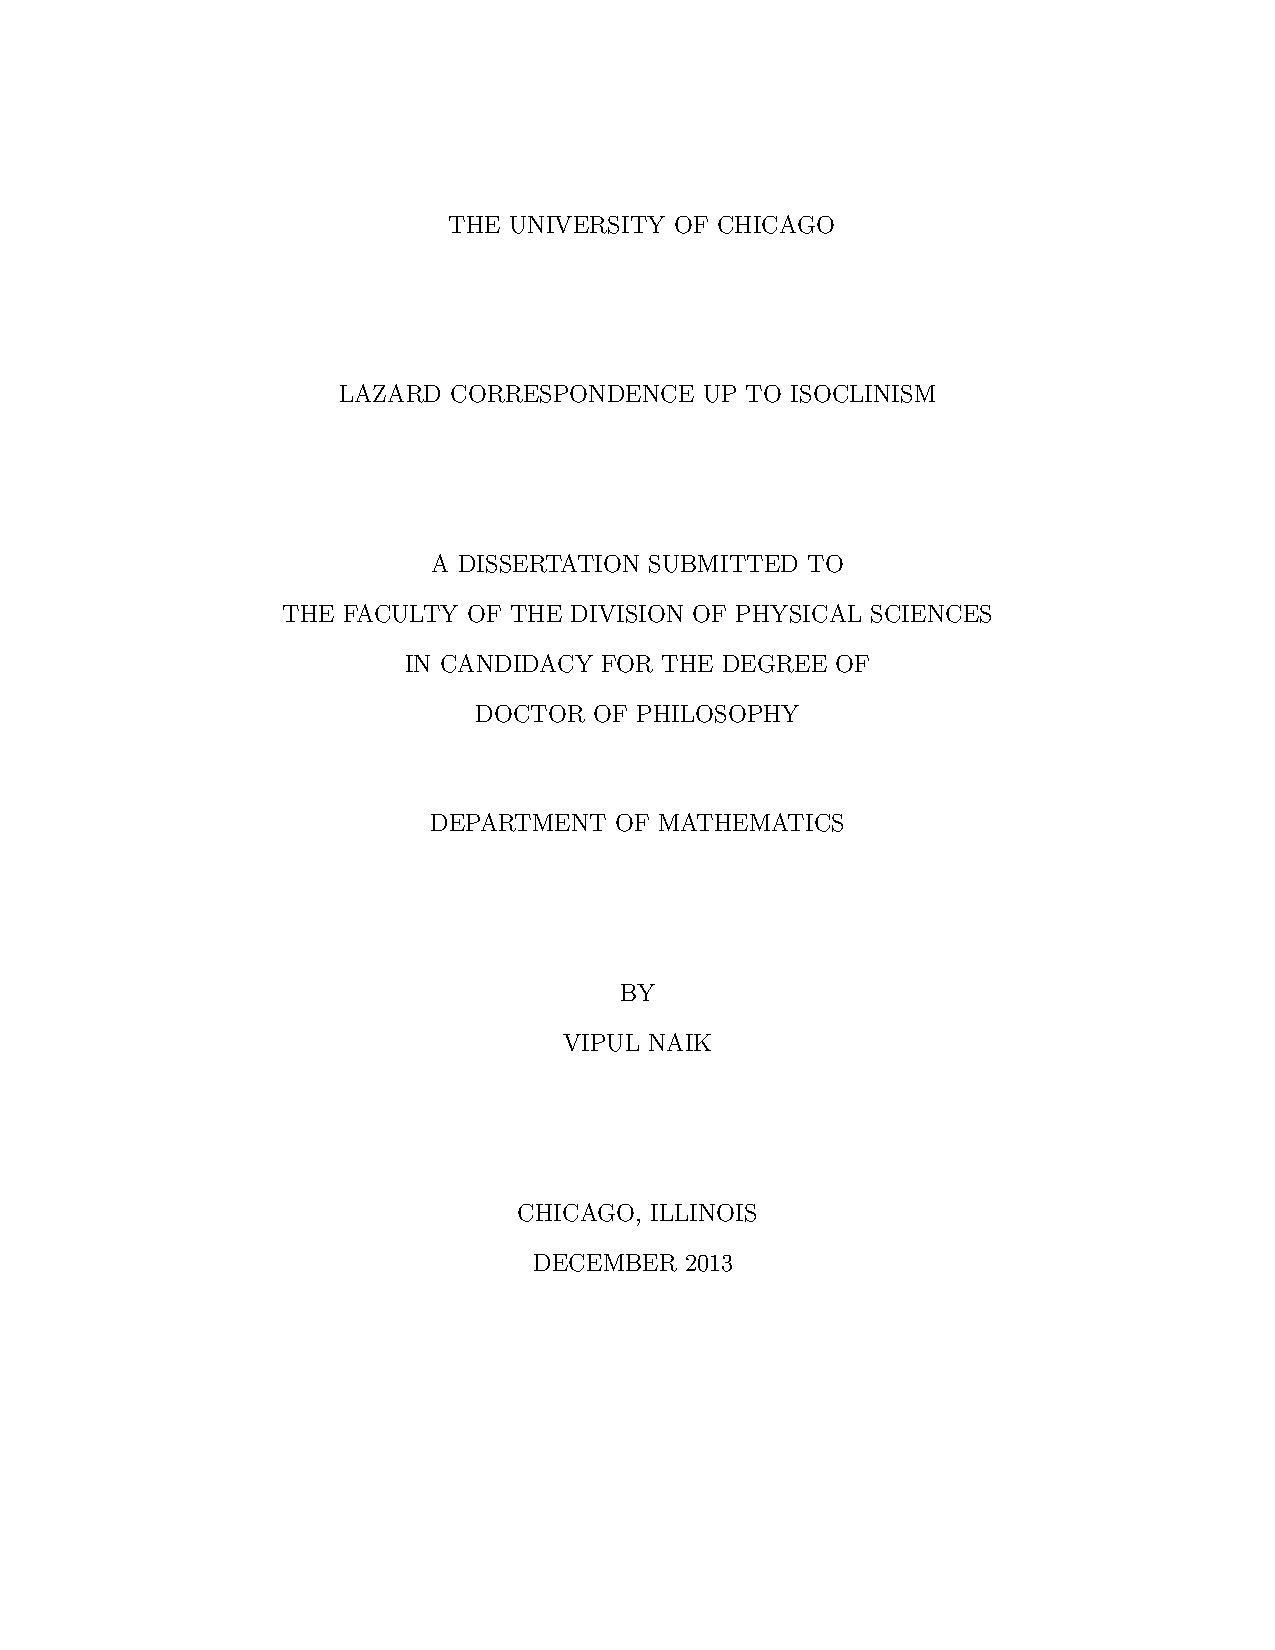
\includepdf[pages={1}]{thesisfrontpage.pdf}

\tableofcontents

\newpage

\section*{Abstract}

In this thesis we generalize the Lazard correspondence, introduced by
Lazard in \cite{Lazardsoriginal}, to a correspondence {\em up to
  isoclinism}. The original Lazard correspondence is a correspondence
between some groups and some Lie rings. The Lazard correspondence up
to isoclinism is a correspondence between some equivalence classes of
groups and some equivalence classes of Lie rings, where the
equivalence relation on both sides is isoclinism. By relaxing the
objects on both sides of the correspondence to equivalence classes up
to isoclinism, we are able to generalize the domain of the
correspondence somewhat. An overview of our proof strategy is in
Section \ref{sec:outline}, and our final results are described in
Section \ref{sec:lcuti}.

A typical application of the original Lazard correspondence is the
situation where, for some prime $p$, the group is a finite $p$-group
of nilpotency class at most $p - 1$ and the Lie ring is a finite
$p$-Lie ring\footnote{This means that the additive group of the Lie
  ring is a finite $p$-group. In other words, the Lie ring is a Lie
  algebra over $\Z/p^k\Z$ for some positive integer $k$.} of
nilpotency class at most $p - 1$.

A typical application of the generalization we describe is the
situation where the group is a finite $p$-group of nilpotency class at
most $p$ and the Lie ring is a finite $p$-Lie ring of nilpotency class
at most $p$. Knowledge of either (the group or the Lie ring)
determines the other only up to isoclinism and not up to
isomorphism. Therefore, this correspondence is suited only for the
study of attributes (of groups or Lie rings) that are invariant under
isoclinism.

In cases where the original Lazard correspondence applies, it refines
the Lazard correspondence up to isoclinism: if a group and Lie ring
are in Lazard correspondence, then they are also in Lazard
correspondence up to isoclinism. The interesting case covered by our
correspondence is the case of finite $p$-groups of nilpotency class
exactly $p$ and finite $p$-Lie rings of nilpotency class exactly
$p$. The original Lazard correspondence no longer applies in this
situation,\footnote{There is a subtle distinction between the global
  and the $3$-local Lazard correspondence that we omit for the
  abstract, but describe in detail later} so our generalization
adds value.

\newpage

\section*{Acknowledgements}

I would like to thank George Glauberman, my research advisor, for help
over many years with the research underlying this thesis and for
detailed feedback on multiple drafts of the thesis. In addition I am
thankful to Peter May, my second adviser, for helping me out with a
number of the proofs and some of the underlying concepts. I would also
like to thank Professor Jonathan Alperin, who provided help in person,
via email, and by lending books and resources. In addition, I am
grateful to Shmuel Weinberger, the Department Chair, and Laurie Wail,
the Graduate Student Administrator, for being very accommodating in
helping me finish my thesis and arranging for financial support.

I am grateful to many mathematicians, both within and outside the
University of Chicago, for answering my many queries related to group
theory and mathematics. A partial list includes Max Horn of Justus
Liebig University Giessen, I. Martin Isaacs of the University of
Wisconsin-Madison, Ronald Solomon of Ohio State University, and Justin
Lynd, an assistant professor at Rutgers University. I am thankful to
Anton Geraschenko and StackExchange for collaborating to create the
mathematics question-and-answer website MathOverflow, and to the
numerous mathematicians who volunteered their time to answering
questions of mine on
MathOverflow\footnote{\url{http://www.mathoverflow.net}}, some of
which have influenced proofs that appear in this thesis. In addition,
I am grateful to the creators of GAP\footnote{Full list of authors at
  \url{http://www.gap-system.org/Contacts/People/authors.html}} for
providing a software that enabled me to play around with and better
understand groups, which are the central actors of my thesis.

I would also like to thank John Wiltshire-Gordon, who, while an
undergraduate at the University of Chicago, worked with me on related
problems. Some of the work we did together was the basis of Section
\ref{sec:bcuti}.

I also greatly enjoyed and benefited from reading the work of the many
mathematicians who are cited in this thesis, including Baer, Lazard,
Hall and Senior, Isaacs, Glauberman, Ellis, Khukhro, and many others
listed in the bibliography.

\newpage

\section*{Background and notation}

\subsection{Background assumed}

This document assumes that the reader is comfortable with group theory
at an advanced undergraduate or beginning graduate student level. At
minimum, the reader's knowledge should be approximately equivalent to
the first six chapters of \cite{DummitFoote}. A knowledge of the
material in \cite{RotmanGT} would make the document easy
reading. There will be particular emphasis on knowledge of the
structure of $p$-groups and nilpotent groups, including knowledge of
the interplay between the upper central series and lower central
series. A review of the most important definitions and basic results
is available in the Appendix, Section \ref{appsec:group-basic}.

Rudimentary familiarity with the ideas of universal algebra and
category theory will be helpful in understanding the motivating
ideas. A review of the most important ideas is available in the
Appendix, Sections \ref{appsec:category} and \ref{appsec:univalg-basic}.

It is assumed that the reader is familiar with the idea of Lie rings,
which can be viewed as Lie algebras over $\mathbb{Z}$, the ring of
integers. However, familiarity with Lie {\em algebras}
over the real numbers or complex numbers will also be sufficient. A
review of some basic definitions from the theory of Lie rings can be
found in the Appendix, Section \ref{appsec:Lie}.

\subsection{Group and subgroup notation}\label{sec:group-notation}

Let $G$ be a group. We will use the following notation throughout this
document.

\begin{itemize}
\item We will use $1$ to denote the trivial subgroup of $G$. Note that
  the same letter $1$ will be used to denote both the trivial group as
  an abstract group and the trivial subgroup in all groups.
\item We will also use $1$ to denote the identity element of $G$.
\item When working with groups that are known to be abelian groups, we
  will use additive notation: $0$ to denote the trivial group and $+$
  to denote the group operation. However, we will use multiplicative
  notation when dealing with abelian subgroups inside a (possibly)
  non-abelian group.
\item $H \le G$ will be understood to mean that $H$ is a sub{\em
  group} of $G$.
\item $Z(G)$ will refer to the center of $G$.
\item $G'$ and $[G,G]$ both refer to the derived subgroup of $G$.
\item $\gamma_c(G)$ refers to the $c^{th}$ member of the lower central
  series of $G$, given as follows: $\gamma_1(G) = G$, $\gamma_2(G) = G'$,
  and $\gamma_{i+1}(G) = [G,\gamma_i(G)]$.
\item $Z^c(G)$ refers to the $c^{th}$ member of the upper central
  series of $G$, given as follows: $Z^0(G)$ is the trivial subgroup,
  $Z^1(G) = Z(G)$, and $Z^{i+1}(G)/Z^i(G) = Z(G/Z^i(G))$ for
  $i \ge 1$.
\item $G^{(i)}$ denotes the $i^{th}$ member of the derived series of
  $G$, given by $G^{(0)} = G$, $G^{(1)} = G'$, and $G^{(i+1)} =
  [G^{(i)},G^{(i)}]$.
\item $\operatorname{Inn}(G)$ is the inner automorphism group of
  $G$. It is canonically isomorphic to the quotient group $G/Z(G)$,
  and we will often abuse notation by treating $\operatorname{Inn}(G)$
  as set-theoretically identical with $G/Z(G)$.
\item $\operatorname{Aut}(G)$ is the automorphism group of $G$. We
  treat $\operatorname{Inn}(G)$ naturally as a subgroup of
  $\operatorname{Aut}(G)$. In fact, $\operatorname{Inn}(G)$ is a
  normal subgroup of $\operatorname{Aut}(G)$.
\item $\operatorname{End}(G)$ is the endomorphism {\em monoid} of $G$,
  i.e., the set of endomorphisms of $G$ with the monoid structure
  given by composition.
\end{itemize}

\subsection{Lie ring and subring notation}\label{sec:lie-ring-notation}

Let $L$ be a Lie ring, i.e., a Lie algebra over $\Z$, the ring of
integers. We will use the following notation throughout this document.

\begin{itemize}
\item We will use $0$ to denote the zero subring of $L$. Note that $0$
  is used to describe both the abstract zero Lie ring and the zero
  subring in every Lie ring.
\item We will also use $0$ to denote the zero element of $L$.
\item $M \le L$ will be understood to mean that $M$ is a Lie subring
  of $L$. This means that it is an additive subgroup of $L$ and is
  closed under the Lie bracket.
\item $Z(L)$ denotes the center of $L$, i.e., the subring of $L$
  comprising those elements whose Lie bracket with any element of $L$
  is zero.
\item $L'$ and $[L,L]$ both refer to the derived subring of $L$.
\item $\gamma_c(L)$ refers to the $c^{th}$ member of the lower central
  series of $L$, given as follows: $\gamma_1(L) = L$, $\gamma_2(L) =
  L'$, and $\gamma_{i+1}(L) = [L,\gamma_i(L)]$.
\item $Z^c(L)$ refers to the $c^{th}$ member of the upper central
  series of $L$, given as follows: $Z^0(L)$ is the trivial subring,
  $Z^1(L) = Z(L)$, and $Z^{i+1}(L)/Z^i(L) = Z(L/Z^i(L))$ for
  $i \ge 1$.
\item $L^{(i)}$ denotes the $i^{th}$ member of the derived series of
  $L$, given by $L^{(0)} = L$, $L^{(1)} = L'$, and $L^{(i+1)} =
  [L^{(i)},L^{(i)}]$.
\item $\operatorname{Inn}(L)$ is the Lie ring of inner derivations of
  $L$. It is canonically isomorphic to the quotient Lie ring $L/Z(L)$,
  and we will often abuse notation by treating $\operatorname{Inn}(L)$
  as set-theoretically identical with $L/Z(L)$.
\item $\operatorname{Der}(L)$ is the Lie ring of all derivations of
  $L$. We treat $\operatorname{Inn}(L)$ naturally as a Lie subring of
  $\operatorname{Der}(L)$. In fact, $\operatorname{Inn}(L)$ is an
  ideal in $\operatorname{Der}(L)$.
\item $\operatorname{Aut}(L)$ is the automorphism group of $L$.
\item $\operatorname{End}(L)$ is the endomorphism {\em monoid} of $L$
  considered as a Lie ring. Note that this is not necessarily closed
  under addition.
\item $\operatorname{End}_{\mathbb{Z}}(L)$ is the endomorphism ring of
  the underlying additive group of $L$. To avoid confusion, we will
  explicitly specify that we are looking at all additive group
  endomorphisms whenever we use this notation.

\end{itemize}

\subsection{Other conventions}

We will adopt these conventions:

\begin{itemize}
\item As a {\em general} rule, when dealing with homomorphisms and
  other similar functions, we will apply functions on the left, in
  keeping with the convention used in most mathematics texts. Thus, $f
  \circ g$ is to be interpreted as saying that the function $g$ is
  applied first and the function $f$ is applied later.
\item For the action of a group on itself, we denote by ${}^gx$ the
  action of $g$ by conjugation on $x$ as a left action, i.e.,
  $gxg^{-1}$. We denote by $x^g$ the action of $g$ by conjugation on
  $x$ as a right action, i.e., $g^{-1}xg$. When stating results whose
  formulation is sensitive to whether we use the left-action
  convention or the right-action convention, we will explicitly state
  the result using both conventions.
\item If using the left-action convention, the group commutator
  $[x,y]$ is defined as $xyx^{-1}y^{-1}$. If using the right-action
  convention, the group commutator $[x,y]$ is defined as
  $x^{-1}y^{-1}xy$.
\end{itemize}

%\chapter{Introduction, outline, and preliminaries}

%\newpage

\section{Introduction}\label{sec:intro}

\subsection{The difference in tractability between groups and abelian groups}

The {\em structure theorem for finitely generated abelian groups},
which in turn leads to a classification of all finite abelian groups,
shows that the structure of {\em abelian} groups is fairly easy to
understand and control. On the other hand, the structure of groups in
general is wild.  Even classifying finite groups is extremely
difficult.

The difficulty is two-fold. On the one hand, the finite simple groups
(which can be thought of as the building blocks of finite groups) have
required a lot of effort to classify. While the original
classification was believed to have been completed around 1980, some
holes in parts of the proof were discovered later and it is believed
that these holes were fixed only around 2004. The only finite simple
abelian groups are the cyclic groups of order $p$. However, there are
$17$ infinite families and $26$ sporadic groups among the finite
simple non-abelian groups. For a quick background on the
classification, see \cite{Asch2004}.

At the other extreme from finite simple groups are the finite
$p$-groups. It is well known that any finite group of order $p^n$ (for
a prime $p$ and natural number $n$) must be a nilpotent group and
therefore it has $n$ composition factors that are all cyclic groups of
order $p$. In other words, there is no mystery about the building
blocks of these groups. Despite this, the multiplicity of ways of
putting the building blocks together makes it very difficult to obtain
a concise description of all the groups of order $p^n$. The general
consensus among people who have studied $p$-groups is that it is
futile to even attempt to obtain a concise description of all the
isomorphism types of groups of order $p^n$, and that it is likely that
no such description exists. Rather, the goal of the study of
$p$-groups is to identify methods that enable us to better understand
the totality of $p$-groups, including aspects that are common to all
of them and aspects that differentiate some $p$-groups from
others. For a description of the state of knowledge regarding
$p$-groups, see \cite{Mann99}.\footnote{Although the article was
  published in 1999, progress has been modest since then.}

This thesis is focused on one small part of the study of finite
$p$-groups.

\subsection{Nilpotent groups and their relation with abelian groups}

A group is termed {\em nilpotent} if it has a central series of finite
length. Nilpotent groups are considerably more diverse in nature than
abelian groups, and as alluded to in the preceding section, even the
finite nilpotent groups are difficult to classify.

A group is termed {\em solvable} if it has a normal series where all
the quotient groups are abelian groups. Solvable groups are
considerably more diverse than nilpotent groups.

Generally, statements that are true for abelian groups fall into one
of these four classes:

\begin{enumerate}
\item The statement does not generalize much further from abelian
  groups
\item The statement generalizes all the way to nilpotent groups but
  not much further
\item The statement generalizes all the way to solvable groups but not
  much further
\item The statement generalizes to all groups, or to a fairly large
  class of groups
\end{enumerate}

It might be worthwhile to attempt to understand why the properties of
being nilpotent and being solvable differ qualitatively, and why the
former is far closer to being abelian than the latter. In an abelian
group, the commutativity relation holds precisely: $ab = ba$ for all
$a$ and $b$ in the group. In general, $ab$ and $ba$ ``differ'' by a
commutator, i.e., $ab = [a,b]ba$ if we use the left action convention
for commutators.

When we consider expressions in a group and try to rearrange the terms
of the expression, the process of rearrangement introduces
commutators. These commutators themselves need to be moved past
existing terms, which introduces commutators between the commutators
and existing terms. In a nilpotent group, we eventually reach a stage
where the iterated commutators that we obtain are central, and
therefore can be freely moved past existing terms. In a solvable
group, such a stage may never arise.

An alternative perspective is that of {\em iterative algorithms}, a
common class of algorithms found in numerical analysis and other parts
of mathematics. An iterative algorithm attempts to find a solution to
a problem by guessing an initial solution and iteratively refining
the guess by identifying and correcting the error in the initial
solution. There are many iterative algorithms that are guaranteed to
terminate only for nilpotent groups, and where the number of steps in
which the algorithm is guaranteed to terminate is bounded by the
nilpotency class of the group. These algorithms work in a single step
for abelian groups, because commutativity allows for the necessary
manipulations to happen immediately. For non-abelian nilpotent groups,
the algorithms work by gradually refining guesses modulo members of a
suitable central series (such as the upper central series or lower
central series).

\subsection{The Lie correspondence: general remarks}\label{sec:lie-correspondence-intro}

The {\em non-abelianness} of groups makes it comparatively difficult
to keep track of group elements and to study the groups. It would be
very helpful to come up with an alternate description of the structure
of a group that replaces the (noncommutative) group multiplication
with a commutative group multiplication, and stores the
noncommutativity in the form of a separate operation. A {\em Lie ring}
(defined in the Appendix, Section \ref{appsec:Lie}) is an example of
such a structure.

For readers familiar with the concept of {\em Lie algebras} over $\R$
or $\mathbb{C}$, note that the definition of Lie ring is similar,
except that the underlying additive group is just an abelian group
(rather than being a $\R$-vector space or $\C$-vector space) and the
Lie bracket is just $\Z$-bilinear rather than being $\R$-bilinear or
$\C$-bilinear. In particular, any Lie algebra over $\R$ or $\C$ is a
Lie ring, but not every Lie ring is a Lie algebra over $\R$ or $\C$,
and even if it is, there may be multiple ways of giving it such a Lie
algebra structure.

The {\em Lie correspondence} is an important correspondence in the
theory of real Lie groups. For an elementary exposition of this
correspondence, see \cite{vsv}. We recall here some of the key
features of the correspondence.

To any finite-dimensional real Lie group, we can functorially
associate a $\R$-Lie algebra called the {\em Lie algebra of the Lie
  group}. The underlying vector space of the Lie algebra is the
tangent space at the identity to the Lie group, or equivalently, the
space of left-invariant vector fields, and the Lie bracket is defined
using the Lie bracket of vector fields. Note that the Lie algebra of a
Lie group depends only on the connected component of the identity.

Additionally, there exists a map, called the {\em exponential map},
from the Lie algebra to the Lie group. This map need not be bijective
globally, but it must be bijective in a small neighborhood of the
identity. The inverse of the map, again defined in a small
neighborhood of the identity, is the {\em logarithm} map. Note that
the exponential map is globally defined, but the logarithm map is
defined only locally.

The association is not quite a correspondence. The problem is that
different Lie groups could give rise to isomorphic Lie
algebras. However, if we restrict attention to {\em connected simply
  connected Lie groups}, then the association becomes a
correspondence, and we can construct a functor in the reverse
direction. Explicitly, the Lie correspondence is the following
correspondence, functorial in both directions:

\begin{center}
  Connected simply connected finite-dimensional real Lie groups
  $\leftrightarrow$ Finite-dimensional real Lie algebras
\end{center}

\subsection{The Lie algebra for the general linear group}\label{sec:lie-correspondence-gln}

Denote by $GL(n,\R)$ the general linear group of degree $n$ over the
field of real numbers, i.e., the group of all invertible $n \times n$
matrices with real entries. Denote by $\mathfrak{g}\mathfrak{l}(n,\R)$ the ``general linear
Lie algebra'' of degree $n$ over $\R$. Explicitly, $\mathfrak{g}\mathfrak{l}(n,\R)$ is the
vector space of all $n \times n$ matrices over $\R$, and the Lie
bracket is defined as $[x,y] := xy - yx$.

$\mathfrak{g}\mathfrak{l}(n,\R)$ is the Lie algebra of $GL(n,\R)$. The
exponential and logarithm maps in this case are the usual matrix
exponential and matrix logarithm maps. The exponential map:

$$\exp: \mathfrak{g}\mathfrak{l}(n,\R) \to GL(n,\R)$$

is defined as:

$$x \mapsto \sum_{i=0}^\infty \frac{x^i}{i!} = 1 + x + \frac{x^2}{2!} + \frac{x^3}{3!} + \dots$$

The matrix exponential is defined for all matrices. However, the
exponential map is neither injective nor surjective:

\begin{itemize}
\item The exponential map is not surjective for any $n$. For $n = 1$,
  this is because the exponential of any real number is a {\em
    positive} real number. A similar observation holds for larger $n$,
  once we observe that the image of the exponential map is inside
  $GL^+(n,\R)$, the subgroup of $GL(n,\R)$ comprising the matrices of
  positive determinant. However, for $n > 1$, the exponential map is
  not surjective even to $GL^+(n,\R)$. For instance, the following
  matrix is not the exponential of any matrix with real entries:

  $$\begin{pmatrix} -1 & 1 \\ 0 & -1 \\\end{pmatrix}$$

\item The exponential map is not injective for $n > 1$. For instance,
  for any positive integer $m$, the following matrix has exponential
  equal to the identity matrix:

  $$\begin{pmatrix} 0 & 1 \\ -4m^2\pi^2 & 0 \\\end{pmatrix}$$
\end{itemize}

Nonetheless, we can find an open neighborhood $U$ of the zero matrix
in $\mathfrak{g}\mathfrak{l}(n,\R)$ and an open neighborhood $V$ of
the identity matrix in $GL(n,\R)$ such that the exponential map is
bijective (and in fact, is a homeomorphism) from $U$ to $V$.

Note that $GL(n,\R)$ is not a connected simply connected Lie group, so
the above is not an instance of the Lie {\em correspondence}.
\subsection{The nilpotent case of the Lie correspondence}

The example of $\mathfrak{g}\mathfrak{l}(n,\R)$ and $GL(n,\R)$
illustrates that the exponential map does not always behave
nicely. However, it turns out that the exponential map behaves much
better when we apply the Lie correspondence in the {\em nilpotent}
case. Explicitly, the nilpotent case of the Lie correspondence is a
correspondence:

\begin{center}
  Connected simply connected finite-dimensional nilpotent real Lie
  groups $\leftrightarrow$ Finite-dimensional nilpotent real Lie
  algebras
\end{center}

In the nilpotent case, it will turn out that the exponential map is
{\em bijective}, and in fact, it defines a homeomorphism from the Lie
algebra to the Lie group. Thus, we can define its inverse, the
logarithm map, {\em globally}.

We now turn to an example.

\subsection{The example of the unitriangular matrix group}\label{sec:unitriangular-lie-correspondence}

A special case of interest for us is the correspondence between the
Lie ring $NT(n,\R)$ of $n \times n$ strictly upper triangular matrices
over $\R$ and the group $UT(n,\R)$ of $n \times n$ upper triangular
matrices over $\R$ with all the diagonal entries equal to $1$. This
correspondence gives a bijection between the underlying sets of
$NT(n,\R)$ and $UT(n,\R)$ via the exponential map. Explicitly, the
matrix exponential defines a bijective set map:

$$\exp: NT(n,\R) \to UT(n,\R)$$

given explicitly as:

$$\exp(x) = e^x = 1 + x + \frac{x^2}{2!} + \dots + \frac{x^{n-1}}{(n - 1)!}$$

Note that this coincides with the usual matrix exponential because
$x^n = 0$ and all higher powers of $x$ are therefore also zero. In
other words, this exponential map is the restriction to $NT(n,\R)$ of
the exponential map described in the preceding section:

$$\exp: \mathfrak{g}\mathfrak{l}(n,\R) \to GL(n,\R)$$

However, {\em unlike} the case of $GL(n,\R)$, the exponential map from
$NT(n,\R)$ to $UT(n,\R)$ is bijective, and in fact, is a
homeomorphism. Topologically, both $NT(n,\R)$ and $UT(n,\R)$ are
homemorphic (i.e., isomorphic in the category of topological spaces) to
the vector space $\R^{\binom{n}{2}}$.

The inverse set map is the matrix logarithm, now defined {\em
  globally}:

$$\log: UT(n,\R) \to NT(n,\R)$$

given explicitly as:

$$\log x := (x - 1) - \frac{(x - 1)^2}{2} + \frac{(x - 1)^3}{3} - \dots + \frac{(-1)^n (x - 1)^{n-1}}{n - 1}$$

\subsection{The Malcev correspondence and Lazard correspondence}\label{sec:intro-malcev-and-lazard}

The {\em Malcev correspondence} is a generalization of the nilpotent
case of the Lie correspondence that applies to algebras over the field
of rational numbers. Explicitly, the correspondence is:

\begin{center}
  Rationally powered nilpotent groups $\leftrightarrow$ Nilpotent $\Q$-Lie algebras
\end{center}

We will define ``rationally powered'' in Section
\ref{sec:group-powering}, but a quick definition for our purpose is
that every element has a unique $n^{th}$ root for every positive
integer $n$. The Malcev correspondence is a purely algebraic
correspondence that does not deal with topological structure. Note
that any $\R$-Lie algebra is a $\Q$-Lie algebra as well. It turns out
that for any nilpotent $\R$-Lie algebra, the Lie correspondence
coincides with the Malcev correspondence. Thus, for instance, under
the Malcev correspondence, the group associated with $NT(n,\R)$ is
$UT(n,\R)$.

The Malcev correspondence has a slight further generalization called
the {\em Lazard correspondence}, introduced by Lazard in
\cite{Lazardsoriginal}. The Lazard correspondence relaxes the
  assumption of being ``rationally powered'' and replaces it with the
  assumption that unique division by specific primes (namely, primes
  that are less than or equal to the nilpotency class) is possible.

If we use the Lazard correspondence in the direction from groups to
Lie rings, then it allows us to convert (a suitable type of) abstract
nilpotent group to a nilpotent Lie ring. The addition operation of the
Lie ring captures the abelian part of the group multiplication,
whereas the Lie bracket captures the non-abelian part of the group
multiplication.

Unfortunately, the Lazard correspondence applies only to {\em some}
nilpotent groups and some nilpotent Lie rings. Specifically, for
finite $p$-groups, it only works for finite $p$-groups where any
subset of size three generates a subgroup of nilpotency class at most
$p - 1$. For the bulk of this document, we will restrict our attention
to the case of small {\em global class}, i.e., the subcorrespondence
that applies to finite $p$-groups of nilpotency class at most $p - 1$.

This means that groups that have higher nilpotency class (a
way of saying that the groups are relatively more non-abelian) cannot
be studied directly using the Lazard correspondence.

We will describe the Malcev correspondence and the Lazard
correspondence in detail in Sections \ref{sec:malcev-correspondence},
\ref{sec:global-lazard-correspondence}, and
\ref{sec:lazard-correspondence}. For a textbook-style presentation of
the correspondence, see Khukhro's book \cite{Khukhro}, Chapters 9 and
10.

\subsection{Our generalization of the Lazard correspondence}

The goal of this document is to describe a generalization of the
Lazard correspondence that works for all $p$-groups of nilpotency
class at most $p$. In other words, it allows us to generalize the
Lazard correspondence to a slightly bigger collection of groups. The
limitation of this generalization is that the correspondence only
works between {\em equivalence classes of groups} and {\em equivalence
  classes of Lie rings}, with each equivalence class containing
multiple isomorphism types. The equivalence relation of interest here
is the equivalence relation of {\em isoclinism}. Informally, two
groups are isoclinic if their commutator maps are equivalent, and two
Lie rings are isoclinic if their Lie bracket maps are equivalent.

\subsection{Similarities and differences between groups and Lie rings}

The theories of groups and Lie rings are {\em structurally
  similar}. For many concepts related to groups, there are analogously
defined concepts for Lie rings. In most cases, the analogous
definition suggests itself naturally. Often, even the proofs are
similar. In some cases, proofs are easier for Lie rings than for
groups, primarily because the Lie bracket is bilinear.

There are {\em some} concepts that make sense only on the group side,
and some concepts that make sense only on the Lie ring
side. Similarly, there are some facts that are true only on the group
side, and some facts that are true only on the Lie ring side.

The closer we are to abelianness, the more structurally similar the
theory for groups is to the theory for Lie rings. In many cases, a
fact is true for nilpotent Lie rings if and only if the ``analogous''
fact is true for nilpotent groups. There are many facts that are true
in {\em general} for Lie rings and are not true in general for groups,
but they are true for nilpotent groups.

In addition to {\em structural similarity}, we will also see some
instances of {\em bijective correspondences} between certain types of
groups and certain types of Lie rings (including the Lie
correspondence and the Lazard correspondence). It will turn out that
{\em analogous concepts} become {\em bijectively correspondent} under
these correspondences. For instance, normal subgroups of groups are
analogous to ideals in Lie rings. The Lazard correspondence between
groups and Lie rings establishes a bijective correspondence between
(certain kinds of) normal subgroups of the group and (certain kinds
of) ideals of the Lie ring.

\subsection{Our central tool: Schur multipliers}

Our goal is to extend the domain of the Lazard correspondence by
relaxing its strictness (from a correspondence up to isomorphism to a
correspondence up to isoclinism). In particular, we are interested in
extending the Lazard correspondence to {\em nilpotency class one
  higher} than where it applies. Thus, the groups
(respectively, Lie rings) of interest to us arise as {\em central
  extensions} where the quotient group (respectively, quotient Lie
ring) is in the domain of the Lazard correspondence.

Rather than directly trying to study the groups and Lie rings, we
study the theory of central extensions for groups and Lie rings. We
first develop the {\em general} theory of such central
extensions. Then, we apply that general theory to the case where the
quotient group (respectively quotient Lie ring) of the central
extension lies in the domain of the Lazard correspondence. In the edge
case of interest where the group is in the domain of the Lazard
correspondence but its central extensions are ``just outside'' the
domain, we can obtain new insights. For instance, if $G$ is a
$p$-group of nilpotency class exactly $p - 1$, it is a Lazard Lie
group. The central extensions with quotient group $G$ are $p$-groups
of nilpotency class either $p - 1$ or $p$. The latter may lie outside
the domain of the Lazard correspondence.

On both the group side and the Lie ring side, the theory of central
extensions is governed by an abelian group called the {\em Schur
  multiplier}. There is a rich theory behind the Schur multiplier, and
it connects with important ideas from algebraic topology and
homological algebra. We will explore the necessary facets of this
theory. Eventually, we will prove (in Theorem
\ref{thm:global-lazard-correspondence-preserves-schur-multipliers})
that if a Lie ring and a group are in Lazard correspondence, then
their Schur multipliers are isomorphic. A version of the statement for
finite $p$-groups appeared as a conjecture in the paper
\cite{SchurmultiplierandLazard} by Eick, Horn, and Zandi in September
2012, stated informally after Theorem 2 of the paper.\footnote{The
  authors write: ``Based on various example computations, see also
  [7], we believe that Theorems 1 and 2 also hold for finite
  $p$-groups of class $p - 1$. However, our proofs do not extend to
  this case.''  The reference [7] alluded to by the authors has not
  yet been published or made available online. For a more detailed
  discussion, see Section
  \ref{sec:global-lazard-correspondence-preserves-schur-multipliers}}
Once the Schur multipliers are established to be isomorphic, it is
easy to establish the Lazard correspondence up to isoclinism.

\subsection{Globally and locally nilpotent}\label{sec:globally-and-locally-nilpotent}

The numbers $2$ and $3$ are particularly significant in the context of
the axiomatization of groups and Lie rings, and they also play an
important role in the Lazard correspondence. $2$ is the maximum of the
arities\footnote{The arity of an operation is the number of inputs it
  takes. For instance, group multiplication has arity $2$. Arity is
  discussed in more detail in the Appendix, Section
  \ref{appsec:univalg-basic}.} of the operations used in the definition
of groups. In particular, this means that if a function between groups
restricts to a homomorphism on every subgroup generated by at most $2$
elements, then the function is globally a homomorphism.

$3$ is the maximum of the number of variables that appear in the
identities that define a group. In particular, this means that if an
algebra has the same signature as a group (i.e., a $0$-ary operation
for the identity, a unary operation for the inverse map, and a binary
operation for the group multiplication), and every subalgebra of the
algebra generated by at most $3$ elements is a {\em group}, then the
algebra is globally a group.

The same is true for Lie rings: the maximum of the arities of the
operations is $2$, and the maximum of the number of terms that appear
in the defining identities is $3$. Thus, any function between Lie
rings that restricts to a homomorphism on subrings generated by sets
of size at most $2$ is globally a homomorphism. Further, given an
algebra with the same signature as a Lie ring, such that every
subalgebra generated by at most $3$ elements becomes a Lie ring with
the induced operations, the algebra as a whole is a Lie ring.

The formulas used in the Lazard correspondence describe the group
operations in terms of the Lie ring operations, and conversely
describe the Lie ring operations in terms of the group operations. The
{\em formulas} themselves refer to a maximum of two elements at a
time. However, the {\em verification} that these formulas work (i.e.,
that starting from a Lie ring, we end up with a group, or that
starting from a group, we end up with a Lie ring) relies on looking at
three elements at a time. For instance, to verify that a formula
describing group operations in terms of Lie ring operations does
indeed define a group structure, we need to verify the associativity
identity for three arbitrary elements. Similarly, to verify that a
formula describing Lie ring operations in terms of group operations
does indeed define a Lie ring structure, we need to verify the
associativity of addition, bilinearity, and Jacobi identity for the
Lie ring operations. Each of these identities requires considering
three arbitrary elements at a time.

Thus, the conditions that we work out on groups (respectively, Lie
rings) pertaining to the Lazard correspondence are $3$-local
conditions: they are conditions on what subgroups (respectively, Lie
subrings) generated by subsets of size at most three look like.

\subsection{The structure of this document}

The document is quite long despite the fact that the eventual proofs
are relatively short and simple. The reason is that the existing
literature we draw upon is fragmented. We draw on literature with
these five broad themes:

\begin{itemize}
\item Isoclinism and homoclinism.
\item Schur multiplier and the relation with group extension theory.
\item Exterior square and its generalizations.
\item The Lazard correspondence.
\item The behavior of groups and Lie rings where we can divide by
  specific primes.
\end{itemize}

Each of these themes has a well-developed body of literature. However,
the connections between these ideas are not emphasized in the
literature, and it often requires a careful reading to glean
them. Thus, it would not be sufficient to simply cite the relevant
literature. We use the next few sections to develop all the necessary
background material in preparation for our results.

Our presentation will follow these features:

\begin{itemize}
\item For the foundational sections, we will systematically alternate
  sections between groups and Lie rings. A section about groups will
  develop a concept or construct in the context of groups. The next
  section about Lie rings will develop the analogous concept or
  construct in the context of Lie rings. To the extent possible, we
  will follow parallel modes of presentation in the two
  sections. Differences between the sections will be noted at the
  beginnings of the relevant sections.
\item For the foundational sections, we will often begin by discussing
  a concept in the context of groups or Lie rings in the abstract, and
  then discuss an analogous concept in the context of extensions of
  groups or Lie rings. This will be done somewhat in reverse in the
  later sections, where we sometimes prove a result in the context of
  extensions (of groups or Lie rings) and {\em then} apply that to
  prove the result in the context of groups or Lie rings. This will be
  our {\em modus operandi} for the crucial proofs.
\item Our key results involve generalizing certain correspondences
  (the Baer correspondence and Lazard correspondence) to a larger
  domain, but with a coarser equivalence relation (of isoclinism). For
  each correspondence that we generalize, we first explicitly
  describe the known correspondence and its key attributes (in one
  or more sections), and then describe our generalization.
\end{itemize}

\subsection{For a quick reading}

For readers who wish to understand the main results without delving
into background concepts in unnecessary depth, the following reading
sequence will work:

\begin{enumerate}
\item Chapter 1 (Introduction, outline, and preliminaries):
  \begin{itemize}
  \item Section \ref{sec:outline} contains the outline of our main
    proof techniques. It is worth reading in its entirety.
  \item Section \ref{sec:abelian-lie-correspondence} (The abelian Lie
    correspondence): The contents of this section are straightforward,
    but it is worth reading because the methods used in this section
    form a template for later, more complicated, correspondences.
    \end{itemize}
\item Chapter 2 (Isoclinism and homoclinism: basic theory):
  \begin{itemize}
  \item Section \ref{sec:isoclinism-and-homoclinism} (Isoclinism and
    homoclinism of groups): It suffices to read Sections
    \ref{sec:isoclinism-definition} -- \ref{sec:homoclinism-category}, and
    the statements of the theorems in Section
    \ref{sec:homoclinism-misc-results}. Readers already familiar with
    the definitions can skip this section and return if needed.
  \item Section \ref{sec:isoclinism-and-homoclinism-lie} (Isoclinism
    and homoclinism of Lie rings): It suffices to read Section
    \ref{sec:isoclinism-definition-lie}. Readers already familiar with
    the definitions can skip this section and return if
    needed. Readers who thoroughly understand the general analogy
    between groups and Lie rings can extrapolate the definitions and
    results of this section from the preceding one, and hence may skip
    this section.
  \end{itemize}
\item Chapter 3 (Extension theory):
  \begin{itemize}
  \item Section \ref{sec:ses-group} (Short exact sequences of groups):
    Readers already familiar with the basics of short exact sequences
    and central extensions can read Sections
    \ref{sec:second-cohomology-group-classify-extensions} and
    \ref{sec:homomorphism-central-extensions}.
  \item Section \ref{sec:ses-lie} (Short exact sequences and central
    extensions of Lie rings): Readers who understood the preceding
    section (Section \ref{sec:ses-group}), and understand how the
    analogy between groups and Lie rings works, can skip this section.
  \item Section \ref{sec:cohomology-explicit} (Explicit description of
    second cohomology group): This section can be skipped without loss
    of continuity. The material in this section helps with understanding
    Section \ref{sec:baer-correspondence-cocycle-level}. However, the
    latter can also be skipped without loss of continuity.
  \item Section \ref{sec:exteriorsquare-and-homoclinism} (Exterior
    square, Schur multiplier, and homoclinism): This section is
    important to understand because it lays the foundation for later
    material, and the presentation is non-standard. Readers may skip
    proofs, many of which are tedious, and focus on the statements of
    the results.
  \item Section \ref{sec:exteriorsquare-and-homoclinism-lie} (Exterior
    square, Schur multiplier, and homoclinism for Lie rings): Apart from
    Section \ref{sec:free-lie-ring-on-abelian-group}, this section is
    mostly analogous to the preceding section. Hence, the rest of the
    section can be skipped.
  \item Section \ref{sec:schur-multiplier-and-second-cohomology}: This
    section is important to understand because it lays the foundation
    for later material, and the presentation is non-standard. Readers
    may skip proofs, many of which are tedious, and focus on the
    statements of the results.
  \item Section \ref{sec:schur-multiplier-and-second-cohomology-lie}:
    This section may be skipped by readers who have a thorough
    understanding of the preceding section and understand how the
    analogy between groups and Lie rings works.
  \item Sections \ref{sec:exterior-and-tensor-product} and
    \ref{sec:exterior-and-tensor-product-lie} (Exterior and tensor
    products for groups and Lie rings respectively): These sections can
    be skipped without loss of continuity, and interested readers can
    refer back to the explicit descriptions as needed later.
  \item Sections \ref{sec:free-nilpotent-groups-homology} and
    \ref{sec:free-nilpotent-lie-homology}: These are worth skimming for
    their main results.
  \end{itemize}
\item Chapter 4 (Powering over sets of primes):
  \begin{itemize}
  \item Section \ref{sec:group-powering} (Groups powered over sets of
    primes): Readers would benefit by reading the part of Section
    \ref{sec:group-powering} up to and including Section
    \ref{sec:divisible-and-torsion-free} in order to familiarize
    themselves with the definitions. Some of the results presented in
    the rest of the section are useful, but they can be revisited as
    necessary.
  \item Section \ref{sec:lie-ring-powering} (Lie rings powered over sets
    of primes): It suffices to read Section
    \ref{sec:lie-ring-powering-def}.
  \item Section \ref{sec:free-powered-groups-and-powering-functors}
    (Free powered groups and powering functors): The results in Sections
    \ref{sec:root-set} and \ref{sec:pi-powered-isoclinism-results} are
    the most important. The rest of the section may be skimmed.
  \item Section \ref{sec:free-powered-lie-rings-and-powering-functors}
    (Free powered Lie rings and powering functors): The results here are
    analogous to the preceding section, though the proofs are more
    straightforward. The section can be skipped and returned to as
    needed.
  \end{itemize}
\item Chapter 5 (Baer correspondence):
  \begin{itemize}
  \item Sections \ref{sec:baer-correspondence-basics} and
    \ref{sec:baer-correspondence-more} (Baer correspondence): It suffices
    to read Sections
    \ref{sec:baer-lie-definitions}-\ref{sec:baer-lie-ring-to-group} and
    Section \ref{sec:baer-p-group-case}. However, readers may benefit
    from skimming both sections in their entirety in order to get a
    better sense.
  \item Section \ref{sec:baer-correspondence-definition-relaxation} may
    be skipped without loss of continuity.
  \item Section \ref{sec:bcuti} (Baer correspondence up to isoclinism):
    Reading the whole section is strongly recommended, but readers may
    skip Section \ref{sec:baer-correspondence-cocycle-level} without
    loss of continuity.
  \item Section \ref{sec:bcuti-ex} contains interesting examples worth
  reading but may be skipped without loss of continuity.
  \end{itemize}
\item Chapter 6 (The Malcev and Lazard correspondences):
  \begin{itemize}
  \item Sections \ref{sec:adjoint-exp-log} and
    \ref{sec:free-nilpotent-exp-log} (adjoint groups, exponential and
    logarithm maps, and free nilpotent groups): These sections may be
    skimmed without reading the proofs. They provide technical
    background for Section \ref{sec:bch}.
  \item Section \ref{sec:bch} (Baker-Campbell-Hausdorff formula): This
    section should be read in its entirety. Readers may benefit from
    concentrating on the statements of the theorems and skimming the
    proofs.
  \item Section \ref{sec:inverse-bch}: This section is partly analogous
    to Section \ref{sec:bch}, so aside from the introduction, it may be
    skimmed.
  \item Sections \ref{sec:malcev-correspondence},
    \ref{sec:global-lazard-correspondence}, and
  \ref{sec:lazard-correspondence} (Malcev correspondence, global
  Lazard correspondence, and Lazard correspondence): These sections
  are worth reading, though people familiar with the correspondences
  may skim them.
  \end{itemize}
\item Chapter 7 (Generalizing the Lazard correspondence to a
  correspondence up to isoclinism):
  \begin{itemize}
  \item Section
    \ref{sec:group-commutator-and-lie-bracket-ito-each-other} (Group
    commutator and Lie bracket in terms of each other) is important.
  \item Section
    \ref{sec:lazard-correspondence-commutativity-relation-central-series}
    may be skimmed.
  \item The theorems in Section \ref{sec:malcev-lazard-free} are
    important as stepping stones for the main results. However, the
    proofs are unilluminative and may be skipped.
  \item The results in Sections
    \ref{sec:homology-of-powered-nilpotent-groups} and
    \ref{sec:homology-of-powered-nilpotent-lie-rings} are important, but
    the proofs may again be skipped.
  \item Sections \ref{sec:commutator-and-lie-bracket-like-maps} and
    \ref{sec:lcuti} are extremely important and should be read
    carefully, though the proofs may be skimmed.
  \end{itemize}
\item Chapter 8 (Applications and possible extensions): Sections
  \ref{sec:applications} and \ref{sec:possible-extensions} may be of
  interest to readers who want to understand potential applications.
\item Readers may refer to the sections in the Appendix based on their
  level of interest. Sections \ref{appsec:background-grouptheory},
  \ref{appsec:abstract-nonsense}, and \ref{appsec:nilpotent} cover
  technical background at the advanced undergraduate or beginning
  graduate level that is useful for understanding the main results of
  the thesis. Section \ref{appsec:homologism-theory} covers a general
  theory that is helpful for understanding potential generalizations
  of the results presented here.
\end{enumerate}

%\newpage

\section{Outline of our main results}\label{sec:outline}

This section provides an overview of our main results and the strategy
we will use to prove these results. Some of the technical details in
this section may be accessible only to people with a strong background
in group theory and some prior familiarity with the Lazard
correspondence. However, all readers should be able to understand the
ideas at a broad level.

\subsection{The Lazard correspondence: a rapid review}

The Lazard correspondence is a correspondence between certain kinds of
groups and certain kinds of Lie rings. The groups, called {\em Lazard
  Lie groups}, satisfy a condition relating the set of primes over
which they are powered and the nilpotency class of subgroups generated
by subsets of size at most three. The Lie rings, called {\em Lazard
  Lie rings}, satisfy a similar condition relating the set of primes
over which they are powered and the nilpotency class of Lie subrings
generated by subsets of size at most three. The precise definition of
the Lazard correspondence is in Section
\ref{sec:lazard-correspondence}. A somewhat easier case of the
correspondence, called the {\em global} Lazard correspondence, is
described in Section \ref{sec:global-lazard-correspondence}. The
global Lazard correspondence imposes a restriction on the nilpotency
class of the whole group and of the whole Lie ring. It is more narrow
than the Lazard correspondence but easier to deal with.

For a Lie ring $L$, the corresponding group, $\exp(L)$, has the {\em
  same underlying set} as $L$, and the group operations are defined in
terms of the Lie ring operations based on fixed formulas. Explicitly,
the group multiplication is defined in terms of the Lie ring
operations using the {\em Baker-Campbell-Hausdorff formula}. The
Baker-Campbell-Hausdorff formula is described in detail in Section
\ref{sec:bch}. Technically, the formula is different for different
values of the ($3$-local) nilpotency class, but we can use a single
infinite series whose truncations give all the formulas.

For a group $G$, the corresponding Lie ring, denoted $\log(G)$, has
the {\em same underlying set} as $G$, and the Lie ring operations are
defined in terms of the group operations based on fixed formulas
called the {\em inverse Baker-Campbell-Hausdorff formulas} (one
formula describing the Lie ring addition and another formula
describing the Lie bracket in terms of the group operations). The
inverse Baker-Campbell-Hausdorff formulas are described in Section
\ref{sec:inverse-bch}.

$\exp$ and $\log$ define functors between appropriately defined
subcategories of the category of groups and the category of Lie rings,
and the functors are two-sided inverses of each other. Thus, they
establish an isomorphism of categories over the category of
sets\footnote{This means an isomorphism of categories that preserves
  the underlying set} between the relevant subcategories of the
category of groups and the category of Lie rings.

\subsection{Isoclinism: a rapid review}

An {\em isoclinism of groups} is a pair of group isomorphisms, one
between their inner automorphism groups and the other between their
derived subgroups, that are compatible with the commutator
map. Intuitively, we can think of an isoclinism of groups as an
equivalence between the commutator structures of the two groups. We
will define and discuss isoclinisms in Section
\ref{sec:isoclinism-and-homoclinism}. 

There is a similar notion of {\em isoclinism of Lie rings} (that uses
the inner derivation Lie ring, the derived subring, and the Lie
bracket) that we will define and discuss in Section
\ref{sec:isoclinism-and-homoclinism-lie}. Intuitively, we can think of
an isoclinism of Lie rings as an equivalence between the Lie bracket
structures of the Lie rings.

We can use isoclinism of groups to define an {\em equivalence
  relation} on the collection of groups. Analogously, we can use
isoclinism of Lie rings to define an equivalence relation on the
collection of Lie rings.

\subsection{The Lazard correspondence up to isoclinism}

The Lazard correspondence up to isoclinism combines the idea of the
Lazard correspondence and the idea of isoclinism. For a Lie ring $L$
and a group $G$, a Lazard correspondence up to isoclinism includes two
pieces of data satisfying a compatibility condition:

\begin{itemize}
\item A Lazard correspondence up to isomorphism between
  $\operatorname{Inn}(L)$ and $\operatorname{Inn}(G)$. This can be
  viewed as an isomorphism of groups between
  $\exp(\operatorname{Inn}(L))$ and $\operatorname{Inn}(G)$ or as an
  isomorphism of Lie rings between $\operatorname{Inn}(L)$ and
  $\log(\operatorname{Inn}(G))$.
\item A Lazard correspondence up to isomorphism between $L'$ and
  $G'$. This can be viewed as an isomorphism of groups between
  $\exp(L')$ and $G'$ or as an isomorphism of Lie rings between $L'$
  and $\log(G')$.
\end{itemize}

The compatibility condition is tricky to specify. Naively, we might
expect that the compatibility condition would say that the isomorphism
converts the Lie bracket map $\operatorname{Inn}(L) \times
\operatorname{Inn}(L) \to L'$ to the commutator map
$\operatorname{Inn}(G) \times \operatorname{Inn}(G) \to G'$. The
problem with this naive specification is that even with the ordinary
Lazard correspondence, the Lie bracket of the Lie ring does not
coincide with the commutator of the group. They {\em do} coincide when
the class is at most two, and we discuss this special case, the {\em
  Baer correspondence up to isoclinism}, in Section \ref{sec:bcuti}.

%% For the Lazard correspondence in higher class, the Lie bracket and
%% commutator map are intimately related, but not equal. The relationship
%% between them has a flavor similar to composition with a unipotent
%% transformation. Explicitly, if the commutator of two elements in the
%% group is trivial, there Lie bracket in the Lie ring is zero, and vice
%% versa.

To handle higher class, we need to first derive a formula valid for
the usual Lazard correspondence that expresses the Lie bracket in
terms of the commutator, and in the reverse direction, we need to
derive a formula valid for the usual Lazard correspondence that
expresses the commutator in terms of the Lie bracket. The
compatibility condition we impose will make use of these formulas. The
formulas themselves are described in Section
\ref{sec:group-commutator-and-lie-bracket-ito-each-other}. The
compatibility condition based on these formulas is described in detail
in Section \ref{sec:lcuti}.


\subsection{The existence question}\label{sec:existence-question}

Defining the Lazard correspondence up to isoclinism is relatively
easy. The harder part is establishing sufficient conditions for the
existence of objects on the other side, i.e., establishing sufficient
conditions for the existence of groups that are in Lazard
correspondence up to isoclinism with a given Lie ring, and
establishing sufficient conditions for the existence of Lie rings that
are in Lazard correspondence up to isoclinism with a given group.

The results that we would like to aim for are:

\begin{itemize}

\item For a Lie ring $L$, if both $\operatorname{Inn}(L)$ and $L'$ are
  Lazard Lie rings, then we can find a group $G$ such that $L$ is in
  Lazard correspondence up to isoclinism with $G$.
\item For a group $G$, if both $\operatorname{Inn}(G)$ and $G'$ are
  Lazard Lie groups, then we can find a Lie ring $L$ such that $L$ is
  in Lazard correspondence up to isoclinism with $G$.
\end{itemize}

Unfortunately, the proofs of these statements at a general level
require more machinery than we can manage in this thesis. We
therefore restrict our proofs here to the case of the global Lazard
correspondence. The precise statements of the results we will prove
are in Section \ref{sec:lcuti}. Essentially, we restrict attention to
groups that satisfy global assumptions on the set of primes over which
they powered, and for which the inner automorphism group and derived
subgroup are both in the domain of the global Lazard correspondence.

The strategy that we use to demonstrate these facts is somewhat
roundabout. Instead of trying to answer the question directly, we try
to answer the question in the more general context of central
extensions of groups and Lie rings. We will then apply the results
that we obtain to the central extensions with short exact sequences:

$$0 \to Z(G) \to G \to G/Z(G) \to 1$$

and

$$0 \to Z(L) \to L \to L/Z(L) \to 0$$

We outline below the argument in the direction from Lie rings to groups.

We begin by viewing $L$ as an extension with central subring $Z(L)$
and quotient ring $L/Z(L) \cong \operatorname{Inn}(L)$. We obtain the
corresponding Lie bracket map $\operatorname{Inn}(L) \times
\operatorname{Inn}(L) \to L'$. We then obtain a desired commutator map
$\exp(\operatorname{Inn}(L)) \times \exp(\operatorname{Inn}(L)) \to
\exp(L')$ by using the formula describing the commutator map in terms
of the Lie bracket map. Finally, we demonstrate the existence of a
group $G$ that realizes this commutator map.

\subsection{The realization of isoclinism types}

We will show that equivalence classes of groups up to isoclinism can
be described by storing the commutator structure in an abstract
fashion, without reference to an actual group in that equivalence
class.

This will be useful to the final step of our proof of existence
established above: instead of directly trying to construct the groups
in the equivalence class up to isoclinism, we construct the commutator
structure. In the notation above, we construct the desired commutator
map $\exp(\operatorname{Inn}(L)) \times \exp(\operatorname{Inn}(L))
\to \exp(L')$.

Below, we provide a few more details about how we store the commutator
structure abstractly. This discussion may be accessible only to people
familiar either with group cohomology or with some other type of
cohomology theory that is structurally similar. Note also that the
group $G$ that we use here is not the same as the group $G$ used in
Section \ref{sec:existence-question}. In fact, to apply what we
discuss below to Section \ref{sec:existence-question}, we would need
to set the group $A$ below to $\exp(Z(L))$ and set the group $G$ below
to $\exp(L/Z(L))$.

{\em Technical details}: In Sections
\ref{sec:exteriorsquare-and-homoclinism} and
\ref{sec:schur-multiplier-and-second-cohomology}, we will show that we
can classify central extensions up to isoclinism using a homomorphism
from the Schur multiplier. Explicitly, when considering central
extensions with central subgroup $A$ and quotient group $G$, we can
determine the type of the extension up to isoclinism by considering
the induced map $M(G) \to A$ where $M(G)$ is the Schur multiplier of
$G$. We will relate this to the universal coefficient theorem short
exact sequence described in Section \ref{sec:ses-uct}.

\begin{equation*}
  0 \to \operatorname{Ext}^1_{\mathbb{Z}}(G^{\operatorname{ab}},A) \to H^2(G;A) \to \operatorname{Hom}(M(G),A) \to 0
\end{equation*}

The key aspect of the above short exact sequence that is relevant for
the existence question is the {\em surjectivity} of the map:

$$H^2(G;A) \to \operatorname{Hom}(M(G),A)$$

Thus, the homomorphism from $M(G)$ to $A$ describes the equivalence
class of extensions up to isoclinism, and every homomorphism from
$M(G)$ to $A$ describes some eqiuvalence class of extensions.

For results in the opposite direction, we develop a similar theory for
Lie rings.
\subsection{Powering assumptions}

One complication that arises in the discussion of the Lazard
correspondence and its generalizations is that the formulas involved
require taking $p^{th}$ roots for some primes $p$. Thus, in order to
make sense of these expressions, we need to develop a basic theory of
groups and Lie rings where these operations make sense. We develop
that basic theory in Sections \ref{sec:group-powering} and
\ref{sec:free-powered-groups-and-powering-functors} (for groups) and
in Sections \ref{sec:lie-ring-powering} and
\ref{sec:free-powered-lie-rings-and-powering-functors} (for Lie
rings).

\subsection{Global Lazard correspondence preserves Schur multipliers}

To complete the proof, we need to demonstrate that the global Lazard
correspondence behaves well with respect to the structures that we use
to classify extensions up to isoclinism. Explicitly, we need to show
that if $L = \log(G)$ and $G = \exp(L)$, then the Schur multipliers
$M(L)$ and $M(G)$ are canonically isomorphic, and also that the
exterior squares $L \wedge L$ and $G \wedge G$ are in Lazard
correspondence.  We will demonstrate these facts in Sections
\ref{sec:homology-of-powered-nilpotent-groups} and \ref{sec:lcuti}
(specifically, in Theorem
\ref{thm:global-lazard-correspondence-preserves-schur-multipliers}). A
version of the statement for finite $p$-groups appeared as a
conjecture in the paper \cite{SchurmultiplierandLazard} by Eick, Horn,
and Zandi in September 2012, stated informally after Theorem 2 of the
paper. Some technical details of our proof idea follow.

{\em Technical details}: The key idea behind our proof is to express
our group as a quotient group of a free powered nilpotent group of
class one more. Using a nilpotency class of one more allows us to use
a variant of the Hopf formula to calculate the Schur multiplier, as
described in \ref{sec:hopf-formula-class-one-more} and
\ref{sec:hopf-formula-pi-powered-class-one-more}. We can perform a
similar construction on the Lie ring side. We now show that the groups
used to compute the Schur multiplier of the group are in Lazard
correspondence with the Lie rings used to compute the Schur multiplier
of the Lie ring. The reason this is nontrivial is that the free
nilpotent group and free nilpotent Lie ring of class one more need not
themselves be in Lazard correspondence. We need to show that despite
this, the groups that we eventually use in the formula for computing
the Schur multiplier are in Lazard correspondence.


%\newpage

\section{The abelian Lie correspondence}\label{sec:abelian-lie-correspondence}

This section describes an obvious and straightforward correspondence:
the correspondence between abelian groups and abelian Lie rings. An
abelian Lie ring is a Lie ring that has trivial Lie bracket. Basic
definitions related to Lie rings can be found in the Appendix, Section
\ref{appsec:Lie}.

All assertions made here are trivial to prove. The purpose of this
section is to set up a basic prototype for the Lazard correspondence.

\subsection{Abelian groups correspond to abelian Lie rings}\label{sec:abelian-lie-correspondence-def}

We establish the abelian Lie correspondence:

\begin{center}
  Abelian groups $\leftrightarrow$ Abelian Lie rings
\end{center}

The correspondence works as follows.

\begin{itemize}
\item From groups to Lie rings: Given an abelian group $G$, the
  corresponding abelian Lie ring $\log G$ is defined as the Lie ring whose
  underlying additive group coincides with $G$, and where the Lie
  bracket is trivial.
\item From Lie rings to groups: Given an abelian Lie ring $L$, the
  corresponding abelian group $\exp L$ is defined as the underlying
  additive group of $L$.
\end{itemize}

Note that the symbols $\exp$ and $\log$ here are being used as
abstract symbols. They do not describe exponential and logarithm
maps in the conventional sense of the term. The relationship with the
usual notions of exponential and logarithm will become clearer in
subsequent sections leading up to the definition of the Lazard
correspondence.

\subsection{Preservation of homomorphisms: viewing $\exp$ and $\log$ as functors}\label{sec:abelian-lie-correspondence-homomorphism-preservation}

The following observations follow immediately from the definitions:

\begin{itemize}
\item $\log$ defines a functor from abelian groups to abelian Lie
  rings: Suppose $G_1$ and $G_2$ are abelian groups and $\varphi:G_1
  \to G_2$ is a group homomorphism. Then, there exists a unique Lie
  ring homomorphism $\log(\varphi): \log(G_1) \to \log(G_2)$ that has
  the same underlying set map as $\varphi$.
\item $\exp$ defines a functor from abelian Lie rings to abelian
  groups: Suppose $L_1$ and $L_2$ are abelian Lie rings and $\varphi:L_1
  \to L_2$ is a Lie ring homomorphism. Then, there exists a unique
  group homomorphism $\exp(\varphi): \exp(L_1) \to \exp(L_2)$ that has
  the same underlying set map as $\varphi$.
\item The $\log$ and $\exp$ functors are two-sided inverses of each
  other: This assertion has four parts:
  \begin{itemize}
    \item For every abelian group $G$, $G = \exp(\log(G))$. 
    \item For every abelian Lie ring $L$, $L = \log(\exp(L))$.
    \item For every group homomorphism $\varphi:G_1 \to G_2$ of
      abelian groups, $\exp(\log(\varphi)) = \varphi$.
    \item For every Lie ring homomorphism $\varphi:L_1 \to L_2$ of
      abelian Lie rings, $\log(\exp(\varphi)) = \varphi$.
  \end{itemize}
\end{itemize}

The upshot of these is that the category of abelian groups and the
category of abelian Lie rings are isomorphic categories, with the
$\log$ and $\exp$ functors providing the isomorphisms.
\subsection{Isomorphism over Set}

Consider the following two categories:

\begin{itemize}
\item The category of abelian groups, with the forgetful functor to
  the category of sets that sends each abelian group to its underlying
  set.
\item The category of abelian Lie rings, with the forgetful functor to
  the category of sets that sends each abelian Lie ring to its
  underlying set.
\end{itemize}

The correspondence we established above (in Sections
\ref{sec:abelian-lie-correspondence-def} and
\ref{sec:abelian-lie-correspondence-homomorphism-preservation})
establishes an {\em isomorphism of categories over Set} between the
two categories. There are two parts to this statement:

\begin{itemize}
\item The correspondence establishes an isomorphism between the
  category of abelian groups and the category of abelian Lie rings:
  The functor in the direction from groups to Lie rings is the $\log$
  functor. The functor in the direction from Lie rings to groups is
  the $\exp$ functor. The details are in the preceding section
  (Section
  \ref{sec:abelian-lie-correspondence-homomorphism-preservation}).
\item This isomorphism has the property that applying it and then
  applying the forgetful functor to the category of sets gives the
  same result as directly applying the forgetful functor to the
  category of sets. This is a category-theoretic way of saying that
  the abelian group and abelian Lie ring have the same underlying set,
  and that the set maps that are group homomorphisms are precisely the
  same as the set maps that are Lie ring homomorphisms.
\end{itemize}

\subsection{Equality of endomorphism monoids and of automorphism groups}\label{sec:abelian-lie-correspondence-aut-end}

Suppose $L$ is an abelian Lie ring and $G = \exp(L)$, so that $L =
\log(G)$. The functors $\exp$ and $\log$ are isomorphisms of
categories, hence they induce isomorphisms between the endomorphism
monoids. Further, since these isomorphisms of categories preserve the
underlying set, the isomorphism between the endomorphism monoids sends
each Lie ring endomorphism to a corresponding group endomorphism that
is {\em the same as a set map}. Explicitly, the map
$\exp:\operatorname{End}(L) \to \operatorname{End}(G)$ is an
isomorphism. Further, for $\varphi \in \operatorname{End}(L)$, the
corresponding map $\exp(\varphi) \in \operatorname{End}(G)$ coincides
with $\varphi$ as a set map. The isomorphism induced by $\exp$ between
the endomorphism monoids $\operatorname{End}(L)$ and
$\operatorname{End}(G)$ restricts to an isomorphism between the
automorphism groups $\operatorname{Aut}(L)$ and
$\operatorname{Aut}(G)$.

\subsection{The correspondence up to isomorphism}\label{sec:abelian-lie-correspondence-up-to-isomorphism}

We have so far considered the correspondence at the level of
individual groups and Lie rings:

\begin{center}
  Abelian groups $\leftrightarrow$ Abelian Lie rings
\end{center}

The correspondence defines an isomorphism of categories, and thus it
descends to a correspondence between equivalence classes up to
isomorphism on both sides, giving a correspondence:

\begin{center}
  Isomorphism classes of abelian groups $\leftrightarrow$ Isomorphism classes of abelian Lie rings
\end{center}

Suppose $L$ is an abelian Lie ring and $G$ is an abelian
group. Specifying an abelian Lie correspondence {\em up to
  isomorphism} between $L$ and $G$ amounts to specifying one of the
following two equivalent pieces of data:

\begin{itemize}
\item An isomorphism of groups from $\exp L$ to $G$.
\item An isomorphism of Lie rings from $\log G$ to $L$.
\end{itemize}

A common convention used to provide this data is to provide one of these:

\begin{itemize}
\item A {\em set} map $\exp:L \to G$ that, viewed as a set map from
  $\exp(L)$ to $G$, becomes a group isomorphism.
\item A {\em set} map $\log:G \to L$ that, viewed as a set map from
  $\log(G)$ to $L$, becomes a Lie ring isomorphism.
\end{itemize}

In other words, we can specify the data in the form of one of these set maps:

$$\exp: L \to G, \log: G \to L$$

The set maps $\log$ and $\exp$ are two-sided inverses of each other.

It will turn out, later, that actual exponential and logarithm maps,
with the usual power series expansions, occurring inside an
associative ring, provide examples of an abelian Lie correspondence up
to isomorphism.

In cases where we want to emphasize that we are talking of the abelian
Lie correspondence and not the abelian Lie correspondence up to
isomorphism, we will talk of the {\em strict} abelian Lie
correspondence. In this section, our focus will be on the strict
abelian Lie correspondence because that provides for an easier way to
formulate our statements.

\subsection{Isomorphism of categories versus equivalence of categories}

When discussing what it means for two categories to be essentially the
same, category theorists typically rely on a weaker notion than
isomorphism of categories. An {\em equivalence of categories}
$\mathcal{C}$ and $\mathcal{D}$ and a pair of functors $\mathcal{F}:\mathcal{C}
\to \mathcal{D}$ and $\mathcal{G}:\mathcal{D} \to \mathcal{C}$ along with
natural isomorphism $\varepsilon:\mathcal{F} \circ \mathcal{G} \to
\operatorname{Id}_{\mathcal{D}}$ and $\eta:\mathcal{G} \circ \mathcal{F} \to
\operatorname{Id}_{\mathcal{C}}$. Two categories $\mathcal{C}$ and
$\mathcal{D}$ are said to be equivalent if there exists an equivalence
of categories between them. An alternative characterization is that
two categories $\mathcal{C}$ and $\mathcal{D}$ are equivalent if there
exists a functor $\mathcal{F}: \mathcal{C} \to \mathcal{D}$ such that $\mathcal{F}$ is
full, faithful, and essentially surjective. Here, {\em essentially
  surjective} means that for every object $B \in \mathcal{D}$, there
exists $A \in \mathcal{C}$ such that $\mathcal{F}(A)$ is isomorphic to $B$.

The difference between the definitions of isomorphism of categories
and equivalence of categories arises from the distinction between a
functor being bijective (in the sense that {\em every} object is in
the image of the functor and has a unique pre-image under the functor)
and the functor being essentially surjective (in the sense that every
object is {\em isomorphic} to an object in the image of the
functor). Equivalence of categories is a more robust and useful notion
because it is less sensitive to how strictly we define equality of
objects. Thus, even though the correspondences we define are
isomorphisms of categories over the category of sets, it will often be
more helpful to think of them as equivalences of categories.

Note that any equivalence of categories establishes a bijective
correspondence between isomorphism classes of objects in the two
categories (in this case, the two categories are respectively the
category of abelian groups and the category of abelian Lie
rings). However, the equivalence of categories also includes
additional data that allows us to identify homomorphism sets on both
sides (in this case, identify abelian group homomorphisms with abelian
Lie ring homomorphisms).

\subsection{Subgroups, quotients, and direct products}\label{sec:abelian-lie-correspondence-sub-quot-dp}

The collection of abelian groups is a subvariety of the variety of
groups (see the Appendix, Section \ref{appsec:univalg-basic} for the
definition of variety). There are three parts to this assertion:

\begin{itemize}
\item Every subgroup of an abelian group is abelian.
\item Every quotient group of an abelian group is abelian.
\item A direct product of (finitely or infinitely many) abelian groups
  is abelian.
\end{itemize}

Similarly, the collection of abelian Lie rings is a subvariety of the
variety of Lie rings. There are three parts to this assertion:

\begin{itemize}
\item Every subring of an abelian Lie ring is abelian.
\item Every quotient ring of an abelian Lie ring is abelian.
\item A direct product of (finitely or infinitely many) abelian Lie
  rings is abelian.
\end{itemize}

A natural question is whether the abelian Lie correspondence behaves
nicely with respect to taking subalgebras (subgroups and subrings
respectively), quotient algebras (quotient groups and quotient rings
respectively), and direct products. The answer is {\em
  yes}. Specifically, the following are true:

\begin{itemize}
\item {\em Subgroups correspond to subrings}: Suppose an abelian Lie
  ring $L$ is in abelian Lie correspondence with an abelian group $G$,
  i.e., $L = \log(G)$ and $G = \exp(L)$. Then, for every subgroup $H$
  of $G$, $\log(H)$ is a subring of $L$, and the inclusion map of
  $\log(H)$ in $L$ is obtained by applying the $\log$ functor to the
  inclusion map of $H$ in $G$. In the opposite direction, for every
  subring $M$ of $L$, $\exp(M)$ is a subgroup of $G$, and the
  inclusion map of $\exp(M)$ in $G$ is obtained by applying the $\exp$
  functor to the inclusion map of $M$ in $L$. The abelian Lie
  correspondence thus gives rise to a correspondence:

  \begin{center}
    Subgroups of $G$ $\leftrightarrow$ Subrings of $L$
  \end{center}

\item {\em Quotient groups correspond to quotient rings}: Suppose an
  abelian Lie ring $L$ is in abelian Lie correspondence with an
  abelian group $G$. Then, for every normal subgroup $H$ of
  $G$,\footnote{Note that since $G$ is abelian, every subgroup is
    normal. However, we deliberately state the result in this fashion
    so that parallels with later generalizations are clearer.}
  $\log(G/H)$ is a quotient Lie ring of $L$, and the quotient map $L
  \to \log(G/H)$ is obtained by applying the $\log$ functor to the
  quotient map $G \to G/H$. In the opposite direction, for every ideal
  $I$ of $L$, $\exp(L/I)$ is a quotient group of $G$, and the quotient
  map $G \to \exp(L/I)$ is obtained by applying the $\exp$ functor to
  the quotient map $L \to L/I$. The abelian Lie correspondence thus
  gives rise to correspondences:

  \begin{center}
    Normal subgroups of $G$ $\leftrightarrow$ Ideals of $L$
  \end{center}
  
  \begin{center}
    Quotient groups of $G$ $\leftrightarrow$ Quotient rings of $L$
  \end{center}

\item {\em Direct products correspond to direct products}: Suppose $I$
  is an indexing set, and $G_i, i \in I$ is a collection of abelian
  groups. For each $i \in I$, let $L_i = \log(G_i)$. Then, the
  external direct product $\prod_{i \in I} L_i$ is in abelian Lie
  correspondence with the external direct product $\prod_{i \in I}
  G_i$. Moreover, the projection maps from the direct product to the
  individual factors are in abelian Lie correspondence. Also, the
  inclusion maps of each direct factor in the direct product are in
  abelian Lie correspondence.
\end{itemize}

\subsection{Characteristic and fully invariant}

Suppose an abelian group $G$ is in abelian Lie correspondence with an
abelian Lie ring $L$. In Section
\ref{sec:abelian-lie-correspondence-aut-end}, we saw that $G$ and $L$
have the same automorphism group as each other and the same
endomorphism monoid as each other (where ``same'' here means that the
actions agree on the underlying set). In Section
\ref{sec:abelian-lie-correspondence-sub-quot-dp}, we saw that the
abelian Lie correspondence induces a bijective correspondence between
subgroups of $G$ and subrings of $L$. Combining these ideas, we obtain
two additional bijective correspondences:

\begin{center}
  Characteristic subgroups of $G$ $\leftrightarrow$ Characteristic
  subrings of $L$
\end{center}

\begin{center}
  Fully invariant subgroups of $G$ $\leftrightarrow$ Fully invariant
  subrings of $L$
\end{center}

Here, {\em characteristic} means invariant under all automorphisms and
{\em fully invariant} means invariant under all endomorphisms.

\subsection{How the template will be reused}\label{sec:isocat-template}

The steps that we have outlined above will be used to construct and
study a number of similar correspondences. The steps will be as
follows:

\begin{itemize}
\item We will describe a way of writing group operations in terms of
  Lie ring operations and a way of describing Lie ring operations in
  terms of group operations, such that the formulas used satisfy the
  axioms for groups and Lie rings by definition, and such that the
  formulas are inverses of each other.
\item We will then use this to construct a correspondence that defines
  an isomorphism over the category of sets between a full subcategory
  of the category of groups and a full subcategory of the category of
  Lie rings. We will use $\log$ to denote the functor from the group
  side to the Lie ring side, and $\exp$ to denote the functor from the
  Lie ring side to the group side.
\item We will deduce that if a group and Lie ring are in
  correspondence, then their endomorphism monoids are naturally
  isomorphic, and their automorphism groups are naturally isomorphic.
\item The correspondence can be weakened to a correspondence between
  isomorphism classes in the full subcategories.
\item An instance of the correspondence up to isomorphism between a
  group $G$ and a Lie ring $L$ can be described by specifying the
  isomorphism from $\log(G)$ to $L$ or by specifying the isomorphism
  from $\exp(L)$ to $G$. We will describe the correspondence in terms
  of the set map $\log:G \to L$ or, equivalently, the set map $\exp:L
  \to G$.
\item Of the results in Section
  \ref{sec:abelian-lie-correspondence-sub-quot-dp}, the results for
  the direct product generalizes for each correspondence (note that
  this does not follow category-theoretically, but rather, it follows
  from the nature of the correspondence). The results for the
  correspondence between subgroups and subrings and the correspondence
  between quotient groups and quoitent rings generalize but only after
  we impose restrictions on the types of subgroups, subrings, quotient
  groups, and quotient rings under consideration.
\end{itemize}

For brevity, we will not repeat these steps in every instance. Rather,
our focus will be on the first step: establishing that the formulas
used make sense, satisfy the axioms, and are inverses of each other.


%\chapter{Isoclinism: basic theory}

\section{Isoclinism and homoclinism for groups}\label{sec:isoclinism-and-homoclinism}

The goal of this section is to establish the basic theory of {\em
  isoclinism} and {\em homoclinism} for groups. Informally, a
homoclinism of groups is a homomorphism between the {\em commutator
  structures} of the groups. Informally, two groups are isoclinic if
their commutator maps are equivalent. Isoclinism defines an
equivalence relation on the collection of groups. Under this
equivalence relation, all abelian groups are equivalent to the trivial
group.

The original results that we present later (Section \ref{sec:bcuti}
and \ref{sec:lcuti}) describe bijective correspondences between
certain equivalence classes of groups and certain equivalence classes
of Lie rings. The equivalence classes of groups are based on the
equivalence relation of isoclinism.

Readers already familiar with the definitions of isoclinism and
homoclinism may skip this section and return to it later if needed.
Readers who want the bare minimum necessary for later sections can
read Sections
\ref{sec:isoclinism-definition}-\ref{sec:homoclinism-category}, and
the statements of the theorems in Section
\ref{sec:homoclinism-misc-results}. The proofs of the theorems in
Section \ref{sec:homoclinism-misc-results} can be skipped.


\subsection{Isoclinism of groups: definition}\label{sec:isoclinism-definition}

The concept of isoclinism as introduced here was first defined in 1937
by Philip Hall in \cite{Hall37}. It was used by Philip Hall as an aid
to the classification of finite groups of small prime power
order. Hall's work was later extended by Marshall Hall and Senior, who
published detailed information on the groups of order $2^n, n \le 6$
in \cite{HallSenior}. The basic definition and most of the elementary
facts stated here about isoclinism can be found on Page 93 of Suzuki's
group theory text \cite{SuzukiII}.

For any group $G$, denote by $\operatorname{Inn}(G)$ the inner
automorphism group of $G$, denote by $G'$ the derived subgroup of $G$,
and denote by $Z(G)$ the center of $G$ (this and related notation used
in this document are described in Section \ref{sec:group-notation}). Note that $\operatorname{Inn}(G) \cong G/Z(G)$.

For any group $G$, the commutator map in $G$ descends to a map of sets:

$$\omega_G: \operatorname{Inn}(G) \times \operatorname{Inn}(G) \to G'$$

This map is well-defined because the commutator of two elements
depends only on their cosets modulo the center. Note that this map is
only a {\em set} map at this stage, not a homomorphism. Later, in
Section \ref{sec:exteriorsquare}, we will introduce the concept of the
exterior square of a group, and we will be able to interpret
$\omega_G$ as a homomorphism in that context.

Suppose now that $G_1$ and $G_2$ are groups. The commutator maps in
the groups define the following respective maps:

$$\omega_{G_1}: \operatorname{Inn}(G_1) \times \operatorname{Inn}(G_1) \to G_1'$$

$$\omega_{G_2}: \operatorname{Inn}(G_2) \times \operatorname{Inn}(G_2) \to G_2'$$

An {\em isoclinism} from $G_1$ to $G_2$ is a pair of isomorphisms
$(\zeta,\varphi)$ where $\zeta$ is an isomorphism from
$\operatorname{Inn}(G_1)$ to $\operatorname{Inn}(G_2)$ and $\varphi$ is an
isomorphism from $G_1'$ to $G_2'$, satisfying the condition that:

\begin{equation}\label{eq:homoclinism-point-free}
  \varphi \circ \omega_{G_1} = \omega_{G_2} \circ (\zeta \times \zeta)
\end{equation}

More explicitly, for any $x,y \in \operatorname{Inn}(G_1)$, we require that:

\begin{equation}\label{eq:homoclinism-pointed}
  \varphi(\omega_{G_1}(x,y)) = \omega_{G_2}(\zeta(x),\zeta(y))
\end{equation}

In other words, taking the commutator and then applying the
isomorphism of derived subgroups is equivalent to applying the
isomorphism between inner automorphism groups and then taking the
commutator.

Pictorially, this can be represented as saying that the following
diagram commutes:

$$\begin{array}{ccc}
  \operatorname{Inn}(G_1) \times \operatorname{Inn}(G_1) & \stackrel{\zeta \times \zeta}{\to} & \operatorname{Inn}(G_2) \times \operatorname{Inn}(G_2) \\
  \downarrow^{\omega_{G_1}}  & & \downarrow^{\omega_{G_2}}\\
  G_1' & \stackrel{\varphi}{\to} & G_2'\\
\end{array}$$

Note that both the inner automorphism group and the derived subgroup
are quantitative measurements of the ``non-abelianness'' of the
group. The notion of isoclinism can thus properly be thought of as
saying ``equivalent modulo the subvariety of abelian groups.'' In
particular, a group is abelian if and only if it is isoclinic to the
trivial group.

There is a precise way of formulating this using the more general
notion of isologism, which we describe in the Appendix, Section
\ref{appsec:homologism-theory}.

\subsection{Homoclinism of groups}\label{sec:homoclinism-definition}

The notion of {\em homoclinism of groups} relates to isoclinism of
groups in the same way as homomorphism of groups relates to
isomorphism of groups. We have not been able to confirm the first use
of the term, but a somewhat more general definition called
$n$-homoclinism appears in \cite{Hekster}. We have chosen this
presentation, despite its being non-standard, because it is a
convenient framework for understanding later results. Although the
presentation is non-standard, none of the results in this or the next
few sections are substantively different from results available in the
literature.
 
Suppose $G_1$ and $G_2$ are groups. A {\em homoclinism of groups} from
$G_1$ to $G_2$ is a pair of homomorphisms $(\zeta,\varphi)$ where
$\zeta$ is a homomorphism from $\operatorname{Inn}(G_1)$ to
$\operatorname{Inn}(G_2)$ and $\varphi$ is a homomorphism from $G_1'$
to $G_2'$, satisfying Equation \ref{eq:homoclinism-point-free} (that
can alternatively be stated as \ref{eq:homoclinism-pointed}).

Pictorially, this can be represented as saying that the following
diagram commutes:

$$\begin{array}{ccc}
  \operatorname{Inn}(G_1) \times \operatorname{Inn}(G_1) & \stackrel{\zeta \times \zeta}{\to} & \operatorname{Inn}(G_2) \times \operatorname{Inn}(G_2) \\
  \downarrow^{\omega_{G_1}}  & & \downarrow^{\omega_{G_2}}\\
  G_1' & \stackrel{\varphi}{\to} & G_2'\\
\end{array}$$

Note that this is the same as the diagram for isoclinisms. The only difference is that the horizontal maps are no longer required to be bijective.

\subsection{Composition of homoclinisms}\label{sec:homoclinism-composition}

Suppose $G_1$, $G_2$, and $G_3$ are groups. Suppose
$(\zeta_{12},\varphi_{12})$ is a homoclinism from $G_1$ to $G_2$ and
$(\zeta_{23},\varphi_{23})$ is a homoclinism from $G_2$ to $G_3$. We
then define the {\em composite} of these homoclinisms to be the
following homoclinism from $G_1$ to $G_3$:

$$(\zeta_{23},\varphi_{23}) \circ (\zeta_{12},\varphi_{12}) = (\zeta_{23}\circ \zeta_{12}, \varphi_{23} \circ \varphi_{12})$$

To see that this composite is indeed a homoclinism, we need to check
that both the component maps are homomorphisms, and that the
corresponding diagram commutes. The component maps are homomorphisms
because a composite of homomorphisms is a homomorphism. The fact that
the diagram commutes can be seen from the full diagram below. The left
square commutes because $(\zeta_{12},\varphi_{12})$ is a
homoclinism. The right square commutes because
$(\zeta_{23},\varphi_{23})$ is a homoclinism. Thus, the overall
diagram commutes.

$$\begin{array}{ccccc}
  \operatorname{Inn}(G_1) \times \operatorname{Inn}(G_1) & \stackrel{\zeta_{12} \times \zeta_{12}}{\to} & \operatorname{Inn}(G_2) \times \operatorname{Inn}(G_2) & \stackrel{\zeta_{23} \times \zeta_{23}}{\to} & \operatorname{Inn}(G_3) \times \operatorname{Inn}(G_3)\\
  \downarrow^{\omega_{G_1}}  & & \downarrow^{\omega_{G_2}} & & \downarrow^{\omega_{G_3}}\\
  G_1' & \stackrel{\varphi_{12}}{\to} & G_2' & \stackrel{\varphi_{23}}{\to} & G_3'\\
\end{array}$$

\subsection{Category of groups with homoclinisms}\label{sec:homoclinism-category}

We define a category that will be useful to work with.

\begin{definer}[Category of groups with homoclinisms]
  The {\em category of groups with homoclinisms} is defined as the
  following category:

  \begin{itemize}
  \item The {\em objects} of the category are groups.
  \item The {\em morphisms} of the category are homoclinisms.
  \item Composition of morphisms is composition of homoclinisms.
  \item The identity morphism is the identity homoclinism: it is the
    identity map on both the inner automorphism group and the derived
    subgroup.
  \end{itemize}
\end{definer}

In the category of groups with homoclinisms, the isomorphisms (i.e.,
the invertible morphisms) are precisely the isoclinisms.

\subsection{Homomorphisms and homoclinisms}\label{sec:homomorphisms-and-homoclinisms}

Suppose $G_1$ and $G_2$ are groups and $\theta: G_1 \to G_2$ is a
homomorphism of groups. If $\theta$ satisfies the property that
$\theta(Z(G_1)) \le Z(G_2)$, then $\theta$ induces a homoclinism of
groups. Explicitly the homoclinism induced by $\theta$ is defined as
$(\zeta,\varphi)$ where $\zeta$ and $\varphi$ are as defined below.

\begin{itemize}
\item Since $\theta(Z(G_1)) \le Z(G_2)$, $\theta$ descends to a
  homomorphism from $G_1/Z(G_1) \cong \operatorname{Inn}(G_1)$ to
  $G_2/Z(G_2) \cong \operatorname{Inn}(G_2)$. Denote by $\zeta$ the
  induced homomorphism $\operatorname{Inn}(G_1) \to
  \operatorname{Inn}(G_2)$.
\item The restriction of $\theta$ to $G_1'$ maps inside $G_2'$. Denote
  by $\varphi$ the induced map $G_1' \to G_2'$.
\end{itemize}

It is easy to verify that $(\zeta,\varphi)$ defines a homoclinism.

Note that the condition $\theta(Z(G_1)) \le Z(G_2)$ is necessary in
order to be able to construct $\zeta$.

The following are true:

\begin{itemize}
\item Every {\em surjective} homomorphism $\theta:G_1 \to G_2$
  satisfies the condition that $\theta(Z(G_1)) \le Z(G_2)$. Thus,
  every surjective homomorphism induces a homoclinism.
\item The inclusion of a subgroup $H$ in a group $G$ satisfies the
  condition if and only if $Z(H) \le Z(G)$, or equivalently, $Z(H) = H
  \cap Z(G)$. Thus, these are the subgroups whose inclusions induce
  homoclinisms.
\end{itemize}

\subsection{Miscellaneous results on homoclinisms and words}\label{sec:homoclinism-misc-results}

\begin{lemma}
  Suppose $(\zeta,\varphi)$ is a homoclinism of groups $G_1$ and
  $G_2$, where $\zeta:\operatorname{Inn}(G_1) \to
  \operatorname{Inn}(G_2)$ and $\varphi:G_1' \to G_2'$ are the
  component homomorphisms. Denote by $\theta_1:G_1' \to
  \operatorname{Inn}(G_1)$ the composite of the inclusion of $G_1'$ in
  $G_1$ and the projection from $G_1$ to $G_1/Z(G_1) =
  \operatorname{Inn}(G_1)$. Similarly define $\theta_2:G_2' \to
  \operatorname{Inn}(G_2)$. Then, we have:
  
  $$\zeta \circ \theta_1 = \theta_2 \circ \varphi$$

  or equivalently, for any $w \in G_1'$:

  $$\zeta(\theta_1(w)) = \theta_2(\varphi(w))$$
\end{lemma}

\begin{proof}
  To show the equality of the two expressions, it suffices to show
  equality on a generating set for $G_1'$. By definition, the set of
  commutators of elements in $G_1$ is a generating set for
  $G_1'$. Thus, it suffices to show that:

  $$\zeta(\theta_1([u,v])) = \theta_2(\varphi([u,v])) \ \forall \ u,v \in G_1$$

  This is equivalent to showing that:

  $$\zeta(\theta_1(\omega_{G_1}(x,y))) = \theta_2(\varphi(\omega_{G_1}(x,y))) \ \forall \ x,y \in \operatorname{Inn}(G_1)$$

  Let us examine the left and right sides separately. 

  {\em The left side}: The expression $\theta_1(\omega_{G_1}(x,y))$
  first computes the commutator of lifts of $x$ and $y$ in $G_1$, then
  projects to $G_1/Z(G_1)$. This is equivalent to directly computing
  the commutator in $G_1/Z(G_1)$, so $\theta_1(\omega_{G_1}(x,y)) =
  [x,y]$. Thus, the left side becomes $\zeta([x,y])$.

  {\em The right side}: By the definition of homoclinism,
  $\varphi(\omega_{G_1}(x,y)) = \omega_{G_2}(\zeta(x),\zeta(y))$. The
  right side now becomes
  $\theta_2(\omega_{G_2}(\zeta(x),\zeta(y)))$. In other words, we are
  taking the lifts of $\zeta(x)$ and $\zeta(y)$ in $G_2$, then
  computing the commutator, then projecting to $G_2/Z(G_2)$. This is
  equivalent to directly computing the commutator in $G_2/Z(G_2)$, so
  the right side simplifies to $[\zeta(x),\zeta(y)]$. Since $\zeta$ is
  a homomorphism, this is equal to $\zeta([x,y])$, and hence agrees
  with the left side.
\end{proof}

We state two important theorems. Both theorems reference the concept
of a {\em word map}. The concept is defined and some of the properties
of word maps are described in the Appendix, Section
\ref{appsec:word-maps} and the subsequent sections. However, we do not
use any nontrivial facts about word maps, so it is not necessary to
read that section to understand the theorems that follow.

\begin{theorem}\label{thm:iterated-commutator-descends-to-inn}
  Suppose $w(g_1,g_2,\dots,g_n)$ is a word in $n$ letters with the
  property that $w$ evaluates to the identity element in {\em any}
  abelian group. This is equivalent to saying that $w$, viewed as an
  element of the free group on $g_1,g_2,\dots,g_n$, is in the derived
  subgroup. Then, for any group $G$, the word map $w:G^n \to G$ obtained
  by evaluating $w$ descends to a map:

  $$\chi_{w,G}: (\operatorname{Inn}(G))^n  \to G'$$

  Any word $w$ that is an iterated commutator (with any bracketing)
  satisfies this condition.
\end{theorem}

\begin{proof}
  Denote by $\nu:G \to \operatorname{Inn}(G)$ the quotient map.

  $w$ can be written in the form (note that the product is in general
  noncommutative):

  $$w(g_1,g_2,\dots,g_n) = \prod_{i=1}^m[u_i(g_1,g_2,\dots,g_n),v_i(g_1,g_2,\dots,g_n)]$$

  where $u_i,v_i, 1 \le i \le m$ are words. Suppose $y_i \in G$ are
  elements for which $\nu(y_i) = x_i$. Then:

  $$w(y_1,y_2,\dots,y_n) := \prod_{i=1}^m[u_i(y_1,y_2,\dots,y_n),v_i(y_1,y_2,\dots,y_n)]$$

  We have that:

  $$\nu(u_i(y_1,y_2,\dots,y_n)) = u_i(x_1,x_2,\dots,x_n), \qquad \nu(v_i(y_1,y_2,\dots,y_n)) = v_i(x_1,x_2,\dots,x_n)$$

  Thus, we obtain that:

  $$[u_i(y_1,y_2,\dots,y_n),v_i(y_1,y_2,\dots,y_n)] = \omega_G(u_i(x_1,x_2,\dots,x_n),v_i(x_1,x_2,\dots,x_n))$$

  In particular, the expression
  $[u_i(y_1,y_2,\dots,y_n),v_i(y_1,y_2,\dots,y_n)]$ depends only on
  $x_1$, $x_2$, $\dots$, $x_n$ and not on the choice of lifts $y_i$. Thus, the
  product $w(y_1,y_2,\dots,y_n)$ also depends only on the values of
  $x_i$, and we obtain the function:

  $$\chi_{w,G}(x_1,x_2,\dots,x_n) = \prod_{i=1}^m \omega_G(u_i(x_1,x_2,\dots,x_n),v_i(x_1,x_2,\dots,x_n))$$
\end{proof}


\begin{theorem}\label{thm:iterated-commutator-commutes-homoclinisms}
  Suppose $(\zeta,\varphi)$ is a homoclinism of groups $G_1$ and
  $G_2$, where $\zeta:\operatorname{Inn}(G_1) \to
  \operatorname{Inn}(G_2)$ and $\varphi:G_1' \to G_2'$ are the
  component homomorphisms. Then for any word $w(g_1,g_2,\dots,g_n)$
  that is trivial in every abelian group (as described above), we have:

  $$\chi_{w,G_2}(\zeta(x_1),\zeta(x_2),\dots,\zeta(x_n)) = \varphi(\chi_{w,G_1}(x_1,x_2,\dots,x_n))$$

  for all $x_1,x_2,\dots,x_n \in \operatorname{Inn}(G)$.

  Any word $w$ that is an iterated commutator (with any order of
  bracketing) satisfies this condition, and the theorem applies to
  such word maps.
\end{theorem}

\begin{proof}
  Denote by $\nu_1:G_1 \to \operatorname{Inn}(G_1)$ and $\nu_2:G_2 \to
  \operatorname{Inn}(G_2)$ the canonical quotient maps.

  We use the same notation and steps in the proof of the preceding
  theorem, replacing $G$ by $G_1$. We obtain:

  $$w(g_1,g_2,\dots,g_n) =  \prod_{i=1}^m[u_i(g_1,g_2,\dots,g_n),v_i(g_1,g_2,\dots,g_n)]$$

  where $u_i,v_i, 1 \le i \le m$ are words. Suppose $y_i \in G_1$ are
  elements for which $\nu_1(y_i) = x_i$. As demonstrated in the proof of
  the preceding theorem:

  \begin{equation*}
    \chi_{w,G_1}(x_1,x_2,\dots,x_n) = \prod_{i=1}^m \omega_{G_1}(u_i(x_1,x_2,\dots,x_n),v_i(x_1,x_2,\dots,x_n)) \tag{$\dagger$}
  \end{equation*}

  Suppose $z_i \in G_2$ are elements for which $\nu_2(z_i) =
  \zeta(x_i)$. Similar reasoning to the above yields that:

  \begin{small}
  \begin{equation*}
    \chi_{w,G_2}(\zeta(x_1),\zeta(x_2),\dots,\zeta(x_n)) = \prod_{i=1}^m \omega_{G_2}(u_i(\zeta(x_1),\zeta(x_2),\dots,\zeta(x_n)),v_i(\zeta(x_1),\zeta(x_2),\dots,\zeta(x_n))) \tag{$\dagger\dagger$}
  \end{equation*}
  \end{small}
  Apply $\varphi$ to both sides of $(\dagger)$, use the defining
  property of homoclinisms, and compare with $(\dagger\dagger)$ to
  obtain the result.
\end{proof}

\subsection{Isoclinic groups: how similar are they?}

We say that groups $G_1$ and $G_2$ are {\em isoclinic groups} if there
exists an isoclinism from $G_1$ to $G_2$. The relation of being
isoclinic is an equivalence relation. Briefly:

\begin{itemize}
\item The relation of being isoclinic is {\em reflexive} because we
  can choose both the isomorphisms to be the respective identity
  maps. Explicitly, for any group $G$,
  $(\operatorname{id}_{\operatorname{Inn}(G)},\operatorname{id}_{G'})$
  defines an isoclinism from $G$ to itself.
\item The relation of being isoclinic is {\em symmetric} because we
  can take the inverse isomorphisms to both the
  isomorphisms. Explicitly, if $(\zeta,\varphi)$ describes the
  isoclinism from $G_1$ to $G_2$, then $(\zeta^{-1},\varphi^{-1})$
  describes the isoclinism from $G_2$ to $G_1$.
\item The relation of being isoclinic is {\em transitive} because we
  can compose both kinds of isomorphisms separately. Explicitly, if
  $(\zeta_{12},\varphi_{12})$ describes the isoclinism from $G_1$ to
  $G_2$ and $(\zeta_{23},\varphi_{23})$ describes the isomorphism from
  $G_2$ to $G_3$, then $(\zeta_{23} \circ \zeta_{12}, \varphi_{23}
  \circ \varphi_{12})$ describes the isoclinism from $G_1$ to $G_3$.
\end{itemize}

Here is an alternative way of seeing that being isoclinic is an
equivalence relation: isoclinisms are precisely the isomorphisms in
the category of groups with homoclinisms, and being isomorphic in any
category is an equivalence relation.

We first list some very obvious similarities between isoclinic groups.

\begin{itemize}
\item They have isomorphic derived subgroups: This is direct from the
  definition, which includes an isomorphism between the derived
  subgroups.
\item They have isomorphic inner automorphism groups: This is direct
  from the definition, which includes an isomorphism between the inner
  automorphism groups.
\item They have precisely the same non-abelian composition factors (if
  the composition factors do exist): Since the center is abelian, all
  the non-abelian composition factors occur inside the inner
  automorphism group for both, which we know to be isomorphic.
\item If one is nilpotent, so is the other, and they have the same
  nilpotency class (with the exception of class zero getting conflated
  with class one): The nilpotency class is one more than the
  nilpotency class of the inner automorphism group.
\item If one is solvable, so is the other, and they have the same
  derived length (with the exception of length zero getting conflated
  with length one): The derived length is one more than the derived
  length of the derived subgroup.
\end{itemize}

We move to the first straightforward but somewhat non-obvious fact:
isoclinic finite groups have the same {\em proportions} of conjugacy
class sizes. The statement of the theorem is below. The proof can be
found in the Appendix, Section \ref{appsec:isoclinism-extra-proofs}.

\begin{theorem}\label{isoclinic-same-proportions-conjugacy-class-sizes}
  Suppose $G_1$ and $G_2$ are isoclinic finite groups. Suppose $c$ is
  a positive integer. Let $m_1$ be the number of conjugacy classes in
  $G_1$ of size $c$ (so that the {\em total} number of elements in
  such conjugacy classes is $m_1c$). Let $m_2$ be the number of
  conjugacy classes in $G_2$ of size $c$ (so that the {\em total}
  number of elements in such conjugacy classes is $m_2c$). Then, $m_1$
  is nonzero if and only if $m_2$ is nonzero, and if so, $m_1/m_2 =
  |G_1|/|G_2|$.

  In particular, if $G_1$ and $G_2$ additionally have the same order,
  then they have precisely the same multiset of conjugacy class sizes.
\end{theorem}

The next theorem is a similar result for the degrees of irreducible
representations. The proof of this is also in the Appendix, Section
\ref{appsec:isoclinism-extra-proofs}.

\begin{theorem}\label{isoclinic-same-proportions-irrep-degrees}
  Suppose $G_1$ and $G_2$ are isoclinic finite groups. Suppose $d$ is
  a positive integer. Let $m_1$ denote the number of equivalence
  classes of irreducible representations of $G_1$ over $\mathbb{C}$
  that have degree $d$. Let $m_2$ denote the number of equivalence
  classes of irreducible representations of $G_2$ over $\mathbb{C}$
  that have degree $d$. Then, $m_1$ is nonzero if and only if $m_2$ is
  nonzero, and if so, $m_1/m_2 = |G_1|/|G_2|$.

  In particular, if $G_1$ and $G_2$ additionally have the same order,
  then they have precisely the same multiset of degrees of irreducible
  representations.
\end{theorem}

\begin{theorem}
  \begin{enumerate}
  \item Suppose $G_1$ and $G_2$ are isoclinic finite groups. Then, the
    ratio of the number of conjugacy classes in $G_1$ to the number of
    conjugacy classes in $G_2$ is $|G_1|/|G_2|$. In particular, if
    $G_1$ and $G_2$ also have the same order, they have the same
    number of conjugacy classes.
  \item Suppose $G_1$ and $G_2$ are isoclinic finite groups. Then, the
    centers of their respective group algebras over $\mathbb{C}$ are
    both algebras that are direct products of copies of
    $\mathbb{C}$. The ratio of the number of copies used for $G_1$ and
    for $G_2$ is $|G_1|/|G_2|$. In particular, if $G_1$ and $G_2$ also
    have the same order, then the centers of their group algebras are
    isomorphic.
  \end{enumerate}
\end{theorem}

\begin{proof}
  These follow quite directly from either of the preceding
  theorems. More specifically, the proof for part (1) can be deduced
  from either Theorem
  \ref{isoclinic-same-proportions-conjugacy-class-sizes} or Theorem
  \ref{isoclinic-same-proportions-irrep-degrees}. Note that we can use
  the latter because the number of conjugacy classes equals the number
  of irreducible representations.

  For (2), note that the center of the group algebra is a direct
  product of as many copies of $\mathbb{C}$ as the number of conjugacy
  classes. We can use the conjugacy class element sums as a
  basis. Alternatively, we can use the centers of the irreducible
  constituents in a direct sum decomposition into two-sided ideals as
  a basis. Thus, (2) follows directly from (1).
\end{proof}

\subsection{Isoclinism defines a correspondence between some subgroups}\label{sec:isoclinism-correspondence-some-subgroups}

Suppose $G_1$ and $G_2$ are isoclinic groups with an isoclinism
$(\zeta,\varphi): G_1 \to G_2$ where $\zeta:\operatorname{Inn}(G_1)
\to \operatorname{Inn}(G_2)$ and $\varphi:G_1' \to G_2'$ are the
component isomorphisms. Then, $\zeta$ gives a correspondence:

\begin{center}
Subgroups of $G_1$ that contain $Z(G_1)$ $\leftrightarrow$ Subgroups
of $G_2$ that contain $Z(G_2)$
\end{center}
This correspondence does not preserve the isomorphism type of the
subgroup, but it preserves some related structure. Explicitly, the
following hold whenever a subgroup $H_1$ of $G_1$ containing $Z(G_1)$
corresponds with a subgroup $H_2$ of $G_2$ containing $Z(G_2)$:

\begin{itemize}
\item $H_1/Z(G_1)$ is isomorphic to $H_2/Z(G_2)$.
\item $H_1$ and $H_2$ are isoclinic.
\item $H_1$ is normal in $G_1$ if and only if $H_2$ is normal in
  $G_2$, and if so, then $G_1/H_1$ is isomorphic to $G_2/H_2$.
\end{itemize}

We have a similar correspondence given by $\varphi$:

\begin{center}
  Subgroups of $G_1$ that are contained in $G_1'$ $\leftrightarrow$
  Subgroups of $G_2$ that are contained in $G_2'$
\end{center}

This correspondence preserves a number of structural
features. Explicitly, the following hold if a subgroup $H_1$ of $G_1'$
is in correspondence with a subgroup $H_2$ of $G_2'$:

\begin{itemize}
\item $H_1$ is isomorphic to $H_2$
\item $H_1$ is normal in $G_1'$ if and only if $H_2$ is normal in
  $G_2'$, and if so, then $G_1'/H_1$ is isomorphic to $G_2'/H_2$.
\item $H_1$ is normal in $G_1$ if and only if $H_2$ is normal in
  $G_2$, and if so, then $G_1/H_1$ is isoclinic to $G_2/H_2$.
\end{itemize}

The two correspondences discussed above may partially overlap, and
they agree with each other wherever they overlap. Explicitly, if $H_1$
is a subgroup of $G_1$ that satisfies {\em both the conditions} (it
contains $Z(G_1)$ and is contained in $G_1'$), then the subgroup $H_2$
obtained by both correspondences is identical.

\subsection{Characteristic subgroups, quotient groups, and subquotients determined by the group up to isoclinism}\label{sec:isoclinism-char-sub-quot}

The vast majority of characteristic subgroups that we see defined
(particularly for $p$-groups) are either contained in the derived
subgroup or contain the center. The exceptions are those such as the
socle and Frattini subgroup, which are smaller than the center and
larger than the derived subgroup respectively.

Based on the correspondences discussed in the preceding section, we
can deduce the following regarding important subgroups, quotients, and
subquotients of a group $G$ that are determined up to isomorphism by
knowing $G$ up to isoclinism:

\begin{itemize}
\item All lower central series member subgroups $\gamma_c(G), c \ge
  2$. Note that $\gamma_1(G) = G$ needs to be excluded. Further, the
  isomorphism types of successive quotients between lower central
  series members of the form $\gamma_i(G)/\gamma_j(G)$ with $j \ge i
  \ge 2$ are also determined by the knowledge of $G$ up to
  isoclinism. Note that the quotient groups $G/\gamma_c(G)$ are in
  general determined only up to isoclinism and not up to isomorphism.

\item All derived series member subgroups $G^{(i)}$, $i \ge 1$. Note
  that we need to exclude $G^{(0)} = G$. Further, the isomorphism
  types of quotients between derived series members of the form
  $G^{(i)}/G^{(j)}$ with $j \ge i \ge 1$ are also determined by the
  knowledge of $G$ up to isoclinism. Note that the quotient groups
  $G/G^{(i)}$ are determined only up to isoclinism and not up to
  isomorphism.
\item Quotients $G/Z^c(G)$ for all upper central series member
  subgroups $Z^c(G)$, $c \ge 1$. We need to exclude $c = 0$ which
  would give $G/Z^0(G) = G$. Further, the isomorphism types of
  subquotients of the form $Z^i(G)/Z^j(G)$ where $i \ge j \ge 1$ are
  also determined up to isomorphism by the knowledge of $G$ up to
  isoclinism. Note that the subgroups $Z^i(G)$ themselves are
  determined only up to isoclinism and not up to isomorphism.
\end{itemize}

\subsection{Correspondence between abelian subgroups}\label{sec:isoclinism-abelian-subgroups}

Suppose $G_1$ and $G_2$ are isoclinic groups. The following are true:

\begin{itemize}
\item The isoclinism establishes a correspondence between abelian
  subgroups of $G_1$ containing $Z(G_1)$ and abelian subgroups of
  $G_2$ containing $Z(G_2)$. Note that the abelian subgroups that are
  in correspondence are not necessarily isomorphic to each other. In
  fact, unless $Z(G_1)$ and $Z(G_2)$ have the same order, the abelian
  subgroups in correspondence need not even have the same order as
  each other.
\item The isoclinism establishes a correspondence between the abelian
  subgroups of $G_1$ that are self-centralizing and the abelian
  subgroups of $G_2$ that are self-centralizing. A self-centralizing
  abelian subgroup is an abelian subgroup that equals its own
  centralizer, or equivalently, it is a subgroup that is maximal among
  abelian subgroups of the group.
\item In the case that $G_1$ and $G_2$ are both finite, the isoclinism
  establishes a correspondence between abelian subgroups of maximum
  order in $G_1$ and abelian subgroups of maximum order in
  $G_2$.
\item Each of the correspondences above preserves normality.
\item If $G_1$ and $G_2$ are both finite, then each of the
  correspondences above preserves the index of the subgroups.
\end{itemize}

In particular, this means that isoclinic finite $p$-groups of the same
order have the same value for the maximum order of abelian subgroup,
the same value for the maximum order of abelian normal subgroup, and
the same values for the orders of self-centralizing abelian normal
subgroups.

\subsection{Constructing isoclinic groups}

Here are some ways of constructing groups isoclinic to a given group:

\begin{itemize}
\item Take a direct product with an abelian group.
\item Find a subgroup whose product with the center is the whole
  group. In symbols, if $H$ is a subgroup of $G$ and $HZ(G) = G$
  (where $Z(G)$ denotes the center of $G$), then $H$ is isoclinic to
  $G$. Note that for finite groups, this is the only way to find
  isoclinic subgroups to the whole group: a subgroup is isoclinic to
  the whole group if and only if its product with the center of the
  whole group is the whole group.
\end{itemize}

\subsection{Hall's purpose in introducing isoclinism}

Although this is not directly relevant, it might be helpful for
historical motivation to understand why Philip Hall introduced the
concept of isoclinism. At the time that Hall wrote his paper
\cite{Hall37}, very few systematic lists of finite $p$-groups of small
order were available. Existing classifications tended to be {\em ad
  hoc} and use a bunch of invariants. In hindsight, many of these
invariants were invariants up to isoclinism. As we saw in the
preceding section, this is true for information about conjugacy
classes and irreducible representations, and many important attributes
related to characteristic subgroups and their quotient
groups. However, since they were purely numerical invariants rather
than invariants capturing structural information, they were too weak
to meaningfully distinguish groups once the orders got large. Below
are some invariants that are ``good enough'' to uniquely determine
groups up to isoclinism for small orders, but fail at larger
orders. The second column gives the smallest $n$ for which there exist
groups of order $2^n$ that have the same value of the invariant but
are not isoclinic to each other.

\vspace{0.3in}

\begin{small}
\begin{table}[htbp]
\caption{The smallest $n$ for which a given isoclinism-invariant fails to classify groups of order $2^n$ up to isoclinism}\label{T1}
\begin{tabular}{|l|l|l|}
  \hline
  Isoclinism-invariant (fixed order) & Smallest $n$ where it fails to classify \\\hline
  Derived length & 4 \\\hline
  Nilpotency class & 5 \\\hline
  Conjugacy class sizes & 5 \\\hline
  Degrees of irreducible representations & 5 \\\hline
  Inner automorphism group & 6 \\\hline
  Derived subgroup & 5 \\\hline
  Inner automorphism group, derived subgroup & 6 \\\hline
\end{tabular}
\end{table}
\end{small}

\vspace{0.3in}

As the orders get bigger, numerical invariants becomes progressively
more inadequate in describing the structure. They are also not helpful
to computing the algebraic structure of the group.

As indicated in the table above, even knowledge of the inner
automorphism group and the derived subgroup up to isomorphism does not
determine the group uniquely up to isoclinism, with the smallest
counterexamples occurring for order $2^6$. The commutator {\em map} is
crucial to describing the group structure up to isoclinism.

Hall sought to introduce a systematic procedure that could be used to
generate all the $p$-groups of a particular order based on smaller
groups, and group them together in ways that made it easy to compute
and remember important invariants (such as their nilpotency class,
number of conjugacy classes, etc.)

The use of isoclinism allows for a recursive procedure to go from
order $p^{n-1}$ to $p^n$. In broad strokes, the idea is as follows:

\begin{itemize}
\item Assume we have classified all the groups of order up to
  $p^{n-1}$, and we need to classify groups of order $p^n$.

\item First, we need to identify the equivalence classes up to
  isoclinism for groups of order $p^n$. This involves identifying
  candidate pairs of inner automorphism group and derived subgroup
  with a candidate for the commutator map. Note that the concept of
  ``candidate for the commutator map'' is somewhat problematic without
  reference to the ambient group, but we will see later that it can be
  made precise using the concept of exterior squares. Hall did not
  have this formalism at his disposal, but used a similar idea in a
  more {\em ad hoc} fashion in his classification efforts.

\item For each such equivalence class up to isoclinism, identify all
  the groups of order $p^n$ up to isomorphism in that equivalence
  class up to isoclinism.

\end{itemize}

Our purpose differs somewhat from Hall's, but is broadly in the same
spirit. Instead of classifying groups, we are interested in
identifying some regular aspects of their behavior.

For a detailed classification that builds on Hall's ideas, see
\cite{HallSenior}, which classifies groups of order $2^n$ for $n \le
6$. The classification of groups of order $2^n$ for $n \ge 7$ was done
using somewhat different methods. Specifically, the focus shifted from
using isoclinism (which is based on the central series) to using the
exponent-$p$ central series, and computing immediate descendants based
on the exponent-$p$ central series. This is more amenable to
computation because we are working with central extensions where the
base group is elementary abelian. Algorithms in this genre are termed
{\em nilpotent quotient algorithms}. See \cite{Order128}
(classification for order $2^7 = 128$), \cite{Order256}
(classification for order $2^8 = 256$), and \cite{enumeratingpgroups}
(general description of the classification strategy) for more details.

\subsection{Stem groups for a given equivalence class under isoclinism}\label{sec:stem-group}

Every equivalence class of groups under isoclinism contains one or
more {\em stem groups}. A group $G$ is a stem group if $Z(G) \le
G'$. All stem groups for a given equivalence class under
isoclinism have the same order, and the order of any isoclinic group is
a multiple of this order.

Hall stated this fact, with a sketch of a proof, in his 1937 paper
introducing isoclinism. We will provide a proof of the statement in
Section \ref{sec:stem-group-existence} using modern language.

Here are some examples of stem groups:

\begin{itemize}
\item For the class of abelian groups, the unique stem group
  is the trivial group. 

\item For groups of class two with inner automorphism group a Klein
  four-group and derived subgroup of order two, there are two
  possibilities for the stem group: the dihedral group of order eight
  and the quaternion group of order eight.

\end{itemize}

Unlike what one might naively expect, it is not true that all groups
in the equivalence class under isoclinism contain a stem group as a
subquotient. For instance, the group $M_{16} = M_4(2)$ given as
$\langle a,x \mid a^8 = x^2 = 1, xax = a^5 \rangle$ is a non-abelian
group of order $16$.\footnote{The group has ID (16,6) in the
  SmallGroups library available for GAP and Magma.} This group is
isoclinic to the dihedral group of order eight and the quaternion
group of order eight, which are the only stem groups in that
equivalence class up to isoclinism. However, $M_{16}$ does not have
any subgroup, quotient, or subquotient isomorphic to either of these
groups. In fact, every proper subquotient of $M_{16}$ is abelian.

\subsection{Some low order classification information}

In this section, we provide a quick summary of the classification of
groups of order $2^n$ and groups of order $p^n$ (for odd $p$) for
small $n$, based on isoclinism. A detailed exposition can be found in
\cite{HallSenior} and also in some online sources included in the
appendix. is also possible to explore these groups using a
computational algebra package such as GAP or Magma. More information
about exploring group information in GAP is available in the appendix.

The most salient information is provided below.

{\bf For groups of order $2^n$}: Note that the last column is the
number of equivalence classes up to isoclinism of the preceding
column. It can be computed by subtracting from the value of the
preceding column the value in the row above for the preceding column.

\begin{small}
\begin{table}[htbp]
\caption{Number of equivalence classes up to isoclinism for groups of
  order $2^n$}\label{T2}
%\rowcolors{1}{green}{pink}
\begin{tabular}{|l|l|l|l|l|}
  \hline
  $n$ & $2^n$ & Number of groups & Number up to isoclinism & ``New'' equivalence classes\\
  \hline
  0 & 1 & 1 & 1 & 1\\\hline
  1 & 2 & 1 & 1 & 0\\\hline
  2 & 4 & 2 & 1 & 0\\\hline
  3 & 8 & 5 & 2 & 1\\\hline
  4 &16 &14 & 3 & 1\\\hline
  5 &32 &51 & 8 & 5\\\hline
  6 &64&267 & 27& 19\\\hline
  7&128&2328&115& 88\\\hline
\end{tabular}
\end{table}
\end{small}
{\bf For groups of order $p^n$, $p \ge 3$}: The details depend on $p$,
but the classification up to $p^4$ is independent of $p$, so we
construct the table for $n$ up to $4$:

\begin{small}
\begin{table}[htbp]
\caption{Number of equivalence classes up to isoclinism for groups of
  order $p^n$}\label{T3}
\begin{tabular}{|l|l|l|l|l|}
  \hline
  $n$ & $p^n$ & Number of groups & Number up to isoclinism & ``New'' equivalence classes\\
  \hline
  0 & 1 & 1 & 1 & 1\\\hline
  1 & 2 & 1 & 1 & 0\\\hline
  2 & 4 & 2 & 1 & 0\\\hline
  3 & 8 & 5 & 2 & 1\\\hline
  4 &16 &15 & 3 & 1\\\hline
\end{tabular}
\end{table}
\end{small}
%\newpage

\section{Isoclinism and homoclinism for Lie rings}\label{sec:isoclinism-and-homoclinism-lie}

The goal of this section is to establish the basic theory of {\em
  isoclinism} and {\em homoclinism} for {\em Lie rings}. The theory is
analogous to the theory for groups developed in the preceding section
(Section \ref{sec:isoclinism-and-homoclinism}. 

Informally, a homoclinism of Lie rings is a homomorphism between the
{\em Lie bracket structures} of the Lie rings. Informally, two Lie
rings are isoclinic if their Lie bracket maps are
equivalent. Isoclinism defines an equivalence relation on the
collection of Lie rings. Under this equivalence relation, all abelian
Lie rings are equivalent to the trivial group.

The original results that we present later (Section \ref{sec:bcuti}
and \ref{sec:lcuti}) describe bijective correspondences between
certain equivalence classes of groups and certain equivalence classes
of Lie rings. The equivalence classes of Lie rings are based on the
equivalence relation of isoclinism of Lie rings.

\subsection{Definitions of homoclinism and isoclinism}\label{sec:isoclinism-definition-lie}

The notion of isoclinism of Lie algebras seems to have been introduced
by Moneyhun in \cite{Moneyhun}. We introduce a corresponding notion of
homoclinism to parallel the notion for groups. The historical origin
of the notion of homoclinism for Lie rings is unclear, but it appears
for instance in the paper \cite{Moghaddametal} published in 2011.

For simplicity, we restrict attention to the case of Lie {\em rings},
which are Lie algebras over the ring of integers. All our definitions
and theorems here have very natural analogues in Lie algebras over
other commutative unital rings. Note that if two Lie algebras over a
commutative unital ring are isoclinic as Lie algebras over that ring,
they are also isoclinic as Lie rings. In the Appendix, Section
\ref{appsec:Lie}, we describe the theory of Lie algebras over
arbitrary commutative unital rings, and how the general theory of Lie
algebras relates to the theory of Lie rings.

For a Lie ring $L$, denote by $\operatorname{Inn}(L)$ the inner
derivation Lie ring of $L$, denote by $L'$ the derived subring of $L$,
and denote by $Z(L)$ the center of $L$. $\operatorname{Inn}(L)$ is
canonically isomorphic to the quotient ring $L/Z(L)$. (For other
notation related to Lie rings that we use in this document, see
Section \ref{sec:lie-ring-notation}).

The {\em Lie bracket} map in $L$ descends to a map:

$$\omega_L: \operatorname{Inn}(L) \times \operatorname{Inn}(L) \to L'$$

Note that $\omega_L$ is $\mathbb{Z}$-bilinear, but the additional
structure on it (that is forced from its arising as a Lie bracket) is
hard to describe explicitly. In Section \ref{sec:exteriorsquare-lie},
we will describe a structure called the exterior square of a Lie ring
and reframe the condition on $\omega_L$ as being a bilinear map that
induces a homomorphism from the exterior square. This situation is
similar to the situation for groups we discussed earlier, but somewhat
easier to describe because of the underlying additive group structure.

Suppose $L_1$ and $L_2$ are Lie rings. The Lie brackets of $L_1$ and
$L_2$ respectively induce $\Z$-bilinear maps:

$$\omega_{L_1}: \operatorname{Inn}(L_1) \times \operatorname{Inn}(L_1) \to L_1'$$

$$\omega_{L_2}: \operatorname{Inn}(L_2) \times \operatorname{Inn}(L_2) \to L_2'$$

A {\em homoclinism} from $L_1$ to $L_2$ is a pair of homomorphisms
$(\zeta,\varphi)$ where $\zeta$ is a homomorphism from
$\operatorname{Inn}(L_1)$ to $\operatorname{Inn}(L_2)$ and $\varphi$ is an
homomorphism from $L_1'$ to $L_2'$, satisfying the condition that:

$$\varphi \circ \omega_{L_1} = \omega_{L_2} \circ (\zeta \times \zeta)$$

More explicitly, for any $x,y \in \operatorname{Inn}(L_1)$, we require that:

$$\varphi(\omega_{L_1}(x,y)) = \omega_{L_2}(\zeta(x),\zeta(y))$$

Pictorially, the following diagram commutes:

$$\begin{array}{ccc}
  \operatorname{Inn}(L_1) \times \operatorname{Inn}(L_1) & \stackrel{\zeta \times \zeta}{\to} & \operatorname{Inn}(L_2) \times \operatorname{Inn}(L_2) \\
  \downarrow^{\omega_{L_1}}  & & \downarrow^{\omega_{L_2}}\\
  L_1' & \stackrel{\varphi}{\to} & L_2'\\
\end{array}$$

The homoclinism $(\zeta,\varphi)$ from $L_1$ to $L_2$ is termed an
{\em isoclinism} if both $\zeta$ and $\varphi$ are isomorphisms of Lie
rings.

We compose homoclinisms of Lie rings by separately composing the
homomorphisms on the inner derivation Lie rings and on the derived
subrings. Explicitly, suppose $(\zeta_{12},\varphi_{12})$ is a
homoclinism from $L_1$ to $L_2$ and suppose
$(\zeta_{23},\varphi_{23})$ is a homoclinism from $L_2$ to
$L_3$. Then, the composite $(\zeta_{23},\varphi_{23}) \circ
(\zeta_{12}, \varphi_{12})$ is $(\zeta_{23} \circ \zeta_{12},
\varphi_{23} \circ \varphi_{12})$. The proof that this works follows
from the commutativity of this diagram.

$$\begin{array}{ccccc}
  \operatorname{Inn}(L_1) \times \operatorname{Inn}(L_1) & \stackrel{\zeta_{12} \times \zeta_{12}}{\to} & \operatorname{Inn}(L_2) \times \operatorname{Inn}(L_2) & \stackrel{\zeta_{23} \times \zeta_{23}}{\to} & \operatorname{Inn}(L_3) \times \operatorname{Inn}(L_3)\\
  \downarrow^{\omega_{G_1}}  & & \downarrow^{\omega_{G_2}} & & \downarrow^{\omega_{G_3}}\\
  L_1' & \stackrel{\varphi_{12}}{\to} & L_2' & \stackrel{\varphi_{23}}{\to} & L_3'\\
\end{array}$$

As was the case with groups, we can define a category where the
morphisms are homoclinisms.

\begin{definer}[Category of Lie rings with homoclinisms]
  The {\em category of Lie rings with homoclinisms} is defined as the
  following category:

  \begin{itemize}
  \item The {\em objects} of the category are Lie rings.
  \item The {\em morphisms} of the category are homoclinisms of Lie rings.
  \item Composition of morphisms is composition of homoclinisms.
  \item The identity morphism is the identity homoclinism: it is the
    identity map both on the inner derivation Lie ring and on the
    derived subring.
  \end{itemize}
\end{definer}

In the category of Lie rings with homoclinisms, the isomorphisms
(i.e., the invertible morphisms) are precisely the isoclinisms.

\subsection{Homomorphisms and homoclinisms}

Suppose $L_1$ and $L_2$ are Lie rings and $\theta: L_1 \to L_2$ is a
homomorphism of Lie rings. If $\theta$ satisfies the property that
$\theta(Z(L_1)) \le Z(L_2)$, then $\theta$ induces a homoclinism of
Lie rings. Explicitly the homoclinism induced by $\theta$ is defined as
$(\zeta,\varphi)$ where $\zeta$ and $\varphi$ are as defined below.

\begin{itemize}
\item Since $\theta(Z(L_1)) \le Z(L_2)$, $\theta$ descends to a
  homomorphism from $L_1/Z(L_1) \cong \operatorname{Inn}(L_1)$ to
  $L_2/Z(L_2) \cong \operatorname{Inn}(L_2)$. Denote by $\zeta$ the
  induced homomorphism $\operatorname{Inn}(L_1) \to
  \operatorname{Inn}(L_2)$.
\item The restriction of $\theta$ to $L_1'$ maps inside $L_2'$. Denote
  by $\varphi$ the induced map $L_1' \to L_2'$.
\end{itemize}

It is easy to verify that $(\zeta,\varphi)$ defines a homoclinism.

Note that the condition $\theta(Z(L_1)) \le Z(L_2)$ is necessary in
order to be able to construct $\zeta$.

The following are true:

\begin{itemize}
\item Every {\em surjective} homomorphism $\theta:L_1 \to L_2$
  satisfies the condition that $\theta(Z(L_1)) \le Z(L_2)$. Thus,
  every surjective homomorphism induces a homoclinism.
\item The inclusion of a Lie subring $M$ in a Lie ring $L$ satisfies
  the condition if and only if $Z(M) \le Z(L)$, or equivalently, $Z(M)
  = M \cap Z(L)$. Thus, these are the subrings whose inclusions
  induce homoclinisms.
\end{itemize}

\subsection{Miscellaneous results on homoclinisms and words}\label{sec:homoclinism-misc-results-lie}

\begin{lemma}
  Suppose $(\zeta,\varphi)$ is a homoclinism of Lie rings $L_1$ and
  $L_2$, where $\zeta:\operatorname{Inn}(L_1) \to
  \operatorname{Inn}(L_2)$ and $\varphi:L_1' \to L_2'$ are the
  component homomorphisms. Denote by $\theta_1:L_1' \to
  \operatorname{Inn}(L_1)$ the composite of the inclusion of $L_1'$ in
  $L_1$ and the projection from $L_1$ to $L_1/Z(L_1) =
  \operatorname{Inn}(L_1)$. Similarly define $\theta_2:L_2' \to
  \operatorname{Inn}(L_2)$. Then, we have:
  
  $$\zeta \circ \theta_1 = \theta_2 \circ \varphi$$

  or equivalently, for any $w \in L_1'$:

  $$\zeta(\theta_1(w)) = \theta_2(\varphi(w))$$
\end{lemma}

\begin{proof}
  To show the equality of the two expressions, it suffices to show
  equality on a generating set for $L_1'$. By definition, the set of
  Lie brackets of elements in $L_1$ is a generating set for
  $L_1'$. Thus, it suffices to show that:

  $$\zeta(\theta_1([u,v])) = \theta_2(\varphi([u,v])) \ \forall \ u,v \in L_1$$

  This is equivalent to showing that:

  $$\zeta(\theta_1(\omega_{L_1}(x,y))) = \theta_2(\varphi(\omega_{L_1}(x,y))) \ \forall \ x,y \in \operatorname{Inn}(L_1)$$

  Let us examine the left and right sides separately. 

  {\em The left side}: The expression $\theta_1(\omega_{L_1}(x,y))$
  first computes the Lie bracket of lifts of $x$ and $y$ in $L_1$, then
  projects to $L_1/Z(L_1)$. This is equivalent to directly computing
  the Lie bracket in $L_1/Z(L_1)$, so $\theta_1(\omega_{L_1}(x,y)) =
  [x,y]$. Thus, the left side becomes $\zeta([x,y])$.

  {\em The right side}: By the definition of homoclinism,
  $\varphi(\omega_{L_1}(x,y)) = \omega_{L_2}(\zeta(x),\zeta(y))$. The
  right side now becomes
  $\theta_2(\omega_{L_2}(\zeta(x),\zeta(y)))$. In other words, we are
  taking the lifts of $\zeta(x)$ and $\zeta(y)$ in $L_2$, then
  computing the Lie bracket, then projecting to $L_2/Z(L_2)$. This is
  equivalent to directly computing the Lie bracket in $L_2/Z(L_2)$, so
  the right side simplifies to $[\zeta(x),\zeta(y)]$. Since $\zeta$ is
  a homomorphism, this is equal to $\zeta([x,y])$, and hence agrees
  with the left side.
\end{proof}

We state two important theorems.

\begin{theorem}\label{thm:iterated-bracket-descends-to-inn}
  Suppose $w(g_1,g_2,\dots,g_n)$ is a word in $n$ letters with the
  property that $w$ evaluates to the zero element in {\em any}
  abelian Lie ring. This is equivalent to saying that $w$, viewed as an
  element of the free Lie ring on $g_1,g_2,\dots,g_n$, is in the derived
  subring. Then, for any Lie ring $L$, the word map $w:L^n \to L$ obtained
  by evaluating $w$ descends to a map:

  $$\chi_{w,L}: (\operatorname{Inn}(L))^n  \to L'$$

  Any word $w$ that is an iterated Lie bracket (with any bracketing)
  satisfies this condition.
\end{theorem}

\begin{proof}
  Denote by $\nu:L \to \operatorname{Inn}(L)$ the quotient map.

  $w$ can be written in the form:

  $$w(g_1,g_2,\dots,g_n) = \sum_{i=1}^m [u_i(g_1,g_2,\dots,g_n),v_i(g_1,g_2,\dots,g_n)]$$

  where $u_i,v_i, 1 \le i \le m$ are words. Suppose $y_i \in L$ are
  elements for which $\nu(y_i) = x_i$. Then:

  $$w(y_1,y_2,\dots,y_n) = \sum_{i=1}^m [u_i(y_1,y_2,\dots,y_n),v_i(y_1,y_2,\dots,y_n)]$$

  We have that:

  $$\nu(u_i(y_1,y_2,\dots,y_n)) = u_i(x_1,x_2,\dots,x_n), \qquad \nu(v_i(y_1,y_2,\dots,y_n)) = v_i(x_1,x_2,\dots,x_n)$$

  Thus, we obtain that:

  $$[u_i(y_1,y_2,\dots,y_n),v_i(y_1,y_2,\dots,y_n)] = \omega_L(u_i(x_1,x_2,\dots,x_n),v_i(x_1,x_2,\dots,x_n))$$

  In particular, the expression
  $[u_i(y_1,y_2,\dots,y_n),v_i(y_1,y_2,\dots,y_n)]$ depends only on
  $x_1$, $x_2$, $\dots$, $x_n$ and not on the choice of lifts $y_i$. Thus, the
  sum $w(y_1,y_2,\dots,y_n)$ also depends only on the values of
  $x_i$, and we obtain the function:

  $$\chi_{w,L}(x_1,x_2,\dots,x_n) = \sum_{i=1}^m \omega_L(u_i(x_1,x_2,\dots,x_n),v_i(x_1,x_2,\dots,x_n))$$
\end{proof}

\begin{theorem}\label{thm:iterated-bracket-commutes-homoclinisms}
  Suppose $(\zeta,\varphi)$ is a homoclinism of Lie rings $L_1$ and
  $L_2$, where $\zeta:\operatorname{Inn}(L_1) \to
  \operatorname{Inn}(L_2)$ and $\varphi:L_1' \to L_2'$ are the
  component homomorphisms. Then for any word $w(g_1,g_2,\dots,g_n)$
  that is trivial in every abelian Lie ring (as described above), we have:

  $$\chi_{w,L_2}(\zeta(x_1),\zeta(x_2),\dots,\zeta(x_n)) = \varphi(\chi_{w,L_1}(x_1,x_2,\dots,x_n))$$

  for all $x_1,x_2,\dots,x_n \in \operatorname{Inn}(L)$.

  Any word $w$ that is an iterated Lie bracket (with any order of
  bracketing) satisfies this condition, and the theorem applies to
  such word maps.
\end{theorem}

\begin{proof}
  Denote by $\nu_1:L_1 \to \operatorname{Inn}(L_1)$ and $\nu_2:L_2 \to
  \operatorname{Inn}(L_2)$ the canonical quotient maps.

  We use the same notation and steps in the proof of the preceding
  theorem, replacing $L$ by $L_1$. We obtain:

  $$w(g_1,g_2,\dots,g_n) := \sum_{i=1}^m [u_i(g_1,g_2,\dots,g_n),v_i(g_1,g_2,\dots,g_n)]$$

  where $u_i,v_i, 1 \le i \le m$ are words. Suppose $y_i \in L_1$ are
  elements for which $\nu_1(y_i) = x_i$. As demonstrated in the proof of
  the preceding theorem:

  \begin{equation*}
    \chi_{w,L_1}(x_1,x_2,\dots,x_n) = \sum_{i=1}^m \omega_{L_1}(u_i(x_1,x_2,\dots,x_n),v_i(x_1,x_2,\dots,x_n)) \tag{$\dagger$}
  \end{equation*}

  Suppose $z_i \in L_2$ are elements for which $\nu_2(z_i) =
  \zeta(x_i)$. Similar reasoning to the above yields that:

  \begin{small}
  \begin{equation*}
    \chi_{w,L_2}(\zeta(x_1),\zeta(x_2),\dots,\zeta(x_n)) = \sum_{i=1}^m \omega_{L_2}(u_i(\zeta(x_1),\zeta(x_2),\dots,\zeta(x_n)),v_i(\zeta(x_1),\zeta(x_2),\dots,\zeta(x_n))) \tag{$\dagger\dagger$}
  \end{equation*}
  \end{small}

  Apply $\varphi$ to both sides of $(\dagger)$, use the defining
  property of homoclinisms, and compare with $(\dagger\dagger)$ to
  obtain the result.
\end{proof}

\subsection{Isoclinic Lie rings: how similar are they?}

We say that $L_1$ and $L_2$ are isoclinic Lie rings if there is an
isoclinism of Lie rings from $L_1$ to $L_2$. The relation of being
isoclinic is an equivalence relation. Briefly:

\begin{itemize}
\item The relation of being isoclinic is {\em reflexive} because we
  can choose both the isomorphisms to be the identity
  maps. Explicitly, for any Lie ring $L$,
  $(\operatorname{id}_{\operatorname{Inn}(L)},\operatorname{id}_{L'})$
  defines an isoclinism from $L$ to itself.
\item The relation of being isoclinic is {\em symmetric} because we
  can take the inverse isomorphisms to both the
  isomorphisms. Explicitly, if $(\zeta,\varphi)$ describes the
  isoclinism from $L_1$ to $L_2$, then $(\zeta^{-1},\varphi^{-1})$
  describes the isoclinism from $L_2$ to $L_1$.
\item The relation of being isoclinic is {\em transitive} because we
  can compose both kinds of isomorphisms separately. Explicitly, if
  $(\zeta_{12},\varphi_{12})$ describes the isoclinism from $L_1$ to
  $L_2$ and $(\zeta_{23},\varphi_{23})$ describes the isomorphism from
  $L_2$ to $L_3$, then $(\zeta_{23} \circ \zeta_{12}, \varphi_{23}
  \circ \varphi_{12})$ describes the isoclinism from $L_1$ to $L_3$.
\end{itemize}

Here is an alternative way of seeing that being isoclinic is an
equivalence relation: isoclinisms are precisely the isomorphisms in
the category of Lie rings with homoclinisms, and being isomorphic in any
category is an equivalence relation.

We first list some very obvious similarities between isoclinic Lie rings.

\begin{itemize}
\item They have isomorphic derived subrings: This is direct from the
  definition, which includes an isomorphism of the derived subrings.
\item They have isomorphic inner derivation Lie rings: This is direct
  from the definition, which includes an isomorphism between the inner
  derivation Lie rings.
\item They have precisely the same non-abelian composition factors (if
  the composition factors do exist): Since the center is abelian, all
  the non-abelian composition factors occur inside the inner
  derivation Lie ring for both, which we know to be isomorphic.
\item If one is nilpotent, so is the other, and they have the same
  nilpotency class (with the exception of class zero getting conflated
  with class one): The nilpotency class is one more than the
  nilpotency class of the inner derivation Lie ring.
\item If one is solvable, so is the other, and they have the same
  derived length (with the exception of length zero getting conflated
  with length one): The derived length is one more than the derived
  length of the derived subring.
\end{itemize}

Note that conjugacy class sizes and degrees of irreducible
representations do not make direct sense for Lie rings. But there are
important analogues of these statements that apply in a number of
cases. In Section \ref{sec:kirillov-orbit-method}, we discuss the
Kirillov orbit method, which relates the irreducible representations
of a group with its Lazard Lie ring.

\subsection{Isoclinism defines a correspondence between some subrings}\label{sec:isoclinism-correspondence-some-subrings}

Suppose $L_1$ and $L_2$ are isoclinic Lie rings with an isoclinism
$(\zeta,\varphi): L_1 \to L_2$ where $\zeta:\operatorname{Inn}(L_1)
\to \operatorname{Inn}(L_2)$ and $\varphi:L_1' \to L_2'$ are the
component isomorphisms. Then, $\zeta$ gives a correspondence:

Lie subrings of $L_1$ that contain $Z(L_1)$ $\leftrightarrow$
Lie subrings of $L_2$ that contain $Z(L_2)$

This correspondence does not preserve the isomorphism type of the
subring, but it preserves some related structure. Explicitly, the
following hold whenever a subring $M_1$ of $L_1$ corresponds with a
subring $M_2$ of $L_2$:

\begin{itemize}
\item $M_1/Z(L_1)$ is isomorphic to $M_2/Z(L_2)$.
\item $M_1$ and $M_2$ are isoclinic.
\item $M_1$ is an ideal in $L_1$ if and only if $M_2$ is an ideal in
  $L_2$, and if so, then $L_1/M_1$ is isomorphic to $L_2/M_2$.
\end{itemize}

We have a similar correspondence given by $\varphi$:

Lie subrings of $L_1$ that are contained in $L_1'$ $\leftrightarrow$
Lie subrings of $L_2$ that are contained in $L_2'$

This correspondence preserves a number of structural
features. Explicitly, the following hold whenever a subring $M_1$ of
$L_1$ is in correspondence with a subring $M_2$ of $L_2$:

\begin{itemize}
\item $M_1$ is isomorphic to $M_2$
\item $M_1$ is an ideal in $L_1'$ if and only if $M_2$ is an ideal in
  $L_2'$, and if so, then $L_1'/M_1$ is isomorphic to $L_2'/M_2$.
\item $M_1$ is an ideal in $L_1$ if and only if $M_2$ is an ideal in
  $L_2$, and if so, then $L_1/M_1$ is isoclinic to $L_2/M_2$.
\end{itemize}

The two correspondences discussed above overlap somewhat, and they
agree with each other wherever they overlap. Explicitly, if $M_1$ is a
subring of $L_1$ that contains $Z(L_1)$ and is contained in $L_1'$,
then the $M_2$ obtained by both correspondences is identical.

\subsection{Characteristic subrings, quotient rings, and subquotients determined by the Lie ring up to isoclinism}

We can deduce the following regarding important characteristic
subrings, quotients, and subquotients of a Lie ring $L$ that are
determined up to isomorphism by knowing $L$ up to isoclinism:

\begin{itemize}
\item All lower central series member subrings $\gamma_c(L), c \ge
  2$. Note that $\gamma_1(L) = L$ needs to be excluded. Further, the
  isomorphism types of successive quotients between lower central
  series members of the form $\gamma_i(L)/\gamma_j(L)$ with $j \ge i
  \ge 2$ are also determined by the knowledge of $L$ up to
  isoclinism. Note that the quotient rings $L/\gamma_c(L)$ are in
  general determined only up to isoclinism and not up to isomorphism.

\item All derived series member subrings $L^{(i)}$, $i \ge 1$. Note
  that we need to exclude $L^{(0)} = L$. Further, the isomorphism
  types of quotients between derived series members of the form
  $L^{(i)}/L^{(j)}$ with $j \ge i \ge 1$ are also determined by the
  knowledge of $L$ up to isoclinism. Note that the quotient Lie rings
  $L/L^{(i)}$ are determined only up to isoclinism and not up to
  isomorphism.
\item Quotients $L/Z^c(L)$ for all upper central series member
  subrings $Z^c(L)$, $c \ge 1$. We need to exclude $c = 0$ which
  would give $L/Z^0(L) = L$. Further, the isomorphism types of
  subquotients of the form $Z^i(L)/Z^j(L)$ where $i \ge j \ge 1$ are
  also determined up to isomorphism by the knowledge of $L$ up to
  isoclinism. Note that the subrings $Z^i(L)$ themselves are
  determined only up to isoclinism and not up to isomorphism.
\end{itemize}

\subsection{Correspondence between abelian subrings}\label{sec:isoclinism-abelian-subrings}

Suppose $L_1$ and $L_2$ are isoclinic Lie rings. The following are true:

\begin{itemize}
\item The isoclinism establishes a correspondence between abelian
  subrings of $L_1$ containing $Z(L_1)$ and abelian subrings of $L_2$
  containing $Z(L_2)$. Note that the abelian subrings that are in
  correspondence are not necessarily isomorphic to each other. In
  fact, unless $Z(L_1)$ and $Z(L_2)$ have the same order, the abelian
  subrings in correspondence need not even have the same order as
  each other.
\item The isoclinism establishes a correspondence between the abelian
  subrings of $L_1$ that are self-centralizing and the abelian
  subrings of $L_2$ that are self-centralizing. A self-centralizing
  abelian subring is an abelian subring that equals its own
  centralizer, or equivalently, it is maximal among abelian subrings
  of the Lie ring.
\item In the case that $L_1$ and $L_2$ are both finite, the isoclinism
  establishes a correspondence between abelian subrings of maximum
  order in $L_1$ and abelian subrings of maximum order in
  $L_2$.
\end{itemize}

If $L_1$ and $L_2$ are both finite, then each of the correspondences
above preserves the index of the subrings. In particular, this means
that isoclinic finite Lie rings of the same order have the same value
for the maximum order of abelian subring, the same value for the
maximum order of abelian ideal, and the same value for the orders of
self-centralizing abelian subrings.

\subsection{Constructing isoclinic Lie rings}

Here are some ways of constructing Lie rings isoclinic to a given Lie ring:

\begin{itemize}
\item Take a direct product with an abelian Lie ring.
\item Find a Lie subring whose sum with the center is the whole Lie
  ring. In symbols, if $M$ is a subring of $L$ and $M + Z(L) = L$
  (where $Z(L)$ denotes the center of $L$), then $M$ is isoclinic to
  $L$. Note that for finite Lie rings, this is the only way to find
  isoclinic subrings to the whole Lie ring: a subring is isoclinic to
  the whole Lie ring if and only if its sum with the center of the
  whole ring is the whole ring.
\end{itemize}


%\chapter{Extension theory}

%\chapter{Extension theory}

%\newpage

\section{Short exact sequences and central group extensions}\label{sec:ses-group}

Central extensions are fundamental to how we think about nilpotent
groups: nilpotent groups can be thought of as groups that can be
obtained by iteratively taking central extensions, starting with an
abelian group. The notion of central extension is also closely related
to the notion of isoclinism, although we will defer the explicit
connection for later. Central extensions are instrumental to
formulating and proving the generalizations that we develop in
Sections \ref{sec:bcuti} and \ref{sec:lcuti}.

In this section, we develop the rudimentary vocabulary of central
extensions.

\subsection{Definition of short exact sequence and group extension}

A {\em short exact sequence of groups} is an exact sequence of groups
with homomorphisms as follows:

$$1 \to A \to E \to G \to 1$$

In words, the homomorphism from $A$ to $E$ is injective, the
homomorphism from $E$ to $G$ is surjective, and the image of $A$ in
$E$ equals the kernel of the homomorphism from $E$ to $G$. The
standard abuse of notation identifies $A$ with its image in $E$ (so
$A$ is viewed as a normal subgroup of $E$) and $G$ with the quotient
group $E/A$.

We may also frame this as follows: $E$ is a {\em group extension} with
normal subgroup $A$ and quotient group $G$.

A {\em morphism of short exact sequences} from a short exact sequence:

$$1 \to A_1 \to E_1 \to G_1 \to 1$$

to another short exact sequence:

$$1 \to A_2 \to E_2 \to G_2 \to 1$$

is defined as a triple of homomorphisms $A_1 \to A_2$, $E_1 \to E_2$,
$G_1 \to G_2$, such that the following diagram commutes:

$$\begin{array}{rrrrr}
  1 & \to A_1 & \to E_1 & \to G_1 & \to 1 \\
  \downarrow & \downarrow & \downarrow & \downarrow & \downarrow\\
  1 & \to A_2 & \to E_2 & \to G_2 & \to 1 \\
\end{array}$$

Note that the arrows at the extremes do not convey useful information,
so the above is equivalent to asserting that the following diagram
commutes:

$$\begin{array}{rrrrr}
  1 & \to A_1 & \to E_1 & \to G_1 & \to 1 \\
  & \downarrow & \downarrow & \downarrow &\\
  1 & \to A_2 & \to E_2 & \to G_2 & \to 1 \\
\end{array}$$

We can compose two morphisms of short exact sequences in the obvious
way. In the diagram below, this corresponds to composing the vertical
morphisms:

$$\begin{array}{rrrrr}
  1 & \to A_1 & \to E_1 & \to G_1 & \to 1 \\
  & \downarrow & \downarrow & \downarrow & \\
  1 & \to A_2 & \to E_2 & \to G_2 & \to 1 \\
  & \downarrow & \downarrow & \downarrow & \\
  1 & \to A_3 & \to E_3 & \to G_3 & \to 1 \\
\end{array}$$

We can thus define a {\em category of short exact sequences}. An
{\em isomorphism of short exact sequences} is defined as an
isomorphism in this category. Explicitly, it is defined as a morphism
of short exact sequences where all the component homomorphisms are
isomorphisms.

\subsection{Group extensions with fixed base and quotient; congruence and pseudo-congruence}

We often study group extensions of the form:

$$1 \to A \to E \to G \to 1$$

where $A$ and $G$ are both fixed in advance and different
possibilities for $E$ are considered. Two group extensions:

$$1 \to A \to E_1 \to G \to 1$$

and

$$1 \to A \to E_2 \to G \to 1$$

are said to be {\em congruent} if there is an isomorphism $\varphi:
E_1 \to E_2$ such that the triple comprising the identity map $A \to
A$, the map $\varphi:E_1 \to E_2$, and the identity map $G \to G$ give
an isomorphism of short exact sequences. In other words, we can get an
isomorphism from $E_1$ to $E_2$ that induces the identity maps both on
the subgroup $A$ and the quotient group $G$.

Congruence defines an equivalence relation on the set of all
group extensions with normal subgroup $A$ and quotient group $G$. The
equivalence classes for this equivalence relation are termed {\em
  congruence classes}. 

Two group extensions:

$$1 \to A \to E_1 \to G \to 1$$

and

$$1 \to A \to E_2 \to G \to 1$$

are said to be {\em pseudo-congruent} if there is an isomorphism
between the short exact sequences. The isomorphism need not induce the
identity map on $A$ and need not induce the identity map on $G$.

Pseudo-congruence defines an equivalence relation on the set of all
group extensions with normal subgroup $A$ and quotient group $G$. The
equivalence classes for this equivalence relation are termed {\em
  pseudo-congruence classes}.

Pseudo-congruence is a coarser equivalence relation than congruence
because it allows for ``re-labeling'' on both the subgroup side and
the quotient group side.

\subsection{Abelian normal subgroups}

In the case that $A$ is an abelian group, the short exact sequence:

$$1 \to A \to E \to G \to 1$$

may also be written as

$$0 \to A \to E \to G \to 1$$

This is because when working with abelian groups, we denote the
trivial group by $0$ instead of $1$.

\subsection{Central extensions and stem extensions}\label{sec:central-and-stem-extension}

In this document, we use the term {\em central subgroup} for a
subgroup that is contained inside the center.

A {\em central extension} refers to a group extension where the
subgroup is central. Explicitly, consider a short exact sequence of
the following form, where $A$ is abelian:

$$0 \to A \to E \to G \to 1$$

We say that $E$ is a {\em central extension} with central subgroup $A$
and quotient group $G$ if the image of $A$ in $E$ is a central
subgroup of $E$. If we engage in the usual abuse of notation that
conflates $A$ with its image in $E$, we could shorten this to saying
that $A$ is a central subgroup of $E$.

We will often say ``$E$ is a central extension of $G$'' as shorthand
for ``there exists an abelian group $A$ such that $E$ is a central
extension with central subgroup $A$ and quotient group $G$.''

A {\em stem extension} is a central extension where the central
subgroup is also contained in the derived subgroup of the extension
group. Explicitly, consider a short exact sequence of the following
form, where $A$ is abelian:

$$0 \to A \to E \to G \to 1$$

We say that $E$ is a {\em stem extension} with central subgroup $A$
and quotient group $G$ if the image of $A$ in $E$ is contained in $E'
\cap Z(E)$.

\subsection{The use of cohomology groups to classify central extensions}\label{sec:second-cohomology-group-classify-extensions}

Suppose $A$ is an abelian group and $G$ is a group. The group
$H^2(G;A)$ (also denoted $H^2(G,A)$), called the {\em second
  cohomology group for trivial group action} of $G$ on $A$, is a group
whose elements correspond to the congruence classes of central
extensions with central subgroup $A$ and quotient group $G$. Here, by
``congruence class'' we mean equivalence class under the equivalence
relation of being congruent group extensions. The group structure on
$H^2(G;A)$ is not {\em prima facie} obvious. We will describe it in
detail in Section \ref{sec:cohomology-explicit}.

Further, there is a natural action of $\operatorname{Aut}(G) \times
\operatorname{Aut}(A)$ on $H^2(G;A)$ and the orbits of $H^2(G;A)$
under this natural action correspond precisely to the
pseudo-congruence classes of central extensions with central subgroup
$A$ and quotient group $G$.

Note that there is a more general definition of the second cohomology
group that works for non-central extensions where the action of the
quotient group $G$ on the abelian normal subgroup $A$ is
specified. Throughout this document, however, when referring to the
second cohomology group, we mean the second cohomology group for
trivial group action.

Basic background about the second cohomology group can be found in
\cite{Baer38}, \cite{Karpilovsky}, \cite{DummitFoote}, or in any
standard reference on group cohomology.

\subsection{Homomorphism of central extensions}\label{sec:homomorphism-central-extensions}

In the discussion so far, we have fixed both the normal subgroup $A$
and the quotient group $G$ and considered possibilities for the group
extension. We now consider the case where the quotient group $G$ is
fixed. We are interested in all central extensions with quotient group
$G$. The theory undergirding these should be hidden within the group
structure of $G$. Our goal is to make that theory more
explicit. Unfortunately, this is a long task, and we therefore only
include a first step here. We will pick up from where we leave here in
Section \ref{sec:exteriorsquare}.

We begin by defining the concept of {\em homomorphism of central
  extensions}. Consider two central extensions, both of which have $G$
as the quotient group:

$$0 \to A_1 \to E_1 \to G \to 1$$

and

$$0 \to A_2 \to E_2 \to G \to 1$$

A homomorphism of central extensions from the first central extension
to the second is a pair of homomorphisms $A_1 \to A_2$, $E_1 \to E_2$,
that, together with the identity map $G \to G$, give a homomorphism of
short exact sequences.

We can consider the {\em category of central extensions} of $G$:

\begin{itemize}
\item The {\em objects} of this category are the central extensions
  with quotient group $G$.
\item The {\em morphisms} of this category are homomorphisms of
  central extensions of $G$, as defined above.
\item Composition of morphisms is defined as the usual composition of
  homomorphisms of short exact sequences.
\end{itemize}

An object in the category of central extensions can be completely
described up to isomorphism in this category simply by specifying its
right map. Explicitly, consider two central extensions:

$$0 \to A_1 \to E \stackrel{\nu}{\to} G \to 1$$

and

$$0 \to A_2 \to E \stackrel{\nu}{\to} G \to 1$$

where the map $\nu$ is the same in both cases. In that case, the
central extensions are isomorphic in the category. Explicitly, this is
because if we consider the partial commutative diagram:

$$\begin{array}{rrrrr}
  0 & \to A_1 & \to E & \stackrel{\nu}{\to} G & \to 1 \\
  &  & \downarrow^{\text{id}} & \downarrow^{\text{id}} &\\
  0 & \to A_2 & \to E & \stackrel{\nu}{\to} G & \to 1 \\
\end{array}$$

there is a unique choice of isomorphism $A_1 \to A_2$ so that the
diagram as a whole commutes:

$$\begin{array}{rrrrr}
  0 & \to A_1 & \to E & \stackrel{\nu}{\to} G & \to 1 \\
  & \downarrow & \downarrow^{\text{id}} & \downarrow^{\text{id}} &\\
  0 & \to A_2 & \to E & \stackrel{\nu}{\to} G & \to 1 \\
\end{array}$$

Further, specifying a homomorphism from one object:

$$0 \to A_1 \to E_1 \stackrel{\nu_1}{\to} G \to 1$$

to another:

$$0 \to A_2 \to E_2 \stackrel{\nu_2}{\to} G \to 1$$

is equivalent to simply specifying the homomorphism $E_1 \to E_2$,
because the homomorphism $A_1 \to A_2$ is uniquely determined by
it. Explicitly, this is because in the commutative diagram:

$$\begin{array}{rrrrr}
  0 & \to A_1 & \to E_1 & \stackrel{\nu_1}{\to} G & \to 1 \\
  &  & \downarrow^{\theta} & \downarrow^{\text{id}} &\\
  0 & \to A_2 & \to E_2 & \stackrel{\nu_2}{\to} G & \to 1 \\
\end{array}$$

there is a unique morphism $A_1 \to A_2$ that completes the
commutative diagram.

Further, the set of permissible homomorphisms
$E_1 \to E_2$ is precisely the set of homomorphisms $\theta: E_1 \to
E_2$ such that $\nu_2 \circ \theta = \nu_1$.

The {\em category of central extensions} of $G$ thus has the following
alternative description. Note that strictly speaking, this is a
different category, but the preceding remarks establish that there is
a canonical {\em equivalence of categories} between the categories.

\begin{itemize}
\item The {\em objects} of the category are ``central extensions'' of
  $G$ in the sense of being pairs $(E,\nu)$ where $\nu:E \to G$ is a
  surjective group homomorphism and the kernel of $\nu$ is central in $G$.
\item Given two objects $(E_1,\nu_1)$ and $(E_2,\nu_2)$ in the
  category, a {\em morphism} between them is a homomorphism $\theta:
  E_1 \to E_2$ such that $\nu_2 \circ \theta = \nu_1$.
\end{itemize}

The equivalence of categories is given by the obvious forgetful
functor from the short exact sequence category to this new category,
that sends a short exact sequence $0 \to A \to E \stackrel{\nu}{\to} G
\to 1$ to the quotient map $E \stackrel{\nu}{\to} G$. The functor is
clearly essentially surjective (in fact, it is surjective on
objects). The preceding remarks establish that the functor is full and
faithful, and therefore an equivalence of categories. From this point
onward, we we talk of the ``category of central extensions of $G$'' we
will refer to the latter category.

We might hope that this category has an initial object, which could
then serve as the ``source'' classifying central extensions of
$G$. However, such an initial object does not always exist. We will
show in Section \ref{sec:freeinitialobject} that there {\em do} exist
objects in this category that admit homomorphisms to every other
object in the category. These are not in general initial objects
because the homomorphisms admitted are not unique.

%\newpage

\section{Short exact sequences and central extensions of Lie rings}\label{sec:ses-lie}

In this section, we develop the theory of short exact sequences of Lie
rings parallel to the development in the preceding section (Section
\ref{sec:ses-group}) of the theory for groups. The sections are
almost completely analogous and readers who have thoroughly understood
the preceding section can safely skip this section. The reasons behind
developing the theory are also analogous to those offered for groups.

The underlying theory for the cohomology group is different in
substantive ways for groups and Lie rings. However, these differences
do not show up at the level of abstraction at which we are dealing
with groups and Lie rings in this and the preceding section.

\subsection{Definition of short exact sequence and Lie ring extension}

A {\em short exact sequence of Lie rings} is an exact sequence of Lie
rings with homomorphisms as follows:

$$0 \to A \to N \to L \to 0$$

In words, the homomorphism from $A$ to $N$ is injective, the
homomorphism from $N$ to $L$ is surjective, and the image of $A$ in
$N$ equals the kernel of the homomorphism from $N$ to $L$. The
standard abuse of notation identifies $A$ with its image in $N$ (so
$A$ is viewed as an ideal of $N$) and $L$ with the quotient
Lie ring $N/A$.

We may also frame this as follows: $N$ is a {\em Lie ring extension}
with (base) ideal $A$ and quotient Lie ring $L$.

A {\em morphism of short exact sequences} from a short exact sequence:

$$0 \to A_1 \to N_1 \to L_1 \to 0$$

to another short exact sequence:

$$0 \to A_2 \to N_2 \to L_2 \to 0$$

is defined as a triple of homomorphisms $A_1 \to A_2$, $N_1 \to N_2$,
$L_1 \to L_2$, such that the following diagram commutes:

$$\begin{array}{rrrrr}
  0 & \to A_1 & \to N_1 & \to L_1 & \to 0 \\
  \downarrow & \downarrow & \downarrow & \downarrow & \\
  0 & \to A_2 & \to N_2 & \to L_2 & \to 0 \\
\end{array}$$

Note that the arrows at the extremes do not convey useful information,
so this is equivalent to saying that the following diagram commutes:

$$\begin{array}{rrrrr}
  0 & \to A_1 & \to N_1 & \to L_1 & \to 0 \\
  & \downarrow & \downarrow & \downarrow &\\
  0 & \to A_2 & \to N_2 & \to L_2 & \to 0 \\
\end{array}$$

We can compose two morphisms of short exact sequences in the obvious
way. In the diagram below, this corresponds to composing the vertical
morphisms:

$$\begin{array}{rrrrr}
  0 & \to A_1 & \to N_1 & \to L_1 & \to 0 \\
  & \downarrow & \downarrow & \downarrow & \\
  0 & \to A_2 & \to N_2 & \to L_2 & \to 0 \\
  & \downarrow & \downarrow & \downarrow & \\
  0 & \to A_3 & \to N_3 & \to L_3 & \to 0 \\
\end{array}$$

We can thus define a {\em category of short exact sequences}. An
{\em isomorphism of short exact sequences} is defined as an
isomorphism in this category. Explicitly, it is defined as a morphism
of short exact sequences where all the component homomorphisms are
isomorphisms.

\subsection{Lie ring extensions with fixed base and quotient; congruence and pseudo-congruence}

We often study Lie ring extensions of the form:

$$0 \to A \to N \to L \to 0$$

where $A$ and $L$ are both fixed in advance and different
possibilities for $N$ are considered. Two Lie ring extensions:

$$0 \to A \to N_1 \to L \to 0$$

and

$$0 \to A \to N_2 \to L \to 0$$

are said to be {\em congruent} if there is an isomorphism $\varphi:
N_1 \to N_2$ such that the triple comprising the identity map $A \to
A$, the map $\varphi:E_1 \to E_2$, and the identity map $L \to L$ give
an isomorphism of short exact sequences. In other words, we can get an
isomorphism from $N_1$ to $N_2$ that induces the identity maps both on
the ideal $A$ and the quotient Lie ring $L$.

Congruence defines an equivalence relation on the set of all Lie ring
extensions with ideal $A$ and quotient Lie ring $L$. The
equivalence classes for this equivalence relation are termed {\em
  congruence classes}.

Two Lie ring extensions:

$$0 \to A \to N_1 \to L \to 0$$

and

$$0 \to A \to N_2 \to L \to 0$$

are said to be {\em pseudo-congruent} if there is an isomorphism
between the short exact sequences. The isomorphism need not induce the
identity map on $A$ and need not induce the identity map on $L$.

Pseudo-congruence defines an equivalence relation on the set of all
Lie ring extensions with ideal $A$ and quotient Lie ring $L$. The
equivalence classes for this equivalence relation are termed {\em
  pseudo-congruence classes}.

Pseudo-congruence is a coarser equivalence relation than congruence
because it allows for ``re-labeling'' on both the ideal side and the
quotient Lie ring side.

\subsection{Central extensions and stem extensions}\label{sec:central-and-stem-extension-lie}

A {\em central extension} refers to a Lie ring extension where the
ideal is central. Explicitly, consider a short exact sequence of
the following form, where $A$ is an abelian Lie ring:

$$0 \to A \to N \to L \to 0$$

We say that $N$ is a {\em central extension} with central subring $A$
and quotient Lie ring $L$ if the image of $A$ in $N$ is a central
subring of $N$. If we engage in the usual abuse of notation that
conflates $A$ with its image in $N$, we could shorten this to saying
that $A$ is a central subring (or equivalently, central ideal) of $N$.

We will often say ``$N$ is a central extension of $L$'' as shorthand
for ``there exists an abelian Lie ring $A$ such that $N$ is a central
extension with central subring $A$ and quotient Lie ring $L$.''

A {\em stem extension} is a central extension where the central
subring is also contained in the derived subring of the extension
Lie ring. Explicitly, consider a short exact sequence of the following
form, where $A$ is abelian:

$$0 \to A \to N \to L \to 0$$

We say that $N$ is a {\em stem extension} with central subring $A$
and quotient Lie ring $L$ if the image of $A$ in $N$ is contained in $N'
\cap Z(N)$.

\subsection{The use of cohomology groups to classify central extensions}\label{sec:second-cohomology-lie-ring-classify-extensions}

Suppose $A$ is an abelian Lie ring and $L$ is a Lie ring. The group
$H^2_{\text{Lie}}(L;A)$, called the {\em second cohomology group for
  trivial Lie ring action} of $L$ on $A$, is a group whose elements
correspond to the congruence classes of central extensions with
central subring $A$ and quotient Lie ring $L$. Here, by ``congruence
class'' we mean equivalence class under the equivalence relation of
being congruent Lie ring extensions. The group structure on
$H^2_{\text{Lie}}(L;A)$ is not {\em prima facie} obvious. For a detailed discussion of the group structure, please refer to Weibel's book \cite{Weibel}.
$H^2_{\text{Lie}}(L;A)$ is simply denoted $H^2(L;A)$ in cases where
there is no potential for ambiguity with the cohomology group
describing group extensions.

Further, there is a natural action of $\operatorname{Aut}(L) \times
\operatorname{Aut}(A)$ on $H^2(L;A)$ and the orbits of
$H^2_{\text{Lie}}(L;A)$ under this natural action correspond precisely
to the pseudo-congruence classes of central extensions with central
subring $A$ and quotient Lie ring $L$.

Note that there is some potential for abuse of notation here, namely,
we often view $A$ both as an abelian {\em group} and as an abelian
{\em Lie ring}. From a pedantic perspective, it would be preferable to
use the $\exp$ and $\log$ functors to transition between the abelian
group and abelian Lie ring via the abelian Lie correspondence, as
described in Section \ref{sec:abelian-lie-correspondence}. However,
doing so would complicate our notation considerably, so we avoid it in
this section. Later, when applying the results here to the Baer
correspondence up to isoclinism as described in Section
\ref{sec:bcuti}, we will be more careful.

\subsection{Homomorphism of central extensions}\label{sec:homomorphism-central-extensions-lie}

In the discussion so far, we have fixed both the central subring $A$
and the quotient Lie ring $L$ and considered possibilities for the
extension Lie ring. We now consider the case where the quotient Lie
ring $L$ is fixed. We are interested in all central extensions with
quotient Lie ring $L$. The theory undergirding these should be hidden
within the internal structure of $L$ as a Lie ring. Our goal is to
make that theory more explicit.

We begin by defining the concept of {\em homomorphism of central
  extensions}. Consider two central extensions, both of which have $L$
as the quotient Lie ring:

$$0 \to A_1 \to N_1 \to L \to 0$$

and

$$0 \to A_2 \to N_2 \to L \to 0$$

A homomorphism of central extensions from the first central extension
to the second is a pair of homomorphisms $A_1 \to A_2$, $N_1 \to N_2$,
that, together with the identity map $L \to L$, give a homomorphism of
short exact sequences.

We can consider the {\em category of central extensions} of $L$:

\begin{itemize}
\item The {\em objects} of this category are the central extensions
  with quotient Lie ring $L$.
\item The {\em morphisms} of this category are homomorphisms of
  central extensions of $L$, as defined above.
\item Composition of morphisms is defined as the usual composition of
  homomorphisms of short exact sequences.
\end{itemize}

An object in the category of central extensions can be completely
described up to isomorphism in this category simply by specifying its
right map. Explicitly, consider two central extensions:

$$0 \to A_1 \to N \stackrel{\nu}{\to} L \to 0$$

and

$$0 \to A_2 \to N \stackrel{\nu}{\to} L \to 0$$

where the map $\nu$ is the same in both cases. In that case, the
central extensions are isomorphic in the category. Explicitly, this is
because if we consider the partial commutative diagram:

$$\begin{array}{rrrrr}
  0 & \to A_1 & \to N & \stackrel{\nu}{\to} L & \to 0 \\
  &  & \downarrow^{\text{id}} & \downarrow^{\text{id}} &\\
  0 & \to A_2 & \to N & \stackrel{\nu}{\to} L & \to 0 \\
\end{array}$$

there is a unique choice of isomorphism $A_1 \to A_2$ so that the
diagram as a whole commutes:

$$\begin{array}{rrrrr}
  0 & \to A_1 & \to N & \stackrel{\nu}{\to} L & \to 0 \\
  & \downarrow & \downarrow^{\text{id}} & \downarrow^{\text{id}} &\\
  0 & \to A_2 & \to N & \stackrel{\nu}{\to} L & \to 0 \\
\end{array}$$

Further, specifying a homomorphism from one object:

$$0 \to A_1 \to N_1 \stackrel{\nu_1}{\to} L \to 0$$

to another:

$$0 \to A_2 \to N_2 \stackrel{\nu_2}{\to} L \to 0$$

is equivalent to simply specifying the homomorphism $N_1 \to N_2$,
because the homomorphism $A_1 \to A_2$ is uniquely determined by
it. Explicitly, this is because in the commutative diagram:

$$\begin{array}{rrrrr}
  0 & \to A_1 & \to N_1 & \stackrel{\nu_1}{\to} L & \to 0 \\
  &  & \downarrow^{\theta} & \downarrow^{\text{id}} &\\
  0 & \to A_2 & \to N_2 & \stackrel{\nu_2}{\to} L & \to 0 \\
\end{array}$$

there is a unique morphism $A_1 \to A_2$ that completes the
commutative diagram.

Further, the set of permissible homomorphisms
$N_1 \to N_2$ is precisely the set of homomorphisms $\theta: N_1 \to
N_2$ such that $\nu_2 \circ \theta = \nu_1$.

The {\em category of central extensions} of $L$ thus has the following
alternative description. Note that strictly speaking, this is a
different category, but the preceding remarks establish that there is
a canonical {\em equivalence of categories} between the categories:

\begin{itemize}
\item The {\em objects} of the category are ``central extensions'' of
  $L$ in the sense of being pairs $(N,\nu)$ where $\nu:N \to L$ is a
  surjective Lie ring homomorphism and the kernel of $\nu$ is central
  in $L$.
\item Given two objects $(N_1,\nu_1)$ and $(N_2,\nu_2)$ in the
  category, a {\em morphism} between them is a homomorphism $\theta:
  N_1 \to N_2$ such that $\nu_2 \circ \theta = \nu_1$.
\end{itemize}

The equivalence of categories is given by the obvious forgetful
functor from the short exact sequence category to this new category,
that sends a short exact sequence $0 \to A \to N \stackrel{\nu}{\to} L
\to 0$ to the quotient map $N \stackrel{\nu}{\to} L$. The functor is
clearly essentially surjective (in fact, it is surjective on
objects). The preceding remarks establish that the functor is full and
faithful, and therefore an equivalence of categories. From this point
onward, we we talk of the ``category of central extensions of $L$'' we
will refer to the latter category.

We might hope that this category has an initial object, which could
then serve as the ``source'' classifying central extensions of
$L$. However, such an initial object does not always exist. We will
show in Section \ref{sec:freeinitialobject-lie}, there {\em do} exist
objects in this category that admit homomorphisms to every other
object in the category. These are not in general initial objects
because the homomorphisms admitted are not unique.

%\newpage

\section{Explicit description of second cohomology group using the bar resolution}\label{sec:cohomology-explicit}

In Section \ref{sec:second-cohomology-group-classify-extensions}, we
stated that the second cohomology group for trivial group action
$H^2(G;A)$ is a group whose elements correspond with congruence
classes of central extensions with central subgroup $A$ and quotient
group $G$. However, we did not specify the group structure at the
time. In this section, we explicitly construct $H^2(G;A)$ as a group.

Interested readers can learn more from \cite{Baer38},
\cite{Karpilovsky}, \cite{DummitFoote}, or any standard reference on
group cohomology.


%% In the Appendix, we provide a general description of all homology and
%% cohomology groups. We also discuss the corresponding description for
%% Lie rings, which is somewhat more complicated. None of this material
%% is critical to our main proofs.

\subsection{Explicit description of second cohomology group using cocycles and coboundaries}

Suppose $G$ is a group and $A$ is an abelian group. A {\em 2-cochain
  for trivial group action} of $G$ on $A$ is defined as a set map $f:
G \times G \to A$. With pointwise addition of functions, the set of
$2$-cochains acquires an abelian group structure. We denote this group
as $C^2(G;A)$.

A 2-cochain $f:G \times G \to A$ is termed a {\em 2-cocycle for
  trivial group action} if it satisfies the following condition:

$$f(g_1,g_2) + f(g_1g_2,g_3) = f(g_1,g_2g_3) + f(g_2g_3) \ \forall \ g_1,g_2,g_3 \in G$$

The 2-cocycles form a subgroup of $C^2(G;A)$. This subgroup is denoted
$Z^2(G;A)$.

A 2-cochain $f:G \times G \to A$ is termed a {\em 2-coboundary for
  trivial group action} if there exists a set map $\varphi:G \to A$
such that:

$$f(g_1,g_2) = \varphi(g_1) + \varphi(g_2) - \varphi(g_1g_2)\ \forall \ g_1,g_2 \in G$$

Every 2-coboundary is a 2-cocycle, and the 2-coboundaries form a
subgroup of the group of 2-cocycles. We denote this subgroup as
$B^2(G;A)$. The group $H^2(G;A)$, called the {\em second cohomology
  group for trivial group action} of $G$ on $A$, is defined as the
quotient group $Z^2(G;A)/B^2(G;A)$ (note that both are subgroups of
the abelian group $C^2(G;A)$, hence $B^2(G;A)$ is normal in
$Z^2(G;A)$). The elements of $H^2(G;A)$, i.e., the {\em cosets} of
$B^2(G;A)$ in $Z^2(G;A)$, are termed {\em cohomology classes}. Given
two elements of $Z^2(G;A)$ that are in the same cohomology class, we
will say that they are {\em cohomologous} to each other.

We will reconcile this definition
with the earlier definition from Section \ref{sec:second-cohomology-group-classify-extensions} in Section \ref{sec:explicit-cocycle-description-of-extension}.

\subsection{Functoriality and automorphism group action}

Each of $C^2$, $Z^2$, $B^2$, and $H^2$, viewed in terms of $G$ and
$A$, is {\em contravariant} in the first argument $G$ and {\em
  covariant} in the second argument $A$. Explicitly:

\begin{itemize}
\item If $\theta:G_1 \to G_2$ is a homomorphism, then $\theta$ induces
  a homomorphism $C^2(G_2;A) \to C^2(G_1;A)$ by composition: given a
  map $f:G_2 \times G_2 \to A$ that is an element of $C^2(G_2;A)$, its
  image in $C^2(G_1;A)$ is the map $(x,y) \mapsto
  f(\theta(x),\theta(y))$. This homomorphism restricts to
  homomorphisms $Z^2(G_2;A) \to Z^2(G_1;A)$ and $B^2(G_2;A) \to
  B^2(G_1;A)$. Thus, it also induces a homomorphism $H^2(G_2;A) \to
  H^2(G_1;A)$. All these induced homomorphisms define contravariant
  functors.
\item If $\alpha:A_1 \to A_2$ is a homomorphism, then $\alpha$ induces
  a homomorphism $C^2(G;A_1) \to C^2(G;A_2)$ by composition: $f
  \mapsto \alpha \circ f$. This homomorphism restricts to
  homomorphisms $Z^2(G;A_1) \to Z^2(G;A_2)$ and $B^2(G;A_1) \to
  B^2(G;A_2)$. Thus, it also induces a homomorphism $H^2(G;A_1) \to
  H^2(G;A_2)$. All these induced homomorphisms define covariant
  functors.
\end{itemize}

Based on this functoriality, we obtain a natural action of
$\operatorname{Aut}(G) \times \operatorname{Aut}(A)$ on each of the
groups $C^2(G;A)$, $Z^2(G;A)$, $B^2(G;A)$, and $H^2(G;A)$. We compose
on both sides. Note that, due to {\em contravariance} in the
$G$-argument, we need to use the inverse of the element on the
$\operatorname{Aut}(G)$ side to keep the action a left
action. Explicitly, $(\varphi,\alpha) \circ f$ is defined as:

$$(x,y) \mapsto \alpha(f(\varphi^{-1}(x),\varphi^{-1}(y)))$$

\subsection{Identifying cohomology classes with congruence classes of central extensions}\label{sec:explicit-cocycle-description-of-extension}

We will now describe a bijection:

Elements of the second cohomology group $H^2(G;A)$ $\leftrightarrow$
Congruence classes of central extensions with central subgroup $A$ and
quotient group $G$

We will describe the bijection in the reverse direction. Explicitly,
given a central extension group $E$, we will describe how to use $E$
to obtain a cohomology class.

We have the short exact sequence:

$$0 \to A \stackrel{\iota}{\to} E \stackrel{\nu}{\to} G \to 1$$

Pick any set map $s:G \to E$ that is a one-sided inverse to the
surjective homomorphism $\nu: E \to G$ (such a set map is called a
{\em section} of the extension). We can think of $s$ as specifying the
coset representatives in $E$ for each element of $G$.

Now, define the following 2-cochain $f: G \times G \to A$: for
$g_1,g_2 \in G$, consider the element of $E$ given by
$s(g_1g_2)(s(g_1)s(g_2))^{-1}$. This element of $E$ maps to the
identity element of $G$, hence is in the image of $A$. Define
$f(g_1,g_2)$ to be its inverse image under $\iota$ in $A$.

Explicitly:

$$s(g_1g_2) = \iota(f(g_1,g_2))s(g_1)s(g_2) \ \forall \ g_1,g_2 \in G$$

We can think of $f$ as measuring the extent to which $s$ fails to be a
homomorphism. Since $\nu \circ s$ is the identity map, $s$ is a
homomorphism {\em modulo} $A$. The ``error term'' for $s$ therefore
lies in $A$, and this is how we get a 2-cochain $f: G \times G \to A$.

We can now verify the following:

\begin{itemize}
\item The function $f$ constructed for any section $s:G \to E$ is a
  2-cocycle, i.e., an element of $Z^2(G;A)$. This follows from
  associativity of group multiplication. Explicitly, if we expand
  $s(g_1g_2g_3)$ using the two different ways of associating the
  expression, and compare, we get the result. Note that we need to use
  the centrality of $\iota(A)$ in $E$ to commute elements.
\item The set of all possible functions $f$ that we can get by
  choosing different sections $s :G \to E$ for a {\em single}
  extension $E$ correspond to a single cohomology class, i.e., a
  single coset of $B^2(G;A)$ in $Z^2(G;A)$, and therefore, a single
  element of $H^2(G;A)$.  
\item Two central extensions with central subgroup $A$ and quotient
  group $G$ are congruent if and only if they give the same element of
  $H^2(G;A)$.
\end{itemize}

We have now completely described one direction of the
correspondence. The construction in the other direction is similar: we
need to explicitly construct a group extension based on a cohomology
class. We will omit the details, but they can be found in
\cite{DummitFoote} or in any of the standard references on cohomology.

It also follows from the above that the orbits of $H^2(G;A)$ under the
$\operatorname{Aut}(G) \times \operatorname{Aut}(A)$ action correspond
with the pseudo-congruence classes of extensions.

\subsection{Short exact sequence of coboundaries, cocycles, and cohomology classes}\label{sec:ses-coboundary-cocycle-cohomology}

We have a natural short exact sequence:

$$0 \to B^2(G;A) \to Z^2(G;A) \to H^2(G;A) \to 0$$

This short exact sequence does not always split. For instance,
consider the case where $G = \mathbb{Z}/2\mathbb{Z}$ and $A =
\mathbb{Z}$. In this case, $C^2(G;A)$ is, as an abelian group,
isomorphic to $A^{|G| \times |G|}$, which is $\mathbb{Z}^4$. In
particular, it is a finitely generated free abelian group. Thus, both
$B^2(G;A)$ and $Z^2(G;A)$, which are subgroups of $C^2(G;A)$, are also
free abelian groups. However, $H^2(G;A) \cong \mathbb{Z}/2\mathbb{Z}$, %%TONOTDO: Insert a reference
which is not a free abelian group. If the short exact sequence {\em
  did} split, then $H^2(G;A)$ would have been free abelian. Therefore,
the short exact sequence does not split.

In Section \ref{sec:baer-correspondence-cocycle-level}, we will see
that in the special case that $G$ and $A$ are both $2$-powered abelian
groups, this short exact sequence splits {\em canonically}.

%\newpage

\section{Exterior square, Schur multiplier, and homoclinism}\label{sec:exteriorsquare-and-homoclinism}

In Sections \ref{sec:ses-group} and \ref{sec:ses-lie}, we introduced,
for groups and for Lie rings, the notion of central extension. In this
section, our goal is to understand, for a group $G$, the category of
central extensions of $G$ (introduced in Section
\ref{sec:homomorphism-central-extensions-lie}) in terms of the
isomorphism type of $G$.

We will attack this question by looking at one key attribute of the
extension: how the commutator map behaves. Roughly speaking, the
behavior of the commutator map classifies the central extension {\em
  up to isoclinism}, and if we want to study the collection of central
extensions focusing {\em only} on this attribute, we consider the {\em
  category of central extensions with homoclinisms}, a variant of the
category of central extensions with homomorphisms. We will establish
key features of this category, including the fact that there is at
most one morphism between any two objects, and the existence of
initial objects. There are two structures in particular that store a
lot of the information related to the central extensions of $G$. These
are the exterior square $G \wedge G$ (which serves as a source object
for the derived subgroups in all central extensions) and the Schur
multiplier $M(G)$ (which is the kernel of the canonical map $G \wedge
G \to [G,G]$).

We tangentially mention in this section the well-known fact that the
Schur multiplier $M(G)$ has an alternative description as the second
homology group $H_2(G;\mathbb{Z})$. We do not provide a proof here,
since developing the underlying machinery of homology would take us
too far afield. However, the techniques used to establish this are
closely related to the explicit description of the second cohomology
group in Section \ref{sec:cohomology-explicit}. For reference, see the
exact sequence appearing as (2.8) in Loday and Brown's 1987 paper
\cite{BrownLoday}.

\subsection{Exterior square}\label{sec:exteriorsquare}

The exterior square of a group was originally considered (though not
with that name) in the paper \cite{Miller52} by Clair Miller in
1952. It was later defined as a special case of a more general concept
called the {\em exterior product of groups} in \cite{BrownLoday}. More
information about the exterior square and related constructions can be
found in \cite{McDermottThesis} and \cite{Ellis87}.

The definition that we provide here for the exterior square is the
``abstract'' definition. We will provide a concrete definition (based
on generators and relations) in Section
\ref{sec:exteriorsquare-explicit}. The equivalence of the two
approaches is discussed in Miller's original paper, and we include
some further discussion of the equivalence in Section
\ref{sec:exteriorsquare-reconciliation}. As we demonstrate in this
section, however, the initial theory is best established using the
abstract definition.

Suppose $G$ is a group. The {\em exterior square} of $G$, denoted by
$G \wedge G$, is defined as follows. Let $\mathcal{F}$ be the free
group on the set $G \times G$. 

For any central extension:

$$0 \to A \to E \to G \to 1$$

there is a set map:

$$\omega_{E,G}: G \times G \to [E,E]$$

given by:

$$\omega_{E,G}(x,y) = [\tilde{x},\tilde{y}]$$

where $\tilde{x}$ denotes any element of $E$ that maps to $x$ and
$\tilde{y}$ denotes any element of $E$ that maps to $y$. Note that the
map is well defined (i.e., it does not depend on the choice of the
lifts $\tilde{x}$ and $\tilde{y}$) because the extension is a central
extension.

Note that the set map $\omega_{E,G}$ described here differs from
$\omega_E$ in the following important respect: $\omega_{E,G}$ is a map
from $G \times G$, whereas $\omega_E$ is a map from $E/Z(E) \times
E/Z(E)$. However, it is obvious that $\omega_{E,G}$ {\em factors
  through} $\omega_E$.

$\mathcal{F}$ is the free group on $G \times G$, so $\omega_{E,G}$ gives rise to a group homomorphism:

$$\hat{\omega}_{E,G}:\mathcal{F} \to [E,E]$$

Note also that this homomorphism is {\em surjective}, because by
definition, $[E,E]$ is the subgroup of $E$ generated by the image of the
set map $\omega_{E,G}$.

Define $\mathcal{R}$ as the intersection of the kernels of all such
homomorphisms $\hat{\omega}_{E,G}$ where $E$ varies over all central
extension groups with quotient group $G$. Note that even though the
collection of all such homomorphisms is too large to be a set, the
collection of possible kernels is a set, so the intersection is well
defined. In other words, $\mathcal{R}$ is the set of all products of
formal pairs of elements and their inverses such that the
corresponding commutator words become trivial in every central
extension of $G$. We define the exterior square $G \wedge G$ as the
quotient group $\mathcal{F}/\mathcal{R}$. The image of $(x,y)$ in the
group is denoted $x \wedge y$.

It is clear from the definition that, for any central
extension $E$ with short exact sequence:

$$0 \to A \to E \to G \to 1$$

there exists a unique natural homomorphism $\Omega_{E,G}$ from $G \wedge G$ to
$[E,E]$ satisfying the condition that for any $x,y \in G$ we have:

$$\Omega_{E,G}(x \wedge y) = [\tilde{x},\tilde{y}]$$

where $\tilde{x}$ and $\tilde{y}$ are elements of $E$ that map to $x$
and $y$ respectively. Note also that $\Omega_{E,G}$ is {\em
  surjective}.

As a special case of the above, there is a natural homomorphism:

$$G \wedge G \to [G,G]$$

given on a generating set by:

$$x \wedge y \mapsto [x,y]$$

The kernel of this homomorphism is called the {\em Schur multiplier}
of $G$ and is denoted $M(G)$. We can easily deduce that $M(G)$ is a
central subgroup of $G \wedge G$. We thus have a short exact sequence:

$$0 \to M(G) \to G \wedge G \to [G,G] \to 1$$

There are numerous other definitions of the Schur multiplier. The most
common textbook definition is that $M(G) = H_2(G;\mathbb{Z})$, i.e.,
it is the second homology group for trivial group action with
coefficients in the integers. \cite{Karpilovsky} has a detailed
description of techniques to compute the Schur multiplier for finite
groups. \cite{BrownLoday} and \cite{McDermottThesis} provide
background on why the two definitions of Schur multiplier agree. In
particular, see the exact sequence appearing as (2.8) in Loday and
Brown's 1987 paper \cite{BrownLoday}.

\subsection{The existence of a single central extension that realizes the exterior square}\label{sec:grandcentralproduct}

Consider a group $G$. A natural question is whether there exists a
central extension group $E$ with quotient group $G$ with the property
that the natural homomorphism:

$$\Omega_{E,G}: G \wedge G \to [E,E]$$

is an isomorphism.

The answer to this question is {\em yes}. We provide one construction
below. We will provide another construction in
Section \ref{sec:freeinitialobject}.

Recall the earlier description of $G \wedge G$ as a quotient
$\mathcal{F}/\mathcal{R}$. The normal subgroup $\mathcal{R}$ was
defined as the intersection of all possible normal subgroups arising
as kernels of the natural homomorphisms $\mathcal{F} \to [E,E]$ for a
central extension group $E$. For each possible normal subgroup $N_i, i
\in I$ of $\mathcal{F}$ that arises this way, let $E_i$ denote a
corresponding central extension of $G$.

Define $E_0$ to be the pullback (also called the {\em fiber product}
or the {\em subdirect product}) corresponding to all the quotient maps
$E_i \to G$. We can verify that the natural mapping:

$$\mathcal{F} \to [E_0,E_0]$$

has kernel precisely $\mathcal{R}$, and hence, the mapping:

$$G \wedge G \to [E_0,E_0]$$

is an isomorphism.

\subsection{Homoclinism of central extensions}\label{sec:homoclinism-central-extensions}

Suppose $G$ is a group. We define a certain category for which we are
interested in computing the initial object. We will call this category
the {\em category of central extensions of $G$ with homoclinisms}. Explicitly,
the objects of the category are short exact sequences of the form:

$$0 \to A \to E \to G \to 1$$

where the image of $A$ is central in $E$.

The morphisms in the category, which we call {\em homoclinisms of
  central extensions}, are defined as follows. For two objects:

$$0 \to A_1 \to E_1 \to G \to 1$$

and

$$0 \to A_2 \to E_2 \to G \to 1$$

a morphism from the first to the second is a group homomorphism
$\varphi: E_1' \to E_2'$ between the derived subgroups $E_1' =
[E_1,E_1]$ and $E_2' = [E_2,E_2]$ such that the following holds. Let
$\omega_1: G \times G \to E_1'$ denote the map arising from the
commutator map in $E_1$ and let $\omega_2: G \times G \to E_2'$ denote
the corresponding map in $E_2$. We require that $\varphi \circ
\omega_1 = \omega_2$ as set maps.

The above condition can be reframed in terms of group homomorphisms if
we use the exterior square: let $\Omega_1: G \wedge G \to E_1'$,
$\Omega_2: G \wedge G \to E_2'$ denote the natural homomorphisms
described in Section \ref{sec:exteriorsquare}. The condition we need
is that $\varphi \circ \Omega_1 = \Omega_2$.

\subsection{Relation between the category of central extensions and the category of central extensions with homoclinisms}

Any {\em homomorphism} of central extensions induces a {\em
  homoclinism} of central extensions. Explicitly, consider two central
extensions:

$$0 \to A_1 \to E_1 \stackrel{\nu_1}{\to} G \to 1$$

and

$$0 \to A_2 \to E_2 \stackrel{\nu_2}{\to} G \to 1$$

As discussed in Section \ref{sec:homomorphism-central-extensions}, the
central extensions are completely described by the pairs $(E_1,\nu_1)$
and $(E_2,\nu_2)$ respectively. A homomorphism of central extensions
can be specified as a homomorphism $\theta:E_1 \to E_2$ satisfying the
condition that $\nu_2 \circ \theta = \nu_1$.

Any such homomorphism of central extensions induces a {\em
  homoclinism} of central extensions. Explicitly, for a homomorphism
$\theta: E_1 \to E_2$ satisfying $\nu_2 \circ \theta = \nu_1$, define
$\varphi$ as the homomorphism $E_1' \to E_2'$ obtained by restricting
$\theta$ to $E_1'$. We claim that $\varphi$ defines a homoclinism of
the central extensions. We now prove that this construction works.

\begin{lemma}\label{lemma:homomorphism-restriction-homoclinism}
  Suppose $(E_1,\nu_1)$ and $(E_2,\nu_2)$ are central extensions of a
  group $G$, and $\theta:E_1 \to E_2$ is a homomorphism of central
  extensions, i.e., $\nu_2 \circ \theta = \nu_1$. Denote by $\omega_1:
  G \times G \to E_1'$ and $\omega_2: G \times G \to E_2'$ the maps
  induced by the commutator maps in $E_1$ and $E_2$ respectively. Let
  $\varphi:E_1' \to E_2'$ be the homomorphism obtained by restricting
  $\theta$ to the derived subgroup $E_1'$. Then, $\varphi$ is a
  homoclinism of central extensions, i.e., $\varphi \circ \omega_1 =
  \omega_2$.
\end{lemma}

\begin{proof}
  Let $u$, $v$ be arbitrary elements of $G$ (possibly equal, possibly
  distinct). Our goal is to show that:

  $$\varphi(\omega_1(u,v)) = \omega_2(u,v)$$

  Let $x, y \in E_1$ be elements such that $\nu_1(x) = u$ and
  $\nu_1(y) = v$. Then, by definition, $\omega_1(u,v) =
  [x,y]$. Simplify the left side:

  $$\varphi(\omega_1(u,v)) = \varphi([x,y]) = \theta([x,y]) = [\theta(x),\theta(y)] = \omega_2(\nu_2(\theta(x)),\nu_2(\theta(y)))$$

  Now, use that $\nu_2 \circ \theta = \nu_1$ and simplify further to:

  $$\omega_2(\nu_1(x),\nu_1(y)) = \omega_2(u,v)$$

  which is the right side.
\end{proof}

\subsection{Uniqueness of homoclinism if it exists}

We will show that if a homoclinism exists between two central
extensions, it must be unique.

\begin{lemma}\label{lemma:uniqueness-of-homoclinism}
  Consider two short exact sequences that give central extensions of a group $G$:

  $$0 \to A_1 \to E_1 \to G \to 1$$

  $$0 \to A_2 \to E_2 \to G \to 1$$

  Denote by $\omega_1:G \times G \to E_1'$ and $\omega_2:G \times G
  \to E_2'$ the commutator maps.

  Suppose there exists homoclinisms $\varphi,\theta$ from the first
  central extension to the second. Explicitly, $\varphi:E_1' \to E_2'$
  and $\theta:E_1' \to E_2'$ are homomorphisms such that $\varphi
  \circ \omega_1 = \omega_2$ and $\theta \circ \omega_1 =
  \omega_2$. Then, $\varphi = \theta$.
\end{lemma}

\begin{proof}
  Denote by $\nu_1$ the quotient map $E_1 \to G$ and by $\nu_2$ the
  quotient map $E_2 \to G$.

  It will suffice to show that $\varphi$ and $\theta$ agree with each
  other on the set of all commutators, which is a generating set for
  $E_1'$. Consider a commutator $[x,y]$ with $x,y \in E_1$. Let $u =
  \nu_1(x)$ and $v = \nu_1(y)$. 

  By definition, $[x,y] = \omega_1(u,v)$. Thus, $\varphi([x,y]) =
  \varphi(\omega_1(u,v)) = \omega_2(u,v)$. Similarly, $\theta([x,y]) =
  \theta(\omega_1(u,v)) = \omega_2(u,v)$. We thus obtain that
  $\varphi([x,y]) = \theta([x,y])$, completing the proof.
\end{proof}

Thus, if a homoclinism exists, it is unique. However, a homoclinism
need not exist. The obstruction occurs if there are relations within
the derived subgroup $E_1'$ such that the corresponding relations are
not valid in the derived subgroup $E_2'$.

\subsection{Existence and description of initial objects in the category of central extensions up to homoclinisms}

In category theory, an object $X$ in a category $\mathcal{C}$ is
termed an initial object if for every object $Y \in \mathcal{C}$,
there is a unique morphism from $X$ to $Y$, sometimes called the {\em
  initial morphism}. It can easily be seen using ``abstract
nonsense''\footnote{``Abstract nonsense'' is a non-derogatory term
  used to refer to proof methods that rely on formalistic ideas,
  typically from category theory, rather than on the specifics of the
  structures being studied. Statements proved using abstrcat nonsense
  are often very general.} that if $X_1$ and $X_2$ are both initial
  objects in a category $\mathcal{C}$, then there exists a unique
  isomorphism between $X_1$ and $X_2$. In other words, the initial
  object in a category is uniquely determined up to (unique)
  isomorphism.

We are interested in identifying the initial objects in the category
of extensions of $G$ with homoclinisms discussed in Section
\ref{sec:homoclinism-central-extensions}.

\begin{lemma}[Existence and description of initial objects]\label{lemma:initobj}
  For a group $G$, consider the category of central extensions of $G$
  with homoclinisms. The following are true for this category.
  \begin{enumerate}
  \item There exists a central extension $E_0$ of $G$ for which the
    natural homomorphism $\Omega_0: G \wedge G \to E_0'$ is an isomorphism.
  \item Any central extension $E_0$ of $G$ for which the natural
    homomorphism $\Omega_0:G \wedge G \to E_0'$ is an isomorphism is
    an initial object of the category.
  \item If a central extension $E_1$ of $G$ is an initial object of
    the category, the corresponding homomorphism $\Omega_1:G \wedge G
    \to E_1'$ is an isomorphism.
  \item Combining all the above: the category of central extensions of
    $G$ with homoclinisms admits initial objects, and a central
    extension $E \to G$ is an initial object for the category if and
    only if the commutator map homomorphism $\Omega_{E,G}: G \wedge G
    \to [E,E]$ is an isomorphism.
  \end{enumerate}
\end{lemma}

\begin{proof}
  \begin{itemize}
  \item Proof of (1): In Section \ref{sec:grandcentralproduct}, we
    constructed a central extension group $E_0$ for which the natural
    map $\Omega_0: G \wedge G \to E_0'$ is an isomorphism.

  \item Proof of (2): Suppose $E_0$ is a central extension for which
    the commutator map $\Omega_0:G \wedge G \to E_0'$ is an
    isomorphism. For any central extension $E_2$, there is a natural
    homomorphism $\Omega_2: G \wedge G \to E_2'$. Composing this with
    the inverse of $\Omega_0$, we obtain a homomorphism
    $\varphi:E_0' \to E_2'$ that defines a homoclinism of the
    extensions. Moreover, by Lemma
    \ref{lemma:uniqueness-of-homoclinism}, this is the {\em unique}
    homoclinism of the extensions.

  \item Proof of (3): We already know of the existence of a central
    extension $E_0$ for which $\Omega_0:G \wedge G \to E_0'$ is
    an isomorphism by (1). We also know that it is an initial object
    by (2). By the uniqueness of initial objects up to isomorphism,
    $E_0$ and $E_1$ are isomorphic in the category of central
    extensions of $G$ with homoclinisms. Thus, there exists an
    isomorphism $\varphi_1:E_0' \to E_1'$ such that $\varphi_1 \circ
    \Omega_0 = \Omega_1$. Since both $\varphi_1$ and $\Omega_0$ are
    isomorphisms, $\Omega_1$ is also an isomorphism.

  \item Proof of (4): This follows by combining (1), (2), and (3).
  \end{itemize}
\end{proof}

\subsection{An alternate construction of the initial object}\label{sec:freeinitialobject}

Here is an alternative way of constructing a central extension $E_1$ for which the natural map:

$$\Omega_1:G \wedge G \to E_1$$

is an isomorphism.

Write $G$ as the quotient of a free group $F$ by a normal subgroup $R$
of $F$. Let $\nu:F \to G$ denote the quotient map. The kernel of $\nu$
is $R$.

The group $E_1$ that we are interested in is $F/[F,R]$. This group
$E_1$ is a central extension of $G$ in a natural fashion. Denote by
$\overline{\nu}$ the corresponding quotient map $E_1 \to G$. Consider
the commutator map $\omega_1:G \times G \to E_1$ and denote by
$\Omega_1$ the corresponding group homomorphism:

$$\Omega_1: G \wedge G \to [E_1,E_1]$$

Consider any extension:

$$0 \to A \to E_2 \stackrel{\mu}{\to} G \to 1$$

with the natural commutator map $\omega_2:G \times G \to E_2$ and the
corresponding commutator map homomorphism:

$$\Omega_2:G \wedge G \to [E_2,E_2]$$

Our goal is to show that there there exists a unique homomorphism
$\varphi:[E_1,E_1] \to [E_2,E_2]$ such that $\varphi \circ
\omega_1 = \omega_2$, or equivalently, $\varphi \circ \Omega_1 =
\Omega_2$.

The map $\nu:F \to G$ lifts to a map $\psi:F \to E_2$ because
$F$ is a free group (note that the lift is not necessarily
unique). Explicitly, this means that $\mu \circ \psi = \nu$.

We know that $\nu(R)$ is trivial, so $\mu(\psi(R))$ is trivial. Thus,
$\psi(R)$ lands inside the kernel of $\mu$, which is the image of $A$
in $E_2$. Thus, $\psi(R)$ is a central subgroup of $E_2$. Therefore,
$\psi([F,R]) = [\psi(F),\psi(R)]$ is trivial.

Thus, $\psi$ descends to a homomorphism $\theta:E_1 \to E_2$, where
$E_1 = F/[F,R]$ as defined above, with the property that $\mu \circ
\theta = \overline{\nu}$. The condition $\mu \circ \theta =
\overline{\nu}$ can be interpreted as saying that $\theta$ is a
homomorphism from the central extensions $(E_1,\overline{\nu})$ to the
central extension $(E_2,\mu)$. Denote by $\varphi:E_1' \to E_2'$ the
restriction of $\theta$ to $E_1'$. Thus, by Lemma
\ref{lemma:homomorphism-restriction-homoclinism}, $\varphi$ defines a
homoclinism of the central extensions. Lemma
\ref{lemma:uniqueness-of-homoclinism} now establishes that the
homoclinism is unique. Finally, Lemma \ref{lemma:initobj} establishes
from this that $(E_1,\overline{\nu})$ defines an initial object in the
category of central extensions of $G$ with homoclinisms.

{\em Clarification regarding uniqueness}: In the discussion above, the
lift $\psi: F \to E_2$ of $\nu:F \to G$ is not unique, because it
involves picking {\em arbitrary} coset representatives of $G$ in $E_2$
for the freely generating set of $F$. The homomorphism $\theta:E_1 \to
E_2$ also need not be unique. However, the map $\varphi:E_1' \to
E_2'$, obtained by restricting $\theta$ to $E_1'$, {\em is} unique.

\subsubsection{Canonical choice of $E_1$}

The description of $E_1$ above is unique once we fix the description
of $G$ of the form $F/R$ where $F$ is a free group. Specifying a
description of this form is equivalent to specifying a generating set
for $G$, and thus, the description relies on a choice of generating
set for $G$.

It is possible to make a {\em canonical} choice of $E_1$ by making a
canonical choice of generating set for $G$, namely, the entire
underlying set of $G$. In this case, the free group $F$ is the free
group on the underlying set of $G$, and the normal subgroup $R$ is
generated by the multiplication table of $G$, viewed as relations
within $F$ (explicitly, for any product relation of the form $gh = k$
in $G$, we introduce the relation $ghk^{-1}$ in $F$).

There is an alternative description of the group $E_1$ that
demonstrates its canonical nature: $E_1$ is the freest possible group
admitting $G$ as a quotient by a central subgroup.\footnote{This might
  tempt one to think that $(E_1,\overline{\nu})$ is an initial object
  in the category of central extensions of $G$ with {\em
    homomorphisms}, but the non-uniqueness of homomorphisms involved,
  along with some other considerations, makes this false.}

\subsection{Functoriality of exterior square and Schur multiplier}\label{sec:functoriality}

The exterior square and Schur multiplier are both {\em
  functorial}. Explicitly, for any homomorphism $\varphi:G \to H$ of
groups, there are homomorphisms $\varphi \wedge \varphi: G \wedge G
\to H \wedge H$ and $M(\varphi): M(G) \to M(H)$ and the associations
are functorial. This means that for homomorphisms $\varphi:G \to H$
and $\theta: H \to K$, $(\theta \circ \varphi) \wedge (\theta \circ
\varphi) = (\theta \wedge \theta) \circ (\varphi \wedge \varphi)$ and
also $M(\theta \circ \varphi) = M(\theta) \circ M(\varphi)$.

The proofs of both assertions are straightforward, but we are not
including them here because we do not use the functoriality of the
Schur multiplier. See a more detailed discussion of functoriality in
the Appendix, Section \ref{appsec:functor}.

\subsection{Homoclinisms and words for central extensions}\label{sec:homoclinisms-words-central-extensions}

We state and prove some results that are similar in spirit to the
results in Section \ref{sec:homoclinism-misc-results}.

\begin{lemma}\label{lemma:iterated-commutator-descends-extension-version}
  Suppose $G$ is a group and $w(g_1,g_2,\dots,g_n)$ is a word in $n$
  letters with the property that $w$ evaluates to the identity element
  in every abelian group. The following are true.

  \begin{enumerate}
  \item For every central extension $E$ of $G$, $w$ can be used to
    define a set map $\chi_{w,E}: G^n \to [E,E]$.
  \item For any homoclinism between central extensions $E_1$ and
    $E_2$, with the central extension specified via a homomorphism
    $\varphi:[E_1,E_1] \to [E_2,E_2]$, we have that:

    $$\varphi \circ \chi_{w,E_1} = \chi_{w,E_2}$$
  \end{enumerate}
\end{lemma}

%%TONOTDO: Possibly insert more detail here

\begin{proof}
  {\em Proof of (1)}: This is similar to the proof of Theorem
  \ref{thm:iterated-commutator-descends-to-inn}. Alternatively, we can
  deduce it from the {\em result} of Theorem
  \ref{thm:iterated-commutator-descends-to-inn} by noting that the
  map factors as follows:

  $$G^n \to (E/Z(E))^n \to [E,E]$$

  {\em Proof of (2)}: This is similar to the proof of Theorem
  \ref{thm:iterated-commutator-commutes-homoclinisms}. Alternatively,
  we can deduce it from the {\em result} of Theorem
  \ref{thm:iterated-commutator-commutes-homoclinisms} by factoring
  through $E/Z(E)$.
\end{proof}

We can now prove the theorem.

\begin{theorem}\label{thm:iterated-commutator-map-to-exteriorsquare}
  Suppose $G$ is a group and $w(g_1,g_2,\dots,g_n)$ is a word in $n$
  letters with the property that $w$ evaluates to the identity element
  in every abelian group. Then, there exists a set map $X_w:G^n \to G
  \wedge G$ with the property that for any central extension $E$ of
  $G$, $\Omega_{E,G} \circ X_w = \chi_{w,E}$.
\end{theorem}

\begin{proof}
  Apply Part (1) of Lemma
  \ref{lemma:iterated-commutator-descends-extension-version} to the
  case where the extension $E_0$ is an initial object in the category
  of central extensions of $G$, so that the map $\Omega_{E_0,G}: G
  \wedge G \to [E_0,E_0]$ is an isomorphism. Define $X_w =
  \Omega_{E_0,G}^{-1} \circ \chi_{w,E_0}$. For any central extension
  $E$ of $G$, there is a homoclinism from the extension $E_0$ to the
  extension $E$ defined via the homomorphism $\varphi: [E_0,E_0] \to
  [E,E]$. By Part (2) of Lemma
  \ref{lemma:iterated-commutator-descends-extension-version}, we have:

  $$\varphi \circ \chi_{w,E_0} = \chi_{w,E}$$

  We can rewrite $\chi_{w,E_0}$ as $\Omega_{E,G} \circ X_w$, and obtain:

  $$\varphi \circ (\Omega_{E,G} \circ X_w) = \chi_{w,E}$$

  Using associativity of composition, we obtain:

  $$(\varphi \circ \Omega_{E,G}) \circ X_w = \chi_{w,E}$$

  $\Omega$ itself commutes with homoclinisms, so we obtain:

  $$\Omega_{E_0,G} \circ X_w = \chi_{w,E}$$
\end{proof}
%\newpage

\section{Exterior square, Schur multiplier, and homoclinism for Lie rings}\label{sec:exteriorsquare-and-homoclinism-lie}

A large part of this section repeats for Lie rings what the previous
section did for groups. The main exception is the content in Sections
\ref{sec:free-lie-ring-on-abelian-group} and Section
\ref{sec:exteriorsquare-abelian-lie}. The material presented in
Section \ref{sec:free-lie-ring-on-abelian-group} has no natural group
analogue, while the results Section
\ref{sec:exteriorsquare-abelian-lie} have group analogues that are
harder to prove, and are deferred to Sections
\ref{sec:exteriorsquare-abelian-group-intro} and
\ref{sec:exteriorsquare-abelian-group-proofs}.

For background on the homology and cohomology theory of Lie rings, see
Weibel's homological algebra textbook \cite{Weibel}.

\subsection{Exterior square}\label{sec:exteriorsquare-lie}

The concept of exterior square of a Lie ring appears to have first
been explicitly discussed in the literature in the paper
\cite{EllisLie} by Graham Ellis.

The definition that we provide here for the exterior square is the
``abstract'' definition. We will provide a concrete definition (based
on generators and relations) in Section
\ref{sec:exteriorsquare-explicit-lie}. The equivalence of the two
approaches follows from the work in \cite{EllisLie}. Background theory
on the homology of Lie rings is discussed in
\cite{SchurmultiplierandLazard} and the references therein.

Suppose $L$ is a Lie ring. The {\em exterior square} of $L$, denoted by
$L \wedge L$, is defined as follows. Let $\mathcal{F}$ be the free
Lie ring on the set $L \times L$. 

For any central extension:

$$0 \to A \to N \to L \to 0$$

there is a set map (in fact, a $\mathbb{Z}$-bilinear map):

$$\omega_{N,L}: L \times L \to [N,N]$$

given by:

$$\omega_{N,L}(x,y) = [\tilde{x},\tilde{y}]$$

where $\tilde{x}$ denotes any element of $N$ that maps to $x$ and
$\tilde{y}$ denotes any element of $N$ that maps to $y$. Note that the
map is well defined (i.e., it does not depend on the choice of the
lifts $\tilde{x}$ and $\tilde{y}$) because the extension is a central
extension.

$\mathcal{F}$ is the free Lie ring on $L \times L$, so $\omega_{N,L}$
gives rise to a Lie ring homomorphism:

$$\hat{\omega}_{N,L}:\mathcal{F} \to [N,N]$$

Note also that this homomorphism is {\em surjective}, because by
definition, $[N,N]$ is the subring of $N$ generated by the image of the
set map $\omega_{N,L}$.

Define $\mathcal{R}$ as the intersection of the kernels of all such
homomorphisms $\hat{\omega}_{N,L}$ where $N$ varies over all central
extension Lie rings with quotient ring $L$. Note that even though the
collection of all such homomorphisms is too large to be a set, the
collection of possible kernels is a set, so the intersection is well
defined. In other words, $\mathcal{R}$ is the set of all
$\mathbb{Z}$-linear combinations of formal pairs such that the
corresponding sums of Lie brackets would become trivial in every
central extension of $L$. We define the exterior square $L \wedge L$
as the quotient Lie ring $\mathcal{F}/\mathcal{R}$. The image of $(x,y)$
in the Lie ring is denoted $x \wedge y$.

It is clear from the definition that, for any central
extension $N$ with short exact sequence:

$$0 \to A \to N \to L \to 0$$

there exists a unique natural homomorphism $\Omega_N$ from $L \wedge L$ to
$[N,N]$ satisfying the condition that for any $x,y \in L$ we have:

$$\Omega_N(x \wedge y) = [\tilde{x},\tilde{y}]$$

where $\tilde{x}$ and $\tilde{y}$ are elements of $N$ that map to $x$
and $y$ respectively. Note also that $\Omega_N$ is {\em surjective}.

As a special case of the above, there is a natural homomorphism:

$$L \wedge L \to [L,L]$$

given on a generating set by:

$$x \wedge y \mapsto [x,y]$$

The kernel of this homomorphism is called the {\em Schur multiplier}
of $L$ and is denoted $M(L)$. We can easily deduce that $M(L)$ is a
central subring of $L \wedge L$. We thus have a short exact sequence:

$$0 \to M(L) \to L \wedge L \to [L,L] \to 0$$

\subsection{Free Lie ring on an abelian group}\label{sec:free-lie-ring-on-abelian-group}

Suppose $G$ is an abelian group. The {\em free Lie ring} on $G$ is
defined as the initial object in the category of Lie rings $L$ with
group homomorphisms from $G$ to them.

\begin{lemma}
  The free Lie ring on $G$ exists and is a $\N$-graded Lie ring where
  the degree $1$ homogeneous component is isomorphic to $G$.
\end{lemma}

\begin{proof}
  The free Lie ring on $G$ is the quotient of the free ring on $G$ by
  the ideal generated by all the Lie identities. The free ring on $G$
  is given as the infinite direct sum:

  $$\bigoplus_{i=1}^\infty \bigotimes^iG$$

  The ideal that we need to factor out by is a homogeneous ideal
  because all the Lie identities are homogeneous identities. Thus, the
  free Lie ring is naturally a $\N$-graded Lie ring.
\end{proof}

Denote by $\mathcal{L}$ the free Lie ring on $G$. Then, for any
positive integer $c$, we can define the free class $c$ Lie ring on $G$
as the quotient ring $\mathcal{L}/\gamma_{c+1}(\mathcal{L})$. Note that this is
also a $\N$-graded Lie ring, but it is zero except in the first $c$
homogeneous components. In particular, this is a quotient of:

$$\bigoplus_{i=1}^c \bigotimes^i G$$

\begin{lemma}
  Suppose $G$ is an abelian group. The degree $2$ homogeneous
  component of the free Lie ring on $G$ is isomorphic to the ring $G
  \wedge_\Z G$. Equivalently, the free class two Lie ring on $G$ has
  additive group $G \oplus (G \wedge_\Z G)$ with Lie bracket:

  $$[(x,u),(y,v)] = [0,x \wedge_\Z y]$$
\end{lemma}

\begin{proof}
  Note that of the Lie ring identities, the Jacobi identity becomes
  redundant because of the class two condition. The only condition on
  the Lie bracket is that it is alternating. Taking the quotient of $G
  \oplus (G \otimes G)$ by this relation gives $G \oplus (G \wedge_\Z
  G)$.
\end{proof}

\subsection{Relation between exterior square of a Lie ring and exterior square in the abelian group sense}\label{sec:exteriorsquare-abelian-lie}

Recall that the additive group of $L$ has an exterior square {\em as
  an abelian group}. Denote this as $L \wedge_\Z L$.

We have a canonical abelian group homomorphism:

$$L \wedge_\Z L \to L \wedge L$$

The homomorphism is constructed as follows. For every central
extension $N$ of $L$, the map $\Omega_N:L \times L \to [N,N]$ is
$\mathbb{Z}$-bilinear because the Lie bracket map itself is
$\mathbb{Z}$-bilinear.

Thus, the natural map $L \times L \to L \wedge L$ given by $(x,y)
\mapsto x \wedge y$ is $\mathbb{Z}$-bilinear. Hence, it induces an
abelian group homomorphism $L \wedge_\Z L \to L \wedge L$. This is the
homomorphism we seek.

The canonical homomorphism $L \wedge_\Z L \to L \wedge L$ is
surjective: It is obvious that $L \wedge L$ is generated as a Lie ring
by the image of $L \wedge_\Z L$. The main thing to verify is that, in
fact, the image of $L \wedge_\Z L$ is closed under the Lie
bracket. The following identity demonstrates this:

$$[(m_1 \wedge n_1),(m_2 \wedge n_2)] = -[n_1,m_1] \wedge [m_2,n_2]$$

We now turn to a proof of an important result. Note that this is
subsumed by the explicit presentation of the exterior square in
Section \ref{sec:exteriorsquare-explicit-lie}, but we give an explicit
proof here for convenience.

\begin{lemma}\label{lemma:exteriorsquare-of-abelian-group}
  Suppose $L$ is an abelian Lie ring. Then, the canonical surjective
  homomorphism $L \wedge_\Z L \to L \wedge L$ is an isomorphism. This
\end{lemma}

\begin{proof}
  We have already established surjectivity, so to demonstrate
  injectivity, it suffices to construct a central extension $N$ of $L$
  for which the composite map $L \wedge_\Z L \to [N,N]$ is an
  isomorphism. Taking $N$ to be the free class two Lie ring on the
  additive group of $L$ works, based on the discussion in Section
  \ref{sec:free-lie-ring-on-abelian-group}.
\end{proof}

\subsection{The existence of a single central extension that realizes the exterior square}\label{sec:grandcentralproduct-lie}

Consider a Lie ring $L$. A natural question is whether there exists a
central extension Lie ring $N$ with quotient Lie ring $L$ with the
property that the natural homomorphism:

$$\Omega_N: L \wedge L \to [N,N]$$

is an isomorphism.

The answer to this question is {\em yes}. We provide one construction
below. We will provide another construction in
Section \ref{sec:freeinitialobject-lie}.

Recall the earlier description of $L \wedge L$ as a quotient
$\mathcal{F}/\mathcal{R}$. The ideal $\mathcal{R}$ was
defined as the intersection of all possible ideals arising
as kernels of the natural homomorphisms $\mathcal{F} \to [N,N]$ for a
central extension Lie ring $N$. For each possible ideal $J_i, i
\in I$ of $\mathcal{F}$ that arises this way, let $N_i$ denote a
corresponding central extension of $L$.

Define $N_0$ to be the pullback (also called the {\em fiber product}
or the {\em subdirect product}) corresponding to all the quotient maps
$N_i \to L$. We can verify that the natural mapping:

$$\mathcal{F} \to [N_0,N_0]$$

has kernel precisely $\mathcal{R}$, and hence, the mapping:

$$L \wedge L \to [N_0,N_0]$$

is an isomorphism.

\subsection{Homoclinism of central extensions}\label{sec:homoclinism-central-extensions-lie}

Suppose $L$ is a Lie ring. We define a certain category for which we are
interested in computing the initial object. We will call this category
the {\em category of central extensions of $L$ with homoclinisms}. Explicitly,
the objects of the category are short exact sequences of the form:

$$0 \to A \to N \to L \to 0$$

where the image of $A$ is central in $N$.

The morphisms in the category, which we call {\em homoclinisms of
  central extensions}, are defined as follows. For two objects:

$$0 \to A_1 \to N_1 \to L \to 0$$

and

$$0 \to A_2 \to N_2 \to L \to 0$$

a morphism from the first to the second is a Lie ring homomorphism
$\varphi: N_1' \to N_2'$ such that the following holds. Let $\omega_1:
L \times L \to N_1'$ denote the map arising from the Lie bracket map in
$N_1$ and let $\omega_2: L \times L \to N_2'$ denote the corresponding
map in $N_2$. We require that $\varphi \circ \omega_1 = \omega_2$ as set maps.

The above condition can be reframed in terms of Lie ring homomorphisms if
we use the exterior square: let $\Omega_1: L \wedge L \to N_1'$,
$\Omega_2: L \wedge L \to N_2'$ denote the natural homomorphisms
described in Section \ref{sec:exteriorsquare-lie}. The condition we need
is that $\varphi \circ \Omega_1 = \Omega_2$.

\subsection{Relation between the category of central extensions and the category of central extensions with homoclinisms}

Any {\em homomorphism} of central extensions induces a {\em
  homoclinism} of central extensions. Explicitly, consider two central
extensions:

$$0 \to A_1 \to N_1 \stackrel{\nu_1}{\to} L \to 0$$

and

$$0 \to A_2 \to N_2 \stackrel{\nu_2}{\to} L \to 0$$

As discussed in Section \ref{sec:homomorphism-central-extensions-lie}, the
central extensions are completely described by the pairs $(N_1,\nu_1)$
and $(N_2,\nu_2)$ respectively. A homomorphism of central extensions
can be specified as a homomorphism $\theta:N_1 \to N_2$ satisfying the
condition that $\nu_2 \circ \theta = \nu_1$.

Any such homomorphism of central extensions induces a {\em
  homoclinism} of central extensions. Explicitly, for a homomorphism
$\theta: N_1 \to N_2$ satisfying $\nu_2 \circ \theta = \nu_1$, define
$\varphi$ as the homomorphism $N_1' \to N_2'$ obtained by restricting
$\theta$ to $N_1'$. We claim that $\varphi$ defines a homoclinism of
the central extensions. We now prove that this construction works.

\begin{lemma}\label{lemma:homomorphism-restriction-homoclinism-lie}
  Suppose $(N_1,\nu_1)$ and $(N_2,\nu_2)$ are central extensions of a
  Lie ring $L$, and $\theta:N_1 \to N_2$ is a homomorphism of central
  extensions, i.e., $\nu_2 \circ \theta = \nu_1$. Denote by $\omega_1:
  L \times L \to N_1'$ and $\omega_2: L \times L \to N_2'$ the maps
  induced by the commutator maps in $N_1$ and $N_2$ respectively. Let
  $\varphi:N_1' \to N_2'$ be the homomorphism obtained by restricting
  $\theta$ to the derived subring $N_1'$. Then, $\varphi$ is a
  homoclinism of central extensions, i.e., $\varphi \circ \omega_1 =
  \omega_2$.
\end{lemma}

\begin{proof}
  Let $u$, $v$ be arbitrary elements of $L$ (possibly equal, possibly
  distinct). Our goal is to show that:

  $$\varphi(\omega_1(u,v)) = \omega_2(u,v)$$

  Let $x, y \in N_1$ be elements such that $\nu_1(x) = u$ and
  $\nu_2(y) = v$. Then, by definition, $\omega_1(u,v) =
  [x,y]$. Simplify the left side:

  $$\varphi(\omega_1(u,v)) = \varphi([x,y]) = \theta([x,y]) = [\theta(x),\theta(y)] = \omega_2(\nu_2(\theta(x)),\nu_2(\theta(y)))$$

  Now, use that $\nu_2 \circ \theta = \nu_1$ and simplify further to:

  $$\omega_2(\nu_1(x),\nu_1(y)) = \omega_2(u,v)$$

  which is the right side.
\end{proof}

\subsection{Uniqueness of homoclinism if it exists}

We will show that if a homoclinism exists between two central
extensions, it must be unique.

\begin{lemma}\label{lemma:uniqueness-of-homoclinism-lie}
  Consider two short exact sequences that give central extensions of a Lie ring $L$:

  $$0 \to A_1 \to N_1 \to L \to 0$$

  $$0 \to A_2 \to N_2 \to L \to 0$$

  Denote by $\omega_1:L \times L \to N_1'$ and $\omega_2:L \times L
  \to N_2'$ the Lie bracket maps.

  Suppose there exists homoclinisms $\varphi,\theta$ from the first
  central extension to the second. Explicitly, $\varphi:N_1' \to N_2'$
  and $\theta:N_1' \to N_2'$ are homomorphisms such that $\varphi
  \circ \omega_1 = \omega_2$ and $\theta \circ \omega_1 =
  \omega_2$. Then, $\varphi = \theta$.
\end{lemma}

\begin{proof}
  Denote by $\nu_1$ the quotient map $N_1 \to L$ and by $\nu_2$ the
  quotient map $N_2 \to L$.

  It will suffice to show that $\varphi$ and $\theta$ agree with each
  other on the set of all Lie brackets, which is a generating set for
  $N_1'$. Consider a Lie bracket $[x,y]$ with $x,y \in N_1$. Let $u =
  \nu_1(x)$ and $v = \nu_1(y)$. 

  By definition, $[x,y] = \omega_1(u,v)$. Thus, $\varphi([x,y]) =
  \varphi(\omega_1(u,v)) = \omega_2(u,v)$. Similarly, $\theta([x,y]) =
  \theta(\omega_1(u,v)) = \omega_2(u,v)$. We thus obtain that
  $\varphi([x,y]) = \theta([x,y])$, completing the proof.
\end{proof}

Thus, if a homoclinism exists, it is unique. However, a homoclinism
need not exist. The obstruction occurs if there are relations within
the derived subring $N_1'$ such that the corresponding relations are
not valid in the derived subring $N_2'$.

\subsection{Existence and description of initial objects in the category of central extensions up to homoclinisms}

We are interested in identifying the initial objects in the category
of extensions of $L$ with homoclinisms discussed in Section
\ref{sec:homoclinism-central-extensions-lie}.

\begin{lemma}[Existence and description of initial objects]\label{lemma:initobj-lie}
  For a Lie ring $L$, consider the category of central extensions of $L$
  with homoclinisms. The following are true for this category.
  \begin{enumerate}
  \item There exists a central extension $N_0$ of $L$ for which the
    natural homomorphism $\Omega_0: L \wedge L \to N_0'$ is an isomorphism.
  \item Any central extension $N_0$ of $L$ for which the natural
    homomorphism $\Omega_0:L \wedge L \to N_0'$ is an isomorphism is
    an initial object of the category.
  \item If a central extension $N_1$ of $L$ is an initial object of
    the category, the corresponding homomorphism $\Omega_1:L \wedge L
    \to N_1'$ is an isomorphism.
  \item Combining all the above: the category of central extensions of
    $L$ with homoclinisms admits initial objects, and a central
    extension $N \to L$ is an initial object for the category if and
    only if the Lie bracket map homomorphism $\Omega_N: L \wedge L \to
    [N,N]$ is an isomorphism.
  \end{enumerate}
\end{lemma}

\begin{proof}
  \begin{itemize}
  \item Proof of (1): In Section \ref{sec:grandcentralproduct-lie}, we
    constructed a central extension Lie ring $N_0$ for which the natural
    map $\Omega_0: L \wedge L \to N_0'$ is an isomorphism.

  \item Proof of (2): Suppose $N_0$ is a central extension for which
    the Lie bracket map $\Omega_0:L \wedge L \to N_0'$ is an
    isomorphism. For any central extension $N_2$, there is a natural
    homomorphism $\Omega_2: L \wedge L \to N_2'$. Composing this with
    the inverse of $\Omega_0$, we obtain a homomorphism
    $\varphi:N_0' \to N_2'$ that defines a homoclinism of the
    extensions. Moreover, by Lemma
    \ref{lemma:uniqueness-of-homoclinism-lie}, this is the {\em unique}
    homoclinism of the extensions.

  \item Proof of (3): We already know of the existence of a central
    extension $N_0$ for which $\Omega_0:L \wedge L \to N_0'$ is
    an isomorphism by (1). We also know that it is an initial object
    by (2). By the uniqueness of initial objects up to isomorphism,
    $N_0$ and $N_1$ are isomorphic in the category of central
    extensions of $L$ with homoclinisms. Thus, there exists an
    isomorphism $\varphi_1:N_0' \to N_1'$ such that $\varphi_1 \circ
    \Omega_0 = \Omega_1$. Since both $\varphi_1$ and $\Omega_0$ are
    isomorphisms, $\Omega_1$ is also an isomorphism.

  \item Proof of (4): This follows by combining (1), (2), and (3).
  \end{itemize}
\end{proof}

\subsection{An alternate construction of the initial object}\label{sec:freeinitialobject-lie}

Here is an alternative way of constructing a central extension $N_1$ for which the natural map:

$$\Omega_1:L \wedge L \to N_1$$

is an isomorphism.

Write $L$ as the quotient of a free Lie ring $F$ by an ideal $R$ of
$F$. Let $\nu:F \to L$ denote the quotient map. The kernel of $\nu$ is
$R$.

The Lie ring $N_1$ that we are interested in is $F/[F,R]$. This Lie ring
$N_1$ is a central extension of $L$ in a natural fashion. Denote by
$\overline{\nu}$ the corresponding quotient map $N_1 \to L$. Consider
the Lie bracket map $\omega_1:L \times L \to N_1$ and denote by
$\Omega_1$ the corresponding Lie ring homomorphism:

$$\Omega_1: L \wedge L \to [N_1,N_1]$$

Consider any extension:

$$0 \to A \to N_2 \stackrel{\mu}{\to} L \to 0$$

with the natural Lie bracket map $\omega_2:L \times L \to N_2$ and the
corresponding Lie bracket map homomorphism:

$$\Omega_2:L \wedge L \to [N_2,N_2]$$

Our goal is to show that there there exists a unique homomorphism
$\varphi:[N_1,N_1] \to [N_2,N_2]$ such that $\varphi \circ
\omega_1 = \omega_2$, or equivalently, $\varphi \circ \Omega_1 =
\Omega_2$.

The map $\nu:F \to L$ lifts to a map $\psi:F \to N_2$ because $F$
is a free Lie ring (note that the lift is not necessarily
unique). Explicitly, this means that $\mu \circ \psi = \nu$.

We know that $\nu(R)$ is trivial, so $\mu(\psi(R))$ is trivial. Thus,
$\psi(R)$ lands inside the kernel of $\mu$, which is the image of $A$
in $N_2$. Thus, $\psi(R)$ is a central subring of $N_2$. Therefore,
$\psi([F,R]) = [\psi(F),\psi(R)]$ is trivial.

Thus, $\psi$ descends to a homomorphism $\theta:N_1 \to N_2$, where
$N_1 = F/[F,R]$ as defined above, with the property that $\mu \circ
\theta = \overline{\nu}$. The condition $\mu \circ \theta =
\overline{\nu}$ can be interpreted as saying that $\theta$ is a
homomorphism from the central extensions $(N_1,\overline{\nu})$ to the
central extension $(N_2,\mu)$. Denote by $\varphi:N_1' \to N_2'$ the
restriction of $\theta$ to $N_1'$. Thus, by Lemma
\ref{lemma:homomorphism-restriction-homoclinism-lie}, $\varphi$
defines a homoclinism of the central extensions. Lemma
\ref{lemma:uniqueness-of-homoclinism-lie} now establishes that the
homoclinism is unique. Finally, Lemma \ref{lemma:initobj-lie}
establishes that ($N_1,\nu_1)$ defines an initial object in the
category of central extensions of $L$ with homoclinisms.

{\em Clarification regarding uniqueness}: In the discussion above, the
lift $\psi: F \to N_2$ of $\nu:F \to L$ is not unique, because it
involves picking {\em arbitrary} coset representatives of $L$ in $N_2$
for the freely generating set of $F$. The homomorphism $\theta:N_1 \to
N_2$ also need not be unique. However, the map $\varphi:N_1' \to
N_2'$, obtained by restricting $\theta$ to $N_1'$, {\em is} unique.

\subsection{Functoriality of exterior square and Schur multiplier}\label{sec:functoriality-lie}

The exterior square and Schur multiplier are both {\em
  functorial}. Explicitly, for any homomorphism $\varphi:L \to H$ of
Lie rings, there are homomorphisms $\varphi \wedge \varphi: L \wedge L
\to H \wedge H$ and $M(\varphi): M(L) \to M(H)$ and the associations
are functorial. This means that for homomorphisms $\varphi:L \to H$
and $\theta: H \to K$, $(\theta \circ \varphi) \wedge (\theta \circ
\varphi) = (\theta \wedge \theta) \circ (\varphi \wedge \varphi)$ and
also $M(\theta \circ \varphi) = M(\theta) \circ M(\varphi)$.

The proofs of both assertions are straightforward, but we are not
including them here because we do not use the functoriality of the
Schur multiplier. See a more detailed discussion of functoriality in
the Appendix, Section \ref{appsec:functor}.

\subsection{Homoclinisms and words for central extensions}\label{sec:homoclinisms-words-central-extensions-lie}

We state and prove some results that are similar in spirit to the
results in Section \ref{sec:homoclinism-misc-results-lie}.

\begin{lemma}\label{lemma:iterated-bracket-descends-extension-version}
  Suppose $L$ is a Lie ring and $w(g_1,g_2,\dots,g_n)$ is a Lie ring
  word in $n$ letters with the property that $w$ evaluates to the zero
  element in every abelian Lie ring. The following are true.

  \begin{enumerate}
  \item For every central extension $N$ of $L$, $w$ can be used to
    define a set map $\chi_{w,N}: L^n \to [N,N]$.
  \item For any homoclinism between central extensions $N_1$ and
    $N_2$, with the central extension specified via a homomorphism
    $\varphi:[N_1,N_1] \to [N_2,N_2]$, we have that:

    $$\varphi \circ \chi_{w,N_1} = \chi_{w,N_2}$$
  \end{enumerate}
\end{lemma}

%%TONOTDO: Possibly insert more detail here

\begin{proof}
  {\em Proof of (1)}: This is similar to the proof of Theorem
  \ref{thm:iterated-bracket-descends-to-inn}. Alternatively, we can
  deduce it from the {\em result} of Theorem
  \ref{thm:iterated-bracket-descends-to-inn} by noting that the
  map factors as follows:

  $$L^n \to (N/Z(N))^n \to [N,N]$$

  {\em Proof of (2)}: This is similar to the proof of Theorem
  \ref{thm:iterated-bracket-commutes-homoclinisms}. Alternatively,
  we can deduce it from the {\em result} of Theorem
  \ref{thm:iterated-bracket-commutes-homoclinisms} by factoring
  through $N/Z(N)$.
\end{proof}

We can now prove the theorem.

\begin{theorem}\label{thm:iterated-bracket-map-to-exteriorsquare}
  Suppose $L$ is a Lie ring and $w(g_1,g_2,\dots,g_n)$ is a word in $n$
  letters with the property that $w$ evaluates to the identity element
  in every abelian Lie ring. Then, there exists a set map $X_w:L^n \to
  L \wedge L$ with the property that for any central extension $N$ of
  $L$, $\Omega_{N,L} \circ X_w = \chi_{w,N}$.
\end{theorem}

\begin{proof}
  Apply Part (1) of Lemma
  \ref{lemma:iterated-bracket-descends-extension-version} to the
  case where the extension $N_0$ is an initial object in the category
  of central extensions of $L$, so that the map $\Omega_{N_0,L}: L
  \wedge L \to [N_0,N_0]$ is an isomorphism. Define $X_w =
  \Omega_{N_0,L}^{-1} \circ \chi_{w,E_0}$. For any central extension
  $N$ of $L$, there is a homoclinism from the extension $N_0$ to the
  extension $N$ defined via the homomorphism $\varphi: [N_0,N_0] \to
  [N,N]$. By Part (2) of Lemma
  \ref{lemma:iterated-bracket-descends-extension-version}, we have:

  $$\varphi \circ \chi_{w,N_0} = \chi_{w,N}$$

  We can rewrite $\chi_{w,N_0}$ as $\Omega_{N,L} \circ X_w$, and obtain:

  $$\varphi \circ (\Omega_{N,L} \circ X_w) = \chi_{w,N}$$

  Using associativity of composition, we obtain:

  $$(\varphi \circ \Omega_{N,L}) \circ X_w = \chi_{w,N}$$

  $\Omega$ itself commutes with homoclinisms, so we obtain:

  $$\Omega_{N_0,L} \circ X_w = \chi_{w,N}$$
\end{proof}

%\newpage

\section{Exterior square, Schur multiplier, and the second cohomology group}\label{sec:schur-multiplier-and-second-cohomology}

In Section \ref{sec:exteriorsquare-and-homoclinism}, we studied the
category of central extensions of a group $G$ using the groups $G
\wedge G$ (the exterior square of $G$) and $M(G)$ (the Schur
multiplier of $G$). Instead of studying the original category, we
considered the category of central extensions with {\em homoclinisms}
as the morphisms.

Our goal now is to consider, for any group $G$ and abelian group $A$,
the relation between the group $H^2(G;A)$ (described in Section
\ref{sec:second-cohomology-group-classify-extensions}) and the
isomorphism types of $G$ and $A$. More specifically, we will consider
the equivalence relation of being isoclinic on $H^2(G;A)$. The
equivalence classes turn out to be the fibers of a surjective map from
$H^2(G;A)$ that is the right map of an important short exact
sequence. We will construct the maps explicitly.

One crucial and nontrivial fact stated in this section will not be
proved here, namely, that the sequence is right exact, and more
specifically, that the short exact sequence under consideration is the
same as the universal coefficient theorem short exact sequence. For a
detailed description as well as proofs of these facts, see
\cite{BeylIsoclinisms}, Theorem 1.8, and in
\cite{EckmannHiltonStammbach}, Theorem 2.2.

\subsection{Homomorphism from the Schur multiplier to the kernel of the extension}\label{sec:homschurkernel}

We will now describe a very important homomorphism. For any central extension of the form:

$$0 \to A \to E \to G \to 1$$

there is a natural homomorphism from the Schur multiplier of $G$ to $A$, i.e., a homomorphism:

$$\beta: M(G) \to A$$

We now proceed to describe this homomorphism.

As discussed in Section \ref{sec:exteriorsquare}, there is a natural
homomorphism:

$$\Omega: G \wedge G \to [E,E]$$

Compose this with the inclusion of $[E,E]$ in $E$ to get a map $G
\wedge G \to E$. We obtain:

$$\begin{array}{ccccccccc}
0 & \to & M(G) & \to & G \wedge G & \to & [G,G] & \to & 1\\
 &&               && \downarrow     &&\downarrow&& \\
0 & \to & A & \to & E & \to & G & \to & 1\\
\end{array}$$

It is immediate that this diagram commutes.

By general diagram-chasing, we can construct a unique map $M(G) \to A$
such that the diagram continues to be commutative, and that is the
homomorphism $\beta$ that we want:

$$\begin{array}{ccccccccc}
0 & \to & M(G) & \to & G \wedge G & \to & [G,G] & \to & 1\\
 &&   \downarrow^{\beta}  &&  \downarrow     && \downarrow&& \\
0 & \to & A &\to & E & \to & G & \to & 1\\
\end{array}$$

\subsection{Classification of extensions up to isoclinism}\label{sec:extensionsuptoisoclinism}

Given a group $G$ and an abelian group $A$, we say that the central
extensions $E_1$ and $E_2$ with short exact sequences:

$$0 \to A \to E_1 \to G \to 1$$

and

$$0 \to A \to E_2 \to G \to 1$$

are {\em isoclinic (fixing both $G$ and $A$)} if there exists an
isomorphism of groups $\varphi:E_1' \to E_2'$ satisfying {\em both}
the following conditions:

\begin{itemize}
\item Isoclinic as extensions of $G$: If $\Omega_1:G \wedge G \to
  E_1'$ and $\Omega_2:G \wedge G \to E_2'$ are the commutator map
  homomorphisms, then $\varphi \circ \Omega_1 = \Omega_2$.
\item Suppose $B$ is the inverse image in $A$ of $[E_1,E_1]$. Then,
  $B$ is also the inverse image in $A$ of $[E_2,E_2]$. Moreover,
  composing $\varphi$ with the inclusion of $B$ in $[E_1,E_1]$ gives
  the inclusion of $B$ in $[E_2,E_2]$.
\end{itemize}

\subsection{Relating the classification of extensions up to isoclinism with the homomorphism from the Schur multiplier}\label{sec:beta-map}

In Section \ref{sec:homschurkernel}, we noted that for any central extension:

$$0 \to A \to E \to G \to 1$$

we have a natural homomorphism $\beta: M(G) \to A$.

The homomorphism is uniquely determined by the choice of extension up
to congruence, so we get a {\em set} map:

$$H^2(G;A) \to \operatorname{Hom}(M(G),A)$$

In Section \ref{sec:ses-uct}, we will see that this set map is a {\em
  group homomorphism}. We alluded to the group structure on $H^2(G;A)$
in Section \ref{sec:second-cohomology-group-classify-extensions} and
described it in detail in Section \ref{sec:cohomology-explicit}.

As we will see in Section \ref{sec:ses-uct}, this group homomorphism
is surjective and is the right map in an important short exact
sequence. For now, however, we note that {\em this group homomorphism
  classifies extensions up to isoclinism}. Explicitly, two extensions
$E_1,E_2$ are isoclinic in the sense of Section
\ref{sec:extensionsuptoisoclinism} if and only if they induce the same
homomorphism $M(G) \to A$. We now proceed to explain why. Note that
one direction, namely the direction that isoclinic extensions define
the same homomorphism from $M(G)$ to $A$, is obvious from the
definition. The other direction requires some work.

Consider the two short exact sequences below:

$$\begin{array}{ccccccccc}
0 & \to & M(G) & \to & G \wedge G & \to & [G,G] & \to & 1\\
 &&   \downarrow^{\beta}  &&  \downarrow     && \downarrow^{\text{id}} && \\
0 & \to & A &\to & E & \to & G & \to & 1\\
\end{array}$$

Suppose $B$ is the subgroup of $A$ that arises as the image of the
homomorphism $\beta: M(G) \to A$ and $\beta':M(G) \to B$ is the map
obtained by restricting the co-domain. We then have the following two
short exact sequences, where all the downward maps are surjective:

$$\begin{array}{ccccccccc}
0 & \to & M(G) & \to & G \wedge G & \to & [G,G] & \to & 1\\
 &&   \downarrow^{\beta'}  &&  \downarrow^{\Omega_{E,G}}     && \downarrow^{\text{id}} && \\
0 & \to & B &\to & [E,E] & \to & [G,G] & \to & 1\\
\end{array}$$

Note that the second row sequence is exact because all the downward
maps are surjective.\footnote{Some proof details involving diagram
  chasing are being omitted for brevity.}

It is easy to see that if $E_1$ and $E_2$ are two central extensions
of $G$ that give the same map $\beta$, then we can obtain an
isomorphism $[E_1,E_1] \to [E_2,E_2]$ such that in the diagram below,
the composite of the downward maps in the middle column is
$\Omega_{E_2,G}$, and the lower downward arrow in the middle column is
an isomorphism.

$$\begin{array}{ccccccccc}
0 & \to & M(G) & \to & G \wedge G & \to & [G,G] & \to & 1\\
 &&   \downarrow^{\beta'}  &&  \downarrow^{\Omega_{E,G}}     && \downarrow^{\text{id}} && \\
0 & \to & B &\to & [E_1,E_1] & \to & [G,G] & \to & 1\\
 &&   \downarrow^{\operatorname{id}}  && \downarrow && \downarrow^{\text{id}} && \\
0 & \to & B &\to & [E_2,E_2] & \to & [G,G] & \to & 1\\
\end{array}$$

\subsection{The universal coefficient theorem short exact sequence}\label{sec:ses-uct}

As before, let $G$ be a group and let $A$ be an abelian group. Our
goal is to understand all central extension groups $E$, i.e., short
exact sequences of the following form where the image of $A$ in $E$ is
in the center of $E$:

$$0 \to A \to E \to G \to 1$$

As discussed earlier, the set of all congruence classes of extensions
is classified by the group $H^2(G;A)$ (the second cohomology group for
trivial group action). We now proceed to describe a related short exact
sequence. The short exact sequence is discussed in
\cite{BeylIsoclinisms}, Theorem 1.8, and in
\cite{EckmannHiltonStammbach}, Theorem 2.2. The short exact sequence
is as follows:

\begin{equation}\label{eq:ses-uct}
  0 \to \operatorname{Ext}^1_{\mathbb{Z}}(G^{\operatorname{ab}},A) \to H^2(G;A) \to \operatorname{Hom}(M(G),A) \to 0
\end{equation}

\subsubsection{Interpretation of the left map of the sequence}\label{sec:ses-uct-left-map}

The map:

$$\operatorname{Ext}^1_{\mathbb{Z}}(G^{\operatorname{ab}},A) \to H^2(G;A)$$

takes an abelian group extension with normal subgroup $A$ and quotient
group $G^{\operatorname{ab}}$, and gives an extension with $G$ on top
of $A$ that can loosely be described as follows: the restriction to
the derived subgroup $[G,G]$ splits and the quotient sits as per the
element of
$\operatorname{Ext}^1_{\mathbb{Z}}(G^{\operatorname{ab}},A)$. Explicitly,
it can be thought of as a composite of two maps:

$$\operatorname{Ext}^1_{\mathbb{Z}}(G^{\operatorname{ab}},A) \to H^2(G^{\operatorname{ab}};A) \to H^2(G;A)$$

where the first map treats an abelian group extension simply as a
group extension, and the second map uses the contravariance of $H^2$
in its first argument.

\subsubsection{Interpretation of the right map of the sequence}\label{sec:ses-uct-right-map}

The right map of the sequence:

$$H^2(G;A) \to \operatorname{Hom}(M(G),A)$$

sends an extension group to the corresponding map $\beta$ described in
Section \ref{sec:homschurkernel}. In Section \ref{sec:beta-map}, we
showed that the map $H^2(G;A) \to \operatorname{Hom}(M(G),A)$
classifies extensions up to isoclinism.

\subsubsection{What the existence of the short exact sequence tells us}

Consider again the short exact sequence:

\begin{equation*}
  0 \to \operatorname{Ext}^1_{\mathbb{Z}}(G^{\operatorname{ab}},A) \to H^2(G;A) \to \operatorname{Hom}(M(G),A) \to 0
\end{equation*}

We now consider the three aspects of {\em exactness}:

\begin{itemize}
\item Left exactness, i.e., the injectivity of the map
  $\operatorname{Ext}^1_{\mathbb{Z}}(G^{\operatorname{ab}},A) \to
  H^2(G;A)$. This is the assertion that the only abelian group
  extension for $G^{\operatorname{ab}}$ on top of $A$ that maps to $G
  \times A$ is the trivial extension. This is immediate from the
  definition.
\item Middle exactness, i.e., the image of the map
  $\operatorname{Ext}^1_{\mathbb{Z}}(G^{\operatorname{ab}},A) \to
  H^2(G;A)$ is precisely the same as the kernel of the map $ H^2(G;A)
  \to \operatorname{Hom}(M(G),A)$. This is easy to see from the
  definition.
\item Right exactness, i.e., the surjectivity of the map $H^2(G;A) \to
  \operatorname{Hom}(M(G),A)$. This says that {\em every homomorphism}
  from $M(G)$ to $A$ arises from an extension with central subgroup
  $A$ and quotient group $G$. In other words, the set of extension
  types up to isoclinism can be identified with the group
  $\operatorname{Hom}(M(G),A)$. {\em This is the most important and
    least obvious of the three exactness statements}. Many of our
  later constructive results will rely crucially on right exactness.
\end{itemize}

\subsubsection{How it is a special case of the dual universal coefficient theorem}

The general version of the dual universal coefficient theorem for
group cohomology is as follows:

$$0 \to \operatorname{Ext}^1_{\mathbb{Z}}(H_{k-1}(G;\mathbb{Z}),A) \to H^k(G;A) \to \operatorname{Hom}(H_k(G;\mathbb{Z}),A) \to 0$$

If we set $k = 2$ and use the fact that $M(G)$ is canonically
isomorphic to $H_2(G;\mathbb{Z})$, and also that
$G^{\operatorname{ab}}$ is canonically isomorphic to
$H_1(G;\mathbb{Z})$, we get the short exact sequence we have been
discussing.

\subsubsection{The splitting of the short exact sequence}\label{sec:ses-uct-non-canonical-splitting}

The dual universal coefficient theorem for group cohomology, in addition
to providing the short exact sequence above, also states that the
short exact sequence always splits, but the splitting is not in
general canonical. Explicitly, the universal coefficient theorem
states that:

$$H^k(G;A) \cong \operatorname{Ext}^1_{\mathbb{Z}}(H_{k-1}(G;\mathbb{Z}),A) \oplus \operatorname{Hom}(H_k(G;\mathbb{Z}),A)$$

In the special case of interest to us, we obtain:

$$H^2(G;A) \cong \operatorname{Ext}^1_{\mathbb{Z}}(G^{\operatorname{ab}},A) \oplus \operatorname{Hom}(M(G),A)$$

The direct sum decomposition is {\em not} in general canonical. %% In
%% fact, there are examples where there is {\em no}
%% $\operatorname{Aut}(G) \times \operatorname{Aut}(A)$-invariant
%% splitting. {\em TONOTDO: Insert link to Appendix section}

In Section \ref{sec:ses-uct-lie-abelian-canonical-splitting}, we will
identify some special circumstances where the short exact sequence
splits canonically.

\subsection{An alternate characterization of initial objects, and the existence of Schur covering groups}

Recall that, by Lemma \ref{lemma:initobj}, a central extension:

$$0 \to A \to E \to G \to 1$$

is an initial object in the category of central extensions of $G$ with
homoclinisms if the natural homomorphism:

$$\Omega_{E,G}: G \wedge G \to [E,E]$$

is an isomorphism. We now provide an alternative characterization.

\begin{lemma}\label{lemma:initial-beta-injective}
  Consider a group $G$ and a central extension:

  $$0 \to A \to E \to G \to 1$$

  The central extension is an initial object in the category of
  central extensions of $G$ with homoclinisms if and only if the
  corresponding homomorphism $\beta:M(G) \to A$ (described in Section
  \ref{sec:homschurkernel}) is injective.
\end{lemma}

\begin{proof}
  Let $B$ be the image in $A$ of $\beta$ and let $\beta'$ be the
  restriction of $\beta$ to co-domain $B$, so $\beta'$ is a surjective
  homomorphism from $M(G)$ to $B$. Note also that $\beta$ is injective
  if and only if $\beta'$ is an isomorphism.

  As discussed in Section \ref{sec:beta-map}, we have the following
  morphism of short exact sequences, where all the downward maps are
  surjective:

  $$\begin{array}{ccccccccc}
    0 & \to & M(G) & \to & G \wedge G & \to & [G,G] & \to & 1\\
    &&   \downarrow^{\beta'}  &&  \downarrow^{\Omega_{E,G}}     && \downarrow^{\text{id}} && \\
    0 & \to & B &\to & [E,E] & \to & [G,G] & \to & 1\\
  \end{array}$$
  
  Since the right-most downward map is the identity map, we see (from
  some elementary diagram chasing) that $\beta'$ is an isomorphism if
  and only if $\Omega_{E,G}$ is an isomorphism. 
\end{proof}

Recall the definition of stem extension from Section
\ref{sec:central-and-stem-extension}. We provide an alternative
characterization of such extensions:

\begin{lemma}\label{lemma:stem-beta-surjective}
  A central extension $0 \to A \to E \to G \to 1$ is a stem extension
  if and only if the corresponding map $\beta: M(G) \to A$ is
  surjective.
\end{lemma}

\begin{proof}
  Let $B$ be the image in $A$ of $\beta$ and let $\beta'$ be the
  restriction of $\beta$ to co-domain $B$, so $\beta'$ is a surjective
  homomorphism from $M(G)$ to $B$. Note also that $\beta$ is
  surjective if and only if $B = A$. Note also that $A \le Z(E)$ by
  the assumption that the extension is central, so the challenge is to
  show that $A \le [E,E]$ if and only if $B = A$.

  As described in Section \ref{sec:beta-map}, we have the following
  morphism of two short exact sequences, with all the downward maps
  surjective:

  $$\begin{array}{ccccccccc}
    0 & \to & M(G) & \to & G \wedge G & \to & [G,G] & \to & 1\\
    &&   \downarrow^{\beta'}  &&  \downarrow^{\Omega_{E,G}}     && \downarrow^{\text{id}} && \\
    0 & \to & B &\to & [E,E] & \to & [G,G] & \to & 1\\
  \end{array}$$

  Explicitly, $B$ is the kernel of the homomorphism from $[E,E]$ to
  $[G,G]$. The homomorphism from $[E,E]$ to $[G,G]$ is obtained by
  restricting to $[E,E]$ the homomorphism from $E$ to $G$. 

  Thus, $B = A \cap [E,E]$. It follows that $A \le [E,E]$ if and only
  if $B = A$, completing the proof.
\end{proof}

We are now prepared for a definition.

\begin{definer}[Schur covering group]
  We define a {\em Schur covering group} of $G$ as a group
  extension $E$ of $G$ with short exact sequence:

  $$0 \to A \to E \to G \to 1$$
  
  satisfying the condition that it is a central extension and the
  corresponding map $\beta: M(G) \to A$ (defined in Section
  \ref{sec:homschurkernel}) is an isomorphism. Equivalently, the
  extension must satisfy {\em both} these conditions:
  
  \begin{itemize}
  \item The extension is a stem extension, i.e., the image of $A$ in $E$
    is contained in $Z(E) \cap [E,E]$.
  \item The natural homomorphism $\Omega_{E,G}: G \wedge G \to [E,E]$ is an
    isomorphism.
  \end{itemize}
\end{definer}
  
The equivalence of the two versions of the definition follows from the
two preceding lemmas (Lemmas \ref{lemma:initial-beta-injective} and
\ref{lemma:stem-beta-surjective}).

The existence of Schur covering groups is not {\em a priori} clear,
but can be deduced from the short exact sequence of the preceding
section. 

\begin{theorem}\label{thm:schur-covering-groups-exist}
  For any group $G$, Schur covering groups of $G$ exist.
\end{theorem}

\begin{proof}
  For any abelian group $A$, we have the short exact sequence
  described in Section \ref{sec:ses-uct}:

  \begin{equation*}
    0 \to \operatorname{Ext}^1_{\mathbb{Z}}(G^{\operatorname{ab}},A) \to H^2(G;A) \to \operatorname{Hom}(M(G),A) \to 0
  \end{equation*}
  
  Now, set $A = M(G)$:

  \begin{equation*}
    0 \to \operatorname{Ext}^1_{\mathbb{Z}}(G^{\operatorname{ab}},M(G)) \to H^2(G;M(G)) \to \operatorname{Hom}(M(G),M(G)) \to 0
  \end{equation*}
  
  Consider the element $\operatorname{Id}_{M(G)} \in
  \operatorname{Hom}(M(G),M(G))$. By surjectivity (i.e., right
  exactness), there exists at least one element of $H^2(G;M(G))$ that
  maps to this. Note that the inverse image is in fact a coset in
  $H^2(G;M(G))$ of the image of
  $\operatorname{Ext}^1_{\mathbb{Z}}(G^{\operatorname{ab}},M(G))$. Each
  element in this inverse image corresponds to a Schur covering
  group. If
  $\operatorname{Ext}^1_{\mathbb{Z}}(G^{\operatorname{ab}},M(G))$ is
  nontrivial, the Schur covering group need not be unique.
\end{proof}

\subsection{Realizability of surjective homomorphisms from the exterior square}

Suppose $G$ and $D$ are groups and $\alpha:G \wedge G \to D$ and
$\delta:D \to [G,G]$ are surjective homomorphisms such that $\delta
\circ \alpha:G \wedge G \to [G,G]$ is the canonical map sending $x
\wedge y$ to $[x,y]$. We would like to know whether there is a central
extension:

$$0 \to A \to E \to G \to 1$$

with the property that there is an isomorphism $\theta:E' \to D$ such
that if we consider the homomorphism:

$$\Omega_{E,G}: G \wedge G \to E'$$

then $\theta \circ \Omega_{E,G} = \alpha$. The answer to this question is
{\em yes}. In fact, we can even choose $E$ to be a {\em stem}
extension of $G$. We outline the construction below.

Recall that we have the following short exact sequence, describing $G
\wedge G$ as a central extension of $[G,G]$:

$$0 \to M(G) \to G \wedge G \to [G,G] \to 1$$

Denote by $A$ the image of $M(G)$ under the set map $\alpha:G \wedge G
\to D$ and by $\beta:M(G) \to A$ the restricted map. We therefore
have the following commutative diagram:

$$\begin{array}{ccccccccc}
  0 & \to & M(G) & \to & G \wedge G & \to & [G,G] & \to & 1\\
  &&   \downarrow^{\beta}  &&  \downarrow^{\alpha}     && \downarrow^{\text{id}} && \\
  0 & \to & A &\to & D & \stackrel{\delta}{\to} & [G,G] & \to & 1\\
\end{array}$$

Now, consider the short exact sequence described in Section
\ref{sec:ses-uct}:

$$0 \to \operatorname{Ext}^1_{\mathbb{Z}}(G^{\operatorname{ab}},A) \to H^2(G;A) \to \operatorname{Hom}(M(G),A) \to 0$$

The right map is surjective, so there exists an extension group $E$
(corresponding to an element of $H^2(G,A)$) such that the map $\beta$
corresponding to $E$ (as described in Sections
\ref{sec:homschurkernel} and \ref{sec:beta-map}) is the map $\beta$
that we specified. Also, for reasons discussed in Section
\ref{sec:beta-map}, we can find an isomorphism $\theta:[E,E] \to D$
such that $\theta \circ \Omega_{E,G} = \alpha$.

\subsection{The existence of stem groups}\label{sec:stem-group-existence}

In Section \ref{sec:stem-group}, we defined a group $G$ as a {\em stem
  group} if $Z(G) \le G'$. Now that we have defined the concept of
stem extension, we can provide an alternate definition of stem group:
$G$ is a stem group if the short exact sequence:

$$0 \to Z(G) \to G \to G/Z(G) \to 1$$

makes $G$ a stem extension.

We now turn to the proof of a statement made in Section
\ref{sec:stem-group} without proof.

\begin{theorem}\label{thm:stem-group-existence}
  Suppose $G$ is a group. Then, the following are true:

  \begin{enumerate}
  \item There exists a stem group $K$ that is isoclinic to $G$.
  \item In case $G$ is finite, all stem groups isoclinic to $G$ are
    finite and have the same order as each other.
  \end{enumerate}
\end{theorem}

\begin{proof}
  {\em Proof of (1)}: Consider the short exact sequence:

  $$0 \to Z(G) \to G \to G/Z(G) \to 1$$

  This short exact sequence allows us to think of $G$ as a central
  extension with central subgroup $Z(G)$ and quotient group
  $G/Z(G)$. We apply the construction in Section
  \ref{sec:homschurkernel} (further discussed in Section
  \ref{sec:beta-map}) to obtain the natural map $\beta:M(G/Z(G)) \to
  Z(G)$. Let $B$ be the image of $\beta$. By the explicit
  construction, note that the image of $\beta$ is actually inside
  $Z(G) \cap G'$. Let $\beta':M(G/Z(G)) \to B$ be the map obtained by
  restricting the co-domain of $\beta$ to the image of $\beta$.

  Consider now the short exact sequence of Section \ref{sec:ses-uct}
  for central subgroup $B$ and quotient group $G/Z(G)$. The short exact sequence is:

  $$0 \to \operatorname{Ext}^1_{\mathbb{Z}}((G/Z(G))^{\operatorname{ab}},B) \to H^2(G/Z(G);B) \to \operatorname{Hom}(M(G/Z(G)),B) \to 0$$

  In particular, the map:

  $$H^2(G/Z(G);B) \to \operatorname{Hom}(M(G/Z(G)),B)$$

  is surjective. This means that we can find a (possibly non-unique
  and non-canonical) central extension $K$ with short exact sequence:

  $$0 \to B \to K \to G/Z(G) \to 1$$

  such that the map $\beta_K$ corresponding to this extension (per
  Section \ref{sec:homschurkernel}) is the same as $\beta'$. The following
  are now easy to verify: %{\em TONOTDO: Fill in details}

  \begin{itemize}
  \item The image of $B$ in $K$ is the center of $K$.
  \item The image of $B$ in $K$ is contained in the derived subgroup $K'$.
  \item $G$ and $K$ are isoclinic.
  \end{itemize}

  {\em Proof of (2)}: It is easy to verify that any stem group
  isoclinic to $G$ can be constructed in the above fashion, i.e., it
  is a central extension group $K$ with quotient group $G/Z(G)$ and
  central subgroup $B$ such that the map $\beta_K: M(G/Z(G)) \to B$ is
  equal to $\beta'$. In particular, if $G$ is finite, then both
  $G/Z(G)$ and $B$ are finite, so that $K$ is finite. Further, the
  order of $K$ is $|B||G/Z(G)|$, so all stem groups isoclinic to $G$
  have the same order.

  Finally, we wish to show that the order of all stem groups is less
  than or equal to the order of $G$. For this, note that $B$ is a
  subgroup of $Z(G) \cap G'$, so that $|B| \le |Z(G)|$. Thus, $|K| =
  |B||G/Z(G)| \le |Z(G)||G/Z(G)| = |G|$.
\end{proof}
  
Note that although stem groups exist, there may be no canonical choice
of stem group. The problem is the absence of a canonical splitting of
the short exact sequence, described in Section
\ref{sec:ses-uct-non-canonical-splitting}. If a canonical splitting
did exist, we could use that splitting to obtain a canonical choice of
extension.

\subsection{The Stallings exact sequence}

The {\em Stallings exact sequence} was defined by Stallings in
\cite{Stallings} and explored further by Eckmann, Hilton, and
Stammbach in \cite{EckmannHiltonStammbach} for arbitrary group
extensions.

Start with a short exact sequence of groups (note that $A$ is not
necessarily abelian, but we use this notation to stay consistent with
the other sections):

$$1 \to A \to E \to G \to 1$$

Then, the Stallings exact sequence is as follows:

$$M(E) \stackrel{\alpha}{\to} M(G) \stackrel{\beta}{\to} A/[E,A] \stackrel{\sigma}{\to} E^{\operatorname{ab}} \stackrel{\tau}{\to} G^{\operatorname{ab}}$$

The maps are described as follows:

\begin{itemize}
\item The homomorphism $\alpha:M(E) \to M(G)$ arises from the
  functoriality of the Schur multiplier, discussed in Section
  \ref{sec:functoriality}.
\item The homomorphism $\beta:M(G) \to A/[E,A]$ arises from the
  corresponding map in the central extension case (discussed below)
  once we replace the original short exact sequence by the short exact
  sequence $1 \to A/[E,A] \to E/[E,A] \to G \to 1$.
\item The homomorphism $\sigma:A/[E,A] \to E^{\operatorname{ab}} =
  E/[E,E]$ arises directly from the natural inclusion $A \to E$ under
  which $[E,A]$ is mapped inside $[E,E]$.
\item The homomorphism $\tau:E^{\operatorname{ab}} \to
  G^{\operatorname{ab}}$ arises from the quotient map $E \to G$ under
  which $[E,E]$ gets mapped inside $[G,G]$.
\end{itemize}

In the central extension case, the Stallings exact sequence simplifies to:

$$M(E) \stackrel{\alpha}{\to} M(G) \stackrel{\beta}{\to} A \stackrel{\sigma}{\to} E^{\operatorname{ab}} \stackrel{\tau}{\to} G^{\operatorname{ab}}$$

The maps are described as follows:

\begin{itemize}
\item The homomorphism $\alpha:M(E) \to M(G)$ arises from the
  functoriality of the Schur multiplier.
\item The homomorphism $\beta:M(G) \to A$ is the same as that
  described in Section \ref{sec:homschurkernel}.
\item The homomorphism $\sigma:A \to E^{\operatorname{ab}} = E/[E,E]$
  arises directly from the natural inclusion $A \to E$ under which
  $[E,A]$ is mapped inside $[E,E]$.
\item The homomorphism $\tau:E^{\operatorname{ab}} \to
  G^{\operatorname{ab}}$ arises from the quotient map $E \to G$ under
  which $[E,E]$ gets mapped inside $[G,G]$.
\end{itemize}

\subsection{Hopf's formula: two proofs}\label{sec:hopf-formula-proofs}

Hopf's formula states that if a group $G$ can be expressed in the form
$F/R$ where $F$ is a free group and $R$ is a normal subgroup of $F$, then:

\begin{equation}\label{eq:hopf-formula}
  M(G) \cong (R \cap [F,F])/([F,R])
\end{equation}

We provide two related proofs. The first proof relies on the
observation in Section \ref{sec:freeinitialobject}
that if we consider $E_1 = F/[F,R]$ as a central extension of $G$ in a
natural fashion, then this central extension is an initial object in
the category of group extensions of $G$ with homoclinisms. The
exterior square $G \wedge G$ is therefore isomorphic to $E_1' =
[F,F]/[F,R]$:

\begin{equation}\label{eq:exteriorsquare-hopf-formula}
  G \wedge G \cong [F,F]/[F,R]
\end{equation}

The Schur multiplier $M(G)$ is isomorphic to the kernel of the natural
homomorphism $E_1' \to G'$, which is the subgroup $(R \cap
[F,F])/[F,R]$ inside $[F,F]/[F,R]$.

Alternately, Hopf's formula can be deduced from the Stallings exact
sequence applied to the short exact sequence:

$$1 \to R \to F \to G \to 1$$

combined with the information that $M(F)$ is trivial. Explicitly,
the Stallings exact sequence is:

$$M(F) \stackrel{\alpha}{\to} M(G) \stackrel{\beta}{\to} R/[F,R] \stackrel{\sigma}{\to} F/[F,F] \stackrel{\tau}{\to} G/[G,G]$$

Since $M(F)$ is trivial, we obtain from exactness that $M(G)$ is
isomorphic to the kernel of the map $\sigma$. From this, we obtain
Hopf's formula.

\subsection{Hopf's formula: class one more version}\label{sec:hopf-formula-class-one-more}

The following is a slight variant of Hopf's formula for nilpotent
groups. Its equivalence with the version of the preceding section
(Section \ref{sec:hopf-formula-proofs}) is clear. It is
computationally somewhat more useful.

Suppose $G$ is a nilpotent group of nilpotency class $c$. Suppose $G$
can be expressed in the form $F/R$ where $F$ is a free nilpotent group
of class $c + 1$ and $R$ is a normal subgroup of $F$. Then:

\begin{equation}\label{eq:hopf-formula-class-one-more}
  M(G) \cong (R \cap [F,F])/([F,R])
\end{equation}

Also:

\begin{equation}\label{eq:exteriorsquare-hopf-formula-class-one-more}
  G \wedge G \cong [F,F]/[F,R]
\end{equation}

Free nilpotent groups are described later in more detail in Section
\ref{sec:free-nilpotent-groups-homology}.

\subsection{Exterior square of an abelian group}\label{sec:exteriorsquare-abelian-group-intro}

Suppose $G$ is an abelian group. Denote by $G \wedge_\Z G$ the
exterior square of $G$ as an abelian group. We will show here that $G
\wedge_\Z G$ is canonically isomorphic to $G \wedge G$.

For any central extension:

$$0 \to A \to E \to G \to 1$$

we know that $E$ is a group of nilpotency class at most two. Further,
the commutator map:

$$\omega_{E,G}: G \times G \to [E,E]$$

is $\mathbb{Z}$-bilinear. This observation is specific to $G$ being
abelian (see Lemma \ref{lemma:iterated-commutator-is-multilinear} in
the Appendix).

Based on this, we obtain that the map below is $\Z$-bilinear:

$$G \times G \to G \wedge G$$

Thus, it induces a map:

$$G \wedge_\Z G \to G \wedge G$$

Moreover, since $G \wedge G$ is generated by the elements $x \wedge
y$, $x,y \in G$, the map above is surjective.

The part that is {\em not} immediately obvious is that the map above
is injective. In other words, it is {\em prima facie} plausible that
there are additional relations, beyond bilinearity, that are always
satisfied in central extensions of $G$. The explicit description of
the exterior square based on generators and relations in Section
\ref{sec:exteriorsquare-explicit} will settle this point in a
straightforward manner: for an abelian group $G$, it will turn out
that the above map is an isomorphism (see Section
\ref{sec:exterior-tensor-abelian-reconciliation} for a summary of the
conclusions).

\subsection{Relationship with K-theory}

For any associative unital ring $A$, we can define a short exact
sequence:

$$0 \to K_2(A) \to \operatorname{St}(A) \to E(A) \to 1$$

Here, $\operatorname{St}(A)$ denotes the Steinberg group of $A$ and
$E(A)$ denotes the group of elementary matrices over $A$ (note that
all these groups are the direct limits of the corresponding groups for
$n \times n$ matrices under the obvious inclusion mappings). It is
known that $K_2(A) = M(E(A))$ is the Schur multiplier of $E(A)$. It
follows by unwinding the definitions that $\operatorname{St}(A)$ is
the exterior square of $E(A)$. However, we have not been able to
locate the statement (namely, that $\operatorname{St}(A)$ is the
exterior square of $E(A)$) anywhere explicitly in the K-theory
literature. This may well be because people who work in that area are
unaware of the terminology related to the exterior square.

For more information about the Steinberg group and $K_2(A)$, see
\cite{MilnorKTheory}.
%\newpage

\section{Exterior square, Schur multiplier, and the second cohomology group: Lie ring version}\label{sec:schur-multiplier-and-second-cohomology-lie}

This section covers the Lie ring analogue of the material in Section
\ref{sec:schur-multiplier-and-second-cohomology-lie}. The motivation
is largely the same. The analogous material to Section
\ref{sec:exteriorsquare-abelian-group-intro} was already covered in
Section \ref{sec:exteriorsquare-abelian-lie}, and is therefore not
repeated here.

\subsection{Homomorphism from the Schur multiplier to the kernel of the extension}\label{sec:homschurkernel-lie}

We will now describe a very important homomorphism. For any central extension of the form:

$$0 \to A \to N \to L \to 0$$

there is a natural homomorphism from the Schur multiplier of $L$ to $A$, i.e., a homomorphism:

$$\beta: M(L) \to A$$

We now proceed to describe this homomorphism.

As discussed in Section \ref{sec:exteriorsquare-lie}, there is a natural
homomorphism:

$$\Omega: L \wedge L \to [N,N]$$

Compose this with the inclusion of $[N,N]$ in $N$ to get a map $L
\wedge L \to N$. We obtain:

$$\begin{array}{ccccccccc}
0 & \to & M(L) & \to & L \wedge L & \to & [L,L] & \to & 0\\
&&               && \downarrow     &&\downarrow&&\\
0 & \to & A & \to & N & \to & L & \to & 0\\
\end{array}$$

It is immediate that this diagram commutes.

By a special case of the snake lemma, we can construct a unique map
$M(L) \to A$ such that the diagram continues to be commutative, and
that is the homomorphism $\beta$ that we want:

$$\begin{array}{ccccccccc}
0 & \to & M(L) & \to & L \wedge L & \to & [L,L] & \to & 0\\
&&   \downarrow^{\beta}  &&  \downarrow     && \downarrow&& \\
0 & \to & A &\to & N & \to & L & \to & 0\\
\end{array}$$

\subsection{Classification of extensions up to isoclinism}\label{sec:extensionsuptoisoclinism-lie}

Given a Lie ring $L$ and an abelian Lie ring $A$, we say that the central
extensions $N_1$ and $N_2$ with short exact sequences:

$$0 \to A \to N_1 \to L \to 0$$

and

$$0 \to A \to N_2 \to L \to 0$$

are {\em isoclinic (fixing both $L$ and $A$)} if there exists an
isomorphism of Lie rings $\varphi:N_1' \to N_2'$ satisfying {\em both}
the following conditions:

\begin{itemize}
\item Isoclinic as extensions of $L$: If $\Omega_1:L \wedge L \to
  N_1'$ and $\Omega_2:L \wedge L \to N_2'$ are the Lie bracket map
  homomorphisms, then $\varphi \circ \Omega_1 = \Omega_2$.
\item Suppose $B$ is the inverse image in $A$ of $[N_1,N_1]$. Then,
  $B$ is also the inverse image in $A$ of $[N_2,N_2]$. Moreover,
  composing $\varphi$ with the inclusion of $B$ in $[N_1,N_1]$ gives
  the inclusion of $B$ in $[N_2,N_2]$.
\end{itemize}

\subsection{Relating the classification of extensions up to isoclinism with the homomorphism from the Schur multiplier}\label{sec:beta-map-lie}

In Section \ref{sec:homschurkernel-lie}, we noted that for any central extension:

$$0 \to A \to N \to L \to 0$$

we have a natural homomorphism $\beta: M(L) \to A$.

The homomorphism is uniquely determined by the choice of extension up
to congruence, so we get a {\em set} map:

$$H^2(L;A) \to \operatorname{Hom}(M(L),A)$$

In Section \ref{sec:ses-uct-lie}, we will see that this set map is a {\em
  Lie ring homomorphism}. We alluded to the Lie ring structure on
$H^2_{\text{Lie}}(L;A)$ in Section
\ref{sec:second-cohomology-lie-ring-classify-extensions} and a
detailed description is in the Appendix.

As we will see in Section \ref{sec:ses-uct-lie}, this Lie ring homomorphism
is surjective and is the right map in an important short exact
sequence. For now, however, we note that this Lie ring homomorphism
classifies extensions up to isoclinism. Explicitly, two extensions
$N_1,N_2$ are isoclinic in the sense of the preceding section if and
only if they induce the same homomorphism $M(L) \to A$. We now proceed
to explain why.

Consider the two short exact sequences below:

$$\begin{array}{ccccccccc}
0 & \to & M(L) & \to & L \wedge L & \to & [L,L] & \to & 0\\
 &&   \downarrow^{\beta}  &&  \downarrow     && \downarrow&&\\
0 & \to & A &\to & N & \to & L & \to & 0\\
\end{array}$$

Suppose $B$ is the subring of $A$ that arises as the image of the
homomorphism $\beta: M(L) \to A$ and $\beta':M(L) \to B$ is the map
obtained by restricting the co-domain. We then have the following two
short exact sequences, where all the downward maps are surjective:

$$\begin{array}{ccccccccc}
0 & \to & M(L) & \to & L \wedge L & \to & [L,L] & \to & 0\\
 &&   \downarrow^{\beta'}  &&  \downarrow^{\Omega_{N,L}}     && \downarrow^{\text{id}}&& \\
0 & \to & B &\to & [N,N] & \to & [L,L] & \to & 0\\
\end{array}$$

Note that the second row sequence is exact because all the downward
maps are surjective.\footnote{Some proof details involving diagram
  chasing are being omitted for brevity.}

It is easy to see that if $N_1$ and $N_2$ are two central Lie ring
extensions of $L$ that give the same map $\beta$, then we can obtain
an isomorphism $[N_1,N_1] \to [N_2,N_2]$ such that in the diagram
below, the composite of the downward maps in the middle column is
$\Omega_{N_2,L}$, and the lower downward arrow in the middle column is
an isomorphism.

$$\begin{array}{ccccccccc}
0 & \to & M(L) & \to & L \wedge L & \to & [L,L] & \to & 0\\
 &&   \downarrow^{\beta'}  &&  \downarrow^{\Omega_{N,L}}     && \downarrow^{\text{id}}&& \\
0 & \to & B &\to & [N_1,N_1] & \to & [L,L] & \to & 0\\
 &&   \downarrow^{\operatorname{id}}  && \downarrow && \downarrow^{\text{id}} && \\
0 & \to & B &\to & [N_2,N_2] & \to & [L,L] & \to & 0\\
\end{array}$$

\subsection{The universal coefficient theorem short exact sequence}\label{sec:ses-uct-lie}

As before, let $L$ be a Lie ring and let $A$ be an abelian Lie ring. Our
goal is to understand all central extension Lie rings $N$, i.e., short
exact sequences of the following form where the image of $A$ in $N$ is
in the center of $N$:

$$0 \to A \to N \to L \to 0$$

As discussed earlier, the set of all congruence classes of extensions
is classified by the group $H^2_{\text{Lie}}(L;A)$ (the second
cohomology group for trivial Lie ring action). We now proceed to
describe a related short exact sequence, analogous to the short exact
sequence discussed in Section \ref{sec:ses-uct} for groups. The short exact
sequence is as follows:

\begin{equation}\label{eq:ses-uct-lie}
  0 \to \operatorname{Ext}^1_{\mathbb{Z}}(L^{\operatorname{ab}},A) \to H^2(L;A) \to \operatorname{Hom}(M(L),A) \to 0
\end{equation}

Note that 
\subsubsection{Interpretation of the left map of the sequence}\label{sec:ses-uct-lie-left-map}

The map:

$$\operatorname{Ext}^1_{\mathbb{Z}}(L^{\operatorname{ab}},A) \to H^2(L;A)$$

takes an abelian Lie ring extension with ideal $A$ and quotient Lie
ring $L^{\operatorname{ab}}$, and gives an extension with $L$ on top
of $A$ that can loosely be described as follows: the restriction to
the derived subring $[L,L]$ splits and the quotient sits as per the
element of
$\operatorname{Ext}^1_{\mathbb{Z}}(L^{\operatorname{ab}},A)$. Explicitly,
it can be thought of as a composite of two maps:

$$\operatorname{Ext}^1_{\mathbb{Z}}(L^{\operatorname{ab}},A) \to H^2(L^{\operatorname{ab}};A) \to H^2(L;A)$$

where the first map treats an abelian Lie ring extension simply as a
Lie ring extension, and the second map uses the contravariance of $H^2$
in its first argument.

\subsubsection{Interpretation of the right map of the sequence}\label{sec:ses-uct-lie-right-map}

The right map of the sequence:

$$H^2(L;A) \to \operatorname{Hom}(M(L),A)$$

sends an extension Lie ring to the corresponding map $\beta$ described in
Section \ref{sec:homschurkernel-lie}. In Section \ref{sec:beta-map-lie}, we
showed that the map $H^2(L;A) \to \operatorname{Hom}(M(L),A)$
classifies extensions up to isoclinism.

\subsubsection{What the existence of the short exact sequence tells us}

Consider again the short exact sequence:

\begin{equation*}
  0 \to \operatorname{Ext}^1_{\mathbb{Z}}(L^{\operatorname{ab}},A) \to H^2(L;A) \to \operatorname{Hom}(M(L),A) \to 0
\end{equation*}

We now consider the three aspects of {\em exactness}:

\begin{itemize}
\item Left exactness, i.e., the injectivity of the map
  $\operatorname{Ext}^1_{\mathbb{Z}}(L^{\operatorname{ab}},A) \to
  H^2(L;A)$. This is the assertion that the only abelian Lie ring
  extension for $L^{\operatorname{ab}}$ on top of $A$ that maps to $L
  \times A$ is the trivial extension. This is immediate from the
  definition.
\item Middle exactness, i.e., the image of the map
  $\operatorname{Ext}^1_{\mathbb{Z}}(L^{\operatorname{ab}},A) \to
  H^2(L;A)$ is precisely the same as the kernel of the map $ H^2(L;A)
  \to \operatorname{Hom}(M(L),A)$. This is easy to see from the
  definition.
\item Right exactness, i.e., the surjectivity of the map $H^2(L;A) \to
  \operatorname{Hom}(M(L),A)$. This says that {\em every homomorphism}
  from $M(L)$ to $A$ arises from an extension with central subring
  $A$ and quotient Lie ring $L$. In other words, the set of extension
  types up to isoclinism can be identified with the group
  $\operatorname{Hom}(M(L),A)$. {\em This is the most important and
    least obvious of the three exactness statements}. Many of our
  later constructive results will rely crucially on right exactness.
\end{itemize}

\subsubsection{How it is a special case of the dual universal coefficient theorem}

The general version of the dual universal coefficient theorem for
Lie ring cohomology is as follows:

$$0 \to \operatorname{Ext}^1_{\mathbb{Z}}(H_{k-1}(L;\mathbb{Z}),A) \to H^k(L;A) \to \operatorname{Hom}(H_k(L;\mathbb{Z}),A) \to 0$$

If we set $p = 2$ and use the fact that $M(L)$ is canonically
isomorphic to $H_2(L;\mathbb{Z})$, and also that
$L^{\operatorname{ab}}$ is canonically isomorphic to
$H_1(L;\mathbb{Z})$, we get the short exact sequence we have been
discussing.

\subsubsection{The splitting of the short exact sequence}

The dual universal coefficient theorem for Lie ring cohomology, in addition
to providing the short exact sequence above, also states that the
short exact sequence always splits, but the splitting is not in
general canonical. Explicitly, the universal coefficient theorem
states that:

$$H^k(L;A) \cong \operatorname{Ext}^1_{\mathbb{Z}}(H_{k-1}(L;\mathbb{Z}),A) \oplus \operatorname{Hom}(H_k(L;\mathbb{Z}),A)$$

In the special case of interest to us, we obtain:

$$H^2(L;A) \cong \operatorname{Ext}^1_{\mathbb{Z}}(L^{\operatorname{ab}},A) \oplus \operatorname{Hom}(M(L),A)$$

The direct sum decomposition is {\em not} in general canonical. %% In
%% fact, there are examples where there is {\em no}
%% $\operatorname{Aut}(L) \times \operatorname{Aut}(A)$-invariant
%% splitting. {\em TONOTDO: Insert link to Appendix section}

In Section \ref{sec:ses-uct-lie-abelian-canonical-splitting}, we will note that the
short exact sequence splits canonically in the case that $L$ itself is
an abelian Lie ring.

\subsection{An alternate characterization of initial objects, and the existence of Schur covering Lie rings}

Recall that, by Lemma \ref{lemma:initobj-lie}, a central extension:

$$0 \to A \to N \to L \to 0$$

is an initial object in the category of central extensions of $L$ with
homoclinisms if the natural homomorphism:

$$\Omega_{N,L}: L \wedge L \to [N,N]$$

is an isomorphism. We now provide an alternative characterization.

\begin{lemma}\label{lemma:initial-beta-injective-lie}
  Consider a Lie ring $L$ and a central extension:

  $$0 \to A \to N \to L \to 0$$

  The central extension is an initial object in the category of
  central extensions of $L$ with homoclinisms if and only if the
  corresponding homomorphism $\beta:M(L) \to A$ (described in Section
  \ref{sec:homschurkernel}) is injective.
\end{lemma}

\begin{proof}
  Let $B$ be the image in $A$ of $\beta$ and let $\beta'$ be the
  restriction of $\beta$ to co-domain $B$, so $\beta'$ is a surjective
  homomorphism from $M(L)$ to $B$. Note also that $\beta$ is injective
  if and only if $\beta'$ is an isomorphism.

  As discussed in Section \ref{sec:beta-map}, we have the following
  morphism of short exact sequences, where all the downward maps are
  surjective:

  $$\begin{array}{ccccccccc}
    0 & \to & M(L) & \to & L \wedge L & \to & [L,L] & \to & 0\\
    &&   \downarrow^{\beta'}  &&  \downarrow^{\Omega_{N,L}}     && \downarrow^{\text{id}} && \\
    0 & \to & B &\to & [N,N] & \to & [L,L] & \to & 0\\
  \end{array}$$
  
  Since the right-most downward map is the identity map, we see (from
  some elementary diagram chasing) that $\beta'$ is an isomorphism if
  and only if $\Omega_{N,L}$ is an isomorphism. 
\end{proof}

Recall the definition of stem extension from Section
\ref{sec:central-and-stem-extension-lie}. We provide an alternative
characterization of such extensions:

\begin{lemma}\label{lemma:stem-beta-surjective-lie}
  A central extension $0 \to A \to N \to L \to 0$ is a stem extension
  if and only if the corresponding map $\beta: M(L) \to A$ is
  surjective.
\end{lemma}

\begin{proof}
  Let $B$ be the image in $A$ of $\beta$ and let $\beta'$ be the
  restriction of $\beta$ to co-domain $B$, so $\beta'$ is a surjective
  homomorphism from $M(L)$ to $B$. Note also that $\beta$ is
  surjective if and only if $B = A$. Note also that $A \le Z(N)$ by
  the assumption that the extension is central, so the challenge is to
  show that $A \le [N,N]$ if and only if $B = A$.

  As described in Section \ref{sec:beta-map-lie}, we have the following
  morphism of two short exact sequences, with all the downward maps
  surjective:

  $$\begin{array}{ccccccccc}
    0 & \to & M(L) & \to & L \wedge L & \to & [L,L] & \to & 0\\
    &&   \downarrow^{\beta'}  &&  \downarrow^{\Omega_{N,L}}     && \downarrow^{\text{id}} && \\
    0 & \to & B &\to & [N,N] & \to & [L,L] & \to & 0\\
  \end{array}$$

  Explicitly, $B$ is the kernel of the homomorphism from $[N,N]$ to
  $[L,L]$. The homomorphism from $[N,N]$ to $[L,L]$ is obtained by
  restricting to $[N,N]$ the homomorphism from $N$ to $L$. 

  Thus, $B = A \cap [N,N]$. It follows that $A \le [N,N]$ if and only
  if $B = A$, completing the proof.
\end{proof}

We are now prepared for a definition.

\begin{definer}[Schur covering Lie ring]
  We define a {\em Schur covering Lie ring} of $L$ as a Lie ring
  extension $N$ of $L$ with short exact sequence:

  $$0 \to A \to N \to L \to 0$$
  
  satisfying the condition that it is a central extension and the
  corresponding map $\beta: M(L) \to A$ (defined in Section
  \ref{sec:homschurkernel-lie}) is an isomorphism. Equivalently, the
  extension must satisfy {\em both} these conditions:
  
  \begin{itemize}
  \item The extension is a stem extension, i.e., the image of $A$ in $N$
    is contained in $Z(N) \cap [N,N]$.
  \item The natural homomorphism $\Omega_{N,L}: L \wedge L \to [N,N]$ is an
    isomorphism.
  \end{itemize}
\end{definer}
  
The equivalence of the two versions of the definition follows from the
two preceding lemmas (Lemmas \ref{lemma:initial-beta-injective-lie} and
\ref{lemma:stem-beta-surjective-lie}).

The existence of Schur covering Lie rings is not {\em a priori} clear,
but can be deduced from the short exact sequence of the preceding
section. 

\begin{theorem}\label{thm:schur-covering-lie-rings-exist}
  For any Lie ring $L$, Schur covering Lie rings of $L$ exist.
\end{theorem}

\begin{proof}
  For any abelian Lie ring $A$, we have the short exact sequence
  described in Section \ref{sec:ses-uct}:

  \begin{equation*}
    0 \to \operatorname{Ext}^1_{\mathbb{Z}}(L^{\operatorname{ab}},A) \to H^2(L;A) \to \operatorname{Hom}(M(L),A) \to 0
  \end{equation*}
  
  Now, set $A = M(L)$:

  \begin{equation*}
    0 \to \operatorname{Ext}^1_{\mathbb{Z}}(L^{\operatorname{ab}},M(L)) \to H^2(L;M(L)) \to \operatorname{Hom}(M(L),M(L)) \to 0
  \end{equation*}
  
  Consider the element $\operatorname{Id}_{M(L)} \in
  \operatorname{Hom}(M(L),M(L))$. By surjectivity (i.e., right
  exactness), there exists at least one element of $H^2(L;M(L))$ that
  maps to this. Note that the inverse image is in fact a coset in
  $H^2(L;M(L))$ of the image of
  $\operatorname{Ext}^1_{\mathbb{Z}}(L^{\operatorname{ab}},M(L))$. Each
  element in this inverse image corresponds to a Schur covering
  Lie ring. If
  $\operatorname{Ext}^1_{\mathbb{Z}}(L^{\operatorname{ab}},M(L))$ is
  nontrivial, the Schur covering Lie ring need not be unique.
\end{proof}

\subsection{Realizability of surjective homomorphisms from the exterior square}

Suppose $L$ and $D$ are Lie rings and $\alpha:L \wedge L \to D$ and
$\delta:D \to [L,L]$ are surjective homomorphisms such that $\delta
\circ \alpha:L \wedge L \to [L,L]$ is the canonical map sending $x
\wedge y$ to $[x,y]$. We would like to know whether there is a central
extension:

$$0 \to A \to N \to L \to 0$$

with the property that there is an isomorphism $\theta:N' \to D$ such
that if we consider the homomorphism:

$$\Omega_{N,L}: L \wedge L \to N'$$

then $\theta \circ \Omega_{N,L} = \alpha$. The answer to this question is
{\em yes}. In fact, we can even choose $N$ to be a {\em stem}
extension of $L$. We outline the construction below.

Recall that we have the following short exact sequence, describing $L
\wedge L$ as a central extension of $[L,L]$:

$$0 \to M(L) \to L \wedge L \to [L,L] \to 0$$

Denote by $A$ the image of $M(L)$ under the set map $\alpha:L \wedge L
\to D$ and by $\beta:M(L) \to A$ the restricted map. We therefore
have the following commutative diagram:

$$\begin{array}{ccccccccc}
  0 & \to & M(L) & \to & L \wedge L & \to & [L,L] & \to & 0\\
  &&   \downarrow^{\beta}  &&  \downarrow^{\alpha}     && \downarrow^{\text{id}} && \\
  0 & \to & A &\to & D & \stackrel{\delta}{\to} & [L,L] & \to & 0\\
\end{array}$$

Now, consider the short exact sequence described in Section
\ref{sec:ses-uct-lie}:

$$0 \to \operatorname{Ext}^1_{\mathbb{Z}}(L^{\operatorname{ab}},A) \to H^2(L;A) \to \operatorname{Hom}(M(L),A) \to 0$$

The right map is surjective, so there exists an extension Lie ring $N$
(corresponding to an element of $H^2(L,A)$) such that the map $\beta$
corresponding to $N$ (as described in Sections
\ref{sec:homschurkernel-lie} and \ref{sec:beta-map-lie}) is the map $\beta$
that we specified. Also, for reasons discussed in Section
\ref{sec:beta-map-lie}, we can find an isomorphism $\theta:[N,N] \to D$
such that $\theta \circ \Omega_{N,L} = \alpha$.

\subsection{The existence of stem Lie rings}\label{sec:stem-lie-ring-existence}

Define a Lie ring $L$ as a {\em stem Lie ring} if $Z(L) \le L'$. Now
that we have defined the concept of stem extension, we can provide an
alternate definition of stem Lie ring: $L$ is a stem Lie ring if the
short exact sequence:

$$0 \to Z(L) \to L \to L/Z(L) \to 0$$

makes $L$ a stem extension.

\begin{theorem}\label{thm:stem-lie-ring-existence}
  Suppose $L$ is a Lie ring. There exists a stem Lie ring $K$ that is
  isoclinic to $L$.
\end{theorem}

\begin{proof}
  Consider the short exact sequence:

  $$0 \to Z(L) \to L \to L/Z(L) \to 0$$

  This short exact sequence allows us to think of $L$ as a central
  extension with central subring $Z(L)$ and quotient Lie ring
  $L/Z(L)$. We apply the construction in Section \ref{sec:beta-map-lie} to
  obtain the natural map $\beta:M(L/Z(L)) \to Z(L)$. Let $B$ be the
  image of $\beta$. By the explicit construction, note that the image of
  $\beta$ is actually inside $Z(L) \cap L'$. Let $\beta':M(L/Z(L)) \to
  B$ be the map obtained by restricting the co-domain of $\beta$ to
  the image of $\beta$.

  Consider now the short exact sequence of Section \ref{sec:ses-uct-lie}
  for central subring $B$ and quotient Lie ring $L/Z(L)$. The short exact sequence is:

  $$0 \to \operatorname{Ext}^1_{\mathbb{Z}}((L/Z(L))^{\operatorname{ab}},B) \to H^2(L/Z(L);B) \to \operatorname{Hom}(M(L/Z(L)),B) \to 0$$

  In particular, the map:

  $$H^2(L/Z(L);B) \to \operatorname{Hom}(M(L/Z(L)),B)$$

  is surjective. This means that we can find a (possibly non-unique
  and non-canonical) central extension $K$ with short exact sequence:

  $$0 \to B \to K \to L/Z(L) \to 0$$

  such that the map $\beta_K$ corresponding to this extension (per
  Section \ref{sec:beta-map}) is the same as $\beta'$. The following
  are now easy to verify: %{\em TONOTDO: Fill in details}

  \begin{itemize}
  \item The image of $B$ in $K$ is the center of $K$.
  \item The image of $B$ in $K$ is contained in the derived subring $K'$.
  \item $L$ and $K$ are isoclinic.
  \end{itemize}
\end{proof}
  
Note that although stem Lie rings exist, there may be no canonical choice
of stem Lie ring. The problem is the absence of a canonical splitting of
the short exact sequence. If a canonical splitting did exist, we could
use that splitting to obtain a canonical choice of extension.

\subsection{The Stallings exact sequence}

The {\em Stallings exact sequence} was defined by Stallings in
\cite{Stallings} and explored further by Eckmann, Hilton, and
Stammbach in \cite{EckmannHiltonStammbach} for arbitrary Lie ring
extensions.

Start with a short exact sequence of Lie rings (note that $A$ is not
necessarily abelian, but we use this notation to stay consistent with
the other sections):

$$1 \to A \to N \to L \to 0$$

Then, the Stallings exact sequence is as follows:

$$M(N) \stackrel{\alpha}{\to} M(L) \stackrel{\beta}{\to} A/[N,A] \stackrel{\sigma}{\to} N^{\operatorname{ab}} \stackrel{\tau}{\to} L^{\operatorname{ab}}$$

The maps are described as follows:

\begin{itemize}
\item The homomorphism $\alpha:M(N) \to M(L)$ arises from the
  functoriality of the Schur multiplier, discussed in Section
  \ref{sec:functoriality}.
\item The homomorphism $\beta:M(L) \to A/[N,A]$ arises from the
  corresponding map in the central extension case (discussed below)
  once we replace the original short exact sequence by the short exact
  sequence $1 \to A/[N,A] \to N/[N,A] \to L \to 0$.
\item The homomorphism $\sigma:A/[N,A] \to N^{\operatorname{ab}} =
  N/[N,N]$ arises directly from the natural inclusion $A \to N$ under
  which $[N,A]$ is mapped inside $[N,N]$.
\item The homomorphism $\tau:N^{\operatorname{ab}} \to
  L^{\operatorname{ab}}$ arises from the quotient map $N \to L$ under
  which $[N,N]$ gets mapped inside $[L,L]$.
\end{itemize}

In the central extension case, the Stallings exact sequence simplifies to:

$$M(N) \stackrel{\alpha}{\to} M(L) \stackrel{\beta}{\to} A \stackrel{\sigma}{\to} N^{\operatorname{ab}} \stackrel{\tau}{\to} L^{\operatorname{ab}}$$

The maps are described as follows:

\begin{itemize}
\item The homomorphism $\alpha:M(N) \to M(L)$ arises from the
  functoriality of the Schur multiplier.
\item The homomorphism $\beta:M(L) \to A$ is the same as that
  described in Section \ref{sec:homschurkernel}.
\item The homomorphism $\sigma:A \to N^{\operatorname{ab}} = N/[N,N]$
  arises directly from the natural inclusion $A \to N$ under which
  $[N,A]$ is mapped inside $[N,N]$.
\item The homomorphism $\tau:N^{\operatorname{ab}} \to
  L^{\operatorname{ab}}$ arises from the quotient map $N \to L$ under
  which $[N,N]$ gets mapped inside $[L,L]$.
\end{itemize}

\subsection{Hopf's formula for Lie rings: two proofs}\label{sec:hopf-formula-proofs-lie}

Hopf's formula for Lie rings states that if a Lie ring $L$ can be
expressed in the form $F/R$ where $F$ is a free Lie ring and $R$ is an
ideal of $F$, then:

\begin{equation}\label{eq:hopf-formula-lie}
  M(L) \cong (R \cap [F,F])/([F,R])
\end{equation}

We provide two related proofs. The first proof relies on the
observation in Section \ref{sec:freeinitialobject-lie}
that if we consider $N_1 = F/[F,R]$ as a central extension of $L$ in a
natural fashion, then this central extension is an initial object in
the category of Lie ring extensions of $L$ with homoclinisms. The
exterior square $L \wedge L$ is therefore isomorphic to $N_1' =
[F,F]/[F,R]$. The Schur multiplier $M(L)$ is isomorphic to the kernel
of the natural homomorphism $N_1' \to L'$, which is the subring $(R
\cap [F,F])/[F,R]$ inside $[F,F]/[F,R]$.

Alternately, Hopf's formula can be deduced from the Stallings exact
sequence applied to the short exact sequence:

$$1 \to R \to F \to L \to 0$$

combined with the information that $M(F)$ is trivial. Explicitly,
the Stallings exact sequence is:

$$M(F) \stackrel{\alpha}{\to} M(L) \stackrel{\beta}{\to} R/[F,R] \stackrel{\sigma}{\to} F/[F,F] \stackrel{\tau}{\to} L/[L,L]$$

Since $M(F)$ is trivial, we obtain from exactness that $M(L)$ is
isomorphic to the kernel of the map $\sigma$. From this, we obtain
Hopf's formula.

%\newpage

\section{Exterior and tensor product for groups: explicit descriptions}\label{sec:exterior-and-tensor-product}

The treatment of tensor products and exterior products found here is
similar to that found in \cite{BrownLoday}, \cite{McDermottThesis},
and \cite{Ellis87}.

In keeping with the literature on the topic, we use the convention of
groups acting on the left. In particular, when talking of a
conjugation action, we refer to the action $(g,x) \mapsto {}^gx = gxg^{-1}$.

The material included in this section can be skipped. Its relevance is
primarily that it shows, as a special case, that the exterior square
of an abelian group {\em as a group} is the same as its exterior
square {\em as an abelian group}. We alluded to this, without proof,
in Section \ref{sec:exteriorsquare-abelian-group-intro}. However, we
also provide an alternative proof in Section
\ref{sec:exteriorsquare-abelian-group-proofs}.\footnote{The proofs are
  not really different once we write down all the details.}

\subsection{Compatible pair of actions}

Suppose $G$ and $H$ are groups and $\alpha: G \to
\operatorname{Aut}(H)$ and $\beta: H \to \operatorname{Aut}(G)$ are
group homomorphisms. We say that $(\alpha,\beta)$ form a {\em
  compatible pair of actions} if {\em both} the following conditions
hold:

\begin{eqnarray*}
  \beta(\alpha(g_1)(h))(g_2) & = & {}^{g_1}(\beta(h)({}^{g_1^{-1}}(g_2)))) \ \forall \ g_1,g_2 \in G, h \in H\\
  \alpha(\beta(h_1)(g))(h_2) & = & {}^{h_1}(\alpha(g)({}^{h_1^{-1}}(h_2))) \ \forall \ h_1,h_2 \in H, g \in G\\
\end{eqnarray*}

If we use $\cdot$ to denote the action of each group on itself by
conjugation {\em and} both the actions $\alpha$ and $\beta$, the above
can be written as:

\begin{eqnarray*}
  (g_1 \cdot h) \cdot g_2 & = & g_1 \cdot (h \cdot (g_1^{-1} \cdot g_2)) \ \forall \ g_1,g_2 \in G, h \in H\\
  (h_1 \cdot g) \cdot h_2 & = & h_1 \cdot (g \cdot (h_1^{-1} \cdot h_2)) \ \forall \ h_1,h_2 \in H, g \in G\\
\end{eqnarray*}

The following is an alternate description of the axioms that is
sometimes easier to work with:

\begin{eqnarray*}
  {}^{g_1}(\beta(h)g_2) & = & \beta(\alpha(g_1)h)({}^{g_1}(g_2)) \ \forall \ g_1,g_2 \in G, h \in H\\ 
  {}^{h_1}(\alpha(g)h_2) & = & \alpha(\beta(h_1)g)({}^{h_1}(h_2)) \ \forall \ g \in G, h_1, h_2 \in H\\
\end{eqnarray*}

With the $\cdot$ notation, this becomes:

\begin{eqnarray*}
  g_1 \cdot (h \cdot g_2) & = & (g_1 \cdot h) \cdot (g_1 \cdot g_2) \ \forall \ g_1,g_2 \in G, h \in H\\
  h_1 \cdot (g \cdot h_2) & = & (h_1 \cdot g) \cdot (h_1 \cdot h_2) \ \forall g \in G, h_1,h_2 \in H\\
\end{eqnarray*}

The $g_2$ of the first identity here equals the element $g_1^{-1}
\cdot g_2$ of the preceding formulation. The $h_2$ of the second
identity equals the element $h_1^{-1} \cdot h_2$ of the
preceding formulation.

The following are examples of compatible pairs of actions:

\begin{itemize}
\item The trivial pair of actions is compatible. By ``trivial pair of
  actions'' we mean that both the homomorphisms $\alpha:G \to
  \operatorname{Aut}(H)$ and $\beta:H \to \operatorname{Aut}(G)$ are
  trivial homomorphisms.
\item For a group $G$, setting $G = H$ and taking both actions to be
  the action of a group on itself by conjugation gives a compatible
  pair of actions.
\item This generalizes both the preceding examples: if $G$ and $H$ can
  be embedded as subgroups inside a group $Q$ such that $G$ and $H$
  normalize each other in $Q$, then the actions of $G$ and $H$ on each
  other by conjugation are compatible. Note that this generalizes the
  trivial pair of actions because we can set $Q = G \times H$. It
  generalizes the action of a group on itself by conjugation because,
  if $G = H$, we can set $Q = G = H$.
\end{itemize}

\subsection{Tensor product for a compatible pair of actions}\label{sec:tensorproduct-explicit}

Suppose $G$ and $H$ are groups and $\alpha:G \to
\operatorname{Aut}(H)$, $\beta:H \to \operatorname{Aut}(G)$ form a
compatible pair of actions. For simplicity of notation, we will use
$\cdot$ to denote the action of each group on itself by conjugation
{\em and} both the actions $\alpha$ and $\beta$.

The {\em tensor product} of $G$ and $H$ for this compatible pair of
actions, denoted $G \otimes H$, is the quotient of the free group on
the set $\{ g \otimes h \mid g \in G, h \in H \}$ by the following
relations:

\begin{eqnarray*}
  (g_1g_2) \otimes h = ((g_1 \cdot g_2) \otimes (g_1 \cdot h))(g_1 \otimes h) \ \forall \ g_1,g_2 \in G, h \in H\\
  g \otimes (h_1h_2) = (g \otimes h_1)((h_1 \cdot g) \otimes (h_1 \cdot h_2)) \ \forall \ g \in G, h_1,h_2 \in H\\
\end{eqnarray*}

\subsection{Exterior product of normal subgroups of a group}

Suppose $G$ and $H$ are subgroups of a group $Q$ such that $G$ and $H$
both normalize each other. Then, the actions of $G$ and $H$ on each
other by conjugation form a compatible pair of actions. Note that we
can assume without loss of generality that $G$ and $H$ are both normal
in $Q$, because if not, then $Q$ can be replaced by the subgroup $GH$
of $Q$ and the rest of the construction is unaffected.

We define the {\em exterior product} $G \wedge H$ as the quotient of
the tensor product $G \otimes H$ by the normal subgroup generated by
the set $\{ x \otimes x \mid x \in G \cap H \}$. The image of $g
\otimes h$ is denoted $g \wedge h$.

\subsection{Tensor square and exterior square of a group}\label{sec:exteriorsquare-explicit}

Let $G$ be a group. The {\em tensor square} of $G$, denoted $G \otimes
G$ or $\bigotimes^2G$, is defined as the tensor product of $G$ with
itself for the compatible pair of actions where both actions equal the
action of $G$ on itself by conjugation.

The {\em exterior square} of $G$, denoted $G \wedge G$ or
$\bigwedge^2G$, is defined as the exterior product of $G$ and $G$
where both copies of $G$ are viewed as normal subgroups inside
$G$. Explicitly, $G = H = Q$ in the notation used in the preceding
subsection.

Alternately the exterior square of $G$ can be defined as the quotient
of the tensor square of $G$ by the normal subgroup generated by the
subset $\{ g \otimes g \mid g \in G \}$.

\subsection{Reconciling the definitions of exterior square}\label{sec:exteriorsquare-reconciliation}

Clair Miller, in her 1952 paper \cite{Miller52} introducing the
concept of the exterior square, proved the equivalence of the two
descriptions of exterior square.\footnote{This is a somewhat
  hard-to-verify statement, since Miller's paper uses different
  terminology and language from what we use.} A later paper
\cite{Ellis93} by Graham J. Ellis, published in 1993, discussed the
matter and related questions in considerably greater detail.

\subsection{The special case of abelian groups}\label{sec:exterior-tensor-abelian-reconciliation}

There are pre-existing concepts of tensor product, tensor square, and
exterior square for abelian groups. These coincide with our general
definitions above when both definitions make sense. Explicitly, the
following are true and can be readily verified from the definitions
above. We will $\otimes_\Z$ and $\wedge_\Z$ to denote tensor and
exterior product operations {\em as abelian groups}.

\begin{itemize}
\item The tensor product $G \otimes H$ for the trivial pair of actions
  of $G$ and $H$ on each other is an abelian group that is canonically
  isomorphic to the tensor product of abelian groups
  $G^{\operatorname{ab}} \otimes_\Z H^{\operatorname{ab}}$.
\item In particular, the tensor square $G \otimes G$ for an abelian
  group $G$ agrees with its tensor square {\em as an abelian group},
  i.e., $G \otimes_\Z G \cong G \otimes G$.
\item The exterior square $G \wedge G$ for an abelian group agrees
  with its exterior square {\em as an abelian group}, i.e., $G
  \wedge_\Z G \cong G \wedge G$.
\end{itemize}

%\newpage

\section{Exterior and tensor product for Lie rings: explicit descriptions}\label{sec:exterior-and-tensor-product-lie}

This section does for Lie rings what the preceding section (Section
\ref{sec:exterior-and-tensor-product}) did for groups.

Our treatment here closely follows the 1989 paper \cite{EllisLie} by
Graham Ellis. Proofs of unproved assertions here can be found in the
paper.

The section can be skipped without any loss of continuity.

\subsection{Compatible pair of actions of Lie rings}

Suppose $M$ and $N$ are Lie rings. Suppose $\alpha:M \to
\operatorname{Der}(N)$ and $\beta:N \to \operatorname{Der}(M)$ are
homomorphism of Lie rings, where
$\operatorname{Der}(M)$ and $\operatorname{Der}(N)$ denote the Lie
ring of derivations of $M$ and of $N$ respectively. We say that
$\alpha,\beta$ form a {\em compatible pair of actions} if the
following two conditions hold:

\begin{eqnarray*}
  \alpha(\beta(n_1)m)(n_2) & = & [n_2,\alpha(m)n_1] \ \forall \ m \in M, n_1,n_2 \in N\\
  \beta(\alpha(m_1)n)(m_2) & = & [m_2,\beta(n)m_1] \ \forall \ m_1,m_2 \in M, n \in N\\
\end{eqnarray*}

The above expressions are easier to write down if we use $\cdot$ to denote the actions. In this case, the above become:

\begin{eqnarray*}
  (n_1 \cdot m) \cdot n_2 & = & [n_2,m \cdot n_1] \ \forall \ m \in M, n_1,n_2 \in N\\
  (m_1 \cdot n) \cdot m_2 & = & [m_2, n \cdot m_1] \ \forall \ m_1,m_2 \in M, n \in N \\
\end{eqnarray*}

The following are true:

\begin{itemize}
\item For any Lie ring $L$, the adjoint action of $L$ on itself forms
  a compatible pair of actions with itself.
\item For any Lie rings $M$ and $N$, the trivial Lie ring actions of
  $M$ and $N$ on each other form a compatible pair of actions.
\item The following generalizes the preceding two examples: if $M$ and
  $N$ can be embedded as ideals inside a Lie ring $Q$, then the
  adjoint actions of $M$ and $N$ on each other form a compatible pair
  of actions. Note that it suffices to assume that $M$ and $N$ are Lie
  subrings that idealize each other, but there is no loss of generality
  since we can replace $Q$ by the subring $M + N$.
\end{itemize}

\subsection{Tensor product of Lie rings}

Suppose $M$ and $N$ are Lie rings and $\alpha:M \to
\operatorname{Der}(N)$ and $\beta:N \to \operatorname{Der}(M)$ is a
compatible pair of actions of Lie rings. We define the {\em tensor
  product} $M \otimes N$ for this pair of actions as follows. It is
the quotient of the free Lie ring on formal symbols of the form $m
\otimes n$ ($m \in M, n \in N$) by the following relations:

\begin{enumerate}
\item Additive in $M$: $(m_1 + m_2) \otimes n = (m_1 \otimes n) + (m_2
  \otimes n) \ \forall \ m_1,m_2 \in M, n \in N$. Note that if we are
  dealing with Lie algebras instead of Lie rings, we will replace
  additivity by ''linearity'' in $M$ with respect to the ground ring.
\item Additive in $N$: $m \otimes (n_1 + n_2) = (m \otimes n_1) + (m \otimes n_2) \ \forall \ m \in M, n_1,n_2 \in N$. Note that if we are dealing with Lie algebras instead of Lie rings, we will replace additivity by ''linearity'' in $N$ with respect to the ground ring.
\item Expanding a tensor product involving one Lie bracket: 
  \begin{itemize}
  \item $[m_1,m_2] \otimes n = m_1 \otimes \alpha(m_2)(n) - m_2 \otimes
    \alpha(m_1)(n) \ \forall \ m_1,m_2 \in M, n \in N$
  \item $m \otimes [n_1,n_2] = \beta(n_2)m \otimes n_1 - \beta(n_1)(m)
    \otimes n_2 \ \forall m \in M, n_1,n_2 \in N$
  \end{itemize}
  If both the actions are rewritten using $\cdot$, this simplifies to:
  
  \begin{itemize}
  \item $[m_1,m_2] \otimes n = m_1 \otimes (m_2 \cdot n) - m_2 \otimes (m_1 \cdot n) \ \forall \ m_1,m_2 \in M, n \in N$
  \item $m \otimes [n_1,n_2] = (n_2 \cdot m) \otimes n_1 - (n_1 \cdot m) \otimes n_2 \ \forall m \in M, n_1,n_2 \in N$
  \end{itemize}
\item Expanding a Lie bracket of two pure tensors:

  $$[(m_1 \otimes n_1),(m_2 \otimes n_2)] = -(\beta(n_1)(m_1)) \otimes (\alpha(m_2)(n_2))$$
\item If both the actions are rewritten using $\cdot$, this becomes:

  $$[(m_1 \otimes n_1),(m_2 \otimes n_2)] = -(n_1 \cdot m_1) \otimes (m_2 \cdot n_2)$$
\end{enumerate}

\subsection{Exterior product of Lie rings}\label{sec:exteriorsquare-explicit-lie}

Suppose $M,N$ are (possibly equal, possibly distinct) ideals in a Lie
ring $Q$. Note that in fact it suffices to assume that they idealize
each other, but there is no loss of generality in assuming that they
are both ideals because we could replace $Q$ by $M + N$. 

Define a compatible pair of actions of Lie rings of $M$ and $N$ on
each other via the adjoint action on each other, i.e., the action that
each induces on the other by restricting the inner derivation given by
the adjoint action in the whole Lie ring. The exterior product of $M$ and
$N$ is then defined as the quotient of the tensor product of Lie rings
$M \otimes N$ for this compatible pair of actions by the ideal
generated by elements of the form $x \otimes x, x \in M \cap N$.

\subsection{Tensor square and exterior square of a Lie ring}

Let $L$ be a Lie ring. The {\em tensor square} of $L$, denoted $L \otimes
L$ or $\bigotimes^2L$, is defined as the tensor product of $L$ with
itself for the compatible pair of actions where both actions equal the
adjoint action of $L$ on itself.

The {\em exterior square} of $L$, denoted $L \wedge L$ or
$\bigwedge^2L$, is defined as the exterior product of $L$ and $L$
where both copies of $L$ are viewed as ideals inside $L$. Explicitly,
$M = N = Q = L$ in the notation used in the preceding subsection.

Alternately the exterior square of $L$ can be defined as the quotient
of the tensor square of $L$ by the ideal generated by the
subset $\{ x \otimes x \mid x \in L \}$.

%\newpage

\section{Free nilpotent groups: basic facts about their homology groups}\label{sec:free-nilpotent-groups-homology}

\subsection{Free nilpotent group: definition}

The free nilpotent group of class $c$ on a set $S$ can be defined as
the free algebra on $S$ in the variety of groups of nilpotency class
at most $c$. Below is an explicit definition in terms of the free
group.

\begin{definer}[Free nilpotent group]
  Suppose $S$ is a set and $c$ is a positive integer. The {\em free
    nilpotent group} of class $c$ on the set $S$ is defined as the
  quotient group $F(S)/\gamma_{c+1}(F(S))$ where $F(S)$ is the free
  group on $S$. Equivalently, this group, along with the set map to it
  from $S$, is the initial object in the category of groups of
  nilpotency class at most $c$ with set maps to them from $S$.

  The functor sending a set to the free nilpotent group of class $c$
  is left adjoint to the forgetful functor from nilpotent groups of
  class $c$ to sets.\footnote{This means that given a set $S$ and a
    group $G$ of nilpotency class at most $c$, there is a canonical
    bijection between the set of {\em set maps} from $S$ to $G$ and
    the set of {\em group homomorphisms} from $F(S)$ to $G$. For more
    on adjoint functors, see the Appendix, Section
    \ref{appsec:adjoint}.}
\end{definer}

\subsection{Homology of free nilpotent groups}

Suppose $G$ is the free nilpotent group of class $c$ on a generating
set $S$. $G$ can be naturally identified with $F/\gamma_{c+1}(F)$
where $F$ is the {\em free group} of class $c$ (i.e., $F$ is a free
algebra in the variety of groups). We wish to compute the homology of
$G$.

Setting $R = \gamma_{c+1}(F)$ and working out the details as discussed
in Section \ref{sec:hopf-formula-proofs}, we obtain:

\begin{itemize}
\item The group $[F,R]$ equals $[F,\gamma_{c+1}(F)] = \gamma_{c+2}(F)$.
\item The group $E = F/[F,R]$, with the natural quotient map $E \to
  G$, is an initial object in the category of central extensions of
  $G$ with homoclinisms. Note that $E$ is a free nilpotent group of
  class $c + 1$ on the same generating set $S$.
\item The exterior square $G \wedge G$ is canonically isomorphic to
  $[E,E]$, or equivalently, to $[F,F]/[F,R] =
  \gamma_2(F)/\gamma_{c+2}(F)$.
\item The Schur multiplier $M(G)$ is canonically isomorphic to the
  quotient group $(R \cap [F,F])/[F,R] =
  \gamma_{c+1}(F)/\gamma_{c+2}(F)$.
\item The canonical short exact sequence:

  $$0 \to M(G) \to G \wedge G \to [G,G] \to 1$$

  is isomorphic to the short exact sequence:
  
  $$0 \to \gamma_{c+1}(F)/\gamma_{c+2}(F) \to \gamma_2(F)/\gamma_{c+2}(F) \to \gamma_2(F)/\gamma_{c+1}(F) \to 1$$
\end{itemize}

%\newpage

\section{Free nilpotent Lie rings: basic facts about their homology groups}\label{sec:free-nilpotent-lie-homology}

\subsection{Free nilpotent Lie ring: definition}

The free nilpotent Lie ring of class $c$ on a set $S$ can be defined
as the free algebra on $S$ in the variety of Lie rings of nilpotency
Lie rings at most $c$. Below is an explicit definition in terms of the
free group.

\begin{definer}[Free nilpotent Lie ring]
  Suppose $S$ is a set and $c$ is a positive integer. The {\em free
    nilpotent } of class $c$ on the set $S$ is defined as the
  quotient Lie ring $F(S)/\gamma_{c+1}(F(S))$ where $F(S)$ is the free
  Lie ring on $S$. Equivalently, this Lie ring, along with the set map to it
  from $S$, is the initial object in the category of Lie rings of
  nilpotency class at most $c$ with set maps to them from $S$.

  The functor sending a set to the free nilpotent Lie ring of class $c$
  is left adjoint to the forgetful functor from nilpotent Lie rings of
  class $c$ to sets.\footnote{This means that given a set $S$ and a
    Lie ring $L$ of nilpotency class at most $c$, there is a canonical
    bijection between the set of {\em set maps} from $S$ to $L$ and
    the set of {\em Lie ring homomorphisms} from $F(S)$ to $L$.}
\end{definer}

\subsection{Homology of free nilpotent Lie rings}

Suppose $L$ is the free nilpotent Lie ring of class $c$ on a generating
set $S$. $L$ can be naturally identified with $F/\gamma_{c+1}(F)$
where $F$ is the {\em free Lie ring} of class $c$ (i.e., $F$ is a free
algebra in the variety of Lie rings). We wish to compute the homology of
$L$.

Setting $R = \gamma_{c+1}(F)$ and working out the details as discussed
in Section \ref{sec:hopf-formula-proofs-lie}, we obtain:

\begin{itemize}
\item The Lie ring $[F,R]$ equals $[F,\gamma_{c+1}(F)] = \gamma_{c+2}(F)$.
\item The Lie ring $N = F/[F,R]$, with the natural quotient map $N \to
  L$, is an initial object in the category of central extensions of
  $L$ with homoclinisms. Note that $N$ is a free nilpotent Lie ring of
  class $c + 1$ on the same generating set $S$.
\item The exterior square $L \wedge L$ is canonically isomorphic to
  $[N,N]$, or equivalently, to $[F,F]/[F,R] =
  \gamma_2(F)/\gamma_{c+2}(F)$.
\item The Schur multiplier $M(L)$ is canonically isomorphic to the
  quotient Lie ring $(R \cap [F,F])/[F,R] =
  \gamma_{c+1}(F)/\gamma_{c+2}(F)$.
\item The canonical short exact sequence:

  $$0 \to M(L) \to L \wedge L \to [L,L] \to 0$$

  is isomorphic to the short exact sequence:
  
  $$0 \to \gamma_{c+1}(F)/\gamma_{c+2}(F) \to \gamma_2(F)/\gamma_{c+2}(F) \to \gamma_2(F)/\gamma_{c+1}(F) \to 0$$

\end{itemize}


%\chapter{Powering over sets of primes}

%\chapter{Powering over sets of primes}

%\newpage

\section{Groups powered over sets of primes: key results}\label{sec:group-powering}

Abelian groups can be defined as modules over $\Z$, the ring of
integers. We can therefore think of groups as the non-abelian
analogues of modules over $\Z$. In other words, we can think of group
theory as essentially happening ``over $\Z$'': we can raise group
elements only to integer powers.

Working over $\Z$ is insufficient for the Lie correspondence and its
generalizations. We saw in Section
\ref{sec:unitriangular-lie-correspondence} that the Lie correspondence
between $NT(n,\R)$ and $UT(n,\R)$ relies on the matrix exponential and
logarithm maps, which involve division. This division happens inside
the associative algebra of $n \times n$ matrices over $\R$, but it is
also related to the question of existence of rational powers of
elements in the group $UT(n,\R)$.

The purpose of this section is to develop the general theory of
$\pi$-powered groups: groups where it is possible to define $p^{th}$
roots of elements uniquely for $p$ in a specified set $\pi$ of
primes. The main purpose is to understand how ``closed'' this
collection is under various operations including taking subgroups and
quotient groups of important types. The theory will be useful in
establishing key aspects of the behavior of the Malcev and Lazard
correspondences, and their generalizations. When necessary, we will
restrict attention to nilpotent groups, where we can derive stronger
conclusions than for arbitrary groups.

\subsection{Some important intermediate rings between the integers and the rationals}

We denote the ring of integers as $\Z$ and the field of rational
numbers as $\Q$. Clearly, $\Z \subseteq \Q$. The intermediate subrings
between $\Z$ and $\Q$ can be described as follows. For any prime set
$\pi$, denote by $\Z[\pi^{-1}]$ the subring of $\Q$ comprising those
rational numbers such that, when the rational number is written as a
reduced fraction, all prime divisors of the denominator are in
$\pi$. Equivalently, it is the subring of $\Q$ generated by the
elements $1/p, p \in \pi$. The following are some special cases of
interest:

\begin{itemize}
\item The case that $\pi$ is the empty set: In this case,
  $\Z[\pi^{-1}] = \Z$.
\item The case that $\pi$ is the set of all primes: In this case,
  $\Z[\pi^{-1}] = \Q$.
\item The case that $\pi$ is a singleton set $\{ p \}$ for some prime
  number $p$: In this case, $\Z[\pi^{-1}] = \Z[1/p]$ is the subring
  generated by $1/p$.
\end{itemize}

In the language of commutative algebra, we would say that
$\Z[\pi^{-1}]$ is the localization of $\Z$ at the multiplicative
subset comprising all $\pi$-numbers. Here, a $\pi$-number is a number
all of whose prime divisors are in $\pi$.

\subsection{Background and motivation}

While building the Lazard correspondence and its generalizations, one
of the important operations we need to do is take $n^{th}$ roots of
elements (on the group side) or divide elements by $n$ (on the Lie
ring side). We need to be able to make sense of these operations.

There are two approaches to this:

\begin{enumerate}
\item The first approach is to impose conditions on the group and Lie
  ring of unique divisibility by specific primes. It suffices to
  restrict attention to primes because unique divisibility by specific
  primes gives unique divisibility by all products of powers of these,
  and conversely, unique divisibility by a number $n$ implies unique
  divisibility by all the prime divisors of $n$. In this approach, the
  operation of taking $p^{th}$ roots is not a separate operation but
  one uniquely determined by the group operations.

\item The second approach is to redefine the concept of group and/or
  Lie ring by including operations that correspond to taking $p^{th}$
  roots for specific primes $p$. On the Lie ring side, this means that
  instead of a Lie ring, we are talking now of a Lie {\em algebra}
  over the ring $\mathbb{Z}[1/p]$. If there is more than one prime, we
  adjoin all their reciprocals, so that we are considering a Lie
  algebra over the ring $\Z[\pi^{-1}]$ where $\pi$ is the set of
  primes for which we want to adjoint roots. If all primes are
  included, we simply get a Lie algebra over $\mathbb{Q}$. On the
  group side, we need to define an appropriate corresponding notion of
  group powered over a ring, then consider groups powered over
  $\mathbb{Z}[1/p]$ and similar rings. Note that in this approach,
  there is {\em additional structure} being imposed on the group
  and/or Lie ring. We would therefore revise the concept of
  ``subgroup'' and ``quotient group'' as being systems that are closed
  under the additional newly defined operations.
\end{enumerate}

Both approaches have their advantages and disadvantages. The advantage
of approach (1) is that since we are working with groups and Lie rings
as we usually understand them (over $\mathbb{Z}$) we do not need to
recheck any of the standard results, and conversely, any results we
discover here apply to abstract groups without additional
structures. The disadvantage is that we {\em do} need to verify that
the subgroups and quotient groups of interest inherit the unique
divisibility (powering) structure. This section focuses on a number of
simple lemmas designed for that goal.

Approach (2) is also reasonably straightforward in this case, but it
gets somewhat trickier when we want to deal with groups powered over
arbitrary rings. The axioms are easy to pin down for arbitrary rings
only in the case of nilpotent groups. For an exposition based on
approach (2), Thomas Weigel's monograph \cite{Weigel} and the
references therein are a good start. We will use some aspects of
approach (2) for some of the trickier results.

\subsection{Group powered over a prime}\label{sec:group-powering-def}

We begin with some definitions. Our definitions match those in
Khukhro's text \cite{Khukhro} and our treatment is quite similar to
that in Khukhro's text.

\begin{definer}[Powered for a set of primes]\label{def:poweredgroup}
  Suppose $G$ is a group and $\pi$ is a set of prime numbers. We say
  that $G$ is {\em powered over $\pi$}, or {\em $\pi$-powered}, if it satisfies
  the following equivalent conditions:

  \begin{itemize}
  \item For any $g \in G$ and any $p \in
    \pi$, there is a unique element $h \in G$ such that $h^p = g$.
  \item For any $g \in G$ and any natural number $n$ all of whose
    prime factors are in $\pi$, there is a unique element $h \in G$
    such that $h^n = g$.
  \end{itemize}
\end{definer}

For a single prime $p$, we shorten $\{ p \}$-powered to $p$-powered,
following the time-honored abuse of notation conflating elements with
singleton subsets. Note that \cite{Khukhro} uses the notation
$\mathbb{Q}_\pi$-powered for what we call $\pi$-powered.\footnote{One
  reason we avoid this notation is that $\mathbb{Q}_p$ is often used
  for the $p$-adics, which are quite different from what we wish to
  consider here.}

\begin{definer}[Local for a set of primes]\label{def:localgroup}
  Suppose $G$ is a group and $\pi$ is a set of prime numbers. We say
  that $G$ is $\pi$-local if $G$ is powered over all the primes {\em
    not} in $\pi$.
\end{definer}

For a single prime $p$, we shorten $\{ p \}$-local to $p$-local.

The term ``local'' here is used in analogy with localizations of rings
at prime ideals: when we localize at a prime ideal, we introduce
inverses {\em for all other primes}. Note that this is not directly
related to the sense of the word ``local'' in the context of {\em
  local analysis} used in the classification of finite simple groups.

For this section, we will frame all our results in terms of
$\pi$-powered groups rather than $\pi$-local groups. Obviously, each
result formulated in the language of $\pi$-powered groups can be
formulated instead in the language of $\pi$-local groups.

An extreme case is the case of a {\em rationally powered group}:

\begin{definer}[Rationally powered group]
  A group $G$ is termed a {\em rationally powered group} or a
  $\Q$-powered group if it is powered over the set of all primes.
\end{definer}

Our interest throughout this document will be on nilpotent and locally
nilpotent groups, but it is worth pointing out that there do exist
non-nilpotent rationally powered groups. The easiest example is the
group $GA^+(1,\R)$, which is defined as $\R \rtimes (\R^*)^+$, i.e.,
the group of affine maps from $\R$ to $\R$ of the form $x \mapsto ax +
b$ with $a > 0$, under composition. For any natural number $n$, every
element of the group has a unique $n^{th}$ root. Explicitly, the
unique $n^{th}$ root of $x \mapsto ax + b$ is the map:

$$x \mapsto a^{1/n}x + \frac{b}{1 + a^{1/n} + \dots + a^{(n-1)/n}}$$

This is an example of a rationally powered solvable group that is not
nilpotent.

It is also possible to construct {\em free} $\pi$-powered groups for
any set of prime numbers and any size of generating set. When the
generating set has size more than one, these are not solvable. The
free $\pi$-powered groups are extremely difficult to work with because
of the absence of an easily definable reduced form for words. We will
discuss free constructions in Section
\ref{sec:free-powered-groups-and-powering-functors}.

The majority of the results in this section can either be found in the
literature or are fairly easy to deduce, or both. The historical
origins of many individual results are hard to trace. For this reason,
we provide full proofs and avoid citations to papers for individual
results in this section. A number of the results have appeared in
\cite{Baumslagunique}, \cite{ConciseII}, \cite{Khukhro}, and other
references.

\subsection{The variety of powered groups and its forgetful functor to groups}\label{sec:variety-powered-forgetful-functor}

Suppose $\pi$ is a set of primes. The collection of $\pi$-powered
groups forms a variety of algebras. The operations in the variety
include the usual group operations (group multiplication, identity
element, inverse map) as well as operations of the form $x \mapsto
x^{1/p}$ for each prime $p \in \pi$, with the following two identities
for each $p \in \pi$:

\begin{itemize}
\item $(x^p)^{1/p} = x$: This condition shows that the $p^{th}$
  power map is {\em injective}, and that $u^{1/p}$ is the unique
  $p^{th}$ root of $u$ {\em if} $u$ is a $p^{th}$ power.
\item $(x^{1/p})^p = x$: This condition shows that the $p^{th}$ power
  map is {\em surjective}, i.e., that every element is a $p^{th}$
  power.
\end{itemize}

Suppose $\pi_1 \subseteq \pi_2$ are sets of primes. As discussed in
Section \ref{appsec:free-forgetful}, there is a forgetful functor from
the variety of $\pi_2$-powered groups to the variety of
$\pi_1$-powered groups. Each of these forgetful functors turns out to
be {\em full}. Essentially, this means that a set map $\varphi:G_1 \to
G_2$ between $\pi_2$-powered groups $G_1$ and $G_2$ is a homomorphism
of $\pi_2$-powered groups if and only if it is a homomorphism of
$\pi_1$-powered groups. The reason is that for all primes $p \in
\pi_2$, the $1/p$-powering map is preserved by the homomorphism simply
on account of the homomorphism being a group homomorphism and $p^{th}$
roots being unique in the target group $G_2$.


\subsection{The concepts of divisible and torsion-free}\label{sec:divisible-and-torsion-free}

We introduce some other useful definitions, again similar to those
found in \cite{Khukhro}.

\begin{definer}[Divisibility for a set of primes]
  Suppose $G$ is a group and $\pi$ is a set of primes. We say that $G$
  is $\pi$-{\em divisible} if it satisfies the following equivalent conditions:

  \begin{itemize}
  \item For any $g \in G$ and any $p \in \pi$, there exists $h \in G$
    (not necessarily unique) such that $h^p = g$.
  \item For any $g \in G$ and any natural number $n$ all of whose
    prime factors are in $\pi$, there exists $h \in G$ (not
    necessarily unique) such that $h^n = g$.
  \end{itemize}
\end{definer}

For a single prime $p$, we use the term $p$-divisible for $\{ p
\}$-divisible, with the usual abuse of notation conflating elements with
singleton subsets.

When we say that $G$ is {\em divisible} (without any set of primes
specified) this will be understood to mean that $G$ is divisible for
the set of all primes.  

We now define {\em torsion-free}.

\begin{definer}[Torsion-free for a set of primes]
  Suppose $G$ is a group and $\pi$ is a set of primes. We say that $G$
  is $\pi$-{\em torsion-free} if it has no element of order $p$ for
  any $p \in \pi$.
\end{definer}

When we say that $G$ is {\em torsion-free} (without any set of primes
specified) this will be understood to mean that $G$ is torsion-free
for the set of all primes.

In a short while, we will prove that for nilpotent groups, being
powered over a set of primes is equivalent to being both divisible and
torsion-free for that set of primes. However, this is not completely
obvious at the moment, and the corresponding result is false for
non-nilpotent groups.

Most of the results that follow rely on the following two crucial
observations, where $\gamma_i(G)$ denote the members of the lower
central series of $G$:

\begin{itemize}
\item Each successive quotient $\gamma_i(G)/\gamma_{i+1}(G)$
  is a homomorphic image of a tensor power of $G/G'$, the
  abelianization of $G$, via the $i$-fold iterated commutator map:

  $$G/G' \times G/G' \times \dots \times G/G' \to \gamma_i(G)/\gamma_{i+1}(G)$$

  See Lemma \ref{lemma:iterated-commutator-is-multilinear} for more
  details.
\item In the quotient $G/\gamma_{i+1}(G)$, the subgroup
  $\gamma_i(G)/\gamma_{i+1}(G)$ is central.
\end{itemize}

For simplicity, we will state and prove the results in subsequent
sections with respect to individual primes. However, the results
easily extend to sets of primes. More explicitly, for each of our
results, the corresponding result will hold if we uniformly replace
``$p$-powered'' by ``$\pi$-powered,'' ``$p$-divisible'' by
``$\pi$-divisible,'' and ``$p$-torsion-free'' by
$\pi$-torsion-free'' for an arbitrary set $\pi$ of primes.

\subsection{The case of finite groups}

If our interest is solely in finite groups, then the machinery
developed in this section is unnecessary. In particular, the finite
version of all results of interest follows from these two lemmas.

\begin{lemma}\label{lemma:finite-groups-pi-p-d-t}
  For a finite group $G$ and a prime number $p$, the following are equivalent:

  \begin{enumerate}
  \item $p$ does not divide the order of $G$.
  \item $p$ does not divide the exponent of $G$.
  \item $G$ is $p$-powered.
  \item $G$ is $p$-divisible.
  \item $G$ is $p$-torsion-free.
  \end{enumerate}
\end{lemma}

The proof is straightforward.

The next lemma builds on this.

\begin{lemma}\label{lemma:finite-groups-two-out-of-three}
  \begin{enumerate}
  \item Every subgroup, quotient group, and subquotient of a
    $p$-powered (respectively, $p$-divisible, $p$-torsion-free) finite
    group is $p$-powered (respectively, \\ $p$-divisible,
    $p$-torsion-free).
  \item If a finite group $G$ has a normal subgroup $H$ such that $H$
    and the quotient group $G/H$ are both $p$-powered (respectively,
    $p$-divisible, $p$-torsion-free), then $G$ is also $p$-powered
    (respectively $p$-divisible, $p$-torsion-free).
  \end{enumerate}
\end{lemma}

\begin{proof}
  (1) follows directly by using the characterization in terms of $p$
  not dividing the order, and using Lagrange's theorem to note that
  the order of any subgroup and quotient group divides the order of
  the group.

  (2) follows by combining the characterization in terms of $p$ not
  dividing the order, and using Lagrange's theorem to note that the
  order of a group is the product of the orders of any normal subgroup
  and the corresponding quotient group.
\end{proof}

In particular, a finite $p$-group is powered over {\em all} primes
{\em other than} $p$. Thus, it is in particular powered over all
primes less than $p$ (a very important observation) and also over all
primes greater than $p$ (a less important, but still useful,
observation). An equivalent formulation is that any finite $p$-group
is a $p$-local group.

Note that the result has some analogues for infinite groups in which
every element has finite order, but we do not need to develop these
for our purpose.

\subsection{Some general results on powering and divisibility}

We begin with some preliminary lemmas.

\begin{lemma}[Divisibility is inherited by quotient groups]\label{lemma:divisibility-inherit-quotient}
  Suppose $G$ is a group and $H$ is a normal subgroup. Suppose that
  $G$ is $p$-divisible for some prime number $p$. Then, the quotient
  group $G/H$ is also $p$-divisible. Explicitly, if $a \in G/H$, there
  exists $b \in G/H$ such that $b^p = a$.
\end{lemma}

\begin{proof}
  Let $\varphi:G \to G/H$ be the quotient map. Pick $g \in G$ such that
  $\varphi(g) = a$. There exists $h \in G$ such that $h^p = g$ due to the
  $p$-divisibility of $G$. The element $b = \varphi(h)$ satisfies $b^p = a$.
\end{proof}

We next show that powering on the quotient group implies powering on
the subgroup.

\begin{lemma}[Quotient-to-subgroup powering implication]\label{lemma:quottosub}
  Suppose $G$ is a group and $H$ is a normal subgroup of $G$. Suppose
  $p$ is a prime number such that both $G$ and $G/H$ are $p$-powered
  groups. Then, $H$ is also a $p$-powered group. In other words, for
  any $g \in H$, there exists a unique element $x \in H$ such that $x^p
  =g$.
\end{lemma}

\begin{proof}
  Let $\varphi:G \to G/H$ be the quotient map.

  Since $G$ as a whole is $p$-powered, there exists $x \in G$ such
  that $x^p = g$, and this $x$ is unique in $G$. It suffices to show
  that this unique $x$ is an element of $H$. For this, note that
  $(\varphi(x))^p = \varphi(x^p) = \varphi(g)$ is the identity element
  of $G/H$. Thus, $\varphi(x)$ is an element of order $1$ or $p$ in
  $G/H$. Since $G/H$ is $p$-powered, this forces $\varphi(x)$ to be
  the identity element of $G/H$, so $x \in H$, as desired.
\end{proof}

Theorem \ref{thm:normalsubgroupofnilpotentgroup} gives a converse
implication specific to the nilpotent context.


\subsection{Results for the center}

We begin with a lemma about the center.

\begin{lemma}\label{lemma:centerispoweringinvariant}
  Suppose $G$ is a group with center $Z(G)$. Suppose $n$ is a natural
  number. If $z \in Z(G)$ is such that there is a unique $x \in G$
  satisfying $x^n = z$, then  $x \in Z(G)$.

  In particular, if $G$ is powered over a prime $p$,
  so is the center $Z(G)$.
\end{lemma}

The key feature of the center that we use in the proof here is that it
is the fixed-point subgroup of a subgroup of $\operatorname{Aut}(G)$
(namely, $\operatorname{Inn}(G)$). The proof also works for
fixed-point subgroups of other subgroups of
$\operatorname{Aut}(G)$. In particular, the proof works for all
subgroups arising as centralizers of subgroups of $G$.

\begin{proof}
  It suffices to show that for any $y \in G$, $yxy^{-1} = y$.

  Note that:

  $$(yxy^{-1})^n = yx^ny^{-1} = yzy^{-1} = z$$

  Thus, $(yxy^{-1})^n = z = x^n$. Now, the uniqueness of $x$ (as a
  $n^{th}$ root of $z$) forces that in fact $yxy^{-1} = x$, completing
  the proof.
\end{proof}

Next:

\begin{lemma}\label{lemma:picentralimpliesqpi}
  Suppose $p$ is a prime number, $G$ is a $p$-powered group, and $H$
  is a central subgroup of $G$ that is also $p$-powered. Then, the
  quotient group $G/H$ is also $p$-powered. Explicitly, for any $a \in
  G/H$, there is a unique $b \in G/H$ satisfying $b^p = a$.
\end{lemma}

The proof below seems notationally complicated, but the idea is
simple. We first use the existence of $p^{th}$ roots in the whole
group to find a candidate $p^{th}$ root in $G/H$. We now want to show
uniqueness. Since the subgroup $H$ is in the center, we can take
$p^{th}$ roots of the subgroup elements used to translate within a
coset in order to figure out the appropriate translates on the
$p^{th}$ roots. Then, we use the uniqueness aspect to argue that all
$p^{th}$ roots of elements in a particular coset must lie in a single
coset.

\begin{proof}
  Let $\varphi:G \to G/H$ be the quotient map.

  Let $g \in G$ be such that $\varphi(g) = a$. There exists $x \in G$ such that $x^p = g$.

  For any $u \in H$, there exists $v \in H$ such that $v^p = u$ (due
  to our assumption that $H$ is $p$-powered). Thus, for any element of
  $G$ of the form $gu$ with $g$ as above and $u \in H$, we get $(xv)^p
  = x^pv^p = gu$ with $v$ as the element satisfying $v^p = u$. Note
  that rewriting $(xv)^p = x^pv^p$ uses the assumption that $H$ is
  in the center of $G$.

  Now, we claim that the element $b = \varphi(x)$ is the unique element
  satisfying $b^p = a$. First, note that $b^p = a$ follows by applying
  $\varphi$ to both sides of $x^p = g$. Suppose there is an element $c \in
  G/H$ satisfying $c^p = a$. Let $y \in G$ be such that $\varphi(y) =
  c$. Then, $y^p \in gH$, hence is of the form $gu, u \in H$, so by
  the preceding paragraph, it can also be written as $(xv)^p$, $v \in
  H$. Thus, we get $y^p = (xv)^p$ as elements of $G$. Since $G$ is
  $p$-powered, this forces $y = xv$, so $c = \varphi(y) = \varphi(xv) =
  \varphi(x)\varphi(v) = \varphi(x) = b$, thus proving the uniqueness of $b$ as
  the $p^{th}$ root of $a$.
\end{proof}

The preceding two lemmas easily give us the following.

\begin{lemma}\label{lemma:inn-aut-is-powering-invariant}
  Suppose $G$ is a group and $Z(G)$ is the center of $G$. Then, if $G$
  is $p$-powered for a prime $p$, both the center $Z(G)$ and the
  quotient group $G/Z(G)$ are $p$-powered. Hence, the inner
  automorphism group $\operatorname{Inn}(G)$, which is isomorphic to
  $G/Z(G)$, is also $p$-powered.
\end{lemma}

We are now in a position to state the main result.

\begin{theorem}\label{thm:ucsqpi}
  Suppose $G$ is a group (not necessarily nilpotent) and $Z^n(G)$ is
  the $n^{th}$ member of the upper central series of $G$. Suppose $p$
  is a prime such that $G$ is $p$-powered. Then, $Z^n(G)$ and
  $G/Z^n(G)$ are also $p$-powered.
\end{theorem}

\begin{proof}
  The fact that $G/Z^n(G)$ is $p$-powered follows by using
  mathematical induction on the preceding lemma, and noting that
  $G/Z^n(G)$ is obtained by iteration of the operation of factoring out by
  the center (starting from $G$). We can then use Lemma
  \ref{lemma:quottosub} to conclude that $Z^n(G)$ is also $p$-powered.
\end{proof}

Note that this result also extends to members of the transfinite upper
central series. For simplicity, however, we avoid dealing with
transfinite central series.

We can now state the bigger theorem. Note that this establishes a
partial converse to Lemma \ref{lemma:quottosub}.

\begin{theorem}\label{thm:normalinucspiequalsqpi}
  Suppose $G$ is a group and $H$ is a normal subgroup of $G$ that is
  contained in a member of the upper central series of $G$. Suppose
  $p$ is a prime number such that both $G$ and $H$ are
  $p$-powered. Then, $G/H$ is also $p$-powered.
\end{theorem}

Note that if $G$ is nilpotent, then the condition that $H$ is
contained in a member of the upper central series of $G$ is always
satisfied. We will return to this implication in Theorem
\ref{thm:normalsubgroupofnilpotentgroup}, which is deferred to a later
section.

\begin{proof}
  Let $Z^0(G),Z^1(G),Z^2(G),\dots$ be the upper central series of $G$
  (the trivial subgroup is $Z^0(G)$, the center is $Z^1(G)$, the
  second center is $Z^2(G)$, and so on). Suppose $H$ is contained in
  the member $Z^n(G)$ for some $n$. Intersecting with $H$, we get a
  series:

  $$1 = H \cap Z^0(G) \le H \cap Z^1(G) \le H \cap Z^2(G) \le \dots \le H \cap Z^n(G) = H$$

  All the subgroups in this series are normal (since each is an
  intersection of normal subgroups) and further, for $0
  \le i \le n - 1$, $(H \cap Z^{i+1}(G))/(H \cap Z^i(G))$ is a central
  subgroup of $G/(H \cap Z^i(G))$.

  By Theorem \ref{thm:ucsqpi}, each $Z^i(G)$ is $p$-powered. Hence, each
  $H \cap Z^i(G)$ is also $p$-powered.

  We will now prove by induction on $i$ that each $G/(H \cap Z^i(G))$
  is $p$-powered. The base case is clear. The inductive step is to
  show that if $G/(H \cap Z^i(G))$ is $p$-powered, so is $G/(H \cap
  Z^{i+1}(G))$. For this, note that by the third isomorphism theorem:

  \begin{equation*}
    G/(H \cap Z^{i+1}(G)) \cong \frac{G/(H \cap Z^i(G))}{(H \cap Z^{i+1}(G))/(H \cap Z^i(G))} \tag{*}
  \end{equation*}

  As noted above, $(H \cap Z^{i+1}(G))/(H \cap Z^i(G))$ is a central
  subgroup of $G/(H \cap Z^i(G))$. As also noted above, $H \cap
  Z^{i+1}(G)$ is $p$-powered, hence $p$-divisible. Combining this with
  Lemma \ref{lemma:divisibility-inherit-quotient}, we see that $(H \cap Z^{i+1}(G))/(H
  \cap Z^i(G))$ is also $p$-divisible. Since $(H \cap Z^{i+1}(G))/(H
  \cap Z^i(G))$ is a subgroup of the $p$-powered group $G/(H \cap
  Z^i(G))$, $(H \cap Z^{i+1}(G))/(H \cap Z^i(G))$ must be
  $p$-powered. Thus, we have a $p$-powered group $G/(H \cap Z^i(G))$
  and a $p$-powered central subgroup $(H \cap Z^{i+1}(G))/(H \cap
  Z^i(G))$. By Lemma \ref{lemma:picentralimpliesqpi}, the quotient group is
  also $p$-powered, so by (*), $G/(H \cap Z^{i+1}(G))$ is $p$-powered.

  This completes the proof of the inductive step. Thus, $G/(H \cap
  Z^i(G))$ is $p$-powered for all $i$. In particular, setting $i = n$,
  we get that $G/(H \cap Z^n(G)) = G/H$ is $p$-powered, completing the
  proof.
\end{proof}

\subsection*{A quick note on the ``duality'' between divisible and torsion-free}

There is a heuristic duality between some of the results that we will
be exploring in the coming two sections. Unfortunately, it is
difficult to make this duality rigorous. The following quick glossary
will give an idea of how the duality generally works.

\begin{itemize}
\item divisible $\leftrightarrow$ torsion-free
\item subgroup $\leftrightarrow$ quotient group
\item injective $\leftrightarrow$ surjective
\item lower central series $\leftrightarrow$ upper central series
\item derived subgroup $\leftrightarrow$ inner automorphism group
\item abelianization $\leftrightarrow$ center
\end{itemize}

The way the duality works is that for any statement involving these
concepts, we can typically consider a ``dual'' statement that replaces
each concept by its dual, and that dual statement is usually
true. Unfortunately, this duality does {\em not} always work. We shall
see examples where the ``dual'' statements to true statements are
false. Nonetheless, it is a useful guide for interpreting some of our
easier results.


\subsection{Basic results on divisible and torsion-free}

We first begin with a basic divisibility result.

\begin{lemma}\label{lemma:divisibility-extension-group}
  Suppose $G$ is a group and $H$ is a central subgroup of $G$ such
  that both $H$ and $G/H$ are $p$-divisible groups. Then, $G$ is a
  $p$-divisible group as well. In other words, for any $g \in G$,
  there exists $x \in G$ such that $x^p = g$.
\end{lemma}

\begin{proof}
  Suppose $\varphi:G \to G/H$ is the quotient map. Let $a =
  \varphi(g)$, so $a \in G/H$. There exists $b \in G/H$ such that $b^p
  = a$. Suppose $y \in G$ is such that $\varphi(y) = b$. Then,
  $y^{-p}g \in H$. Say, it is an element $u \in H$. Let $v$ be an
  element of $H$ such that $v^p = u$. Then, $y^{-p}g = v^p$, so $g =
  y^pv^p = (yv)^p$ (because $H$ is central). So, $G$ is $p$-divisible.
\end{proof}

We now turn to a result that is related to the idea of being torsion-free.

\begin{lemma}\label{lemma:powering-injective-extension-group}
  Suppose $G$ is a group and $H$ is a central subgroup of $G$. Suppose
  $p$ is a prime number such that both $H$ and the quotient group
  $G/H$ have the property that the map $x \mapsto x^p$ is injective in
  the group. Then, $G$ also has the property that the map $x \mapsto
  x^p$ is injective in $G$. Explicitly, if $a,b \in G$ are elements
  such that $a^p = b^p$, then $a = b$.
\end{lemma}

The idea is to first show that the elements are in the same coset of
$H$ (i.e., they have the same image in $G/H$) then take their quotient
and argue that that must be the identity element. The first part will
use the injectivity of the power map in $G/H$. The second part will
use the injectivity of the power map in $H$.

\begin{proof}
  Let $\varphi: G \to G/H$ be the quotient map.

  Since $a^p = b^p$, we have $\varphi(a)^p = \varphi(b)^p$. By the injectivity
  of the $p$-power map in $G/H$, we conclude that $\varphi(a) =
  \varphi(b)$. In other words, $a$ and $b$ are in the same coset of $H$,
  so the element $u = ab^{-1}$ is an element of $H$.

  Since $u = ab^{-1}$, $a = ub$. Further, $u \in H$ so $u$ is central,
  so $(ub)^p = u^pb^p$. Thus, $a^p = (ub)^p = u^pb^p$. Since $a^p =
  b^p$, we get that $u^pb^p = b^p$. Cancel $b^p$ from both sides to
  get that $u^p$ is the identity element of $G$, and hence also the
  identity element of the subgroup $H$.

  We now use the injectivity of the $p$-power map in $H$ to conclude
  that $u$ itself is the identity element of $H$, and hence, $a = b$.
\end{proof}

It easily follows that:

\begin{lemma}\label{lemma:powering-extension-group}
  Suppose $G$ is a group and $H$ is a central subgroup of $G$. Suppose
  $p$ is a prime number such that both $H$ and the quotient group
  $G/H$ are $p$-powered. Then, $G$ is $p$-powered.
\end{lemma}

\begin{proof}
  This follows from the preceding lemma and Lemma \ref{lemma:divisibility-extension-group}.
\end{proof}

\begin{lemma}\label{lemma:ucs-torsion-free}
  Suppose $G$ is a group (not necessarily nilpotent) and $p$ is a
  prime number. Suppose $i$ is a positive integer such that the
  quotient group $Z^i(G)/Z^{i-1}(G)$ is $p$-torsion-free. Then, the
  quotient group $Z^{i+1}(G)/Z^i(G)$ in $G$ is also $p$-torsion-free.
\end{lemma}

\begin{proof}
  Suppose $x$ is an element of $Z^{i+1}(G)$ whose image in
  $Z^{i+1}(G)/Z^i(G)$ has order $1$ or $p$. Our goal will be to show
  that $x \in Z^i(G)$, i.e., the order of $x$ modulo $Z^i(G)$ must be
  $1$ and cannot be $p$.

  For any $y \in G$, we have $[x,y] \in Z^i(G)$, and moreover, we
  have:

  $$[x,y]^p = [x^p,y] \pmod{Z^{i-1}(G)}$$

  Since $x^p \in Z^i(G)$, the right side is the identity element mod
  $Z^{i-1}(G)$, hence $[x,y]$ is an element of $Z^i(G)$ whose image in
  $Z^i(G)/Z^{i-1}(G)$ has $p^{th}$ power the identity. Thus, $[x,y]$
  taken modulo $Z^{i-1}(G)$ has order either $1$ or $p$. The order
  cannot be $p$ because by the inductive hypothesis,
  $Z^i(G)/Z^{i-1}(G)$ is $p$-torsion-free. Hence, $[x,y] \in Z^{i-1}(G)$.

  Since the above is true for {\em all} $y \in G$, we obtain that
  $[x,y] \in Z^{i-1}(G)$ for all $y \in G$. This forces $x \in
  Z^i(G)$, so that the order of the image of $x$ in
  $Z^{i+1}(G)/Z^i(G)$ is in fact $1$. Thus, the order can never be
  $p$, showing that $Z^{i+1}(G)/Z^i(G)$ is $p$-torsion-free.
\end{proof}

Note that the analogous result breaks down for the lower central
series. Specifically, the problem with the lower central series is
that the subgroups there are too small and the quotients too big, and
something being central modulo a quotient does not guarantee its
containment in the adjacent member.

\cite{Khukhro} gives a somewhat different proof (Lemma 3.16) that uses
the lower central series but ``augments'' it with the element of
interest, thus overcoming the problem of the lower central series being too small.

\subsection{Definition equivalence for torsion-free nilpotent groups with important corollaries}

\begin{theorem}\label{thm:torsion-free-equivalence-theorem}
  The following are equivalent for a nilpotent group $G$ and a prime
  number $p$.

  \begin{enumerate}
  \item The powering map $x \mapsto x^p$ is injective in $G$.
  \item $G$ is $p$-torsion-free.
  \item The center $Z(G)$ is $p$-torsion-free.
  \item Each of the successive quotients $Z^{i+1}(G)/Z^i(G)$ of the
    upper central series of $G$ is a $p$-torsion-free group.
  \item In any quotient of the form $Z^i(G)/Z^j(G)$, the powering map
    $x \mapsto x^p$ is injective.

  \end{enumerate}

  Moreover, the implication (1) to (2) to (3) to (4) to (5) holds in
  all groups. The only implication that relies on $G$ being nilpotent
  is the implication from (5) to (1).
\end{theorem}

\begin{proof}
  (1) implies (2): This is direct from the definition.

  (2) implies (3): This is immediate, since $Z(G)$ is a subgroup of $G$.

  (3) implies (4): This follows from Lemma \ref{lemma:ucs-torsion-free} and the
  principle of mathematical induction.

  (4) implies (5): This relies on Lemma
  \ref{lemma:powering-injective-extension-group}, the principle of
  mathematical induction, and the observation that in the base case
  (for abelian groups) being $p$-torsion-free is obviously equivalent
  to the $p$-power map being injective.

  (5) implies (1): If $G$ has class $c$, set $i = c$, $j =
  0$. Note that this is the only step where we use that $G$ is
  nilpotent.
\end{proof}

An easy corollary is as follows:

\begin{lemma}\label{lemma:nilpotent-powered-iff-d-t-f}
  If $G$ is a nilpotent group and $p$ is a prime number, then the following are equivalent:

  \begin{enumerate}
  \item $G$ is $p$-divisible and $p$-torsion-free.
  \item $G$ is $p$-powered.
  \end{enumerate}
\end{lemma}

\begin{proof}
  This is immediate, once we use the preceding theorem (Theorem
  \ref{thm:torsion-free-equivalence-theorem}) to replace $p$-torsion-free
  by ``the $p$-power map is injective.''
\end{proof}

\begin{lemma}\label{lemma:powered-subgroup-implies-torsion-free-quotient}
  If $G$ is a group and $H$ is a normal subgroup such that both $G$
  and $H$ are $p$-powered, then $G/H$ is $p$-torsion-free.
\end{lemma}

\begin{proof}
  Let $\varphi:G \to G/H$ be the quotient map and let $a \in G/H$ be such
  that $a^p$ is the identity element of $G/H$. Suppose $g \in G$ is
  such that $\varphi(g) = a$. Then, $(\varphi(g))^p = \varphi(g^p)$ is the
  identity element of $G/H$, so $g^p \in H$. Let $h = g^p$. Since $H$
  is $p$-powered, there exists an element $x \in H$ such that $x^p =
  h$. Thus, $x^p = g^p$. since $G$ is also $p$-powered, this forces $x
  = g$. Thus, $g \in H$, so $\varphi(g) = a$ is the identity element of
  $G/H$. Thus, there is no element of order $p$ in $G/H$, as desired.
\end{proof}

\begin{theorem}\label{thm:nilpotent-quotient-piequalsqpi}
  Suppose $G$ is a group and $H$ is a normal subgroup of $G$ such that
  the quotient group $G/H$ is nilpotent. Then, if $p$ is a prime such
  that both $G$ and $H$ are $p$-powered, the quotient group $G/H$ is
  also $p$-powered.
\end{theorem}

\begin{proof}
  Clearly, $G/H$ is $p$-divisible by Lemma
  \ref{lemma:divisibility-inherit-quotient}. It is also $p$-torsion-free
  because $G$ and $H$ are both $p$-powered and by the preceding lemma
  (Lemma \ref{lemma:powered-subgroup-implies-torsion-free-quotient}).

  Thus, by the lemma before last (Lemma
  \ref{lemma:nilpotent-powered-iff-d-t-f}), $G/H$ is $p$-powered.
\end{proof}

We can now state a fundamental result about normal subgroups of
nilpotent groups with {\em two} different proofs.

\begin{theorem}\label{thm:normalsubgroupofnilpotentgroup}
  Suppose $G$ is a nilpotent group and $H$ is a normal subgroup of
  $G$. Then, if $p$ is a prime number such that both $G$ and $H$ are
  $p$-powered, then the quotient group $G/H$ is also $p$-powered.
\end{theorem}

\begin{proof}
  {\em First proof alternative}: Use Theorem
  \ref{thm:normalinucspiequalsqpi}, noting that since $G$ is nilpotent,
  $H$ must lie in an upper central series member of $G$, namely $G$ itself.

  {\em Second proof alternative}: Use Theorem
  \ref{thm:nilpotent-quotient-piequalsqpi}, noting that since $G$ is
  nilpotent, so is $G/H$.
\end{proof}

\subsection{Definition equivalence for divisible nilpotent groups with important corollaries}

This result is dual to Theorem \ref{thm:torsion-free-equivalence-theorem},
the chief result of the preceding section.

\begin{theorem}\label{thm:divisibility-equivalence-theorem}
  The following are equivalent for a nilpotent group $G$ and a prime
  number $p$.

  \begin{enumerate}
  \item $G$ is $p$-divisible.
  \item The abelianization of $G$ is $p$-divisible.
  \item For every positive integer $i$, the quotient group
    $\gamma_i(G)/\gamma_{i+1}(G)$ is $p$-divisible.
  \item For all pairs of positive integers $i < j$, the quotient group
    $\gamma_i(G)/\gamma_j(G)$ is $p$-divisible.
  \end{enumerate}

  Moreover, the implications (1) to (2) to (3) to (4) hold for
  {\em all} groups. It is only the implication from (4) to (1) that
  uses that the group is nilpotent.
\end{theorem}

\begin{proof}
  (1) implies (2): This follows from Lemma
  \ref{lemma:divisibility-inherit-quotient}. Note that this step does
  not use $G$ being nilpotent.

  (2) implies (3): Note that each $\gamma_i(G)/\gamma_{i+1}(G)$ is
  $p$-divisible on account of being a homomorphic image of a tensor
  power of the abelianization of $G$. This again does not use $G$ nilpotent.

  (3) implies (4): We do mathematical induction using Lemma
  \ref{lemma:divisibility-extension-group}. This step again does not use
  that $G$ is nilpotent.

  (4) implies (1): plug in $i = 1$, $j = c + 1$ where $c$ is the
  nilpotency class of $G$. Note that this is the only step where we
  use that $G$ is nilpotent.
\end{proof}

\begin{theorem}\label{thm:powering-lcs}
  Suppose $G$ is a nilpotent group that is powered over a prime
  $p$. Then:

  \begin{enumerate}
  \item All members of the lower central series of $G$ are
    $p$-powered, i.e., $\gamma_i(G)$ is $p$-powered for all $p$.
  \item All quotients between members of the lower central series of
    $G$ are $p$-powered, i.e., $\gamma_i(G)/\gamma_j(G)$ is
    $p$-powered for all $i < j$. In particular, the abelianization of
    $G$ is $p$-powered.
  \end{enumerate}
\end{theorem}

\begin{proof}
  {\em Proof of (1)}: Since $G$ is $p$-powered, it is
  $p$-divisible. Hence, by the preceding theorem (Theorem
  \ref{thm:divisibility-equivalence-theorem}), all quotients
  $\gamma_i(G)/\gamma_j(G)$ are $p$-divisible. Let $c$ be the
  nilpotency class of $G$. Setting $j = c + 1$, we get that all the
  lower central series members $\gamma_i(G)$ are $p$-divisible. But
  since $G$ is $p$-{\em powered} (i.e., uniqueness of roots), this
  forces all of these subgroups to also be $p$-powered.

  {\em Proof of (2)}: Note that since $G$ is nilpotent, so are
  $\gamma_i(G)$ and $\gamma_j(G)$ for any $i < j$. Further,
  $\gamma_j(G)$ is characteristic in $G$, hence normal in $G$, hence
  normal in $\gamma_i(G)$. Thus, the hypotheses of Theorem
  \ref{thm:normalsubgroupofnilpotentgroup} apply, and we get the
  conclusion that the quotient group $\gamma_i(G)/\gamma_j(G)$ is
  $p$-powered.
\end{proof}

\subsection{Divisibility and the upper central series}

We now mention and prove a result about the upper central series whose
``dual'' (in the heuristic sense) fails to hold.

\begin{theorem}\label{thm:divisibility-upper-central-series}
  Suppose $G$ is a nilpotent group and $p$ is a prime number such that
  $G$ is $p$-divisible. Then, all members of the upper central series
  of $G$ are $p$-divisible.
\end{theorem}

The proof is somewhat unusual in the following sense: it proceeds
using mathematical induction starting from the {\em largest} member of
the upper central series and going down. Usually, when we use the
upper central series for induction, we move upward. This is one reason
why the proof is difficult to discover, even though it is not hard to
explain.

\begin{proof}
  Suppose $G$ has nilpotency class $c \ge 2$ (note that if $c = 1$
  there is nothing to prove).

  Consider the $c$-fold left-normed Lie bracket map of the form:

  $$T:(x_1,x_2,\dots,x_c) \mapsto [\dots [[x_1,x_2],x_3],\dots,x_c]$$

  By Lemma \ref{lemma:iterated-commutator-is-multilinear} in the
  Appendix, this map is a homomorphism in each coordinate holding the
  other coordinates fixed. Note that this fact is very specific to the
  class being $c$. It fails for higher class. Moreover, the set of
  values for $x_1$ for which the output is always the identity is
  precisely the subgroup $Z^{c-1}(G)$.

  Now, suppose $g \in Z^{c-1}(G)$. Since $G$ is $p$-divisible, there
  exists $x \in G$ such that $x^p = g$. The goal is to show that there
  exists such a value of $x$ in $Z^{c-1}(G)$ satisfying $x^p = g$. In
  fact, we will do better. We will show that any $x \in G$ satisfying
  $x^p = g$ actually lies inside $Z^{c-1}(G)$. In other words, we want
  to show that $T(x,x_2,\dots,x_c)$ is the identity element of $G$ for
  all $x_2,x_3,\dots,x_c \in G$.

  Fix the values of $x_2,x_3,\dots,x_c$ temporarily. Let $u$ be an
  element of $G$ such that $u^p = x_c$. Then, we know that:

  $$T(g,x_2,\dots,x_{c-1},u) = T(x^p,x_2,\dots,x_{c-1},u) = T(x,x_2,\dots,x_{c-1},u)^p$$

  Similarly:

  $$T(x,x_2,\dots,x_{c-1},x_c) = T(x,x_2,\dots,x_{c-1},u^p) = T(x,x_2,\dots,x_{c-1},u)^p$$

  The right sides of both equations are the same, so we get:

  $$T(g,x_2,\dots,x_{c-1},u) = T(x,x_2,\dots,x_{c-1},x_c)$$

  Since $g \in Z^{c-1}(G)$, the left side is the identity element,
  hence so is the right side. Since $x_2,\dots,x_{c-1},x_c$ are
  arbitrary, this shows that $x \in Z^{c-1}(G)$.

  The result can now be extended further down the upper central
  series. The key trick in executing the extension is to replace the
  original $c$-fold commutator with smaller fold commutators, but now
  restrict the first input to being within the member one higher. In
  general when inducting down from $Z^i(G)$ to $Z^{i-1}(G)$, we
  consider a left-normed commutator of length $i$, restricting the
  first input to be within $Z^i(G)$ and allowing all other inputs to
  vary freely within $G$. We then use the same logic. Note that this
  logic works in each stage as long as $i \ge 2$, and hence we can do
  our induction all the way down to the center. We cannot use the
  induction to get down to the trivial subgroup, but we know that the
  trivial subgroup is $p$-divisible for all primes $p$, so this is
  unnecessary.
\end{proof}

As we shall see in Example (4) in the next subsection, the naive dual
statement for torsion-free and quotient groups with the lower central
series fails to hold.

\subsection{Collection of interesting counterexamples}\label{sec:group-ctex}

For the examples below, we denote by $UT(3,R)$ the group whose
underlying set is the set of unitriangular matrices of degree three
over $R$ under matrix multiplication where $R$ is any unital ring. In
other words, $UT(3,R)$ is the set:

$$\left \{\begin{pmatrix}
1 & a_{12} & a_{13} \\
0 & 1 & a_{23}\\
0 & 0 & 1\end{pmatrix} \mid a_{12},a_{13},a_{23} \in R \right \}$$

with the usual matrix multiplication.
\begin{enumerate}
\item {\em A group may be $p$-powered and have a subgroup that is not
  $p$-powered; in fact, we can choose an abelian example}: The
  subgroup $\mathbb{Z}$ inside $\mathbb{Q}$ is an example of a
  situation where the whole group is powered over every prime but the
  subgroup is not powered over any prime. Note that it is the
  ``divisible'' aspect, not the ``torsion-free'' aspect, that
  fails. The corresponding quotient group ($\mathbb{Q}/\mathbb{Z}$) is
  also not $p$-powered for any prime $p$. For the quotient, it is the
  ``torsion-free'' aspect that fails.

  We can tweak this example a bit to construct, for any pair of prime
  sets $\pi_2 \subseteq \pi_1$, an abelian group that is powered over
  $\pi_1$ and a subgroup that is powered {\em only} over the primes
  inside $\pi_2$.
\item {\em A characteristic subgroup of a $p$-powered group need not
  be $p$-powered}: It is possible to have a characteristic subgroup of
  a group that is not powered over some primes that the whole group is
  powered over. Recall that $GA^+(1,\R) = \R \rtimes (\R^*)^+$ is
  rationally powered. The subgroup $\R \rtimes (\Q^*)^+$ is
  characteristic, but is not powered over any prime.  

  We can tweak this example a bit to construct, for any pair of prime
  sets $\pi_2 \subseteq \pi_1$, a group that is powered {\em
    precisely} over the primes in $\pi_1$ and a characteristic
  subgroup that is powered {\em precisely} over the primes inside
  $\pi_2$.

\item It is possible to have a nilpotent group $G$ (in fact, we can
  choose $G$ to have class two) such that the abelianization of $G$ is
  rationally powered (hence torsion-free), but $G$ itself is not
  torsion-free: We can take $G$ to be the quotient of $UT(3,\Q)$ by a
  subgroup $\Z$ inside its central $\Q$. The abelianization of $G$ is
  $\Q \times \Q$, while the center is $\Q/\Z$. Thus, the
  abelianization of $G$ is rationally powered, whereas $G$ has
  $p$-torsion for all primes $p$.

  Explicitly, $G$ is given as the set of matrices:

  $$\left \{ \begin{pmatrix} 1 & a_{12} & \overline{a_{13}} \\ 0 & 1 & a_{23} \\ 0 & 0 & 1 \\\end{pmatrix} \mid a_{12},a_{23} \in \mathbb{Q}, \overline{a_{13}} \in \mathbb{Q}/\mathbb{Z} \right \}$$
    
  with the matrix multiplication defined as:

  $$\begin{pmatrix} 1 & a_{12} & \overline{a_{13}} \\ 0 & 1 & a_{23} \\ 0 & 0 & 1 \\\end{pmatrix}\begin{pmatrix} 1 & b_{12} & \overline{b_{13}} \\ 0 & 1 & b_{23} \\ 0 & 0 & 1 \\\end{pmatrix} = \begin{pmatrix} 1 & a_{12} + b_{12} & \overline{a_{12}b_{23}} + \overline{a_{13}} + \overline{b_{13}} \\ 0 & 1 & a_{23} + b_{23} \\ 0 & 0 & 1 \\\end{pmatrix}$$

\item It is possible to have a nilpotent group $G$ (in fact, we can
  choose $G$ to have class two) such that $G$ is torsion-free but the
  abelianization of $G$ is not torsion-free: Let $G$ be a central
  product of $UT(3,\Z)$ by $\Q$ identifying a copy of $\Z$ inside $\Q$
  with the center of $UT(3,\Z)$. In this case, the abelianization is
  isomorphic to $\Z \times \Z \times \Q/\Z$, which has torsion for all
  primes.

  Explicitly, $G$ is the following set with matrix multiplication:

  $$\left \{\begin{pmatrix}
1 & a_{12} & a_{13} \\
0 & 1 & a_{23}\\
0 & 0 & 1\end{pmatrix} \mid a_{12},a_{23} \in \Z, a_{13} \in \Q \right \}$$

  This result is the expected dual to Theorem
  \ref{thm:divisibility-upper-central-series} that fails to hold. The
  expected dual to that result should say that all quotients of a
  $p$-torsion-free nilpotent group by its lower central series members
  are also $p$-torsion-free. This fails to be true in this situation.
\item {\em It is possible to have a non-nilpotent $p$-divisible group
  whose center is not $p$-divisible}: The simplest example is $S^3
  \cong SU(2,\mathbb{C})$, which can also be described as the group of
  unit quaternions. The center is $\{-1,1\}$. The group $S^3$ as a
  whole is $p$-divisible for all primes $p$, and in particular, every
  element in the group has a square root in the group. However, the
  center of the group is not $2$-divisible, because the element $-1$
  has no square root in the center.

  Note that this example is an opposite of sorts to potential
  generalizations of Lemma \ref{lemma:centerispoweringinvariant} (which
  rules out similar examples for the $p$-powered case) and Theorem
  \ref{thm:divisibility-upper-central-series} (which rules out similar
  examples where the whole group is nilpotent).

\item {\em It is possible to have a non-nilpotent $p$-divisible group
  whose derived subgroup is not $p$-divisible}: Consider the group
  $GL(p,\mathbb{C})$. This is $p$-divisible (and in fact, also
  divisible by all other primes). The derived subgroup
  $SL(p,\mathbb{C})$ is not $p$-divisible (however, it is divisible by
  other primes). Specifically, the element in $SL(p,\mathbb{C})$ that
  is a single Jordan block with eigenvalue a primitive $p^{th}$ root
  of unity has no $p^{th}$ root within $SL(p,\mathbb{C})$, even though
  it does have $p^{th}$ roots in $GL(p,\mathbb{C})$.

  More generally, for a finite set $\pi$ of primes, we can take $n$ as
  the product of all primes in $\pi$. Then $G = GL(n,\mathbb{C})$ is
  divisible by all primes, but $G' = SL(n,\mathbb{C})$ is divisible
  only by those primes that are not in $\pi$, and is not divisible by
  any of the primes in $\pi$.
\end{enumerate}

\subsection{Extra: a two-out-of-three theorem}

We are now ready to prove or ``two-out-of-three'' result for
powering. We begin with a lemma, which is structurally quite similar
to, and in some ways a generalization of, Theorem
\ref{thm:divisibility-equivalence-theorem}.

\begin{lemma}\label{lemma:lcs-subgroup-divisibility}
  Suppose $G$ is a nilpotent group, $p$ is a prime number, and $H$ is
  a $p$-divisible normal subgroup of $G$. Then, consider the
  descending chain:

  $$H \ge [H,G] \ge [[H,G],G] \ge [[[H,G],G],G] \ge \dots \ge 1$$

  Note that this chain reaches the trivial subgroup because $G$ is nilpotent.

  Then, the following are true:

  \begin{enumerate}
  \item Each of the quotient groups between successive members of this descending series is $p$-divisible.
  \item Each of the quotient groups between members of this descending
    series (not necessarily successive) is $p$-divisible.
  \item Each of the members of this descending series is $p$-divisible.
  \end{enumerate}
\end{lemma}

\begin{proof}
  {\em Proof of (1)}: Once we note that divisibility inherits to
  quotient groups (Lemma \ref{lemma:divisibility-inherit-quotient}), the
  situation for each quotient is similar to the situation for the last
  (final) quotient, so for notational simplicity, we prove the result
  only for the last quotient.

  Suppose the penultimate member of the series involves $c - 1$
  occurrences of $G$ and one occurrence of $H$. Thus, there is a
  $c$-fold iterated commutator map:

  $$T: H \times G \times G \times \dots \times G \to G$$

  whose image generates this subgroup. This map is multilinear, i.e.,
  it is a homomorphism in each coordinate. We can therefore use the
  $p$-divisibility of $H$ to obtain that the image set is
  $p$-divisible, and hence, so is the abelian subgroup generated by
  it.

  {\em Proof of (2)}: This follows from (1), Lemma
  \ref{lemma:divisibility-extension-group}, and mathematical induction.

  {\em Proof of (3)}: This is a special case of (2) where the lower
  end of the quotient is taken to be the trivial subgroup.
\end{proof}

This is sufficient for the following theorem:

\begin{theorem}\label{thm:divisibility-extension-group-general}
  Suppose $G$ is a nilpotent group, $H$ is a normal subgroup, and $p$
  is a prime number such that both $H$ and $G/H$ are
  $p$-divisible. Then, $G$ is also $p$-divisible.
\end{theorem}

\begin{proof}
  Consider the series:

  $$H \ge [H,G] \ge [[H,G],G] \ge \dots \ge 1$$

  For simplicity, define $H_1 = H$ and $H_{i+1} = [H_i,G]$. Then the series is:

  $$H_1 \ge H_2 \ge H_3 \ge \dots \ge 1$$

  By Lemma \ref{lemma:lcs-subgroup-divisibility} and the fact that $H$ is
  $p$-divisible, all the successive quotients $H_i/H_{i+1}$ are also
  $p$-divisible. Further, by the nature of the series, each $H_i$ is
  normal in $G$ and each quotient $H_i/H_{i+1}$ is central in the
  quotient $G/H_{i+1}$.

  We can now prove, by upward induction on $i$, that each quotient
  $G/H_i$ is $p$-divisible. The base case $i = 1$ follows from the
  stipulation that $G/H$ is $p$-divisible. For the inductive step,
  suppose $G/H_i$ is $p$-divisible and we need to show that
  $G/H_{i+1}$ is $p$-divisible. We already have that $H_i/H_{i+1}$ is
  $p$-divisible and central in $G/H_{i+1}$, and $G/H_i \cong
  (G/H_{i+1})/(H_1/H_{i+1})$ by the third isomorphism theorem, so $
  (G/H_{i+1})/(H_1/H_{i+1})$ is also $p$-divisible. Thus, by Lemma
  \ref{lemma:divisibility-extension-group}, $G/H_{i+1}$ is also
  $p$-divisible. This completes the inductive step.

  For large enough $i$, $H_i$ is the trivial subgroup of $G$, so this
  indeed gives us that $G$ is $p$-divisible.
\end{proof}

The next lemma tries to do something similar for the torsion-free
setting. It mimics and generalizes Theorem
\ref{thm:torsion-free-equivalence-theorem}.

\begin{lemma}\label{lemma:ucs-torsion-free-intersection}
  Suppose $G$ is a nilpotent group, $p$ is a prime number, and $H$ is
  a $p$-torsion-free normal subgroup of $G$. There exists some natural
  number $n$ such that $H \le Z^n(G)$. Consider the ascending chain of
  subgroups in $H$:

  $$1 \le H \cap Z(G) \le H \cap Z^2(G) \le \dots \le H \cap Z^n(G) = H$$

  We have the following:

  \begin{enumerate}
  \item Each of the quotient groups between successive members of this
    ascending series is $p$-torsion-free.
  \item Each of the quotient groups between members of this ascending
    series (not necessarily successive) is $p$-torsion-free.
  \item Each of the members of this ascending series is $p$-torsion-free.
  \end{enumerate}
\end{lemma}

\begin{proof}
  {\em Proof of (1)}: We prove this for each quotient $(H \cap
  Z^i(G))/(H \cap Z^{i-1}(G))$ by induction on $i$. The base case for
  induction, namely, the statement that $H \cap Z(G)$ is
  $p$-torsion-free, follows from the fact that $H$ is
  $p$-torsion-free. The proof method for the inductive step is similar
  to the proof method used for Lemma \ref{lemma:ucs-torsion-free}.

  Explicitly, we want to show that if $(H \cap Z^i(G))/(H \cap
  Z^{i-1}(G))$ is $p$-torsion-free, then $(H \cap Z^{i+1}(G))/(H \cap
  Z^i(G))$ is $p$-torsion-free. We do this as follows.

  Suppose $x$ is an element of $H \cap Z^{i+1}(G)$ whose image in $(H
  \cap Z^{i+1}(G))/(H \cap Z^i(G))$ has order $1$ or $p$. Our goal
  will be to show that $x \in H \cap Z^i(G)$, i.e., the order of the
  image of $x$ must be $1$ and cannot be $p$.

  For any $y \in G$, we have $[x,y] \in H \cap Z^i(G)$, and moreover, we
  have:

  $$[x,y]^p = [x^p,y] \pmod{H \cap Z^{i-1}(G)}$$

  Since $x^p \in H \cap Z^i(G)$, the right side is the identity
  element mod $H \cap Z^{i-1}(G)$, hence $[x,y]$ is an element of $H
  \cap Z^i(G)$ whose image in $(H \cap Z^i(G))/(H \cap Z^{i-1}(G))$
  has $p^{th}$ power the identity. Thus, $[x,y]$ taken modulo $H \cap
  Z^{i-1}(G)$ has order either $1$ or $p$. The order cannot be $p$
  because by the inductive hypothesis, $(H \cap Z^i(G))/(H \cap
  Z^{i-1}(G))$ is $p$-torsion-free. Hence, $[x,y] \in H \cap Z^{i-1}(G)$.

  Since the above is true for {\em all} $y \in G$, we obtain that
  $[x,y] \in H \cap Z^{i-1}(G)$ and hence $[x,y] \in Z^{i-1}(G)$ for
  all $y \in G$. This forces $x \in Z^i(G)$ and hence $x \in H \cap
  Z^i(G)$, so that the order of the image of $x$ in $(H \cap
  Z^{i+1}(G))/(H \cap Z^i(G))$ is in fact $1$. Thus, the order can
  never be $p$, showing that $(H \cap Z^{i+1}(G))/(H \cap Z^i(G))$ is
  $p$-torsion-free.

  {\em Proof of (2)}: This follows from (1) and Lemma
  \ref{lemma:powering-injective-extension-group} (note that we have already
  established, in Theorem \ref{thm:torsion-free-equivalence-theorem}, that
  being $p$-torsion-free is equivalent to the $p$ power map being
  injective).

  {\em Proof of (3)}: This is already obvious.
\end{proof}

We can now state the theorem:

\begin{theorem}\label{thm:torsion-free-extension-group-general}
  Suppose $G$ is a nilpotent group, $H$ is a normal subgroup, and $p$
  is a prime number such that both $H$ and $G/H$ are
  $p$-torsion-free. Then, $G$ is also $p$-torsion-free.
\end{theorem}

\begin{proof}
  By the preceding lemma, we have the ascending chain of subgroups in
  $H$:

  $$1 \le H \cap Z(G) \le H \cap Z^2(G) \le \dots \le H \cap Z^n(G) = H$$

  and further, we have that each successive quotient between members
  of this ascending chain is $p$-torsion-free. We can now induct
  downward on $i$ (going down from $n$ to $0$) to show that $G/(H \cap
  Z^i(G))$ is $p$-torsion-free. The base case, $i = n$, is given to
  us. To induct down from $G/(H \cap Z^i(G))$ to $G/(H \cap
  Z^{i-1}(G))$, we use Lemma \ref{lemma:powering-injective-extension-group},
  along with the observation that the abelian group $(H \cap
  Z^i(G))/(H \cap Z^{i-1}(G))$ is $p$-torsion-free if and only if the
  $p$-powering map in the group is injective.
\end{proof}

Combining the theorems for divisibility and torsion-free, we have that:

\begin{theorem}\label{thm:powering-extension-group-general}
  Suppose $G$ is a nilpotent group, $H$ is a normal subgroup, and $p$
  is a prime number such that both $H$ and $G/H$ are
  $p$-powered. Then, $G$ is also $p$-powered.
\end{theorem}

\begin{proof}
  This is a direct combination of Theorems
  \ref{thm:divisibility-extension-group-general} and
  \ref{thm:torsion-free-extension-group-general}.
\end{proof}

We can now state the two-out-of-three theorem.

\begin{theorem}\label{thm:two-out-of-three}
  Suppose $G$ is a nilpotent group, $H$ is a normal subgroup, and $p$
  is a prime number. The following are true:

  \begin{enumerate}
  \item If any two of the three groups $G$, $H$, and $G/H$ is
    $p$-powered, so is the third.
  \item For $p$-divisibility, if $G$ is $p$-divisible, so is $G/H$,
    and if $H$ and $G/H$ are $p$-divisible, so is $G$.
  \item For $p$-torsion-free, if $G$ is $p$-torsion-free, so is $H$,
    and if $H$ and $G/H$ are $p$-torsion-free, so is $G$.
  \end{enumerate}
\end{theorem}

\begin{proof}
  {\em Proof of (1)}:

  \begin{itemize}
  \item $G$ and $H$ to $G/H$: This follows from Theorem
    \ref{thm:normalsubgroupofnilpotentgroup}.
  \item $G$ and $G/H$ to $H$: This follows from Lemma \ref{lemma:quottosub}.
  \item $H$ and $G/H$ to $G$: This follows from Theorem
    \ref{thm:powering-extension-group-general}.
  \end{itemize}

  {\em Proof of (2)}:

  \begin{itemize}
  \item $G$ to $G/H$: This follows from Lemma \ref{lemma:divisibility-inherit-quotient}.
  \item $H$ and $G/H$ to $G$: This follows from Theorem \ref{thm:divisibility-extension-group-general}.
  \end{itemize}

  {\em Proof of (3)}:

  \begin{itemize}
  \item $G$ to $H$: This is obvious.
  \item $H$ and $G/H$ to $G$: This follows from Theorem \ref{thm:torsion-free-extension-group-general}.
  \end{itemize}
\end{proof}

\subsection{Is every characteristic subgroup invariant under powering?}\label{sec:charpowering}

The following is a conjecture.

\begin{conjecture}\label{conj:charpowering}
  Suppose $G$ is a nilpotent group and $H$ is a characteristic
  subgroup of $G$. Suppose $\pi$ is a set of primes such that $G$ is
  $\pi$-powered. Then, $H$ is also $\pi$-powered.
\end{conjecture}

The conjecture appears to be open.\footnote{See \url{http://mathoverflow.net/questions/124295/characteristic-subgroup-of-nilpotent-group-that-is-not-invariant-under-powering}}

The corresponding result is false for solvable groups: for instance,
the group $G = GA^+(1,\R) = \R \rtimes (\R^*)^+$ is powered over all
primes, and the subgroup $H = \R \rtimes (\Q^*)^+$ is characteristic,
but $H$ is not powered over any prime.

The corresponding result is true for {\em abelian} groups, because the
map $x \mapsto x^{1/p}$ (which in additive notation becomes $x \mapsto
(1/p)x$) is an automorphism of $G$ for every $p \in \pi$.

Apart from abelian groups, there are some important types of nilpotent
groups for which the conjecture can be demonstrated to be true. For instance:

\begin{itemize}
\item The conjecture is trivially true for all finite nilpotent
  groups, because {\em every} subgroup of a $\pi$-powered finite group
  is $\pi$-powered by Lemma
  \ref{lemma:finite-groups-two-out-of-three}. Similarly, it is also true
  for periodic groups, i.e., groups in which every element has finite order.
\item The conjecture is true for groups for which we can find an
  automorphism that behaves like a power map on the successive
  quotient groups for some central series of the group. For instance,
  suppose $\pi = \{ p \}$ and $G$ is a $p$-powered nilpotent group of
  nilpotency class two. The conjecture holds for $G$ if we can find a
  central subgroup $H$ of $G$ and an automorphism $\sigma$ of $G$ such
  that $\sigma$ induces the automorphism $x \mapsto x^{p^k}$ on $G/H$
  and $\sigma$ behaves like $x \mapsto x^{p^{2k}}$ on $H$.
\end{itemize}

In Section \ref{sec:baer-correspondence-char-sub}, we will discuss
some implications of this conjecture being true when restricted to the
groups that participate in the Baer correspondence.

%\newpage

\section{Lie rings powered over sets of primes: key results}\label{sec:lie-ring-powering}

This section covers Lie ring analogues of the material covered for
groups in the preceding section (Section
\ref{sec:group-powering}). The majority of results carry over, but
many of the proofs are notably similar. We use results of the
preceding section.

\subsection{Definitions}\label{sec:lie-ring-powering-def}

We can define notions of powered, divisible, and torsion-free for Lie
rings similar to the definitions for groups. In fact, we do not need
to redefine these terms: we simply define them by invoking the
corresponding definition for the additive group of the Lie ring. Thus,
for instance, a Lie ring is called $p$-powered for a prime $p$ if and
only if the additive group of the Lie ring is $p$-powered. Similarly,
for a prime set $\pi$, a Lie ring is called $\pi$-powered if and only
if the additive group of the Lie ring is $\pi$-powered.

$\pi$-powered Lie rings are the same as $\Z[\pi^{-1}]$-Lie
algebras. For a more detailed discussion of Lie algebras over rings
other than $\Z$, see the Appendix, Section \ref{appsec:Lie}.

We will now go over results analogous to the results we established
about groups in the preceding section. The proofs in most cases are
either the same or much simpler. For instance, we note the following
two-out-of-three result in the Lie ring context which is not true in
general for groups and took a lot of effort to establish for nilpotent groups:

\begin{lemma}\label{lemma:two-out-of-three-lie}
  Suppose $L$ is a Lie ring and $I$ is an ideal in $L$. Suppose $p$ is
  a prime number. Then, if any two of $L$, $I$, and $L/I$ are $p$-powered,
  so is the third.
\end{lemma}

\begin{proof}
  This is straightforward just from looking at the additive group
  structure and invoking the corresponding result for abelian groups,
  where it is obvious:

  \begin{itemize}
  \item $L$ and $I$ to $L/I$: This follows from Lemma
    \ref{lemma:picentralimpliesqpi}, applied to the additive group of $L$
    and the additive subgroup $I$.  Note that since $L$ is abelian,
    the subgroup $I$ is central in the additive group sense,
    regardless of whether $I$ is central as an ideal in $L$.
  \item $L$ and $L/I$ to $I$: This follows from Lemma \ref{lemma:quottosub}
    applied the additive group of $L$ and the additive subgroup $I$.
  \item $I$ and $L/I$ to $L$: This can be deduced from Lemma
    \ref{lemma:powering-extension-group} applied to the additive group of
    $L$ and the additive subgroup $I$. Note that since $L$ is abelian,
    the subgroup $I$ is central in the additive group sense,
    regardless of whether $I$ is central as an ideal in $L$.
  \end{itemize}
\end{proof}

Another basic fact is this.

\begin{lemma}
  The following are equivalent for a Lie ring $L$ and a prime number $p$:

  \begin{enumerate}
  \item The multiplication by $p$ map is injective from $L$ to itself.
  \item The additive group of $L$ is $p$-torsion-free.
  \end{enumerate}
\end{lemma}

\begin{proof}
  This follows from the additive group of $L$ being an abelian group.
\end{proof}

\subsection{Results for the center}

\begin{lemma}\label{lemma:centerispoweringinvariant-lie}
  Suppose $L$ is a Lie ring that is powered over a prime $p$ and
  $Z(L)$ is the center of $L$. Then, $Z(L)$ is also powered over
  $p$. In other words, for any $g \in Z(L)$, there exists a unique $x
  \in Z(L)$ such that $px = g$.
\end{lemma}

\begin{proof}
  Since $L$ is $p$-powered, we know there exists unique $x \in L$ such
  that $px = g$. It therefore suffices to show that this unique $x$ is
  in $Z(L)$. In other words, we need to show that for any $y \in L$,
  $[x,y] = 0$. 

  Note that $[g,y] = 0$ on account of $g$ being in the center of $L$,
  so:

  $$0 = [g,y] = [px,y] = p[x,y]$$

  Since $L$ is powered over $p$, it is in particular
  $p$-torsion-free. Thus, we must have $[x,y] = 0$, completing the proof.
\end{proof}

Note that the analogous results to Lemma \ref{lemma:picentralimpliesqpi} and
Theorem \ref{thm:normalinucspiequalsqpi} are trivially obvious due to the
two-out-of-three lemma noted above. Thus, we can jump straight to:

\begin{theorem}\label{thm:ucsqpi-lie}
  Suppose $L$ is a Lie ring (not necessarily nilpotent) and $Z^n(L)$ is
  the $n^{th}$ member of the upper central series of $L$. Suppose $p$
  is a prime such that $L$ is $p$-powered. Then, $Z^n(L)$ and
  $L/Z^n(L)$ are also $p$-powered.
\end{theorem}

\begin{proof}
  Lemma \ref{lemma:centerispoweringinvariant-lie} and the two-out-of-three
  lemma give that $L/Z(L)$ is $p$-powered. Iterating inductively, we
  get that $L/Z^n(L)$ is $p$-powered. Again using the two-out-of-three
  lemma, we get that $Z^n(L)$ is $p$-powered.
\end{proof}

We now prove the Lie ring analogue to Lemma \ref{lemma:ucs-torsion-free}.

\begin{lemma}\label{lemma:ucs-torsion-free-lie}
  Suppose $L$ is a Lie ring (not necessarily nilpotent) and $p$ is a
  prime number. Suppose $i$ is a natural number. Then, if the quotient
  ring $Z^i(L)/Z^{i-1}(L)$ is $p$-torsion-free, so is the quotient
  ring $Z^{i+1}(L)/Z^i(L)$.
\end{lemma}

\begin{proof}
  Suppose $x$ is an element of $Z^{i+1}(L)$ whose image in
  $Z^{i+1}(L)/Z^i(L)$ has order $1$ or $p$. Our goal will be to show
  that $x$ must be in $Z^i(L)$, i.e., its image must be the zero
  element of $Z^{i+1}(L)/Z^i(L)$.

  For any $y \in L$, we have $[x,y] \in Z^i(L)$, and moreover, we
  have:

  $$p[x,y] = [px,y] \pmod{Z^{i-1}(L)}$$

  Since $px \in Z^i(L)$, the right side is the zero element mod
  $Z^{i-1}(L)$, hence $[x,y]$ is an element of $Z^i(L)$ whose image in
  $Z^i(L)/Z^{i-1}(L)$, when multiplied by $p$, gives $0$. Thus,
  $[x,y]$ taken modulo $Z^{i-1}(L)$ has order either $1$ or $p$. The
  order cannot be $p$ because by the inductive hypothesis,
  $Z^i(L)/Z^{i-1}(L)$ is $p$-torsion-free. Hence, $[x,y] \in
  Z^{i-1}(L)$.

  Since the above is true for {\em all} $y \in L$, we obtain that
  $[x,y] \in Z^{i-1}(L)$ for all $y \in L$. This forces $x \in
  Z^i(L)$, so that the order of the image of $x$ in
  $Z^{i+1}(L)/Z^i(L)$ is in fact $1$. Thus, the order can never be
  $p$, showing that $Z^{i+1}(L)/Z^i(L)$ is $p$-torsion-free.
\end{proof}

\subsection{Definition equivalence for torsion-free nilpotent Lie rings}

\begin{theorem}\label{thm:torsion-free-equivalence-theorem-lie}
  The following are equivalent for a nilpotent Lie ring $L$ and a prime
  number $p$.

  \begin{enumerate}
  \item $L$ is $p$-torsion-free.
  \item The center $Z(L)$ is $p$-torsion-free.
  \item Each of the successive quotients $Z^{i+1}(L)/Z^i(L)$ of the
    upper central series of $L$ is a $p$-torsion-free Lie ring.
  \item Each of the quotients $Z^i(L)/Z^j(L)$ is a $p$-torsion-free Lie ring.
  \end{enumerate}

  Moreover, the implication (1) to (2) to (3) to (4) holds in
  all Lie rings. The only implication that relies on $L$ being nilpotent
  is the implication from (4) to (1).
\end{theorem}

\begin{proof}
  (1) implies (2): This is immediate, since $Z(L)$ is a subring, and hence
  additive subgroup, of $L$.

  (2) implies (3): This follows from Lemma
  \ref{lemma:ucs-torsion-free-lie} and the principle of mathematical
  induction.

  (3) implies (4): This relies on Lemma
  \ref{lemma:powering-injective-extension-group} and mathematical induction.

  (4) implies (1): This is follows by setting $i = c, j = 0$.
\end{proof}

\subsection{Definition equivalences for divisible nilpotent Lie rings}

\begin{theorem}\label{thm:divisibility-equivalence-theorem-lie}
  The following are equivalent for a nilpotent Lie ring $L$ and a prime
  number $p$.

  \begin{enumerate}
  \item $L$ is $p$-divisible.
  \item The abelianization of $L$ is $p$-divisible.
  \item For every positive integer $i$, the quotient group
    $\gamma_i(L)/\gamma_{i+1}(L)$ is $p$-divisible.
  \item For all pairs of positive integers $i < j$, the quotient group
    $\gamma_i(L)/\gamma_j(L)$ is $p$-divisible.
  \end{enumerate}

  Note that the implications (1) to (2) to (3) to (4) hold for {\em
    all} Lie rings. It is only the implication from (4) to (1) that
  uses that the Lie ring is nilpotent.
\end{theorem}

\begin{proof}
  (1) implies (2): This follows from Lemma
  \ref{lemma:divisibility-inherit-quotient} applied to the additive group of
  $L$. Note that this step does not use $L$ being nilpotent.

  (2) implies (3): Note that each $\gamma_i(L)/\gamma_{i+1}(L)$ is
  $p$-divisible on account of being a homomorphic image of a tensor
  power of the abelianization of $L$ (as an additive group). This
  again does not use $L$ being nilpotent.

  (3) implies (4): We do mathematical induction using Lemma
  \ref{lemma:divisibility-extension-group}. This step again does not use
  that $L$ is nilpotent.

  (4) implies (1): Plug in $i = 1$, $j = c + 1$ where $c$ is the
  nilpotency class of $L$. Note that this is the only step where we
  use that $L$ is nilpotent.
\end{proof}

Note that the following is true for {\em any} Lie ring (not
necessarily nilpotent). The corresponding statement for groups does
not hold in the general case (see Section \ref{sec:group-ctex},
Example 6).

\begin{lemma}\label{lemma:lie-ring-lcs-divisibility}
  Suppose $L$ is a Lie ring (not necessarily nilpotent) that is
  $p$-divisible for some prime number $p$. Then, the derived subring
  of $L$ and all the members of the lower central series of $L$ are
  also $p$-divisible. Moreover, if $L$ is $p$-powered, then the
  derived subring of $L$ and all the members of the lower central
  series of $L$ are also $p$-powered.
\end{lemma}

\begin{proof}
  Every Lie element of the form $[x,y]$ can be divided by $p$ to give
  a Lie element. Explicitly, if $pu = x$, then $p[u,y] = [x,y]$. Since
  the derived subring is generated additively by Lie elements, every
  element of the derived subring can be divided by $p$ within the
  derived subring.

  A similar logic applies to other members of the lower central series.

  The statement for the $p$-powered case also follows.
\end{proof}

\subsection{Divisibility and the upper central series}

The result for the upper central series for a Lie ring has a similar
formulation and a similar proof to the corresponding result for a
group.

\begin{theorem}\label{thm:divisibility-upper-central-series-lie}
  Suppose $L$ is a nilpotent Lie ring and $p$ is a prime number such that
  $L$ is $p$-divisible. Then, all members of the upper central series
  of $L$ are $p$-divisible.
\end{theorem}

The proof is analogous to that for groups.

\begin{proof}
  Suppose $L$ has nilpotency class $c \ge 2$ (note that if $c = 1$
  there is nothing to prove).

  Consider the $c$-fold left-normed commutator map of the form:

  $$T:(x_1,x_2,\dots,x_c) \mapsto [\dots [[x_1,x_2],x_3],\dots,x_c]$$

  Viewed as a map of the additive groups, this map is a homomorphism
  in each coordinate when one fixes the values of the other
  coordinates. Moreover, the set of values for $x_1$ for which the
  output is always the zero element is precisely the subring
  $Z^{c-1}(L)$.

  Now, suppose $g \in Z^{c-1}(L)$. Since $L$ is $p$-divisible, there
  exists $x \in L$ such that $px = g$. The goal is to show that there
  exists a value of $x$ in $Z^{c-1}(L)$ satisfying $px = g$. In
  fact, we will do better. We will show that any $x \in L$ satisfying
  $px = g$ actually lies inside $Z^{c-1}(L)$. In other words, we want
  to show that $T(x,x_2,\dots,x_c)$ is the zero element of $L$ for
  all $x_2,x_3,\dots,x_c \in L$.

  Fix the values of $x_2,x_3,\dots,x_c$ temporarily. Let $u$ be an
  element of $L$ such that $pu = x_c$. Then, we know that:

  $$(g,x_2,\dots,x_{c-1},u) = T(px,x_2,\dots,x_{c-1},u) = pT(x,x_2,\dots,x_{c-1},u)$$

  Similarly:

  $$T(x,x_2,\dots,x_{c-1},x_c) = T(x,x_2,\dots,x_{c-1},pu) = pT(x,x_2,\dots,x_{c-1},u)$$

  The right sides of both equations are the same, so we get:

  $$T(g,x_2,\dots,x_{c-1},u) = T(x,x_2,\dots,x_{c-1},x_c)$$

  Since $g \in Z^{c-1}(L)$, the left side is the zero element,
  hence so is the right side. Since $x_2,\dots,x_{c-1},x_c$ are
  arbitrary, this shows that $x \in Z^{c-1}(L)$.

  The result can now be extended further down the upper central
  series. The key trick in executing the extension is to replace the
  original $c$-fold commutator with smaller fold commutators, but now
  restrict the first input to being within the member one higher. In
  general when inducting down from $Z^i(L)$ to $Z^{i-1}(L)$, we
  consider a left-normed commutator of length $i$, restricting the
  first input to be within $Z^i(L)$ and allowing all other inputs to
  vary freely within $L$. We then use the same logic. Note that this
  logic works in each stage as long as $i \ge 2$, and hence we can do
  our induction all the way down to the center. We cannot use the
  induction to get down to the zero subring, but we know that the zero
  subring is $p$-divisible for all primes $p$, so this is unnecessary.
\end{proof}

\subsection{Counterexamples for Lie rings}\label{sec:lie-ring-ctex}

For the examples below, we denote by $NT(3,R)$ the set of
niltriangular matrices of degree three over $R$ under matrix
multiplication where $R$ is any unital ring. In other words, $NT(3,R)$
is the set:

$$\left \{\begin{pmatrix}
0 & a_{12} & a_{13} \\
0 & 0 & a_{23}\\
0 & 0 & 0\end{pmatrix} \mid a_{12},a_{13},a_{23} \in R \right \}$$

with the usual matrix multiplication. To make it into a Lie ring, we
define the Lie bracket as the additive commutator corresponding to the
matrix multiplication. Explicitly, we define the Lie bracket of
matrices $x$ and $y$ as $[x,y] = xy - yx$ where $xy$ and $yx$ are the
products with respect to the usual matrix multiplication.

\begin{enumerate}
\item {\em A Lie ring may be $p$-powered and have a subring that is
  not $p$-powered; in fact, we can choose an abelian example}: The
  subgroup $\mathbb{Z}$ inside $\mathbb{Q}$ is an example of a
  situation where the whole group is powered over every prime but the
  subgroup is not powered over any prime. Viewing all the group as
  abelian Lie rings (with the trivial bracket) we obtain the desired
  examples for Lie rings. Note that it is the ``divisible'' aspect, not
  the ``torsion-free'' aspect, that fails. The corresponding quotient
  group ($\mathbb{Q}/\mathbb{Z}$) is also not $p$-powered for any
  prime $p$. For the quotient, it is the ``torsion-free'' aspect that
  fails.

  We can tweak this example a bit to construct, for any pair of prime
  sets $\pi_2 \subseteq \pi_1$, an abelian group (hence an abelian Lie
  ring) that is powered over $\pi_1$ and a subgroup (hence,
  subring) that is powered {\em only} over the primes inside $\pi_2$.

\item {\em A characteristic subring of a $p$-powered Lie ring need not
  be $p$-powered}: Consider the Lie ring $L = \Q \rtimes \Q$ where the
  action of the acting $\Q$ on the other $\Q$ is by rational number
  multiplication. The ring is rationally powered, i.e., it is a
  $\Q$-Lie algebra. However, the characteristic subring $\Q \rtimes
  \Z$ is not powered over any prime.

\item It is possible to have a nilpotent Lie ring $L$ (in fact, we can
  choose $L$ to have class two) such that the abelianization of $L$ is
  rationally powered (hence torsion-free), but $L$ itself is not
  torsion-free: We can take $L$ to be the quotient of $NT(3,\Q)$ by a
  subgroup $\Z$ inside its central $\Q$. The abelianization of $L$ is
  $\Q \times \Q$, while the center is $\Q/\Z$. Thus, the
  abelianization of $L$ is rationally powered, whereas $L$ has
  $p$-torsion for all primes $p$.

  Explicitly, $L$ is given as the set of matrices:

  $$\left \{ \begin{pmatrix} 0 & a_{12} & \overline{a_{13}} \\ 0 & 0 & a_{23} \\ 0 & 0 & 0 \\\end{pmatrix} \mid a_{12},a_{23} \in \mathbb{Q}, \overline{a_{13}} \in \mathbb{Q}/\mathbb{Z} \right \}$$
    
    
    with the Lie bracket defined as the bracket arising from matrix multiplication.

\item It is possible to have a nilpotent Lie ring $L$ (in fact, we can
  choose $L$ to have class two) such that $L$ is torsion-free but the
  abelianization of $L$ is not torsion-free: Let $L$ be a central
  product of $NT(3,\Z)$ by $\Q$ identifying a copy of $\Z$ inside $\Q$
  with the center of $UT(3,\Z)$. In this case, the abelianization is
  isomorphic to $\Z \times \Z \times \Q/\Z$, which has torsion for all
  primes.

  Explicitly, $L$ is:

  $$\left \{\begin{pmatrix}
0 & a_{12} & a_{13} \\
0 & 0 & a_{23}\\
0 & 0 & 0\end{pmatrix} \mid a_{12},a_{23} \in \Z, a_{13} \in \Q \right \}$$

  This result is the expected dual to Theorem
  \ref{thm:divisibility-upper-central-series} that fails to hold. The
  expected dual to that result should say that all quotients of a
  $p$-torsion-free nilpotent group by its lower central series members
  are also $p$-torsion-free. This fails to be true in this situation.
\end{enumerate}

\subsection{Is every characteristic subring invariant under powering?}

The following is a Lie ring analogue of Conjecture \ref{conj:charpowering}.

\begin{conjecture}\label{conj:charpowering-lie}
  Suppose $L$ is a nilpotent Lie ring and $M$ is a characteristic
  subring of $L$. Suppose $\pi$ is a set of primes such that $L$ is
  $\pi$-powered. Then, $M$ is also $\pi$-powered.
\end{conjecture}

The corresponding result is false for solvable Lie rings. See (2) in
the list of counterexamples in Section \ref{sec:lie-ring-ctex}.

The corresponding result is true for {\em abelian} Lie rings, because
the map $x \mapsto (1/p)x$ is an automorphism of $L$ for every $p \in
\pi$.

Apart from abelian Lie rings, there are some important types of
nilpotent groups for which the conjecture can be demonstrated to be
true. Remars about special cases similar to those found in Section
\ref{sec:charpowering} apply here.

In Section \ref{sec:baer-correspondence-char-sub}, we will discuss
some implications of this conjecture being true when restricted to the
Lie rings that participate in the Baer correspondence.

%\newpage

\section{Free powered groups and powering functors}\label{sec:free-powered-groups-and-powering-functors}

\subsection{Construction of the free powered group}

This section uses basic terminology from universal algebra. For
background on the terminology, see Section
\ref{appsec:univalg-basic}. The section also builds on Section
\ref{sec:variety-powered-forgetful-functor}, where we described how the
collection of $\pi$-powered groups for a prime set $\pi$ is a variety
of algebras with a natural forgetful functor to the variety of groups.

For any variety of algebras, we can talk of the free algebra in that
variety on any set. In particular, we can talk of the free
$\pi$-powered group $F(S,\pi)$ on a set $S$. Working with this free
group is difficult because, unlike the usual free group, it is
difficult to work out a reduced form for elements of the free
$\pi$-powered group. It is also obvious that the canonical map from
$S$ to $F(S,\pi)$ is injective. To see this, note that the free
$\pi$-powered {\em abelian} group on $S$ is the free
$\Z[\pi^{-1}]$-module with basis indexed by $S$, and this is a
quotient group of $F(S,\pi)$. Since the free $\pi$-powered abelian
group on $S$ has the property that the natural map from $S$ to it is
injective, the natural map from $S$ to $F(S,\pi$) is also injective.

An explicit construction of the free $\pi$-powered group on a set $S$
is as follows. Start with the abstract free group $F(S)$. In each
iteration, do the following:

\begin{itemize}
\item Adjoin $p^{th}$ roots (for all $p \in \pi$) of all the elements so far.
\item Take the free group generated by all these.
\item For every pair of elements that have the same
  $p^{th}$ power (for one or more $p \in \pi$), set them
  to be equal (i.e., factor out by the relation of their being
  equal).
\end{itemize}

The group constructed at each stage has a natural homomorphism to it
from the previous group. The direct limit of this sequence is the
desired group $F(S,\pi)$.

\subsection{Free powered nilpotent groups}\label{sec:free-powered-nilpotent}

In Section \ref{sec:free-nilpotent-groups-homology}, we defined the free
nilpotent group of class $c$ on a set $S$. We now define the
$\pi$-powered analogue of that construction.

\begin{definer}[Free $\pi$-powered nilpotent group]
  Suppose $S$ is a set, $\pi$ is a set of primes, and $c$ is a
  positive integer. The {\em free $\pi$-powered nilpotent group} of
  class $c$ on $S$ is defined as the quotient group
  $F(S,\pi)/\gamma_{c+1}(F(S,\pi))$ where $F(S,\pi)$ is the free
  $\pi$-powered group on $S$. Equivalently, this group, along with the
  set map to it from $S$, is the initial object in the category of
  groups of nilpotency class at most $c$ with set maps to them from
  $S$.

  The functor sending a set to its free $\pi$-powered nilpotent group
  of class $c$ is left adjoint to the forgetful functor from
  $\pi$-powered nilpotent groups of class (at most) $c$ to sets.
\end{definer}

\subsection{$\pi$-powered words and word maps}\label{sec:pi-powered-word-maps}

Word maps (described in the Appendix, Section \ref{appsec:word-maps})
are an important tool in the study of the variety of groups and other
varieties of algebras. In particular, we can define words and word
maps relative to the variety of $\pi$-powered groups. We will use the
jargon {\em $\pi$-powered word} to describe a word relative to the
variety of $\pi$-powered groups. A $\pi$-powered word in $n$ letters
$g_1,g_2,\dots,g_n$ can be described using an expression that involves
composing the operations of multiplication, inverses, and taking
$p^{th}$ roots for primes $p \in \pi$. Two such expressions define the
same word if they give the same element in the free $\pi$-powered
group $F(S,\pi)$ where $S = \{ g_1,g_2,\dots,g_n \}$.

For any $\pi$-powered group $G$ and any $\pi$-powered word $w$ in $n$
letters, we can define the $\pi$-powered word map on $G$ corresponding
to $w$. This is a map $G^n \to G$. By abuse of notation, we will
denote this map by the letter $w$ as well, i.e., for
$x_1,x_2,\dots,x_n \in G$, we denote the image of
$(x_1,x_2,\dots,x_n)$ under $w$ by $w(x_1,x_2,\dots,x_n)$.

For a prime set $\pi$ and a positive integer $c$, we can also consider
{\em $\pi$-powered class $c$ words}. These are words with respect to
the variety of $\pi$-powered groups of nilpotency class at most
$c$. We can correspondingly considered {\em $\pi$-powered class $c$
  word maps}. For a $\pi$-powered class $c$ word $w$ in $n$ letters
and a $\pi$-powered class $c$ group $G$, the word map induced by $w$
is a set map $G^n \to G$.

\subsection{Localization and powering functors}\label{sec:localization-and-powering-functors}

For a set $\pi$ of primes, the $\pi$-powering functor is a functor
from the category of groups to the category of $\pi$-powered groups
that is left adjoint to the forgetful functor from the category of
$\pi$-powered groups to the category of groups. More explicitly, for a
group $G$, the $\pi$-powering of $G$ is a group $K$ along with a
homomorphism $\varphi:G \to K$ such that for any homomorphism
$\theta:G \to L$ from $G$ to a $\pi$-powered group $L$, there is a
unique homomorphism $\alpha:K \to L$ such that $\theta = \alpha \circ
\varphi$.

For a prime set $\pi$, the $\pi$-{\em localization} functor refers to
the powering functor for the set of primes {\em outside of} $\pi$.

We begin with a lemma.

\begin{lemma}\label{lemma:pi-powering-arbitrary-group}
  Suppose $G$ is a group, $\pi$ is a set of primes, and $K$ is the
  $\pi$-powering of $G$ with the $\pi$-powering homomorphism
  $\varphi:G \to K$. The following are true:

  \begin{enumerate}
  \item Let $N$ be the kernel of $\varphi$. Then, $N$ contains all the
    elements of $G$ whose order is a $\pi$-number.
  \item $K$ is generated as a $\pi$-powered group by the image
    $\varphi(G)$. Equivalently, $K$ does not have any proper $\pi$-powered
    subgroup containing $\varphi(G)$.
  \end{enumerate}
\end{lemma}

\begin{proof}
  {\em Proof of (1)}: If $g \in G$ has order a $\pi$-number, then
  $\varphi(g)$ also has order a $\pi$-number, since the order of
  $\varphi(g)$ divides the order of $g$. However, $K$ is
  $\pi$-powered, hence $\pi$-torsion-free, so $\varphi(g)$ is the
  identity element of $K$. Thus, $g$ is in $N$, the kernel of
  $\varphi$.

  {\em Proof of (2)}: Viewing the $\pi$-powering functor as a ``free''
  functor, we see that $K$ is generated as a $\pi$-powered group by
  the image of $G$.
\end{proof}

In general, we cannot say much more: the kernel of the homomorphism
may be a lot bigger than the subgroup generated by $\pi$-torsion
elements. However, in the case of nilpotent groups, the kernel is
precisely the set of $\pi$-torsion elements (which in fact form a
subgroup), and the $\pi$-powering is itself a nilpotent group with the
same nilpotency class. We now develop the framework that will allow us
to get to proofs. We will prove this at the end of Section
\ref{sec:minimal-powered}.

\subsection{Root set of a subgroup}\label{sec:root-set}

Suppose $G$ is a group and $H$ is a subgroup of $G$. We denote by
$\sqrt[\pi]{H}$ (relative to the ambient group $G$) the set of all
elements $x \in G$ such that $x^n \in H$ for some $\pi$-number $n$. We
begin with some lemmas. Note that if $G$ is non-nilpotent,
$\sqrt[\pi]{H}$ need not be a subgroup of $G$.\footnote{For instance,
  let $G$ be the symmetric group $S_3$ and $H$ be the trivial
  subgroup. Let $\pi$ be the set $\{ 2 \}$. Then, $\sqrt[\pi]{H}$ is a
  subset of size four comprising the identity element and the three
  elements of order two, and it is not a subgroup.} Thus, the results
below do depend on the assumption of $G$ being nilpotent.

\begin{theorem}\label{thm:nilpotent-pi-root-subgroup}
  \begin{enumerate}
  \item Suppose $G$ is a nilpotent group, $H$ is a subgroup of $G$,
    and $\pi$ is a set of primes. Then, $\sqrt[\pi]{H}$ is also a
    subgroup of $G$.
  \item Suppose $G$ is a nilpotent group, $\pi$ is a set of primes,
    and $A,B$ are subgroups of $G$ with $A$ normal in $B$. Then,
    $\sqrt[\pi]{A}$ is normal in $\sqrt[\pi]{B}$.
  \end{enumerate}
\end{theorem}

This appears as Theorem 10.19 in Khukhro's book \cite{Khukhro}. The
book does not prove this result, but provides a similar, more
specialized proof for a related result, Theorem 9.18.

\begin{proof}
  {\em Proof of (1)}: We can assume without loss of generality $G = \langle
  \sqrt[\pi]{H} \rangle$. If not, simply replace $G$ by the subgroup
  $\langle \sqrt[\pi]{H} \rangle$ and proceed. 

  With this assumption, the goal is to show that $G = \sqrt[\pi]{H}$.

  We note that for any quotient map $\varphi:G \to M$, $\varphi(G) =
  \langle \sqrt[\pi]{\varphi(H)} \rangle$. In particular, this is true for
  quotient maps by lower central series members.

  We now prove that $G = \sqrt[\pi]{H}$ by induction on the nilpotency
  class of $G$. The base case for induction, namely the case of
  abelian groups, is obviously true. For the inductive step, assume we
  have established the result for class $c - 1$, and need to prove it
  for $G$ of class $c$.

  Any element of $\gamma_c(G)$ is a product of iterated $c$-fold
  commutators involving elements of $G$. Since the $c$-fold iterated
  commutator is multilinear, the element can be expressed as a product
  of iterated $c$-fold commutators involving elements of
  $\sqrt[\pi]{H}$, which is a generating set for $G$. Each such
  iterated commutator is of the form:

  $$u = [[\dots[[x_1,x_2],x_3],\dots,x_{c-1}],x_c]$$

  with $x_i \in \sqrt[\pi]{H}$. For each $x_i$, there exists a
  $\pi$-number $n_i$ such that $x_i^{n_i} \in H$, and then, using
  multilinearity, we get that:

  $$u^{n_1n_2 \dots n_c} = [[\dots[[x_1^{n_1},x_2^{n_2}],x_3^{n_3}],\dots,x_{c-1}^{n_{c-1}}],x_c^{n_c}]$$

  The number $n_1n_2 \dots n_c$ is a $\pi$-number since each $n_i$ is
  a $\pi$-number. Hence, a suitable power of $u$ in in $H \cap
  \gamma_c(G)$, so $u \in \sqrt[\pi]{H \cap \gamma_c(G)}$. Thus,
  $\gamma_c(G)$ is abelian and is generated by elements in
  $\sqrt[\pi]{H \cap \gamma_c(G)}$. Since a product of commuting
  elements of $\sqrt[\pi]{H \cap \gamma_c(G)}$ must also be in
  $\sqrt[\pi]{H \cap \gamma_c(G)}$, we get that:

  $$\gamma_c(G) \le \sqrt[\pi]{H \cap \gamma_c(G)}$$

  In particular, we get that:

  $$\gamma_c(G) \le \sqrt[\pi]{H}$$

  By the observation regarding quotients, we also have that:

  $$G/\gamma_c(G) = \langle \sqrt[\pi]{H\gamma_c(G)/\gamma_c(G)} \rangle$$

  By the inductive hypothesis, this gives us that:

  $$G/\gamma_c(G) = \sqrt[\pi]{H\gamma_c(G)/\gamma_c(G)}$$

  We now complete the proof. Suppose $g \in G$. From the fact about
  $G/\gamma_c(G)$, there exists a $\pi$-number $m$ such that $g^m \in
  H\gamma_c(G)$. Thus, $g^m = hu$ where $h \in H$ and $u \in
  \gamma_c(G)$ (which is in particular central). Since $\gamma_c(G)
  \le \sqrt[\pi]{H}$, there exists a $\pi$-number $n$ such that $u^n
  \in H$. Thus, $g^{mn} = (g^m)^n = (hu)^n = h^nu^n$ (since $u \in \gamma_c(G)$ is
  central) and this is an element of $H$. Thus, $mn$ is a $\pi$-number
  such that $g^{mn} \in H$, so $g \in \sqrt[\pi]{H}$.

  {\em Proof of (2)}: Please see the reference (\cite{Khukhro},
  Theorem 9.18 and 10.19). %%{\em TONOTDO: Eventually transfer the details here}.
\end{proof}

Note in particular that this shows that in a nilpotent group $G$,
$\sqrt[\pi]{1}$, i.e., the set of elements whose order is a
$\pi$-number, is a subgroup of $G$.

\subsection{Minimal powered group containing a torsion-free group}\label{sec:minimal-powered}

The following is a theorem from \cite{Khukhro} (Theorem 10.20, Page
122). %{\em TONOTDO: I will eventually insert Khukhro's proof}.

\begin{theorem}\label{thm:pi-powered-envelope}
  Suppose $\pi$ is a set of primes and $G$ is a $\pi$-torsion-free
  nilpotent group of class $c$.

  \begin{enumerate}
  \item There exists a $\pi$-powered group $\hat{G}^\pi$ of nilpotency
    class $c$ containing $G$ such that $\hat{G}^\pi = \sqrt[\pi]{G}$ is
    precisely the set of elements that arise as $n^{th}$ roots of
    elements of $G$ for $n$ varying over $\pi$-numbers.
  \item The group $\hat{G}^\pi$ is uniquely determined up to
    isomorphism. In particular, any automorphism of $G$ extends to an
    automorphism of $\hat{G}^\pi$.
  \item If $F$ is free nilpotent of class $c$, then $\hat{F}^\pi$ is
    the free nilpotent $\pi$-powered group of class $c$.
  \end{enumerate}
\end{theorem}

A few comments are in order here before we proceed. Note that
$\pi$-powered groups are very nicely behaved -- all their important
characteristic subgroups, quotients, and subquotients are
$\pi$-powered. For the most part, therefore, if we start with a
$\pi$-powered group and use deterministic processes, we will stay with
$\pi$-powered groups.

The $\pi$-torsion-free groups are not so nice. In the counterexamples
section (section \ref{sec:group-ctex}), we saw situations where a
torsion-free group has an abelianization that is not
torsion-free. This means that we need to proceed with a little more
care.

We now prove a statement we made at the end of Section
\ref{sec:localization-and-powering-functors}.

\begin{theorem}
  The following are true for a set of primes $\pi$:

  \begin{enumerate}
  \item Suppose $G$ is a $\pi$-torsion-free nilpotent group. Then,
    $\hat{G}^\pi$ is the $\pi$-powering of $G$ and the inclusion map
    $G \to \hat{G}^\pi$ is the natural homomorphism.
  \item Suppose $G$ is a nilpotent group and $T$ is the set of
    elements of $G$ whose order is a $\pi$-number. The quotient group
    $G/T$ is a $\pi$-torsion-free nilpotent group, $\hat{G/T}^\pi$ is
    the $\pi$-powering of $G$, and the composite of the quotient map $G
    \to G/T$ and the inclusion $G/T \to (\hat{G/T})^\pi$ is the
    natural homomorphism to the $\pi$-powering of $G$.
  \end{enumerate}
\end{theorem}

\begin{proof}
  {\em Proof of (1)}: Suppose $\varphi:G \to K$ is the natural
  homomorphism to the $\pi$-powering of $G$. Denote by $\theta: G \to
  \hat{G}^\pi$ the canonical inclusion map of Theorem
  \ref{thm:pi-powered-envelope}. By the universality of $K$, there exists
  $\alpha:K \to \hat{G}^\pi$ such that $\theta = \alpha \circ
  \varphi$.

  Since $\theta$ is injective, $\varphi$ is also injective, so we can
  view $G$ as a subgroup of $K$. Part (2) of Theorem
  \ref{thm:pi-powered-envelope} tells us that inside $K$, $\hat{G}^\pi =
  \sqrt[\pi]{G}$. Thus, $\hat{G}^\pi$ is a $\pi$-powered subgroup of
  $K$ containing $G$. By Lemma
  \ref{lemma:pi-powering-arbitrary-group}, $\hat{G}^\pi = K$.

  {\em Proof of (2)}: By Theorem \ref{thm:nilpotent-pi-root-subgroup}, $T
  = \sqrt[\pi]{1}$ is a subgroup of $G$. If any element in $G/T$ has
  $\pi$-torsion, then any representative $g$ for it in $G$ has the
  property that $g^n \in T$ for $n$ a $\pi$-number, and therefore,
  that $(g^n)^m = 1$ for $n$ and $m$ both $\pi$-numbers, forcing $g$
  to have order a $\pi$-number, so $g \in T$. Thus, $G/T$ is
  $\pi$-torsion-free. The rest of the proof is similar to (1).
\end{proof}

\subsection{Every $\pi$-powered class $c$ word is expressible as a root of an ordinary class $c$ word}

This theorem follows from Theorem \ref{thm:pi-powered-envelope}.

\begin{theorem}\label{thm:root-outside}
  Suppose $w$ is a $\pi$-powered class $c$ word in $n$ letters. Then,
  $w$ can be expressed as $v^{1/m}$ where $v$ is an ordinary word
  (i.e., a word using the group operations only, without any powering
  operations), and $m$ is a $\pi$-number, i.e., all the prime divisors
  of $m$ are in $\pi$.
\end{theorem}

\begin{proof}
  Denote by $F$ the free group on $n$ letters of nilpotency class $c$,
  and denote by $\hat{F}^\pi$ its $\pi$-powered envelope, which is
  clearly the free $\pi$-powered group on $n$ letters. $w$ can be
  described as an element of $\hat{F}^\pi$. By Theorem
  \ref{thm:pi-powered-envelope}, $\hat{F}^\pi = \sqrt[\pi]{F}$. Thus,
  there exists a $\pi$-number $m$ such that $w^m \in F$. Let $v =
  w^m$. The result follows.
\end{proof}

\subsection{Results about isoclinisms for $\pi$-powered nilpotent groups}\label{sec:pi-powered-isoclinism-results}

We now state and prove a $\pi$-powered analogue of Theorem
\ref{thm:iterated-commutator-descends-to-inn}. We will prove the
results in the context of nilpotent groups, since this will be the
area of primary application. Similar statements can be made for
non-nilpotent groups, but the notation and proof become messier, so we
restrict attention to the nilpotent case.

\begin{theorem}\label{thm:iterated-commutator-descends-to-inn-pi-powered}
  Suppose $c \ge 1$ and $\pi$ is any set of primes. Suppose
  $w(g_1,g_2,\dots,g_n)$ is a $\pi$-powered class $c$ word in $n$
  letters with the property that $w$ evaluates to the identity element
  in {\em any} $\pi$-powered abelian group. Then, for any group $G$,
  the word map $w:G^n \to G$ obtained by evaluating $w$ descends to a
  map:

  $$\chi_{w,G}: (\operatorname{Inn}(G))^n  \to G'$$

  Any word $w$ that is an iterated commutator (with any bracketing)
  satisfies this condition.
\end{theorem}

\begin{proof}
  By Theorem \ref{thm:root-outside}, we can write $w$ as $v^{1/m}$
  where $v$ is an ordinary word and $m$ is a $\pi$-number. Moreover,
  since $w$ is guaranteed to be satisfied in any $\pi$-powered abelian
  group, so is $v$. Thus, $v$ is satisfied in the vector space over
  the rationals generated by the $n$ letters. So, $v$ is satisfied in
  the free abelian group generated by the $n$ letters, and therefore
  $v$ is satisfied in any abelian group. Thus, Theorem
  \ref{thm:iterated-commutator-descends-to-inn} applies to the word
  $v$, and we obtain that the map descends to a map:

  $$\chi_{v,G}: \operatorname{Inn}(G))^n \to G'$$

  Since $w = v^{1/m}$ and $G'$ is $\pi$-powered by Theorem
  \ref{thm:powering-lcs}, we can obtain the map:

  $$\chi_{w,G}: \operatorname{Inn}(G))^n \to G'$$
\end{proof}

The next theorem is related to Theorem \ref{thm:iterated-commutator-commutes-homoclinisms}.

\begin{theorem}\label{thm:iterated-commutator-commutes-homoclinisms-pi-powered}
  Suppose $c \ge 1$, $\pi$ is a set of primes, and $(\zeta,\varphi)$
  is a homoclinism of $\pi$-powered class $c$ groups $G_1$ and $G_2$,
  where $\zeta:\operatorname{Inn}(G_1) \to \operatorname{Inn}(G_2)$
  and $\varphi:G_1' \to G_2'$ are the component homomorphisms. Then
  for any $\pi$-powered class $c$ word $w(g_1,g_2,\dots,g_n)$ that is
  trivial in every $\pi$-powered abelian group (as described above),
  we have:

  $$\chi_{w,G_2}(\zeta(x_1),\zeta(x_2),\dots,\zeta(x_n)) = \varphi(\chi_{w,G_1}(x_1,x_2,\dots,x_n))$$

  for all $x_1,x_2,\dots,x_n \in \operatorname{Inn}(G)$.

  Any word $w$ that is an iterated commutator (with any order of
  bracketing) satisfies this condition, and the theorem applies to
  such word maps.
\end{theorem}

\begin{proof}
  By Theorem \ref{thm:root-outside}, we can write $w$ as $v^{1/m}$
  where $v$ is an ordinary word and $m$ is a $\pi$-number. Moreover,
  since $w$ is guaranteed to be satisfied in any $\pi$-powered abelian
  group, so is $v$. Thus, $v$ is satisfied in the vector space over
  the rationals generated by the $n$ letters. So, $v$ is satisfied in
  the free abelian group generated by the $n$ letters, and therefore
  $v$ is satisfied in any abelian group. Thus, Theorem
  \ref{thm:iterated-commutator-descends-to-inn} applies to the word
  $v$, and we obtain:

  $$\chi_{v,G_2}(\zeta(x_1),\zeta(x_2),\dots,\zeta(x_n)) = \varphi(\chi_{v,G_1}(x_1,x_2,\dots,x_n))$$

  Taking $m^{th}$ roots on both sides, we obtain:

  $$\chi_{w,G_2}(\zeta(x_1),\zeta(x_2),\dots,\zeta(x_n)) = \varphi(\chi_{w,G_1}(x_1,x_2,\dots,x_n))$$

  as desired.
\end{proof}


\subsection{Results for the upper central series}

We begin with a simple-looking result whose proof relies on {\em
  downward} induction with the upper central series. The technique
used in the proof is similar to the technique used in the proof of
Theorem \ref{thm:divisibility-upper-central-series}.

\begin{lemma}\label{lemma:ucs-root-commute}
  Suppose $\pi$ is a set of primes and $G$ is a $\pi$-torsion-free
  nilpotent group. Suppose $H$ is a subgroup of $G$. Then, for any
  natural number $n$, $Z^n(\sqrt[\pi]{H}) = \sqrt[\pi]{Z^n(H)}$.
\end{lemma}

\begin{proof}
  The direction $Z^n(\sqrt[\pi]{H}) \le \sqrt[\pi]{Z^n(H)}$ is
  obvious: note that any element in the group on the left has some
  $\pi$-multiple that is in $H$, and that therefore must also be in
  $Z^n(H)$ by definition. We thus concentrate on proving the opposite
  inclusion.

  Suppose $G$ has nilpotency class $c \ge 2$ (note that if $c = 1$
  there is nothing to prove).

  Consider the $c$-fold left-normed commutator map of the form:

  $$T:(x_1,x_2,\dots,x_c) \mapsto [\dots [[x_1,x_2],x_3],\dots,x_c]$$

  This map is a homomorphism in each coordinate holding the other
  coordinates fixed. Note that this fact is very specific to the class
  being $c$. It fails for higher class. Moreover, the set of values
  for $x_1 \in H$ for which the output is always the identity for the other
  inputs restricted to $H$ is precisely the subgroup $Z^{c-1}(H)$.

  Now, suppose $x \in \sqrt[\pi]{Z^{c-1}(H)}$. If we now consider:

  $$T(x,x_2,\dots,x_c)$$

  where each $x_i$ in in $\sqrt[\pi]{H}$, we see that if we replace
  each input by a suitable power of it, the first input lands inside
  $Z^{c-1}(H)$ and the remaining inputs land inside $H$. Thus, a
  suitable $\pi$-multiple of $T(x,x_2,\dots,x_c)$ is the
  identity. Since $G$ is $\pi$-torsion-free, this forces
  $T(x,x_2,\dots,x_c)$ to be the identity, so we obtain that
  $\sqrt[\pi]{Z^{c-1}(H)} \le Z^{c-1}(\sqrt[\pi]{H})$.

  The result can now be extended further down the upper central
  series. The key trick in executing the extension is to replace the
  original $c$-fold commutator with smaller-fold commutators, but now
  restrict the first input to being within the member one higher. In
  general when inducting down from $Z^i(H)$ to $Z^{i-1}(H)$, we
  consider a left-normed commutator of length $i$, restricting the
  first input to be within $Z^i(H)$ and allowing all other inputs to
  vary freely within $H$ or $\sqrt[\pi]{H}$.  
\end{proof}

We can apply this to the minimal $\pi$-powered group:

\begin{lemma}
  Suppose $G$ is a $\pi$-torsion-free nilpotent group and
  $\hat{G}^\pi$ is a minimal $\pi$-powered group containing $G$. Let
  $K = Z^n(G)$ Then, $\hat{K}^{\pi}$ is canonically isomorphic to
  $Z^n(\hat{G}^{\pi})$.
\end{lemma}

\begin{proof}
  This follows from the preceding lemma (Lemma
  \ref{lemma:ucs-root-commute}) and Theorem
  \ref{thm:pi-powered-envelope}.
\end{proof}

\subsection{Results for the lower central series}

Of the two results stated for the upper central series, only one has
an analogue for the lower central series. The analogue of the first lemma
breaks down, while the second still has a valid analogue.

To see why the analogue of the first lemma breaks down, let $G$ be the
central product of $UT(3,\Z)$ and $\Q$ where we identify the central
$\Z$ in $UT(3,\Z)$ with a $\Z$ subgroup in $\Q$. Let $H$ be the
subgroup $UT(3,\Z)$. Then, if we take $\pi$ as the set of all primes,
we have that $\sqrt[\pi]{H} = G$. Thus, $(\sqrt[\pi]{H})' = G'$, which
is the central $\Z$ of $G$ and also the center of $H$. On the other
hand $\sqrt[\pi]{H'}$ is the full center of $G$, and it is isomorphic
to $\Q$. Clearly, the two are not the same.

On the other hand, the second result, pertaining to the minimal
$\pi$-powered group, still holds.

\begin{lemma}\label{lemma:lcs-pi-envelope}
  Suppose $G$ is a $\pi$-torsion-free nilpotent group and $\hat{G}^\pi$ is
  a minimal $\pi$-powered group containing $G$. Then,
  $\hat{\gamma_i(G)}^\pi$ is canonically isomorphic to
  $\gamma_i(\hat{G}^\pi)$.
\end{lemma}

\begin{proof}
  Since $\hat{G}^\pi$ is $\pi$-powered, Theorem \ref{thm:powering-lcs} tells
  us that $\gamma_i(\hat{G}^\pi)$ is also $\pi$-powered. We already
  know that $\gamma_i(G) \le \gamma_i(\hat{G})$, and thus,
  $\sqrt[\pi]{\gamma_i(G)} \le \gamma_i(\hat{G}^{\pi})$. By Theorem
  \ref{thm:pi-powered-envelope}, the left side becomes
  $\hat{\gamma_i(G)}^\pi$. Thus, we have that:

  $$\hat{\gamma_i(G)}^\pi \le \gamma_i(\hat{G}^{\pi})$$

  The proof for the other direction is also fairly similar and
  proceeds by inducting over the lower central series, starting from
  smaller members upwards. The mechanics of the proof are quite similar
  to that of Theorem \ref{thm:nilpotent-pi-root-subgroup}. We begin by
  looking at $\gamma_c(G)$ as the image of the $c$-fold iterated left
  normed commutator map, and note that we can pull powers in and out
  of the commutators. For brevity, we omit the proof details. %%{\em
                                                              %%TODO:
                                                              %%Fill
                                                              %%this
                                                              %%in
                                                              %%later}.
\end{proof}

%\newpage

\section{Free powered Lie rings and powering functors for Lie rings}\label{sec:free-powered-lie-rings-and-powering-functors}

The final results of this section mirror those of the preceding
section (Section
\ref{sec:free-powered-groups-and-powering-functors}). However, the
proofs are much easier.
\subsection{Construction of the free powered Lie ring}

This section uses basic terminology from universal algebra. For
background on the terminology, see Section
\ref{appsec:univalg-basic}.

For any variety of algebras, we can talk of the free algebra in that
variety on any set. In particular, we can talk of the free
$\pi$-powered Lie ring on a set $S$. We already saw in Section
\ref{sec:lie-ring-powering} that $\pi$-powered Lie rings are the same
as $\Z[\pi^{-1}]$-Lie algebras. Thus, the free $\pi$-powered Lie ring
on $S$ coincides with the free $\Z[\pi^{-1}]$-Lie
algebras. Equivalently, the free $\Z[\pi^{-1}]$-Lie algebra on $S$ is
$\Z[\pi^{-1}] \otimes L$ where $L$ is the free Lie algebra on $S$. We
will denote the free $\pi$-powered Lie algebra on $S$ as Lie algebra
as $F(S,\pi)$ here to keep notation similar to the preceding section.

\subsection{Free nilpotent and free powered nilpotent Lie rings}\label{sec:free-powered-nilpotent-lie}

We begin with the definition.

\begin{definer}[Free $\pi$-powered nilpotent Lie ring]
  Suppose $S$ is a set, $\pi$ is a set of primes, and $c$ is a
  positive integer. The {\em free $\pi$-powered nilpotent Lie ring} of
  class $c$ on $S$ is defined as the quotient Lie ring
  $F(S,\pi)/\gamma_{c+1}(F(S,\pi))$ where $F(S,\pi)$ is the free
  $\pi$-powered Lie ring on $S$. Equivalently, this Lie ring, along
  with the set map to it from $S$, is the initial object in the
  category of Lie rings of nilpotency class at most $c$ with set maps to
  them from $S$.

  The functor sending a set to its free $\pi$-powered nilpotent Lie ring
  of class $c$ is left adjoint to the forgetful functor from
  $\pi$-powered nilpotent Lie rings of class (at most) $c$ to sets.
\end{definer}

\subsection{$\pi$-powered words and word maps}

We can define $\pi$-powered words and $\pi$-powered class $c$ words,
and the corresponding word maps, in a manner analogous to Section
\ref{sec:pi-powered-word-maps}. Due to the biadditivity of the Lie
bracket, we can readily deduce the Lie ring analogues of results that
took us some effort to deduce for groups. Further, we do not need the
assumption of nilpotency.

Any $\pi$-powered word $w(g_1,g_2,\dots,g_n)$ can be written in the
form $\frac{1}{m}v(g_1,g_2,\dots,g_n)$ where $v$ is an ordinary word
(a sum of Lie products) and $m$ is a $\pi$-number. The same conclusion
applies if we start with a $\pi$-powered class $c$ word.

\subsection{Localization and powering functors}\label{sec:localization-and-powering-functors-lie}

For a set $\pi$ of primes, the $\pi$-powering functor is a functor
from the category of Lie rings to the category of $\pi$-powered Lie rings
that is left adjoint to the forgetful functor from the category of
$\pi$-powered Lie rings to the category of Lie rings. More explicitly, for a
Lie ring $L$, the $\pi$-powering of $L$ is a Lie ring $K$ along with a
homomorphism $\varphi:L \to K$ such that for any homomorphism
$\theta:L \to N$ from $L$ to a $\pi$-powered Lie ring $N$, there is a
unique homomorphism $\alpha:K \to N$ such that $\theta = \alpha \circ
\varphi$.

It turns out that the $\pi$-powering functor is the same as the
functor that tensors with $\Z[\pi^{-1}]$ to change the base ring to
$\Z[\pi^{-1}]$. Explicitly, the functor takes the $\Z$-Lie algebra $L$
and returns the $\Z[\pi^{-1}]$-Lie algebra $\Z[\pi^{-1}] \otimes_\Z L$.

For a prime set $\pi$, the $\pi$-{\em localization} functor refers to
the powering functor for the set of primes {\em outside of} $\pi$.

\subsection{Results about isoclinisms for $\pi$-powered Lie rings}\label{sec:pi-powered-isoclinism-results-lie}

We now state and prove a $\pi$-powered analogue of Theorem
\ref{thm:iterated-bracket-descends-to-inn}. Note that unlike the
situation for groups, we do not restrict ourselves to the nilpotent
case, because the proofs are straightforward without the assumption of
nilpotency. However, if we wish, we {\em can} formulate the results in
the context of $\pi$-powered class $c$ Lie ring words. The proofs will
remain similar.

\begin{theorem}\label{thm:iterated-bracket-descends-to-inn-pi-powered}
  Suppose $\pi$ is a set of primes and $w(g_1,g_2,\dots,g_n)$ is a
  $\pi$-powered word in $n$ letters with the property that $w$
  evaluates to the zero element in {\em any} $\pi$-powered abelian Lie
  ring. Then, for any $\pi$-powered Lie ring $L$, the word map $w:L^n
  \to L$ obtained by evaluating $w$ descends to a map:

  $$\chi_{w,L}: (\operatorname{Inn}(L))^n  \to L'$$
\end{theorem}

\begin{proof}
  As discussed above, we can write $w = (1/m)v$ where $m$ is a
  $\pi$-number and $v$ is a Lie word (a sum of Lie products) and $m$
  is a $\pi$-number. Moreover, since $w$ is guaranteed to be satisfied
  in any $\pi$-powered abelian Lie ring, so is $v$. Thus, $v$ is
  satisfied in the vector space over the rationals generated by the
  $n$ letters. So, $v$ is satisfied in the free abelian Lie ring
  generated by the $n$ letters, and therefore $v$ is satisfied in any
  abelian Lie ring. Thus, Theorem
  \ref{thm:iterated-bracket-descends-to-inn} applies to the word
  $v$, and we obtain that the map descends to a map:

  $$\chi_{v,L}: \operatorname{Inn}(L))^n \to L'$$

  Since $w = (1/m)v$ and $L'$ is $\pi$-powered by Lemma
  \ref{lemma:lie-ring-lcs-divisibility}, we can obtain the map:

  $$\chi_{w,L}: \operatorname{Inn}(L))^n \to L'$$
\end{proof}

The next theorem is related to Theorem \ref{thm:iterated-bracket-commutes-homoclinisms}.

\begin{theorem}\label{thm:iterated-bracket-commutes-homoclinisms-pi-powered}
  Suppose $\pi$ is a set of primes and $(\zeta,\varphi)$ is a
  homoclinism of $\pi$-powered Lie rings $L_1$ and $L_2$, where
  $\zeta:\operatorname{Inn}(L_1) \to \operatorname{Inn}(L_2)$ and
  $\varphi:L_1' \to L_2'$ are the component homomorphisms. Then for
  any $\pi$-powered word $w(g_1,g_2,\dots,g_n)$ that is trivial
  in every $\pi$-powered abelian Lie ring (as described above), we have:

  $$\chi_{w,L_2}(\zeta(x_1),\zeta(x_2),\dots,\zeta(x_n)) = \varphi(\chi_{w,L_1}(x_1,x_2,\dots,x_n))$$

  for all $x_1,x_2,\dots,x_n \in \operatorname{Inn}(G)$.

  Any word $w$ that is an iterated commutator (with any order of
  bracketing) satisfies this condition, and the theorem applies to
  such word maps.
\end{theorem}

\begin{proof}
  We can write $w = (1/m)v$ where $v$ is an ordinary word and $m$ is a
  $\pi$-number. Moreover, since $w$ is guaranteed to be satisfied in
  any $\pi$-powered abelian Lie ring, so is $v$. Thus, $v$ is
  satisfied in the vector space over the rationals generated by the
  $n$ letters. So, $v$ is satisfied in the free abelian Lie ring
  generated by the $n$ letters, and therefore $v$ is satisfied in any
  abelian Lie ring. Thus, Theorem
  \ref{thm:iterated-bracket-descends-to-inn} applies to the word
  $v$, and we obtain:

  $$\chi_{v,L_2}(\zeta(x_1),\zeta(x_2),\dots,\zeta(x_n)) = \varphi(\chi_{v,L_1}(x_1,x_2,\dots,x_n))$$

  Dividing both sides by $m$, we obtain:

  $$\chi_{w,L_2}(\zeta(x_1),\zeta(x_2),\dots,\zeta(x_n)) = \varphi(\chi_{w,L_1}(x_1,x_2,\dots,x_n))$$

  as desired.
\end{proof}


%\chapter{Baer correspondence}

\section{Baer correspondence: the basic setup}\label{sec:baer-correspondence-basics}

The {\em Baer correspondence} was introduced by Reinhold Baer in
\cite{Baer38}. We will review the correspondence in this section, and
study it in further detail in the next two sections (Sections
\ref{sec:baer-correspondence-more} and
\ref{sec:baer-correspondence-definition-relaxation}). This paves the
  way for the section after that (Section \ref{sec:bcuti}), which
  contains a novel contribution of this thesis, that we call the {\em
    Baer correspondence up to isoclinism}. This is relatively
  straightforward to prove and understand. It sets the stage for the
  next few sections, where we discuss the {\em Lazard correspondence}
  (introduced by Lazard in \cite{Lazardsoriginal}) and our variation
  of it, namely the {\em Lazard correspondence up to isoclinism}.

Many of the ideas described in this section are similar to, and build
upon, ideas in Section \ref{sec:abelian-lie-correspondence}, where we
describe the abelian Lie correspondence.

\subsection{Baer Lie groups and Baer Lie rings}\label{sec:baer-lie-definitions}

We begin with some definitions. These definitions are not standard,
and there may be somewhat different meanings in other sources that use
these words.

\begin{definer}[Baer Lie group]\label{def:baer-lie-group}
  A group $G$ is termed a {\em Baer Lie group} if $G$ is powered over
  the prime $2$ (per Definition \ref{def:poweredgroup}; explicitly,
  this means that every element of $G$ has a unique square root) {\em
    and} $G$ is nilpotent with nilpotency class at most $2$.
\end{definer}

\begin{definer}[Baer Lie ring]\label{def:baer-lie-ring}
  A Lie ring $L$ is termed a {\em Baer Lie ring} if $L$ is powered
  over the prime $2$ (i.e., its additive group is powered over $2$ per
  Definition \ref{def:poweredgroup}; explicitly, this means that every
  element has a unique half) {\em and} $L$ is nilpotent with
  nilpotency class at most $2$.
\end{definer}

The Baer correspondence is a correspondence:

\begin{center}
  Baer Lie groups $\leftrightarrow$ Baer Lie rings
\end{center}

A group and Lie ring that are in Baer correspondence have {\em the
  same underlying set}.

\subsection{Construction from group to Lie ring}\label{sec:baer-group-to-lie-ring}

Consider a Baer Lie group $G$ with multiplication denoted by
juxtaposition and the identity element denoted by $1$. We define a
Baer Lie ring, denoted $\log G$ or $\log(G)$, as follows. The
underlying set of $\log G$ is the same as the underlying set of $G$,
and the operations are as follows.

\begin{itemize}
\item The addition on $\log(G)$ is defined as $x + y :=
  \frac{xy}{\sqrt{[x,y]}}$ where $[x,y]$ denotes the group
  commutator. Note that because the group has class two, it does not
  matter whether we use the left action convention for the commutator
  $[x,y] = xyx^{-1}y^{-1}$ or the right action convention for the
  commutator $[x,y] = x^{-1}y^{-1}xy$: they both mean the same thing.

  Note that $[x,y] \in Z(G)$ (where $Z(G)$ denotes the center of $G$)
  because $G$ has class at most two. $G$ is $2$-powered, so by Lemma
  \ref{lemma:centerispoweringinvariant}, the center $Z(G)$ is also
  $2$-powered. Thus, $\sqrt{[x,y]}$ is also in $Z(G)$. Thus, we can
  ``divide'' $xy$ by this element unambiguously, without specifying
  whether the division is on the left or on the right.

  There are two alternative expressions for $x + y$ that are equal to
  the above and are sometimes more useful to use: $x + y =
  \sqrt{x}y\sqrt{x}$ and $x + y = \sqrt{xy^2x}$. For more on these
  expressions, see Section \ref{sec:twisted-multiplication}.
\item The zero element of $\log(G)$ is defined as equal to the
  identity element $1$ of $G$.
\item The additive inverse $-x$ is defined as $-x := x^{-1}$.
\item The Lie bracket $[x,y]_{\text{Lie}}$ is defined as the group
  commutator $[x,y]$. As remarked above, it does not matter whether we
  use the left action convention or the right action convention for
  the commutator.
\end{itemize}

\begin{lemma}
  $\log G$ (as defined above, with the same underlying set as $G$), is
  a Baer Lie ring.
\end{lemma}

\begin{proof}
  The proof requires showing the following:

  \begin{enumerate}
  \item Addition is associative
  \item Addition is commutative
  \item Identity and inverses work
  \item The Lie bracket is additive in the first variable
  \item The Lie bracket is additive in the second variable
  \item The Lie bracket is alternating
  \item The Lie bracket satisfies the Jacobi condition and gives a class two Lie ring
  \item The Lie ring is $2$-powered.
  \end{enumerate}
  
  {\em Proof of (1)}: We want to show that for every $x$, $y$, $z$ in
  $G$ (possibly equal, possibly distinct), we have:

  $$(x + y) + z = x + (y + z)$$

  We first consider the left side:

  $$(x + y) + z = \frac{\frac{xy}{\sqrt{[x,y]}} \cdot z}{\sqrt{\left[\frac{xy}{\sqrt{[x,y]}},z\right]}}$$

  We know that for $c$ central, $[a,bc] = [ac,b] = [a,b]$. Since the
  reciprocal of $\sqrt{[x,y]}$ is central, it can be dropped from
  inside commutator expressions, and we simplify to:

  $$(x + y) + z = \frac{xyz}{\sqrt{[x,y]}\sqrt{[xy,z]}}$$

  The square root operation is a homomorphism on the center, and we can thus rewrite it as:

  \begin{equation*}
    (x + y) + z = \frac{xyz}{\sqrt{[x,y][xy,z]}} \tag{$\dagger$}
  \end{equation*}

  Similarly, the right side of the associativity result we want to prove becomes:

  \begin{equation*}
    x + (y + z) = \frac{xyz}{\sqrt{[x,yz][y,z]}} \tag{$\dagger \dagger$} 
  \end{equation*}

  Thus, to prove associativity, it suffices to show that the right
  sides of $(\dagger)$ and $(\dagger\dagger)$ are equal, which in turn
  reduces to proving that:

  $$ [x,y][xy,z] = [x,yz][y,z]$$

  For a group of class two, the commutator map is a homomorphism in
  each of its coordinates (see Lemma
  \ref{lemma:iterated-commutator-is-multilinear} for a proof of this
  and related statements). Thus, both sides simplify to:

  $$[x,y][x,z][y,z]$$

  and hence both sides are equal, completing the proof.

  {\em Proof of (2)}: We want to show that for any $x$, $y$ in the
  group, $x + y = y + x$. The key ingredient to our proof is the
  observation that $[x,y]^{-1} = [y,x]$.

  We have, by definition:

  $$x + y = \frac{xy}{\sqrt{[x,y]}}$$

  and:

  $$y + x = \frac{yx}{\sqrt{[y,x]}}$$

  It thus suffices to prove that:

  $$\frac{xy}{\sqrt{[x,y]}} = \frac{yx}{\sqrt{[y,x]}}$$
  
  which is equivalent to proving that:

  $$\frac{xy}{\sqrt{[x,y]}} = yx\sqrt{[x,y]}$$

  which in turn is equivalent to proving that:

  $$xy = yx[x,y]$$

  which is true by the definition of $[x,y]$.

  {\em Proof of (3)}: We have:

  $$x + 1 = \frac{x1}{\sqrt{[x,1]}} = x$$

  and:

  $$1 + x = \frac{1x}{\sqrt{[1,x]}} = x$$

  Thus, $1$ is an identity element for the Lie ring addition.

  We also have:

  $$x + x^{-1} = \frac{xx^{-1}}{\sqrt{[x,x^{-1}]}} = 1$$

  and:

  $$x^{-1} + x = \frac{x^{-1}x}{\sqrt{[x^{-1},x]}} = 1$$

  {\em Proof of (4) and (5)}: These follow from the corresponding
  facts for the commutator map in a group of class two.

  {\em Proof of (6)}: This follows from the general fact that
  $[x,y]^{-1} = [y,x]$.

  {\em Proof of (7)}: In fact, {\em all} Lie products $[[x,y],z]$ are
  zero, so the Jacobi identity is trivially satisfied.

  {\em Proof of (8)}: We have:

  $$x + x = \frac{x^2}{\sqrt{[x,x]}} = x^2$$

  In other words, the double of an element in the Lie ring is the same
  as its square in the group. Since the group is 2-powered, the Lie
  ring is also 2-powered.
\end{proof}

\subsection{Construction from Lie ring to group}\label{sec:baer-lie-ring-to-group}

Suppose $L$ is a Baer Lie ring with addition $+$ and Lie bracket $[
  \ , \ ]$. We define a Baer Lie group $\exp(L)$ as follows. The
underlying set of $\exp(L)$ is the same as the underlying set of
$L$. The group operations are defined as follows:

\begin{itemize}
\item The group multiplication on $\exp(L)$ is defined as:

  $$xy = x + y + \frac{1}{2}[x,y]$$
\item The identity element for the group multiplication of $\exp(L)$ is
  defined as the element $0$ of $L$.
\item The inverse operation is defined as $x^{-1} := -x$.
\end{itemize}

\begin{lemma}\label{lemma:baer-correspondence-lie-ring-to-group}
  $\exp(L)$ (defined as above, with the same underlying set as $L$) is
  a Baer Lie group. Moreover, the group commutator in $\exp(L)$
  coincides with the Lie bracket in $L$.
\end{lemma}

\begin{proof}
  The proof requires showing the following:

  \begin{enumerate}
  \item Multiplication is associative.
  \item The identity element and inverses work.
  \item The commutator map in the group agrees with the Lie bracket.
  \item The group has nilpotency class at most two.
  \item The group is $2$-powered.
  \end{enumerate}

  {\em Proof of (1)}: Let $x$, $y$, $z$ be arbitrary (possibly equal,
  possibly distinct) elements of $L$.

  {\bf To prove}: $(xy)z = x(yz)$

  {\bf Proof}: We begin by simplifying the left side. We have:

  $$(xy)z = \left(x + y + \frac{1}{2}[x,y]\right) + z + \frac{1}{2}\left[x + y + \frac{1}{2}[x,y],z\right]$$

  We use the linearity of the Lie bracket, and also use that the
  Lie ring has nilpotency class two to simplify $[[x,y],z]$
  to zero. The expression simplifies to:

  $$(xy)z = x + y + z + \frac{1}{2}\left([x,y] + [x,z] + [y,z]\right)$$

  Similarly, we can show that:

  $$x(yz) = x + y + z + \frac{1}{2}\left([x,y] + [x,z] + [y,z]\right)$$

  Thus, associativity holds.

  {\em Proof of (2)}: From the expression for group multiplication, we
  obtain that if $[x,y] = 0$, then $xy = x + y$. In particular, this
  means that:

  $$x(0) = x + 0 = x$$

  and:

  $$(0)x = 0 + x = x$$

  Thus, $x(0) = (0)x = x$, so $0$ is an identity element for
  multiplication, and we obtain that the multiplication defined turns
  $L$ into a monoid.

  Further, we obtain that:

  $$x(-x) = x + (-x) = 0$$

  and:

  $$(-x)x = (-x) + x = 0$$

  Thus, $-x$ is a two-sided multiplicative inverse for $x$. $L$ is
  thus a monoid where every element has a two-sided multiplicative
  inverse, hence is a group. Further, $-x = x^{-1}$ in this group for
  all $x$.

  {\em Proof of (3)}: We want to compute an explicit expression for
  the group commutator $[x,y]_{\text{Group}} = xyx^{-1}y^{-1} = (xy)(yx)^{-1}$ in
  terms of the Lie ring operations.

  First, we use that $(yx)^{-1} = -(yx)$, so we get:

  $$[x,y]_{\text{Group}} = (xy)(-(yx)) = (xy) + (-(yx)) + \frac{1}{2}[xy,-(yx)]$$

  This simplifies to:

  $$[x,y]_{\text{Group}} = x + y + \frac{1}{2}[x,y] - (y + x + \frac{1}{2}[y,x]) + \frac{1}{2}[x + y + \frac{1}{2}[x,y],-(y + x + \frac{1}{2}[y,x])]$$

  Simplify using the fact that the Lie ring has class two, so that all
  Lie products of the form $[a,[b,c]]$ or $[[a,b],c]$ are zero. We get:

  $$[x,y]_{\text{Group}} = [x,y]$$

  Thus, the group commutator equals the Lie bracket. Note that the
  proof above is for the group commutator defined using the left
  action convention, but an analogous proof exists for the group
  commutator defined using the right action convention.

  {\em Proof of (4)}: This follows from (3) and the fact that the Lie
  ring has nilpotency class two.

  {\em Proof of (5)}: For any $x \in L$, $x^2$ with respect to the
  group structure is given by:

  $$x^2 = x + x + \frac{1}{2}[x,x] = 2x$$

  In other words, the squaring operation in the group coincides with
  the doubling operation in the Lie ring. The latter is bijective
  because the Lie ring is $2$-powered. Hence, the former operation is
  also bijective. Therefore, the group is $2$-powered.
\end{proof}

\subsection{Mutually inverse nature of the constructions}

We now show that $\exp$ and $\log$ are two-sided inverses of each
other.

\begin{lemma}\label{lemma:baer-mutual-inverses}
  The construction of the Baer Lie ring of a Baer Lie group and the
  construction of the Baer Lie group of a Baer Lie ring are two-sided
  inverses of each other. Explicitly:

  \begin{enumerate}
  \item Start with a Baer Lie group $G$. Then, $G = \exp(\log(G))$.
  \item Start with a Baer Lie ring $L$. Then, $L = \log(\exp(L))$.
  \end{enumerate}
\end{lemma}

\begin{proof}
  Note that the identity element and inverse map are the same for the
  group and Lie ring, and the Lie bracket for the Lie ring is the same
  as the commutator for the group, so the main thing to check is the
  interplay between the Lie ring addition and the group
  multiplication.

  {\em Proof of (1)}: We want to show that the ``new'' group
  multiplication coincides with the original group multiplication:

  $$(x + y) + \frac{1}{2}[x,y] = xy$$

  We begin by simplifying the left side. We begin by replacing $x + y$
  by its expression in terms of the group multiplication, and obtain:

  $$\frac{xy}{\sqrt{[x,y]}} + \frac{1}{2}[x,y]$$

  This further simplifies to:

  $$\frac{\frac{xy}{\sqrt{[x,y]}} \sqrt{[x,y]}}{\sqrt{\left[\frac{xy}{\sqrt{[x,y]}},\sqrt{[x,y]}\right]}}$$

  
  The lower denominator is the identity element because $\sqrt{[x,y]}$
  is central on account of the group having class two and being
  2-powered. The numerator simplifies to $xy$. This completes
  the proof.

  {\em Proof of (2)}: We want to show that the ``new'' Lie ring
  addition coincides with the original Lie ring addition. Explicitly,
  we want to show that:
  
  $$\frac{xy}{\sqrt{[x,y]}} = x + y$$

  We simplify the left side. Note that $\sqrt{[x,y]} =
  \frac{1}{2}[x,y]$ is central back in the Lie ring, so this becomes:
  
  $(x + y + \frac{1}{2}[x,y]) - \frac{1}{2}[x,y]$

  This simplifies to $x + y$, as desired.
\end{proof}

\subsection{Understanding the formulas in the Baer correspondence}\label{sec:mean-deviation}

Given two elements $x$ and $y$ in a Baer Lie group $G$, there are two
possible products we can consider: $xy$ and $yx$. The quotient of
these products $(xy)/(yx)$ is the commutator $[x,y]$. Note that we get
the same answer whether we use left or right quotients, because the
elements $xy$ and $yx$ commute on account of the class being two.

The ``average'' of the two products can be thought of as an element
$z$ that is midway between $xy$ and $yx$, i.e., we want $z$ to
satisfy:

$$\frac{xy}{z} = \frac{z}{yx}$$

If we rearrange and solve, we will get:

$$z = \frac{xy}{\sqrt{[x,y]}}$$

The Baer Lie ring construction sets $x + y$ to equal this ``average''
value and sets the Lie bracket $[x,y]$ to equal the ``distance''
between $xy$ and $yx$. This agrees with our earlier statement made in
Section \ref{sec:intro-malcev-and-lazard} about Lie-type
correspondences in general: ``The addition operation of the Lie ring
captures the abelian part of the group multiplication, whereas the Lie
bracket captures the non-abelian part of the group multiplication.''

\subsection{Twisted multiplication of a 2-powered group}\label{sec:twisted-multiplication}

Suppose $G$ is a 2-powered (not necessarily nilpotent) group. For any
$u \in G$, denote by $\sqrt{u}$ the unique element $v \in G$ such that
$v^2 = u$.\footnote{The typical case of interest is where $G$ is a
  finite group, in which case being 2-powered is equivalent to being
  an odd-order group. However, none of the statements here rely on
  finiteness.}

The {\em twisted multiplication} on $G$ has two somewhat different but
related definitions. The two definitions are denoted as $*_1$ and
$*_2$ below, and the reason for their equivalence is discussed below:

$$x *_1 y := \sqrt{x}y\sqrt{x}$$

$$x *_2 y := \sqrt{xy^2x} = \sqrt{(xy)(yx)}$$

The latter can be thought of as the ``mean'' between $xy$ and $yx$,
and more explicitly, it is the unique solution $z$ to:

$$z^{-1}xy = z(yx)^{-1}$$

For any $x,y \in G$, we have:

$$x^2 *_1 y^2  = (x *_2 y)^2 = xy^2x$$

Thus, the square map establishes an isomorphism between $(G,*_2)$ and
$(G,*_1)$.

As proved in \cite{Foguelinv}, $G$ acquires the
structure of a gyrocommutative gyrogroup (and in particular, the
structure of a loop) under either of these equivalent
operations. Explicitly:

\begin{itemize}
\item The identity element for $*_1$ equals the identity element for
  $*_2$, and both are equal to the identity element for $G$ as a group.
\item The inverse map for $*_1$ is the same as the inverse map for
  $*_2$, and both are equal to the inverse map for $G$ as a group.
\item In terms of $*_2$, the gyroautomorphism
  $\operatorname{gyr}([x,y])$ is defined to be conjugation in $G$ by
  $\sqrt{xy^2x}x^{-1}y^{-1} = (\sqrt{xy^2x})^{-1}xy$. Note that the
  conjugation element can be thought of as the ``mean deviation'',
  i.e., it is the distance between either of $xy$ and $yx$ and the
  ``mean'' between them, in a manner similar to that described in
  Section \ref{sec:mean-deviation}.
\end{itemize}

The connection of the twisted multiplication with the Baer
correspondence is as follows: given a Baer Lie group, the addition
operation in the corresponding Baer Lie ring coincides with the
twisted multiplication (in fact, it coincides with {\em both} $*_1$
and $*_2$). Explicitly, for a Baer Lie group, the Lie ring addition
has the following equivalent forms:

$$x + y = \frac{xy}{\sqrt{[x,y]}} = \sqrt{x}y\sqrt{x} = \sqrt{xy^2x}$$

\subsection{Preservation of homomorphisms and isomorphism of categories}\label{sec:baer-correspondence-homomorphism-preservation}

In Section
\ref{sec:abelian-lie-correspondence-homomorphism-preservation}, we
made a number of observations leading to the conclusion that the
category of abelian groups is isomorphic to the category of abelian
Lie rings, with the isomorphisms given explicitly by the $\log$ and
$\exp$ functors.

The analogous conclusion also holds for the Baer
correspondence. However, the reasoning behind these steps is somewhat
different from the abelian case. In the abelian case, the only
conceptual distinction between the group side and Lie ring side was
that the latter had a trivial Lie bracket operation. Other than that,
the operations were the same. In the Baer case, the group operations
and Lie ring operations are defined somewhat differently. The reason
that the correspondence works is that {\em any formula commutes with
  any homomorphism}. For instance, if $w(x,y)$ is the word describing
the Lie ring addition in terms of the group operations (including
powering operations), then for any group homomorphism $\varphi$:

$$\varphi(w(x,y)) = w(\varphi(x),\varphi(y))$$

In the case of the Baer correspondence, the formula in question is:

$$w(x,y) = \frac{xy}{\sqrt{[x,y]}}$$

and the assertion becomes:

$$\varphi\left(\frac{xy}{\sqrt{[x,y]}}\right) = \frac{\varphi(x)\varphi(y)}{\sqrt{[\varphi(x),\varphi(y)]}}$$

Since the Lie ring operations are defined in terms of the group
operations, a homomorphism of groups preserves the Lie ring
operations, and therefore gives a homomorphism of Lie rings. In the
opposite direction, since the group operations are defined in terms of
the Lie ring operations, a homomorphism of Lie rings preserves the
group operations, and therefore gives a homomorphism of
groups. Explicitly, in this case, if $\varphi$ is a Lie ring
homomorphism between Baer Lie rings, then the assertion is that:

$$\varphi\left(x + y + \frac{1}{2}[x,y]\right) = \varphi(x) + \varphi(y) + \frac{1}{2}[\varphi(x),\varphi(y)]$$

The explicit statements are below:

\begin{itemize}
\item $\log$ defines a functor from Baer Lie groups to Baer Lie rings:
  Suppose $G_1$ and $G_2$ are Baer Lie groups and $\varphi:G_1 \to
  G_2$ is a group homomorphism. Then, there exists a unique Lie ring
  homomorphism $\log(\varphi): \log(G_1) \to \log(G_2)$ that has the
  same underlying set map as $\varphi$. {\em Reason}: The Lie ring
  operations are defined as formal expressions in terms of the group
  operations and the square root operation, and this expression is
  preserved under homomorphisms.
\item $\exp$ defines a functor from Baer Lie rings to Baer Lie groups:
  Suppose $L_1$ and $L_2$ are Baer Lie rings and $\varphi:L_1 \to L_2$
  is a Lie ring homomorphism. Then, there exists a unique group
  homomorphism $\exp(\varphi): \exp(G_1) \to \exp(G_2)$ that has the
  same underlying set map as $\varphi$. {\em Reason}: The group
  operations are defined as formal expressions in terms of the Lie
  ring operations and the halving operation, and this expression is
  preserved under homomorphisms.
\item The $\log$ and $\exp$ functors are two-sided inverses of each
  other: This has four parts:
  \begin{itemize}
    \item For every Baer Lie group $G$, $G = \exp(\log(G))$. This is
      part of Lemma \ref{lemma:baer-mutual-inverses}.
    \item For every Baer Lie ring $L$, $L = \log(\exp(L))$. This is
      part of Lemma \ref{lemma:baer-mutual-inverses}.
    \item For every group homomorphism $\varphi:G_1 \to G_2$ of Baer
      Lie groups, $\exp(\log(\varphi)) = \varphi$. This follows
      immediately from the fact that both taking $\log$ and taking
      $\exp$ preserve the underlying set map.
    \item For every Lie ring homomorphism $\varphi:L_1 \to L_2$ of
      Baer Lie rings, $\log(\exp(\varphi)) = \varphi$. This follows
      immediately. This following immediately from the fact that both
      taking $\log$ and taking $\exp$ preserve the underlying set map.
  \end{itemize}
\end{itemize}

The upshot is that the Baer correspondence defines an isomorphism of
categories over the category of sets between the category of Baer Lie
groups and the category of Baer Lie rings. Here, by ``category of Baer
Lie groups'' we mean the full subcategory\footnote{Full subcategory
  means that all morphisms of the big category (in this case, the
  category of groups) between objects of the subcategory (in this
  case, Baer Lie groups) are morphisms in the subcategory.} of the
category of groups where the objects are the Baer Lie
groups. Similarly, by ``category of Baer Lie rings'' we mean the full
subcategory of the category of Lie rings where the objects are Baer
Lie rings.

Note that all steps of this reasoning can be repeated for the Lazard
correspondence. To avoid repetition, we will omit the details and
instead refer back to this section as needed.

\subsection{Consequences for the Baer correspondence of being an isomorphism of categories}\label{sec:baer-correspondence-isocat-consequences}

We have established above that the Baer correspondence defines an
isomorphism of categories. Mimicking the steps in Section
\ref{sec:abelian-lie-correspondence}, we obtain the following:

\begin{itemize}
\item The Baer correspondence preserves endomorphism
  monoids. Explicitly, if $G$ is a Baer Lie group and $L = \log(G)$,
  then $\operatorname{End}(G)$ and $\operatorname{End}(L)$ are
  isomorphic monoids, and define the same collection of set maps. The
  reasoning mimicks Section
  \ref{sec:abelian-lie-correspondence-aut-end}.
\item The Baer correspondence also preserves automorphism
  groups. Again, the reasoning mimicks Section
  \ref{sec:abelian-lie-correspondence-aut-end}.
\item We can define the Baer correspondence {\em up to isomorphism}
  (mimicking Section
  \ref{sec:abelian-lie-correspondence-up-to-isomorphism}). This is a
  correspondence:

  \begin{center}
    Isomorphism classes of Baer Lie groups $\leftrightarrow$
    Isomorphism classes of Baer Lie rings
  \end{center}
\end{itemize}

%\newpage

\section{Baer correspondence: additional remarks}\label{sec:baer-correspondence-more}

\subsection{Subgroups, quotients, and direct products}\label{sec:baer-correspondence-sub-quot-dp}

In Section \ref{sec:abelian-lie-correspondence-sub-quot-dp}, we noted
that the abelian Lie correspondence between an abelian group and an
abelian Lie ring gives rise to a correspondence between all subgroups
of the group and all subrings of the Lie ring.

A related result holds for the Baer correspondence, but there are more
caveats. The important caveat is that the 2-powered groups do {\em
  not} form a sub{\em variety} of the variety of groups. Therefore,
the Baer Lie groups do not form a subvariety of the variety of
groups. Let us examine subgroups, quotients, and direct products
separately:

\begin{itemize}
\item {\em Subgroups}: A subgroup of a Baer Lie group need not be a
  Baer Lie group. For instance, the group $\Q$ of rational numbers is
  a Baer Lie group, but its subgroup $\Z$ is not a Baer Lie group.
\item {\em Quotients}: A quotient group of a Baer Lie group need not
  be a Baer Lie group. For instance, the group $\Q$ of rational
  numbers is a Baer Lie group, but its quotient group $\Q/\Z$ is not a
  Baer Lie group.
\item {\em Direct products}: An arbitrary direct product of Baer Lie
  groups is a Baer Lie group.
\end{itemize}

Similar observations hold for Baer Lie rings:

\begin{itemize}
\item {\em Subrings}: A subring of a Baer Lie ring need not be a Baer
  Lie ring. For instance, the abelian Lie ring with additive group
  $\Q$ but its subring with additive group $\Z$ is not a Baer Lie ring.
\item {\em Quotient rings}: A quotient ring of a Baer Lie ring need
  not be a Baer Lie ring. For instance, the abelian Lie ring with
  additive group $\Q$ is a Baer Lie ring, but the quotient ring with
  additive group $\Q/\Z$ is not a Baer Lie ring.
\item {\em Direct products}: An arbitrary direct product of Baer Lie
  rings is a Baer Lie ring.
\end{itemize}

Due to the above considerations, we need to impose some restrictions
on the nature of the subgroup and nature of the quotient group in
order to use the Baer correspondence to obtain a correspondence
between subgroups and subrings, or between quotient groups and
quotient rings.

Call a subgroup $H$ of a Baer Lie group $G$ a {\em Baer Lie subgroup}
if $H$ is $2$-powered. In particular, this means that $H$ is a Baer
Lie group in its own right. Note also that for a normal subgroup $H$
of $G$, $H$ is a Baer Lie subgroup if and only if the quotient group
$G/H$ is a Baer Lie group (this follows from the two-out-of-three
theorem, Theorem \ref{thm:two-out-of-three}). In this case, we say
that $G/H$ is a {\em Baer Lie quotient group} of $G$.

Call a subring $M$ of a Baer Lie ring $L$ a {\em Baer Lie subring} if
$M$ is $2$-powered. In particular, this means that $M$ is a Baer Lie
ring in its own right.  Note also that for an ideal $I$ of $L$, $I$ is
a Baer Lie subring if and only if the quotient ring $L/I$ is a Baer
Lie ring (this follows from Theorem
\ref{lemma:two-out-of-three-lie}). In these equivalent cases, we will
say that $I$ is a {\em Baer Lie ideal} of $L$ and $L/I$ is a {\em Baer
  Lie quotient ring} of $L$.

\begin{itemize}
\item {\em Baer Lie subgroups correspond to Baer Lie subrings}:
  Suppose a Baer Lie ring $L$ is in Baer correspondence with a Baer
  Lie group $G$, i.e., $L = \log(G)$ and $G = \exp(L)$. Then, for
  every Baer Lie subgroup $H$ of $G$, $\log(H)$ is a subring of $L$,
  and the inclusion map of $\log(H)$ in $L$ is obtained by applying
  the $\log$ functor to the inclusion map of $H$ in $G$. In the
  opposite direction, for every Baer Lie subring $M$ of $L$, $\exp(M)$
  is a subgroup of $G$, and the inclusion map of $\exp(M)$ in $G$ is
  obtained by applying the $\exp$ functor to the inclusion map of $M$
  in $L$. The Baer correspondence thus gives rise to a correspondence:

  \begin{center}
    Baer Lie subgroups of $G$ $\leftrightarrow$ Baer Lie subrings of $L$
  \end{center}

\item {\em Quotient groups by normal Baer Lie subgroups correspond to
  quotient rings by Baer Lie ideals}: Suppose a Baer Lie ring $L$ is
  in Baer correspondence with a Baer Lie group $G$. Then, for every
  normal Baer Lie subgroup $H$ of $G$, $\log(G/H)$ is a quotient Lie
  ring of $L$, and the quotient map $L \to \log(G/H)$ is obtained by
  applying the $\log$ functor to the quotient map $G \to G/H$. In the
  opposite direction, for every Baer Lie ideal $I$ of $L$, $\exp(L/I)$
  is a quotient group of $G$, and the quotient map $G \to \exp(L/I)$
  is obtained by applying the $\exp$ functor to the quotient map $L
  \to L/I$. The Baer correspondence thus gives rise to
  correspondences:

  \begin{center}
    Normal Baer Lie subgroups of $G$ $\leftrightarrow$ Baer Lie ideals of $L$
  \end{center}
  
  \begin{center}
    Baer Lie quotient groups of $G$ $\leftrightarrow$ Baer Lie
    quotient rings of $L$
  \end{center}

\item {\em Direct products correspond to direct products}: Suppose $I$
  is an indexing set, and $G_i, i \in I$ is a collection of Baer Lie
  groups. For each $i \in I$, let $L_i = \log(G_i)$. Then, the
  external direct product $\prod_{i \in I} L_i$ is in Baer
  correspondence with the external direct product $\prod_{i \in I}
  G_i$. Moreover, the projection maps from the direct product to the
  individual direct factors are in Baer correspondence. Also, the
  inclusion maps of each direct factor in the direct product are in
  Baer correspondence.
\end{itemize}


\subsection{Twisted subgroups and subrings}

We introduce the notion of {\em twisted subgroup} of a group. Our
definition differs somewhat from the definition found in the
literature (see, for instance, \cite{Foguelinv}) in that our
definition requires twisted subgroups to be closed under taking
inverses. The condition is not stated in \cite{Foguelinv} because that
paper, and the other related literature, are interested primarily in
finite groups, where the condition is redundant.

\begin{definer}[Twisted subgroup]
  A subset $K$ of a group $G$ is termed a {\em twisted subgroup} if it
  satisfies the following three conditions:

  \begin{enumerate}
  \item For any $x,y \in K$ (possibly equal, possibly distinct), $xyx
    \in K$.
  \item The identity element of $G$ is in $K$.
  \item For any $x \in K$, $x^{-1} \in K$.
  \end{enumerate}

  Note that Conditions (1) and (2) imply closure under taking positive
  powers, so if every element of $K$ has finite order in $G$,
  condition (3) is redundant.
\end{definer}

We will call a twisted subgroup $K$ of a group $G$ {\em powered} over
a set of primes $\pi$ if the map $x \mapsto x^p$ is a bijection from
$K$ to itself for every $p \in \pi$.

We had earlier defined the addition in a Baer Lie group as follows:

$$x + y = \frac{xy}{\sqrt{[x,y]}}$$

As described in Section \ref{sec:twisted-multiplication}, we can
rewrite this as:

$$x + y = \sqrt{x} y \sqrt{x}$$

It follows that under the Baer correspondence, we have a correspondence:

\begin{center}
  $2$-powered twisted subgroups of the Baer Lie group $\leftrightarrow$ $2$-powered additive subgroups of the Baer Lie ring
\end{center}

\subsection{Characteristic subgroups and subrings}\label{sec:baer-correspondence-char-sub}

In Section \ref{sec:baer-correspondence-sub-quot-dp}, we noted that
the Baer correspondence between a Baer Lie group $G$ and a Baer Lie
ring $L$ induces a correspondence:

\begin{center}
  Baer Lie subgroups of $G$ $\leftrightarrow$ Baer Lie subrings in $L$
\end{center}

Recall that a Baer Lie subgroup of a Baer Lie group is simply a
$2$-powered subgroup. Similarly, a Baer Lie subring of a Baer Lie ring
is simply a $2$-powered subring.

In Section \ref{sec:baer-correspondence-isocat-consequences}, we noted
that the Baer correspondence preserves automorphisms groups, i.e.,
$\operatorname{Aut}(G)$ and $\operatorname{Aut}(L)$ define the same
collection of permutations on the underlying set. Thus, the above
correspondence preserves the property of being invariant under
automorphisms, and we obtain a correspondence:

\begin{center}
  Characteristic Baer Lie subgroups of $G$ $\leftrightarrow$
  Characteristic Baer Lie subrings of $L$
\end{center}

Note that, combined with the fact that normal Baer Lie subgroups of
$G$ correspond with Baer Lie ideals of $L$, this tells us that any
characteristic Baer Lie subring of $L$ (i.e., any $2$-powered
characteristic subring of $L$) is an ideal of $L$. Note that this is a
nontrivial statement about the structure of $L$, since there do exist
Lie rings that have characteristic subrings that are not ideals.

Conjecture \ref{conj:charpowering} (respectively, Conjecture
\ref{conj:charpowering-lie}) stated that for a prime set $\pi$, any
characteristic subgroup (respectively, characteristic Lie subring) in
a $\pi$-powered nilpotent group (respectively, $\pi$-powered nilpotent
Lie ring) must be $\pi$-powered. We can consider restricted versions
of Conjectures \ref{conj:charpowering} and \ref{conj:charpowering-lie}
to the case of Baer Lie groups and Baer Lie rings respectively. If
both restricted conjectures are true, then we have a correspondence:

\begin{center}
  Characteristic subgroups of $G$ $\leftrightarrow$ Characteristic
  subrings of $L$
\end{center}

Analogous remarks to the above remarks for characteristic subgroups
and subrings apply to the case of fully invariant subgroups and
subrings. Note that the conjecture that would be necessary for fully
invariant subgroups and subrings is implied by the conjecture for
characteristic subgroups.


\subsection{The $p$-group case}\label{sec:baer-p-group-case}

Let $p$ be an odd prime. We will use the term {\em $p$-group} for a
group (not necessarily finite) in which the order of every element is
a power of $p$. We will use the term {\em $p$-Lie ring} for a Lie ring
whose additive group is a $p$-group. The Baer correspondence restricts
to a correspondence:

\begin{center}
  $p$-groups of nilpotency class (at most) two $\leftrightarrow$ $p$-Lie rings of nilpotency class (at most) two
\end{center}

The square root operation in this case corresponds to a powering
operation. Explicitly, if $g$ is an element of a $p$-group $G$, the
order of $g$ is a prime power $p^k$. $\sqrt{g}$ equals $g^{(p^k +
  1)/2}$. In particular, it is a positive integral power of $g$.

Thus, {\em every} subset of a $p$-group that is closed under taking
positive powers is also closed under taking square roots. In
particular, {\em every} subgroup of a $p$-group is $2$-powered, and
{\em every} twisted subgroup of a $p$-group is $2$-powered.

Thus, in the case of $p$-groups for odd primes $p$, the
correspondences discussed in the preceding sections are particularly
easy. The correspondence between $2$-powered subgroups and $2$-powered
subrings becomes a correspondence:

\begin{center}
  Subgroups of $G$ $\leftrightarrow$ Subrings of $L$
\end{center}

We also obtain correspondences:

\begin{itemize}
\item Normal subgroups of $G$ $\leftrightarrow$ Ideals of $L$
\item Quotient groups of $G$ $\leftrightarrow$ Quotient rings of $L$
\item Characteristic subgroups of $G$ $\leftrightarrow$ Characteristic
  subrings of $L$
\item Fully invariant subgroups of $G$ $\leftrightarrow$ Fully
  invariant subrings of $L$
\end{itemize}



The correspondence between $2$-powered twisted subgroups and
$2$-powered additive subgroups of the Lie ring becomes a
correspondence:

\begin{center}
  Twisted subgroups of $G$ $\leftrightarrow$ Subgroups of the additive
  group of $L$
\end{center}

\subsection{Relation between the Baer correspondence and the abelian Lie correspondence}\label{sec:baer-correspondence-abelian-lie-correspondence-relation}

In an earlier section (Section
\ref{sec:abelian-lie-correspondence}), we introduced the abelian Lie
correspondence:

\begin{center}
  Abelian groups $\leftrightarrow$ Abelian Lie rings
\end{center}

In the preceding section (Section
\ref{sec:baer-correspondence-basics}), we introduced the Baer
correspondence:

\begin{center}
  Baer Lie groups $\leftrightarrow$ Baer Lie rings
\end{center}

We used the same symbols ($\log$ and $\exp$) to describe the functors
for both correspondences. This leads to a potential for ambiguity:
what happens if a group happens to be both an abelian group {\em and}
a Baer Lie group? It turns out that in this case, the two
correspondences agree. Explicitly:

\begin{itemize}
\item Suppose $G$ is a 2-powered abelian group, i.e., $G$ is {\em
  both} an abelian group and a Baer Lie group. Then, the two
  definitions of $\log G$ (based on the abelian Lie correspondence and
  Baer correspondence respectively) agree with each other.
\item Suppose $L$ is a 2-powered abelian Lie ring, i.e., $L$ is {\em
  both} an abelian Lie ring and a Baer Lie ring. Then, the two
  definitions of $\exp L$ (using the abelian Lie correspondence and
  Baer Lie correspondence) agree with each other.
\item Suppose $G_1$ and $G_2$ are 2-powered abelian groups and
  $\varphi:G_1 \to G_2$ is a homomorphism of groups. Then, the two
  definitions of $\log(\varphi)$ (based on the abelian Lie
  correspondence and Baer correspondence respectively) agree.
\item Suppose $L_1$ and $L_2$ are 2-powered abelian Lie rings and
  $\varphi:L_1 \to L_2$ is a homomorphism of Lie rings. Then, the two
  definitions of $\exp(\varphi)$ (based on the abelian Lie
  correspondence and Baer correspondence respectively) agree.
\end{itemize}

Every time we introduce a new correspondence between groups and Lie
rings, we will attempt to verify whether it is compatible with
existing correspondences. Checking compatibility will reduce to the
question of checking whether the formulas agree with each other in the
case of overlap. For illustrative purposes, consider the proof that
for a 2-powered abelian Lie ring $L$, the two definitions of $\exp L$
agree. The definitions of group multiplication in terms of the Lie
ring operations:

$$x + y \text{ for the abelian Lie correspondence}, \qquad x + y + \frac{1}{2}[x,y] \text{ for the Baer Lie correspondence}$$

These formulas agree for a 2-powered abelian group.

\subsection{Abelian subgroups, abelian quotient groups, center and derived subgroup}\label{sec:baer-correspondence-center-and-derived}

Suppose a group $G$ is in Baer correspondence with a Lie ring $L$. We
know that $G$ and $L$ have the same underlying set, and the commutator
map in $G$ coincides with the Lie bracket in $L$. From this, we can
deduce the following:

\begin{enumerate}
\item The abelian subgroups of $G$ are in abelian Lie correspondence
  with the abelian subrings of $L$, and this abelian Lie
  correspondence arises by restricting the Baer correspondence between
  $G$ and $L$.

  \begin{center}
    Abelian subgroups of $G$ $\leftrightarrow$ Abelian subrings of $L$
  \end{center}

  Note that for the $2$-powered abelian subgroups and $2$-powered
  abelian subrings, this coincides with the Baer correspondence.

  The correspondence also restricts to a correspondence:

  \begin{center}
    Abelian normal subgroups of $G$ $\leftrightarrow$ Abelian ideals of $L$
  \end{center}

  and to a subcorrespondence:

  \begin{center}
    Abelian characteristic subgroups of $G$ $\leftrightarrow$ Abelian
    characteristic subrings of $L$
  \end{center}

  Finally, the correspondence gives rise to a correspondence:

  \begin{center}
    Quotient groups of $G$ by abelian normal subgroups $\leftrightarrow$ Quotient rings of $L$ by abelian ideals
  \end{center}

  Note, however, that the instances of this last correspondence are
  {\em not} instances of the Baer correspondence. They do, however,
  form instances of the divided Baer correspondence described in
  Section \ref{sec:divided-baer-correspondence}.
\item For a subset $S$ of the common underlying set of $G$ and $L$,
  the subgroup generated by $S$ in $G$ is abelian if and only if the
  subring generated by $S$ in $L$ is abelian, and if so, the subgroup
  and subring are in abelian Lie correspondence.
\item The abelian quotient groups of $G$ are in abelian Lie
  correspondence with the abelian quotient Lie rings of $L$. Explicitly:

  \begin{center}
    Abelian quotient groups of $G$ $\leftrightarrow$ Abelian quotient Lie rings of $L$
  \end{center}

  We obtain a correspondence between the corresponding
  kernels. Explicitly, the Baer correspondence between $G$ and $L$
  restricts to a correspondence via identification of the underlying
  sets:

  \begin{center}
    Subgroups of $G$ containing $G'$ $\leftrightarrow$ Subrings of $L$ containing $L'$
  \end{center}

  Note, however, that each individual instance of this correspondence
  is {\em not} an instance of the Baer correspondence. Rather, it
  would be an instance of the generalization of the Baer
  correspondence described in Section
  \ref{sec:baer-correspondence-lucs-generalization}.
\item The center $Z(G)$ is in abelian Lie correspondence as well as in
  Baer correspondence with the center $Z(L)$. Note that the claim has
  two parts:

  \begin{enumerate}
  \item $Z(G)$ and $Z(L)$ have the same underlying set: This follows
    from the fact that the commutator map of $G$ coincides with the
    Lie bracket map of $L$, so the set of elements whose commutator
    with every element of $G$ is the identity element coincides with
    the set of elements whose Lie bracket with every element of $L$ is
    the zero element.
  \item Both $Z(G)$ and $Z(L)$ are $2$-powered, so that we can apply
    the Baer correspondence: This follows from Lemmas
    \ref{lemma:centerispoweringinvariant} and
    \ref{lemma:centerispoweringinvariant-lie}.
  \end{enumerate}

\item The inner automorphism group $G/Z(G)$ is in abelian Lie
  correspondence as well as in Baer correspondence with the inner
  derivation Lie ring $L/Z(L)$. This follows from the preceding point
  about $Z(G)$ being in correspondence with $Z(L)$ and the
  observations made regarding subgroups and quotients in Section
  \ref{sec:baer-correspondence-sub-quot-dp}.
\item The derived subgroup $G'$ is in abelian Lie correspondence as
  well as in Baer correspondence with the derived subring $L'$. Note
  that the claim has two parts:

  \begin{enumerate}
  \item $G'$ and $L'$ have the same underlying set: The commutator map
    in $G$ coincides with the Lie bracket map in $L$, so the set of
    commutators in $G$ coincides with the set of elements in $L$ that
    can be expressed as Lie brackets. We know that both $G'$ is an
    abelian group and $L'$ is an abelian Lie ring, because both $G$
    and $L$ have class two.  By point (2) above, $G'$ and $L'$ are in
    abelian Lie correspondence and have the same underlying set.
  \item $G'$ and $L'$ are both $2$-powered: This follows from Theorem
    \ref{thm:powering-lcs} and Lemma
    \ref{lemma:lie-ring-lcs-divisibility} respectively.
  \end{enumerate}
\item The abelianization $G^{\operatorname{ab}} = G/G'$ is in abelian
  Lie correspondence as well as in Baer correspondence with the
  abelianization $L^{\operatorname{ab}} = L/L'$. This follows from the
  preceding point and the observations regarding subgroups and
  quotients in Section \ref{sec:baer-correspondence-sub-quot-dp}.
\item The abelian subgroups of $G$ that contain $G'$ and are contained
  in $Z(G)$ are in abelian Lie correspondence with the abelian
  subgroups of $L$ that contain $L'$ and are contained in
  $Z(L)$. Moreover, the corresponding quotient group is in abelian Lie
  correspondence with the corresponding quotient ring.
\end{enumerate}

\subsection{Cyclic subgroups, preservation of element orders, and the parallels with one-parameter subgroups}\label{sec:baer-correspondence-cyclic-sub}

We noted in Section \ref{sec:baer-correspondence-center-and-derived}
that given a group $G$ and a Lie ring $L$ that are in Baer
correspondence, we obtain a correspondence, with each instance also an
instance of the abelian Lie correspondence:

\begin{center}
  Abelian subgroups of $G$ $\leftrightarrow$ Abelian subrings of $L$
\end{center}

In particular, we get a correspondence:

\begin{center}
  Cyclic subgroups of $G$ $\leftrightarrow$ Cyclic subrings of $L$
\end{center}

Another way of framing this is that the additive group of $L$ and the
group $G$ have the same cyclic subgroup structure. In other words, the
map $\exp: L \to G$ restricts to an isomorphism on cyclic subgroups of
the additive group of $L$. Some of the generalizations of the Baer
correspondence, including all those described in the next section,
continue to have this property, so that the remarks of the next
paragraph apply to these generalizations.

For any element of the common underlying set, its order as an element
of the additive group of $L$ is the same as its order as an element of
$G$. In the case that the common underlying set of $G$ and $L$ is
finite, this translates to the requirement that for every positive
integer $d$, the number of elements of $G$ of order $d$ equals the
number of elements of the additive group of $L$ as order $d$. In
particular, we obtain that the order {\em statistics} of $G$
(information about how many elements are there of any given order)
coincide with the order statistics of some abelian group. When
considering whether a group $G$ can participate in a potential
generalization of the Baer correspondence, this condition serves as a
potential filter.

The Baer correspondence for cyclic subgroups and subrings is closely
related to the correspondence between one-dimensional subspaces of the
real Lie algebra and one-parameter subgroups of the real Lie group
under the Lie correspondence described in Section
\ref{sec:lie-correspondence-intro} (we did not describe one-parameter
subgroups there).

\subsection{Inner automorphisms and inner derivations}\label{sec:baer-adjoint}

Supose $G$ is a Baer Lie group and $L$ is the corresponding Baer Lie
ring. Under the Baer correspondence, $Z(G)$ is in Baer correspondence
(and hence also in abelian Lie correspondence) with $Z(L)$, and the
quotient group $G/Z(G) \cong \operatorname{Inn}(G)$ is in Baer
correspondence (and hence also in abelian Lie correspondence) with the
quotient Lie ring $L/Z(L) \cong \operatorname{Inn}(L)$. The former
gives the inner automorphisms of the group $G$ (that are hence also
automorphisms of $L$). The latter gives the inner derivations of $L$.

Consider an element $x \in G$ with image $\overline{x}$ in the common
underlying set of $G/Z(G)$ and $L/Z(L)$. We would like to understand
the relationship between these two set maps from $L$ to $L$:

\begin{itemize}
\item The inner automorphism corresponding to $\overline{x}$, i.e.,
  the map $g \mapsto xgx^{-1}$, now viewed as a automorphism {\em of}
  $L$ as a Lie ring. As noted in Section
  \ref{sec:baer-correspondence-isocat-consequences}, the automorphisms
    of $L$ as a Lie ring coincide with the automorphisms of $G$ as a
    group. We will denote this map as $\operatorname{Ad}_x$.
\item The inner derivation corresponding to $\overline{x}$, i.e., the
  map $g \mapsto [x,g]$ where $[ \ , \ ]$ denotes the Lie bracket. We
  will denote this map as $\operatorname{ad}_x$. Derivations and inner
  derivations are discussed in more detail in the Appendix, Sections
  \ref{appsec:derivation} and \ref{appsec:derivation-lie}.
\end{itemize}

We first work out the set map $\operatorname{Ad}_x$ in terms of the
Lie ring operations.

$$\operatorname{Ad}_x(g) = xgx^{-1} = \left(x + g + \frac{1}{2}[x,g]\right)x^{-1}$$

This simplifies to:

$$\operatorname{Ad}_x(g) = x + g + \frac{1}{2}[x,g] + (-x) + \left[\left(x + g + \frac{1}{2}[x,g]\right),-x\right]$$

This simplifies to:

$$\operatorname{Ad}_x(g) = g + [x,g]$$

or equivalently:

$$\operatorname{Ad}_x(g) = g + \operatorname{ad}_x(g)$$

If we view both $\operatorname{Ad}_x$ and $\operatorname{ad}_x$ as
elements of the ring $\operatorname{End}_\Z(L)$ of endomorphisms of
the underlying {\em additive group} of $L$, then we can write the
above relationship as:

$$\operatorname{Ad}_x = 1 + \operatorname{ad}_x$$

The expression for $\operatorname{Ad}_x$ in terms of
$\operatorname{ad}_x$ is a truncated form of the power series for the
exponential function. It turns out that this is not a coincidence. We
will see in Section \ref{sec:lazard-adjoint} that for the Malcev and
  Lazard correspondences, $\operatorname{Ad}_x =
  \exp(\operatorname{ad}_x)$.

\section{Generalizations of the Baer correspondence: relaxing the definitions}\label{sec:baer-correspondence-definition-relaxation}

In the construction of the Baer Lie ring and Baer Lie group from one
another, we did not use the existence of unique square roots in the
whole group or Lie ring. Rather, we only made use of the fact that we
be able to make sense of the expression $\sqrt{[x,y]}$ when going from
groups to Lie rings and of the expression $\frac{1}{2}[x,y]$ when
going from Lie rings to groups, and further, that the outputs of these
expressions land in the respective centers.

\subsection{Generalization that allows for division within the lower central series}\label{sec:baer-correspondence-lcs-generalization}

This generalization is a correspondence:

Groups of nilpotency class (at most) two where the derived subgroup is
$2$-powered $\leftrightarrow$ Lie rings of nilpotency class (at most)
two where the derived subring is $2$-powered

Note that this correspondence has the advantage of including as
subcorrespondences {\em both} the abelian Lie correspondence {\em and}
the Baer correspondence.

This correspondence behaves nicely in a number of ways:

\begin{itemize}
\item {\em Isomorphism of categories}: We can define $\log$ and $\exp$
  functors and obtain an isomorphism of categories between the full
  subcategories of the category of groups and category of Lie rings as
  described above. We can then deduce consequences similar to those
  described for the Baer correspondence in Section
  \ref{sec:baer-correspondence-isocat-consequences}.
\item {\em Subgroups and subrings}: A subgroup of a group in this
  subcategory need not be in the subcategory. However, if we do
  restrict to subgroups that satisfy the condition for being in the
  category, we can deduce results analogous to the results stated for
  subgroups in Section \ref{sec:baer-correspondence-sub-quot-dp}. Note
  in particular that the correspondence between subgroups and subrings
  here includes two subcorrespondences:

  \begin{center}
    Abelian subgroups $\leftrightarrow$ Abelian subrings
  \end{center}

  \begin{center}
    Baer Lie subgroups $\leftrightarrow$ Baer Lie subrings
  \end{center}
\item {\em Direct products}: Direct products on the group side
  correspond with direct products on the Lie ring side. The statement
  is similar to that for the abelian Lie correspondence (as described
  in Section \ref{sec:abelian-lie-correspondence-sub-quot-dp}) and the
  Baer correspondence (as described in Section
  \ref{sec:baer-correspondence-sub-quot-dp}).
\end{itemize}

However, the categories in question are {\em not} well-behaved with
respect to the relation between subgroups and quotients. Explicitly,
it is possible to have a group in the category and a normal subgroup
that is also in the category, but such that the quotient group is not
in the category. For instance, consider the case that $G = UT(3,\Q)$
and $H$ is a copy of $\Z$ in the center. Then, both $G$ and $H$ are
objects of the category, and $H$ is normal in $G$, but the quotient
group $G/H$ is not an object of the category.

\subsection{Generalization that allows for division starting in the lower central series and ending in the upper central series}\label{sec:baer-correspondence-lucs-generalization}

This generalization is a correspondence:

Groups of nilpotency class (at most) two where every element of the
derived subgroup has a unique square root in the center
$\leftrightarrow$ Lie rings of nilpotency class (at most) two where
every element of the derived subring has a unique half in the center.

Note that the ``unique square root in the center'' clause could be
interpreted in two ways: one could understand it to mean that there is
a unique square root in the whole group that happens to be in the
center, or one could understand it to mean that there is a unique
square root among the elements in the center. However, for nilpotent
groups, these are equivalent. If every element of the derived subgroup
has a unique square root among elements of the center, then in
particular the identity element has a unique square root among
elements in the center, so the center is $2$-torsion-free. Thus. by
Theorem \ref{thm:torsion-free-equivalence-theorem}, the whole group is
$2$-torsion-free, so the squaring map is injective on the whole group.

Similarly, both ways of interpreting ``unique half in the center'' on
the Lie ring side are equivalent to each other.

Note also that by Lemma \ref{lemma:centerispoweringinvariant}, the
condition on the group side can be reformulated as ``group of
nilpotency class (at most) two where every element of the derived
subgroup has a unique square root in the whole group.'' A similar
reformulation is possible on the Lie ring side by Lemma
\ref{lemma:centerispoweringinvariant-lie}.

The correspondence is nice in a number of ways:

\begin{itemize}
\item {\em Isomorphism of categories}: We can define $\log$ and $\exp$
  functors and obtain an isomorphism of categories between the full
  subcategories of the category of groups and category of Lie rings as
  described above. We can then deduce consequences similar to those
  described for the Baer correspondence in Section
  \ref{sec:baer-correspondence-isocat-consequences}.
\item {\em Subgroups and subrings}: A subgroup of a group in this
  subcategory need not be in the subcategory. However, if we do
  restrict to subgroups that satisfy the condition for being in the
  category, we can deduce results analogous to the results stated for
  subgroups in Section \ref{sec:baer-correspondence-sub-quot-dp}.
\item {\em Direct products}: Direct products on the group side
  correspond with direct products on the Lie ring side. The statement
  is similar to that for the abelian Lie correspondence (as described
  in Section \ref{sec:abelian-lie-correspondence-sub-quot-dp}) and the
  Baer correspondence (as described in Section
  \ref{sec:baer-correspondence-sub-quot-dp}).
\end{itemize}

However, the categories in question are {\em not} well-behaved with
respect to the relation between subgroups and quotients. Explicitly,
it is possible to have a group in the category and a normal subgroup
that is also in the category, but such that the quotient group is not
in the category. For instance, consider the case that $G = UT(3,\Q)$
and $H$ is a copy of $\Z$ in the center. Then, both $G$ and $H$ are
objects of the category, and $H$ is normal in $G$, but the quotient
group $G/H$ is not an object of the category.

\subsection{Incomparability of the generalizations}

Neither of the two preceding generalizations contains the other. Explicitly:

\begin{itemize}
\item Any abelian group with $2$-torsion would be covered under the
  first generalization (described in Section
  \ref{sec:baer-correspondence-lcs-generalization}) but not the second
  (described in Section
  \ref{sec:baer-correspondence-lucs-generalization}).
\item An example of a group that would be covered under the second
  generalization but not the first is the group $UT(3,\mathbb{Z})
  *_{\mathbb{Z}} \mathbb{Q}$ where $*$ denotes the central product where
  we identify the center of $UT(3,\mathbb{Z})$ with a copy of
  $\mathbb{Z}$ in $\mathbb{Q}$.
\end{itemize}

There are generalizations that are strictly more general than both the
above generalizations. We consider one such generalization below.

\subsection{The divided Baer correspondence: a generalization that uses additional structure}\label{sec:divided-baer-correspondence}

This generalization of the Baer correspondence involves specifying
additional structure on the Lie ring and on the group. {\em We use new
  terminology in this section. However, the results of this section
  are not necessary for our main results, and the terminology used
  here is not required for our main results.}

\begin{definer}[Baer-divided Lie group]
  A {\em Baer-divided Lie group} is a group $G$ of nilpotency class at
  most two equipped with an alternating $\Z$-bilinear map $\{ , \}:G
  \times G \to G$ (i.e., the map is a homomorphism in each coordinate
  holding the other coordinate fixed, and $\{ x,x \} = 1$ for all $x
  \in G$) such that the following hold:

  \begin{enumerate}
  \item $\{ x,y \}^2 = [x,y]$ for all $x,y \in G$, where $[x,y]$
    denotes the group commutator.
  \item $\{ \{x,y \} , z \}$ is the identity element of $G$ for all
    $x,y,z \in G$.
  \end{enumerate}
\end{definer}

\begin{definer}[Baer-divided Lie ring]
  A {\em Baer-divided Lie ring} is a Lie ring $L$ (with Lie bracket
  denoted $[ \ , \ ]$) equipped with an alternating $\Z$-bilinear map
  $\{ , \}: L \times L \to L$ such that the following hold:

  \begin{enumerate}
  \item $2\{ x, y \} = [x,y]$ for all $x,y \in L$.
  \item $\{ , \}$ also defines a Lie bracket on the additive group of
    $L$, and the corresponding Lie ring has nilpotency class two.
  \end{enumerate}

  In particular, the original Lie ring $L$ with Lie bracket $[ \ ,
    \ ]$ is also a Lie ring of nilpotency class at most two.
\end{definer}


We can now define the {\em divided Baer correspondence} as a
correspondence:

\begin{center}
  Baer-divided Lie groups $\leftrightarrow$ Baer-divided Lie rings
\end{center}

In the direction from the group to the Lie ring, the correspondence
uses the formula:

$$x + y := \frac{xy}{\{ x,y \}}$$

and:

$$[x,y] = [x,y]_{\text{Group}}$$

In the direction from the Lie ring to the group, the correspondence
uses the formula:

$$xy := x + y + \{ x, y \}$$

In other words, the roles of $\frac{1}{2}[x,y]$ and $\sqrt{[x,y]}$ are
taken over by the operation $\{x, y\}$ (of the group or the Lie
ring). The key difference is that this operation is an {\em additional
  structure specified} rather than being purely dependent on the group
or Lie ring as an abstract structure. 

The Baer correspondence and the generalizations of it described
earlier can be reframed in terms of the divided Baer correspondence as
follows:

\begin{enumerate}
\item In the case of the Baer correspondence, as well as in the
  generalization described in Section
  \ref{sec:baer-correspondence-lucs-generalization}, there is a {\em
    unique} possibility for $\{ x, y \}$. In fact, in the Baer
  correspondence as well as the generalization, the uniqueness is at
  the level of {\em elements}: every element of the form $[x,y]$ has a
  unique square root or half. Note that there could be situations that
  fall outside this generalization where there is a unique possibility
  for $\{ x,y \}$, even though individual elements in the derived
  subgroup (respectively, derived subring) have non-unique halves, as
  discussed in the example of $UT(3,\Z[1/2]) \times \Z/2\Z$ below.
\item In the case of the generalization described in Section
  \ref{sec:baer-correspondence-lcs-generalization}, the possibility
  for $\{ x, y\}$ need not be unique. Nonetheless, there is a
  particular {\em canonical} choice we can make for $\{ x, y\}$,
  namely the unique option available {\em within} the deried subgroup
  or derived subring.
\end{enumerate}

Below, we describe some examples of the divided Baer correspondence.

\begin{enumerate}
\item The case $G = UT(3,\Q)/\Z$ and $L = NT(3,\Q)/\Z$: $G$ is the
  group described as Example (3) in the counterexample list in Section
  \ref{sec:group-ctex} and $L$ is the Lie ring described in Example
  (3) in the counterexample list in Section \ref{sec:lie-ring-ctex}.

  In this case, $G$ is not a Baer Lie group and $L$ is not a Baer Lie
  ring, because neither $G$ nor $L$ is 2-powered. However, we can give
  $G$ the structure of a Baer-divided Lie group as follows. Note that
  $Z(G) = G'$ is isomorphic to the subgroup $\Q/\Z$ in $G$, and
  $G/Z(G) = G/G'$ is isomorphic to $\Q \times \Q$. The commutator map
  $G/Z(G) \times G/Z(G) \to G'$ can be described as the composite of
  the maps:

  $$(\Q \times \Q) \times (\Q \times \Q) \to \Q \to \Q/\Z$$

  where the map on the left is given by:

  $$((a_1,b_1),(a_2,b_2)) \mapsto a_1b_2 - a_2b_1$$

  and the map $\Q \to \Q/\Z$ is the quotient map.

  There is a canonical choice of half for this map, namely, the composite:

  $$(\Q \times \Q) \times (\Q \times \Q) \to \Q \to \Q/\Z$$

  where the first map is:

  $$((a_1,b_1),(a_2,b_2)) \mapsto \frac{1}{2}(a_1b_2 - a_2b_1)$$

  Note that we circumvent the problem of non-unique halves in the
  derived subgroup or subring by performing the halving in an
  intermediate group (namely $\Q$) through which we factor the map.

  Similar observations hold on the Lie ring side.

\item The case $G = UT(3,\Z[1/2]) \times \Z/2\Z$ and $L =
  NT(3,\Z[1/2]) \times \Z/2\Z$: Note that this case actually falls
  under the earlier generalization described in Section
  \ref{sec:baer-correspondence-lcs-generalization}. One interesting
  feature of this example is that although in general the choice of
  half is non-unique when the center has 2-torsion, in this case,
  there is a unique choice of divided Baer structure. Explicitly, each
  element of the derived subgroup has two halves: a half inside the
  first direct factor, and a half that has a nontrivial second
  coordinate. However, a linear choice of $\{ , \}$ requires that we
  choose each half inside the first direct factor. Similar
  observations hold on the Lie ring side.

\item The case where $G$ and $L$ are as follows:

  $$G = \langle a,b,c \mid a^4 = b^4 = c^4 = 1, ab = ba, ac = ca, [b,c] = a^2 \rangle$$

  $$L = \langle a,b,c \mid 4a = 4a = 4c = 0, [a,b] = 0, [a,c] = 0, [b,c] = 2a \rangle$$

  In this case, $Z(G) = \langle a \rangle$ and $G' = \langle a^2
  \rangle$. $Z(G)$ is isomorphic to $\Z/4\Z$ and $G'$ is the unique
  subgroup of order two. We can define $\{ , \}$ as $\{ b,c \} = a$
  with the rest of the definition following from that. Note that this
  is not the unique choice of $\{ \ , \ \}$, because we could choose
  $\{ b,c \} = a^{-1}$ as well. However, it is a choice that works.

  A similar construction works for $L$, and the divided Baer
  correspondence between $G$ and $L$ works as expected.
\end{enumerate}

\subsection{Category-theoretic perspective on the divided Baer correspondence}

The Baer-divided Lie groups form a category as follows:

\begin{itemize}
\item The objects of the category are Baer-divided Lie groups.
\item For Baer-divided Lie groups $G_1$ and $G_2$, the morphisms from
  $G_1$ to $G_2$ are group homomorphisms $\varphi:G_1 \to G_2$
  satisfying the additional condition $\varphi(\{x,y \}) =
  \{\varphi(x),\varphi(y) \}$ for all $x,y \in G_1$. Note that in the
  case that $\{ \ , \ \}$ is defined canonically in terms of the group
  operations, the additional condition is satisfied for {\em all}
  group homomorphisms.
\end{itemize}

We can similarly define a category of Baer-divided Lie rings. The
divided Baer correspondence defines an isomorphism of categories
between the category of Baer-divided Lie groups and the category of
Baer-divided Lie rings.

There is a natural forgetful functor from the category of Baer-divided
Lie groups to the category of groups. This functor forgets the $\{ \ ,
\ \}$-structure and simply stores the underlying group structure. This
forgetful functor is faithful but not full: there may well be
homomorphisms between groups that do not preserve the $\{ \ ,
\ \}$-structure. The functor is not injective or surjective on
objects. It is not injective because there exist groups with multiple
possibilities for $\{ \ , \ \}$. It is not surjective, even to the
subcategory of groups of nilpotency class two, because there exist
such groups for which there is no possible $\{ \ , \ \}$-structure.

The following are true.

\begin{itemize}
\item If $G$ is a Baer Lie group, or more generally, a group that fits
  the generalization described in Section
  \ref{sec:baer-correspondence-lucs-generalization}, then the functor
  is injective to $G$, i.e., there is a unique Baer-divided Lie group
  structure on $G$. Further, if $G_1$ and $G_2$ are two such groups,
  then all homomorphisms between them are realized as Baer-divided Lie
  group homomorphisms, so the functor behaves as a full functor if we
  restrict to such groups.
\item If $G$ fits the generalization described in Section
  \ref{sec:baer-correspondence-lcs-generalization}, then the functor
  need not be injective to $G$, but there does exist a canonical
  choice of Baer-divided Lie group structure on $G$. In other words,
  if we restrict attention to the subcategory of groups described in
  Section \ref{sec:baer-correspondence-lcs-generalization}, we can
  obtain a functor from this subcategory to the category of
  Baer-divided Lie groups that is a one-sided inverse to the forgetful
  functor.
\end{itemize}

Analogous observations hold on the Lie ring side.

\subsection{The case of finite $p$-groups}

Note that for odd primes $p$, $p$-groups of class two and $p$-Lie
rings of class two fall in the domain of the Lazard correspondence,
and we do not need to rely on any of the generalizations. The case $p
= 2$ is interesting. In this case, the following are true:

\begin{itemize}
\item The generalization described in Section
  \ref{sec:baer-correspondence-lcs-generalization} applies only to
  abelian $2$-groups and abelian $2$-Lie rings, and not to any others.
\item The generalization described in Section
  \ref{sec:baer-correspondence-lucs-generalization} does not apply to
  any nontrivial $2$-groups or nontrivial $2$-Lie rings, because the
  center is nontrivial and hence is not $2$-powered.
\item The divided Baer correspondence generalization applies to some
  but not all $2$-groups of class two. Explicitly, a necessary but not
  sufficient condition for a group $G$ to be the underlying group of a
  Baer-divided Lie group is that $G' \subseteq \mho^1(Z(G))$, where
  $\mho^1(Z(G))$ denotes the set of squares of elements in $Z(G)$. A
  similar necessary but not sufficient condition exists on the Lie
  ring side.
\end{itemize}

%\newpage

\section{Baer correspondence up to isoclinism}\label{sec:bcuti}

The concept of ``Baer correspondence up to isoclinism'' is a novel
contribution of this thesis. Many of the results in this section are
based on joint work with John Wiltshire-Gordon.

\subsection{Motivation}

In Section \ref{sec:baer-correspondence-center-and-derived}, we noted
that if $G$ and $L$ are in Baer correspondence, the subgroups of $G$
that contain $G'$ and are contained in $Z(G)$ are in abelian Lie
correspondence with the subrings of $L$ that contain $L'$ and are
contained in $Z(L)$. Further, for each such subgroup and subring in
correspondence, the associated quotient group and quotient ring are
also in abelian Lie correspondence. In other words, we can build the
group $G$ as a central extension of groups, and the Lie ring $L$ as a
central extension of Lie rings, where the central subgroup of $G$ is
in abelian Lie correspondence with the central subring of $L$, and the
quotient group of $G$ is in abelian Lie correspondence with the
quotient ring of $L$.

We describe two extreme cases below.

\begin{enumerate}
\item The case where the subgroup is $Z(G)$ and the subring is
  $Z(L)$. We can depict this case as follows:

  $$\begin{array}{lllll}
    0 \to & Z(G) \to & G \to & G/Z(G) \to & 1 \\
    & \downarrow^{\log} & \downarrow^{\log} & \downarrow^{\log}&  \\
    0  \to & Z(L) \to & L \to & L/Z(L) \to & 0\\
  \end{array}$$

  Note that the $\log$ connecting $G$ and $L$ arises from the Baer
  correspondence. The $\log$ connecting $Z(G)$ with $Z(L)$, and the
  $\log$ connecting $G/Z(G)$ with $L/Z(L)$, can be viewed as arising
  both from the Baer correspondence and from the abelian Lie
  correspondence, as described in Section
  \ref{sec:baer-correspondence-center-and-derived}.
\item The case where the subgroup is $G'$ and the subring is $L'$. We
  can depict this case as follows:

  $$\begin{array}{lllllllll}
    0 & \to & G' & \to & G & \to & G/G' \to & 1 \\
    && \downarrow^{\log} && \downarrow^{\log} && \downarrow^{\log}&  \\
    0  & \to & L' & \to & L & \to & L/L' \to & 0\\
  \end{array}$$
 
  An analogous observation to the note in point (1) above applies
  here, with $Z(G)$, $Z(L)$, $G/Z(G)$, and $L/Z(L)$ replaced by $G'$,
  $L'$, $G/G'$, and $L/L'$ respectively.
\end{enumerate}

Our aim is to generalize the Baer correspondence to a situation where
the middle downward arrow (connecting $G$ with $L$) is missing, but we
still have an abelian Lie correspondence between the central subgroup
and central subring, an abelian Lie correspondence between the
quotient group and quotient ring, and a condition to the effect that
the commutator map on the group side looks the same as the Lie bracket
map on the Lie ring side.

\subsection{Definition of the correspondence}\label{sec:bcuti-def}

The Baer correspondence up to isoclinism is a correspondence that we
will define between the following two sets:

Equivalence classes up to isoclinism of groups of nilpotency class at
most two $\leftrightarrow$ Equivalence classes up to isoclinism of Lie rings of nilpotency class at most two

Suppose $G$ is a group of nilpotency class at most two and $L$ is a
Lie ring of nilpotency class at most two. A {\em Baer correspondence
  up to isoclinism} between $G$ and $L$ is a pair $(\zeta,\varphi)$
where:

\begin{itemize}
\item $\zeta$ is an isomorphism from the abelian group
  $\operatorname{Inn}(G)$ to the abelian group that is the additive
  group $\exp(\operatorname{Inn}(L))$ of $\operatorname{Inn}(L)$, and
\item $\varphi$ is an isomorphism from the abelian group $G'$ to the
  abelian group that is the additive group $\exp(L')$ of $L'$, 
\end{itemize}

such that the following diagram commutes:

$$\begin{array}{ccc}
  \operatorname{Inn}(G) \times \operatorname{Inn}(G) & \stackrel{\zeta \times \zeta}{\to} & \exp(\operatorname{Inn}(L)) \times \exp(\operatorname{Inn}(L)) \\
  \downarrow^{\omega_{G}}  & & \downarrow^{\exp(\omega_{L})}\\
  G' & \stackrel{\varphi}{\to} & \exp(L')\\
\end{array}$$

where $\omega_G$ is the map $\operatorname{Inn}(G) \times
\operatorname{Inn}(G) \to G'$ obtained from the commutator map on $G$,
and $\omega_L$ is the map $\operatorname{Inn}(L) \times
\operatorname{Inn}(L) \to L'$ obtained from the Lie bracket on $L$. We
had introduced the notation for the maps $\omega_G$ and $\omega_L$ in
Sections \ref{sec:isoclinism-and-homoclinism} and
\ref{sec:isoclinism-and-homoclinism-lie}.

We say that $G$ and $L$ are {\em in Baer correspondence up to
  isoclinism} if there exists a Baer correspondence up to isoclinism
between $G$ and $L$.

The following are easy to verify. All the groups and Lie rings
referred to below are of nilpotency class at most two. The proofs of
all the assertions below rely on a similar commutative diagram setup to
the setup used in Section \ref{sec:homoclinism-composition} to prove
that a composite of homoclinisms is a homoclinism.

\begin{itemize}
\item If $G_1$ and $G_2$ are isoclinic groups, and $G_1$ and $L$ are
  in Baer correspondence up to isoclinism, then $G_2$ and $L$ are also
  in Baer correspondence up to isoclinism.
\item If $L_1$ and $L_2$ are isoclinic Lie rings, and $G$ and $L_1$
  are in Baer correspondence up to isoclinism, then $G$ and $L_2$ are
  also in Baer correspondence up to isoclinism.
\item If $G_1$ and $G_2$ are groups and $L$ is a Lie ring such that
  $G_1$ is in Baer correspondence up to isoclinism with $L$ and $G_2$
  is also in Baer correspondence up to isoclinism with $L$, then $G_1$
  and $G_2$ are isoclinic.
\item If $L_1$ and $L_2$ are Lie rings and $G$ is a group such that
  $G$ is in Baer correspondence up to isoclinism with $L_1$ and $G$ is
  in Baer correspondence up to isoclinism with $L_2$, then $L_1$ and
  $L_2$ are isoclinic Lie rings.
\end{itemize}


In other words, the definition we gave above establishes a
correspondence between {\em some} equivalences classes up to
isoclinism of groups and {\em some} equivalence classes up to
isoclinism of Lie rings. However, it is not yet clear that the
correspondence applies to {\em every} equivalence class up to
isoclinism of groups and to {\em every} equivalence class up to
isoclinism of Lie rings. Essentially, we need to show two things:

\begin{enumerate}
\item For every group $G$ of nilpotency class at most two, there
  exists a Lie ring $L$ of nilpotency class at most two such that $G$
  is in Baer correspondence up to isoclinism with $L$.
\item For every Lie ring $L$ of nilpotency class at most two, there
  exists a group $G$ of nilpotency class at most two such that $G$ is
  in Baer correspondence up to isoclinism with $L$.
\end{enumerate}

(1) is relatively easy to show: we can take the associated graded Lie
ring of a group. (2) is harder to show. We will now discuss some ideas
related to group extension theory that will help us establish both (1)
and (2) in a better way.

\subsection{Exterior square for an abelian group}\label{sec:exteriorsquare-abelian-group-proofs}

Suppose $G$ is an abelian group. Then, the following are canonically
isomorphic:

\begin{enumerate}
\item The exterior square $G \wedge_\Z G$ of $G$ as an abelian group.
\item The exterior square $G \wedge G$ of $G$ as a group (as defined
  in section \ref{sec:exteriorsquare}). The map in the forward
  direction $G \wedge_\Z G \to G \wedge G$ is as follows. Note that
  the commutator map in a class two group is $\Z$-bilinear, so that
  the map $G \times G \to G \wedge G$ is $\Z$-bilinear. Thus, it gives
  rise to a homomorphism $G \wedge_\Z G \to G \wedge G$.
\item The Schur multiplier $M(G)$ of $G$ as a group.
\item The exterior square $G \wedge G$ of $G$ as an abelian Lie
  ring. The exterior square is itself an abelian Lie ring with the
  same additive group structure. We have already described this map in
  Section \ref{sec:exteriorsquare-abelian-lie}.
\item The Schur multiplier $M(G)$ of $G$ as an abelian Lie ring.
\end{enumerate}

We first note the equivalence of (2) with (3) and also the equivalence
of (4) with (5). For the equivalence of (2) and (3), note the
canonical short exact sequence, introduced in Section
\ref{sec:exteriorsquare}:

$$0 \to M(G) \to G \wedge G \to [G,G] \to 1$$

Since $G$ is abelian, $[G,G]$ is trivial and we get an isomorphism
$M(G) \cong G \wedge G$.

Similarly, the equivalence of (4) with (5) follows from the analogous
canonical short exact sequence for Lie rings introduced in Section
\ref{sec:exteriorsquare-lie}.

It remains to show that the canonical map from (1) to (2) is an
isomorphism and the canonical map from (1) to (4) is an isomorphism.

To see this, we can rely on the explicit presentations for the
exterior square provided in Section \ref{sec:exteriorsquare-explicit}
(for groups) and \ref{sec:exteriorsquare-explicit-lie} (for Lie rings)
to confirm that in the case that the group (respectively Lie ring) is
abelian, its exterior square as a group (respectively Lie ring) agrees
with its exterior square as an abelian group.

In order to better keep track of whether we are thinking of $G$ as an
abelian group or as an abelian Lie ring, it may sometimes help to use
the $\log$ and $\exp$ functors of the abelian Lie correspondence (as
described in Section \ref{sec:abelian-lie-correspondence}) to go back
and forth between the descriptions. With this language, we can rewrite
the above results in the form:

\begin{itemize}
\item For any abelian group $G$, $\log(G \wedge G)$ is canonically
  isomorphic to $\log G \wedge \log G$, where the $\wedge$ on the left
  represents the exterior square as a group and the $\wedge$ on the
  right represents the exterior square as a Lie ring.
\item For any abelian Lie ring $L$, $\exp(L \wedge L)$ is canonically
  isomorphic to $\exp L \wedge \exp L$ where the $\wedge$ on the left
  represents the exterior square as a Lie ring and the $\wedge$ on the
  right represents the exterior square as a group.
\end{itemize}

%% The second approach is to explicitly construct extensions that realize
%% the exterior square. We already did this for the Lie ring case,
%% establishing the equivalence of (1) and (4), with Lemma
%% \ref{lemma:exteriorsquare-of-abelian-group}, using the free class two
%% Lie ring.

%% The equivalence of (1) and (2) is harder because there is no group
%% theory analogue of the ``free class two Lie ring'' for an arbitrary
%% abelian group. Instead, we proceed via the free group route. The idea
%% is to proceed in the following steps:

%% \begin{enumerate}
%% \item Suppose $F$ is the free abelian group on a set $S$ such that $G
%%   \cong F/R$ for some normal subgroup $R$ of $F$.
%% \item Suppose $K$ is the free class two group on $S$. Then, $F =
%%   K^{\operatorname{ab}}$.
%% \item We can use an explicit normal form for the elements of $K$ (the
%%   idea being to use a Malcev basis) to verify that the commutator map
%%   homomorphism $F \wedge_\Z F \to [K,K]$ is an isomorphism. The
%%   details are deferred to the Appendix, {\em TONOTDO: Insert section}.
%% \item By Hopf's formula (Section
%%   \ref{sec:hopf-formula-class-one-more}), $G \wedge G$ is canonically
%%   isomorphic to $[K,K]/[K,T]$ where $T$ is the inverse image in $K$ of
%%   the subgroup $R$ of $F = K^{\operatorname{ab}}$. Thus, $G \wedge G$
%%   is canonically isomorphic to $(F \wedge_\Z F)/(F \wedge_\Z R)$,
%%   which is $G \wedge_\Z G$. If we trace what the maps are, they turn
%%   out to be the same as the map $G \wedge_\Z G \to G \wedge G$.
%% \end{enumerate}

\subsection{Description of central extensions for an abelian group}\label{sec:ses-uct-abelian}

Suppose $A$ and $G$ are abelian groups. Recall from Section
\ref{sec:second-cohomology-group-classify-extensions} that $H^2(G;A)$,
termed the {\em second cohomology group for trivial group action} of
$G$ on $A$, is a group whose elements correspond with the central
extensions with central subgroup $A$ and quotient group $G$.

We are now assuming that $G$ is abelian. Hence, all the extension
groups have nilpotency class at most two. Further,
$G^{\operatorname{ab}} = G$ and $M(G) = G \wedge G$ as
discussed. Thus, the short exact sequence described in
Section \ref{sec:ses-uct} simplifies to:

\begin{equation}\label{eq:ses-uct-abelian}
  0 \to \operatorname{Ext}^1_{\mathbb{Z}}(G;A) \to H^2(G;A) \to \operatorname{Hom}(G \wedge G,A) \to 0
\end{equation}

The short exact sequence splits (but not necessarily canonically) and we get:

$$H^2(G;A) \cong \operatorname{Ext}^1_{\mathbb{Z}}(G;A) \oplus \operatorname{Hom}(G \wedge G,A)$$

We will now proceed to explain the meaning of the short exact sequence
in this context.

\subsubsection{Description of the left map of the sequence}\label{sec:ses-uct-abelian-left-map}

The map:

$$\operatorname{Ext}^1_{\mathbb{Z}}(G;A) \to H^2(G;A)$$

can be interpreted as follows. The underlying set of the group on the
left is canonically identified with the set of all {\em abelian} group
extensions with subgroup $A$ and quotient group $G$. The group on the
right is the group whose elements are all the {\em central} extensions
with central subgroup $A$ and quotient group $G$. Every abelian group
extension is a central extension, and there is therefore a canonical
injective set map from $\operatorname{Ext}^1_{\mathbb{Z}}(G;A)$ to
$H^2(G;A)$. This set map turns out to be a {\em group homomorphism}
based on the way the group structures on
$\operatorname{Ext}^1_{\mathbb{Z}}(G;A)$ and $H^2(G;A)$ are
defined. Delving into the group structure on
$\operatorname{Ext}^1_{\mathbb{Z}}(G;A)$ will be too much of a
diversion from our goal here, so we skip it.

The image of the map is described as precisely the set of those
cohomology classes whose representative 2-cocycles are {\em
  symmetric}, i.e., any 2-cocycle $f$ in that cohomology class
satisfies the property that $f(x,y) = f(y,x)$ for all $x,y \in
G$. This can be easily deduced from the discussion in Section
\ref{sec:explicit-cocycle-description-of-extension}.

\subsubsection{Description of the right map of the sequence}\label{sec:ses-uct-abelian-right-map}

The map:

$$H^2(G;A) \to \operatorname{Hom}(G \wedge G,A)$$

can be described as follows. For any group extension $E$, the
commutator map $E \times E \to E$ descends to a set map:

$$\omega_{E,G}: G \times G \to A$$

Our earlier definition of $\omega_{E,G}$ defined it as a map to
$[E,E]$, but $[E,E]$ lies in the image of $A$ (under the inclusion of
$A$ in $E$), so it can be viewed as a map to $A$.

Note that the image of the map is in $A$ {\em because} $G$ is
abelian. Further, $\omega_{E,G}$ is bilinear, because the image of the map
is central. It thus defines a group homomorphism $G \wedge G \to A$.

The homomorphism above can also be described in terms of the how it
operates at the level of $2$-cocycles (this description requires
understanding the explicit description of the second cohomology group
using the bar resolution, as given in Section
\ref{sec:cohomology-explicit}). Explicitly, the map:

$$H^2(G;A) \to \operatorname{Hom}(G \wedge G,A)$$

arises from a homomorphism:

$$Z^2(G;A) \to \operatorname{Hom}(G \wedge G,A)$$

given by:

$$f \mapsto \operatorname{Skew}(f)$$

where $\operatorname{Skew}(f)$ is the map $(x,y) \mapsto f(x,y) -
f(y,x)$.

Intuitively, this is because the commutator of two elements represents
the distance between their products in both possible orders, i.e.,
$[x,y]$ is the quotient $(xy)/(yx)$. Whether we use left or right
quotients does not matter because the group has class two.

Based on the discussion in Section \ref{sec:extensionsuptoisoclinism},
the homomorphism:

$$H^2(G;A) \to \operatorname{Hom}(G \wedge G,A)$$

classifies extensions {\em up to isoclinism of group extensions}. In
other words, the fibers for this map are precisely the equivalence
classes up to isoclinism of group extensions.

\subsection{Description of central extensions for an abelian Lie ring}\label{sec:ses-uct-lie-abelian}

Suppose $A$ and $L$ are abelian Lie rings. Recall that
$H^2_{\text{Lie}}(L;A)$, called the {\em second cohomology group for
  trivial Lie ring action}, is a group whose elements correspond to
the congruence classes of central extensions with central subring $A$
and quotient Lie ring $L$.

We are now assuming that $L$ is abelian. Hence, $L^{\operatorname{ab}}
= L$ and $M(L) = L \wedge L$. The short exact sequence of Section
\ref{sec:ses-uct-lie} simplifies to:

\begin{equation}\label{eq:ses-uct-lie-abelian}
0 \to \operatorname{Ext}^1_{\mathbb{Z}}(L;A) \to H^2_{\text{Lie}}(L;A) \to \operatorname{Hom}(L \wedge L, A) \to 0
\end{equation}

The short exact sequence splits {\em canonically}, and we get a
canonical isomorphism:

$$H^2_{\text{Lie}}(L;A) \cong \operatorname{Ext}^1_{\mathbb{Z}}(L;A) \oplus \operatorname{Hom}(L \wedge L,A)$$

Note that $L$ being abelian is crucial to the splitting being
canonical. We will understand the splitting in more detail, but first we need to explain what the maps are.

\subsubsection{Description of the left map of the sequence}\label{sec:ses-uct-lie-abelian-left-map}

The map:

$$\operatorname{Ext}^1_{\mathbb{Z}}(L;A) \to H^2_{\text{Lie}}(L;A)$$

can be described as follows. The group on the left is canonically
identified with the {\em abelian} Lie rings arising as extensions with
subring $A$ and quotient ring $L$. The group on the right is
canonically identified with the {\em central} extensions with subring
$A$ and quotient ring $L$. Every abelian Lie ring extension is a
central extension, and there is therefore a canonical injective set
map from $\operatorname{Ext}^1_{\mathbb{Z}}(L;A)$ to $H^2_{\text{Lie}}(L;A)$. This
set map turns out to be a {\em group homomorphism} based on the way
the group structures on $\operatorname{Ext}^1_{\mathbb{Z}}(L;A)$ and
$H^2_{\text{Lie}}(L;A)$ are defined. Delving into the group structure on
$\operatorname{Ext}^1_{\mathbb{Z}}(L;A)$ will be too much of a
diversion from our goal here, so we skip it.

\subsubsection{Description of the right map of the sequence}\label{sec:ses-uct-lie-abelian-right-map}

The map:

$$H^2_{\text{Lie}}(L;A) \to \operatorname{Hom}(L \wedge L,A)$$

is defined as follows. For any extension Lie ring $M$, consider the
Lie bracket $M \times M \to M$. This descends to a
$\mathbb{Z}$-bilinear map:

$$\omega_M: L \times L \to A$$

Note that the image is in $A$ because $L$ is abelian. The map can be
viewed as a homomorphism from $L \wedge L$ to $A$, and hence as an
element of $\operatorname{Hom}(L \wedge L,A)$.

Note also that, per the discussion in Section
\ref{sec:extensionsuptoisoclinism-lie}, this homomorphism classifies
the extension {\em up to isoclinism of Lie ring extensions}. In other
words, the fibers of this map are precisely the equivalence classes up
to isoclinism of Lie ring extensions.
\subsubsection{Canonical splitting}\label{sec:ses-uct-lie-abelian-canonical-splitting}

We will now describe how the short exact sequence below splits:

\begin{equation*}
0 \to \operatorname{Ext}^1_{\mathbb{Z}}(L;A) \to H^2_{\text{Lie}}(L;A) \to \operatorname{Hom}(L \wedge L, A) \to 0
\end{equation*}

We can describe the splitting either by specifying the projection
$H^2_{\text{Lie}}(L;A) \to \operatorname{Ext}^1_{\mathbb{Z}}(L;A)$ or by specifying
the inclusion $\operatorname{Hom}(L \wedge L,A) \to H^2_{\text{Lie}}(L;A)$. We do both.

The projection:

$$H^2_{\text{Lie}}(L;A) \to \operatorname{Ext}^1_{\mathbb{Z}}(L;A)$$

is defined as follows. For any extension Lie ring $M$, map it to the
extension Lie ring that is {\em abelian} as a Lie ring and has the
same additive group as $M$. In other words, keep the additive
structure intact, but ``forget'' the Lie bracket.

The inclusion:

$$\operatorname{Hom}(L \wedge L,A) \to H^2_{\text{Lie}}(L;A)$$

is defined as follows. Given a bilinear map $b:L \times L \to A$,
define the extension Lie ring as a Lie ring $M$ whose additive group
is $L \oplus A$, and where the Lie bracket is:

$$[(x_1,y_1),(x_2,y_2)] = [0,b(x_1,x_2)]$$

In other words, we use the direct sum for the additive structure, and
use the bilinear map to define the Lie bracket.

In light of this, we can think of the direct sum decomposition as follows:

$$H^2_{\text{Lie}}(L;A) \cong \operatorname{Ext}^1_{\mathbb{Z}}(L;A) \oplus \operatorname{Hom}(L \wedge L,A)$$

The projection onto the first component stores the additive structure
of the Lie ring, while destroying, or forgetting, the Lie bracket. The
projection onto the second component preserves the Lie bracket while
replacing the additive structure with a direct sum of $L$ and
$A$. Note also that the latter projection is equivalent to passing to
the associated graded Lie ring. The associated graded Lie ring is
discussed in more detail in the Appendix, Sections
\ref{appsec:associated-graded-lie},
\ref{appsec:associated-graded-group}, and
\ref{appsec:associated-graded-functor}.

\subsection{The Baer correspondence up to isoclinism for extensions}\label{sec:bcuti-extensions}

Suppose $A$ and $G$ are abelian groups. Denote by $L$ the abelian Lie
ring whose additive group is $G$. In other words, $L = \log G$ under
the abelian Lie correspondence described in Section
\ref{sec:abelian-lie-correspondence}.

We abuse notation regarding $A$, using the same letter $A$ to denote
the abelian group and the abelian Lie ring, which might more properly
be written as $\log A$ when viewed as a Lie ring. We engage in this
abuse because, throughout this document, we deal with central
extensions, so that the base of the extention is always abelian. We do
not abuse notation when dealing with $G$ and $L$, because the
distinction will be helpful when we describe our later generalization,
the Lazard correspondence up to isoclinism, in Section
\ref{sec:lcuti}.

We have discussed above two short exact sequences:

\begin{equation*}
  0 \to \operatorname{Ext}^1_{\mathbb{Z}}(G;A) \to H^2(G;A) \to \operatorname{Hom}(G \wedge G,A) \to 0
\end{equation*}

and

\begin{equation*}
0 \to \operatorname{Ext}^1_{\mathbb{Z}}(L;A) \to H^2_{\text{Lie}}(L;A) \to \operatorname{Hom}(L \wedge L, A) \to 0
\end{equation*}

We have canonical isomorphisms between the left terms of the exact
sequences and between the right terms of the exact sequences:

$$\begin{array}{ccccccccc}
  0 &\to &\operatorname{Ext}^1_{\mathbb{Z}}(G;A) &\to &H^2(G;A) &\to &\operatorname{Hom}(G \wedge G,A) &\to &0\\
  & & \downarrow & & & & \downarrow & & \\
  0 &\to &\operatorname{Ext}^1_{\mathbb{Z}}(L;A) & \to & H^2_{\text{Lie}}(L;A) & \to & \operatorname{Hom}(L \wedge L, A) & \to & 0\\
\end{array}$$

We now try to understand both component isomorphisms in greater
detail.

\subsubsection{The isomorphism of the $\operatorname{Ext}^1$ groups on the left side, and its relation to the abelian Lie correspondence}

We have a canonical isomorphism of groups:

$$\operatorname{Ext}^1_{\mathbb{Z}}(G;A) \cong \operatorname{Ext}^1_{\mathbb{Z}}(L;A)$$

This is because, although we use different symbols for $G$ and $L$,
they both have the same underlying additive group, and the
$\operatorname{Ext}^1$ computation uses only the underlying additive
group.

The elements of $\operatorname{Ext}^1_{\mathbb{Z}}(G;A)$ correspond to
the extension groups with subgroup $A$ and quotient group $G$ {\em
  where the extension group is abelian}. The elements of
$\operatorname{Ext}^1_{\mathbb{Z}}(L;A)$ correspond to the extension
Lie rings with subring $A$ and quotient Lie ring $L$ {\em where the
  extension Lie ring is abelian}. The isomorphism above therefore
gives a correspondence:

\begin{center}
Group extensions with subgroup $A$ and quotient group $G$ such that
the extensions are abelian groups $\leftrightarrow$ Lie ring
extensions with subring $A$ and quotient ring $L$ such that the
extensions are abelian Lie rings
\end{center}

For each group extension and Lie ring extension that are in bijection
(in other words, each pair of elements in the two isomorphic groups
that are in bijection with each other), the corresponding extension group is in abelian
Lie correspondence with the corresponding extension Lie ring.

\subsubsection{The isomorphism of the $\operatorname{Hom}$ groups on the right side, and its relation to the Baer correspondence up to isoclinism}\label{sec:bcuti-extensions-main}

We have a canonical isomorphism:

$$\operatorname{Hom}(G \wedge G,A) \cong \operatorname{Hom}(L \wedge L, A)$$

We reviewed the meanings of the two groups in Sections
\ref{sec:ses-uct-abelian-right-map} and \ref{sec:ses-uct-lie-abelian-right-map}. The group
$\operatorname{Hom}(G \wedge G,A)$ classifies the central extensions
with central subgroup $A$ and quotient group $G$ up to isoclinism of
extension. The group $\operatorname{Hom}(L \wedge L,A)$ classifies
the central extensions with central subring $A$ and quotient Lie ring
$L$ up to isoclinism of the extension.

The two $\operatorname{Hom}$ groups are isomorphic because, since $L =
\log G$, Section \ref{sec:exteriorsquare-abelian-group-proofs} tells
us that the additive group of $L \wedge L$ is isomorphic to $G \wedge
G$ as an abelian group. Thus, the homomorphism groups can also be
identified with one another.

The isomorphism gives a correspondence:

\begin{center}
  Equivalence classes up to isoclinism of Lie ring extensions with
  central subring $A$ and quotient Lie ring $L$ $\leftrightarrow$
  Equivalence classes up to isoclinism of group extensions with central
  subgroup $A$ and quotient group $G$
\end{center}

Any particular instance of this bijection (i.e., an equivalence class
of Lie ring extensions and an equivalence class of group extensions
that are in bijection with each other) is termed a {\em Baer
  correspondence up to isoclinism for extensions}.

We now state an important lemma that relates the Baer correspondence
up to isoclinism for extensions with the Baer correspondence up to
isoclinism.

\begin{lemma}\label{lemma:bcuti-extensions-implies-bcuti}
  Supose $A$ and $G$ are abelian groups and $L = \log G$ is the
  corresponding abelian Lie ring. Suppose $E$ is a group extension
  with central subgroup $A$ and quotient group $G$. Suppose $N$ is a
  Lie ring extension with central subring $\log A$ (which we denote as
  $A$ via abuse of notation) and quotient Lie ring $L$. Suppose
  further than the equivalence class up to isoclinism of the group
  extension $E$ corresponds, via the above bijection, to the
  equivalence class of the Lie ring extension $N$. Then, the group $E$
  is in Baer correspondence up to isoclinism with the Lie ring $N$.
\end{lemma}

\begin{proof}
  We have the following map induced by the commutator map in $E$:

  $$\omega_{E,G}: G \times G \to A$$

  Similarly, we have the following map induced by the Lie bracket map
  in $N$:

  $$\omega_{N,L}: L \times L \to A$$

  The extensions being in correspondence up to isoclinism means that
  $\omega_{N,L} = \log(\omega_{E,G})$, in the sense that the underlying set
  map of $\omega_{N,L}$ coincides with the underlying set map of
  $\omega_{E,G}$. Note also that the images of these maps need not be all
  of $A$. The image of the first map generates a subgroup that can be
  identified with $E'$, whereas the image of the second map generates
  a subgroup that can be identified with the additive group of
  $N'$. Both maps coincide, so $E'$ and $N'$ are in abelian Lie
  corespondence.

  The image of $Z(E)$ in $G$ coincides with the normal subgroup $\{ x
  \in G \mid \omega_{E,G}(x,y) = 0 \ \forall \ y \in G\}$. Similarly,
  the image of $Z(N)$ in $L$ coincides with the ideal $\{ x \in L \mid
  \omega_{N,L}(x,y) = 0 \ \forall \ y \in L \}$. The underlying sets
  coincide, so the normal subgroup and ideal are in abelian Lie
  correspondence. Thus, the quotient group of $G$ by the image of
  $Z(E)$ in $G$ is in abelian Lie correspondence with the quotient
  group of $L$ by the image of $Z(N)$ in $L$. Thus, $E/Z(E)$ is in
  abelian Lie correspondence with $N/Z(N)$. Thus, the descended maps:

  $$\omega_E: E/Z(E) \times E/Z(E) \to E'$$

  and

  $$\omega_N: N/Z(N) \times N/Z(N) \to N'$$

  are in correspondence.
\end{proof}

\subsubsection{Relation between the middle groups}\label{sec:bcuti-extensions-splitting}

We have demonstrated the existence of canonical isomorphisms between
the left groups and between the right groups in the two short exact
sequences:

$$\begin{array}{ccccccccc}
  0 &\to &\operatorname{Ext}^1_{\mathbb{Z}}(G;A) &\to &H^2(G;A) &\to &\operatorname{Hom}(G \wedge G,A) &\to &0\\
  & & \downarrow & & & & \downarrow & & \\
  0 &\to &\operatorname{Ext}^1_{\mathbb{Z}}(L;A) & \to & H^2_{\text{Lie}}(L;A) & \to & \operatorname{Hom}(L \wedge L, A) & \to & 0\\
\end{array}$$

As described in Sections \ref{sec:ses-uct-abelian} and
\ref{sec:ses-uct-lie-abelian}, both short exact sequences
split. Therefore, it is possible to find an isomorphism $H^2(G;A) \to
H^2_{\text{Lie}}(L;A)$ that establishes an isomorphism of the short
exact sequences:

$$\begin{array}{ccccccccc}
  0 &\to &\operatorname{Ext}^1_{\mathbb{Z}}(G;A) &\to &H^2(G;A) &\to &\operatorname{Hom}(G \wedge G,A) &\to &0\\
  & & \downarrow & & \downarrow & & \downarrow & & \\
  0 &\to &\operatorname{Ext}^1_{\mathbb{Z}}(L;A) & \to & H^2_{\text{Lie}}(L;A) & \to & \operatorname{Hom}(L \wedge L, A) & \to & 0\\
\end{array}$$

Note, however, that the middle isomorphism is not canonical. In fact,
choosing a middle isomorphism is equivalent to choosing a splitting of
the top sequence. This is because the bottom sequence splits
canonically, as described in Section
\ref{sec:ses-uct-lie-abelian-canonical-splitting}.  We will return to
a discussion of this in Sections \ref{sec:bc-and-bcuti} and
\ref{sec:baer-correspondence-cocycle-level}.

\subsection{The Baer correspondence up to isoclinism for groups: filling the details}

We are now in a position to flesh out the remaining details of the
Baer correspondence up to isoclinism, which we defined in Section
\ref{sec:bcuti-def}:

\begin{center}
  Equivalence classes up to isoclinism of groups of nilpotency class at
  most two $\leftrightarrow$ Equivalence classes up to isoclinism of Lie
  rings of nilpotency class at most two
\end{center}
There are two pending facts we need to establish:

\begin{enumerate}
\item For every group $G$ of nilpotency class at most two, there
  exists a Lie ring $L$ of nilpotency class at most two such that $G$
  is in Baer correspondence up to isoclinism with $L$.
\item For every Lie ring $L$ of nilpotency class at most two, there
  exists a group $G$ of nilpotency class at most two such that $G$ is
  in Baer correspondence up to isoclinism with $L$.
\end{enumerate}

We had already noted in Section \ref{sec:bcuti-def} that (1) can be
achieved by using the associated graded Lie ring for the group. We
will now provide a better way to think about both (1) and (2). We will
begin with (1).

\subsubsection{Explicit construction from the group to the Lie ring}

We are given a group $G$ of nilpotency class at most two, and we need
to find a Lie ring $L$ of nilpotency class at most two such that $L$
and $G$ are in Baer correspondence up to isoclinism.

\begin{enumerate}[(a)]
\item Consider $G$ as a central extension:

  $$0 \to Z(G) \to G \to G/Z(G) \to 1$$

  Consider the equivalence class up to isoclinism of this extension.

\item Based on the discussion in Section
  \ref{sec:bcuti-extensions-main}, this equivalence class corresponds
  to an equivalence class up to isoclinism of Lie ring extensions with
  central subring $\log(Z(G))$ and quotient Lie ring $\log(G/Z(G))$. Let
  $L$ be any extension Lie ring in this equivalence class.

\item By Lemma \ref{lemma:bcuti-extensions-implies-bcuti}, $L$ and $G$
  are in Baer correspondence up to isoclinism.
\end{enumerate}

Note that in this direction, one {\em can} make a canonical choice of
$L$ based on $G$, namely, one can take the associated graded ring for
the central series $0 \le Z(G) \le G$. Note that this choice of $L$
will be the same for all $G$ in the equivalence class up to
isoclinism. The ability to make a canonical choice here is related to
the canonical splitting of the short exact sequence for Lie ring
extensions with abelian quotient group, as discussed in Section
\ref{sec:ses-uct-lie-abelian-canonical-splitting}.

\subsubsection{Explicit construction from the Lie ring to the group}

We are given a Lie ring $L$ of nilpotency class at most two, and we
need to find a group $G$ of nilpotency class at most two such that $L$
and $G$ are in Baer correspondence up to isoclinism.

\begin{enumerate}[(a)]
\item Consider $L$ as a central extension:

  $$0 \to Z(L) \to L \to L/Z(L) \to 0$$

  Consider the equivalence class up to isoclinism of this extension.

\item Based on the discussion in Section
  \ref{sec:bcuti-extensions-main}, this equivalence class corresponds
  to an equivalence class up to isoclinism of group extensions with
  central subgroup $\exp(Z(L))$ and quotient group $\exp(L/Z(L))$. Let
  $G$ be any extension group in this equivalence class.

\item By Lemma \ref{lemma:bcuti-extensions-implies-bcuti}, $L$ and $G$
  are in Baer correspondence up to isoclinism.
\end{enumerate}

\subsubsection{Preservation of order}\label{sec:bcuti-preserves-order}

In both directions, the constructions preserve the orders. In other
words, if we start with a finite group and use the construction in the
direction from groups to Lie rings, the Lie ring that we obtain has
the same order as the group that we started with. Similarly, if we
start with a finite Lie ring and use the construction in the direction
from Lie groups to groups, the group that we obtain has the same order
as the Lie ring that we started with.

This does not imply that {\em every} group and every Lie ring that are
in Baer correspondence up to isoclinism must have the same
order. Rather, we are saying that the answer to the existence question
continues to be affirmative even after we impose the condition that
the orders have to be equal.

In particular, given a a finite $2$-group of nilpotency class $2$, we
can find a finite $2$-Lie ring (i.e., a Lie ring whose additive group
is a finite $2$-group) of nilpotency class $2$ such that the group and
Lie ring are in Baer correspondence up to
isoclinism. Similarly, given a finite $2$-Lie ring of nilpotency class
$2$, we can find a finite $2$-group of nilpotency class $2$ such that
the group and Lie ring are in Baer correspondence up to isoclinism.


\subsection{Relating the Baer correspondence and the Baer correspondence up to isoclinism}\label{sec:bc-and-bcuti}

If a Baer Lie group $G$ is in Baer correspondence with a Baer Lie ring
$L$, then $G$ and $L$ are in Baer correspondence up to isoclinism (as
defined in Section \ref{sec:bcuti-def}). Explicitly, the Baer
correspondence between $G$ and $L$ can be used to define an
isomorphism $\zeta$ between $\operatorname{Inn}(G)$ and the additive
group of $\operatorname{Inn}(L)$, and also an isomorphism $\varphi$
between $G'$ and the additive group of $L'$, satisfying the
compatibility condition for being a Baer correspondence up to isoclinism.

Another way of framing this is that if we restrict attention to Baer
Lie groups and Baer Lie rings, then the Baer correspondence up to
isoclinism can be {\em refined} to a correspondence that works up to
isomorphism, namely the usual Baer correspondence up to
isomorphism. In fact, it can be refined even further to obtain the
strict Baer correspondence between individual groups and Lie rings, as
has been done in the previous two sections (Sections
\ref{sec:baer-correspondence-basics} and
\ref{sec:baer-correspondence-more}).

We now turn to how the Baer correspondence relates to the Baer
correspondence up to isoclinism for group extensions. Let $G$ and $A$
be abelian groups, and let $L = \log G$ be the abelian Lie ring with
additive group $G$. In Section \ref{sec:bcuti-extensions}, we worked
out the following relation between the universal coefficient theorem
short exact sequences, where the downward maps are isomorphisms:

$$\begin{array}{ccccccccc}
  0 &\to &\operatorname{Ext}^1_{\mathbb{Z}}(G;A) &\to &H^2(G;A) &\to &\operatorname{Hom}(G \wedge G,A) &\to &0\\
  & & \downarrow & & & & \downarrow & & \\
  0 &\to &\operatorname{Ext}^1_{\mathbb{Z}}(L;A) & \to & H^2_{\text{Lie}}(L;A) & \to & \operatorname{Hom}(L \wedge L, A) & \to & 0\\
\end{array}$$
 
We had also noted in Section
\ref{sec:ses-uct-lie-abelian-canonical-splitting} that the second
short exact sequence splits canonically, i.e.,:

$$H^2_{\text{Lie}}(L;A) \cong \operatorname{Ext}^1_{\mathbb{Z}}(L;A) \oplus \operatorname{Hom}(L \wedge L, A)$$

Thus, as observed in Section \ref{sec:bcuti-extensions-splitting},
specifying an isomorphism between the middle groups such that the
diagram commutes is equivalent to specifying a splitting of the first
short exact sequence.

Now, consider the case that $G$ and $A$ are both $2$-powered abelian
groups. In that case, by Lemma \ref{lemma:powering-extension-group},
all the extensions with central subgroup $A$ and quotient group $G$
are themselves $2$-powered, and are therefore Baer Lie
groups. Similarly, all the extension Lie rings with central subring
$A$ and quotient Lie ring $L$ are Baer Lie rings. Further, the Baer
correspondence establishes a bijection between the group extensions
and Lie ring extensions in such a manner that the diagram
commutes. Equivalently, it provides a canonical splitting of the top
row. Explicitly, we now obtain a commutative diagram with the middle
isomorphism filled in:

$$\begin{array}{ccccccccc}
  0 &\to &\operatorname{Ext}^1_{\mathbb{Z}}(G;A) &\to &H^2(G;A) &\to &\operatorname{Hom}(G \wedge G,A) &\to &0\\
  & & \downarrow & & \downarrow & & \downarrow & & \\
  0 &\to &\operatorname{Ext}^1_{\mathbb{Z}}(L;A) & \to & H^2_{\text{Lie}}(L;A) & \to & \operatorname{Hom}(L \wedge L, A) & \to & 0\\
\end{array}$$

Equivalently, we have an explicit splitting:

$$H^2(G;A) \cong \operatorname{Ext}^1_{\mathbb{Z}}(G;A) \oplus \operatorname{Hom}(G \wedge G,A)$$

We will now discuss explicitly how this splitting works.

\subsection{Cocycle-level description of the Baer correspondence}\label{sec:baer-correspondence-cocycle-level}

Suppose $G$ and $A$ are abelian groups (we will soon restrict to the
case that one or both of $G$ and $A$ is $2$-powered). Consider the
following two short exact sequences. The first is the short exact
sequence relating the coboundary, cocycle and cohomology groups,
originally described in Section
\ref{sec:ses-coboundary-cocycle-cohomology}:

$$0 \to B^2(G;A) \to Z^2(G;A) \to H^2(G;A) \to 0$$

The second is the universal coefficient theorem short exact sequence,
originally described in Section \ref{sec:ses-uct} and described
specifically for abelian $G$ in Section \ref{sec:ses-uct-abelian}:

$$0 \to \operatorname{Ext}^1_{\mathbb{Z}}(G;A) \to H^2(G;A) \to \operatorname{Hom}(G \wedge G,A) \to 0$$

The first short exact sequence need not split. An example where it
does not split was discussed in Section
\ref{sec:ses-coboundary-cocycle-cohomology}. The second short exact
sequence does always split but the splitting need not be canonical (see
Section \ref{sec:ses-uct-non-canonical-splitting}).

The right parts of these short exact sequences give surjective
homomorphisms, which we can compose:

$$Z^2(G;A) \to H^2(G;A) \to \operatorname{Hom}(G \wedge G,A)$$

As we discussed in Section \ref{sec:ses-uct-abelian-right-map}, the
composite of these maps is the skew map. Explicitly, the composite is
the map $f \mapsto \operatorname{Skew}(f)$, that sends a function $f$
to the function:

$$\operatorname{Skew}(f) = (x,y) \mapsto f(x,y) - f(y,x)$$

Note that the function $\operatorname{Skew}(f)$ is a
$\mathbb{Z}$-bilinear map $G \times G$ to $A$, which can be
interpreted as a homomorphism $G \wedge G \to A$.

Now, suppose that $G$ and $A$ are both $2$-powered abelian groups. In
that case, there is a canonical splitting of the composite map, given
as follows:

$$f \mapsto \frac{1}{2}f$$

In other words, a $\mathbb{Z}$-bilinear map $f: G \times G \to A$ is
sent to $\frac{1}{2}f:G \times G \to A$. Note that any
$\mathbb{Z}$-bilinear map is a $2$-cocycle (in general, any $n$-linear
map is a $n$-cocycle) so this works.

In particular, {\em both} the short exact sequences split, and we get
canonical direct sum decompositions:

$$Z^2(G;A) \cong B^2(G;A) \oplus H^2(G;A), \text{ splitting is } H^2(G;A) \to Z^2(G;A)$$

$$H^2(G;A) \cong \operatorname{Ext}^1_{\mathbb{Z}}(G;A) \oplus \operatorname{Hom}(G \wedge G,A), \text{ splitting is } \operatorname{Hom}(G \wedge G,A) \to H^2(G;A)$$

Note that the first short exact sequence need not split for all $G$
and $A$ (see the discussion in Section
\ref{sec:ses-coboundary-cocycle-cohomology}) and the existence of a
splitting is itself a piece of information. The second short exact
sequence does split for all $G$ and $A$, but the splitting is not in
general canonical, as discussed in Section
\ref{sec:ses-uct-non-canonical-splitting}, so the case where $G$ and
$A$ are both $2$-powered is special in that we obtain a {\em
  canonical} splitting.

The splitting map $\operatorname{Hom}(G\wedge G,A) \to H^2(G;A)$ is
the same as the one arising from the Baer correspondence. Explicitly,
as noted in Section \ref{sec:bcuti-extensions-splitting}, specifying the
splitting map $\operatorname{Hom}(G \wedge G, A) \to H^2(G;A)$ is
equivalent to specifying an isomorphism of $H^2(G;A)$ and
$H^2_{\text{Lie}}(L;A)$ such that the diagram below commutes:

$$\begin{array}{ccccccccc}
  0 &\to &\operatorname{Ext}^1_{\mathbb{Z}}(G;A) &\to &H^2(G;A) &\to &\operatorname{Hom}(G \wedge G,A) &\to &0\\
  & & \downarrow & & \downarrow & & \downarrow & & \\
  0 &\to &\operatorname{Ext}^1_{\mathbb{Z}}(L;A) & \to & H^2_{\text{Lie}}(L;A) & \to & \operatorname{Hom}(L \wedge L, A) & \to & 0\\
\end{array}$$

This isomorphism can be described in an alternative way. Let $E$ be an
extension group corresponding to an element of $H^2(G;A)$. Let $N =
\log(E)$ via the Baer correspondence. We can relate two short exact
sequences via a $\log$ functor.

$$\begin{array}{lllll}
    0 \to & A \to & E \to & G \to & 1 \\
    & \downarrow^{\log} & \downarrow^{\log} & \downarrow^{\log}&  \\
    0  \to & A \to & N \to & L \to & 0\\
\end{array}$$

Note that we abuse notation again, using the same letter $A$ for $A$
as a group and as a Lie ring.

Then, the element of $H^2_{\text{Lie}}(L;A)$ that corresponds to the
second row is the same as the image of the element of $H^2(G;A)$ under
the isomorphism described earlier.

\subsection{Relaxation of the $2$-powered assumption}

We consider what can be said when the assumption that both $G$ and $A$
are $2$-powered is relaxed.

$$0 \to \operatorname{Ext}^1_{\mathbb{Z}}(G;A) \to H^2(G;A) \to \operatorname{Hom}(G \wedge G,A) \to 0$$

Note that if the group $\operatorname{Hom}(G \wedge G,A)$ itself is
$2$-powered, then the preceding construction can still be carried out,
and we can obtain a splitting of the short exact sequence. The
correspondence between the extension group and the extension Lie ring
need no longer be an instance of the Baer correspondence. However, it
will continue to be an instance of the {\em divided} Baer
correspondence described in Section
\ref{sec:divided-baer-correspondence}. Note in particular that this
includes the case where the group $A$ alone is $2$-powered. It will
also include the case where the group $G$ alone is $2$-powered.

In the case that $\operatorname{Hom}(G \wedge G,A)$ is not
$2$-powered, the preceding method for obtaining a splitting will not
work. However, we know that the short exact sequence must still
split. For some choices of $G$ and $A$, it is possible to obtain an
automorphism-invariant splitting, even though such a splitting does
not arise from the Baer correspondence or any of its generalizations
described here.

\subsection{Inner automorphisms and inner derivations in the context of the correspondence up to isoclinism}\label{sec:bcuti-adjoint}

Many aspects of the relationship between inner automorphisms and inner
derivations described in Section \ref{sec:baer-adjoint} continue to be
valid, with suitable modification, for the Baer correspondence up to
isoclinism.

Suppose $G$ is a group of nilpotency class two and $L$ is a Lie ring
of nilpotency class two such that $G$ and $L$ are in Baer
correspondence up to isoclinism. In particular, this means that the
groups $G/Z(G) \cong \operatorname{Inn}(G)$ and $L/Z(L) \cong
\operatorname{Inn}(L)$ are in abelian Lie correspondence up to
isomorphism.

The adjoint action of $G$ on $L$ is defined as follows:

$$\operatorname{Ad}: G \to \operatorname{Aut}(L)$$

For any $u \in G$, define $\operatorname{Ad}_u$ as follows. Denote by
$\overline{u}$ the image of $u$ in $G/Z(G)$. Denote by $x$ an element
of $L$ such that the image of $x$ in $L/Z(L)$ corresponds to the
element $\overline{u}$ under the abelian Lie correspondence between
$L/Z(L)$ and $G/Z(G)$. We define $\operatorname{Ad}_u$ as the
following automorphism of $L$:

$$\operatorname{Ad}_u(g) = g + [x,g]$$

It can easily be verified that $\operatorname{Ad}_u$ is an
automorphism of $L$. It can also be verified that
$\operatorname{Ad}_{uv} = \operatorname{Ad}_u\operatorname{Ad}_v$,
making $\operatorname{Ad}$ a homomorphism. 

More conceptually, we can write the description as follows:

$$\operatorname{Ad}_u = 1 + \operatorname{ad}_x$$

where the images of $u$ and $x$ modulo the respective centers are in
abelian Lie correspondence.

\section{Examples of the Baer correspondence up to isoclinism}\label{sec:bcuti-ex}

In the case that $G$ and $A$ are odd-order abelian groups, the {\em
  original} Baer correspondence works. To obtain finite examples where
the Baer correspondence works only up to isoclinism, we need to look
at $2$-groups. Further, our examples must be cases where the quotient
$\operatorname{Hom}(G \wedge G,A)$ is nontrivial, so that there is at
least some non-abelian extension.\footnote{The abelian extensions can
  be put in correspondence based on the correspondence between abelian
  groups and abelian Lie rings, which, although not strictly part of
  the Baer correspondence as have defined it, falls under the
  generalization described in Section
  \ref{sec:baer-correspondence-lcs-generalization}}

\subsection{Extensions with quotient the Klein four-group and center cyclic of order two}

The smallest sized example is: $A = \mathbb{Z}_2$ is the cyclic group
of order $2$ and $G = V_4$ is the Klein four-group, isomorphic to
$\mathbb{Z}_2 \times \mathbb{Z}_2$.

The short exact sequences discussed in Sections
\ref{sec:ses-uct-abelian} and \ref{sec:ses-uct-lie-abelian}, along
with the canonical isomorphisms discussed in Section
\ref{sec:bcuti-extensions}, give the following:

$$\begin{array}{ccccccccc}
0 & \to & \operatorname{Ext}^1(V_4;\mathbb{Z}_2) & \to & H^2(V_4;\mathbb{Z}_2) & \to & \operatorname{Hom}(V_4 \wedge V_4,\mathbb{Z}_2) & \to & 0 \\
& & \downarrow & & & & \downarrow & & \\
0 & \to & \operatorname{Ext}^1(V_4;\mathbb{Z}_2) & \to & H^2_{\text{Lie}}(V_4;\mathbb{Z}_2) & \to & \operatorname{Hom}(V_4 \wedge V_4,\mathbb{Z}_2) & \to & 0\\
\end{array}$$

Recall that both short exact sequences split, and, as per the
discussion in Section \ref{sec:ses-uct-lie-abelian}, the Lie ring
short exact sequence splits canonically (with the splitting separating
out the addition and Lie bracket parts).

It turns out that:

\begin{itemize}
\item $\operatorname{Ext}^1(V_4;\mathbb{Z}_2)$ is itself isomorphic to $V_4$, the Klein four-group.
\item $\operatorname(V_4 \wedge V_4)$ is isomorphic to $\mathbb{Z}_2$,
  and thus, $\operatorname{Hom}(H_2(V_4;\mathbb{Z}),\mathbb{Z}_2)$ is
  isomorphic to $\mathbb{Z}_2$.
\item Thus, both of the second cohomology groups (the group and Lie
  ring side) are isomorphic to the elementary abelian group of order
  eight.
\end{itemize}

On the group side, we have the following eight extensions (eight being
the order of the cohomology group):

\begin{enumerate}[(a)]
\item Elementary abelian group of order eight (1 time).
\item $\mathbb{Z}_4 \oplus \mathbb{Z}_2$ (3 times).
\item $D_8$ (3 times).
\item $Q_8$ (1 time).
\end{enumerate}

(a) and (b) together form the image of $\operatorname{Ext}^1$ (total
size 4) while (c) and (d) form the non-identity coset of that
image.

On the Lie ring side, the eight extensions (eight being the order of the cohomology group) are:

\begin{enumerate}[(a)]
\item Abelian Lie ring, additive group elementary abelian of order eight (1 time)
\item Abelian Lie ring, additive group direct product of
  $\mathbb{Z}_4$ and $\mathbb{Z}_2$ (3 times).
\item The niltriangular matrix Lie ring ($3 \times 3$ strictly upper
  triangular matrices) over the field of two elements. (1 time)
\item The semidirect product of $\mathbb{Z}_4$ and $\mathbb{Z}_2$ as
  Lie rings. (3 times).
\end{enumerate}

(a) and (b) together form the image of $\operatorname{Ext}^1$ (total
size 4) while (c) and (d) form the non-identity coset of that
image.

Note that there is no canonical bijection between the set of eight
group extensions and the set of eight Lie ring extensions, but we can
naturally correspond the images of $\operatorname{Ext}^1$ in both. The
problem arises when attempting an element-to-element identification of the
non-identity cosets in the two cases. In other words, we have a
correspondence at a coset level:

$$\{ D_8, D_8, D_8, Q_8 \} \leftrightarrow \{ \text{The four non-abelian Lie ring extensions} \} $$

But there is no clear-cut way of making sense of {\em which} Lie ring
extension to correspond to {\em which} group. This is an example of a
situation where the Baer correspondence up to isoclinism does not seem
to have any natural refinement to a correspondence up to isomorphism.

Note that in this case, it so happens that we can use an
automorphism-invariance criterion and get a unique
automorphism-invariant bijection. This would map the niltriangular
matrix Lie ring to the quaternion group and the semidirect product of
$\Z_4$ and $\Z_2$ to the dihedral group. However, this does not give a
meaningful bijection at the level of elements. For instance, as
described in Section \ref{sec:baer-correspondence-cyclic-sub}, one
feature that holds in all generalizations described so far for the
Baer correspondence is that the correspondence restricts to
isomorphism between cyclic subgroups and cyclic subrings. In
particular, the rder statistics of the group (i.e., the multiset of
the orders of the elements) in the group must match the order
statistics of the additive group of the Lie ring. However, the order
statistics of $D_8$ do not match the order statistics of any abelian
group of order $8$. The same is true for $Q_8$.


\subsection{Extensions with quotient the Klein four-group and center cyclic of order four}

We consider a slight variation of the preceding example. We set $G =
V_4$ as before, but now set $A = \mathbb{Z}_4$, so $A$ is the cyclic
group of order four. The extension groups and extension Lie rings are
all of order 16.

It turns out that:

\begin{itemize}
\item $\operatorname{Ext}^1(V_4;\mathbb{Z}_4)$ is itself isomorphic to $V_4$, the Klein four-group.
\item $\operatorname(V_4 \wedge V_4)$ is isomorphic to $\mathbb{Z}_2$,
  and thus, $\operatorname{Hom}(H_2(V_4;\mathbb{Z}),\mathbb{Z}_4)$ is
  isomorphic to $\mathbb{Z}_2$.
\item Thus, both of the second cohomology groups (the group and Lie
  ring side) are isomorphic to the elementary abelian group of order
  eight.
\end{itemize}

On the group side, we have the following eight extensions (eight being
the order of the cohomology group):

\begin{enumerate}[(a)]
\item $\mathbb{Z}_4 \oplus V_4$ (1 time).
\item $\mathbb{Z}_8 \oplus \mathbb{Z}_2$ (3 times).
\item The group $M_{16} = M_4(2)$, given by the presentation $\langle
  a,x \mid a^8 = x^2 = 1, xax^{-1} = a^5 \rangle$ (3
  times). This group has ID (16,6) in the SmallGroups library
    used in GAP and Magma.
\item The group $D_8 *_{\Z_2} \Z_4 = Q_8 *_{\Z_2} \Z_4$ (1 time).
  This group has ID (16,13) in the SmallGroups library used in GAP and
  Magma.
\end{enumerate}

(a) and (b) together form the image of $\operatorname{Ext}^1$ (total
size 4) while (c) and (d) form the non-identity coset of that
image.

On the Lie ring side, we have the following eight extensions (eight
being the order of the cohomology group):

\begin{enumerate}[(a)]
\item Abelian Lie ring with additive group $\mathbb{Z}_4 \oplus V_4$
  (1 time).
\item Abelian Lie ring with additive group $\mathbb{Z}_8 \oplus
  \mathbb{Z}_2$ (3 times).
\item Lie ring with presentation $\langle
  a,x \mid 8a = 2x = 0, [a,x] = 4a \rangle$ (3
  times).
\item Lie ring with presentation $\langle a,x,y \mid 4a = 2x = 4y = 0,
  2a = 2y, [a,x] = 2a, [a,y] = [x,y] = 0 \rangle$ (1 time).
\end{enumerate}

(a) and (b) together form the image of $\operatorname{Ext}^1$ (total
size 4) while (c) and (d) form the non-identity coset of that
image.

We can naturally correspond the images of $\operatorname{Ext}^1$ in
both. We also have a correspondence at a coset level:

$$\text{The four non-abelian group extensions} \leftrightarrow \text{The four non-abelian Lie ring extensions}$$

In general, we cannot refine this to a canonical bijection at the
level of individual extensions. However, in this case, there does
exist an automorphism-invariant splitting, under which the type (c)
for groups corresponds to the type (c) for Lie rings, and the type (d)
for groups corresponds to the type (d) for Lie rings. The splitting
here is somewhat nicer than the splitting in the preceding example
because for each group and Lie ring in correspondence, we can obtain a
bijection between the group and the Lie ring that preserves the cyclic
subgroup structure, similar to the description in Section
\ref{sec:baer-correspondence-cyclic-sub}.

%% There are also larger examples where there is no
%% automorphism-invariant splitting of the short exact sequence for group
%% extensions, and thus no hope even of obtaining an
%% automorphism-invariant bijection. {\em TONOTDO: Either insert example (or
%%   Appendix link) or delete this para.}

%% {\em TONOTDO: I could insert more background and generalizations worked
%%   on earlier, perhaps in the Appendix; however, this is not necessary.}



%\chapter{The Malcev and Lazard correspondences}

\section{Adjoint groups and the exponential and logarithm maps}\label{sec:adjoint-exp-log}

\subsection{Remarks on the approach followed from this point onward}

Many of the identities that we will obtain in this section and the
subsequent sections are {\em formal} identities. They make sense in a
wide array of situations, if appropriately interpreted. Below, we
outline our typical logic flow.

\begin{itemize}
\item Some of our identities start off as identities involving
  infinite series that make sense over the reals, or over real Lie
  groups. In those contexts, the identities may have specific
  interpretations related to differential equations, although those
  interpretations do not concern us directly.
\item Our identities are valid {\em formally} in a noncommutative (but
  associative) power series algebra over $\Q$. Note that we need to
  use power series algebras because the identities involve infinite
  series.
\item As a result, our identities are valid in free nilpotent
  associative $\Q$-algebras of nilpotency class $c$, where the
  identities get truncated to expressions of finite length. We
  therefore get identities involving the truncated expressions of
  finite length with the assumption about nilpotency class.
\item We notice that the truncated expressions, for which the identity
  is valid, have only a finite number of coefficients, that in turn
  have only a finite number of prime divisors of their
  denominators. Typically, the truncated expression to class $c$ uses
  only the primes that are less than or equal to $c$. Denote
  this prime set by $\pi_c$.
\item We then notice that our identities (in truncated form) are valid
  in free nilpotent (associative) $\Z[\pi_c^{-1}]$-algebras of
  nilpotency class $c$.
\item We conclude that our identities (in truncated form) are valid in
  all nilpotent (associative) $\Z[\pi_c^{-1}]$-algebras of nilpotency
  class at most $c$, on account of our being able to express such
  algebras as quotients of the free nilpotent $\Z[\pi_c^{-1}]$-algebras
  of nilpotency class $c$.
\end{itemize}

\subsection{Some background on adjoint groups and algebra groups}\label{sec:adjoint-group}

An associative (not necessarily unital) ring $N$ is termed a {\em
  radical ring} if for every $x \in N$ there exists $y \in N$ such
that $x + y + xy = 0$.

For any radical ring $N$, we define the {\em adjoint group}
corresponding to $N$ as the set $1 + N$, i.e., the set of formal symbols:

$$\{ 1 + x \mid x \in N \}$$

equipped with the multiplication:

$$(1 + x)(1 + y) = 1 + (x + y + xy)$$

The identity element for this adjoint group is $1 + 0$ (simply denoted
as $1$). For any $x \in N$, the inverse of $1 + x$ is the element $1 +
y$ where $y$ is an element satisfying $x + y + xy = 0$. Such an
element exists by the assumption that $N$ is radical. The uniqueness
and two-sidedness of inverses follows from group
theory.\footnote{Specifically, if every element of a monoid has a
  right inverse, then every element has a two-sided inverse and the
  two-sided inverse is unique.}

An {\em algebra group} over a field $F$ is defined as a group arising
as the adjoint group corresponding to an associative algebra $N$ over
$F$ that is also a radical ring.

Suppose $G$ is an algebra group over a field $F$ corresponding to a
radical ring $N$ that is an associative algebra over $F$. A subgroup
$H$ of $G$ is termed an {\em algebra subgroup} if $H = 1 + M$ for a
subalgebra $M$ of $N$ (note that $M$ must also be a radical ring for
$H$ to be a subgroup).

The following facts about algebra groups can be easily checked.

\begin{enumerate}
\item An associative ring in which every element is nilpotent is a
  radical ring. In particular, an associative ring that is itself
  nilpotent is a radical ring.

  The proof of this assertion relies on the observation that if $x^n =
  0$, then the element $y = \sum_{i=1}^{n-1} (-1)^ix^i = -x + x^2 -
  x^3 + \dots + (-1)^{n-1}x^{n-1}$ satisfies $x + y + xy =
  0$. Secretly, the expression above relies on expanding $(1 -
  (-x)^n)(1 - (-x))$ as a power series in $x$.
\item Suppose $K$ is a field extension of a field $F$. Then, any
  $K$-algebra group naturally acquires the structure of a $F$-algebra
  group. In particular, any algebra group over a field of
  characteristic zero is a $\mathbb{Q}$-algebra group. Similarly any
  algebra group over a field of characteristic $p$ is a
  $\mathbb{F}_p$-algebra group.
\item It is possible to have two non-isomorphic
  $\mathbb{F}_p$-algebras $N_1$ and $N_2$ such that the algebra group
  corresponding to $N_1$ is isomorphic (as an abstract group) to the algebra group
  corresponding to $N_2$. In fact, we can construct examples of
  non-isomorphic associative algebras over $\mathbb{F}_2$ whose
  corresponding algebra groups are both isomorphic to
  $\mathbb{Z}/4\mathbb{Z} \oplus \mathbb{Z}/2\mathbb{Z}$.
\item Suppose $N$ is a radical $\mathbb{F}_p$-algebra where $p$ is a
  prime number. Then, we have $(1 + x)^p = 1 + x^p$ for all $x \in
  N$. In other words, the $p^{th}$ power map in the algebra and the
  algebra group correspond to each other.
\item A finite $\mathbb{F}_p$-algebra $N$ is radical if and only if
  every element of $N$ is nilpotent. One direction was already
  established in (1). For the reverse direction, note that if $1 + x$ has
  finite order $p^k$, then $1 + x^{p^k} = (1 + x)^{p^k} = 1$, so
  $x^{p^k} = 0$, and thus, $x$ is nilpotent.
\item For any field $F$ and a positive integer $n$, consider the group
  $UT(n,F)$ of upper triangular unipotent matrices over $F$. $UT(n,F)$
  is the algebra group corresponding to $NT(n,F)$, the strictly upper
  triangular matrices over $F$, where we view $NT(n,F)$ as an {\em
    associative} $F$-algebra with the usual addition and
  multiplication of matrices.
\item Any $\mathbb{F}_q$-algebra group $G = 1 + N$ of order $q^m$ is
  isomorphic to an algebra subgroup of the algebra group $UT(m+1,q) =
  UT(m+1,\mathbb{F}_q)$. The proof idea is to consider $G$ as a
  multiplicative subgroup of the ring $N + \mathbb{F}_q$ (the {\em
    unitization} of $N$) and then consider the action of $G$ on the
  underlying vector space of $N + \mathbb{F}_q$ by
  multiplication. This action is faithful, and defines an injective
  homomorphism $G \to GL(m+1,\mathbb{F}_q)$. By Sylow's theorem, $G$
  can be conjugated to a subgroup inside any $p$-Sylow subgroup of
  $GL(m+1,q)$ (where $p$ is the underlying prime of $q$). $UT(m+1,q)$
  is one such $p$-Sylow subgroup.
\end{enumerate}

\subsection{Exponential map inside an associative ring: the torsion-free case}\label{sec:exp-and-log-unital}

Suppose $R$ is an associative unital ring. For now, assume that the
additive group of $R$ is torsion-free (we will later relax the
assumption). An element $x \in R$ is termed {\em exponentiable} if the
following sum makes sense, and if so the sum is termed the {\em
  exponential} of $x$:

$$\exp(x) = e^x = \sum_{m=0}^\infty \frac{x^m}{m!} = 1 + x + \frac{x^2}{2!} + \frac{x^3}{3!} + \dots$$

The notations $\exp(x)$ and $e^x$ are both used. The $\exp$ notation
is more helpful when the argument to the function is complicated and
cumbersome to write in a superscript.

Here, $x^0 = 1$, and $x^m/m!$ is the unique element $y \in R$ such
that $m!y = x^m$. Note that uniqueness follows from our assumption
that $R$ is torsion-free.

For the sum to make sense, we need two conditions:

\begin{itemize}
\item $x$ is nilpotent, i.e., there exists a natural number $n$ such
  that $x^n = 0$. The smallest such $n$ is the {\em nilpotency} of $x$.
\item For all positive integers $m < n$, $m!$ divides $x^m$, i.e.,
  there exists an element $y \in R$ (unique by the torsion-free
  assumption) such that $m!y = x^m$.
\end{itemize}

If both the above conditions hold, then we can rewrite:

$$e^x = \sum_{m=0}^{n - 1} \frac{x^m}{m!}$$

For an element $x \in R$, we say that $x$ is {\em logarithmable} if
there exists a positive integer $n$ such that $(x - 1)^n = 0$, {\em and} the following can be computed:

$$\log x := (x - 1) - \frac{(x - 1)^2}{2} + \frac{(x - 1)^3}{3} - \dots + \frac{(-1)^n(x - 1)^{n-1}}{n}$$

Explicitly, $x$ is logarithmable if the following two conditions hold:

\begin{itemize}
\item $x$ is {\em unipotent}, or equivalently, $x - 1$ is nilpotent,
  i.e., there exists a natural number $n$ such that $(x - 1)^n =
  0$. The smallest such $n$ is termed the {\em unipotency} of $x$.
\item For all positive integers $m < n$, $m$ divides $(x - 1)^m$,
  i.e., there exists an element $y \in R$ such that $my = (x - 1)^m$.
\end{itemize}

The following can be deduced from formal manipulation:

\begin{itemize}
\item If $x \in R$ is exponentiable and $e^x$ is logarithmable, then
  $\log(e^x) = x$.
  
  %% It can also be shown ({\em TONOTDO: Can it? Do calculations in
  %%   appendix}) that if $x \in R$ is exponentiable then $e^x$ is
  %%   logarithmable, but this is harder and we will not need it for our
  %%   results.
\item If $x \in R$ is logarithmable and $\log x$ is exponentiable, then
  $e^{\log x} = x$.

  %% It can also be shown ({\em TONOTDO: Can it? Do calculations in
  %%   appendix}) that if $x \in R$ is logarithmable then $\log x$ is
  %% exponentiable, but this is harder and we will not need it for our
  %% results.
\end{itemize}

This follows from the fact that the identities hold formally on
account of these being the usual Taylor series for the exponential and
logarithm functions that are inverses of each other.
    
\subsection{Exponential to and logarithm from the adjoint group}\label{sec:exp-and-adjoint}

Suppose $N$ is an associative (but not necessarily commutative and
generally {\em not} unital) ring whose additive group is torsion-free
and $x$ is a nilpotent element of $N$ satisfying the following two
conditions:

\begin{itemize}
\item $x$ is nilpotent, i.e., there exists a natural number $n$ such
  that $x^n = 0$. The smallest such $n$ is the {\em nilpotency} of $x$.
\item For all positive integers $m < n$, $m!$ divides $x^m$, i.e.,
  there exists an element $y \in R$ (unique by the torsion-free
  assumption) such that $m!y = x^m$.
\end{itemize}

Then, we can make sense of the element $e^x$ as an element of the
adjoint group $1 + N$. Explicitly:

$$e^x := 1 + \left(x + \frac{x^2}{2!} + \frac{x^3}{3!} + \dots \frac{x^{n-1}}{(n - 1)!}\right)$$

Similarly, for an element $1 + x, x \in N$, we say that $1 + x$ is
{\em logarithmable} if the following two conditions hold:

\begin{itemize}
\item $x$ is nilpotent, i.e., there exists a natural number $n$ such
  that $x^n = 0$. The smallest such $n$ is the {\em nilpotency} of $x$.
\item For all positive integers $m < n$, $m$ divides $x^m$, i.e.,
  there exists an element $y \in R$ (unique by the torsion-free
  assumption) such that $my = x^m$.
\end{itemize}

We then define $\log(1 + x)$ as an element of $N$:

$$\log(1 + x) = x - \frac{x^2}{2} + \frac{x^3}{3} - \dots + \frac{(-1)^nx^{n-1}}{n - 1}$$

We have observations similar to those in Section \ref{sec:exp-and-log-unital}:

\begin{itemize}
\item If $x \in N$ is exponentiable and $e^x$ is logarithmable, then
  $\log(e^x) = x$.
\item If $x \in N$ is logarithmable and $\log x$ is exponentiable, then
  $e^{\log x} = x$.
\end{itemize}

Note that this notion of exponential differs slightly from the
preceding definition in that the exponential of an element is now no
longer in the ring but rather in its adjoint group. However, we can
embed $N$ inside its unitization $R = N + \mathbb{Z}$ and both the
definitions would then agree.\footnote{Note that the definition of
  ``unitization'' depends on what commutative unital ring we are
  considering $N$ as an algebra over. The default assumption is to
  treat it as an algebra over $\Z$, in which case the unitization is
  $N + \Z$. If, howevever, we are viewing $N$ as an algebra over a
  field $F$, the unitization is $N + F$.} In fact, via this method, we
  can deduce all results here from the results of Section
  \ref{sec:exp-and-log-unital} without redoing any of the work.

\subsection{The exponential and logarithm as global maps}\label{sec:exp-log-global}

Suppose $N$ is an associative ring whose additive group is
torsion-free and in which {\em every} element is exponentiable (to the
adjoint group) and {\em every} element of the adjoint group is
logarithmable. Then, the exponential can be defined as a {\em global}
set map:

$$\exp:N \to 1 + N$$

In this case, the logarithm is also a global map:

$$\log:1 + N \to N$$

and further, the two maps are inverses of each other.

The following are some cases where these hypotheses are satisfied:

\begin{itemize}
\item The case that $N$ is a nilpotent $\mathbb{Q}$-algebra. This will
  be the case that interests us the most in the beginning.
\item The case that $N$ is a torsion-free $\Z[\pi_c^{-1}]$-algebra of
  nilpotency class at most $c$ where $\pi_c$ is the set of all primes
  less than or equal to $c$. Many of our generalizations will apply to
  this case. (See the next subsection regarding relaxation to the
  non-torsion-free case).
\end{itemize}

\subsection{Truncated exponentials and the case of torsion}\label{sec:truncated-exponentials}

So far, we have considered the definition of exponential and logarithm
in the context of torsion-free additive groups. The torsion-free
assumption is significant because it guarantees that all the summands
of the form $x^n/n!$ or $x^n/n$ are {\em uniquely defined} if they
exist. We now consider whether this torsion-free assumption can be
relaxed somewhat.

In the case that an element $x$ satisfies $x^n = 0$ for some natural
number $n$, we can truncate the exponential series and get:

$$e^x = 1 + \left(x + \frac{x^2}{2!} + \dots + \frac{x^{n-1}}{(n - 1)!}\right)$$

Similarly, we can truncate the logarithm series and get:

$$\log(1 + x) = x - \frac{x^2}{2} + \frac{x^3}{3} - \dots + \frac{(-1)^nx^{n-1}}{n - 1}$$

Thus, we can relax the {\em torsion-free} assumption to the assumption
that the ring is $\pi$-torsion-free where $\pi$ is the set of all
primes strictly less than the nilpotency. Alternatively, if $N$ is a
nilpotent associative ring of nilpotency class $c$ (explicitly, this
means that $x_1x_2 \dots x_cx_{c+1} = 0$ for all $x_1$, $x_2$,
$\dots$, $x_c$, $x_{c+1}$ $\in N$) that is
$\pi_c$-torsion-free where $\pi_c$ is the set of primes less than or
equal to $c$, then we can make unique sense of the terms $x^m/m!$ and
$x^m/m$ used in the definitions of the exponential and logarithm maps.

In particular, if $N$ is a $\Z[\pi_c^{-1}]$-algebra of nilpotency class
at most $c$, then the exponential and logarithm maps make sense globally.

There is, however, a small caveat. Namely, the process of truncating
the exponential map involves a choice, even though the choice we have
made is a canonical choice. Consider again the infinite series for the
exponential:

$$e^x = 1 + \left(x + \frac{x^2}{2!} + \frac{x^3}{3!} + \dots\right)$$

The $m^{th}$ term of the summation is $\frac{x^m}{m!}$. In the case
that $m \ge n$, the numerator is the zero element of $N$. We are
therefore trying to make sense of the computation:

$$\frac{0}{m!}$$

A canonical candidate for the answer is $0$. However, if $N$ has
$p$-torsion for some prime $p$ less than or equal to $m$, this is not
the {\em unique} candidate for the answer. Our decision to truncate
the exponential implicitly involves making the canonical choice of the
answer of $0$ for all terms $x^m/m!$, even though this choice is not
uniquely fixed.

Despite the non-uniqueness of these choices, all the formal
manipulations involving exponentials and logarithms continue to be
valid. A quick explanation for this is as follows: all the proofs for
these manipulations involve using the existing (truncated) expressions
and then applying the operations of addition, subtraction,
multiplication, and composition. None of these operations is capable
of introducing new primes into the denominators. Thus, we do not ever
need to confront the non-uniqueness of division by larger primes when
mimicking the proofs that work over the rational numbers.

%%A slightly different version of the same argument follows.

\subsection{Exponential and logarithm maps preserve abelian and cyclic subgroup structures}

The following lemmas follow from manipulation similar to the formal
manipulation used when dealing with power series over the reals. We
therefore omit the proofs.

\begin{lemma}\label{lemma:exp-and-commutative}
  Suppose $c$ is a positive integer and $\pi_c$ is the set of primes
  less than or equal to $c$. Suppose $N$ is an associative
  $\Z[\pi_c^{-1}]$-algebra of nilpotency class less than or equal to
  $c$. Suppose $x,y \in N$ are elements such that $xy = yx$. Then, the
  exponential map $\exp: N \to 1 + N$ satisfies the condition that:

  $$\exp(x + y) = \exp(x) \exp (y)$$
\end{lemma}

\begin{lemma}\label{lemma:exp-and-powering}
  Suppose $c$ is a positive integer and $\pi_c$ is the set of primes
  less than or equal to $c$. Suppose $N$ is an associative
  $\Z[\pi_c^{-1}]$-algebra of nilpotency class less than or equal to
  $c$. Suppose $x \in N$ and $n \in \Z$. Then, the exponential map
  $\exp: N \to 1 + N$ satisfies the condition that:

  $$\exp(nx) = (\exp(x))^n$$
\end{lemma}

This follows from the preceding lemma, combined with a proof by
induction.

%\newpage

\section{Free nilpotent groups and the exponential and logarithm}\label{sec:free-nilpotent-exp-log}

\subsection{Free associative algebra and free nilpotent associative algebra}\label{sec:free-associative-algebra}

The notation and results here follow Khukhro's book \cite{Khukhro},
Chapters 9 and 10. For brevity, we omit some proofs and provide
citations to Khukhro.

For this and the next few subsections, $c$ is a fixed but arbitrary
positive integer. The algebraic structures $F$, $A$, and $L$ are all
dependent on $c$. However, to keep the notation as uncluttered as
possible, we will not use $c$ as an explicit parameter to these.

Denote by $\mathcal{A}$ the free associative $\mathbb{Q}$-algebra on a
generating set $S = \{ x_1,x_2,\dots \}$ The generating set may have
any cardinality. By the well-ordering principle, we will index the
generating set by a well-ordered set. 

The algebra $\mathcal{A}$ is naturally a {\em graded} associative
algebra. Explicitly, the $i^{th}$ graded component of $\mathcal{A}$ is
the $\mathbb{Q}$-subspace generated by all products of length $i$ of
elements from the generating set. Formally, $\mathcal{A}$ has the
following direct sum decomposition as a vector space:

$$\mathcal{A} = \bigoplus_{i=1}^\infty \mathcal{A}_i$$

and further:

$$\mathcal{A}_i\mathcal{A}_j \subseteq \mathcal{A}_{i+j}$$

For any positive integer $i$, we can define an ideal:

$$\mathcal{A}^i = \bigoplus_{j=i}^\infty \mathcal{A}_j$$

For any positive integer $c$, define the associative algebra:

$$A = \mathcal{A}/\mathcal{A}^{c+1}$$

$A$ can be described as the free nilpotent associative algebra of
class $c$ on the same generating set $S$. Explicitly, this means that
all products in $A$ of length more than $c$ become zero.

Based on the discussion in Sections \ref{sec:exp-and-adjoint}
and \ref{sec:exp-log-global}, the exponential and logarithm map are
globally defined, i.e., we have global maps:

$$\exp:A \to 1 + A, \log: 1 + A \to A$$

that are inverses of each other. Explicitly:

\begin{eqnarray*}
  \exp(x) & = & 1 + \left(x + \frac{x^2}{2!} + \dots + \frac{x^c}{c!}\right)\\
  \log(1 + x) & = & x - \frac{x^2}{2} + \dots + \frac{(-1)^{c-1}x^c}{c}\\
\end{eqnarray*}


\subsection{Free Lie algebra and free nilpotent Lie algebra}

Denote by $\mathcal{L}$ the Lie subring of $\mathcal{A}$ generated by
the free generating set $S$. Note that $\mathcal{L}$ is {\em only} a
Lie ring, {\em not} a $\mathbb{Q}$-Lie
algebra. $\mathbb{Q}\mathcal{L}$ is the $\mathbb{Q}$-Lie algebra
generated by $S$ in $\mathcal{A}$.

By \cite{Khukhro}, Theorem 5.39, $\mathcal{L}$ is the free Lie ring on
$S$, and $\mathbb{Q}\mathcal{L}$ is the free $\Q$-Lie algebra on
$S$. Further, for every prime set $\pi$,
$\mathbb{Z}[\pi^{-1}]\mathcal{L}$ is the free $\pi$-powered Lie ring
on $S$.

We can define $L$ in the following equivalent ways:

\begin{itemize}
\item $L = \mathcal{L}/\gamma_{c+1}(\mathcal{L}) =
  \mathcal{L}/(\mathcal{L} \cap \mathcal{A}^{c+1})$.
\item $L$ is the Lie subring generated by the image of $S$ inside $A$,
  i.e., it is the Lie subring generated by the freely generating set
  inside $A$.
\end{itemize}

Denote by $1 + A$ the adjoint group to $A$.

Denote by $F$ the subgroup of $1 + A$ generated by the elements
$e^{x_i}$, $x_i \in S$.

\begin{lemma}
  $1 + A$ is a rationally powered group.
\end{lemma}

\begin{proof}
  The maps $\log:1 + A \to A$ and $\exp:A \to 1 + A$ are inverses of
  each other. We know that $A$ is a $\Q$-algebra, and Lemma
  \ref{lemma:exp-and-powering} tells us that the map $\exp:A \to 1 +
  A$ preserves the cyclic subgroup structure (i.e., $\exp(nx) =
  (\exp(x))^n$ for any $n \in \Z$). Thus, $1 + A$ is also rationally
  powered.
\end{proof}
  
\begin{theorem}\label{thm:free-nilpotent}
  \begin{enumerate}
  \item For each $x_i$ in the generating set $S$, choose an element $y_i
    \in A$ that has no homogeneous degree one component. Then, the
    subgroup of $1 + A$ generated by the elements $1 + x_i + y_i$ is a
    free nilpotent group of class $c$ on the generating set $\{ 1 +
    x_i + y_i \mid i \in I \}$.
  \item The subgroup $F$ of $1 + A$ generated by the elements
    $e^{x_i}$, $x_i \in S$ is a free nilpotent group of class $c$ on
    the generating set $e^{x_i}, x_i \in S$. Thus, it is canonically
    isomorphic to the free nilpotent group of class $c$ on $S$.
  \item For any prime set $\sigma$, the subgroup $\sqrt[\sigma]{F}$ of
    $1 + A$ (where $F$ is defined as in part (2)) is a free
    $\sigma$-powered nilpotent group of class $c$ on the generating
    set $e^{x_i}, x_i \in S$.
  \end{enumerate}
\end{theorem}

\begin{proof}
  {\em Proof of (1)}: See \cite{Khukhro}, Theorem 9.2.

  {\em Proof of (2)}: This follows from (1), setting

  $$y_i = \sum_{j=2}^c \frac{x_i^j}{j!}$$

  {\em Proof of (3)}: By (2), we obtain that $\hat{F}^\sigma$ is the
  free $\sigma$-powered free class $c$ nilpotent group on the set
  $e^{x_i}, x_i \in S$. We also know that the group $1 + A$ is
  rationally powered, hence in particular it is torsion-free and
  $\sigma$-powered. Thus, $\hat{F}^\sigma$ is canonically isomorphic
  to $\sqrt[\sigma]{F}$ inside $1 + A$. This proves the result.
\end{proof}

%\newpage

\section{Baker-Campbell-Hausdorff formula}\label{sec:bch}

We use the same notation as in the preceding section (Section
\ref{sec:free-nilpotent-exp-log}).

\subsection{Introduction}

Consider the case of a generating set $\{ x_1,x_2 \}$ of size two. $A$
is the free associative algebra of class $c$ generated by
$\{ x_1,x_2 \}$. $L$ is the Lie subring of $A$ generated by the elements
$x_1$ and $x_2$. Note that $A$ is powered over all primes on account
of being a $\mathbb{Q}$-algebra, and further, every element of $A$ is
nilpotent, in fact, $u^{c+1} = 0$ for all $u \in A$. Thus, for all $u \in
A$, it makes sense to consider the element $e^u \in 1 + A$ defined as
follows:

$$e^u = 1 + \left(u + \frac{u^2}{2!} + \frac{u^3}{3!} + \dots + \frac{u^c}{c!}\right)$$

The Baker-Campbell-Hausdoroff formula for class $c$ is a formal
expression $H_c(x_1,x_2)$ with the property that:

$$e^{H_c(x_1,x_2)} = e^{x_1}e^{x_2}$$

It is not {\em a priori} obvious that $H_c(x_1,x_2)$ exists, but
\cite{Khukhro}, Section 9.2 demonstrates that $H_c(x_1,x_2)$ exists, {\em and
moreover, that $H_c(x_1,x_2) \in \mathbb{Q}L$}, i.e., it is in the
$\mathbb{Q}$-Lie subalgebra generated by $x_1$ and $x_2$.

It is easy to see that in the Baker-Campbell-Hausdorff formula for
class $c$, truncating to products of length $c - 1$ and lower gives
the Baker-Campbell-Hausdorff formula for class $c - 1$. Equivalently,
the Baker-Campbell-Hausdorff formula for class $c$ can be obtained by
adding a degree $c$ term to the Baker-Campbell-Hausdorff formula for
class $c - 1$.

We can thus define an infinite Baker-Campbell-Hausdorff formula as follows:

$$H(x_1,x_2) = t_1(x_1,x_2) + t_2(x_1,x_2) + \dots$$

where each $t_i(x_1,x_2)$ is in the $i^{th}$ homogeneous component of
$\mathbb{Q}\mathcal{L}$, with the further property that if we truncate
the summation to:

$$H_c(x_1,x_2) = t_1(x_1,x_2) + t_2(x_1,x_2) + \dots + t_c(x_1,x_2)$$

then for $A = \mathcal{A}/\mathcal{A}^{c+1}$, we have:

$$e^{H_c(x_1,x_2)} = e^{x_1}e^{x_2}$$

\subsection{Computational procedure for the Baker-Campbell-Hausdorff formula}\label{sec:bch-computation}

The following procedure can be used to compute the
Baker-Campbell-Hausdorff formula. The procedure as described here is
incomplete, because it only gives the formula inside the associative
algebra, but does not express it in terms of Lie products. There are
closed-form expressions using Lie products, but these are extremely
messy to work with, so we provide only the conceptual outline for
obtaining $H(x_1,x_2)$ as an expression in terms of $x_1$ and $x_2$ in
the associative algebra. See \cite{Khukhro}, Sections 5.3 and 9.9 for
more more details, and see \cite{Lazardeffective} for the most
efficient known computational procedure.

First, we begin by considering the product:

$$e^{x_1}e^{x_2} = \sum_{k=0}^\infty \sum_{l=0}^\infty \frac{x_1^k}{k!}\frac{x_2^l}{l!}$$

Subtract $1$ and obtain:

$$w = e^{x_1}e^{x_2} - 1 = \sum_{k,l \ge 0, 0 < k + l} \frac{x_1^kx_2^l}{k!l!}$$

We have a formal power series:

$$\log(1 + w) = w - \frac{w^2}{2} + \frac{w^3}{3} - \dots $$

It can also be formally verified that:

$$e^{\log(1 + w)} = 1 + w = 1 + (e^{x_1}e^{x_2} - 1) = e^{x_1}e^{x_2}$$

Thus, $H(x_1,x_2) = \log(1 + w)$. Formally:

$$H(x_1,x_2) = \sum_{k,l \ge 0, 0 < k + l} \frac{x_1^kx_2^l}{k!l!} - \frac{1}{2}\left(\sum_{k,l \ge 0, 0 < k + l} \frac{x_1^kx_2^l}{k!l!}\right)^2 + \frac{1}{3}\left(\sum_{k,l \ge 0, 0 < k + l} \frac{x_1^kx_2^l}{k!l!}\right)^3 - \dots$$

The above calculation gives the full Baker-Campbell-Hausdorff
formula. If we are interested in the class $c$
Baker-Campbell-Hausdorff formula, we can use truncated versions of
both the exponential and the logarithm power series.

\subsection{Homogeneous terms of the Baker-Campbell-Hausdorff formula}\label{sec:bch-homogeneous-terms}

The infinite Baker-Campbell-Hausdorff formula has the form:

$$H(x_1,x_2) = t_1(x_1,x_2) + t_2(x_1,x_2) + \dots$$

where $t_i(x_1,x_2)$ is the homogeneous component of degree $i$. The
first few homogeneous components are given below:

\begin{small}
\begin{table}[htbp]
\caption{Truncations of the Baker-Campbell-Hausdorff formula}\label{T4}
\begin{tabular}{|l|l|l|}
  \hline
  $i$ & $t_i(x_1,x_2)$ & $H_i(x_1,x_2)$\\\hline
  $1$ & $x_1 + x_2$ & $x_1 + x_2$ \\\hline
  $2$ & $\frac{1}{2}[x_1,x_2]$ & $x_1 + x_2 + \frac{1}{2}[x_1,x_2]$\\\hline
  $3$ & $\frac{1}{12}([x_1,[x_1,x_2]] - [x_2,[x_1,x_2]])$ & $x_1 + x_2 + \frac{1}{2}[x_1,x_2] + \frac{1}{12}([x_1,[x_1,x_2]] - [x_2,[x_1,x_2]])$ \\\hline
  $4$ & $- \frac{1}{24}[x_2,[x_1,[x_2,x_2]]]$ & $H_3(x_1,x_2) - \frac{1}{24}[x_2,[x_1,[x_2,x_2]]]$\\\hline
\end{tabular}
\end{table}
\end{small}

The case $i = 1$ is obvious. The case $i = 2$ is derived in the
Appendix, Section \ref{appsec:bch-class-two}. The case $i = 3$ is derived
in the Appendix, Section \ref{appsec:bch-class-three}.

For explicit descriptions of higher degree terms of the
Baker-Campbell-Hausdorff formula, see \cite{Lazardeffective}.

\subsection{Universal validity of the Baker-Campbell-Hausdorff formula}\label{sec:bch-formula-universal-validity}

The Baker-Campbell-Hausdorff formula is valid wherever it makes
sense. Explicitly, the following holds. Note that Lemma
\ref{lemma:exp-and-commutative} can be viewed as a special case of
this theorem (or rather, of Theorem
\ref{thm:bch-universal-validity-pi-powered}, the generalization to
$\Z[\pi_c^{-1}]$-algebras).

\begin{theorem}\label{thm:bch-universal-validity-rationals}
  Suppose $R$ is a nilpotent $\mathbb{Q}$-algebra. Then, the
  Baker-Campbell-Hausdorff formula is valid for any $x,y \in R$:

  $$e^{H(x,y)} = e^xe^y$$

  where we make sense of the exponentials as expressions in the
  adjoint group $1 + R$, which can be viewed as a multiplicative
  subgroup inside the unitization $\mathbb{Q} \oplus R$.
\end{theorem}

\begin{proof}
  Denote by $c$ the nilpotency class of $R$. Let $A$ be the free
  nilpotent $\mathbb{Q}$-algebra of class $c$ on two generators $x_1$
  and $x_2$. There is a unique $\Q$-algebra homomorphism $\theta:A
  \to R$ that sends $x_1$ to $x$ and $x_2$ to
  $y$. The existence of this homomorphism is guaranteed by $A$ being
  the {\em free} class $c$ nilpotent $\mathbb{Q}$-algebra on two
  generators.

  It is useful to extend $\theta$ to a homomorphism between the unitizations:

  $$\varphi: \Q \oplus A \to \Q \oplus R$$

  where $\varphi$ acts as the identity map on the first coordinate and
  acts as $\theta$ on the second coordinate. $\varphi$ is a
  $\Q$-algebra homomorphism satisfying $\varphi(x_1) = x$ and
  $\varphi(x_2) = y$.
  
  We now use the fact that the corresponding identity holds in $A$,
  and the fact that homomorphisms preserve all formulas, to obtain the
  identity for $x$ and $y$. Explicitly, we know that:

  $$e^{H_c(x_1,x_2)} = e^{x_1}e^{x_2}$$

  Apply $\varphi$ to both sides:
  
  $$\varphi(e^{H_c(x_1,x_2)}) = \varphi(e^{x_1}e^{x_2})$$

  $\Q$-algebra homomorphisms commute with exponentiation and with
  products, so this becomes:
  
  $$e^{\varphi(H_c(x_1,x_2))} = e^{\varphi(x_1)}e^{\varphi(x_2)}$$
  
  $\Q$-algebra homomorphism also commute with $H_c$, and we get:
  
  $$e^{H_c(\varphi(x_1),\varphi(x_2))} = e^{\varphi(x_1)}e^{\varphi(x_2)}$$
  
  We had set $\varphi(x_1) = x$ and $\varphi(x_2) = y$, so we get:
  
  $$e^{H_c(x,y)} = e^xe^y$$

  as desired.
\end{proof}

\subsection{Formal properties of the Baker-Campbell-Hausdorff formula}\label{sec:bch-formal-properties}

Below are some important properties of the Baker-Campbell-Hausdorff
formula:

\begin{enumerate}
\item The $i^{th}$ homogeneous component $t_i(x_1,x_2)$ of the
  Baker-Campbell-Hausdorff formula is symmetric if $i$ is odd and
  skew-symmetric if $i$ is even. Explicitly:

  $$t_i(x_1,x_2) = (-1)^{i-1}t_i(x_2,x_1)$$

\item The Baker-Campbell-Hausdorff formula is associative, i.e., we
  have the following formal identity:

  $$H(H(x_1,x_2),x_3) = H(x_1,H(x_2,x_3))$$

  Equivalently, for every positive integer $c$, the following identity
  holds in class $c$:

  $$H_c(H_c(x_1,x_2),x_3) = H_c(x_1,H_c(x_2,x_3))$$

  Note that by ``holds in class $c$'' we mean that we {\em truncate}
  the formula to all Lie products of degree at most $c$, and set all
  higher degree Lie products to be zero.
\item The Baker-Campbell-Hausdorff formula satisfies:

  $$H(x,0) = H(0,x) = x$$

  Equivalently, for every positive integer $c$, we have:

  $$H_c(x,0) = H_c(0,x) = x$$

  Note that in this case, explicit truncation to class $c$ is not
  necessary.

\item The Baker-Campbell-Hausdorff formula satisfies:

  $$H(x,-x) = H(-x,x) = 0$$

  Equivalently, for every positive integer $c$, we have:

  $$H_c(x,-x) = H_c(-x,x) = 0$$

  Note that in this case, explicit truncation to class $c$ is not
  necessary.
\end{enumerate}

\subsection{Universal validity of the formal properties of the Baker-Campbell-Hausdorff formula}\label{sec:bch-formula-universal-lie-validity}

Note that the universal validity being alluded to here differs in
spirit from the universal validity that was alluded to in Section
\ref{sec:bch-formula-universal-validity}. The universal validity
alluded to earlier was the universal validity of the
Baker-Campbell-Hausdorff formula in relation with the exponential map
in an {\em associative} algebra. The universal validity alluded to
here is in {\em Lie} algebras.

\begin{theorem}\label{thm:bch-group-axiom-universal-validity}
  Suppose $N$ is a nilpotent $\mathbb{Q}$-Lie algebra of
  nilpotency class $c$ for some positive integer $c$. Then, the
  following hold for all $x,y,z \in N$:
    
  \begin{eqnarray*}
    H_c(H_c(x,y),z) & = & H_c(x,H_c(y,z)) \\
    H_c(x,0) & = & x \\
    H_c(0,x) & = & x \\
    H_c(x,-x) & = & 0 \\
    H_c(-x,x) & = & 0 \\
  \end{eqnarray*}
\end{theorem}

\begin{proof}
  All identities except the first are obvious from the expressions. We
  therefore concentrate on the first identity.

  Denote by $L$ the free Lie ring on the set $\{x_1,x_2,x_3\}$. Then,
  $\Q L$ is the free $\Q$-Lie algebra on $\{x_1,x_2,x_3\}$. Consider
  the unique $\Q$-algebra homomorphism $\varphi: \mathbb{Q}L \to N$
  defined as follows: $\varphi(x_1) = x$, $\varphi(x_2) = y$, and
  $\varphi(x_3) = z$. 

  We know that $H_c(H_c(x_1,x_2),x_3) = H_c(x_1,H_c(x_2,x_3))$ by the
  formal associativity of the Baker-Campbell-Hausdorff formula. The
  homomorphism $\varphi$ is a homomorphism of $\mathbb{Q}$-Lie
  algebras, hence it preserves the identity, and we obtain that:

  $$H_c(H_c(x,y),z) = H_c(x,H_c(y,z))$$

\end{proof}

\subsection{Primes in the denominator for the Baker-Campbell-Hausdorff formula}\label{sec:bch-primes-in-denominators}

The lemma below allows us to restrict the Baker-Campbell-Hausdorff
formula to $\mathbb{Z}[\pi_c^{-1}]L$ where $\pi_c$ is the set of primes
less than or equal to $c$.

\begin{lemma}\label{lemma:bch-primes-in-denominators}
  It is possible to express the Baker-Campbell-Hausdorff formula
  $H_c(x,y)$ in a manner where all primes that appear as divisors of
  denominators of the coefficients are less than or equal
  to $c$.
\end{lemma}

\begin{proof}
  The Baker-Campbell-Hausdorff formula is obtained from the class $c$
  exponential and logarithm formulas using the operations of addition,
  subtraction, multiplication, and composition. The class $c$
  exponential and logarithm formulas use only the primes less than or
  equal to $c$, and the operations of addition, subtraction,
  multiplication and composition cannot introduce new prime divisors
  into the denominators, so the Baker-Campbell-Hausdorff formula does
  not have any other primes in its denominator.

  Note that the above only demonstrates the result for the {\em
    associative} expression for the Baker-Campbell-Hausdorff
  formula. However, \cite{Khukhro}, Theorem 5.39\footnote{It would be
    helpful to read the surrounding discussion in Section 5.3}
  demonstrates that we can rewrite the expression as a sum of basic
  Lie products in a manner that does not use any new prime divisors
  in the denominator.
\end{proof}

A somewhat stronger result is true: Suppose $p$ is a prime. Then, the
largest $k$ such that $p^k$ divides one or more of the denominators in
the coefficients for $H_c(x_1,x_2)$ is at most $\left \lfloor \frac{c
  - 1}{p - 1}\right \rfloor$. This is derived in the Appendix, Section
\ref{appsec:bch-prime-power-divisor-bound}. Note that this would
immediately imply the preceding lemma, but it has additional
significance.

\subsection{Universal validity assuming powering over the required primes}

Below, we present results analogous to those described in Sections
\ref{sec:bch-formula-universal-validity} and
\ref{sec:bch-formula-universal-lie-validity}, but with the base ring
taken to be $\Z[\pi_c^{-1}]$ instead of $\Q$, where $\pi_c$ is the set of
primes less than or equal to $c$.

\begin{theorem}\label{thm:bch-universal-validity-pi-powered}
  Suppose $c$ is a positive integer, $\pi_c$ is the set of all primes
  less than or equal to $c$, and $R$ is an associative
  $\mathbb{Z}[\pi^{-1}]$-algebra that is nilpotent of nilpotency class
  at most $c$. Then, the Baker-Campbell-Hausdorff formula is valid
  for any $x,y \in R$:
    
  $$e^{H_c(x,y)} = e^xe^y$$
    
  where we make sense of the exponentials as expressions in the
  adjoint group $1 + R$, which can be viewed as a multiplicative
  subgroup inside the unitization $\mathbb{Z}[\pi^{-1}] \oplus R$.
\end{theorem}

\begin{proof}
  Let $A$ be the free nilpotent associative $\Q$-algebra of class $c$
  on the two generators $x_1$ and $x_2$ and let $B$ be the
  $\mathbb{Z}[\pi^{-1}]$-subalgebra generated by $x_1$ and
  $x_2$. Clearly, $B$ is the free $\Z[\pi^{-1}]$-algebra on $x_1$ and
  $x_2$. There is a natural homomorphism $\theta: B \to R$ of
  $\mathbb{Z}[\pi^{-1}]$-algebras that sends $x_1$ to $x$ and $x_2$ to
  $y$. The existence of this homomorphism is guaranteed by $B$ being
  the {\em free} class $c$ nilpotent $\mathbb{Z}[\pi^{-1}]$-algebra on
  two generators. Further, $\theta$ extends uniquely to a homomorphism
  $\varphi: \Z[\pi^{-1}] \oplus B \to \Z[\pi^{-1}] \oplus R$ between
  the unitizations of $B$ and $R$ as $\Z[\pi^{-1}]$-algebras.

  Note that the Baker-Campbell-Hausdorff formula is valid for the
  elements $x_1,x_2 \in A$, i.e., we have:

  $$e^{H_c(x_1,x_2)} = e^{x_1}e^{x_2}$$

  Both sides of the identity and all intermediate calculations happen
  inside $B$, because the exponential map as well as the
  Baker-Campbell-Hausdorff formula all involve division only by the
  primes in $\pi_c$ (by Lemma
  \ref{lemma:bch-primes-in-denominators}). Thus, the above identity
  holds in $B$.

  We now apply $\varphi$ to both sides and obtain the conclusion. The
  details are analogous to those of Theorem
  \ref{thm:bch-universal-validity-rationals}. The main difference is
  that the homomorphism $\varphi$ is now a $\Z[\pi^{-1}]$-algebra
  homomorphism rather than a $\Q$-algebra homomorphism. The reason it
  commutes with the formulas is that all the formulas involved make
  sense over $\Z[\pi^{-1}]$.
\end{proof}

\begin{theorem}\label{thm:bch-group-axiom-universal-validity-pi-powered}
  Suppose $c$ is a positive integer and $\pi_c$ is the set of all primes
  less than or equal to $c$. Suppose $N$ is a nilpotent
  $\mathbb{Z}[\pi^{-1}]$-Lie algebra of nilpotency class $c$. Then, the
  following hold for all $x,y,z \in N$:
    
  \begin{eqnarray*}
    H_c(H_c(x,y),z) & = & H_c(x,H_c(y,z)) \\
    H_c(x,0) & = & x \\
    H_c((0,x) & = & x\\
    H_c(x,-x) & = & 0 \\
    H_c(-x,x) & = & 0 \\
  \end{eqnarray*}

\end{theorem}

\begin{proof}
  All identities except the first one are obvious from the
  expressions. We therefore concentrate on proving the first identity.

  Denote by $L$ the free Lie ring on the set $\{
  x_1,x_2,x_3 \}$. Then, $\Z[\pi^{-1}]L$ is the free
  $\Z[\pi^{-1}]$-Lie algebra on the set $\{ x_1,x_2,x_3 \}$. Consider
  the unique $\Z[\pi^{-1}]$-algebra homomorphism $\varphi:
  \mathbb{Z}[\pi^{-1}]L \to N$ defined by the conditions $\varphi(x_1)
  = x$, $\varphi(x_2) = y$, $\varphi(x_3) = z$.

  We know that $H_c(H_c(x_1,x_2),x_3) = H_c(x_1,H_c(x_2,x_3))$ by the
  formal associativity of the Baker-Campbell-Hausdorff formula. Lemma
  \ref{lemma:bch-primes-in-denominators} tells us that this identity
  holds inside $\Z[\pi^{-1}]L$. The homomorphism $\varphi:
  \Z[\pi^{-1}]L \to N$ is a homomorphism of $\Z[\pi^{-1}]$-algebras,
  hence it preserves the identity, and we obtain that:

  $$H_c(H_c(x,y),z) = H_c(x,H_c(y,z))$$
\end{proof}


%\newpage

\section{The inverse Baker-Campbell-Hausdorff formulas}\label{sec:inverse-bch}

\subsection{Brief description of the formulas}

There are two inverse Baker-Campbell-Hausdorff formulas. The first
inverse Baker-Campbell-Hausdorff formula is a formula to compute:

$$h_1(x,y) = \exp(\log x + \log y)$$

The second inverse Baker-Campbell-Hausdorff formula is a formula to
compute:

$$h_2(x,y) =\exp([\log x, \log y])$$

We will now provide a few important details regarding the formulas
that will help understand the correspondence. However, we do not
attempt to be comprehensive here. More information about the inverse
Baker-Campbell-Hausdorff formula is in \cite{Khukhro}, Section
10.1. Lemma 10.7 in particular establishes the key nature of the
formula. For an explicit description of the first few terms for both
$h_1$ and $h_2$, as well as an efficient computation strategy, see
\cite{Lazardeffective}.


\subsection{Origin of the formulas}\label{sec:inverse-bch-origins}

We follow the notation of Section
\ref{sec:free-nilpotent-exp-log}. The highlights of the notation
follow: $\mathcal{A}$ is the free associative $\Q$-algebra on a
generating set $S = \{ x_1,x_2,\dots \}.$ $\mathcal{L}$ is the Lie
subring (not the $\Q$-Lie subalgebra, but just the $\Z$-Lie
subalgebra) of $\mathcal{A}$ generated by $S$. $c$ is a fixed positive
integer. We denote by $\mathcal{A}_c$ the $c^{th}$ graded component in
the natural gradation of $\mathcal{A}$, and we denote by
$\mathcal{A}^c$ the sum of all graded components at and beyond
$c$. Define $A = \mathcal{A}/\mathcal{A}^{c+1}$ and define $L$ to be
the Lie subring of $A$ generated by $S$.\footnote{Note that the $S$
  viewed as a subset inside $A$ is the image of the $S$ viewed as a
  subset of $\mathcal{A}$.} By Theorem \ref{thm:free-nilpotent}, the
set $\{ e^{x_i} \mid x_i \in S \}$ generates a free nilpotent group of
class $c$ and is a freely generating set for it. We denote this group
as $F$.

Corollary 9.22 in Khukhro's book (\cite{Khukhro}) states that
$\sqrt{F}$ is a free rationally powered nilpotent group of nilpotency
class $c$. This is a consequence of Theorem
\ref{thm:pi-powered-envelope}. Further, Theorem 10.4 of \cite{Khukhro}
states that $\sqrt{F} = e^{\Q L}$. Thus, every element of $e^{\Q L}$
can be expressed in terms of the elements $e^{x_i}$ using group
operations as well as taking roots.

The first inverse Baker-Campbell-Hausdorff formula expresses $e^{x_1 +
  x_2}$ as a word in terms of $e^{x_1}$ and $e^{x_2}$ using the group
operations and taking roots. Explicitly, the first inverse
Baker-Campbell-Hausdorff formula in class $c$ is a formula $h_{1,c}$
such that:

$$e^{x_1 + x_2} = h_{1,c}(e^{x_1},e^{x_2})$$

Note importantly that the element $e^{x_1+x_2}$ need not lie inside
$F$, but it does lie inside $\sqrt{F}$.

Similarly, the second inverse Baker-Campbell-Hausdorff formula
expresses $e^{[x_1,x_2]}$ as a word in terms of $e^{x_1}$ and
$e^{x_2}$ using the group operations and taking roots. The second
inverse Baker-Campbell-Hausdorff formula in class $c$ is a formula
$h_{2,c}$ such that:

$$e^{[x_1,x_2]} = h_{2,c}(e^{x_1},e^{x_2})$$

Here, $[x_1,x_2]$ denotes the Lie bracket of $x_1$ and $x_2$ inside
$L$. Inside $A$, this can be viewed as the expression $x_1x_2 -
x_2x_1$. However, the latter does not make sense as an expression
inside $L$.

\subsection{Formal properties of the inverse Baker-Campbell-Hausdorff formulas}\label{sec:inverse-bch-formal-properties}

\begin{itemize}
\item As with the original Baker-Campbell-Hausdorff formula, both the
  inverse \\ Baker-Campbell-Hausdorff formulas can be truncated to class
  $c$ for any positive integer $c$. We will denote the truncations as
  $h_{1,c}$ and $h_{2,c}$ respectively.
\item The class $c + 1$ inverse Baker-Campbell-Hausdorff formula is
  obtained by taking the class $c$ inverse Baker-Campbell-Hausdorff
  formula and multiplying by a suitable product of iterated
  commutators, each of length $c + 1$. Note that the precise nature of
  the terms depends on whether we multiply on the left or the
  right.\footnote{Technically, the new term that needs to be inserted
    is the same whether on the left or on the right, because it is
    central and therefore commutes with the rest of the
    expression. However, the choice of whether previous terms were
    inserted on the left or the right affects the precise choice of
    the term being inserted at a given stage, so in that sense, it
    does matter whether the higher degree terms are being inserted on
    the left or the right.}
\item For $h_1(x_1,x_2)$, the degree one term is $x_1x_2$ and the
  degree two term is $[x_1,x_2]^{-1/2}$, the reciprocal of the square
  root of the group commutator.
\item For $h_2(x_1,x_2)$, there is no degree one term, and the degree
  two term is the group commutator $[x_1,x_2]$.
\end{itemize}

\subsection{Universal validity of Lie ring axioms for inverse Baker-Campbell-Hausdorff formulas}

We begin by establishing the universal validity over rationally
powered nilpotent groups.

\begin{theorem}\label{thm:inverse-bch-lie-ring-axiom-universal-validity}
  Suppose $G$ is a rationally powered nilpotent group of nilpotency
  class $c$. Then, the following are true for all $x,y,z \in G$:

  \begin{small}
  \begin{eqnarray*}
    h_{1,c}(h_{1,c}(x,y),z) & = & h_{1,c}(x,h_{1,c}(y,z)) \\
    h_{1,c}(x,1) & = & x \\
    h_{1,c}(1,x) & = & x \\
    h_{1,c}(x,x^{-1}) & = & 1 \\
    h_{1,c}(x^{-1},x) & = & 1 \\
    h_{1,c}(x,y) & = & h_{1,c}(y,x)\\
    h_{2,c}(x,h_{1,c}(y,z)) & = & h_{1,c}(h_{2,c}(x,y),h_{2,c}(x,z))\\
    h_{2,c}(h_{1,c}(x,y),z) & = & h_{1,c}(h_{2,c}(x,z),h_{2,c}(y,z))\\
    h_{2,c}(x,x) & = & 1 \\
    h_{1,c}(h_{1,c}(h_{2,c}(h_{2,c}(x,y),z),h_{2,c}(h_{2,c}(y,z),x)),h_{2,c}(h_{2,c}(z,x),y)) & = & 1 \\
  \end{eqnarray*}
  \end{small}
\end{theorem}

\begin{proof}
  Let $S = \{x_1,x_2,x_3\}$ and use the setup of Section
  \ref{sec:inverse-bch-origins}. $F$ is therefore a free nilpotent
  group of class $c$ with freely generating set comprising $e^{x_1}$,
  $e^{x_2}$, $e^{x_3}$. There is therefore a unique group homomorphism
  from $F$ to $G$ sending $e^{x_1}$ to $x$, $e^{x_2}$ to $y$, and
  $e^{x_3}$ to $z$. By Theorem \ref{thm:pi-powered-envelope} and the
  fact that $G$ is rationally powered, this extends to a unique group
  homomorphism from $\sqrt{F}$ to $G$. All the above identites hold
  for $\sqrt{F}$ because of the Lie ring structure on $L$. The
  identities are preserved under homomorphisms, therefore they also
  hold in $G$ (the proof details are similar to those for Theorems
  \ref{thm:bch-universal-validity-rationals} and
  \ref{thm:bch-group-axiom-universal-validity}).
\end{proof}

\subsection{Universal validity of Lie ring axioms: the $\pi_c$-powered case}\label{sec:inverse-bch-pi-powered}

Denote by $\pi_c$ the set of all primes less than or equal to
$c$. Theorem 10.22 of Khukhro's book \cite{Khukhro} states that for
any prime set $\sigma \supseteq \pi_c$, we have $\sqrt[\sigma]{F} =
e^{\Z[\sigma^{-1}]L}$. In particular, this means that $\sqrt[\pi_c]{F} =
e^{\Z[\pi_c^{-1}]L}$. Therefore, both the formulas $h_{1,c}$ and
$h_{2,c}$ (which describe elements of $e^L$ and hence elements of
$e^{\Z[\pi_c^{-1}]L}$) can be written using $p^{th}$ roots only for the
primes $p$ that are in $\pi_c$.

We will later see, in Lemma \ref{lemma:lie-bracket-denominators}, that
a slightly stricter bound applies to $h_{2,c}$, though the bound here
is tight for $h_{1,c}$. However, we do not need the stricter bound
for our present purpose.

Based on this, we can formulate a $\pi_c$-powered version of the preceding theorem.

\begin{theorem}\label{thm:inverse-bch-lie-ring-axiom-universal-validity-pi-powered}
  Suppose $G$ is a $\pi_c$-powered nilpotent group of nilpotency class
  $c$. Then, the following are true for all $x,y,z \in G$:
    
  \begin{eqnarray*}
    h_{1,c}(h_{1,c}(x,y),z) & = & h_{1,c}(x,h_{1,c}(y,z)) \\
    h_{1,c}(x,1) & = & x \\
    h_{1,c}(1,x) & = & x \\
    h_{1,c}(x,x^{-1}) & = & 1 \\
    h_{1,c}(x^{-1},x) & = & 1 \\
    h_{1,c}(x,y) & = & h_{1,c}(y,x)\\
    h_{2,c}(x,h_{1,c}(y,z)) & = & h_{1,c}(h_{2,c}(x,y),h_{2,c}(x,z))\\
    h_{2,c}(h_{1,c}(x,y),z) & = & h_{1,c}(h_{2,c}(x,z),h_{2,c}(y,z))\\
    h_{2,c}(x,x) & = & 1 \\
    h_{1,c}(h_{1,c}(h_{2,c}(h_{2,c}(x,y),z),h_{2,c}(h_{2,c}(y,z),x)),h_{2,c}(h_{2,c}(z,x),y)) & = & 1 \\
  \end{eqnarray*}
\end{theorem}

\begin{proof}
  Let $S = \{x_1,x_2,x_3\}$ and use the setup of Section
  \ref{sec:inverse-bch-origins}. $F$ is therefore a free nilpotent
  group of class $c$ with freely generating set comprising $e^{x_1}$,
  $e^{x_2}$, $e^{x_3}$. There is therefore a unique group homomorphism
  from $F$ to $G$ sending $e^{x_1}$ to $x$, $e^{x_2}$ to $y$, and
  $e^{x_3}$ to $z$. By Theorem \ref{thm:pi-powered-envelope} and the
  fact that $G$ is $\pi_c$-powered, this extends to a unique group
  homomorphism from $\sqrt[\pi_c]{F}$ to $G$. All the above identities
  hold inside $\sqrt[\pi_c]{F}$, therefore, they also hold in $G$.
\end{proof}

%\newpage

\section{The Malcev correspondence}\label{sec:malcev-correspondence}

\subsection{The class $c$ Malcev correspondence}

The class $c$ Malcev correspondence is a correspondence:

Rationally powered nilpotent groups of nilpotency class at most $c$
$\leftrightarrow$ Rationally powered nilpotent Lie rings of nilpotency
class at most $c$ (i.e., nilpotent $\mathbb{Q}$-Lie algebras)

The class $c$ Malcev correspondence has a number of features similar
to the abelian Lie correspondence (described in Section
\ref{sec:abelian-lie-correspondence}) and the Baer correspondence
(described in Sections \ref{sec:baer-correspondence-basics} and
\ref{sec:baer-correspondence-more}). To avoid repetition, we refer to
relevant sections for the earlier correspondences where helpful.

Given a rationally powered nilpotent Lie ring $L$ of nilpotency class
at most $c$, the {\em Malcev Lie group} for $L$, denoted $\exp(L)$, is
a rationally powered nilpotent group of nilpotency class at most $c$
defined as follows:

\begin{itemize}
\item The underlying set of $\exp(L)$ is the same as the underlying set of
  $L$.
\item The group operation of $\exp(L)$ is defined as follows: $xy =
  H_c(x,y)$ where $H_c$ is the class $c$ Baker-Campbell-Hausdorff
  formula, and the operations in the formula are interpreted over $L$.
\item The identity element $1 \in \exp(L)$ of the group is the same as the
  zero element $0 \in L$.
\item The inverse map is defined as $x^{-1} := -x$.
\end{itemize}

Conversely, given a rationally powered nilpotent group $G$ of
nilpotency class at most $c$, the {\em Malcev Lie ring} for $G$,
denoted $\log(G)$, is a rationally powered nilpotent Lie ring of
nilpotency class at most $c$ defined as follows:

\begin{itemize}
\item The underlying set of $\log(G)$ is the same as the underlying
  set of $G$.
\item The Lie ring addition is defined using the first inverse
  Baker-Campbell-Hausdorff formula in terms of the group
  operations. Explicitly, we define $x + y := h_{1,c}(x,y)$, where
  $h_{1,c}$ is the first inverse Baker-Campbell-Hausdorff formula for
  class $c$, and the operations in the formula are interpreted over
  $G$.
\item The Lie bracket is defined using the second
  inverse-Baker-Campbell-Hausdorff formula in terms of the group
  operations. Explicitly, we define $[x,y] := h_{2,c}(x,y)$, where
  $h_{2,c}$ is the inverse Baker-Campbell-Hausdorff formula for class
  $c$, and the operations in the formula are interpreted over $G$.
\item The zero element $0 \in \log(G)$ is defined to be the identity
  element $1 \in G$.
\item The negation map in $\log(G)$ is defined to be the same as the
  inverse map in the group, i.e., $-x := x^{-1}$.
\end{itemize}

\subsection{Why the class $c$ Malcev correspondence works}

The class $c$ Malcev correspondence works in the direction from Lie
rings to groups due to Theorem
\ref{thm:bch-group-axiom-universal-validity}. It works in the reverse
direction due to Theorem
\ref{thm:inverse-bch-lie-ring-axiom-universal-validity}. The fact that
the two directions are inverses of each other (i.e., applying the
correspondence in one direction and then in the other direction
returns to the original object) also follows from the original setup
of the formulas.

\subsection{Description of the Malcev correspondence (combining all possibilities for nilpotency class)}

The class $c$ Malcev correspondences for different values of $c$ are
related in the following manner. Suppose $c_1 \le c_2$. Then, the
class $c_1$ Malcev correspondence is a subcorrespondence of the class
$c_2$ Malcev correspondence. Explicitly, this means that the
subcategory (on the group side and the Lie ring side respectively) for
the class $c_1$ Malcev correspondence is a full subcategory of the
subcategory (on the group and the Lie ring side respectively) for the
class $c_2$ Malcev correspondence. Further, the $\exp$ and $\log$
functors for the class $c_1$ Malcev correspondence are obtained by
restricting to that subcategory the $\exp$ and $\log$ functors for the
class $c_2$ Malcev correspondence.

Thus, as we increase the value of $c$, both sides of the
correspondence become larger. We can thus consider a combined
correspondence for all classes. This is the {\em Malcev
  correspondence}. The Malcev correspondence is a correspondence:

\begin{center}
  Rationally powered nilpotent groups $\leftrightarrow$ Rationally
  powered nilpotent Lie rings
\end{center}
\subsection{The Malcev correspondence as an isomorphism of categories over Set}

We can use reasoning analogous to that used for the Baer
correspondence in Section
\ref{sec:baer-correspondence-homomorphism-preservation} to deduce that
the Malcev correspondence defines an isomorphism of categories over
the category of sets between the following two categories: the
category of rationally powered nilpotent groups and the category of
rationally powered nilpotent Lie rings. We can also deduce some
immediate consequences similar to those deduced for the Baer
correspondence in Section
\ref{sec:baer-correspondence-isocat-consequences}.

%\newpage

\section{The global Lazard correspondence}\label{sec:global-lazard-correspondence}

\subsection*{Remark about the ``global'' and ``3-local'' terminology}

Although the terms ``Lazard Lie group'' and ``Lazard Lie ring'' are
reasonably standard, the prefix adjectives ``global'' and ``3-local''
are not standard. Some sources, such as Khukhro's book \cite{Khukhro},
use the term ``Lazard correspondence'' only for the global Lazard
correspondence, and do not describe the $3$-local Lazard
correspondence. Others, including Lazard's original paper
\cite{Lazardsoriginal}, describe the $3$-local Lazard correspondence.

We will separate the two ideas because the statements and proofs are
easier to understand in the global class case, and due to
considerations of space and complexity, we provide complete proofs
only for the global class case. We begin by understanding the global
class case of the Lazard correspondence.

\subsection{Definitions of global class Lazard Lie group and global class Lazard Lie ring}

\begin{definer}[Global class $c$ Lazard Lie group]
  Suppose $G$ is a nilpotent group and $c$ is a positive
  integer. Denote by $\pi_c$ the set of all primes less than or equal
  to $c$. We say that $G$ is a {\em global class $c$ Lazard Lie group}
  if the following two conditions are satisfied:

  \begin{itemize}
  \item The nilpotency class of $G$ is at most equal to $c$.
  \item $G$ is $\pi_c$-powered, i.e., $G$ is powered over all primes
    less than or equal to $c$.
  \end{itemize}

  We say that $G$ is a global Lazard Lie group if $G$ is a global
  class $c$ Lazard Lie group for some positive integer
  $c$. Equivalently, $G$ is a global Lazard Lie group if it is powered
  over all primes less than or equal to its nilpotency class.
\end{definer}

\begin{definer}[Global class $c$ Lazard Lie ring]
  Suppose $L$ is a nilpotent Lie ring and $c$ is a positive
  integer. Denote by $\pi_c$ the set of all primes less than or equal
  to $c$. We say that $L$ is a {\em global class $c$ Lazard Lie ring}
  if the following two conditions are satisfied:

  \begin{enumerate}
  \item The nilpotency class of $L$ is at most equal to $c$.
  \item $L$ is $\pi_c$-powered, i.e., $L$ is powered over all primes
    less than or equal to $c$.
  \end{enumerate}

  We say that $L$ is a global Lazard Lie ring if $L$ is a global class
  $c$ Lazard Lie ring for some positive integer $c$. Equivalently, $L$
  is a global Lazard Lie ring if $L$ is powered over all primes less
  than or equal to its nilpotency class.
\end{definer}

\subsection{Possibilities for the set of values of $c$ for a global class $c$ Lazard Lie group}\label{sec:global-class-c-multiple-c-values}

We re-examine the two conditions for a group $G$ to be a ``global
class $c$ Lazard Lie group'':

\begin{enumerate}
\item The nilpotency class of $G$ is at most equal to $c$.
\item $G$ is powered over all primes less than or equal to $c$.
\end{enumerate}

Condition (1) becomes weaker as we increase $c$. Condition (2), on the
other hand, becomes {\em stronger} as we increase $c$. Overall,
therefore, being a global class $c$ Lazard Lie group is neither
stronger nor weaker than being a global class $(c + 1)$ Lazard Lie
group.

For instance, an abelian group with $2$-torsion is a global class $1$
Lazard Lie group, but not a global class $2$ Lazard Lie group. On the
other hand, a finite non-abelian $p$-group of class two for odd $p$
(such as the unitriangular group $UT(3,p)$, which is a non-abelian
group of order $p^3$ and exponent $p$) is a global class $2$ Lazard
Lie group, but not a global class $1$ Lazard Lie group. Thus, neither
condition implies the other.

We now turn to what we {\em can} say about the set of possible values
$c$ for which a given group is a global class $c$ Lazard Lie group.

Suppose $G$ is a nilpotent group. Denote by $c_0$ the nilpotency class
of $G$. Let $p_0$ be the smallest prime such that $G$ is {\em not}
powered over $p_0$, if there exists such a prime ($G$ is rationally
powered if and only if no such $p_0$ exists). There are four
possibilities:

\begin{itemize}
\item $c_0 \ge p_0$: In this case, $G$ is {\em not} a global class $c$
  Lazard Lie group for any value of $c$.
\item $c_0 = p_0 - 1$: In this case, $G$ is a global class $c_0$
  Lazard Lie group, but is not a global class $c$ Lazard Lie group for
  any other value of $c$.
\item $c_0 < p_0 - 1$: In this case, $G$ is a global class $c$ Lazard
  Lie group for all $c$ satisfying $c_0 \le c \le p_0 - 1$.
\item $G$ is rationally powered: In this case, $G$ is a global class
  $c$ Lazard Lie group for all $c$ satisfying $c_0 \le c$.
\end{itemize}

The upshot is that the set of values $c$ for which $G$ is a global
class $c$ Lazard Lie group is either empty or a single value or a
contiguous (possibly finite and possibly infinite) subsegment of the
nonnegative integers.

Analogous remarks apply for the case of nilpotent Lie rings.

\subsection{The global class $c$ Lazard correspondence}

The global class $c$ Lazard correspondence is a correspondence:

\begin{center}
  Global class $c$ Lazard Lie groups $\leftrightarrow$ Global class $c$
  Lazard Lie rings
\end{center}
The global class $c$ Lazard correspondence operates in a manner quite
similar to the class $c$ Malcev correspondence. We describe it
explicitly below.

Given a global class $c$ Lazard Lie ring $L$, the corresponding global
class $c$ Lazard Lie ring $\exp(L)$ is defined as follows:

\begin{itemize}
\item The underlying set of $\exp(L)$ is the same as the underlying set of
  $L$.
\item The group operation of $\exp(L)$ is defined as follows: $xy =
  H_c(x,y)$ where $H_c$ is the class $c$ Baker-Campbell-Hausdorff
  formula, and the Lie brackets in the formula are interpreted as Lie
  brackets in $L$. The reason this makes sense is that we have assumed
  that $L$ powered over all primes less than or equal to $c$, and by
  Lemma \ref{lemma:bch-primes-in-denominators}, these are the only
  primes that appear as divisors of the denominators in $H_c(x,y)$.
\item The identity element $1 \in \exp(L)$ of the group is the same as the
  zero element $0 \in L$.
\item The inverse map is defined as $x^{-1} := -x$.
\end{itemize}

In the reverse direction, given a global class $c$ Lazard Lie group
$G$ of nilpotency class $c$, the {\em Lazard Lie ring} for $G$ is a
rationally powered nilpotent Lie ring $\log(G)$ of nilpotency class $c$
defined as follows:

\begin{itemize}
\item The underlying set of $\log(G)$ is the same as the underlying set of
  $G$.
\item The Lie ring addition is defined using the first inverse
  Baker-Campbell-Hausdorff formula $h_{1,c}$ in terms of the group
  operations. Note that, as explained in Section
  \ref{sec:inverse-bch-pi-powered}, the formula for $h_{1,c}$ makes
  sense in a $\pi_c$-powered nilpotent group of nilpotency class at most
  $c$.
\item The Lie bracket is defined using the second
  inverse-Baker-Campbell-Hausdorff formula in terms of the group
  operations. Note that, as explained in Section
  \ref{sec:inverse-bch-pi-powered}, the formula for $h_{2,c}$ makes
  sense in a $\pi_c$-powered nilpotent group of nilpotency class at most
  $c$.
\item The zero element of $\log(G)$ is defined to be the identity
  element of $G$.
\item The negation map in the Lie ring is defined to be the same as
  the inverse map in the group, i.e., $-x := x^{-1}$.
\end{itemize}

The forward direction (from Lie rings to groups) works because of
Theorem \ref{thm:bch-group-axiom-universal-validity-pi-powered}. The
reverse direction works due to Theorem
\ref{thm:inverse-bch-lie-ring-axiom-universal-validity-pi-powered}. The
directions are reverses of each other due to the formal properties of
the formulas.

\subsection{The global class one Lazard correspondence is the abelian Lie correspondence}

The global class one Lazard correspondence is the abelian Lie
correspondence described in Section
\ref{sec:abelian-lie-correspondence}:

\begin{center}
  Abelian groups $\leftrightarrow$ Abelian Lie rings
\end{center}
\subsection{The global class two Lazard correspondence is the Baer correspondence}

Recall the definition of Baer Lie group from Section
\ref{sec:baer-lie-definitions}: a $2$-powered group of nilpotency
class at most two. This agrees with the definition of a global class
$2$ Lazard Lie group. Similarly, the definition of Baer Lie ring in
Section \ref{sec:baer-lie-definitions} agrees with the definition of a
global class $2$ Lazard Lie ring.

The class two Baker-Campbell-Hausdorff formula, stated in Section
\ref{sec:bch-homogeneous-terms} and worked out in the Appendix,
Section \ref{appsec:bch-class-two}, is:

$$H_2(x,y) = x + y + \frac{1}{2}[x,y]$$

This is precisely the same as the formula in the direction from Lie
rings to groups in the Baer correspondence. Similarly, the class two
inverse Baker-Campbell-Hausdorff formulas are:

$$x + y = \frac{xy}{\sqrt{[x,y]}}$$

$$[x,y]_{\text{Lie}} = [x,y]_{\text{Group}}$$

These are precisely the same as the formulas in the direction from
groups to Lie rings in the Baer correspondence.

Thus, the Baer correspondence is the same as the global class two
Lazard correspondence.

\subsection{Interaction of global Lazard correspondences for different classes}

In Section \ref{sec:global-class-c-multiple-c-values}, we noted that a
given global Lazard Lie group may be a global class $c$ Lazard Lie
group for multiple values of $c$. The analogous observation applies to
Lie rings. This leads to potential for ambiguity regarding which
global class $c$ Lazard correspondence we are referring to.

It turns out that the global class $c$ Lazard correspondences for
different values of $c$ agree with each other wherever both are
applicable. Explicitly, the following are true:

\begin{itemize}
\item Suppose $G$ is a group of nilpotency class exactly $c_0$, and
  $p_0$ is the smallest prime for which $G$ is not powered (see below
  for the case that $G$ is rationally powered). Suppose that $c_0 \le
  p_0 - 1$. Then, for each $c$ satisfying $c_0 \le c \le p_0 - 1$, $G$
  is a global class $c$ Lazard Lie group. Therefore, for each such
  $c$, we can consider a definition of $\log(G)$ based on the global
  class $c$ Lazard correspondence. All these definitions coincide.

  In the case that $G$ is rationally powered and has class exactly
  $c_0$, we can consider a definition of $\log(G)$ based on the global
  class $c$ Lazard correspondence for all $c \ge c_0$. All the
  definitions coincide.
\item Suppose $L$ is a Lie ring of nilpotency class exactly $c_0$, and
  $p_0$ is the smallest prime for which $L$ is not powered (see below
  for the case that $L$ is rationally powered). Suppose that $c_0 \le
  p_0 - 1$. Then, for each $c$ satisfying $c_0 \le c \le p_0 - 1$, $L$
  is a global class $c$ Lazard Lie ring. Therefore, for each such $c$,
  we can consider a definition of $\exp(L)$ based on the global class
  $c$ Lazard correspondence. All these definitions coincide.

  In the case that $L$ is rationally powered and has class exactly
  $c_0$, we can consider a definition of $\exp(L)$ based on the global
  class $c$ Lazard correspondence for all $c \ge c_0$. All the
  definitions coincide.
\end{itemize}

Thus, we can define the global Lazard correspondence as the union of
all the global class $c$ Lazard correspondences. We now make a brief
philosophical remark regarding why this behaves a little worse than
the correspondences discussed earlier.

An observation people make early on in their study of algebraic
structures is that whereas intersections behave nicely with respect to
presrving closure and important structural attributes, unions rarely
do. For instance, an intersection of subgroups is a subgroup, but a
union of two subgroups is not a subgroup unless one of them contains
the other. In general, unions are not guaranteed to preserve closure
except in situations where they are unions of ascending chains or of
directed sets.

We encounter a similar type of problem dealing with the global Lazard
correspondence, albeit the problem is now at a higher level of
abstraction. Each of the individual global class $c$ Lazard
correspondences behaves very nicely, just as the Baer correspondence
and the abelian Lie correspondence do. However, when we combine the
correspondences, we are dealing with heterogeneous types of objects,
and we need to be more careful. In particular, the combined
correspondence does not behave well with respect to direct
products. Also, it does not behave well with respect to the relation
between subgroups and quotient groups: the normal subgroups that are
in the category are not the same as the normal subgroups for which the
quotient groups are in the category. We will return to these in more
detail in Section \ref{sec:global-lazard-correspondence-sub-quot-dp}.

\subsection{Isomorphism of categories}

We follow here the general template outlined in Section
\ref{sec:isocat-template}.

Each global class $c$ Lazard correspondence defines an isomorphism of
categories over the category of sets\footnote{This means that the
  functors in both directions preserve the underlying set.} between the
full subcategory of the category of groups comprising the global
class $c$ Lazard Lie groups and the full subcategory of the category
of Lie rings comprising the global class $c$ Lazard Lie rings. The
functor from Lie rings to groups is the $\exp$ functor and the
functor from groups to Lie rings is the $\log$ functor.

The global Lazard correspondence can be viewed as an isomorphism of
categories over the category of sets between the full subcategory of
the category of groups comprising all the global Lazard Lie groups,
and the full subcategory of the category of Lie rings comprising all
the global Lazard Lie rings.

The set of objects involved in the global Lazard correspondence is the
union of the sets of objects involved in each of the global class $c$
Lazard correspondences. The set of morphisms, however, is strictly
larger, because the new correspondence includes morphisms between
global class $c$ Lazard Lie groups for different values of $c$. For
instance, an inclusion of $\Z$ in $UT(3,\Q)$ is a morphism in the
category on the group side, because $\Z$ is a global class $1$ Lazard
Lie group and $UT(3,\Q)$ is a global class $2$ Lazard Lie group.

We can deduce a number of immediate consequences of the isomorphism of
categories similar to those in Section
\ref{sec:baer-correspondence-isocat-consequences}.

\subsection{Subgroups, quotients, and direct products}\label{sec:global-lazard-correspondence-sub-quot-dp}

We describe how subgroups, quotient groups, and direct products
interact with the global class $c$ Lazard correspondence.

\subsubsection{Subgroups}\label{sec:global-lazard-correspondence-subgroups}

Suppose $G$ is a global class $c$ Lazard Lie group and $L = \log(G)$
is the corresponding global class $c$ Lazard Lie ring. Then, the
global class $c$ Lazard correspondence gives a bijective
correspondence:

\begin{center}
  Global class $c$ Lazard Lie subgroups of $G$ $\leftrightarrow$
  Global class $c$ Lazard Lie subrings of $L$
\end{center}

The global Lazard correspondence gives a bijective correspondence:

\begin{center}
  Global Lazard Lie subgroups of $G$ $\leftrightarrow$
  Global Lazard Lie subrings of $L$
\end{center}

The latter correspondence is somewhat more general than the former,
because it includes subgroups (respectively, subrings) that are global
Lazard Lie groups (respectively, global Lazard Lie rings) for smaller
nilpotency class values. In particular, it includes all abelian
subgroups and abelian subrings, as well as all Baer Lie subgroups and
Baer Lie subrings. These may not qualify for the earlier
correspondence because they may not be powered over {\em all} the
primes less than or equal to $c$. For instance, any copy of $\Z$
inside $UT(3,\Q)$ is part of the latter correspondence but not the
former.

\subsubsection{Quotient groups}\label{sec:global-lazard-correspondence-quot}

Suppose $G$ is a global class $c$ Lazard Lie group and $L = \log(G)$
is the corresponding global class $c$ Lazard Lie ring. We have a
correspondence:

\begin{center}
  Global class $c$ Lazard Lie groups that are quotient groups of $G$
  $\leftrightarrow$ Global class $c$ Lazard Lie rings that are
  quotient Lie rings of $L$
\end{center}

We also obtain correspondences between the corresponding kernels:

\begin{center}
  Global class $c$ Lazard Lie groups that are normal subgroups of $G$
  $\leftrightarrow$ Global class $c$ Lazard Lie rings that are ideals
  of $L$
\end{center}

Note that the equivalence relies on Theorem \ref{thm:two-out-of-three}
and Lemma \ref{lemma:two-out-of-three-lie}. These show that in a
$\pi_c$-powered nilpotent group (respectively, $\pi_c$-powered
nilpotent Lie ring) a normal subgroup (respectively, ideal) is
$\pi_c$-powered if and only if the quotient group (respectively,
quotient Lie ring) is $\pi_c$-powered. Here, we take $\pi_c$ to be the
set of all primes less than or equal to $c$.

We also have a correspondence:

\begin{center}
  Global Lazard Lie groups that are quotient groups of $G$
  $\leftrightarrow$ Global Lazard Lie rings that are quotient Lie
  rings of $L$
\end{center}

This gives rise to another correspondence:

\begin{center}
  Normal subgroups of $G$ for which the quotient group is a global
  Lazard Lie group $\leftrightarrow$ Ideals of $L$ for which the
  quotient Lie ring is a global Lazard Lie ring
\end{center}

Note, however, that these normal subgroups are {\em not necessarily
  the same as} the normal subgroups that are also global Lazard Lie
groups. For instance, consider the global class two Lazard Lie group
(i.e., the Baer Lie group) $G = UT(3,\Q)$. A subgroup $H$ isomorphic
to $\Z$ inside the center of $G$ is a normal subgroup that is a global
class one Lazard Lie group. However, $G/H$ is not a global Lazard Lie
group, because it has class two but has $2$-torsion in the center. On
the other hand, consider the subgroup $K$ of $G$ such that $K/Z(G)$ is
isomorphic to $\Z \times \Z$ inside $G/Z(G) \cong \Q \times \Q$. $K$
is a normal subgroup that is not a global Lazard Lie group, but the
quotient group $G/K$ is a global Lazard Lie group.

\subsubsection{Direct products}

Suppose $G_i, i \in I$, are all global class $c$ Lazard Lie groups for
the same value of $c$. Then, the external direct product $\prod_{i \in
  I} G_i$ is also a global class $c$ Lazard Lie group. Moreover,
$\log(\prod_{i \in I} G_i) = \prod_{i \in I} \log(G_i)$.

On the other hand, it may happen that $G_1$ is a global class $c_1$
Lazard Lie group, $G_2$ is a global class $c_2$ Lazard Lie group, and
the direct product $G_1 \times G_2$ is not a global class $c$ Lazard
Lie group for any value of $c$. For instance, this happens if $G_1 =
\Z/2\Z$ (with $c_1 = 1$) and $G_2 = UT(3,\Q)$ (with $c_2 = 2$).

\subsection{Inner derivations and inner automorphisms}\label{sec:lazard-adjoint}

Suppose $G$ is a global class $c$ Lazard Lie group and $L$ is the
corresponding global class $c$ Lazard Lie ring. The group $G/Z(G)
\cong \operatorname{Inn}(G)$ is in global class $c - 1$ Lazard
correspondence with the Lie ring $L/Z(L) \cong
\operatorname{Inn}(L)$. In particular, $G/Z(G)$ and $L/Z(L)$ have the
same underlying set.

For any $x$ in the common underlying set of $G$ and $L$, denote by
$\overline{x}$ its image in the common underlying set of $G/Z(G)$ and
$L/Z(L)$. We have two set maps of interest from $L$ to itself induced
by $x$:

\begin{itemize}
\item The automorphism of $L$ arising from the inner automorphism of
  $G$ given by conjugation by $x$, i.e., the map $g \mapsto
  xgx^{-1}$. We denote this as $\operatorname{Ad}_x$.
\item The inner derivation of $L$ given as $g \mapsto [x,g]$. We
  denote this as $\operatorname{ad}_x$.
\end{itemize}

We then have the relationship:

$$\operatorname{Ad}_x = \exp(\operatorname{ad}_x)$$

where the exponentiation occurs inside the ring
$\operatorname{End}_\Z(L)$ of the additive group of $L$.

Deducing the result would require us to return to the free group
scenario, obtain the result in that scenario where the group and Lie
ring are both subsets in an associative ring, and then apply
homomorphisms. We are not using this result for our main proofs, so we
skip the proof. Interested readers may look at Lemma 3.3 of
George Glauberman's paper \cite{Partialextensions}.

This relationship continues to be valid in the general case (the
$3$-local case) that we discuss in the next section.

\subsection{The case of adjoint groups}\label{sec:adjoint-lazard}

In Section \ref{sec:adjoint-exp-log}, we introduced the general idea
of the adjoint group of a radical ring. Suppose $N$ is a nilpotent
associative ring of nilpotency class $c$ (this means that any product
of length $c + 1$ or more is zero) and $1 + N$ is the corresponding
adjoint group. We can view $N$ as a Lie ring by using the same
additive structure and defining:

$$[x,y] := xy - yx$$

$N$ as a Lie ring also has nilpotency class at most $c$ (although the
nilpotency class as a Lie ring could be smaller). The following turn
out to be true.

\begin{itemize}
\item The adjoint group $1 + N$ is a nilpotent group of nilpotency
  class at most $c$. Note that this is true regardless of whether $N$
  is powered over any primes.
\item Suppose the additive group of $N$ is powered over the set
  $\pi_c$ of all primes less than or equal to $c$. Then, the Lie ring
  $N$ and the group $1 + N$ are in global class $c$ Lazard
  correspondence {\em up to isomorphism}. Moreover, the isomorphism is
  given by the set maps $\exp:N \to 1 + N$ and $\log: 1 + N \to N$
  described in Section \ref{sec:adjoint-exp-log} (specifically, see
  Section \ref{sec:truncated-exponentials}). This follows quite
  directly from the analytical framework described in Section
  \ref{sec:adjoint-exp-log}.
\end{itemize}

\subsection{The case of the niltriangular matrix Lie ring and the unitriangular matrix group}\label{sec:unitriangular-lazard}
%%TONOTDO: Have a section before this describing the adjoint group in general
The material discussed here builds on Section
\ref{sec:unitriangular-lie-correspondence} in the introduction.

Suppose $R$ is a commutative associative unital ring and $n$ is a
positive integer. We define $UT(n,R)$ as the group of $n \times n$
upper triangular matrices with $1$s on the diagonal, with the group
operation being the usual matrix multiplication. we define $NT(n,R)$
as the Lie ring of $n \times n$ strictly upper triangular matrices,
with the Lie bracket defined as $[x,y] = xy - yx$ where the
multiplication here is matrix multiplication. We had considered groups
of the form $UT(n,R)$ and $NT(n,R)$ (in the case $n = 3$) when
describing counterexamples to naively plausible statements about
powering and divisibility in Sections \ref{sec:group-ctex} and
\ref{sec:lie-ring-ctex}.

The following turn out to be true for any positive integer $c$. Denote
by $\pi_c$ the set of all primes less than or equal to $c$.

\begin{enumerate}
\item The group $UT(c+1,R)$ is a group of nilpotency class $c$ and the
  Lie ring $NT(c+1,R)$ is a Lie ring of nilpotency class $c$.
\item The group $UT(c+1,R)$ is the adjoint group to the radical ring
  $NT(c+1,R)$, based on the definitions in Section
  \ref{sec:adjoint-exp-log}.
\item If the additive group of $R$ is $\pi_c$-powered, the additive
  group of $NT(c+1,R)$ is also $\pi_c$-powered, and the group
  $UT(c+1,R)$ is also $\pi_c$-powered. This follows from (2) and the
  discussion in Section \ref{sec:adjoint-lazard}.
\item If the equivalent conditions for (3) hold, then the group
  $UT(c+1,R)$ is in global class $c$ Lazard correspondence {\em up to
  isomorphism} with $NT(c+1,R)$. The logarithm and exponential maps
  used to describe the bijection of sets are the usual matrix
  logarithm and exponential maps. This follows by combining (2) and
  the discussion in Section \ref{sec:adjoint-lazard}.
\end{enumerate}

Particular cases of interest for the above scenario are:

\begin{itemize}
\item $R$ is a field of characteristic zero. Note that in this case,
  we get an instance of the class $c$ Malcev correspondence.
\item $R$ is a field of characteristic $p$, where $p > c$.
\item $R$ is a local ring of characteristic $p^k$, where $p$ is the
  underlying prime and $p > c$. For instance, the case $c = 2$ and $R
  = \Z/9\Z$.
\end{itemize}

%\newpage

\section{The general definition of the Lazard correspondence: $3$-local case}\label{sec:lazard-correspondence}

\subsection{Definition of local nilpotency class}\label{sec:local-nilpotency-class-def}

This is the general version of the Lazard correspondence.

\begin{definer}[$k$-local nilpotency class]
  Suppose $G$ is a group and $k$ is a positive integer (we are
  generally interested in $k \ge 2$). The {\em $k$-local nilpotency
    class} of $G$ is the supremum over all subgroups $H$ of $G$ with
  generating set of size at most $k$ of the nilpotency class of
  $H$. Note that if any subgroup of $G$ with generating set of size at
  most $k$ is non-nilpotent, {\em or} if there is no common finite
  upper bound on the nilpotency classes of all such subgroups, then
  the $k$-local nilpotency class is $\infty$.

  We say that $G$ is a group of $k$-local nilpotency class (at most)
  $c$ if the $k$-local nilpotency class of $G$ is finite and less than
  or equal to $c$.
\end{definer}

\begin{definer}[$k$-local nilpotency class of a Lie ring]
  Suppose $L$ is a Lie ring and $k$ is a positive integer (we are
  generally interested in $k \ge 2$). The {\em $k$-local nilpotency
    class} of $L$ is the supremum over all Lie subrings $M$ of $L$ with
  generating set of size at most $k$ of the nilpotency class of
  $M$. Note that if any Lie subring of $L$ with generating set of size at
  most $k$ is non-nilpotent, {\em or} if there is no common finite
  upper bound on the nilpotency classes of all such subgroups, then
  the $k$-local nilpotency class is $\infty$.

  We say that $L$ is a Lie ring of $k$-local nilpotency class (at most)
  $c$ if the $k$-local nilpotency class of $L$ is finite and less than
  or equal to $c$.
\end{definer}

\subsection{Definition of Lazard Lie group and Lazard Lie ring, and the correspondence}

We can now define Lazard Lie group and Lazard Lie ring.

\begin{definer}[Lazard Lie group]
  Suppose $G$ is a group and $c$ is a positive integer. $G$ is termed
  a {\em class $c$ Lazard Lie group} if {\em both} the following
  conditions are satisfied:

  \begin{enumerate}
  \item The $3$-local nilpotency class of $G$ is at most $c$.
  \item $G$ is powered over all primes less than or equal to $c$.
  \end{enumerate}
\end{definer}

\begin{definer}[Lazard Lie ring]
  Suppose $L$ is a Lie ring and $c$ is a positive integer. $L$ is
  termed a {\em class $c$ Lazard Lie ring} if {\em both} the
  following conditions are satisfied:

  \begin{enumerate}
  \item The $3$-local nilpotency class of $L$ is at most $c$.
  \item $L$ is powered over all primes less than or equal to $c$.
  \end{enumerate}
\end{definer}

The ($3$-local) class $c$ Lazard correspondence is a correspondence:

\begin{center}
  ($3$-local) class $c$ Lazard Lie groups $\leftrightarrow$
  ($3$-local) class $c$ Lazard Lie rings
\end{center}

Note that the ``($3$-local)'' qualifier may be specified on occasions
where there is potential for confusion with the global class $c$
Lazard correspondence. However, by default, in this section and later,
if we just say {\em class $c$ Lazard} (followed by any of the terms
{\em correspondence}, {\em Lie group}, and {\em Lie ring}), we are
  referring to the $3$-local case.

This correspondence works in a manner analogous to the global class $c$ Lazard
correspondence, and the remarks made in the preceding section (Section
\ref{sec:global-lazard-correspondence}) about the global Lazard
correspondence apply to the ($3$-local) Lazard correspondence. For
brevity, we will not repeat the observations.

Note that the {\em formulas} use only $2$ elements at a time. So one
might naively expect that a ``$2$-local'' condition would
suffice. However, the associativity condition for groups, and
correspondingly, many of the Lie ring identities (associativity of
addition, distributivity, and the Jacobi identity), reference three
arbitrary elements at a time. This is why we need to impose the
``$3$-local'' condition. With this caveat, the reasoning is similar to
that for the global class $c$ Lazard correspondence. All the other
remarks made in the previous section also apply. We had touched on the
significance of the numbers $2$ and $3$ in an introductory section
(Section \ref{sec:globally-and-locally-nilpotent}) and we are now
making use of the observations made at the time.

\subsection{Divergence between the $3$-local and global class cases}

For $c = 1,2,3$, the global class $c$ Lazard correspondence coincides
with the class $c$ Lazard correspondence. The cases $c = 1$ and $c =
2$ are obvious: if every $3$-generated subgroup (respectively Lie
subring) is abelian, the whole group (respectively, Lie ring) is
abelian. Similarly, if every $3$-generated subgroup (respectively Lie
subring) has class at most two, the whole group (respectively, Lie
ring) has class at most two. This is because the class two condition
involves checking the triviality of $[[x,y],z]$, and this expression
uses only three elements. The case $c = 3$ is more interesting,
because it is not immediate. However, providing details of this case
would distract us from our main goal, so we omit it. The case of $c =
3$ for Lie rings is discussed in the Appendix,
Section \ref{appsec:3-local-class-three-implies-global-class-three}.

The global class $c$ Lazard correspondence becomes strictly weaker
than the class $c$ Lazard correspondence for $c \ge 4$, as
demonstrated by Lazard in \cite{Lazardsoriginal}. For more about the
relationship between local and global nilpotency, see the literature
on Engel conditions and local nilpotency. In particular, the paper
\cite{Pilgrim} by Pilgrim and the paper \cite{Plotkin} by Plotkin
provide a summary of the known results relating local and global
nilpotency.

\subsection{The $p$-group case of the Lazard correspondence}

Recall that a $p$-group is a group in which the order of every element is
a power of $p$. We use the term {\em $p$-Lie ring} for a Lie ring
whose additive group is a $p$-group.

The {\em global} Lazard correspondence is a correspondence:

$p$-groups of nilpotency class at most $p - 1$ $\leftrightarrow$
$p$-Lie rings of nilpotency class at most $p - 1$

The Lazard correspondence (including the $3$-local case) is a
correspondence:

$p$-groups of $3$-local nilpotency class at most $p - 1$
$\leftrightarrow$ $p$-Lie rings of $3$-local nilpotency class at most
$p - 1$.


%\chapter{Generalizing the Lazard correspondence to a correspondence up to isoclinism}

\section{The Lie bracket and group commutator in terms of each other: prime bounds}\label{sec:group-commutator-and-lie-bracket-ito-each-other}

\subsection{Group commutator formula in terms of the Lie bracket}\label{sec:group-commutator-ito-lie-bracket}

For reasons that will become clear later, we will work with the class
$(c + 1)$ Baker-Campbell-Hausdorff formula instead of the class $c$
Baker-Campbell-Hausdorff formula, where $c$ is a positive
integer. This is purely a matter of notation, and its main advantage
is that later results that use the results here can do so directly
without needing to increase or decrease the values by one.

In the usual Lazard correspondence, there is an explicit formula for
the group commutator of two elements in terms of Lie brackets. In
fact, there is an infinite series, which can be obtained from the
Baker-Campbell-Hausdorff formula series, whose truncations give the
formula for the group commutator. We will now describe how this
formula is obtained.

{\em Note that the explicit expressions here are sensitive to whether
  we use the left or right action convention for computing the group
  commutator. We will use the left action convention.}

$$[x,y]_{\text{Group}} = (xy)(yx)^{-1}$$

Inverses in the group correspond to taking the negative in the Lie
ring, so this becomes:

$$[x,y]_{\text{Group}} = (xy)(-(yx))$$

We now need to apply the Baker-Campbell-Hausdorff formula to expand
each piece.

We have the following in the class $(c + 1)$ case:

\begin{eqnarray*}
  xy = x + y + t_2(x,y) + t_3(x,y) + \dots + t_{c+1}(x,y)\\
  yx = y + x + t_2(y,x) + t_3(y,x) + \dots + t_{c+1}(y,x)\\
\end{eqnarray*}

We thus get the following expression for $[x,y]_{\text{Group}}$.

\begin{small}
$$(x + y + t_2(x,y) + t_3(x,y) + \dots + t_{c+1}(x,y))$$
$$- (y + x + t_2(y,x) + t_3(y,x) + \dots + t_{c+1}(y,x))$$
$$+ t_2(xy,-(yx)) + t_3(xy,-(yx)) + \dots + t_{c+1}(xy,-(yx))$$
\end{small}

Based on the symmetry and skew symmetry properties deduced in the
preceding section, we obtain the following, where $c'$ is the largest
even number less than or equal to $c + 1$:

\begin{small}
$$[x,y]_{\text{Group}} = 2(t_2(x,y) + t_4(x,y) + \dots + t_{c'}(x,y)) + t_2(xy,-(yx)) + t_3(xy,-(yx)) + \dots + t_{c+1}(xy,-(yx))$$
\end{small}

It is also the case that $t_{c+1}(xy,-(yx)) = 0$. This is because when we
expand these out, all the degree $c$ terms in the product are iterated
products with each piece equal to $(x + y)$ or $-(x + y)$, and all
higher degree terms are anyway zero. Thus, the group commutator
simplifies to:

\begin{small}
$$[x,y]_{\text{Group}} = 2(t_2(x,y) + t_4(x,y) + \dots + t_{c'}(x,y)) + t_2(xy,-(yx)) + t_3(xy,-(yx)) + \dots + t_c(xy,-(yx))$$
\end{small}

Denote this formula of $x$ and $y$ by $M_{c+1}(x,y)$. In other words:

$$[x,y]_{\text{Group}} = M_{c+1}(x,y)$$

Note that in the case that we are using the Lazard correspondence up
to isomorphism, such as the case where we are using the exponential
and logarithm maps inside an associative ring of class $c + 1$,
$M_{c+1}$ can be interpreted as follows:

$$e^{M_{c+1}(x,y)}= [e^x,e^y]_{\text{Group}}$$

The distinction between this and the earlier interpretation is that
with the earlier intepretation, we identified $x$ and $e^x$ as the
same element, whereas now, we are treating them as different
elements. The latter interpretation makes sense when we are describing
the exponential and logarithm maps inside an associative ring.

Note that the explicit formula $M_{c+1}$ is sensitive to whether we
are using the left action convention or the right action convention,
but the existence of a formula of the sort is not, and the general
properties of the prime divisors of denominators for the formula are
not. The corresponding formula with the right action convention would
expand the product $(yx)^{-1}(xy)$ instead of $(xy)(yx)^{-1}$, and the
steps would be fairly similar. The results from this point onward do
not depend on the choice of action convention (left versus right).

We are now in a position to prove a lemma.

\begin{lemma}\label{lemma:commutator-denominators}
  In the formula $M_{c+1}(x,y)$ for the group commutator
  $[x,y]_{\text{Group}}$ in terms of Lie ring operations (addition and
  Lie bracket) in class $c + 1$, all prime divisors of the
  denominators are less than or equal to $c$.
\end{lemma}

\begin{proof}
  We divide into cases:

  \begin{itemize}
  \item $c = 1$, so that $c + 1 = 2$: In this case, we can work the
    formula out and we get that $[x,y]_{\text{Group}} = [x,y]$. This
    satisfies the condition, since there are no prime factors of the
    denominator.
  \item $c$ is even, so that $c + 1$ is odd: In this case, the
    formula above shows that we use terms only up to $t_c$, and do not
    use $t_{c+1}$. Thus, we can only get the primes less than or equal
    to $c$.
  \item $c$ is odd and at least $3$, so that $c + 1$ is even and
    greater than $2$: In this case, $c + 1$ is composite. We know from the
    formula that we only use primes less than or equal to $c + 1$. Since
    $c + 1$ is composite, this means we only use primes less than or equal
    to $c$.
  \end{itemize}
\end{proof}

It is also possible to construct an infinite series expression whose
truncations give the group commutator formulas for various choices of
$3$-local nilpotency class.

The importance of these observations is as follows. We can make sense
of the formula for $M_{c+1}(x,y)$ for certain Lie rings that are {\em
  not} Lazard Lie rings. Specifically, we can make sense of this
formula for Lie rings of $3$-local nilpotency class $(c + 1)$ which
are uniquely divisible by primes strictly {\em less} than $c + 1$, but
not by $c + 1$ itself. This case is of interest (i.e., it conveys
nontrivial information) when $c + 1$ itself is a prime number. We will
build on the results here in Sections
\ref{sec:lazard-correspondence-derived} and \ref{sec:lcuti}.

The procedure outlined above has been used to compute $M_{c+1}$ for
small values of $c$ in the Appendix. The case $c = 2$ is described in
Section \ref{appsec:M3formula} and the case $c = 3$ is described in
Section \ref{appsec:M4formula}.

\subsection{Inverse Baker-Campbell-Hausdorff formula: bound on denominators}\label{sec:lie-bracket-ito-group-commutator}

We want to prove a similar result for the bounds on prime powers of
denominators for the formula $h_2$ that describes the Lie bracket of
the Lie ring in terms of group commutators. The result follows from
Theorem 6.4 in \cite{Lazardeffective}, but we provide a minimalistic
proof below that builds on Lemma \ref{lemma:commutator-denominators}.

\begin{lemma}\label{lemma:lie-bracket-denominators}
  In the formula $h_{2,c + 1}(x,y)$ for the Lie bracket
  $[x,y]_{\text{Lie}}$ in terms of group commutators, all prime
  divisors of the denominators in the exponents are less than or equal
  to $c$.
\end{lemma}

\begin{proof}
  Recall that $M_{c+1}(x,y)$ expresses the group commutator in terms
  of the Lie bracket and its iterations, whereas $h_{2,c + 1}(x,y)$
  expresses the Lie bracket in terms of the group commutator and its
  iterations. These formulas are therefore ``inverses'' of each other
  in the following sense. Denote by $(h_{2,c + 1} \circ M_{c +
    1})(x,y)$ the formula that substitutes, in each of the commutators
  appearing in the expression for $h_{2,c + 1}$, the formula for
  $M_{c+1}$, and then expands group products of these commutators as
  Lie ring expressions using the class $(c + 1)$
  Baker-Campbell-Hausdorff formula. Then:

  $$(h_{2,c+1} \circ M_{c+1})(x,y) \equiv [x,y]_{\text{Lie}},$$

  where the equality is considered modulo $\mathcal{A}^{c+2}$ where
  $\mathcal{A}$ is the free associative $\Q$-algebra with generators
  $x$ and $y$. Replacing $c + 1$ by $c$ above, we obtain:

  $$(h_{2,c} \circ M_c)(x,y) \equiv [x,y]_{\text{Lie}} \pmod{\mathcal{A}^{c+1}}$$

  Thus, we get that:

  $$(h_{2,c} \circ M_{c})(x,y) \equiv [x,y]_{\text{Lie}} + \chi_{c+1}(x,y) \pmod{\mathcal{A}^{c+2}}$$
 
 where $\chi_{c+1}$ is a $\mathbb{Q}$-linear combination of weight $c
 + 1$ Lie products. Note that since $\chi_{c+1}$ is obtained by
 composing and manipulating terms from $h_{2,c}$, $M_{c}$, and the
 class $c$ Baker-Campbell-Hausdorff formula, all the prime divisors
 appearing in its denominators are less than or equal to $c$.

 We also have that:

 $$M_{c+1}(x,y) = M_c(x,y) + \xi_{c+1}(x,y)$$

 where, by Lemma \ref{lemma:commutator-denominators}, all the prime
 divisors of denominators appearing in the expression for $\xi_{c+1}$ are
 less than or equal to $c$. It follows that:

 $$(h_{2,c} \circ M_{c+1})(x,y) \equiv [x,y]_{\text{Lie}} + \chi_{c+1}(x,y) + \xi_{c+1}(x,y)$$

 It now follows that:

 $$h_{2,c+1}(x,y) = h_{2,c}(x,y)(\tilde{\chi}_{c+1}(x,y)\tilde{\xi}_{c+1}(x,y))^{-1}$$

 where $\tilde{\chi}$ and $\tilde{\xi}$ denote the same expressions as
 those used for $\chi$ and $\xi$ but interpreting the Lie brackets as
 commutators. This works because the $(c+1)$-fold iterated commutator
 coincides with the $(c + 1)$-fold iterated Lie bracket in class $c +
 1$. In other words, the set map:

$$(x_1,x_2,\dots,x_{c+1}) \mapsto [[ \dots [x_1,x_2],x_3],\dots,x_c],x_{c+1}]$$

is the same whether we interpret the brackets on the right as group
commutators or as Lie brackets: this follows immediately from the
formula $M_{c+1}$.

 In particular, note that the only prime divisors that appear in the
 denominators of the exponents on the right are primes less than or
 equal to $c$, completing the proof.
\end{proof}

The case $c = 2$ (so that $c + 1 = 3$) has been worked out in the
Appendix, Section
\ref{appsec:lie-bracket-denominators-illustration}. Readers interested
in understanding the proof via a concrete illustration are advised to
read this.
%\newpage

\section{Lazard correspondence, commutativity relation, and central series}\label{sec:lazard-correspondence-commutativity-relation-central-series}

\subsection{The commutativity relation and the upper central series}

We begin with an important lemma.

\begin{lemma}\label{lemma:commutativity-relation-same-group-lie-ring}
  Suppose $G$ is a ($3$-local) class $c$ Lazard Lie group and $L =
  \log(G)$ is its Lazard Lie ring. Then, for elements $x,y \in G$, the
  commutator $[x,y]$ is the identity element of $G$ if and only if the
  Lie bracket $[x,y]$ is zero. In other words, $x$ and $y$ commute as
  group elements if and only if they commute as Lie ring elements.
\end{lemma}

\begin{proof}
  In Section \ref{sec:group-commutator-ito-lie-bracket}, we described
  a formula $M_{c+1}$ for the group commutator in terms of the Lie
  bracket. The formula makes it clear that if the Lie bracket is zero,
  the group commutator is the identity element.

  In Section \ref{sec:inverse-bch}, we described a formula $h_{2,c+1}$
  for the Lie bracket in terms of the group commutator. The formula
  makes it clear that if the group commutator is the identity element,
  then the Lie bracket is zero.
\end{proof}

It is possible to prove one direction directly from the
Baker-Campbell-Hausdorff formula rather than referencing the above
sections. The idea behind a direct proof would be to show that if the
Lie bracket $[x,y]$ is $0$, then $xy = x + y = yx$, so that the group
commutator is zero.

We now show that the Lazard correspondence relates the upper central
series of the Lie ring with the upper central series of the group.

\begin{theorem}
  Suppose $G$ is a ($3$-local) class $c$ Lazard Lie group and $L =
  \log(G)$ is its Lazard Lie ring. Then the following are true:

  \begin{enumerate}
  \item $\log(Z(G)) = Z(L)$ (this is an instance of the $3$-local
    class $c$ Lazard correspondence)
  \item $\log(G/Z(G)) = L/Z(L)$ (this is an instance of the $3$-local
    class $c$ Lazard correspondence)
  \item For all positive integers $i$, we have $\log(Z^i(G)) = Z^i(L)$
    and $\log(G/Z^i(G)) = L/Z^i(L)$.  where $Z^i$ denotes the $i^{th}$
    member of the upper central series (for $G$ or $L$ respectively).
  \item For all positive integers $i > j$, $\log(Z^i(G)/Z^j(G)) =
    Z^i(L)/Z^j(L)$ where $Z^i,Z^j$ denote the $i^{th}$ and $j^{th}$
    members of the lower central series (for $G$ or $L$ respectively).
  \end{enumerate}
\end{theorem}

Note that since we are in general using the $3$-local class $c$ Lazard
correspondence, the global class of $G$ and $L$ may be greater than
$c$. Thus, the result is potentially of interest even for $i \ge c$.

\begin{proof}
  {\em Proof of (1)}: The fact that $\log(Z(G)) = Z(L)$ follows
  immediately from the preceding lemma (Lemma
  \ref{lemma:commutativity-relation-same-group-lie-ring}). By Lemmas
  \ref{lemma:centerispoweringinvariant} and
  \ref{lemma:centerispoweringinvariant-lie}, $Z(G)$ and $Z(L)$ are
  both $\pi_c$-powered, so this is an instance of the $3$-local class
  $c$ Lazard correspondence.

  {\em Proof of (2)}: This follows from (1) and from facts for the
  $3$-local class $c$ Lazard correspondence similar to those for the
  global Lazard correspondence described in Section
  \ref{sec:global-lazard-correspondence-quot}.  Thus, $\log(G/Z(G)) =
  L/Z(L)$.

  {\em Proof of (3)}: We obtain this by induction using (1) and (2).

  {\em Proof of (4)}: This follows from (3), using reasoning similar
  to that in (2).
\end{proof}

\subsection{The commutator map and the lower central series}

We begin with a lemma.

\begin{lemma}\label{lemma:derived-subgroup-same-group-lie-ring}
  Suppose $G$ is a $3$-local class $c$ Lazard Lie group and $L =
  \log(G)$ is its Lazard Lie ring. Suppose $H$ is a $\pi_c$-powered
  normal subgroup of $G$ and $I = \log(H)$ is the corresponding
  $\pi_c$-powered ideal of $L$. Then, $[G,H]$ is a $\pi_c$-powered
  normal subgroup of $G$, $[L,I]$ is a $\pi_c$-powered ideal of $L$,
  and $[L,I] = \log([G,H])$.
\end{lemma}

\begin{proof}
  $[G,H]$ is normal by basic group theory, and it is $\pi_c$-powered
  by Lemma \ref{lemma:lcs-subgroup-divisibility}. $[L,I]$ is a
  $\pi_c$-powered ideal by basic Lie ring theory. Thus, $\log([G,H])$
  is a $3$-local class $c$ Lazard Lie subring of $L$, and
  $\exp([L,I])$ is a $3$-local class $c$ Lazard Lie subgroup of
  $G$. It therefore suffices to show that a generating set for $[G,H]$
  is inside $[L,I]$ and that a generating set for $[L,I]$ is inside
  $[G,H]$.

  {\em Proof that $\log([G,H]) \subseteq [L,I]$}: It suffices to show
  that every element of the form $[g,h]$, for $g \in G, h \in H$, is in
  $[L,I]$. This follows from the formula $[g,h] = M_{c+1}(g,h)$
  described in Section \ref{sec:group-commutator-ito-lie-bracket}. In
  particular, we use Lemma \ref{lemma:commutator-denominators} to
  argue that the expression is in $[L,I]$.

  {\em Proof that $[L,I] \subseteq \log([G,H])$}: It suffices to show
  that every element of the form $[x,y]$, for $x \in L$, $y \in I$, is
  in $[G,H]$. This follows from the formula $[x,y] = h_{2,c+1}(x,y)$
  described as the second inverse Baker-Campbell-Hausdorff formula in
  Section \ref{sec:inverse-bch}. In particular, we use Lemma
  \ref{lemma:lie-bracket-denominators} to argue that the expression is
  in $[G,H]$.
\end{proof}

We now show that the Lazard correspondence relates the lower central
series of the Lie ring with the lower central series of the group.

\begin{theorem}\label{thm:lazard-correspondence-lcs}
  Suppose $G$ is a $3$-local class $c$ Lazard Lie group and $L =
  \log(G)$ is its Lazard Lie ring. Then, the following hold.

  \begin{enumerate}
  \item For all positive integers $i$, $\log(\gamma_i(G)) =
    \gamma_i(L)$ where $\gamma_i$ denotes the $i^{th}$ member of the
    lower central series (for $G$ or $L$ respectively).
  \item For all positive integers $i < j$,
    $\log(\gamma_i(G)/\gamma_j(G)) = \gamma_i(L)/\gamma_j(L)$. In
    particular, setting $i = 1$, $\log(G/\gamma_j(G)) =
    L/\gamma_j(L)$.
  \end{enumerate}
\end{theorem}

\begin{proof}
  {\em Proof of (1)}: This follows by inducting on Lemma
  \ref{lemma:derived-subgroup-same-group-lie-ring}. The base case $i =
  1$ is given. For the inductive step from $i$ to $i + 1$, set $H =
  \gamma_i(G)$ and $I = \gamma_i(L)$.

  {\em Proof of (2)}: This follows from (1).
\end{proof}

%\newpage

\section{The Malcev and Lazard correspondence in the free case}\label{sec:malcev-lazard-free}

\subsection{Setup}\label{sec:malcev-lazard-free-setup}

We use the same notation as in Section
\ref{sec:free-associative-algebra}. The notation is reviewed below for
convenience. Denote by $\mathcal{A}$ the free associative
$\mathbb{Q}$-algebra on a generating set $S = \{ x_1,x_2,\dots
\}$. The generating set may have any cardinality. By the well-ordering
principle, we will index the generating set by a well-ordered set. For
a positive integer $c$, define $A :=
\mathcal{A}/\mathcal{A}^{c+1}$. $A$ can be described as the free
nilpotent associative algebra of class $c$ on the same generating set
$S$. Explicitly, this means that all products in $A$ of length more
than $c$ become zero.

Denote by $\mathcal{L}$ the Lie subring of $\mathcal{A}$ generated by
the free generating set $S$. Note that $\mathcal{L}$ is {\em only} a
Lie ring, {\em not} a $\mathbb{Q}$-Lie
algebra. $\mathbb{Q}\mathcal{L}$ is the $\mathbb{Q}$-Lie algebra
generated by $S$ in $\mathcal{A}$.

We can define $L$ in the following equivalent ways:

\begin{itemize}
\item $L = \mathcal{L}/\gamma_{c+1}(\mathcal{L}) =
  \mathcal{L}/(\mathcal{L} \cap \mathcal{A}^{c+1})$.
\item $L$ is the Lie subring generated by the image of $S$ inside $A$,
  i.e., it is the Lie subring generated by the freely generating set
  inside $A$.
\end{itemize}

Denote by $F$ the group generated by the elements $e^{x_i}$, $x_i$
varying over the generating set $S$ of $L$. As per Theorem
\ref{thm:free-nilpotent}, $F$ is a free nilpotent group with $e^{x_i}$
forming a freely generating set.

We can define an exponential map

$$\exp:L \to 1 + A$$

by:

$$\exp(x) = 1 + x + \frac{x^2}{2!} + \dots + \frac{x^c}{c!}$$

We can also define a logarithm map:

$$\log:F \to A$$

by:

$$\log x = (x - 1) - \frac{(x - 1)^2}{2} + \frac{(x - 1)^3}{3} - \dots + \frac{(-1)^c(x - 1)^c}{c}$$

We might naively hope that $\exp(L) = F$ and $\log(F) = L$. This,
however, is not the case. A somewhat weaker version of the statement
{\em is} true, as described in Section
\ref{sec:inverse-bch-pi-powered} (the original proof is in Khukhro's
book \cite{Khukhro}, Theorem 10.22), and we recall that below, because
we will be using it extensively in some of our proofs. Denote by
$\pi_c$ the set of all primes less than or equal to $c$. Then, for any
prime set $\sigma \supseteq \pi_c$, $\sqrt[\sigma]{F} =
\exp(\Z[\sigma^{-1}]L)$. In particular, both of these hold:

\begin{itemize}
\item $\sqrt[\pi_c]{F} = \exp(\Z[\pi_c^{-1}]L)$
\item $\sqrt{F} = \exp(\Q L)$ 
\end{itemize}

\subsection{Interpretation as correspondences up to isomorphism}\label{sec:malcev-lazard-correspondence-interpretation}

In Section \ref{sec:abelian-lie-correspondence-up-to-isomorphism}, we
had described the abelian Lie correspondence {\em up to
  isomorphism}. This differs from the abelian Lie correspondence in
the important sense that the group and the Lie ring need not have the
same underlying set. Instead, we are given a set map (denoted $\exp$)
from the Lie ring to the group and a set map (denoted $\log$) from the
group to the Lie ring that play the role of identifying the sets with
each other. We noted in Section \ref{sec:isocat-template} that this
notion of relaxing {\em up to isomorphism} applies to all the
similarly defined correspondences in this document. In Section
\ref{sec:baer-correspondence-isocat-consequences}, we noted that the
notion applies to the Baer correspondence.

The notion of a correspondence up to isomorphism also applies to the
Malcev correspondence and the Lazard correspondence. In both cases, we
need to specify a set map from the Lie ring to the group (customarily
denoted $\exp$) and a set map from the group to the Lie ring
(customarily denoted $\log$) that play the role of identifying the sets.

Using the same notation as in Section
\ref{sec:malcev-lazard-free-setup}, we obtain the following
correspondences up to isomorphism:

\begin{itemize}
\item The Lie ring $\Q L$ and the group $\sqrt{F}$ are in class $c$
  Malcev correspondence up to isomorphism. The $\exp$ and $\log$ maps
  defining the correspondence coincide with the $\exp$ and $\log$ maps
  defined in Section \ref{sec:malcev-lazard-free-setup}. This is not a
  coincidence: the terminology $\exp$ and $\log$ that we introduced in
  the abstract setting was specifically {\em chosen} based on this
  setup.
\item For any prime set $\sigma$ containing $\pi_c$, the Lie ring
  $\Z[\sigma^{-1}]L$ and the group $\sqrt[\sigma]{F}$ are in global
  class $c$ Lazard correspondence up to isomorphism. The $\exp$ and
  $\log$ maps defining the correspondence coincide with the $\exp$ and
  $\log$ maps defined in Section \ref{sec:malcev-lazard-free-setup}.
\item In particular, the Lie ring $\Z[\pi_c^{-1}]L$ and the group
  $\sqrt[\pi_c]{F}$ are in global class $c$ Lazard correspondence up
  to isomorphism, with the same $\exp$ and $\log$ maps.
\end{itemize}

\subsection{Restriction of the Malcev correspondence to groups and Lie rings that lack adequate powering}

We continue using the same notation as above: $L$ is a free nilpotent
Lie ring of class $c$ on the generating set $S$, and $F$ is a free
nilpotent group of class $c$ on the generating set $e^S$, which is in
canonical bijection with $S$. We had already noticed that $L$ and $F$
are not in Lazard correspondence with one another. We will now take a
closer look at the statement.

Any element of $L$ can be written as a sum involving the $x_i$s and
Lie products involving the $x_i$s. Consider, for instance, the case
that $|S| = 2$ and the generating set is $\{ x_1, x_2 \}$. Consider
the element $x_1 + x_2$ of $L$. Then, to find $e^{x_1 + x_2}$, we can
use the inverse Baker-Campbell-Haudorff formula, and obtain:

$$e^{x_1 + x_2} = h_{1,c}(e^{x_1},e^{x_2})$$

The formula $h_{1,c}$ involves taking $p^{th}$ roots for primes $p \in
\pi_c$. Therefore, even though the elements $e^{x_1}$ and $e^{x_2}$ are in
$F$, the element $e^{x_1 + x_2}$ is not in $F$ if $c \ge 2$.

Consider a more complicated element of $L$.

$$z = x_1 + x_2 + 3[x_1,x_2]$$

We can compute $e^z$ by splitting $z$ as a sum $(x_1 + x_2) +
3[x_1,x_2]$, then splitting $x_1 + x_2$ as a sum again, and also
$h_{2,c}$ to compute $e^{[x_1,x_2]}$. The final formula is:

$$e^z = h_{1,c}(h_{1,c}(e^{x_1},e^{x_2}),(h_{2,c}(e^{x_1},e^{x_2}))^3)$$

Once again, we are guaranteed that $e^z \in \sqrt[\pi_c]{F}$. However,
it will not in general be in $F$ itself.

There do exist some elements of $L$ whose exponential is in $F$. For
instance, all the elements of the generating set $S$ have exponentials
in $F$. Other examples also exist. For instance, in the case $c = 2$,
the exponential of $[x_1,x_2]$ is $[e^{x_1},e^{x_2}]$ and is inside
$F$. The subset of $L$ comprising those elements whose exponential is
in $F$ is a generating set for $L$ as a Lie ring (because in
particular it contains $S$) and therefore in particular it is {\em
  not} a subring of $L$.

Suppose now that we consider the Lie ring $\Z[\sigma^{-1}]L$ and the
group $\sqrt[\sigma]{F}$, where $\sigma$ is a subset of $\pi_c$ that
does not include all the primes in $\pi_c$. Note that the whole Lie
ring $\Z[\sigma^{-1}]L$ is not in Lazard correspondence with the whole
group $\sqrt[\sigma]{F}$. In particular, $\exp(\Z[\sigma^{-1}]L)$ is
not contained in $\sqrt[\sigma]{F}$, and $\log(\sqrt[\sigma]{F})$ is
not contained in $\Z[\sigma^{-1}]L$.

It might still be the case, however, that there are subrings of
$\Z[\sigma^{-1}]L$ that are in Lazard correspondence with certain
subgroups of $\sqrt[\sigma]{F}$. The naive intuition is that, as long
as the formulas involved require division only by the primes in
$\sigma$ and not by any of the other primes in $\pi_c$, the
correspondence should work.

We will now establish a few important results of this sort.

\subsection{Lazard correspondence between derived subgroup and derived subring}\label{sec:lazard-correspondence-derived}

The following result is an extremely important first step both in
defining and in establishing important aspects of the Lazard
correspondence up to isoclinism.

We will perform our calculuations in class $c + 1$. This will make it
easier to use our results directly in later sections. However, it will
be a slight departure from the preceding discussion. For clarity, we
use subscripts to remind ourselves of the class we are operating in.

Let $c$ be a positive integer and $\pi_c$ be the set of all primes
less than or equal to $c$. Let $S$ be a set. The algebra $A =
A_{c+1}$, the Lie ring $L = L_{c+1}$, and the group $F = F_{c+1}$ are
defined the same way as in Sections \ref{sec:malcev-lazard-free-setup}
and \ref{sec:malcev-lazard-correspondence-interpretation}, but
replacing $c$ by $c + 1$. In particular, $A$ is a free
$\Q$-algebra on $S$ of nilpotency class $c + 1$, $L$ is the Lie
subring of $A_{c+1}$ generated by $S$, and $D$ is the group
generated by $e^{x_i}, x_i \in S$.

Let $K$ be the group $\sqrt[\pi_c]{F}$ and $N$ be the group
$\mathbb{Z}[\pi_c^{-1}](L)$. As shown in Theorem
\ref{thm:free-nilpotent}, $K$ is a free $\pi_c$-powered class $(c +
1)$ group on $e^S$ (and therefore canonically isomorphic to the free
$\pi_c$-powered class $(c + 1)$ group on $S$), and $N$ is a free
$\pi_c$-powered class $(c + 1)$ Lie ring on $S$.

Before proceeding, we note a few basic facts that we will repeatedly
use in the course of our proofs.

\begin{itemize}
\item $\sqrt{F} = \sqrt{K}$ is the free $\Q$-powered group on $e^S$.
\item $\Q N = \Q L$ is the free $\Q$-powered Lie ring on $S$.
\end{itemize}

Our eventual goal will be to show that the exponential and logarithm
map establish a Lazard corespondence between $[N,N]$ and $[K,K]$. We
will begin by establishing some preliminaries.

\begin{lemma}\label{lemma:lazard-correspondence-derived-setup}
  With notation as above, the following are true:

  \begin{enumerate}
  \item $[N,N]$ is a global class $c$ Lazard Lie ring, i.e., it is a
    $\pi_c$-powered Lie ring of nilpotency class at most $c$.
  \item $[K,K]$ is a global class $c$ Lazard Lie group, i.e., it is a
    $\pi_c$-powered group of nilpotency class at most $c$.
  \item Under the exponential map from $A$ to $1 + A$, $\exp([N,N])$
    is a $\pi_c$-powered subgroup of $1 + A$ (in fact, it is a
    subgroup of $\sqrt{F}$). Moreover, the exponential and logarithm
    maps establish a Lazard correspondence up to isomorphism between
    $[N,N]$ and $\exp([N,N])$.
  \item Under the logarithm map from $1 + A$ to $A$, $\log([K,K])$ is
    a $\pi_c$-powered Lie subring of $A$ (in fact, it is a Lie subring
    of $\Q L$). Moreover, the exponential and logarithm maps
    establish a Lazard correspondence up to isomorphism between
    $\log([K,K])$ and $[K,K]$.
  \end{enumerate}
\end{lemma}

\begin{proof}
  We prove the parts one by one.

  \begin{enumerate}
  \item $[N,N]$ is a global class $c$ Lazard Lie ring: 
    \begin{itemize}
    \item $[N,N]$ is $\pi_c$-powered: This follows from the fact that
      $N$ is $\pi_c$-powered and Lemma
      \ref{lemma:lie-ring-lcs-divisibility}.
    \item $[N,N]$ has nilpotency class at most $c$: In fact, since $N$
      has nilpotency class $c + 1$, $[N,N]$ has nilpotency class at
      most $\lfloor (c + 1)/2 \rfloor$, which is less than or equal to
      $c$.
    \end{itemize}
  \item $[K,K]$ is a global class $c$ Lazard Lie group:
    
    \begin{itemize}
    \item $[K,K]$ is $\pi_c$-powered: The follows from the fact that
      $K$ is $\pi_c$-powered and Theorem \ref{thm:powering-lcs}.
    \item $[K,K]$ has nilpotency class at most $c$: In fact, since $K$
      has nilpotency class $c + 1$, $[K,K]$ has nilpotency class at
      most $\lfloor (c + 1)/2 \rfloor$, which is less than or equal to
      $c$.
    \end{itemize}

  \item This follows directly from (1) and applying the global Lazard
    correspondence between {\em subrings and subgroups} described in
    Section \ref{sec:global-lazard-correspondence-subgroups}, to the
    Lazard correspondence between $\Q L$ and $\sqrt{F}$.
  \item This follows directly from (2) and applying the global Lazard
    correspondence between {\em subrings and subgroups} described in
    Section \ref{sec:global-lazard-correspondence-subgroups}, to the
    Lazard correspondence between $\Q L$ and $\sqrt{F}$.
  \end{enumerate}
\end{proof}

\begin{lemma}\label{lemma:exp-log-error-term}
  With notation as above, the following are true (recall that
  $Z(\sqrt{K})$ is the center of $\sqrt{K} = \sqrt{F}$):

  \begin{enumerate}
  \item Under the exponential map $\exp: \Q L = \Q N \to \sqrt{F} =
    \sqrt{K}$ (which in turn is obtained from the exponential map
    $\exp:A \to 1 + A$), we have $\exp(N) \subseteq
    KZ(\sqrt{K})$. 
  \item Under the logarithm map $\log: \sqrt{F} = \sqrt{K} \to \Q L =
    \Q N$ (which in turn is obtained from the logarithm map $\log:1 +
    A \to A$), we have $\log(K) \subseteq N + Z(\Q N)$.
  \item Under the exponential map $\exp: \Q L = \Q N \to \sqrt{F} =
    \sqrt{K}$ (which in turn is obtained from the exponential map
    $\exp:A \to 1 + A$), we have $K \subseteq
    \exp(N)Z(\sqrt{K})$. 
  \item Under the logarithm map $\log: \sqrt{F} = \sqrt{K} \to \Q L =
    \Q N$ (which in turn is obtained from the logarithm map $\log:1 +
    A \to A$), we have $N \subseteq \log(K) + Z(\Q N)$.

  \end{enumerate}
\end{lemma}

\begin{proof}
  Consider the quotient map $A \to A/A^{c+1}$. This map factors out
  the products of length $c + 1$ and the quotient is therefore the
  free nilpotent associative algebra of nilpotency class $c$ on
  $S$. Based on the setup described in Section
  \ref{sec:free-nilpotent-exp-log}, the image of $F$ under the
  quotient map is $F_c$ (the class $c$ version of $F$) and the image
  of $L$ under the quotient map is $L_c$ (the class $c$ version of
  $L$). Denote by $K_c$ and $N_c$ the images of $K$ and $N$ under the
  quotient map. Then, $K_c = \sqrt[\pi_c]{F_c}$ and $N_c =
  \Z[\pi_c^{-1}]L_c$, so that $K_c$ and $N_c$ are in global class $c$
  Lazard correspondence up to isomorphism.

  {\em Proof of (1)}: For $x \in N$, denote by $\overline{x}$ the
  image of $x$ in $N_c$. Then, $\exp(\overline{x}) =
  \overline{\exp(x)} \in K_c$, so $\exp(x)$ can be written in the form
  $g + a$ where $g \in K$ and $a$ is in the $(c+1)^{th}$ graded
  component of $A$. This can be rewritten as $g(1 + g^{-1}a)$. The
  element $1 + g^{-1}a$ is an element of $\sqrt{F} = \sqrt{K}$, and
  $g^{-1}a$ is in the $(c+1)^{th}$ graded component of $A$, so that $1
  + g^{-1}a \in Z(\sqrt{F}) = Z(\sqrt{K})$.

  {\em Proof of (2)}: For $g \in K$, denote by $\overline{g}$ the
  image of $g$ in $K_c$. Then, $\log(\overline{x}) =
  \overline{\log(x)} \in N_c$, so $\log x$ can be written in the form
  $x + a$ where $x \in N$ and $a$ is in the $(c+1)^{th}$ graded
  component of $A$, so that $a \in Z(\Q L) = Z(\Q N)$.

  {\em Proof of (3)}: For $g \in K$, part (2) says that we can write
  $\log g = x +a$ where $a$ is central. Exponentiating both sides, we
  obtain that $g = e^xe^a$, with $e^a \in Z(\sqrt{K})$.

 {\em Proof (4)}: For $x \in N$, part (1) says that we can write $e^x
 = gu$ where $g \in K$ and $u \in Z(\sqrt{K})$. Taking logarithms both
 sides, and using the centrality of $u$, we obtain that $x = \log g +
 \log u$, with $\log u \in Z(\Q N)$.
\end{proof} 

\begin{theorem}[Lazard correspondence between derived subgroup and derived subring]\label{thm:lazard-correspondence-derived}
  With notation as above, the derived subgroup $[K,K]$ and the derived
  subring $[N,N]$ are in Lazard correspondence up to
  isomorphism. Moreover, this Lazard correspondence arises as a
  restriction of the Malcev correspondence between $\sqrt{F} =
  \hat{K}$ and $\Q N = \Q L$ described in Section
  \ref{sec:malcev-lazard-correspondence-interpretation}.
\end{theorem}

Before we begin the proof, we make a few remarks. First, note that $K$
and $N$ are very close to being in Lazard correspondence
themselves. If we had inverted all primes in $\pi_{c+1}$, then we
would have obtained the Lazard correspondence. This also means that if
$c + 1$ is composite, then $K$ and $N$ {\em are} in Lazard
correspondence. In that case, the result follows from Theorem
\ref{thm:lazard-correspondence-lcs}.

The case of interest is where $c + 1$ is prime, so that $K$ and $N$
are not in Lazard correspondence themselves. In other words, when we
compute $e^u$ for some $u \in N$, we do obtain an element of
$\sqrt{K}$ but not necessarily an element of $K$. We want to show that
if the element of $N$ that we start with is in $[N,N]$, then computing
the exponential gives an element in $[K,K]$, and that every element of
$[K,K]$ can be obtained in this fashion.

We are now in a position to begin the proof.

\begin{proof}
  By Lemma \ref{lemma:lazard-correspondence-derived-setup}, it
  suffices to show that $\exp([N,N]) = [K,K]$, or equivalently, that
  $\log([K,K]) = [N,N]$. We can show this in two steps: showing that
  $[K,K] \subseteq \exp([N,N])$ and showing that $[N,N] \subseteq
  \log([K,K])$.

  \begin{enumerate}
  \item Proof that $[K,K] \subseteq \exp([N,N])$: Lemma
    \ref{lemma:lazard-correspondence-derived-setup} established that
    $\exp([N,N])$ is a group. Thus, it suffices to show that a
    generating set of $[K,K]$ is in $\exp([N,N])$. Specifically, it
    suffices to show that for all $g, h \in K$, $[g,h] \in
    \exp([N,N])$.

    By Lemma \ref{lemma:exp-log-error-term} (part (3)), $g = e^xu$ and
    $h = e^yv$ where $x,y \in N$ and $u,v \in Z(\sqrt{K})$. Thus,
    $[g,h] = [e^x,e^y] = e^{M_{c+1}(x,y)}$. By Lemma
    \ref{lemma:commutator-denominators}, $M_{c+1}$ uses only division
    by primes in $\pi_c$, so that $[g,h] \in \exp([N,N])$.

  \item Proof that $[N,N] \subseteq \log([K,K])$: We showed in Lemma
    \ref{lemma:lazard-correspondence-derived-setup} that $\log([K,K])$
    is a Lie ring. Thus, it suffices to show that a generating set of
    $[N,N]$ is in $\log([K,K])$.  Specifically, it suffices to show
    that for $x,y \in N$, $[x,y] \in \log([K,K])$.

    By Lemma \ref{lemma:exp-log-error-term} (part (4)), $x = \log g +
    s$ and $y = \log k + t$ where $g, k \in K$ and $s,t \in Z(\Q
    N)$. Thus, $[x,y] = [\log g, \log k] = \log(h_{2,c+1}(g,k))$. By
    Lemma \ref{lemma:lie-bracket-denominators}, $h_{2,c+1}(g,k) \in
    [K,K]$, so $[x,y] \in \log([K,K])$.
  \end{enumerate}
\end{proof}

In later applications of the result, we will use the result in its
{\em abstract} form, i.e., instead of treating $K$ and $N$ as subsets
inside $\Q + A$ as we did above, we will treat them as the abstract
free $\pi_c$-powered group and Lie ring respectively of class $c + 1$.

\begin{lemma}\label{lemma:exp-log-error-term-sub}
  Continuing notation from the preceding theorem (Theorem
  \ref{thm:lazard-correspondence-derived}), let $K_1 =
  K/\gamma_c(K)$ and $N_1 = N/\gamma_c(N)$. Let $R$ be the
  $\pi_c$-powered normal subgroup of $K$ containing $\gamma_c(K)$
  while $J$ is a $\pi_c$-powered ideal of $N$ containing
  $\gamma_c(N)$. Let $R_1 = R/\gamma_c(K)$ and $J_1 =
  J/\gamma_c(N)$. Further, suppose that $R_1 = \exp(J_1)$ with respect
  to the Lazard correspondence given by the usual logarithm and
  exponential map between $N_1$ and $K_1$. Then, the following are true:

  \begin{enumerate}
  \item Under the exponential map $\exp: \Q L = \Q N \to \sqrt{F} =
    \sqrt{K}$ (which in turn is obtained from the exponential map
    $\exp:A \to 1 + A$), we have $\exp(J) \subseteq
    RZ(\sqrt{K})$. 
  \item Under the logarithm map $\log: \sqrt{F} = \sqrt{K} \to \Q L =
    \Q N$ (which in turn is obtained from the logarithm map $\log:1 +
    A \to A$), we have $\log(R) \subseteq J + Z(\Q N)$.
  \item Under the exponential map $\exp: \Q L = \Q N \to \sqrt{F} =
    \sqrt{K}$ (which in turn is obtained from the exponential map
    $\exp:A \to 1 + A$), we have $R \subseteq
    \exp(J)Z(\sqrt{K})$. 
  \item Under the logarithm map $\log: \sqrt{F} = \sqrt{K} \to \Q L =
    \Q N$ (which in turn is obtained from the logarithm map $\log:1 +
    A \to A$), we have $J \subseteq \log(R) + Z(\Q N)$.

  \end{enumerate}
\end{lemma}

\begin{proof}
  The proof is analogous to the proof of Lemma
  \ref{lemma:exp-log-error-term}.
\end{proof}

\begin{theorem}\label{thm:lazard-correspondence-intersect-kernel}
  Continuing notation from Lemma \ref{lemma:exp-log-error-term-sub},
  the Lazard correspondence between $[K,K]$ and $[N,N]$ restricts to
  a Lazard correspondence between $R \cap [K,K]$ and $J \cap [N,N]$.
\end{theorem}

Before we begin the proof, note that $R$ and $J$ are not themselves
necessarily in Lazard correspondence. They {\em would be} in Lazard
correspondence if $c + 1$ were composite, because in that case, $\pi_c
= \pi_{c+1}$. We want to show here that even though $R$ and $J$ may
themselves fail to be in Lazard correspondence, their respective
intersections with $[K,K]$ and $[N,N]$ are in Lazard correspondence.

\begin{proof}
  %% Without loss of generality (for the proof, not for the statement),
  %% we can assume here that $R$ is contained in $[K,K]$ and $J$ is
  %% contained in $[N,N]$ (if not, replace $R$ by $R \cap [K,K]$ and $J$
  %% by $J \cap [N,N]$, modifying the definitions of $R_1$ and $N_1$
  %% accordingly).
  We prove the result in several steps:

  \begin{enumerate}
  \item $R \cap [K,K]$ is a global class $c$ Lazard Lie group: By
    Lemma \ref{lemma:lazard-correspondence-derived-setup}, $[K,K]$ is
    a global class $c$ Lazard Lie group. In particular, it is
    $\pi_c$-powered and has nilpotency class at most $c$. $R$ is given
    to be $\pi_c$-powered. Thus, $R \cap [K,K]$ is $\pi_c$-powered,
    and its nilpotency class is at most $c$. Note that the only bound
    we have on the nilpotency class of $R$ is $c + 1$, but bounding the
    class of $[K,K]$ is sufficient to bound the class of $R \cap
    [K,K]$.
  \item $J \cap [N,N]$ is a global class $c$ Lazard Lie ring: By Lemma
    \ref{lemma:lazard-correspondence-derived-setup}, $[N,N]$ is a
    global class $c$ Lazard Lie ring. In particular, it is
    $\pi_c$-powered and has nilpotency class at most $c$. $J$ is
    $\pi_c$-powered. Thus, $J \cap [N,N]$ is $\pi_c$-powered, and its
    nilpotency class is at most $c$. Note that the only bound we have
    on the nilpotency class of $J$ is $c + 1$, but bounding the class
    of $[N,N]$ is sufficient to bound the class of $J \cap [N,N]$.
  \item $\exp(J \cap [N,N]) \subseteq R \cap [K,K]$: We know that
    $\exp([N,N]) = [K,K]$, so $\exp(J \cap [N,N]) \subseteq [K,K]$. In
    addition, $\exp(J \cap [N,N]) \subseteq \exp(J)$. By Lemma
    \ref{lemma:exp-log-error-term-sub} (part (1)), we obtain that
    $\exp(J \cap [N,N]) \subseteq RZ(\sqrt{K})$, and hence $\exp(J
    \cap [N,N]) \subseteq RZ(\sqrt{K}) \cap [K,K]$. We will show that
    $RZ(\sqrt{K}) \cap [K,K] = R \cap [K,K]$, completing the proof.

    Consider an element $g \in RZ(\sqrt{K}) \cap [K,K]$. Then, $g =
    uv$ with $u \in R$ and $v \in Z(\sqrt{K})$. We obtain that $v =
    u^{-1}g$. Since both $R$ and $[K,K]$ are subgroups of $K$, we
    obtain that $v \in K$, so $v \in Z(\sqrt{K}) \cap K$, so that $v
    \in Z(K)$. But $Z(K) = \gamma_c(K)$ (both are precisely the
    elements in $K$ that have the form $1 + a$ with $a$ a homogeneous
    degree $c + 1$ element of $A$), so $v \in \gamma_c(K) \subseteq
    R$. Thus, $g = uv \in R$, so that $g \in R \cap [K,K]$ as desired.
  \item $\log(R \cap [K,K]) \subseteq J \cap [N,N]$: We know that
    $\log([K,K])$ $= [N,N]$, so $\log(R \cap [K,K]) \subseteq
    [N,N]$). In addition, $\log(R \cap [K,K]) \subseteq \log(R)$. By
    Lemma \ref{lemma:exp-log-error-term-sub} (part (2)), we obtain
    that $\log(R \cap [K,K]) \subseteq J + Z(\Q N)$, and hence $\log(R
    \cap [K,K]) \subseteq (J + Z(\Q N)) \cap [N,N]$. We will now show
    that $(J + Z(\Q N)) \cap [N,N] = J \cap [N,N]$, completing the
    proof.

    Consider an element $x \in (J + Z(\Q N)) \cap [N,N]$. Then, $x= y
    + z$ with $y \in J$ and $z \in Z(\Q N)$. We obtain that $z = x -
    y$. Since both $J$ and $[N,N]$ are subrings of $N$, we obtain that
    $z \in N$, so $z \in Z(\Q N) \cap N$, so $z \in Z(N)$. We have
    $Z(N) = \gamma_c(N)$, so $z \in \gamma_c(N) \subseteq J$. Thus, $x
    = y + z \in J$, so $x \in J \cap [N,N]$ as desired.
  \end{enumerate}
\end{proof}

\begin{theorem}\label{thm:lazard-correspondence-commutator-lie}
  Continuing notation from the preceding theorem (Theorem
  \ref{thm:lazard-correspondence-derived}), the Lazard correspondence
  between $[K,K]$ and $[N,N]$ restricts to a Lazard correspondence
  between $[K,R]$ and $[N,J]$.
\end{theorem}

\begin{proof}
  \begin{enumerate}
  \item $[K,R]$ is a global class $c$ Lazard Lie group and $[N,J]$ is a
    global class $c$ Lazard Lie ring: This requires verifying that
    both $[K,R]$ and $[N,J]$ are $\pi_c$-powered, and both have class
    at most $c$. We break this down further:

    \begin{itemize}
    \item $[K,R]$ is a $\pi_c$-powered group: This follows from Lemma
      \ref{lemma:lcs-subgroup-divisibility}.
    \item $[N,J]$ is a $\pi_c$-powered Lie ring: This follows from $N$
      and $J$ both being $\pi_c$-powered, and the additivity of the
      Lie bracket.
    \item $[K,R]$ has nilpotency class at most $c$: $[K,R]$ is a
      subgroup of $[K,K]$, which has nilpotency class at most $c$ as
      established in Theorem \ref{thm:lazard-correspondence-derived}.
    \item $[N,J]$ has nilpotency class at most $c$: $[N,J]$ is a
      subring of $[N,N]$, which has nilpotency class at most $c$ as
      established in Theorem \ref{thm:lazard-correspondence-derived}.
    \end{itemize}

  \item $\exp([N,J])$ is a group with which $[N,J]$ is in global
    class $c$ Lazard correspondence up to isomorphism via $\exp$, and
    $\log([K,R])$ is a Lie ring that is in global class $c$ Lazard
    correspondence with it via $\exp$: These follow from Step (1) and
    the fact that the exponential and logarithm maps establish
    correspondences between global class $c$ Lazard Lie subgroups and
    global class $c$ Lazard Lie subrings.

  \item $[K,R] \subseteq \exp([N,J])$ and $[N,J] \subseteq
    \log([K,R])$: We show both parts:

    \begin{itemize}
    \item $[K,R] \subseteq \exp([N,J])$: In Step (2), we established
      that $\exp([N,J])$ is a group. Thus, it suffices to show that
      every commutator between an element of $K$ and an element of $R$
      is in $\exp([N,J])$. Explicitly, given $g \in K$ and $h \in R$,
      we need to show that $[g,k] \in \exp([N,J])$. 

      By Lemma \ref{lemma:exp-log-error-term} (part (3)) and Lemma
      \ref{lemma:exp-log-error-term-sub} (part (3)), $g = e^xu$ and $h
      = e^yv$ where $x \in N$, $y \in J$ and $u,v \in
      Z(\sqrt{K})$. Thus, $[g,h] = [e^x,e^y] = e^{M_{c+1}(x,y)}$. By
      Lemma \ref{lemma:commutator-denominators}, $M_{c+1}$ uses only
      division by primes in $\pi_c$, so that $[g,h] \in \exp([N,J])$.

    \item $[N,J] \subseteq \log([K,R])$: In Step (2), we established
      that $\log([K,R])$ is a Lie ring. Thus, it suffices to show that
      a generating set of $[N,J]$ is in $\log([K,R])$.  Specifically,
      it suffices to show that for $x \in N$ and $y \in J$, $[x,y] \in
      \log([K,R])$.

      By Lemma \ref{lemma:exp-log-error-term} (part (4)) and Lemma
      \ref{lemma:exp-log-error-term-sub} (part (4)), $x = \log g + s$
      and $y = \log k + t$ where $g \in K$, $k \in R$, and $s,t \in
      Z(\Q N)$. Thus, $[x,y] = [\log g, \log k] =
      \log(h_{2,c+1}(g,k))$. By Lemma
      \ref{lemma:lie-bracket-denominators}, $h_{2,c+1}(g,k) \in
          [K,R]$, so $[x,y] \in \log([K,R])$.
    \end{itemize}
  \end{enumerate}

  Combining these, we obtain the result.
\end{proof}


%\newpage

\section{Homology of powered nilpotent groups}\label{sec:homology-of-powered-nilpotent-groups}

\subsection{Hopf's formula variant for Schur multiplier of powered nilpotent group}\label{sec:hopf-formula-pi-powered}

So far, we have studied the extension theory and homology theory of
groups {\em qua} groups. We now consider the extension theory and
homology theory in the context of $\pi$-powered groups. For the
results presented throughout this section, $\pi$ is {\em any} set of
primes. Later, we will apply the results to the case where $\pi =
\pi_c$ is the set of all primes less than or equal to $c$, but the
results for this section are not restricted to such sets of primes.

It turns out that, in the nilpotent case, the Schur multiplier, Schur
covering group, exterior square, and all related constructions {\em
  qua} group are the same as the corresponding constructions {\em qua}
$\pi$-powered group. This is specific to the nilpotent case.

\begin{lemma}\label{lemma:homology-pi-powered}
  Suppose $G$ is a $\pi$-powered nilpotent group. Then, the following
  hold:

  \begin{enumerate}
    \item All the homology groups $H_i(G;\mathbb{Z})$, $i > 0$, are
      $\pi$-powered abelian groups.
    \item The Schur multiplier $M(G)$, which is $H_2(G;\mathbb{Z})$, is
      a $\pi$-powered abelian group.
  \end{enumerate}
\end{lemma}

\begin{proof}
  {\em Proof of (1)}: This follows from May and Ponto's text,
  \cite{ConciseII}, Theorem 6.1.1, implication (iii) $\implies$ (iv),
  setting $Z = K(G,1)$ and $T$ as the complement of $\pi$ in the set
  of primes. The result appeared earlier in
  \cite{HiltonMislinRoitberg}, Theorem 2.9. However, the notation and
  surrounding explanation in May and Ponto's text are easier to
  follow. 

  {\em Proof of (2)}: This follows immediately from (1).
\end{proof}

\begin{lemma}\label{lemma:schur-cover-pi-powered}
  Suppose $G$ is a $\pi$-powered nilpotent group. Every Schur covering
  group of $G$ is $\pi$-powered. Since Schur covering groups exist and
  are by definition initial objects in the category of central
  extensions of $G$ with homoclinisms, there exist initial objects in
  the category of extensions of $G$ with homoclinisms that are
  $\pi$-powered.
\end{lemma}

\begin{proof}
  By the preceding lemma (Lemma \ref{lemma:homology-pi-powered}),
  $M(G) = H_2(G;\mathbb{Z})$ is $\pi$-powered. Consider a Schur
  covering group $E$ of $G$. $E$ is a central extension of the form:

  $$0 \to M(G) \to E \to G \to 1$$

  By Lemma \ref{lemma:powering-extension-group}, $E$ is also
  $\pi$-powered. By definition, any Schur covering group gives an
  inital object in the category of central extensions of $G$ with
  homoclinisms, so the last part of the statement follows.

  Schur covering groups exist by Theorem
  \ref{thm:schur-covering-groups-exist}, so the final sentence
  follows.
\end{proof}

We are now in a position to prove results that establish analogues of
Hopf's formula (discussed in Section \ref{sec:hopf-formula-proofs}):

\begin{theorem}
  Suppose $\pi$ is a set of primes and $G$ is a $\pi$-powered
  nilpotent group. Express $G$ in the form $G \cong F/R$ where $F$ is
  a free $\pi$-powered group. Then, the following are true.

  \begin{enumerate}
  \item The group $E_1 = F/[F,R]$, with the natural quotient map $E_1
    \to G$, is an initial object in the category of central extensions
    of $G$ with homoclinisms.
  \item The exterior square $G \wedge G$ is canonically isomorphic to
    the quotient group $[F,F]/[F,R]$.
  \item The Schur multiplier $M(G)$ is canonically isomorphic to the
    quotient group $(R \cap [F,F])/[F,R]$:

    \begin{equation}\label{eq:pi-powered-hopf-formula}
      M(G) \cong (R \cap [F,F])/[F,R]
    \end{equation}
  \end{enumerate}
\end{theorem}

\begin{proof}
  {\em Proof of (1)}: Let $E_2$ be a Schur covering group of $G$. By
  Lemma \ref{lemma:schur-cover-pi-powered}, $E_2$ is $\pi$-powered.

  Consider the commutator map $\omega_1:G \times G \to E_1$ and denote
  by $\Omega_1$ the corresponding group homomorphism:

  $$\Omega_1: G \wedge G \to [E_1,E_1]$$

  Consider also the extension:

  $$0 \to A \to E_2 \stackrel{\mu}{\to} G \to 1$$
  
  with the natural commutator map $\omega_2:G \times G \to E_2$ and the
  corresponding commutator map homomorphism:

  $$\Omega_2:G \wedge G \to [E_2,E_2]$$
  
  Our goal is to show that there there exists a unique homomorphism
  $\varphi:[E_1,E_1] \to [E_2,E_2]$ such that $\varphi \circ
  \omega_1 = \omega_2$, or equivalently, $\varphi \circ \Omega_1 =
  \Omega_2$.

  The map $\nu:F \to G$ lifts to a map $\psi:F \to E_2$ on account of
  $F$ being a free $\pi$-powered group and $E_2$ being a $\pi$-powered
  group (note that the lift is not necessarily unique). Explicitly,
  this means that $\mu \circ \psi = \nu$.

  We know that $\nu(R)$ is trivial, so $\mu(\psi(R))$ is trivial. Thus,
  $\psi(R)$ lands inside the kernel of $\mu$, which is the image of $A$
  in $E_2$. Thus, $\psi(R)$ is a central subgroup of $E_2$. Therefore,
  $\psi([F,R]) = [\psi(F),\psi(R)]$ is trivial.
  
  Thus, $\psi$ descends to a homomorphism $\theta:E_1 \to E_2$, where
  $E_1 = F/[F,R]$ as defined above, with the property that $\mu \circ
  \theta = \overline{\nu}$. The condition $\mu \circ \theta =
  \overline{\nu}$ can be interpreted as saying that $\theta$ is a
  homomorphism between the central extensions $(E_1,\overline{\nu})$ and
  $(E_2,\mu)$. Denote by $\varphi:E_1' \to E_2'$ the restriction of
  $\theta$ to $E_1'$. Thus, by Lemma
  \ref{lemma:homomorphism-restriction-homoclinism}, $\varphi$ defines a
  homoclinism of the central extensions. 

  Now, we know that $(E_2,\mu)$ is an initial object in the category,
  so there is a homoclinism from it to any other object in the
  category. Composing with the above gives a homoclinism from
  $(E_1,\overline{\nu})$ to any central extension of $G$. By Lemma
  \ref{lemma:uniqueness-of-homoclinism}, this homoclinism is
  unique. Finally, Lemma \ref{lemma:initobj} establishes from this that
  $(E_1,\overline{\nu})$ defines an initial object in the category of central
  extensions of $G$ with homoclinisms.

  {\em Proof of (2)}: By definition, $G \wedge G$ is isomorphic to the
  derived subgroup $[E_1,E_1]$ on account of $E_1$ being an initial
  object in the category of central extensions with
  homoclinisms. $[E_1,E_1]$ is canonically isomorphic to
  $[F,F]/[F,R]$.

  {\em Proof of (3)}: The Schur multiplier is the kernel of the map
  $[E_1,E_1] \to [G,G]$, or equivalently, it is the kernel of the map
  $[F,F]/[F,R] \to [F,F]/(R \cap [F,F])$. The kernel works out to $(R
  \cap [F,F])/[F,R]$.
\end{proof}


\subsection{Hopf's formula variant for Schur multiplier of powered nilpotent group: class one more version}\label{sec:hopf-formula-pi-powered-class-one-more}

Suppose $\pi$ is a set of primes and $G$ is a $\pi$-powered nilpotent
group of nilpotency class $c$. Suppose $G$ can be expressed in the
form $F/R$ where $F$ is a free $\pi$-powered nilpotent group of class
$c + 1$ and $R$ is a normal subgroup of $F$. Then:

\begin{equation}\label{eq:pi-powered-hopf-formula-class-one-more}
  M(G) \cong (R \cap [F,F])/([F,R])
\end{equation}

Also:

\begin{equation}\label{eq:pi-powered-exteriorsquare-hopf-formula-class-one-more}
  G \wedge G \cong [F,F]/[F,R]
\end{equation}

Our application of these results, in Section \ref{sec:lcuti}, will
combine these results with the results of Section
\ref{sec:malcev-lazard-free}. In that section, we use the letter $K$
for the free group, and $R$ for the normal subgroup that is being
factored out. Therefore, in our application of the above theorem, the
letter $K$ will appear instead of the letter $F$.

\subsection{Remark on powered Schur multipliers and powered Schur covering groups}

It is possible to define concepts of Schur multiplier, Schur covering
group, and exterior square, all {\em within the variety of
  $\pi$-powered groups}. In other words, we can mimic the steps of
Section \ref{sec:exteriorsquare-and-homoclinism}, replacing ``group''
by $\pi$-powered group'', and obtain corresponding notions of
$\pi$-powered exterior square and $\pi$-powered Schur multiplier. We
can also define $\pi$-powered Schur covering group.

The results of Sections \ref{sec:hopf-formula-pi-powered} and
\ref{sec:hopf-formula-pi-powered-class-one-more} tell us that for
nilpotent groups, the $\pi$-powered Schur multiplier coincides with
the usual Schur multiplier and the $\pi$-powered exterior square
coincides with the usual exterior square.

\subsection{Results about isoclinisms for $\pi$-powered central extensions}\label{sec:isoclinisms-pi-powered-central-extensions}

The results here follow from the results of Section
\ref{sec:pi-powered-isoclinism-results} using reasoning similar to the
way the results in Section
\ref{sec:homoclinisms-words-central-extensions} follow from the
results in Section \ref{sec:homoclinism-misc-results}. Note that we
restrict our statements to $\pi$-powered class $c$ nilpotent groups
and $\pi$-powered class $c$ words. Note that although the result is
stated for $\pi$-powered class $c$ words, it also applies to
$\pi$-powered words in general, because a $\pi$-powered class $c$ word
can be viewed as an equivalence class of $\pi$-powered words that are
equal in any $\pi$-powered class $c$ group.

\begin{lemma}\label{lemma:iterated-commutator-descends-extension-version-pi-powered}
  Suppose $c \ge 1$ and $\pi$ is a set of primes. Suppose $G$ is a
  $\pi$-powered group and $w(g_1,g_2,\dots,g_n)$ is a $\pi$-powered
  class $c$ word in $n$ letters with the property that $w$ evaluates
  to the identity element in every $\pi$-powered abelian group. The
  following are true.

  \begin{enumerate}
  \item For every $\pi$-powered central extension $E$ of $G$ such that
    $E$ has class at most $c$, $w$ can be used to define a set map
    $\chi_{w,E}: G^n \to [E,E]$.
  \item For any homoclinism between $\pi$-powered central extensions
    $E_1$ and $E_2$, with the central extension specified via a
    homomorphism $\varphi:[E_1,E_1] \to [E_2,E_2]$, we have that:

    $$\varphi \circ \chi_{w,E_1} = \chi_{w,E_2}$$
  \end{enumerate}
\end{lemma}

%%TONOTDO: Possibly insert more detail here

\begin{proof}
  {\em Proof of (1)}: This is similar to the proof of Theorem
  \ref{thm:iterated-commutator-descends-to-inn-pi-powered}. Alternatively, we can
  deduce it from the {\em result} of Theorem
  \ref{thm:iterated-commutator-descends-to-inn-pi-powered} by noting that the
  map factors as follows:

  $$G^n \to (E/Z(E))^n \to [E,E]$$

  {\em Proof of (2)}: This is similar to the proof of Theorem
  \ref{thm:iterated-commutator-commutes-homoclinisms-pi-powered}. Alternatively,
  we can deduce it from the {\em result} of Theorem
  \ref{thm:iterated-commutator-commutes-homoclinisms-pi-powered} by factoring
  through $E/Z(E)$.
\end{proof}

We can now prove the theorem.

\begin{theorem}\label{thm:iterated-commutator-map-to-exteriorsquare-pi-powered}
  Suppose $\pi$ is a set of primes. Suppose $G$ is a $\pi$-powered
  nilpotent group and $w(g_1,g_2,\dots,g_n)$ is a $\pi$-powered word
  in $n$ letters with the property that $w$ evaluates to the identity
  element in every $\pi$-powered abelian group. Then, there exists a
  set map $X_w:G^n \to G \wedge G$ with the property that for any
  $\pi$-powered central extension $E$ of $G$, $\Omega_{E,G} \circ X_w
  = \chi_{w,E}$.
\end{theorem}

\begin{proof}
  Set $c$ to be one more than the nilpotency class of $G$, and treat
  $w$ as a $\pi$-powered class $c$ word. Apply Part (1) of Lemma
  \ref{lemma:iterated-commutator-descends-extension-version-pi-powered}
  to the case where the extension $E_0$ is an initial object in the
  category of central extensions of $G$, {\em and} $E_0$ is
  $\pi$-powered (this is possible by Lemma
  \ref{lemma:schur-cover-pi-powered}). The rest of the proof is
  analogous to Theorem
  \ref{thm:iterated-commutator-map-to-exteriorsquare}.
\end{proof}

%\newpage

\section{Homology of powered Lie rings}\label{sec:homology-of-powered-nilpotent-lie-rings}

This section develops the Lie ring analogues of the results in Section
\ref{sec:homology-of-powered-nilpotent-groups}. One key difference is
that whereas the results of the previous section were restricted to
nilpotent groups, some of the results in this section apply in full
generality to all Lie rings.

\subsection{Hopf's formula for powered Lie rings}\label{sec:hopf-formula-pi-powered-lie}

We now establish the Lie ring analogues of the results describe in
Section \ref{sec:hopf-formula-pi-powered}.

\begin{lemma}\label{lemma:homology-pi-powered-lie}
  Suppose $L$ is a $\pi$-powered Lie ring. Then, the following hold:

  \begin{enumerate}
    \item All the homology groups $H_i(L;\mathbb{Z})$, $i > 0$, are
      $\pi$-powered abelian groups.
    \item The Schur multiplier $M(L)$, which is $H_2(L;\mathbb{Z})$, is
      a $\pi$-powered abelian group.
\end{enumerate}
\end{lemma}

\begin{proof}
  {\em Proof of (1)}: This is a direct consequence of how we define
  cohomology, and follows from the fact that the universal enveloping
  algebra is the same except in degree zero whether taken over
  $\mathbb{Z}$ or $\mathbb{Z}[\pi^{-1}]$, and the homology groups are
  defined in terms of the universal enveloping algebra. %% TONOTDO: I
  %% intend to provide more background regarding Lie ring cohomology
  %% in the (pending) Appendix section.

  {\em Proof of (2)}: This follows immediately from (1).
\end{proof}

\begin{lemma}\label{lemma:schur-cover-pi-powered-lie}
  Suppose $L$ is a $\pi$-powered  Lie ring. Every Schur covering
  Lie ring of $L$ is $\pi$-powered. Since Schur covering Lie rings exist and
  are by definition initial objects in the category of extensions of
  $L$ with homoclinisms, there exist initial objects in the category
  of extensions of $L$ with homoclinisms that are $\pi$-powered.
\end{lemma}

\begin{proof}
  By the preceding lemma (Lemma \ref{lemma:homology-pi-powered-lie}),
  $M(L)$ is $\pi$-powered. Consider a Schur covering Lie ring $N$ of
  $L$. $N$ is a central extension of the form:

  $$0 \to M(L) \to N \to L \to 1$$

  By Lemma \ref{lemma:two-out-of-three-lie}, $N$ is also
  $\pi$-powered. By definition, any Schur covering Lie ring gives an
  inital object in the category of central extensions of $L$ with
  homoclinisms, so the last part of the statement follows.

  Schur covering Lie rings exist by Theorem
  \ref{thm:schur-covering-lie-rings-exist}, so the final sentence
  follows.
\end{proof}

We are now in a position to prove results that establish analogues of
Hopf's formula (discussed in Section \ref{sec:hopf-formula-proofs}):

\begin{theorem}
  Suppose $\pi$ is a set of primes and $L$ is a $\pi$-powered
   Lie ring. Express $L$ in the form $L \cong F/R$ where $F$ is
  a free $\pi$-powered Lie ring. Then, the following are true.

  \begin{enumerate}
  \item The Lie ring $N_1 = F/[F,R]$, with the natural quotient map $N_1
    \to L$, is an initial object in the category of central extensions
    of $L$ with homoclinisms.
  \item The exterior square $L \wedge L$ is canonically isomorphic to
    the quotient Lie ring $[F,F]/[F,R]$.
  \item The Schur multiplier $M(L)$ is canonically isomorphic to the
    quotient Lie ring $(R \cap [F,F])/[F,R]$:

    \begin{equation}\label{eq:pi-powered-hopf-formula-lie}
      M(L) \cong (R \cap [F,F])/[F,R]
    \end{equation}
  \end{enumerate}
\end{theorem}

\begin{proof}
  {\em Proof of (1)}: Let $N_2$ be a Schur covering Lie ring of $L$. By
  Lemma \ref{lemma:schur-cover-pi-powered-lie}, $N_2$ is $\pi$-powered.

  Consider the commutator map $\omega_1:L \times L \to N_1$ and denote
  by $\Omega_1$ the corresponding Lie ring homomorphism:

  $$\Omega_1: L \wedge L \to [N_1,N_1]$$

  Consider also the extension:

  $$0 \to A \to N_2 \stackrel{\mu}{\to} L \to 1$$
  
  with the natural commutator map $\omega_2:L \times L \to N_2$ and the
  corresponding commutator map homomorphism:

  $$\Omega_2:L \wedge L \to [N_2,N_2]$$
  
  Our goal is to show that there there exists a unique homomorphism
  $\varphi:[N_1,N_1] \to [N_2,N_2]$ such that $\varphi \circ
  \omega_1 = \omega_2$, or equivalently, $\varphi \circ \Omega_1 =
  \Omega_2$.

  The map $\nu:F \to L$ lifts to a map $\psi:F \to N_2$ on account of
  $F$ being a free $pi$-powered Lie ring and $N_2$ being a $\pi$-powered
  Lie ring (note that the lift is not necessarily unique). Explicitly,
  this means that $\mu \circ \psi = \nu$.

  We know that $\nu(R)$ is trivial, so $\mu(\psi(R))$ is trivial. Thus,
  $\psi(R)$ lands inside the kernel of $\mu$, which is the image of $A$
  in $N_2$. Thus, $\psi(R)$ is a central Lie subring of $N_2$. Therefore,
  $\psi([F,R]) = [\psi(F),\psi(R)]$ is trivial.
  
  Thus, $\psi$ descends to a homomorphism $\theta:N_1 \to N_2$, where
  $N_1 = F/[F,R]$ as defined above, with the property that $\mu \circ
  \theta = \overline{\nu}$. The condition $\mu \circ \theta =
  \overline{\nu}$ can be interpreted as saying that $\theta$ is a
  homomorphism between the central extensions $(N_1,\overline{\nu})$ and
  $(N_2,\mu)$. Denote by $\varphi:N_1' \to N_2'$ the restriction of
  $\theta$ to $N_1'$. Thus, by Lemma
  \ref{lemma:homomorphism-restriction-homoclinism-lie}, $\varphi$ defines a
  homoclinism of the central extensions. 

  Now, we know that $(N_2,\mu)$ is an initial object in the category,
  so there is a homoclinism from it to any other object in the
  category. Composing with the above gives a homoclinism from
  $(N_1,\overline{\nu})$ to any central extension of $L$. By Lemma
  \ref{lemma:uniqueness-of-homoclinism-lie}, this homoclinism is
  unique. Finally, Lemma \ref{lemma:initobj-lie} establishes from this that
  $(N_1,\overline{\nu})$ defines an initial object in the category of central
  extensions of $L$ with homoclinisms.

  {\em Proof of (2)}: By definition, $L \wedge L$ is isomorphic to the
  derived subring $[N_1,N_1]$ on account of $N_1$ being an initial
  object in the category of central extensions with
  homoclinisms. $[N_1,N_1]$ is canonically isomorphic to
  $[F,F]/[F,R]$.

  {\em Proof of (3)}: The Schur multiplier is the kernel of the map
  $[N_1,N_1] \to [L,L]$, or equivalently, it is the kernel of the map
  $[F,F]/[F,R] \to [F,F]/(R \cap [F,F])$. The kernel works out to $(R
  \cap [F,F])/[F,R]$.
\end{proof}

\subsection{Hopf's formula variant for Schur multiplier of powered nilpotent Lie ring: class one more version}\label{sec:hopf-formula-pi-powered-class-one-more-lie}

Suppose $\pi$ is a set of primes and $L$ is a $\pi$-powered nilpotent
Lie ring of nilpotency class $c$. Suppose $L$ can be expressed in the
form $F/R$ where $F$ is a free $\pi$-powered nilpotent Lie ring of class
$c + 1$ and $R$ is an ideal of $F$. Then:

\begin{equation}\label{eq:pi-powered-hopf-formula-class-one-more-lie}
  M(L) \cong (R \cap [F,F])/([F,R])
\end{equation}

Also:

\begin{equation}\label{eq:pi-powered-exteriorsquare-hopf-formula-class-one-more-lie}
  L \wedge L \cong [F,F]/[F,R]
\end{equation}

Our application of these results, in Section \ref{sec:lcuti}, will
combine these results with the results of Section
\ref{sec:malcev-lazard-free}. In that section, we used the letter $N$
for the free Lie ring, and $J$ for the ideal is being factored
out. Therefore, in our application of the above theorem, the letter
$N$ will appear instead of the letter $F$, and the letter $J$ will
appear instead of the letter $R$.

\subsection{Sidenote on powered Schur multipliers and powered Schur covering Lie rings}

It is possible to define concepts of Schur multiplier, Schur covering
group, and exterior square, all {\em within the variety of
  $\pi$-powered Lie rings}. In other words, we can mimic the steps of
Section \ref{sec:exteriorsquare-and-homoclinism-lie}, replacing ``Lie
ring'' by $\pi$-powered Lie ring'', and obtain corresponding notions
of $\pi$-powered exterior square and $\pi$-powered Schur
multiplier. We can also define $\pi$-powered Schur covering Lie ring.

The results of Sections \ref{sec:hopf-formula-pi-powered-lie} and
\ref{sec:hopf-formula-pi-powered-class-one-more-lie} tell us that the
$\pi$-powered Schur multiplier coincides with the usual Schur
multiplier and the $\pi$-powered exterior square coincides with the
usual exterior square.

\subsection{Results about isoclinisms for $\pi$-powered central extensions of Lie rings}\label{sec:isoclinisms-pi-powered-central-extensions-lie}

The results here follow from the results of Section
\ref{sec:pi-powered-isoclinism-results} using reasoning similar to the
way the results in Section
\ref{sec:homoclinisms-words-central-extensions} follow from the
results in Section \ref{sec:homoclinism-misc-results}. Unlike the
corresponding section for groups (Section
\ref{sec:isoclinisms-pi-powered-central-extensions}), we do not
restrict ouselves to the nilpotent case. However, we {\em can}
formulate all our results for the nilpotent setting. The proofs remain
similar.

\begin{lemma}\label{lemma:iterated-bracket-descends-extension-version-pi-powered}
  Suppose $\pi$ is a set of primes. Suppose $L$ is a $\pi$-powered Lie
  ring and $w(g_1,g_2,\dots,g_n)$ is a $\pi$-powered Lie
  ring word in $n$ letters with the property that $w$ evaluates to the
  zero element in every abelian Lie ring. The following are true.

  \begin{enumerate}
  \item For every central extension $N$ of $L$, $w$ can be used to
    define a set map $\chi_{w,N}: L^n \to [N,N]$.
  \item For any homoclinism between central extensions $N_1$ and
    $N_2$, with the central extension specified via a homomorphism
    $\varphi:[N_1,N_1] \to [N_2,N_2]$, we have that:

    $$\varphi \circ \chi_{w,N_1} = \chi_{w,N_2}$$
  \end{enumerate}
\end{lemma}

%%TONOTDO: Possibly insert more detail here

\begin{proof}
  {\em Proof of (1)}: This is similar to the proof of Theorem
  \ref{thm:iterated-bracket-descends-to-inn-pi-powered}. Alternatively, we can
  deduce it from the {\em result} of Theorem
  \ref{thm:iterated-bracket-descends-to-inn-pi-powered} by noting that the
  map factors as follows:

  $$L^n \to (N/Z(N))^n \to [N,N]$$

  {\em Proof of (2)}: This is similar to the proof of Theorem
  \ref{thm:iterated-bracket-commutes-homoclinisms-pi-powered}. Alternatively,
  we can deduce it from the {\em result} of Theorem
  \ref{thm:iterated-bracket-commutes-homoclinisms-pi-powered} by factoring
  through $N/Z(N)$.
\end{proof}

We can now prove the theorem.

\begin{theorem}\label{thm:iterated-bracket-map-to-exteriorsquare-pi-powered}
  Suppose $\pi$ is a set of primes. Suppose $L$ is a $\pi$-powered Lie
  ring and $w(g_1,g_2,\dots,g_n)$ is a $\pi$-powered Lie ring word in
  $n$ letters with the property that $w$ evaluates to the identity
  element in every abelian Lie ring. Then, there exists a set map
  $X_w:L^n \to L \wedge L$ with the property that for any central
  extension $N$ of $L$, $\Omega_{N,L} \circ X_w = \chi_{w,N}$.
\end{theorem}

\begin{proof}
  Apply Part (1) of Lemma
  \ref{lemma:iterated-bracket-descends-extension-version-pi-powered} to
  the case where the extension $N_0$ is an initial object in the
  category of central extensions of $L$ and such that $N_0$ is
  $\pi$-powered. Such an extension exists by Lemma
  \ref{lemma:schur-cover-pi-powered-lie}. The rest of the proof is
  analogous to the proof of Theorem \ref{thm:iterated-bracket-map-to-exteriorsquare}.
\end{proof}


%\newpage

\section{Commutator-like and Lie bracket-like maps}\label{sec:commutator-and-lie-bracket-like-maps}

This section describes maps that can be used to compute a
``commutator-like'' expression for Lie rings whose nilpotency class is
one more than desired (or the $3$-local variant thereof), and
correspondingly, a ``Lie bracket-like'' expression for groups whose
nilpotency class is one more than desired (or the $3$-local variant
thereof). We use the formula $M_{c+1}$ (introduced in Section
\ref{sec:group-commutator-ito-lie-bracket}) to express the group
commutator as a $\pi_c$-powered word that makes use of the Lie
bracket. We use the formula $h_{2,c+1}$ (the second inverse
Baker-Campbell-Hausdorff formula) to express the Lie bracket as a
$\pi_c$-powered word that makes use of the group commutator.

For simplicity, we will restrict our definitions to situations where
the groups and Lie rings involved are {\em globally} nilpotent, but
without any restriction on their global nilpotency class. This will
allow us to apply the theorems stated about nilpotent groups and Lie
rings. It is possible to relax these assumptions to some extent, but
the ensuing greater generality will not be worth the additional cost
in the complexity of proofs.

\subsection{Commutator-like map for Lie ring whose class is one more}\label{sec:commutator-like-map}

Suppose $c$ is a natural number and $\pi_c$ is the set of primes less
than or equal to $c$.

Suppose $L$ is a $\pi_c$-powered nilpotent Lie ring such that the
inner derivation Lie ring $L/Z(L)$ is a $3$-local class $c$ Lazard Lie
ring. We can define a set map:

$$\omega_L^{\text{Group}}: \operatorname{Inn}(L) \times \operatorname{Inn}(L) \to [L,L]$$

The set map is defined as follows:

$$\omega^{\text{Group}}_L(x,y) := M_{c+1}(\tilde{x},\tilde{y})$$

where $M_{c+1}$ is the formula for the group commutator in terms of
the Lie bracket described in Section
\ref{sec:group-commutator-ito-lie-bracket}, and $\tilde{x}$,
$\tilde{y}$ are elements of $L$ that map to $x$ and $y$ respectively
in $L/Z(L)$. Note that
this is defined because of the following:

\begin{itemize}
\item The expression $M_{c+1}$ makes sense because $L$ is $\pi_c$-powered,
  and Lemma \ref{lemma:commutator-denominators} shows that all prime
  divisors of the denominators of coefficients for $M_{c+1}$ are in $\pi_c$.
\item The output of the expression is independent of the choice of
  lifts, because the Lie bracket map descends to a map $L/Z(L) \times
  L/Z(L) \to [L,L]$, and $M_{c+1}$ is obtained by using the Lie
  bracket and its iterations. See Theorem
  \ref{thm:iterated-bracket-descends-to-inn-pi-powered} for an explanation.
\end{itemize}

Further, in the case that $L$ itself is a $3$-local class $c$ Lazard
Lie ring, $\omega_L^{\text{Group}}(x,y)$ agrees with the
commutator-induced map $\omega_G: \operatorname{Inn}(G) \times
\operatorname{Inn}(G) \to G'$ where $G$ is the Lazard Lie group for
$L$. Recall that $\omega_G$ was originally defined in Section
\ref{sec:isoclinism-definition} along with the definition of
isoclinism.

This again follows from the definition of $M_{c+1}$ as introduced in
Section \ref{sec:group-commutator-ito-lie-bracket}.

We now show that the map $\omega^{\text{Group}}$ is an isoclinism-invariant.

\begin{lemma}\label{lemma:omega-group-isoclinism-invariant}
  Suppose $c$ is a natural number and $\pi_c$ is the set of primes less
  than or equal to $c$. Suppose $L_1$ and $L_2$ are isoclinic
  $\pi_c$-powered Lie rings, such that $\operatorname{Inn}(L_1) \cong
  \operatorname{Inn}(L_2)$ is a $3$-local class $c$ Lazard Lie ring.

  Suppose $(\zeta,\varphi)$ is an isoclinism from $L_1$ to $L_2$:
  $\zeta$ is the isomorphism $\operatorname{Inn}(L_1) \to
  \operatorname{Inn}(L_2)$ and $\varphi$ is the isomorphism $L_1' \to
  L_2'$. Then:

  $$\varphi(\omega^{\text{Group}}_{L_1}(x,y)) = \omega^{\text{Group}}_{L_2}(\zeta(x),\zeta(y))$$
\end{lemma}

\begin{proof}
  Apply Theorem
  \ref{thm:iterated-bracket-commutes-homoclinisms-pi-powered} to the
  word $\omega^{\text{Group}}$ and obtain the result.
\end{proof}

%% We now state a lemma that is similar to Lemma
%% \ref{lemma:commutativity-relation-same-group-lie-ring}.

%% \begin{lemma}
%%   Suppose $c$ is a natural number and $\pi_c$ is the set of primes
%%   less than or equal to $c$. Suppose $L$ is a $\pi_c$-powered Lie ring
%%   such that $\operatorname{Inn}(L)$ is a $3$-local class $c$ Lazard
%%   Lie ring. Consider the set maps $\omega,
%%   \omega^{\text{Group}}:\operatorname{Inn}(L) \times
%%   \operatorname{Inn}(L) \to [L,L}$. For $x,y \in
%%   \operatorname{Inn}(L)$, $\omega(x,y) = 0$ if and only if $\omega^{\tet{
\subsection{Lie bracket-like map for group whose class is one more}\label{sec:lie-bracket-like-map}

A special case of the map described here appeared in Theorem 5.1 of
the 2008 paper \cite{GG08} by George Glauberman. Glauberman's paper
proves certain properties of the map that we do not prove in this
section, but that follow from stronger results we will prove later in
the course of establishing the global Lazard correspondence up to
isoclinism. We discuss the relationship in more detail in Section
\ref{sec:rel-gg08}.

Suppose $c$ is a natural number and $\pi_c$ is the set of primes less
than or equal to $c$. 

Suppose $G$ is a $\pi_c$-powered nilpotent group such that the inner automorphism
group $G/Z(G)$ is a $3$-local class $c$ Lazard Lie group. We can
define a set map:

$$\omega_G^{\text{Lie}}: G/Z(G) \times G/Z(G) \to [G,G]$$

The set map is defined as follows:

$$(x,y) \mapsto h_{2,c+1}(\tilde{x},\tilde{y})$$

where $h_{2,c+1}$ is the formula for the Lie bracket in terms of the
group commutator and its iterations. It is the second of the two
inverse Baker-Campbell-Hausdorff formulas described in Section
\ref{sec:inverse-bch}. Note that this is defined because:

\begin{itemize}
\item The expression $h_{2,c+1}$ makes sense because $G$ is $\pi_c$-powered,
  and Lemma \ref{lemma:lie-bracket-denominators} shows that all prime
  divisors of the denominators of coefficients for $h_{2,c+1}$ are in $\pi_c$.
\item The output of the expression is independent of the choice of
  lifts, because the commutator map descends to a map $G/Z(G) \times
  G/Z(G) \to [G,G]$, and $h_{2,c+1}$ is obtained by using the
  commutator map and its iterations. See Theorem
  \ref{thm:iterated-commutator-descends-to-inn-pi-powered} for an
  explanation.
\end{itemize}

Further, in the case that $G$ itself is a $3$-local class $c$ Lazard
Lie group, $\omega_G^{\text{Lie}}(x,y)$ agrees with the definition of
the Lie bracket-induced map $\omega_L: \operatorname{Inn}(L) \times
\operatorname{Inn}(L) \to L'$ where $L$ is the Lazard Lie ring for
$G$. Recall that $\omega_L$ was defined in Section
\ref{sec:isoclinism-definition-lie} where we introduced the definition
of isoclinism and homoclinism for Lie rings. 

This again follows from the definition of $h_{2,c+1}$. 

We now show that $\omega_G^{\text{Lie}}$ is an isoclinism-invariant.

\begin{lemma}\label{lemma:omega-lie-isoclinism-invariant}
  Suppose $c$ is a natural number and $\pi_c$ is the set of primes less
  than or equal to $c$. Suppose $G_1$ and $G_2$ are isoclinic
  $\pi_c$-powered groups such that $\operatorname{Inn}(G_1) \cong
  \operatorname{Inn}(G_2)$ is a $3$-local class $c$ Lazard Lie group.

  Suppose $(\zeta,\varphi)$ is an isoclinism from $G_1$ to $G_2$:
  $\zeta$ is the isomorphism $\operatorname{Inn}(G_1) \to
  \operatorname{Inn}(G_2)$ and $\varphi$ is the isomorphism $G_1' \to
  G_2'$. Then:

  $$\varphi(\omega^{\text{Lie}}_{G_1}(x,y)) = \omega^{\text{Lie}}_{G_2}(\zeta(x),\zeta(y))$$
\end{lemma}

\begin{proof}
  Apply Theorem
  \ref{thm:iterated-commutator-commutes-homoclinisms-pi-powered} to
  the word $\omega^{\text{Lie}}$ and obtain the result. Note that the
  $c$ used in that theorem refers to a bound on the global class of
  $G_1$ and $G_2$, and may be a different value from the value of $c$
  used here. The fact of significance is that $G_1$ and $G_2$ are
  nilpotent, so the theorem can be applied.
\end{proof}

%% {\em TONOTDO: It should be possible to remove the assumption that $G$
%%   itself is $\pi_c$-powered and simply impose the condition on $G'$
%%   (along with on $\operatorname{Inn}(G)$); this will require proving
%%   additional results in Sections \ref{sec:group-powering} and
%%   \ref{sec:lie-ring-powering}. This will allow us to consider examples
%%   where we take central products with arbitrary abelian groups.}

\subsection{Commutator-like map for Lie ring extensions}\label{sec:commutator-like-map-for-extensions}

In Section \ref{sec:commutator-like-map}, we described a
commutator-like map that can be defined for any $\pi_c$-powered Lie
ring whose inner derivation Lie ring is nilpotent and of $3$-local
nilpotency class at most $c$. We will now consider the corresponding
notion for Lie ring {\em extensions}. Consider a central extension of
Lie rings, with the following central extension short exact sequence:

$$0 \to A \to N \to L \to 0$$

The Lie bracket map in $N$ descends to a $\Z$-bilinear map:

$$\omega_{N,L}: L \times L \to [N,N]$$

Suppose now that $N$ is $\pi_c$-powered and that $L$ has $3$-local
nilpotency class at most $c$. Then, we can define a commutator-like
map:

$$\omega_{N,L}^{\text{Group}}: L \times L \to [N,N]$$

The map $\omega_{N,L}^{\text{Group}}$ can be defined as the map
$\chi_{w,N}$ described in Lemma
\ref{lemma:iterated-bracket-descends-extension-version-pi-powered}
where $w$ is the word $M_{c+1}$.

$\omega_{N,L}^{\text{Group}}$ can be obtained by composing the
quotient map $L \times L \to N/Z(N) \times N/Z(N)$ with the map
$\omega_N^{\text{Group}}$ described in Section
\ref{sec:commutator-like-map} (the Lie ring is now $N$ instead of
$L$).

\subsection{Lie bracket-like map for group extensions}\label{sec:lie-bracket-like-map-for-extensions}

In Section \ref{sec:lie-bracket-like-map}, we described a Lie
bracket-like map that can be defined for any $\pi_c$-powered nilpotent
group whose inner automorphism group is of $3$-local nilpotency class
at most $c$. We will now consider the corresponding notion for Lie
ring extensions. Consider a central extension of groups, with the
following central extension short exact sequence:

$$0 \to A \to E \to G \to 1$$

The commutator map in $E$ descends to a set map:

$$\omega_{E,G}: G \times G \to [E,E]$$

Suppose now that $E$ is $\pi_c$-powered and that $G$ has $3$-local
nilpotency class at most $c$. Then, we can define a Lie bracket-like
map:

$$\omega_{E,G}^{\text{Lie}}: G \times G \to [E,E]$$

The map $\omega_{E,G}^{\text{Lie}}$ can be defined as the map
$\chi_{w,N}$ described in Lemma
\ref{lemma:iterated-commutator-descends-extension-version-pi-powered}
where $w$ is the word $M_{c+1}$.

This map $\omega_{E,G}^{\text{Lie}}$ can be obtained by composing the
quotient map $G \times G \to E/Z(E) \times E/Z(E)$ with the map
$\omega_E^{\text{Lie}}$ described in Section
\ref{sec:lie-bracket-like-map} (the group is now $E$ instead of $G$).

\subsection{The commutator in terms of the Lie bracket: the central extension and exterior square version}\label{sec:group-commutator-ito-lie-bracket-exteriorsquare-version}

Suppose $c$ is a positive integer and $L$ is a $\pi_c$-powered
nilpotent Lie ring of $3$-local nilpotency class at most $c$. Our goal
is to define a set map:

$$\tilde{M}_{c+1}(x,y): L \times L \to L \wedge L$$

where $L \wedge L$ is the exterior square of $L$ as defined in Section
\ref{sec:exteriorsquare-lie} (and later explicitly in Section
\ref{sec:exteriorsquare-explicit-lie}).

The definition of $\tilde{M}_{c+1}$ is as follows: it is the map $X_w$
of Theorem \ref{thm:iterated-bracket-map-to-exteriorsquare-pi-powered}
where $\pi = \pi_c$ and $w$ is the word $M_{c+1}$. The word $M_{c+1}$
satisfies the hypotheses of the theorem, so the theorem applies.

Using Theorem
\ref{thm:iterated-bracket-map-to-exteriorsquare-pi-powered} again, the
map $\omega_{N,L}^{\text{Group}}$ defined in Section
\ref{sec:commutator-like-map-for-extensions} is related to the map
$\tilde{M}_{c+1}$ defined in Section as follows:

$$\omega_{N,L}^{\text{Group}}(x,y) = \Omega_{N,L}(\tilde{M}_{c+1}(x,y))$$

where the maps are $\omega_{N,L}^{\text{Group}}: L \times L \to [N,N]$,
$\Omega_{N,L}: L \wedge L \to [N,N]$, and $\tilde{M}_{c+1}:L \times L
\to L \wedge L$.

\subsection{The Lie bracket in terms of the commutator: the central extension and exterior square version}\label{sec:lie-bracket-ito-group-commutator-exteriorsquare-version}

Suppose $c$ is a positive integer and $G$ is a $\pi_c$-powered nilpotent group
of $3$-local nilpotency class at most $c$. Our goal is to define a set
map:

$$\tilde{h}_{2,c+1}(x,y): G \times G \to G \wedge G$$

where $G \wedge G$ is the exterior square of $G$ as defined in Section
\ref{sec:exteriorsquare} (and later explicitly in Section
\ref{sec:exteriorsquare-explicit}). 

The definition of $\tilde{h}_{2,c+1}$ is as follows: it is the map
$X_w$ of Theorem
\ref{thm:iterated-commutator-map-to-exteriorsquare-pi-powered} where
$\pi = \pi_c$, $w$ is the word $h_{2,c+1}$, and the value $c$ of the
theorem is taken to be $c + 1$. The word $h_{2,c+1}$ satisfies the
hypotheses of the theorem, so the result applies.

Using Theorem
\ref{thm:iterated-commutator-map-to-exteriorsquare-pi-powered} again,
the map $\omega_{E,G}^{\text{Lie}}$ defined in Section
\ref{sec:lie-bracket-like-map-for-extensions} is related to the map
$\tilde{h}_{2,c+1}$ as follows:

$$\omega_{E,G}^{\text{Lie}}(x,y) = \Omega_{E,G}(\tilde{h}_{2,c+1}(x,y))$$

where the maps are $\omega_{E,G}^{\text{Lie}}: G \times G \to [E,E]$,
$\Omega_{E,G}: G \wedge G \to [E,E]$, and $\tilde{h}_{2,c+1}:G \times G
\to G \wedge G$.

%\newpage

\section{Lazard correspondence up to isoclinism}\label{sec:lcuti}

\subsection{Definition of Lazard correspondence up to isoclinism}\label{sec:lcuti-def}

The Lazard correspondence up to isoclinism combines the idea of
isoclinism with the idea of the Lazard correspondence.

\begin{definer}[$3$-local class $(c + 1)$ Lazard correspondence up to isoclinism]
  Suppose $c$ is a positive integer and $\pi_c$ is the set of all
  prime numbers less than or equal to $c$. Suppose $G$ is a
  $\pi_c$-powered nilpotent group whose inner automorphism group and
  derived subgroup are both $3$-local class $c$ Lazard Lie groups, and
  $L$ is a $\pi_c$-powered nilpotent Lie ring whose inner derivation
  Lie ring and derived subring are both $3$-local class $c$ Lazard Lie
  rings. A Lazard correspondence up to isoclinism from $L$ to $G$ is a
  pair of isomorphisms $(\zeta,\varphi)$ where $\zeta$ is an
  isomorphism from $\operatorname{Inn}(L)$ to
  $\log(\operatorname{Inn}(G))$ and $\varphi$ is an isomorphism from
  $L'$ to $\log(G')$ such that:

  $$\varphi(\omega_L(x,y)) = \omega^{\text{Lie}}_G(\zeta(x),\zeta(y))$$

  This is equivalent to the requirement that:

  $$\varphi(\omega^{\text{Group}}_L(x,y)) = \omega_G(\zeta(x),\zeta(y))$$
\end{definer}

The following are easy to verify for the $3$-local class $(c + 1)$ Lazard
correspondence up to isoclinism. All the groups mentioned below are
$\pi_c$-powered groups that have the property that their inner
automorphism group and derived subgroup are both $3$-local class $c$
Lazard Lie groups, and all the Lie rings mentioned below are
$\pi_c$-powered Lie rings that have the property that their inner
derivation Lie ring and derived subring are both $3$-local class $c$
Lazard Lie rings. %% {\em TONOTDO: Once the $\pi_c$-powering assumption is
  %% removed from the preceding subsection, remove it from here}.

\begin{itemize}
\item If $G_1$ and $G_2$ are isoclinic groups, and $G_1$ and $L$ are
  in $3$-local class $(c + 1)$ Lazard correspondence up to isoclinism,
  then $G_2$ and $L$ are also in $3$-local class $(c + 1)$ Lazard
  correspondence up to isoclinism. This follows from Lemma
  \ref{lemma:omega-lie-isoclinism-invariant}.
\item If $L_1$ and $L_2$ are isoclinic Lie rings, and $G$ and $L_1$
  are in $3$-local class $(c + 1)$ Lazard correspondence up to
  isoclinism, then $G$ and $L_2$ are in $3$-local class $(c + 1)$
  Lazard correspondence up to isoclinism. This follows from Lemma
  \ref{lemma:omega-group-isoclinism-invariant}.
\item If $G_1$ and $G_2$ are groups and $L$ is a Lie ring such that
  $G_1$ is in $3$-local class $(c + 1)$ Lazard correspondence up to
  isoclinism with $L$ and $G_2$ is also in $3$-local class $(c + 1)$ Lazard
  correspondence up to isoclinism with $L$, then $G_1$ and $G_2$ are
  isoclinic.
\item If $L_1$ and $L_2$ are Lie rings and $G$ is a group such that
  $G$ is in $3$-local class $(c + 1)$ Lazard correspondence up to isoclinism
  with $L_1$ and $G$ is in $3$-local class $(c + 1)$ Lazard correspondence
  up to isoclinism with $L_2$, then $L_1$ and $L_2$ are isoclinic Lie
  rings.
\end{itemize}

In other words, the definition we gave above establishes a
correspondence between {\em some} equivalences classes up to
isoclinism of groups and {\em some} equivalence classes up to
isoclinism of Lie rings. However, it is not yet clear that the
correspondence applies to {\em every} equivalence class up to
isoclinism of groups of the specified type and to {\em every}
equivalence class up to isoclinism of Lie rings of the specified
type. Ideally, we would like to demonstrate the following two facts:

\begin{enumerate}
\item For every $\pi_c$-powered group $G$ whose inner automorphism group
  and derived subgroup are both $3$-local class $c$ Lazard Lie groups,
  there exists a $\pi_c$-powered Lie ring $L$ whose inner derivation Lie
  ring and derived subring are both $3$-local class $c$ Lazard Lie
  rings such that $G$ is in $3$-local class $(c + 1)$ Lazard
  correspondence up to isoclinism with $L$.
\item For every $\pi_c$-powered Lie ring $L$ whose inner derivation Lie
  ring and derived subring are both $3$-local class $c$ Lazard Lie
  rings, there exists a $\pi_c$-powered group $G$ whose inner
  automorphism group and derived subgroup are both $3$-local class $c$
  Lazard Lie groups, such that $G$ is in $3$-local class $(c + 1)$
  Lazard correspondence up to isoclinism with $L$.
\end{enumerate}

Unfortunately, the full proofs of these results would require us to
develop further machinery and notation that would take too much
work. Therefore, we restrict attention to the global class case. The
proofs in the $3$-local case are analogous, but would require us to
deal with a $3$-local version of the free constructions that we used
earlier, which would considerably complicate the presentation. For
this reason, we restrict our proof to the global case.

\subsection{Global Lazard correspondence up to isoclinism}\label{sec:glcuti-def}

We begin with a couple of lemmas about the structures between which we
aim to establish the correspondence.

\begin{lemma}\label{lemma:global-class-one-more}
  Suppose $c$ is a positive integer and $\pi_c$ is the set of all
  primes less than or equal to $c$. Suppose $G$ is a $\pi_c$-powered
  nilpotent group of nilpotency class at most $c + 1$. Then, both
  $\operatorname{Inn}(G)$ and $G'$ are global class $c$ Lazard Lie
  groups, i.e., both $\operatorname{Inn}(G)$ and $G'$ are
  $\pi_c$-powered groups of nilpotency class at most $c$.
\end{lemma}

\begin{proof}
  We need to establish four facts:

  \begin{enumerate}
  \item $\operatorname{Inn}(G)$ has nilpotency class at most $c$: This
    is obvious from the condition on the nilpotency class of $G$.
  \item $\operatorname{Inn}(G)$ is $\pi_c$-powered: This follows from
    Lemma \ref{lemma:inn-aut-is-powering-invariant}.
  \item $G'$ has nilpotency class at most $c$: In fact, $G'$ has
    nilpotency class at most $\lfloor (c + 1)/2 \rfloor$, which in
    turn is at most $c$, but the naive bound of $c$ can be established
    in a straightforward manner by looking at the lower central series
    of $G$ and comparing with that of $G'$. More explicitly, this
    follows from the fact that the lower central series is a strongly
    central series. See the Appendix, Section
    \ref{appsec:strongly-central} for more details.
  \item $G'$ is $\pi_c$-powered: This follows from Theorem
    \ref{thm:powering-lcs}.
  \end{enumerate}
\end{proof}

\begin{lemma}
  Suppose $c$ is a positive integer and $\pi_c$ is the set of all primes
  less than or equal to $c$. Suppose $L$ is a $\pi_c$-powered Lie ring of
  nilpotency class at most $c + 1$. Then, both $\operatorname{Inn}(L)$
  and $L'$ are global class $c$ Lazard Lie rings, i.e., both
  $\operatorname{Inn}(L)$ and $L'$ are $\pi_c$-powered groups of
  nilpotency class at most $c$.
\end{lemma}

\begin{proof}
  We need to establish four facts:

  \begin{enumerate}
  \item $\operatorname{Inn}(L)$ has nilpotency class at most $c$: This
    is obvious from the condition on the nilpotency class of $L$.
  \item $\operatorname{Inn}(L)$ is $\pi_c$-powered: This follows from
    Theorem \ref{thm:ucsqpi-lie}.
  \item $L'$ has nilpotency class at most $c$: In fact, $L'$ has
    nilpotency class at most $\lfloor (c + 1)/2 \rfloor$, which in
    turn is at most $c$, but the naive bound of $c$ can be established
    very straightforwardly by looking at the lower central series of
    $L$ and comparing with that of $L'$. %% {\em TONOTDO: Link to appendix
      %% section on lower central series being strongly central for Lie
      %% rings}.
  \item $L'$ is $\pi_c$-powered: This follows from Lemma
    \ref{lemma:lie-ring-lcs-divisibility}.
  \end{enumerate}
\end{proof}

We can now define the correspondence:

\begin{definer}[Global class $(c + 1)$ Lazard correspondence up to isoclinism]
  Suppose $c$ is a positive integer and $\pi_c$ is the set of (all)
  prime numbers less than or equal to $c$. Suppose $G$ is a
  $\pi_c$-powered group of nilpotency class at most $c + 1$, and $L$ is
  a $\pi_c$-powered Lie ring of nilpotency class at most $c + 1$. A
  global class $(c + 1)$ Lazard correspondence up to isoclinism from $L$ to
  $G$ is a pair of isomorphisms $(\zeta,\varphi)$ where $\zeta$ is an
  isomorphism from $\operatorname{Inn}(L)$ to
  $\log(\operatorname{Inn}(G))$ (note that this $\log$ uses the global
  Lazard correspondence) and $\varphi$ is an isomorphism from $L'$ to
  $\log(G')$ such that:

  $$\varphi(\omega_L(x,y)) = \omega^{\text{Lie}}_G(\zeta(x),\zeta(y))$$

  This is equivalent to the requirement that:

  $$\varphi(\omega^{\text{Group}}_L(x,y)) = \omega_G(\zeta(x),\zeta(y))$$
\end{definer}

The observations from Section \ref{sec:lcuti-def} about the $3$-local
class $(c + 1)$ Lazard correspondence up to isoclinism continue to apply
here: the correspondence establishes a correspondence between {\em
  some} $\pi_c$-powered groups of class at most $c + 1$ and {\em some}
$\pi_c$-powered Lie rings of class at most $c + 1$. However, it is not yet clear that the
correspondence applies to {\em every} equivalence class up to
isoclinism of groups of the specified type and to {\em every}
equivalence class up to isoclinism of Lie rings of the specified
type. Essentially, we need to establish two facts:

\begin{enumerate}
\item For every $\pi_c$-powered group $G$ of nilpotency class at most $c
  + 1$, there exists a $\pi_c$-powered Lie ring $L$ of nilpotency class
  at most $c + 1$ such that $L$ and $G$ are in global class $(c + 1)$ Lazard
  correspondence up to isoclinism.
\item For every $\pi_c$-powered Lie ring $L$ of nilpotency class at most
  $c + 1$, there exists a $\pi_c$-powered group $G$ of nilpotency class
  at most $c + 1$ such that $L$ and $G$ are in global class $(c + 1)$ Lazard
  correspondence up to isoclinism.
\end{enumerate}

\subsection{The Baer correspondence up to isoclinism is the case $c = 1$}

If we set $c = 1$, then the global class $(c + 1)$ Lazard
correspondence up to isoclinism reduces to the Baer correspondence up
to isoclinism, as described in Section \ref{sec:bcuti}. The general
proof that we will now give follows steps very similar to the proof of
the statement for the Baer correspondence. The key difference is that
the group whose Schur multiplier and exterior square we are computing
is no longer an abelian group. Therefore, we have to explicitly use
the Lazard correspondence rather than the abelian Lie correspondence
to move back and forth between the group and the Lie ring.


\subsection{Global Lazard correspondence preserves Schur multipliers}\label{sec:global-lazard-correspondence-preserves-schur-multipliers}

For both groups and Lie rings, the Schur multiplier is the object that
controls the equivalence class of the extension up to isoclinism. The
first step in establishing the global Lazard correspondence up to
isoclinism is therefore to establish that Schur multipliers are
preserved under the global Lazard correspondence.

A particular case of this statement appeared as a conjecture in the
paper \cite{SchurmultiplierandLazard} by Eick, Horn, and Zandi in
September 2012, stated informally after Theorem 2 of the
paper. Specifically, the authors conjectured that for a finite
$p$-groups of nilpotency class at most $p - 1$, the Schur multiplier
of the group coincides with the Schur multiplier of its Lazard Lie
ring. The authors proved the corresponding statement for $p$-groups of
nilpotency class at most $p - 2$ by noting that the central extensions
of the group are in Lazard correspondence with the central extensions
of the Lie ring.\footnote{The authors write: ``Based on various
  example computations, see also [7], we believe that Theorems 1 and 2
  also hold for finite $p$-groups of class $p - 1$. However, our proofs
  do not extend to this case.''  The reference [7] alluded to by the
  authors has not yet been published or made available online.}
\begin{theorem}\label{thm:global-lazard-correspondence-preserves-schur-multipliers}
  Suppose $c$ is a positive integer and $\pi_c$ is the set of all primes
  less than or equal to $c$. Suppose $G$ is a $\pi_c$-powered group of
  nilpotency class at most $c$ and $L$ is its Lazard Lie ring under
  the global Lazard correspondence. Then:

  \begin{enumerate}
  \item The short exact sequences:

    $$0 \to M(L) \to L \wedge L \to [L,L] \to 0$$

    and

    $$0 \to M(G) \to G \wedge G \to [G,G] \to 1$$

    are canonically in Lazard correspondence.

  \item $L \wedge L$ and $G \wedge G$ are in Lazard correspondence up
    to canonical isomorphism. Moreover, if we denote the isomorphism
    as a set map $\exp: L \wedge L \to G \wedge G$, we have $\exp(x
    \wedge y) = \tilde{h}_{2,c+1}(x,y)$ where $\tilde{h}_{2,c+1}$ is
    the adaptation of $h_{2,c+1}$ described in Section
    \ref{sec:lie-bracket-ito-group-commutator-exteriorsquare-version}. Similarly,
    under the inverse set map $\log: G \wedge G \to L \wedge L$, we
    have $\log(x \wedge y) = \tilde{M}_{c+1}(x,y)$, where
    $\tilde{M}_{c+1}$ is the adaptation of $M_{c+1}$ described in
    Section
    \ref{sec:group-commutator-ito-lie-bracket-exteriorsquare-version}.
  \item $M(L)$ and $M(G)$ are canonically isomorphic as abelian groups.
  \end{enumerate}
\end{theorem}

Note that these theorems are framed in terms of the Lazard
correspondence {\em up to isomorphism} rather than the strict Lazard
correspondence (in the sense of equality of sets). It does not make
sense to do the latter here because a strict Lazard correspondence
would require us to keep track of the strict definition of the
sets. However, although our results are {\em up to isomorphism}, they
are {\em up to canonical isomorphism}, which means that they commute
with the isomorphisms induced by transitioning from a group to an
isomorphic group.

\begin{proof}
  {\em Proof of (1)}: Denote by $K_1$ the free $\pi_c$-powered group
  of class $c$ on the underlying set of $G$. Denote by $R_1$ the
  kernel of the natural homomorphism $K_1 \to G$.

  Denote by $K$ the free $\pi_c$-powered group of class $c + 1$ on the
  underlying set $G$. Denote by $R$ the kernel of the natural
  homomorphism $K \to G$. Note that $K_1 = K/\gamma_c(K)$, and $R$ is
  the inverse image of $R_1$ under the projection map.

  Denote by $N_1$ the free $\pi_c$-powered Lie ring of class $c$ on the
  underlying set of $L$ (which is identified with the underlying set
  of $G$). Denote by $J_1$ the kernel of the natural homomorphism $N_1
  \to L$. Denote by $N$ the free $\pi_c$-powered Lie ring of class $c +
  1$ on the underlying set of $L$. Denote by $J$ the kernel of the natural
  homomorphism $N \to L$. Note that $N_1 = N/\gamma_c(N)$ and $J$ is
  the inverse image of $J_1$ under the projection map.

  From Theorem \ref{thm:lazard-correspondence-derived} (note that the
  notation of that theorem matches the notation here), the derived
  subgroup $[K,K]$ is in Lazard correspondence with the derived
  subring $[N,N]$. From Theorems
  \ref{thm:lazard-correspondence-intersect-kernel} and
  \ref{thm:lazard-correspondence-commutator-lie} (again, note that the
  notation of that theorem matches the notation here), we see that
  this Lazard correspondence restricts to a Lazard correspondence
  between $[K,R]$ and $[N,J]$ and also to a Lazard correspondence
  between $R \cap [K,K]$ and $J \cap [N,N]$. Applying these to
  quotient groups, we obtain that:

  \begin{itemize}
  \item $[K,K]/[K,R]$ is canonically in Lazard correspondence with the
    quotient Lie ring \\ $[N,N]/[N,J]$.
  \item $[K,K]/(R \cap [K,K])$ is canonically in Lazard correspondence
    with $[N,N]/(J \cap [N,N])$. 
  \item $(R \cap [K,K])/[K,R]$ is canonically in Lazard correspondence
    with $(J \cap [N,N])/[N,J]$.
  \end{itemize}

  Moreover, these short exact sequences are also in Lazard
  correspondence:

  $$0 \to (J \cap [N,N])/[N,J] \to [N,N]/[N,J] \to [N,N]/(J \cap [N,N]) \to 0$$

  $$0 \to (R \cap [K,K])/[K,R] \to [K,K]/[K,R] \to [K,K]/(K \cap [R,R]) \to 1$$

  By the discussion in Sections
  \ref{sec:hopf-formula-pi-powered-class-one-more} and
  \ref{sec:hopf-formula-pi-powered-class-one-more-lie}, these
  correspond respectively to the short exact sequences:

  $$0 \to M(L) \to L \wedge L \to [L,L] \to 0$$

  $$0 \to M(G) \to G \wedge G \to [G,G] \to 1$$

  {\em Proof of (2)}: The fact of isomorphism follows directly from
  (1). The assertions about $M_{c+1}$ and $h_{2,c+1}$ follow from the
  fact that the Lazard correspondence between $[N,N]$ and $[K,K]$
  arises as the restriction of the Lazard correspondence between $\Q
  N$ and $\sqrt{K}$, and under this correspondence, by definition,
  $e^{M_{c+1}(x,y)} = [e^x,e^y]$ (with the group commutator appearing
  on the right) and $[\log x,\log y] = \log(h_{2,c+1}(x,y))$ (with the
  Lie bracket appearing on the left) by the respective definitions of
  $M_{c+1}$ and $h_{2,c+1}$.

  {\em Proof of (3)}: This follows from (1), and the observation that
  the Lazard correspondence coincides with the abelian Lie
  correspondence where they overlap, so $M(L)$ and $M(G)$ are
  isomorphic as abelian groups.
\end{proof}

%% {\em TONOTDO: The proof above needs to be clarified, and lemmas need to
%%   be added earlier to make it more ``obvious'' to people who have
%%   reached this point. Also, I want to include a discussion of what
%%   this means in terms of the identities used to define the exterior
%%   square of a group or a Lie ring.}


\subsection{The global Lazard correspondence up to isoclinism for extensions}\label{sec:glcuti-extensions}

Suppose $c$ is a positive integer and $\pi_c$ is the set of all primes
less than or equal to $c$. Suppose $A$ is an abelian group and $G$ is
a global class $c$ Lazard Lie group.

Denote by $L$ the Lazard Lie ring of $G$.

We have the following short exact sequence (originally described in
Section \ref{sec:ses-uct}) for the central extensions with central
subgroup $A$ and quotient group $G$:

\begin{equation*}
  0 \to \operatorname{Ext}^1_{\mathbb{Z}}(G^{\operatorname{ab}};A) \to H^2(G;A) \to \operatorname{Hom}(M(G),A) \to 0
\end{equation*}

We also have the following short exact sequence (originally described
in Section \ref{sec:ses-uct-lie}) for the central extensions with
central subring $A$ and quotient Lie ring $L$:

\begin{equation*}
0 \to \operatorname{Ext}^1_{\mathbb{Z}}(L^{\operatorname{ab}};A) \to H^2_{\text{Lie}}(L;A) \to \operatorname{Hom}(M(L), A) \to 0
\end{equation*}

By Theorem
\ref{thm:global-lazard-correspondence-preserves-schur-multipliers},
$M(L)$ and $M(G)$ are canonically isomorphic. Also,
$L^{\operatorname{ab}}$ is canonically in abelian Lie correspondence
with $G^{\operatorname{ab}}$. Thus, the downward arrows below are
canonical isomorphisms:

$$\begin{array}{ccccccccc}
  0 &\to &\operatorname{Ext}^1_{\mathbb{Z}}(G^{\operatorname{ab}};A) &\to &H^2(G;A) &\to &\operatorname{Hom}(M(G),A) &\to &0\\
  & & \downarrow & & & & \downarrow & & \\
  0 &\to &\operatorname{Ext}^1_{\mathbb{Z}}(L^{\operatorname{ab}};A) & \to & H^2_{\text{Lie}}(L;A) & \to & \operatorname{Hom}(M(L), A) & \to & 0\\
\end{array}$$
  
The middle groups $H^2(G;A)$ and $H^2_{\text{Lie}}(L;A)$ are isomorphic
to each other, because both short exact sequences split. However, we
{\em do not} in general have a {\em canonical} isomorphism between the
middle groups.

\subsubsection{The isomorphism of the $\operatorname{Ext}^1$ groups on the left side, and its relation to the global class $c$ Lazard correspondence}

We have a canonical isomorphism of groups:

$$\operatorname{Ext}^1_{\mathbb{Z}}(G^{\operatorname{ab}};A) \cong \operatorname{Ext}^1_{\mathbb{Z}}(L^{\operatorname{ab}};A)$$

This is because the abelian group $G^{\operatorname{ab}}$ is in
abelian Lie correspondence with the abelian Lie ring
$L^{\operatorname{ab}}$, so the additive groups are the same, and
$\operatorname{Ext}^1$ computation uses only the underlying additive
group.

The elements of
$\operatorname{Ext}^1_{\mathbb{Z}}(G^{\operatorname{ab}};A)$
correspond to the extension groups with subgroup $A$ and quotient
group $G$ for which the sub-extension with quotient group $G'$ splits
(as $G' \times A$) and the induced extension with subgroup $A$ and
quotient group $G^{\operatorname{ab}}$ gives an abelian group. As a
result, all extensions corresponding to elements of
$\operatorname{Ext}^1_{\mathbb{Z}}(G^{\operatorname{ab}};A)$ have the
property that the extension group is a global class $c$ Lazard Lie
group. Similarly, the extensions corresponding to elements of
$\operatorname{Ext}^1_{\mathbb{Z}}(L^{\operatorname{ab}};A)$ have the
property that the extension group is a global class $c$ Lazard Lie
ring. We thus obtain a correspondence:

\begin{center}
Group extensions with subgroup $A$ and quotient group $G$ that are in
the image of
$\operatorname{Ext}^1_{\mathbb{Z}}(G^{\operatorname{ab}};A)$
$\leftrightarrow$ Lie ring extensions with subring $A$ and quotient
ring $L$ that are in the image of $\operatorname{Ext}^1_{\mathbb{Z}}(L^{\operatorname{ab}};A)$ 
\end{center}

For each group extension and Lie ring extension that are in bijection
(in other words, each pair of elements in the two isomorphic groups
that are in bijection with each other), the corresponding extension
group is in global class $c$ Lazard correspondence with the
corresponding extension Lie ring.

\subsubsection{The isomorphism of the $\operatorname{Hom}$ groups on the right side, and its relation to the Lazard correspondence up to isoclinism}\label{sec:glcuti-extensions-main}

We have a canonical isomorphism:

$$\operatorname{Hom}(M(G),A) \cong \operatorname{Hom}(M(L), A)$$

We reviewed the meanings of the two groups in Sections
\ref{sec:beta-map} and \ref{sec:ses-uct-right-map} (for groups) and
Sections \ref{sec:beta-map-lie} and \ref{sec:ses-uct-lie-right-map}
(for Lie rings). The group $\operatorname{Hom}(M(G),A)$
classifies the central extensions with central subgroup $A$ and
quotient group $G$ up to isoclinism of extensions. The group
$\operatorname{Hom}(M(L),A)$ classifies the central extensions
with central subring $A$ and quotient Lie ring $L$ up to isoclinism of
extensions.

The two $\operatorname{Hom}$ groups are isomorphic because, as
established above (Theorem
\ref{thm:global-lazard-correspondence-preserves-schur-multipliers}),
the Schur multipliers $M(L)$ and $M(G)$ are canonically isomorphic.

The isomorphism gives a correspondence:

\begin{center}
  Equivalence classes up to isoclinism of group extensions with central
  subgroup $A$ and quotient group $G$ $\leftrightarrow$
  Equivalence classes up to isoclinism of Lie ring extensions with
  central subring $A$ and quotient Lie ring $L$
\end{center}

Any particular instance of this bijection (i.e., an equivalence class
of Lie ring extensions and an equivalence class of group extensions
that are in bijection with each other) is termed a {\em global class
  $(c + 1)$ Lazard correspondence up to isoclinism for extensions}.

We now state an important lemma that relates the global class $(c + 1)$
Lazard correspondence up to isoclinism for extensions with the global
class $(c + 1)$ Lazard correspondence up to isoclinism.

%% \begin{lemma}\label{lemma:glcuti-extensions-like-maps}
%%   Supose $A$ is an abelian group, $G$ is a global class $c$ Lazard Lie
%%   group, and $L = \log G$ is the corresponding global class $c$ Lazard
%%   Lie ring. Suppose $E$ is a group extension with central subgroup $A$
%%   and quotient group $G$. Suppose $N$ is a Lie ring extension with
%%   central subring $\log A$ (which we denote as $A$ via abuse of
%%   notation) and quotient Lie ring $L$. Suppose further that the
%%   equivalence class up to isoclinism of the group extension $E$
%%   corresponds, via the above bijection, to the equivalence class of
%%   the Lie ring extension $N$. Then, consider the commutator map:

%%   $$\omega_{E,G}:G \times G \to [E,E]$$

%%   and the Lie bracket map:

%%   $$\omega_{N,L}: L \times L \to [N,N]$$

%%   In Sections \ref{sec:lie-bracket-like-map-for-extensions} and
%%   \ref{sec:commutator-like-map-for-extensions}, we defined maps:

%%   $$\omega_{E,G}^{\text{Lie}}: G \times G \to [E,E]$$

%%   $$\omega_{N,L}^{\text{Group}}: L \times L \to [N,N]$$
%% \end{lemma}

\begin{theorem}\label{thm:glcuti-extensions-implies-glcuti}
  Suppose $A$ is an abelian group, $G$ is a global class $c$ Lazard Lie
  group, and $L = \log G$ is the corresponding global class $c$ Lazard
  Lie ring. Suppose $E$ is a group extension with central subgroup $A$
  and quotient group $G$. Suppose $N$ is a Lie ring extension with
  central subring $\log A$ (which we denote as $A$ via abuse of
  notation) and quotient Lie ring $L$. Suppose further that the
  equivalence class up to isoclinism of the group extension $E$
  corresponds, via the above bijection, to the equivalence class of
  the Lie ring extension $N$. Then, the following are true.

  \begin{enumerate}
  \item The group $[E,E]$ is in global class $c$ Lazard correspondence
    with the Lie ring $[N,N]$.
  \item The commutator-induced group homomorphism $\Omega_{E,G}: G
    \wedge G \to [E,E]$ is in global class $c$ Lazard correspondence
    with the commutator-induced group homomorphism $\Omega_{N,L}: L
    \wedge L \to [N,N]$, where we use the canonical Lazard
    correspondence between $G \wedge G$ and $L \wedge L$ described in
    Theorem
    \ref{thm:global-lazard-correspondence-preserves-schur-multipliers},
    and the Lazard correspondence between $[E,E]$ and $[N,N]$
    described in part (1).
  \item Explicitly, if $\varphi:[N,N] \to \log([E,E])$ describes the
    isomorphism of Step (1), then for all $x,y \in G$ (so that $x,y
    \in L$ as well because $L$ and $G$ have the same underlying set):

    $$\varphi(\omega_{N,L}(x,y)) = \omega^{\text{Lie}}_{E,G}(x,y)$$

    Equivalently:

    $$\varphi(\omega^{\text{Group}}_{N,L}(x,y)) = \omega_{E,G}(x,y)$$

  \item The group $E$ is in global class $(c + 1)$ Lazard
    correspondence up to isoclinism with the Lie ring $N$.
  \end{enumerate}
\end{theorem}

\begin{proof}
  {\em Proof of (1) and (2)}: We have the following map induced by the
  commutator map in $E$:

  $$\omega_{E,G}: G \times G \to [E,E]$$

  Similarly, we have the following map induced by the Lie bracket map
  in $N$:

  $$\omega_{N,L}: L \times L \to [N,N]$$

  We can define $\omega_{E,G}^{\text{Lie}}$ in terms of $\omega_{E,G}$
  as explained in Section
  \ref{sec:lie-bracket-like-map-for-extensions}. Consider the
  canonical isomorphism between $L \wedge L$ and $G \wedge G$
  (described in Theorem
  \ref{thm:global-lazard-correspondence-preserves-schur-multipliers})
  and denote the set map by $\exp:L \wedge L \to G \wedge G$.

  In Section \ref{sec:beta-map}, we
  considered short exact sequences with surjective downward maps,
  where $\beta_G$ is the element of $\operatorname{Hom}(M(G),A)$ and
  $\beta'$ is the morphism obtained by restricting $\beta_G$ to its
  image, which we call $B$:

  $$\begin{array}{ccccccccc}
    0 & \to & M(G) & \to & G \wedge G & \to & [G,G] & \to & 1\\
    &&   \downarrow^{\beta_G'}  &&  \downarrow     && \downarrow^{\text{id}} && \\
    0 & \to & B &\to & [E,E] & \to & [G,G] & \to & 1\\
  \end{array}$$

  In Section \ref{sec:beta-map-lie}, we considered a similar short
  exact sequence with surjective downward maps, where $\beta_L$ is the
  element of $\operatorname{Hom}(M(L),A)$ and $\beta'_L$ is the
  morphism obtained by restricting $\beta_L$ to its image, which we
  call $B$:

  $$\begin{array}{ccccccccc}
    0 & \to & M(L) & \to & L \wedge L & \to & [L,L] & \to & 1\\
    \downarrow &&   \downarrow^{\beta'_L}  &&  \downarrow     && \downarrow&& \downarrow\\
    0 & \to & B &\to & [N,N] & \to & [L,L] & \to & 1\\
  \end{array}$$

  Under the canonical isomorphism of $M(L)$ and $M(G)$, $\beta_L$ and
  $\beta_G$ are canonically identified, so that the subgroups $B$ in
  both cases are the same, and $\beta_L'$ and $\beta_G'$ are
  canonically identified as well.

  The left and right downward maps for the group short exact sequence
  are in Lazard correspondence respectively with the left and right
  downward maps for the Lie ring short exact sequence. Therefore, the
  middle maps for these sequences, which are determined uniquely up to
  isomorphism, are also in Lazard correspondence up to
  isomorphism.\footnote{To see this, we could apply $\exp$ to the
    diagram for Lie rings and note that that diagram is equivalent up
    to isomorphism with the diagram for groups.} In particular, $[E,E]$
  and $[N,N]$ are in Lazard correspondence up to isomorphism and the
  maps $G \wedge G \to [E,E]$ and $L \wedge L \to [N,N]$ are in
  Lazard correspondence.

  {\em Proof of (3)}: The explicit description of the Lazard
  correspondence between $G \wedge G$ and $L \wedge L$ described in
  Theorem
  \ref{thm:global-lazard-correspondence-preserves-schur-multipliers}
  gives us that, for $x,y \in L$ (so that $x,y \in G$ because $L$ and
  $G$ have the same underlying set):

  $\exp(x \wedge y) = \tilde{h}_{2,c+1}(x,y)$

  where the $x \wedge y$ on the left is interpreted as an element of
  $L \wedge L$.

  Apply $\Omega_{E,G}$ to both sides and obtain:

  $$\Omega_{E,G}(\exp(x \wedge y)) = \Omega_{E,G}(\tilde{h}_{2,c+1}(x,y))$$

  The right side is $\omega_{E,G}^{\text{Lie}}(x,y)$, as described at
  the end of Section
  \ref{sec:lie-bracket-ito-group-commutator-exteriorsquare-version}. We thus obtain:

  $$\Omega_{E,G}(\exp(x \wedge y)) = \omega_{E,G}^{\text{Lie}}(x,y)$$

  The left side involves composing the set map $\exp: L \wedge L \to G
  \wedge G$ and the group homomorphism $\Omega_{E,G}: G \wedge G
  \to[E,E]$. By Part (2), this is equivalent to composing the map
  $\Omega_{N,L}:L \wedge L \to [N,N]$ with the Lazard correspondence
  up to isomorphism between $[N,N]$ and $[E,E]$. The statement of the
  theorem uses the symbol $\varphi$ to denote the isomorphism $[N,N]
  \to \log([E,E])$ describing the correspondence, so we obtain:

  $$\varphi(\Omega_{N,L}(x \wedge y)) = \omega_{E,G}^{\text{Lie}}(x,y)$$

  $\Omega_{N,L}(x \wedge y) = \omega_{N,L}(x,y)$, and we obtain:

  $$\varphi(\omega_{N,L}(x,y)) = \omega_{E,G}^{\text{Lie}}(x,y)$$

  as desired.

  The proof of the other identity is similar.

  {\em Proof of (4)}: The image of $Z(N)$ in $L$ is precisely the set
  $\{x \in L \mid \omega_{N,L}(x,y) = 0 \forall \ y \in L \}$. The
  image of $Z(E)$ in $G$ is precisely the set $\{ x \in G \mid
  \omega_{E,G}(x,y) = 1 \ \forall \ y \in G \}$. The condition
  $\omega_{E,G}(x,y) = 1$ implies that $\omega_{E,G}^{\text{Lie}}(x,y)
  = 0$ which in turn implies that $\omega_{N,L}(x,y) = 0$. Similarly,
  the condition that $\omega_{N,L}(x,y) = 0$ implies that
  $\omega_{N,L}^{\text{Group}}(x,y) = 1$ which in turn implies that
  $\omega_{E,G}(x,y) = 1$. The upshot is that the image of $Z(N)$ in
  $L$ coincides with the image of $Z(E)$ in $G$.

  Thus, the quotient of $L$ by the image of $Z(N)$ in $L$ is in strict
  Lazard correspondence with the quotient of $G$ by the image of
  $Z(E)$ in $G$. The former is canonically isomorphic to $N/Z(N)$ and
  the latter is canonically isomorphic to $E/Z(E)$. Thus, $N/Z(N)$ is
  in Lazard correspondence with $E/Z(E)$. Finally, the maps
  $\omega_{N,L}$ and $\omega_{E,G}$ descend in the same way to maps
  $\omega_N$ and $\omega_E$, and we obtain, for all $x,y \in
  \operatorname{Inn}(N)$:

  $$\varphi(\omega_N(x,y)) = \omega_E^{\text{Lie}}(x,y)$$

  We thus obtain that $N$ and $E$ are in global class $(c+1)$ Lazard
  correspondence up to isoclinism.
\end{proof}

\subsubsection{Relation between the middle groups}\label{sec:glcuti-extensions-splitting}

We have demonstrated the existence of canonical isomorphisms between
the left groups and between the right groups in the two short exact
sequences:

$$\begin{array}{ccccccccc}
  0 &\to &\operatorname{Ext}^1_{\mathbb{Z}}(G^{\operatorname{ab}};A) &\to &H^2(G;A) &\to &\operatorname{Hom}(G \wedge G,A) &\to &0\\
  & & \downarrow & & & & \downarrow & & \\
  0 &\to &\operatorname{Ext}^1_{\mathbb{Z}}(L^{\operatorname{ab}};A) & \to & H^2_{\text{Lie}}(L;A) & \to & \operatorname{Hom}(L \wedge L, A) & \to & 0\\
\end{array}$$

As described in Sections \ref{sec:ses-uct} and
\ref{sec:ses-uct-lie}, both short exact sequences
split. Therefore, it is possible to find an isomorphism $H^2(G;A) \to
H^2_{\text{Lie}}(L;A)$ that establishes an isomorphism of the short
exact sequences:

$$\begin{array}{ccccccccc}
  0 &\to &\operatorname{Ext}^1_{\mathbb{Z}}(G;A) &\to &H^2(G;A) &\to &\operatorname{Hom}(G \wedge G,A) &\to &0\\
  & & \downarrow & & \downarrow & & \downarrow & & \\
  0 &\to &\operatorname{Ext}^1_{\mathbb{Z}}(L;A) & \to & H^2_{\text{Lie}}(L;A) & \to & \operatorname{Hom}(L \wedge L, A) & \to & 0\\
\end{array}$$

Note, however, that the middle isomorphism is not canonical. In
general, here, {\em neither} sequence splits canonically. This is in
contrast with the Baer correspondence up to isoclinism, where the
short exact sequence for Lie rings splits, as per Section
\ref{sec:bcuti-extensions-splitting}. For the Baer correspondence up
to isoclinism, specifying an isomorphism of the middle groups is
equivalent to specifying a splitting of the short exact sequence
corresponding to group extensions. For the global Lazard
correspondence up to isoclinism, however, the analogous statement is
not true.

\subsection{The global Lazard correspondence up to isoclinism: filling the details}

Suppose $c$ is a positive integer and $\pi_c$ is the set of all primes
less than or equal to $c$.

We are now in a position to flesh out the remaining details of the
global Lazard correspondence up to isoclinism, which we defined in Section
\ref{sec:glcuti-def}:

\newpage

\begin{center}
  Equivalence classes up to isoclinism of $\pi_c$-powered groups of
  nilpotency class at most $c + 1$ $\leftrightarrow$ Equivalence
  classes up to isoclinism of $\pi_c$-powered Lie rings of nilpotency
  class at most $c + 1$
\end{center}

There are two pending facts we need to establish:

\begin{enumerate}
\item For every $\pi_c$-powered group $G$ of nilpotency class at most $c
  + 1$, there exists a $\pi_c$-powered Lie ring $L$ of nilpotency class at
  most $c + 1$ such that $G$ and $L$ are in global class $(c + 1)$ Lazard
  correspondence up to isoclinism.
\item For every $\pi_c$-powered Lie ring $L$ of nilpotency class at most
  $c + 1$, there exists a $\pi_c$-powered group $G$ of nilpotency class
  at most $c + 1$ such that $G$ and $L$ are in global class $(c + 1)$ Lazard
  correspondence up to isoclinism.
\end{enumerate}

\subsubsection{Explicit construction from the group to the Lie ring}

We are given a $\pi_c$-powered group $G$ of nilpotency class at most
$c + 1$, and we need to find a $\pi_c$-powered Lie ring $L$ of
nilpotency class at most $c + 1$ such that $L$ and $G$ are in global
class $c + 1$ Lazard correspondence up to isoclinism.

\begin{enumerate}[(a)]
\item Consider $G$ as a central extension:

  $$0 \to Z(G) \to G \to G/Z(G) \to 1$$

  Consider the equivalence class up to isoclinism of this extension.

\item Based on the discussion in Section
  \ref{sec:glcuti-extensions-main}, this equivalence class corresponds
  to an equivalence class up to isoclinism of Lie ring extensions with
  central subring $\log(Z(G))$ and quotient Lie ring
  $\log(G/Z(G))$. Let $L$ be any extension Lie ring in this
  equivalence class.

\item By Theorem \ref{thm:glcuti-extensions-implies-glcuti}, $L$ and $G$
  are in global Lazard correspondence up to isoclinism.
\end{enumerate}

\subsubsection{Explicit construction from the Lie ring to the group}

We are given a $\pi_c$-powered Lie ring $L$ of nilpotency class at
most $c + 1$, and we need to find a $\pi_c$-powered group $G$ of
nilpotency class at most $c + 1$ such that $L$ and $G$ are in global
class $c + 1$ Lazard correspondence up to isoclinism.

\begin{enumerate}[(a)]
\item Consider $L$ as a central extension:

  $$0 \to Z(L) \to L \to L/Z(L) \to 0$$

  Consider the equivalence class up to isoclinism of this extension.

\item Based on the discussion in Section
  \ref{sec:glcuti-extensions-main}, this equivalence class corresponds
  to an equivalence class up to isoclinism of group extensions with
  central subgroup $\exp(Z(L))$ and quotient group $\exp(L/Z(L))$. Let
  $G$ be any extension group in this equivalence class.

\item By Theorem \ref{thm:glcuti-extensions-implies-glcuti}, $L$ and
  $G$ are in global class $(c + 1)$ Lazard correspondence up to
  isoclinism.
\end{enumerate}

\subsubsection{Preservation of order}\label{sec:glcuti-preserves-order}

In both directions, the constructions preserve the orders. In other
words, if we start with a finite group and use the construction in the
direction from groups to Lie rings, the Lie ring that we obtain has
the same order as the group that we started with. Similarly, if we
start with a finite Lie ring and use the construction in the direction
from Lie groups to groups, the group that we obtain has the same order
as the Lie ring that we started with.

This does not imply that {\em every} group and every Lie ring that are
in global Lazard correspondence up to isoclinism must have the same
order. Rather, we are saying that the answer to the existence question
continues to be affirmative even after we impose the condition that
the orders have to be equal.

In particular, given a a finite $p$-group of nilpotency class $p$, we
can find a finite $p$-Lie ring (i.e., a Lie ring whose additive group
is a finite $p$-group) of nilpotency class $p$ such that the group and
Lie ring are in global class $p$ Lazard correspondence up to
isoclinism. Similarly, given a finite $p$-Lie ring of nilpotency class
$p$, we can find a finite $p$-group of nilpotency class $p$ such that
the group and Lie ring are in global class $p$ Lazard correspondence
up to isoclinism.

\subsection{Relating the global Lazard correspondence and the global Lazard correspondence up to isoclinism}

Suppose $c$ is a positive integer and $\pi_c$ is the set of all primes
less than or equal to $c$. In Section \ref{sec:glcuti-extensions}, we
considered the case where $A$ is an abelian group and $G$ is a global
class $c$ Lazard Lie group (i.e., a $\pi_c$-powered group of nilpotency
class at most $c$) with Lazard Lie ring $L$. Recall the short exact
sequences described in Section \ref{sec:glcuti-extensions}:

$$\begin{array}{ccccccccc}
  0 &\to &\operatorname{Ext}^1_{\mathbb{Z}}(G^{\operatorname{ab}};A) &\to &H^2(G;A) &\to &\operatorname{Hom}(M(G),A) &\to &0\\
  & & \downarrow & & & & \downarrow & & \\
  0 &\to &\operatorname{Ext}^1_{\mathbb{Z}}(L^{\operatorname{ab}};A) & \to & H^2_{\text{Lie}}(L;A) & \to & \operatorname{Hom}(M(L), A) & \to & 0\\
\end{array}$$

We had noted at the time that both short exact sequences split, and
therefore the middle groups are isomorphic. However, in general,
neither splitting is canonical (the splitting on the Lie ring side is
canonical for abelian $L$, as described in Section
\ref{sec:ses-uct-lie-abelian-canonical-splitting}, but this is an exceptional
situation). Moreover, in general, there is no canonical isomorphism
between the middle groups.

Suppose now that $A$ and $G$ (and therefore also $L$) are powered over
the set of all primes less than or equal to $c + 1$. Note that in the
case that $c + 1$ is composite, this is always true, but it may also
be true for specific choices of $A$ and $G$ even in the case that $c +
1$ is prime. In this case, all the elements of $H^2(G;A)$ correspond
to global class $(c + 1)$ Lazard Lie groups and all the elements of
$H^2_{\text{Lie}}(L;A)$ correspond to global class $(c + 1)$ Lazard
Lie rings. Moreover, the global class $(c + 1)$ Lazard correspondence
induces an isomorphism between these groups that defines a canonical
isomorphism of the short exact sequences:

$$\begin{array}{ccccccccc}
  0 &\to &\operatorname{Ext}^1_{\mathbb{Z}}(G^{\operatorname{ab}};A) &\to &H^2(G;A) &\to &\operatorname{Hom}(M(G),A) &\to &0\\
  & & \downarrow & & \downarrow & & \downarrow & & \\
  0 &\to &\operatorname{Ext}^1_{\mathbb{Z}}(L^{\operatorname{ab}};A) & \to & H^2_{\text{Lie}}(L;A) & \to & \operatorname{Hom}(M(L), A) & \to & 0\\
\end{array}$$

Note that in this situation, {\em both} short exact sequences split,
{\em neither} splits canonically (unless $c = 1$), yet there is a
canonical isomorphism between them.

Another way of framing this is that, wherever applicable, the global
class $(c + 1)$ Lazard correspondence {\em refines} the global class
$(c + 1)$ Lazard correspondence up to isoclinism.

%% \subsection{Cases where the correspondence applies only up to isoclinism}

%% In order to have a situation where the global class $(c + 1)$ Lazard
%% correspondence applies {\em only} up to isoclinism, we need $c + 1$ to
%% be prime, and we need that the groups and Lie rings in question are
%% {\em not} powered over the prime $c + 1$.

%% The prototypical example of this for finite groups is as follows,
%% where $p$ is a prime number:

%% Equivalence classes up to isoclinism of finite $p$-groups of nilpotency class exactly $p$ $\leftrightarrow$ Equivalence classes up to isoclinism of finite $p$-Lie rings of nilpotency class exactly $p$

%% Examples for the case $p = 2$ (thus, $c = 1$) were described in
%% connection with the Baer correspondence up to isoclinism (see Section
%% \ref{sec:bcuti-ex}). We briefly describe an example for the case $p =
%% 3$, using the extension setup described in Section
%% \ref{sec:glcuti-extensions} in order to get a more holistic
%% picture.

%% Consider the case where $G = UT(3,3)$ (this is the unique non-abelian
%% group of order $3^3$ and exponent $3$) and $A = \mathbb{Z}_3$ is the
%% cyclic group of order three. The corresponding Lie ring $L$ is
%% $NT(3,3)$.

%% {\em TONOTDO: Insert full details of example}


%\chapter{Applications and possible extensions}

\section{Applications and related results}\label{sec:applications}

The Lazard correspondence up to isoclinism can be used as an
analytical framework for the study of previous extensions of the
Lazard correspondence. Some of these are discussed in this
section. For simplicity, we restrict our statements to the global
Lazard correspondence up to isoclinism.

\subsection{Relation with past work of Glauberman}\label{sec:rel-gg08}

A special case of the Lie bracket-like map for groups, described in
Section \ref{sec:lie-bracket-like-map}, was described by Glauberman in
Section 5 of his 2008 paper \cite{GG08}. Theorem 5.1 of the paper
demonstrated that the map is alternating and bilinear when viewed as a
map from the Lazard Lie ring of the inner automorphsim
group. Explicitly, the statement of Theorem 5.1 was as follows:

\begin{theorem}[Theorem 5.1 of \cite{GG08}]
  Suppose $S$ has nilpotence class at most $p$ and $Z=Z(S)$. Then the following assertions hold.
  \begin{enumerate}
    \item Both $S/Z$ and $S'$ have nilpotence class at most $p-1$.
    \item Define addition (and bracket multiplication) on $S/Z$ and
      $S'$ as in Theorem 2.1 (of \cite{GG08}). Then there exists an
      alternating bi-additive function $f$ from $(S/Z)\times(S/Z)$
      into $S'$ such that, for all $u, v$ in $S$,
      $$f(uZ,vZ)=0\text{ if and only if }uv=vu.$$
      Moreover, the image of $f$ generates $S'$ as an additive group.
  \end{enumerate}
\end{theorem}

Part (1) of the theorem is straightforward, and is a special case of
Lemma \ref{lemma:global-class-one-more}. Part (2) of the Theorem
describes the map $\omega_S^{\text{Lie}}$ described in Section
\ref{sec:lie-bracket-like-map}. The statement of part (2) follows
indirectly from the discussion in Section \ref{sec:lcuti} as
follows. The commutator map defines a map $(S/Z) \wedge (S/Z) \to S'$
from the exterior square of $S/Z$ as a group. The Lie bracket map
$\omega_S^{\text{Lie}}$ correspondingly defines a Lie ring map
$\log(S/Z) \wedge \log (S/Z) \to \log(S')$. Here, $\log(S/Z) \wedge
\log(S/Z)$ denotes the exterior square of $\log(S/Z)$ {\em as a Lie
  ring}. Essentially, this follows from Theorem
\ref{thm:global-lazard-correspondence-preserves-schur-multipliers}
where $L = \log(S/Z)$ and $G = S/Z$ and part of the work done in the
proof of Theorem \ref{thm:glcuti-extensions-implies-glcuti}.

The main way that our results are more general than Glauberman's is
that our results establish the existence of a Lie ring that is a
counterpart to the {\em whole} group ($S$ in Glauberman's theorem)
whose Lie bracket map realizes the map $\log(S/Z) \wedge \log (S/Z)
\to \log(S')$. The crucial additional ingredient in our proof is the
use of the surjectivity of the universal coefficient theorem short
exact sequence (described in Section \ref{sec:ses-uct-lie}, and
applied in Theorem \ref{thm:glcuti-extensions-implies-glcuti}) to
demonstrate the existence of an appropriate Lie ring extension.

\subsection{Correspondences between subgroups and subrings}\label{sec:lcuti-sub}

The Lazard correspondence up to isoclinism is a correspondence between
some equivalence classes {\em up to isoclinism} of groups and some
equivalence classes {\em up to isoclinism} of Lie rings. This fact
immediately constrains the utility of the correspondence to the study
of attributes that are invariant under isoclinism. Explicitly, any
attribute of a group that we wish to study using the Lazard
correspondence up to isoclinism should be an attribute that is
invariant under isoclinisms of groups. Keeping this in mind, we apply
the Lazard correspondence up to isoclinism to relate subgroups of the
group and subrings of the Lie ring.

In Section \ref{sec:isoclinism-correspondence-some-subgroups}, we
described some aspects of the subgroup structure that are invariant
under isoclinism. In particular, we noted there that we have a
correspondence between subgroups containing the center for the two
groups. We discussed the similar situation for Lie rings in Section
\ref{sec:isoclinism-correspondence-some-subrings}.

In Section \ref{sec:global-lazard-correspondence-subgroups}, we
described how the global Lazard correspondence gives a correspondence
between some subgroups of the group and some subrings of the Lie
ring. Explicitly, the correspondence is between the global Lazard Lie
subgroups of the group and the global Lazard Lie subrings of the Lie
ring.

The global Lazard correspondence up to isoclinism combines the above
ideas to give a correspondence between some subgroups of the group and
some subrings of the Lie ring. We now describe this correspondence.

Suppose $c$ is a positive integer. Denote by $\pi_c$ the set of primes
that are less than or equal to $c$. Suppose $G$ is a $\pi_c$-powered
group of class $(c + 1)$ and $L$ is a $\pi_c$-powered Lie ring of
class $(c + 1)$, and suppose $G$ and $L$ are in global class $(c + 1)$
Lazard correspondence. We have a correspondence:

\begin{center}
  $\pi_c$-powered subgroups of $G$ containing $Z(G)$ $\leftrightarrow$
  $\pi_c$-powered Lie subrings of $L$ containing $Z(L)$
\end{center}

Further, if a subgroup $H$ of $G$ and a subring $M$ of $L$ correspond
to each other by the correspondence above, then $H$ and $M$ are in
global class $c$ Lazard correspondence {\em up to isoclinism}. Even in
the case that $H$ is a global Lazard Lie group or $M$ is a global
Lazard Lie ring, $H$ and $M$ are not necessarily in global Lazard
correspondence up to isomorphism.

The correspondence restricts to a correspondence between normal
subgroups and ideals:

\begin{center}
  $\pi_c$-powered normal subgroups of $G$ containing $Z(G)$
  $\leftrightarrow$ $\pi_c$-powered ideals of $L$ containing $Z(L)$
\end{center}

We can generalize the correspondence somewhat. For any $d \le c$,
denote by $\pi_d$ the set of all primes less than or equal to $d$. We
have a correspondence:

\begin{center}
  $\pi_d$-powered subgroups of $G$ of class at most $(d + 1)$
  containing $Z(G)$ $\leftrightarrow$ $\pi_d$-powered Lie subrings of
  $L$ of class at most $(d + 1)$ containing $Z(L)$
\end{center}

This also restricts to a correspondence between normal subgroups and ideals:

\begin{center}
  $\pi_d$-powered normal subgroups of $G$ of class at most $(d + 1)$
  containing $Z(G)$ $\leftrightarrow$ $\pi_d$-powered ideals of $L$
  of class at most $(d + 1)$ containing $Z(L)$
\end{center}

\subsection{Correspondence between abelian subgroups and abelian subrings}

In Section \ref{sec:isoclinism-abelian-subgroups} (respectively,
Section \ref{sec:isoclinism-abelian-subrings}), we noted that for two
groups (respectively, two Lie rings) that are isoclinic, the abelian
subgroups (respectively, abelian subrings) that contain the center are
in correspondence. We now state similar results describing a
correspondence between a group and a Lie ring that are in Lazard
correspondence up to isoclinism. Suppose $c$ is a positive
integer. Denote by $\pi_c$ the set of primes that are less than or
equal to $c$. Suppose a group $G$ is in global class $(c + 1)$ Lazard
correspondence up to isoclinism with a Lie ring $L$. Then, the
following hold:

\begin{itemize}
\item The Lazard correspondence up to isoclinism establishes a
  correspondence between abelian subgroups of $G$ containing $Z(G)$
  and abelian subrings of $L$ containing $Z(L)$.
\item The Lazard correspondence up to isoclinism establishes a
  correspondence between the abelian subgroups of $G$ that are
  self-centralizing and the abelian subrings of $L$ that are
  self-centralizing.
\item In the case that $G$ and $L$ are both finite, the Lazard
  correspondence up to isoclinism establishes a correspondence between
  abelian subgroups of maximum order in $G$ and abelian subrings of
  maximum order in $L$.
\item For each of the correspondences above, normal subgroups
  correspond with ideals.
\item If $G$ and $L$ are both finite, then each of the correspondences
  above preserves index.
\end{itemize}

\subsection{Normal subgroups that are global Lazard Lie groups}

We begin with a lemma. We omit the proof because the lemma is
straightforward.

\begin{lemma}
  The following are equivalent for a group $G$.

  \begin{enumerate}
  \item Any two elements of $G$ that are conjugate to each other
    commute.
  \item Every element of $G$ is contained in an abelian normal
    subgroup of $G$.
  \item The normal closure of every element of $G$ is abelian.
  \item $G$ is a union of abelian normal subgroups.
  \item For all $x,y \in G$, $[[x,y],y] = 1$, i.e., $G$ satisfies a
    2-Engel condition.
  \end{enumerate}
\end{lemma}

Groups that satisfy the equivalent conditions of the lemma are termed
{\em Levi groups} or {\em 2-Engel groups}. We can now state the next
lemma.

\begin{lemma}
  Suppose $G$ is a nilpotent group of nilpotency class two. Then, $G$
  is a Levi group.
\end{lemma}

We can now state an important result relating the nilpotency class of
a group and the nilpotency class of normal closures of elements. The
result follows from the above lemma and induction on the nilpotency
class.

\begin{lemma}\label{lemma:union-of-normal}
  Suppose $G$ is a nilpotent group of nilpotency class $c + 1$ where
  $c \ge 1$. Then, the normal closure of any element of $G$ is a
  nilpotent group of nilpotency class at most $c$. In other words, $G$
  is a union of normal subgroups each of which has nilpotency class at
  most $c$.
\end{lemma}

\begin{proof}
  We prove the claim by induction on $c$. The base case $c = 1$
  follows from the preceding lemma. We proceed to demonstrate the
  inductive step, assuming $c \ge 2$.

  Let $x \in G$ and let $H$ be the normal closure of $x$ in
  $G$.

  Denote by $\overline{x}$ the image of $x$ in $G/Z(G)$. It is easy to
  verify that the normal closure of $\overline{x}$ in $G/Z(G)$ is the
  image of $H$ in $G/Z(G)$. Denote this by $\overline{H}$. By
  assumption, $G/Z(G)$ has class $c$. Thus, by the inductive
  hypothesis, $\overline{H}$ has class at most $c - 1$. Therefore, $H$
  has class at most $c$.
\end{proof}

The relevance of this result to the global Lazard correspondence is as
follows.

\begin{lemma}\label{lemma:union-of-lazard}
  Suppose $c$ is a positive integer, $\pi_c$ is the set of all primes
  less than or equal to $c$, and $G$ is a $\pi_c$-powered group of
  nilpotency class at most $(c + 1)$. Then, the following hold:

  \begin{enumerate}
  \item Every element of $G$ is contained in a normal subgroup of $G$
    that is a global class $c$ Lazard Lie group. Equivalently, $G$ is
    a union of normal subgroups that are global class $c$ Lazard Lie
    groups.
  \item $G$ is a union of normal subgroups that are global class $c$
    Lazard Lie groups such that all the subgroups contain the center
    of $G$.
  \end{enumerate}
\end{lemma}

\begin{proof}
  {\em Proof of (1)}: We will show that for every element $g \in G$,
  $g$ is contained in global class $c$ Lazard Lie subgroup of $G$. By
  the preceding lemma (Lemma \ref{lemma:union-of-normal}), the normal
  closure of $g$ in $G$ is a group of nilpotency class $c$. Denote
  this normal closure as $H$. Then, by Theorem
  \ref{thm:pi-powered-envelope}, the subgroup $\sqrt[\pi_c]{H}$ is a
  $\pi_c$-powered normal subgroup of $G$. Thus, $\sqrt[\pi_c]{H}$ is a
  global class $c$ Lazard Lie group that is a normal subgroup of $G$.

  {\em Proof of (2)}: We can replace each of the normal subgroups
  obtained for part (1) by its product with the center of $G$.
\end{proof} 

In Section \ref{sec:lcuti}, we showed that for a group $G$ satisfying
the hypotheses of the lemma above, we can find a Lie ring $L$ such
that $G$ is in global class $(c + 1)$ Lazard correspondence up to
isoclinism with $L$. In Section \ref{sec:lcuti-sub}, we showed that
the $\pi_c$-powered normal subgroups of $G$ that contain the center
$Z(G)$ are in Lazard correspondence up to isoclinism with the
$\pi_c$-powered ideals of $L$ that contain the center $Z(L)$. In
particular, this means that there is a correspondence:

\begin{center}
  Normal subgroups of $G$ containing the center that are global class
  $c$ Lazard Lie groups $\leftrightarrow$ Ideals of $L$ containing the
  center that are global class $c$ Lazard Lie rings
\end{center}

Note, however, that even though the objects on both sides of the
correspondence are in the domain of the global Lazard correspondence,
the correspondence itself is only a global Lazard correspondence {\em
  up to isoclinism}.

This raises the following question:

\begin{quote}
  Given a $\pi_c$ powered group $G$ of nilpotency class $(c + 1)$, is
  it possible to choose a $\pi_c$-powered Lie ring $L$ such that,
  under the above correspondence, each of the corresponding objects
  are in global Lazard correspondence (not just up to isoclinism)?
\end{quote}

In general, the answer to this question is {\em no}. We can see
examples even for $2$-groups of class two, such as the case where $c =
2$ and $G = D_8$. Our conclusion can be deduced from the discussion in
Section \ref{sec:bcuti-ex}.

\subsection{Adjoint action}\label{sec:lcuti-adjoint}

Many aspects of the relationship between inner automorphisms and inner
derivations described in Section \ref{sec:lazard-adjoint} continue to
be valid, with suitable modification, for the global Lazard
correspondence up to isoclinism (and also for the $3$-local Lazard
correspondence up to isoclinism). We will state our results for the
global Lazard correspondence up to isoclinism, and mention at the end
why the results generalize to the $3$-local Lazard correspondence up
to isoclinism.

Suppose $c$ is a positive integer and $\pi_c$ is the set of all primes
less than or equal to $c$. Suppose $G$ is a $\pi_c$-powered group of
class at most $c + 1$ and $L$ is a $\pi_c$-powered Lie ring of class
at most $c + 1$ such that $G$ and $L$ are in global class $(c + 1)$
Lazard correspondence up to isoclinism.

The adjoint action of $G$ on $L$ is defined as follows:

$$\operatorname{Ad}: G \to \operatorname{Aut}(L)$$

For any $u \in G$, define $\operatorname{Ad}_u$ as follows. Denote by
$\overline{u}$ the image of $u$ in $G/Z(G)$. Denote by $x$ an element
of $L$ such that the image of $x$ in $L/Z(L)$ corresponds to the
element $\overline{u}$ under the global class $c$ Lazard
correspondence between $L/Z(L)$ and $G/Z(G)$. We define
$\operatorname{Ad}_u$ as the following automorphism of $L$:

$$\operatorname{Ad}_u = \exp(\operatorname{ad}_x)$$

where $\exp$ is understood to mean the actual power series of $\exp$,
with the addition and multiplication happening inside
$\operatorname{End}_\Z(L)$, the ring of endomorphisms of the
underlying additive group of $L$. Explicitly:

$$\operatorname{Ad}_u = 1 + \operatorname{ad}_x + \frac{\operatorname{ad}_x^2}{2!} + \dots \frac{\operatorname{ad}_x^c}{c!}$$

Or even more explicitly:

$$\operatorname{Ad}_u(g) = g + [x,g] + \frac{1}{2!}[x,[x,g]] + \dots + \frac{1}{c!}[x,[x,\dots[x,g]\dots]]$$

where the $x$ appears $c$ times in the last iterated Lie bracket.

It can easily be verified that $\operatorname{Ad}_u$ is an
automorphism of $L$ (this follows, for instance, by noting that
$\operatorname{ad}_x$ is a derivation of $L$ satisfying the conditions
of Proposition 2.5 in Alperin and Glauberman's paper \cite{AG98}). It
can also be verified that $\operatorname{Ad}_{uv} =
\operatorname{Ad}_u\operatorname{Ad}_v$, making $\operatorname{Ad}$ a
homomorphism. Note that both these verifications use only three
elements at a time:

\begin{itemize}
\item The verification that $\operatorname{Ad}_u$ is an automorphism
  requires us to consider the effect of $\operatorname{Ad}_u$ on an
  arbitrary Lie product $[g,h]$, and therefore involves three
  elements: $x$, $g$, and $h$.
\item The verification that $\operatorname{Ad}_{uv} =
  \operatorname{Ad}_u\operatorname{Ad}_v$ requires us to consider an
  arbitrary element $g \in L$ and elements (say $x$ and $y$) that
  correspond to $u$ and $v$ when considered modulo the
  center. Therefore, this involves three elements.
\end{itemize}

Thus, the proofs generalize to the $3$-local case.

\subsection{Adjoint group and unitriangular matrix group}

In Section \ref{sec:adjoint-lazard}, we noted that for a nilpotent
associative ring $N$ of class $c$, its associated Lie ring and adjoint
group $1 + N$ are both nilpotent. We further noted that if the
additive group of $N$ is $\pi_c$-powered where $\pi_c$ is the set of
primes less than or equal to $c$, then $N$ (as a Lie ring) is in
global class $c$ Lazard correspondence with the adjoint group $1 + N$.

The result has an analogue for the global class $(c + 1)$ Lazard
correspondence up to isoclinism, as follows. Suppose $N$ is a
nilpotent associative ring of nilpotency class $c + 1$ (i.e., all
products of length $c + 2$ or more are zero). Suppose further that the
additive group of $N$ is $\pi_c$-powered. Then, the Lie ring $N$ and
the adjoint group $1 + N$ are in global class $(c + 1)$ Lazard
correspondence up to isoclinism.

We can therefore also obtain an analogue of the result described in
Section \ref{sec:unitriangular-lazard}. Explicitly, this says the
following: if the additive group of a commutative associative unital
ring $R$ is $\pi_c$-powered, then $NT(c + 2,R)$, viewed as a Lie ring,
is in global class $(c + 1)$ Lazard correspondence up to isoclinism
with the group $UT(c + 2,R)$.

%\newpage

\section{Possible extensions}\label{sec:possible-extensions}

\subsection{Relaxing the $\pi_c$-powered assumption on the whole group}

It is possible to reframe the existence result of the global class $(c
+ 1)$ Lazard correspondence in a manner that replaces the assumption
that the group itself is $\pi_c$-powered by the assumption that the
inner automorphism group and derived subgroup are
$\pi_c$-powered. Similarly, we can replace the assumption that the Lie
ring itself is $\pi_c$-powered by the assumption that the inner
derivation Lie ring and derived subring are both $\pi_c$-powered. We
can ahow both results either by making modifications to the proofs or
by first passing from the group to an isoclinic group that is
$\pi_c$-powered.

Note that we {\em do} need to make the assumption of $\pi_c$-powering
for {\em both} the inner automorphism group {\em and} the derived
subgroup. If we assume only that the inner automorphism group is
$\pi_c$-powered, it does follow from that that the derived subgroup is
$\pi_c$-divisible, but the derived subgroup need not be
$\pi_c$-torsion-free and therefore need not be $\pi_c$-powered. For
instance, for $c \ge 2$, consider the group $G = UT(c + 2,\Q)/\Z$,
where the subgroup $\Z$ being factored out is inside the central
subgroup $\Q$. $G$ is a global class $(c + 1)$ group and
$\operatorname{Inn}(G)$ is $\pi_c$-powered (in fact, it is rationally
powered), but $G'$ is not $\pi_c$-powered (in fact, it is not powered
over any prime, because it contains $\Q/\Z$ as a subgroup).

\subsection{$3$-local Lazard correspondence up to isoclinism: proof of existence}

In Section \ref{sec:lcuti}, we {\em defined} the Lazard correspondence
up to isoclinism in the $3$-local setting, but we {\em proved
  existence} only in the global setting. We expect the results to hold
in the $3$-local setting. Explicitly, we expect the following results
described in the outline to hold:

\begin{itemize}

\item For a Lie ring $L$, if both $\operatorname{Inn}(L)$ and $L'$ are
  ($3$-local) Lazard Lie rings, then we can find a group $G$ such that
  $L$ is in ($3$-local) Lazard correspondence up to isoclinism with
  $G$.
\item For a group $G$, if both $\operatorname{Inn}(G)$ and $G'$ are
  ($3$-local) Lazard Lie groups, then we can find a Lie ring $L$ such
  that $L$ is in Lazard correspondence up to isoclinism with $G$.
\end{itemize}

We believe that proofs analogous to those presented in Section
\ref{sec:lcuti} of this thesis can be used to show the above. However,
executing these proofs would require us to define a number of
intermediate objects more generally, making the exercise of
generalizing the proofs more difficult.

\subsection{More results about primes appearing in denominators}\label{sec:prime-denominator-more}

The literature on the Baker-Campbell-Hausdorff formula and the Lazard
correspondence includes a number of bounds on primes that appear in
denominators in these formulas. Some of the relevant literature is
discussed below.

\begin{itemize}
\item Theorem C of Easterfield's paper \cite{Easterfield} provides
  bounds on the exponents of primes appearing in formulas for
  commutators between powers of elements. The paper does not
  explicitly discuss the Lazard correspondence or the
  Baker-Campbell-Hausdorff formula, but the results are closely
  related, and the relationship is elucidated further by Glauberman in
  his paper \cite{Partialextensions} on partial extensions of the
  Lazard correspondence.
\item The paper \cite{Lazardeffective}, a paper describing a
  computationally effective version of the Lazard correspondence,
  provides bounds on the exponents of primes in denominators for the
  formula. The bounds for the inverse Baker-Campbell-Hausdorff formula
  are in Section 6 of the paper.
\item Thomas Weigel's doctoral dissertation \cite{Weigel} contains
  strong bounds on the primes that appear in the denominators for
  formulas for $M_d$ and $h_{2,d}$ where $d \le 2c - 2$. These results
  are related to the results we describe in the Appendix, Section
  \ref{appsec:bch-prime-power-divisor-bound}.
\end{itemize}

\subsection{Potential extension to a Lazard correspondence up to $n$-isoclinism}\label{sec:potential-extension-n-isoclinism}

In the Appendix, Section \ref{appsec:homologism-theory}, we describe
the notions of {\em isologism} and {\em homologism} for
groups. Similar concepts can be defined for Lie rings (and in fact,
for more general varieties of algebras).  The corresponding
generalization of the Schur multiplier is an abelian group termed the
{\em Baer invariant}. The paper \cite{Baerinvariantsandisolosigms} by
Leedham-Green and McKay is an important source of results about
isologisms.

A particular form of isologism of interest to us is $n$-isoclinism for
a positive integer $n$. The concepts of $n$-isoclinism and
$n$-homoclinism are described in the Appendix, Section
\ref{appsec:n-homoclinism} and also in \cite{Hekster} (for groups) and
\cite{Moghaddametal} (for Lie rings). Recall that an isoclinism
between groups is an equivalence between their commutator
structures. The commutator structure is precisely the structure that
becomes trivial in all abelian groups. Thus, we can think of
isoclinism as ``equivalence modulo the subvariety of abelian groups.''
In a similar vein, $n$-isoclinism is an equivalence between the
$(n+1)$-fold commutator structures, and we can think of it as
``equivalence modulo the subvariety of groups of nilpotency class
$n$.'' The corresponding generalization of the Schur multiplier is an
abelian group termed the $n$-nilpotent multiplier. The $n$-nilpotent
multiplier of a group $G$ is denoted $M^{(n)}(G)$, and we use similar
notation for Lie rings. Note that the Schur multiplier is the
$n$-nilpotent multiplier for the case $n = 1$.

It may be possible to generalize the ``global class $(c + 1)$ Lazard
correspondence up to isoclinism'' to a ``global class $(c + n)$ Lazard
correspondence up to $n$-isoclinism'' for some values of $n >
1$. Weigel's results, alluded to in Section
\ref{sec:prime-denominator-more}, suggest that it may be possible to
    {\em define} the notion for some values of $n > 1$ (dependent on
    $c$). 

However, there are important parts of the theory developed in Sections
\ref{sec:schur-multiplier-and-second-cohomology} and
\ref{sec:schur-multiplier-and-second-cohomology-lie} that do not
generalize in the expected manner. For instance, the paper
\cite{Baerinvariantsandisolosigms} by Leedham-Green and McKay suggests
that the approach that we have used in this thesis cannot be used to
show existence. In particular, instead of the universal coefficient
theorem short exact sequence described in Section \ref{sec:ses-uct},
we obtain a long exact sequence. Specifically, the analogue of right
exactness (the surjectivity of the right map) fails. For a more
detailed discussion of the failure of surjectivity, see Section 2 of
the paper by Leedham-Green and McKay.

\subsection{Glauberman's partial extension}

In his 2007 paper \cite{Partialextensions}, George Glauberman described
a generalization of the Lazard correspondence. His Theorem A and
Theorem B are restated below.

\begin{theorem}[Theorem A of \cite{Partialextensions}]
  Suppose $p$ is a prime and $S$ is a finite $p$-group. Then $[x,y]$
  (in the Lie bracket sense) is well defined whenever $x$ and $y$ are
  elements of (possibly different) normal subgroups of $S$ of
  nilpotence class at most $p - 1$.

  In addition, suppose $A$ and $B$ are normal subgroups of $S$ of
  nilpotence class at most $p - 1$. Define $+$ and $[ \ , \ ]$ on $A$
  and $B$ as in the Lazard correspondence. Then:

  \begin{enumerate}[(i)]
  \item for each $u$ in $A$ and $v$ in $B$, the elements $[u,v]$ and
    $[v,u]$ lie in $A \cap B$, and $[v,u] = [u,v]^{-1}$.
  \item for each $u,u'$ in $A$ and $v$ in $B$,

    $$[u + u',v] = [u,v] + [u',v] \qquad \text{and} \qquad [[u,u'],v] = [[u,v],u'] + [u,[u',v]]$$
  \end{enumerate}
\end{theorem}

\begin{theorem}[Theorem B of \cite{Partialextensions}]
  Suppose $S$ is a finite $p$-group generated by a set $\mathcal{S}$
  of normal subgroups $N$ of $S$ having nilpotence class at most $p -
  1$. Let $\mathfrak{U}$ be the set-theoretic union of the elements of
  $\mathcal{S}$. For each $N$ in $\mathcal{S}$, define $+$ on $N$ by
  Lazard's definition. For each $u,v \in \mathfrak{U}$, define $[u,v]$
  as in Theorem A.

  Let $E = \operatorname{End}(\mathcal{S})$ be the set of all mappings
  $\phi$ from $\mathcal{U}$ to $\mathcal{U}$ such that, for each $N$
  in $\mathcal{S}$,

  $\phi$ maps $N$ into $N$ and induces an endomorphism of $N$ under
  $+$.

  Define addition and multiplication on $E$ by

  $$(\phi + \phi')(x) = \phi(x) + \phi'(x) \qquad \text{and} \qquad (\phi \phi')(x) = \phi(\phi'(x))$$

  For each $v \in \mathfrak{U}$, define a mapping $\operatorname{ad}
  v$ on $\mathfrak{U}$ by

  $$(\operatorname{ad} v)(u) = [u,v]$$

  Then:

  \begin{enumerate}[(i)]
  \item $\operatorname{ad} v$ lies in $E$ for each $v$ in
    $\mathfrak{U}$.
  \item for each $N$ in $\mathcal{S}$ and each $v,w \in N$,
    $\operatorname{ad}(v + w) = \operatorname{ad} v +
    \operatorname{ad} w$.
  \item for $v,w \in \mathfrak{U}$:

    $$[\operatorname{ad} v, \operatorname{ad} w] = \operatorname{ad}[w,v] = -\operatorname{ad}[v,w]$$
    
    $$\operatorname{ad} v = \operatorname{ad} w \iff v \equiv w \pmod{Z(S)}$$
  \item The additive subgroup $L(\mathcal{S})$ of $E$ spanned by
    mappings $\operatorname{ad} v$ for $v$ in $\mathfrak{U}$ is a Lie
    subring of $E$, and
  \item for $L(\mathcal{S})$ as in part (iv), each element $\phi$ of
    $L(\mathcal{S})$ satisfies

    $$\phi([u,v]) = [\phi(u),v] + [u,\phi(v)] \ \forall u,v \in \mathfrak{U}$$
  \end{enumerate}
\end{theorem}

In the special case that $S$ is a finite $p$-group of nilpotency class
$p$, the existence of a collection $\mathcal{S}$ satisfying the
hypotheses of the theorems is guaranteed by Lemma
\ref{lemma:union-of-lazard}. We can also deduce that $L(\mathcal{S})$
is isomorphic to the Lazard Lie ring $\log(\operatorname{Inn}(S))$,
regardless of the choice of $\mathcal{S}$. We also know that in this
case there exists a Lie ring $N$ that is in global class $p$ Lazard
correspondence up to isoclinism with $S$, and therefore, that
$\operatorname{Inn}(N) \cong L(\mathcal{S})$.

Thus, in the case that $S$ is a finite $p$-group of nilpotency class
greater than $p$ but admitting such a collection of normal subgroups
$\mathcal{S}$, the Lie ring $L(\mathcal{S})$ can be thought of as our
attempt to define $\log(\operatorname{Inn}(S))$, even though the
latter does not exist.\footnote{In private correspondence, George
  Glauberman shared an example of a finite $p$-group $S$ of class
  greater than $p$ for which the isomorphism type of $L(\mathcal{S})$
  is dependent on the choice of $\mathcal{S}$, i.e., different choices
  of $\mathcal{S}$ may yield different isomorphism types for
  $L(\mathcal{S})$. The example has not yet been published.} This
raises the question of whether we can define a generalization of the
Lazard correspondence up to isoclinism that would guarantee the
existence of a Lie ring $N$ such that we can think of $S$ and $N$ as
being related via that appropriate generalization, and such that
$\operatorname{Inn}(N) \cong L(\mathcal{S})$.

\subsection{Possible generalization of the Kirillov orbit method}\label{sec:kirillov-orbit-method}

The Kirillov orbit method is a method used to compute the degrees of
the irreducible representations of a finite Lazard Lie group. The
following is the procedure for computing the degrees of irreducible
representations of a finite group $G$:

\begin{itemize}
\item Denote by $L$ the Lazard Lie ring corresponding to $G$.
\item Denote by $\hat{L}$ the Pontryagin dual to $L$, viewed only as
  an additive group. Note that $\hat{L}$ is isomorphic to $L$, but
  there is no natural isomorphism.
\item The natural action of $G$ on $L$ (called the {\em adjoint
  representation}, and described in Section \ref{sec:lazard-adjoint})
  induces a natural action of $G$ on $\hat{L}$ (called the {\em
    coadjoint representation}). The orbits under this action correspond
  to the irreducible representations. Moreover, the size of any orbit
  is the {\em square} of the degree of the irreducible representation
  to which it corresponds. Note that this is combinatorially
  consistent with the fact that the sum of squares of the degrees of
  irreducible representations of $G$ equals the order of $G$ (because
  the order of $G$ equals the order of $L$, and this in turns equals
  the order of $\hat{L}$).
\end{itemize}

For a detailed discussion of the method, see the papers
\cite{GonzalezSanchez}, \cite{BoyarchenkoSabitova}, and
\cite{enumeratingcharacters}.

In the Appendix, Section \ref{appsec:isoclinism-extra-proofs}, we show
that if two finite groups are isoclinic, they have the same
proportions of degrees of irreducible representations, and in
particular, if they have the same order, then they have the same
multiset of degrees of irreducible representations, and therefore they
have isomorphic group algebras over the field of complex numbers.

In particular, suppose $G_1$ and $G_2$ are isoclinic and both are
finite $p$-groups of the same order that are Lazard Lie groups. Denote
by $L_1$ the Lazard Lie ring of $G_1$ and denote by $\hat{L_1}$ the
Pontryagin dual to $L_1$. In order to find the degrees of irreducible
representations of $G_1$, we consider its coadjoint representation
(action on $\hat{L_1}$). Note that this action factors through the
group $G_1/Z(G_1) \cong \operatorname{Inn}(G_1)$. In particular, since
$G_2$ is isoclinic to $G_1$, we can also view the coadjoint action as
an action of $G_2$ on $\hat{L_1}$. Moreover, the sizes of the orbits
here are the squares of the degrees of irreducible representations of
$G_1$, and hence also of $G_2$.

This has an important implication, namely, that if our goal behind
using the Kirillov orbit method is solely to find the degrees of the
irreducible representations rather than determine the actual
irreducible representations, then we can use the Lazard Lie ring of
any isoclinic group. This suggests that we might be able to generalize
the method to the situation of the Lazard correspondence up to
isoclinism.

In Section \ref{sec:lcuti-adjoint}, we noted that if $G$ and $L$ are
in global class $(c + 1)$ Lazard correspondence up to isoclinism, then
we can define an adjoint action of $G$ on $L$. We can use this to
obtain a {\em coadjoint action} of $G$ on the Pontryagin dual
$\hat{L}$.

This leads to the following conjecture.

\begin{conjecture}[Kirillov orbit method for correspondence up to isoclinism]
  Suppose $p$ is a prime number, $G$ is a finite $p$-group of
  nilpotency class $p$, and $L$ is a finite $p$-Lie ring of nilpotency
  class $p$ such that $G$ and $L$ are in global class $p$ Lazard
  correspondence up to isoclinism, and such that $G$ and $L$ {\em have
    the same order}. Consider the coadjoint action of $G$ on the
  Pontryagin dual $\hat{L}$ described above. The sizes of the orbits
  for this coadjoint action are the squares of the degrees of
  irreducible representations.
\end{conjecture}

Note that, even if the conjecture were true, the method would be
weaker than the actual Kirillov orbit method, because the actual
Kirillov orbit method can be used to {\em find explicitly the
  characters of the irreducible representations}. However, this method
can only provide the degrees of the irreducible representations. It
cannot reveal the characters themselves because the characters are not
invariant under isoclinism. In fact, this method can {\em only} reveal
isoclinism-invariant information.
\subsection{Other possibilities: the use of multiplicative Lie rings}

In \cite{Ellis93}, Graham Ellis defined {\em multiplicative Lie
  rings}, which have been further considered in
\cite{homologyofmultiplicativeLierings}. The theory of multiplicative
Lie rings is powerful enough to encapsulate both the theory of groups
and the theory of Lie rings. This theory is, however, relatively
non-standard and not sufficiently well-developed in the literature, so
we do not use this framework in the document. It would be a
potentially interesting exercise to reformulate the results and proofs
presented here in the language of multiplicative Lie rings.

%% Some information about
%% multiplicative Lie rings and how they can be used to obtain an
%% alternative perspective on the results here can be found in the
%% Appendix, Section \ref{appsec:multiplicative-lie-rings}.



\newpage

\appendix

\section{Background definitions and basic theory}\label{appsec:background-grouptheory}

\subsection{Rings and associativity}

A {\em ring} is an abelian group $R$ (with the abelian group operation
denoted additively) equipped with a $\mathbb{Z}$-bilinear operation $R
\times R \to R$ called the ring multiplication. Here,
``$\mathbb{Z}$-bilinear'' is equivalent to the left and right
distributivity laws. The multiplication operation of a ring may be
denoted by an explicit multiplicative symbol such as $*$ or $\cdot$
but it will often be denoted by concatenation (also known as
juxtaposition), i.e., we will denote by $ab$ the image of $(a,b)$.

An {\em associative} ring is a ring where the multiplication is
associative. With the notation above, $R$ is associative if the
following holds:

$$(ab)c = a(bc) \ \forall \ a,b,c \in R$$

Note that we do {\em not} assume associativity as part of the
definition of ring. Thus, our definition of ring includes associative
rings, Lie rings, and other kinds of rings. The use of concatenation
can be misleading in the non-associative case, because the string
$abc$ has two differing interpretations: $(ab)c$ versus $a(bc)$. When
considering products of length more than two in a non-associative
ring, we must take care to use parentheses to clarify the order of
operations.

Note that when we use the term ``commutative unital ring'' we are by
default referring to rings that are both commutative and associative
 and where the ring multiplication has an identity element, that we
denote as $1$.

\subsection{Algebras over a commutative unital ring}

Suppose $R$ is a commutative (associative) unital ring. An {\em algebra
  over $R$}, also called a $R$-algebra, is a $R$-module $A$ equipped
with a $R$-bilinear operation $A \times A \to A$ called the
multiplication or product. Note that any algebra over $R$ is naturally
also a ring. If the multiplication of $A$ is associative, we say that
$A$ is an {\em associative algebra} over $R$. We can in fact define a
ring as a $\Z$-algebra.

\subsection{Structure constants and multilinear identities}

Suppose $R$ is a commutative (associative) unital ring and $A$, $B$,
$C$ are $R$-modules, with $f:A \times B \to C$ a $R$-bilinear
map. Suppose $(a_i), (b_j),(c_k)$ form generating sets for $A$, $B$,
and $C$ as $R$-modules. We can find values $\lambda_{ij}^k \in R$,
called the {\em structure constants} of $f$, such that the following
holds for all $i,j$:

$$f(a_i,b_j) = \sum_k \lambda_{ij}^k c_k$$

Note that the structure constants need not be uniquely determined by
the knowledge of $f$ and the generating sets. However, in the case
that $C$ is a free $R$-module and the $(c_k)$ form a freely generating
set for $C$, the structure constants are uniquely determined by $f$
and the choice of generating sets. The converse is always true: if we
are given the structure constants and the generating sets, $f$ is
uniquely determined.

The typical case where we talk of structure constants is where $A$,
$B$, and $C$ are all free $R$-modules and each of the generating sets
is a {\em freely generating set}. In this case, {\em every} possible
tuple of values for $\lambda_{ij}^k$ can be realized via a bilinear
map. A further special case of this is where $R$ is a field. In this
case, all $R$-modules are free (explicitly, they are vector spaces
over the field, and each generating set is a basis for the
corresponding vector space).

In particular, given an algebra $A$ over a commutative unital ring $R$
such that the additive group of $A$ is a free $R$-module, we can
describe $A$ by choosing a freely generating set for it and then using
structure constants for the multiplication of $A$. In this case, we
will call the structure constants for the multiplication of $A$ the
structure constants of $A$.

\subsection{Lie rings and Lie algebras}\label{appsec:Lie}
A {\em Lie ring} is defined as an abelian group $L$ equipped with a
$\mathbb{Z}$-bilinear map $[ \ , \ ]:L \times L \to L$ called the {\em
  Lie bracket} satisfying the following conditions:

\begin{itemize}
\item {\em Alternating property}: $[x,x] = 0$ for all $x \in L$. It
  also follows from this that $[x,y] = -[y,x]$ for all $x,y \in
  L$. The latter condition is termed {\em skew symmetry}. The proof of
  the implication uses that $[ \ , \ ]$ is $\Z$-bilinear. Explicitly,
  the proof uses $\Z$-bilinearity to show that $[x,y] + [y,x] =
  [x+y,x+y] - [x,x] - [y,y]$, and we then note that the right side is
  zero by the alternating property.

  The converse implication does not hold, i.e., skew symmetry does not
  imply the alternating property, although it does so if $L$ is
  $2$-torsion-free. Explicitly, $[x,y] = -[y,x]$ for all $x,y$ implies
  that $[x,x] = -[x,x]$ for all $x$, so $2[x,x] = 0$. In the case that
  $L$ is torsion-free, this implies that $[x,x] = 0$.
\item {\em Jacobi identity}: There are two versions, both of which are
  equivalent under skew symmetry (and hence under the alternating
  property):
  \begin{itemize}
  \item {\em Left normed Jacobi identity}: $[[x,y],z] + [[y,z],x] +
    [[z,x],y] = 0$ for all $x,y,z \in L$.
  \item {\em Right normed Jacobi identity}: $[x,[y,z]] + [y,[z,x]] +
    [z,[x,y]] = 0$ for all $x,y,z \in L$.
  \end{itemize}
\end{itemize}

Let $R$ be a commutative (associative) unital ring. A {\em Lie
  algebra} over $R$ is a $R$-module $L$ equipped with a $R$-bilinear
map $[ \ , \ ]:L \times L \to L$ called the {\em Lie bracket}
satisfying the two conditions above, namely, the alternating property
and the Jacobi identity.

Note in particular that any $R$-Lie algebra can naturally be viewed as
a Lie ring. A Lie ring can be defined as a $\Z$-Lie algebra.

The following additional definitions are useful:

\begin{itemize}
\item {\em Subring of a Lie ring}: A subset $S$ of a Lie ring is
  termed a {\em subring} (or {\em Lie subring}) if it is an additive
  subgroup of $L$ and is closed under the Lie bracket, i.e., $[x,y]
  \in S$ for all $x,y \in S$.
\item {\em Ideal of a Lie ring}: A subset $I$ of a Lie ring $L$ is
  termed an {\em ideal} if $I$ is an additive subgroup of $L$ and
  $[x,y] \in I$ for all $x \in I$, $y \in L$.

  Any ideal is a subring, but a subring need not be an ideal.
\item {\em Homomorphism of Lie rings}: Given Lie ring $L_1$ and $L_2$,
  a {\em homomorphism} from $L_1$ to $L_2$ is a set map $\varphi:L_1
  \to L_2$ that is a homomorphism between $L_1$ and $L_2$ as groups
  and such that $\varphi([x,y]) = [\varphi(x),\varphi(y)]$ for all $x,y \in L$.
\item {\em Quotient Lie ring}: Given a Lie ring $L$ and an ideal $I$
  of $L$, the quotient group $L/I$ naturally inherits the structure of
  a Lie ring from $L$.
\end{itemize}

We can also define corresponding notions of subalgebra of a Lie
algebra, ideal of a Lie algebra, homomorphism of Lie algebras, and
quotient Lie algebra, all in the context of a $R$-Lie algebra for a
commutative (associative) unital ring $R$.

There are analogues in Lie rings (and also in $R$-Lie algebras) of the
four isomorphism theorems for groups.

\subsection{The relationship between Lie rings and Lie algebras}

Most of the basic ideas and definitions associated with Lie rings
(that we can think of as $\Z$-Lie algebras) generalize to $R$-Lie
algebras for any commutative (associative) unital ring $R$. In the
Appendix, we discuss how the definitions for Lie rings relate to
corresponding definitions for $R$-Lie algebras. However, all the
definitions and results in the main document are framed in terms of
Lie rings. 

Many of the results in the main document generalize to Lie
algebras. However, to correctly generalize the main results (which are
about correspondences between groups and Lie rings) we need to develop
a concept of a group powered over an arbitrary commutative
(associative) unital ring. %%TONOTDO: Link to appendix section

\subsection{Verification of multilinear identities: associativity and the Jacobi identity}\label{appsec:multilinear}

Suppose $R$ is a commutative unital ring and $M$ is a $R$-module. We
use the term $R$-{\em multilinear identity} for an identity of the
form:

$$F(x_1,x_2,\dots,x_n) = 0$$

where $F: M \times M \times \dots \times M \to M$ is $R$-linear in
each coordinate. We say that the identity holds in $M$ if the above
holds for all $x_1,x_2,\dots,x_n \in M$, i.e., $F$ is identically the
zero function.

For any commutative unital ring $R$ and any $R$-algebra $A$,
associativity of $A$ is a $R$-multilinear identity (that may or may
not hold for $A$). Similarly, the left-normed Jacobi identity for $A$
is a $R$-multilinear identity (that may or may not hold for $A$).

For any $R$-multilinear identity being considered on a $R$-module $M$,
the following are true:

\begin{itemize}
\item It suffices to verify the identity on a generating set for $M$
  as a $R$-module, i.e., it suffices to verify the identity for each
  $x_i$ varying arbitrarily over a generating set for $M$ as a
  $R$-module.
\item In the case that $M$ is a free $R$-module and the multilinear
  operation $F$ is built from a $R$-bilinear operation $f: M \times M
  \to M$, the multilinear identity reduces to a polynomial condition
  in terms of the structure constants for $f$ (this will be clearer
  from the examples below).
\end{itemize}

Suppose $R$ is a commutative unital ring and $A$ is a $R$-algebra with
multiplication $*$, i.e., $A$ is a $R$-module and $*:A \times A \to A$
is a $R$-bilinear map. The {\em associator} of $*$ is a $R$-trilinear
function $a: A \times A \times A \to A$ defined as:

$$a(x,y,z) := ((x * y) * z) - (x * (y * z))$$

$*$ is associative if and only if $a$ is the zero function. In order
to verify that $a$ is the zero function, it suffices to choose a
generating set $S$ for $A$ as a $R$-module and then verify that
$a(x,y,z) = 0$ for all $x,y,z \in S$.

In the case that $A$ is a free $R$-module with freely generating set
$e_i, i \in I$ and structure constants $\lambda_{ij}^k$ for the
multiplication, the associativity condition can be written as follows,
for all $i,j,k,l \in I$:

$$\sum_{m \in I} \lambda_{ij}^m\lambda_{mk}^l = \sum_{m \in I} \lambda_{im}^l \lambda_{jk}^m$$

Suppose $R$ is a commutative unital ring and $L$ is a $R$-algebra with
multiplication denoted by a bracket $[ \ , \ ]$. The left-normed and
right-normed Jacobi identities respectively mean that the following
$R$-trilinear functions are zero everywhere:

\begin{eqnarray*}
  J_l(x,y,z) & = & [[x,y],z] + [[y,z],x] + [[z,x],y]\\
  J_r(x,y,z) & = & [x,[y,z]] + [y,[z,x]] + [z,[x,y]]\\
\end{eqnarray*}

In order to verify either of these identities, it suffices to verify
it on a generating set for $L$ as a $R$-module. Explicitly, if $S$
generates $L$ as a $R$-module, then $J_l(x,y,z) = 0$ for all $x,y,z
\in L$ if and only if $J_l(x,y,z) = 0$ for all $x,y,z \in
S$. Similarly, $J_r(x,y,z) = 0$ for all $x,y,z \in L$ if and only if
$J_r(x,y,z) = 0$ for all $x,y,z \in S$.

In the case that $L$ is free as a $R$-module, the left-normed and
right-normed Jacobi identities can be verified in terms of the
structure constants. Explicitly, if $e_i, i \in I$ form a freely
generating set for $L$, and $\lambda_{ij}^k$ denote the structure
constants, then the following hold:

\begin{itemize}
\item The left-normed Jacobi identity is equivalent to the condition that:

  $$\sum_{m \in I} (\lambda_{ij}^m\lambda_{mk}^l + \lambda_{jk}^m\lambda_{mi}^l + \lambda_{ki}^m\lambda_{mj}^l) = 0$$

\item The right-normed Jacobi identity is equivalent to the condition
  that:

  $$\sum_{m \in I} (\lambda_{im}^l\lambda_{jk}^m + \lambda_{jm}^l\lambda_{ki}^m + \lambda_{km}^l\lambda_{ij}^m) = 0$$
\end{itemize}

\subsection{Derivation of a ring and of an algebra}\label{appsec:derivation}

We define derivations for rings, and also for algebras for commutative
unital rings.

\begin{definer}[Derivation]
  Suppose $A$ is a ring with multiplication denoted by $*$. A set map
  $d:A \to A$ is termed a {\em derivation} of $A$ if it satisfies {\em
    both} these conditions:

  \begin{itemize}
    \item $d$ is an endomorphism of the additive group of $A$.
    \item $d$ satisfies the following condition, called the {\em
      Leibniz condition}:

      $$d(x * y) = (d(x) * y) + (x * d(y)) \ \forall \ x,y \in R$$

      Note that we typically do not use parentheses for the inputs to
      derivations if they are single letters, so the above is often written as:

      $$d(x * y) = (dx * y) + (x * dy) \ \forall \ x,y \in R$$
  \end{itemize}
\end{definer}

The set of derivations of a ring forms a Lie ring, where the addition
is pointwise, and the Lie bracket is defined as $[d_1,d_2] = d_1 \circ
d_2 - d_2 \circ d_1$ (with $\circ$ denoting composition of set
maps). For a ring $A$, we will denote the Lie ring of derivations of
$A$ by $\operatorname{Der}(A)$.

We now consider the definition of derivation for an algebra over a
commutative unital ring.

\begin{definer}[Derivation of an algebra]
  Suppose $R$ is a commutative unital ring and $A$ is a $R$-algebra. A
  set map $d: A \to A$ is termed a derivation of $A$ as a $R$-algebra
  if $d$ is a $R$-module endomorphism of $A$ {\em and} satisfies the
  Leibniz condition (stated in the preceding definition).
\end{definer}

The set of derivations of a $R$-algebra forms a $R$-Lie algebra.
\subsection{Derivation of a Lie ring and of a Lie algebra}\label{appsec:derivation-lie}

Suppose $L$ is a Lie ring. For any $x \in L$, consider the set map
$\operatorname{ad}_x: L \to L$ given by $\operatorname{ad}_x(y) = [x,y]$. $\operatorname{ad}_x$ is termed the
{\em left adjoint map}, or simply the {\em adjoint map} corresponding
to $x$.

It follows from the distributivity of the Lie bracket that $\operatorname{ad}_x$ is
an additive group endomorphism, and the Jacobi identity along with
skew symmetry give us that $\operatorname{ad}_x$ satisfies the Leibniz
condition. Similarly, if $L$ is a Lie algebra over a commutative
unital ring $R$, then $\operatorname{ad}_x$ is a derivation in the $R$-algebra
sense.

The derivations of the form $\operatorname{ad}_x$ are termed {\em inner derivations}
of $L$. We can easily verify that two elements $x,y \in L$ satisfy
$\operatorname{ad}_x = \operatorname{ad}_y$ if and only if $\operatorname{ad}_{x-y} = 0$, and the set of values
$z \in L$ for which $\operatorname{ad}_z = 0$ is precisely the {\em center} of $L$
(defined as the set $ \{ z \in L \mid [z,y] = 0 \ \forall \ y \in L
\}$). We obtain the following:

\begin{itemize}
\item The inner derivations of $L$ form an ideal inside
  $\operatorname{Der}(L)$. We will denote this ideal by
  $\operatorname{Inn}(L)$.
\item The set map $x \mapsto \operatorname{ad}_x$ defines a Lie ring homomorphism
  from $L$ to $\operatorname{Der}(L)$ with image
  $\operatorname{Inn}(L)$ and kernel $Z(L)$. Thus, by the first
  isomorphism theorem, $L/Z(L)$ is canonically isomorphic to
  $\operatorname{Inn}(L)$.
\end{itemize}

%\newpage

\section{Abstract nonsense}\label{appsec:abstract-nonsense}

\subsection{Basic category theory: categories, functors, and natural transformations}\label{appsec:category}

We define here three foundational ideas of category theory:
categories, functors, and natural transformations.

\subsubsection{Definition of category}

A {\em category} $\mathcal{C}$ is the following data:

\begin{itemize}
\item {\em Objects}: A collection $\operatorname{Ob}\mathcal{C}$ of
  objects.\footnote{There are some set theory paradoxes due to which
    we are using the term ``collection'' rather than ``set'' here.}
\item {\em Morphisms}: For any objects $A,B \in
  \operatorname{Ob}\mathcal{C}$, a collection $\mathcal{C}(A,B)$ of
  morphisms. Every element in $\mathcal{C}(A,B)$ is termed a {\em
    morphism} from $A$ (i.e., with source or domain $A$) to $B$ (i.e.,
  with target or co-domain $B$). The morphism sets for different pairs
  of objects are disjoint. Note that $f \in \mathcal{C}(A,B)$ is also
  written as $f:A \to B$. The collection $\mathcal{C}(A,B)$ is
  sometimes also denoted $\operatorname{Hom}_{\mathcal{C}}(A,B)$ or
  simply $\operatorname{Hom}(A,B)$.
\item {\em Identity morphism}: For every object $A \in
  \operatorname{Ob}\mathcal{C}$, a distinguished morphism
  $\operatorname{id}_A \in \mathcal{C}(A,A)$. This is called the
  identity morphism of $A$.
\item {\em Composition rule}: For $A,B,C \in
  \operatorname{Ob}\mathcal{C}$, a map, called {\em composition of
  morphisms}, from $\mathcal{C}(B,C) \times \mathcal{C}(A,B)$ to
  $\mathcal{C}(A,C)$. This map is denoted by $\circ$.
\end{itemize}

satisfying the following compatibility conditions:

\begin{itemize}
\item {\em Associativity of composition}: For $A,B,C,D \in
  \operatorname{Ob}\mathcal{C}$, with $f \in \mathcal{C}(A,B), g \in
  \mathcal{C}(B,C), h \in \mathcal{C}(C,D)$, we have $h \circ (g \circ
  f) = (h \circ g) \circ f$.
\item {\em Identity behaves as an identity}: For $A,B \in
  \operatorname{Ob}\mathcal{C}$, with $f \in \mathcal{C}(A,B)$, we
  have $f \circ \operatorname{id}_A = \operatorname{id}_B \circ f =
  f$.
\end{itemize}

We will also use the following terms:

\begin{itemize}
\item For $A \in \operatorname{Ob}\mathcal{C}$, an {\em endomorphism}
  of $A$ is defined as an element of $\mathcal{C}(A,A)$. The
  endomorphisms of $A$ form a {\em monoid} under composition, denoted
  $\operatorname{End}_{\mathcal{C}}(A)$. The identity morphism
  $\operatorname{Id}_A$ is the identity element of this monoid.
\item For $A,B \in \operatorname{Ob}\mathcal{C}$, an {\em isomorphism}
  from $A$ to $B$ is defined as an element $f \in \mathcal{C}(A,B)$
  such that there exists an element $g \in \mathcal{C}(B,A)$ for which
  $g \circ f = \operatorname{Id}_A$ and $f \circ g =
  \operatorname{Id}_B$.
\item For $A \in \operatorname{Ob}\mathcal{C}$, an {\em automorphism}
  of $A$ is defined an an endomorphism of $A$ that is also an
  isomorphism. The automorphisms of $A$ form a {\em group} under
  composition, denoted $\operatorname{Aut}_{\mathcal{C}}(A)$. The
  identity morphism $\operatorname{Id}_A$ is the identity element of
  this group. $\operatorname{Aut}_{\mathcal{C}}(A)$ is the subgroup of
  $\operatorname{End}_{\mathcal{C}}(A)$ comprising all the elements
  with two-sided inverses.
\end{itemize}

The categories that we will consider in this document include:

\begin{itemize}
\item The category of groups, where the morphisms are group
  homomorphisms. The notions of endomorphism, isomorphism, and
  automorphism in this case coincide with our usual
  notions. Similarly, we consider the category of Lie rings where the
  morphisms are Lie ring homomorphisms. Note that these are the
  default category structures on group and Lie rings respectively.
\item The category of groups with homoclinisms, described in Section
  \ref{sec:isoclinism-and-homoclinism} (specifically, Section
  \ref{sec:homoclinism-category}). The isomorphisms in this category
  are isoclinisms of groups. Similarly, we consider the category of
  Lie rings with homoclinisms in Section
  \ref{sec:isoclinism-and-homoclinism-lie}.
\item The category of short exact sequences of groups, described in
  Section \ref{sec:ses-group}. Similarly, we consider the category of
  short exact sequences of Lie rings in Section \ref{sec:ses-lie}.
\item The category of central extensions of a group, described in
  Section \ref{sec:homomorphism-central-extensions}. Similarly, we
  consider the category of central extensions of a Lie ring in Section
  \ref{sec:homomorphism-central-extensions-lie}.
\item The category of central extensions of a group with homoclinisms,
  described in Section
  \ref{sec:homoclinism-central-extensions}. Similarly, we consider the
  category of central extensions of a Lie ring with homoclinisms in
  Section \ref{sec:homoclinism-central-extensions-lie}.
\item The category of $\pi$-powered groups for a prime set $\pi$,
  described in Section \ref{sec:group-powering}. Similarly, the
  category of $\pi$-powered Lie rings for a prime set $\pi$, described
  in Section \ref{sec:lie-ring-powering}.
\end{itemize}

\subsubsection{Definition of functor}\label{appsec:functor}

Suppose $\mathcal{C},\mathcal{D}$ are categories. A {\em functor}
(also called {\em covariant functor}) $\mathcal{F}$ from $\mathcal{C}$
to $\mathcal{D}$ comprises the following data:

\begin{itemize}
\item {\em Object level mapping}: A mapping $\mathcal{F}:
  \operatorname{Ob}\mathcal{C} \to \operatorname{Ob}\mathcal{D}$.
\item {\em Morphism level mapping}: For any $A,B \in \mathcal{C}$, a
  mapping $\mathcal{F}: \mathcal{C}(A,B) \to \mathcal{D}(\mathcal{F}A,\mathcal{F} B)$.
\end{itemize}

satisfying the following conditions:

\begin{itemize}
\item {\em It preserves the identity morphism}: For any $A \in
  \mathcal{C}$, $\mathcal{F}(\operatorname{id}_A) =
  \operatorname{id}_{\mathcal{F}(A)}$.
\item {\em It preserves composition}: For any $A,B,C \in \mathcal{C}$,
  and $f \in \mathcal{C}(A,B), g \in \mathcal{C}(B,C)$, we have $\mathcal{F}(g
  \circ f) = \mathcal{F}g \circ \mathcal{F}f$.
\end{itemize}

Suppose $\mathcal{C}, \mathcal{D}$ are categories. A {\em contravariant
functor} $\mathcal{F}:\mathcal{C} \to \mathcal{D}$ is defined by the
following data:

\begin{itemize}
\item A mapping $\mathcal{F}: \operatorname{Ob}\mathcal{C} \to
  \operatorname{Ob}\mathcal{D}$.
\item For every $A,B \in \operatorname{Ob}\mathcal{C}$, a mapping
  $\mathcal{F}: \mathcal{C}(A,B) \to
  \mathcal{D}(\mathcal{F}B,\mathcal{F}A)$.
\end{itemize}

satisfying the following conditions:

\begin{itemize}
\item It preserves the identity map: For any $A \in
  \operatorname{Ob}\mathcal{C}$, $\mathcal{F}(\operatorname{id}_A) =
  \operatorname{id}_{\mathcal{F}A}$.
\item It preserves composition, albeit reversing the order of
  composition: For any $A,B,C \in \operatorname{Ob}\mathcal{C}$, and
  $f \in \mathcal{C}(A,B), g \in \mathcal{C}(B,C)$, we have
  $\mathcal{F}(g \circ f) = \mathcal{F}f \circ \mathcal{F}g$.
\end{itemize}

We use the following terminology for functors. As above, let
$\mathcal{F}:\mathcal{C} \to \mathcal{D}$ be a functor.

\begin{itemize}
\item $\mathcal{F}$ is {\em faithful} if the induced set map
  $\mathcal{C}(A,B) \to \mathcal{D}(\mathcal{F}A,\mathcal{F}B)$ is
  injective for all $A,B \in \operatorname{Ob}\mathcal{C}$.
\item $\mathcal{F}$ is {\em full} if the induced set map
  $\mathcal{C}(A,B) \to \mathcal{D}(\mathcal{F}A,\mathcal{F}B)$ is
  surjective for all $A,B\in \operatorname{Ob}\mathcal{C}$.
\item $\mathcal{F}$ is {\em essentially surjective on objects} if
  every object of $\mathcal{D}$ is isomorphic in $\mathcal{D}$ to some
  object in the image of $\mathcal{F}$.
\item $\mathcal{F}$ is an {\em equivalence of categories} if it is
  full, faithful, and essentially surjective on objects. An
  equivalence of categories preserves many of the features we care
  about. In particular, it preserves the existence of initial objects
  and terminal objects, the nature of homomorphism sets, and the
  isomorphism types of endomorphism monoids and automorphism groups.
\item $\mathcal{F}$ is an {\em isomorphism of categories} if it is
  full, faithful, and bijective on objects.
\end{itemize}

We will use functors in one important way. For each of the
correspondences between suitably chosen groups and Lie rings, we will
first identify full subcategories of the category of groups and the
category of Lie rings respectively. Here, {\em full} subcategory means
a subcategory where the inclusion functor into the whole category is a
full functor. In other words, the full subcategory may not contain all
the objects of the big category, but given two objects of the big
category, it contains all the morphisms between them. Our
correspondence will then explicitly describe functors $\exp$ and
$\log$ between these full subcategories, where $\exp$ is from Lie
rings to groups and $\log$ is from groups to Lie rings. The functors
$\exp$ and $\log$ will turn out to be two-sided inverses of each
other, and the full subcategories will therefore turn out to be
isomorphic.

Section \ref{sec:abelian-lie-correspondence} describes all the details
for the abelian Lie correspondence. Similar ideas apply to the Baer
correspondence (described in Section
\ref{sec:baer-correspondence-isocat-consequences}), Malcev
correspondence, global Lazard correspondence, and Lazard
correspondence.

We also use the idea of equivalence of categories when relating two
alternate descriptions of the category of central extensions of a
group where the morphisms are homomorphisms of central
extensions. There are two alternative definitions of this category,
and these definitions do {\em not} define isomorphic
categories. However, they do define {\em equivalent} categories. In
fact, there is a forgetful functor from one category (that stores the
short exact sequence) to the other category (that simply stores the
quotient map of the short exact sequence) that serves as the
equivalence of categories. For more details, see Section
\ref{sec:homomorphism-central-extensions}.

Apart from the above fairly foundational uses of functors, we do not
use functors explicitly. 

However, many of the constructions we use
throughout the document are functorial, although we do not explicitly
use that fact. Some examples are below.

\begin{itemize}
\item The exterior square of a group, described in Section
  \ref{sec:exteriorsquare}, defines a functor from the category of
  groups to itself. In other words, given any homomorphism
  $\varphi:G_1 \to G_2$ of groups, there is an induced homomorphism
  $\varphi \wedge \varphi: G_1 \wedge G_1 \to G_2 \wedge G_2$
  satisfying the conditions for being a functor.
\item The Schur multiplier of a group, described in Section
  \ref{sec:exteriorsquare}, defines a functor from the category of
  groups to itself (or, alternatively, to the category of abelian
  groups).
\item The exterior square of a Lie ring, described in Section
  \ref{sec:exteriorsquare-lie}, defines a functor from the category
  of Lie rings to itself.
\item The Schur multiplier of a Lie ring, described in Section
  \ref{sec:exteriorsquare-lie}, defines a functor from the category of
  Lie rings to the category of abelian groups.
\item There are a number of free and forgetful functors we see. We
  discuss these a little later in the Appendix.
\end{itemize}

\subsubsection{Definition of natural transformation}

Given two functors $\mathcal{F},\mathcal{G}: \mathcal{C} \to
\mathcal{D}$, a {\em natural transformation} $\eta$ from $\mathcal{F}$
to $\mathcal{G}$ associates to each $A \in
\operatorname{Ob}\mathcal{C}$ a morphism $\eta_A: \mathcal{F}A \to
\mathcal{G}A$ such that for every morphism $f \in \mathcal{C}(A,B)$
for $A,B \in \operatorname{Ob}\mathcal{C}$, we have:

$$\eta_B \circ \mathcal{F}(f) = \mathcal{G}(f) \circ \eta_A$$

Equivalently, the following diagram commutes:

$$\begin{array}{llll}
\mathcal{F}(A) & \stackrel{\mathcal{F}(f)}{\to} & \mathcal{F}(B)\\
\eta_A \downarrow & & \eta_B \downarrow \\
\mathcal{G}(A) & \stackrel{\mathcal{G}(f)}{\to} & \mathcal{G}(B)\\
\end{array}$$

We call $\eta$ a {\em natural isomorphism} if $\eta_A$ is an
isomorphism in $\mathcal{D}$ for each $A \in
\operatorname{Ob}\mathcal{C}$.

We can also define an analogous concept of natural
transformation between contravariant functors.

%%TONOTDO: Say more clearly: for something that depends on multiple
%%variables, we can talk of being natural in some of the variables
%%(paves the way for the definition of left and right adjoint functors)

In our main proofs, we often use the term {\em canonical}. The
definition of {\em canonical transformation} is similar to that of
natural transformation, except that we impose the above condition only
when $f$ is an isomorphism. In other words, natural means that the
transformation behaves well (in the sense of giving a commutative
diagram) for {\em all} morphisms, whereas canonical means that the
transformation behaves well for {\em isomorphisms}. A {\em canonical
  isomorphism} is a canonical transformation that is an isomorphism in
every instance.

It turns out that most of the canonical constructions that we use in
our main proofs are also natural. This is not hard to prove, but we do
not demonstrate it because it is not necessary for our main proofs. We
list below some important instances of this.

\begin{itemize}
\item In Section \ref{sec:exteriorsquare}, we define the following
  short exact sequence associated with any group $G$:

  $$0 \to M(G) \to G \wedge G \to [G,G] \to 1$$

  All the groups appearing in the short exact sequence are functorial
  in $G$, and all the morphisms appearing in the short exact sequence
  are natural in $G$, i.e., they define natural transformation between
  the functors. Thus, we can view the short exact sequence itself as
  functorial in $G$, i.e., we can define a functor from the category
  of groups to the category of short exact sequences of groups that
  sends a group $G$ to the above short exact sequence.

  A similar observation applies to the corresponding short exact
  sequence for Lie rings described in Section
  \ref{sec:exteriorsquare-lie}.

\item In Section \ref{sec:ses-uct}, we define the following short
  exact sequence associated with a group $G$ and an abelian group $A$:

  $$0 \to \operatorname{Ext}^1_{\mathbb{Z}}(G;A) \to H^2(G;A) \to \operatorname{Hom}(M(G),A) \to 0$$

  All the groups appearing in the short exact sequence are {\em
    contravariant} functors of $G$ (holding $A$ constant) and
  (covariant) functors of $A$ (holding $G$ constant). Further, the
  morphisms of the short exact sequence are natural transformations
  with respect to both $G$ and $A$: they are natural transformations
  between the contravariant functors of $G$ (holding $A$ constant) and
  also between the covariant functors of $A$ (holding $G$ constant).

  A similar observation applies to the corresponding short exact
  sequence for Lie ring extensions described in Section
  \ref{sec:ses-uct-lie}.

\item In Section \ref{sec:ses-coboundary-cocycle-cohomology}, we
  consider the following short exact sequence associated with a group
  $G$ and an abelian group $A$:

  $$0 \to B^2(G;A) \to Z^2(G;A) \to H^2(G;A) \to 0$$

  All the groups appearing in the short exact sequence are {\em
    contravariant} functors of $G$ (holding $A$ constant) and
  (covariant) functors of $A$ (holding $G$ constant). Further, the
  morphisms of the short exact sequence are natural transformations
  with respect to both $G$ and $A$: they are natural transformations
  between the contravariant functors of $G$ (holding $A$ constant) and
  also between the covariant functors of $A$ (holding $G$ constant).

\end{itemize}

\subsection{Initial objects, terminal objects, and zero objects}

Suppose $\mathcal{C}$ is a category. We define the following:

\begin{itemize}
\item An {\em initial object} of $\mathcal{C}$ is an object $A$ of
  $\mathcal{C}$ such that for every object $B$ of $\mathcal{C}$, there
  is a unique morphism from $A$ to $B$, i.e., there is a unique
  element of $\mathcal{C}(A,B)$. Any two initial objects must be
  isomorphic and have a unique isomorphism between them. A category
  may or may not have an initial object. For a category that has
  initial objects, we therefore abuse notation by talking of {\em the}
  initial object of the category.
\item A {\em terminal object} of $\mathcal{C}$ is an object $A$ of
  $\mathcal{C}$ such that for every object $B$ of $\mathcal{C}$, there
  is a unique morphism from $B$ to $A$, i.e., there is a unique
  element of $\mathcal{C}(B,A)$. Any two terminal objects must be
  isomorphic and have a unique isomorphism between them. A category
  may or may not have a terminal object. For a category that has
  terminal objects, we therefore abuse notation by talking of {\em
    the} terminal object of the category.
\item A {\em zero object} of $\mathcal{C}$ is an object that is both
  an initial object and a terminal object. A category may or may not
  have a zero object. Any two zero objects must be isomorphic and have
  a unique isomorphism between them.

  Note that even if a category has an initial
  object and a terminal object, it may lack a zero object because the
  initial objects and terminal objects are not isomorphic. For
  instance, for the category of commutative unital rings, the initial
  object is $\Z$ and the terminal object is the zero ring, so there is
  no zero object. For a category that has terminal objects, we
  therefore abuse notation by talking of {\em the} terminal object of
  the category.

  For a category that has a zero object, we can define, between any
  two objects of the category, a morphism called the {\em zero
    morphism}. This is the morphism that is obtained by composing the
  map from the source object to the zero object and the map from the
  zero object to the target object. For instance, for the category of
  groups, the zero object is the trivial group, and the corresponding
  notion of zero morphism is the trivial homomorphism between any two
  groups.
\end{itemize}

The discussion in Sections \ref{sec:exteriorsquare} and
\ref{sec:exteriorsquare-lie} is motivated by the goal of finding an
initial object in a category, namely, the category of central
extensions of a particular group (or Lie ring) with the morphisms
being homoclinisms of central extensions. We show that initial objects
do exist for these categories, and these initial objects play an
important role in the study of the categories.

\subsection{Left and right adjoint functors}\label{appsec:adjoint}

Suppose $\mathcal{C},\mathcal{D}$ are categories and $F:\mathcal{C}
\to \mathcal{D}$ and $G:\mathcal{D} \to \mathcal{C}$ are covariant
functors. We say that $\mathcal{F}$ is left adjoint to $\mathcal{G}$,
or equivalently, that $\mathcal{G}$ is right adjoint to $\mathcal{F}$,
if there is a family of bijections:

$$\mathcal{D}(\mathcal{F} A, B) \cong \mathcal{C}(A, \mathcal{G}B)$$

for all $A \in \operatorname{Ob} \mathcal{C}$ and $B \in
\operatorname{Ob} \mathcal{D}$, such that the bijection is natural (in
the sense of being a natural transformation) in both the variables $A$
and $B$. The use of the word ``adjoint'' here is in analogy with the
idea of adjoint linear transformations with respect to an inner
product.

\subsection{Universal algebra}\label{appsec:univalg-basic}

Universal algebra is a branch of mathematics that provides a
unifying framework for the study of algebraic structures. Universal
algebra is fairly general and it is ill-suited to proving deep facts
about specific structures (such as advanced results in group theory or
in ring theory). Nonetheless, basic vocabulary from universal algebra
is useful in the study of specific algebraic structures.

The first concept we define is the concept of {\em signature}. A
signature is a function from a fixed set (that we call the {\em
  operator domain}) to $\N_0$ (the set of nonnegative integers). The
elements of the operator domain are the {\em operators} and the
signature sends each operator to a nonnegative integer that is its
{\em arity}. An {\em algebra} of a given signature is defined to be a
set equipped with operations as follows: for each operator in the
operator domain, there is a $n$-ary operation from the set to itself
where $n$ equals the arity of the operator. Note that a $0$-ary
operation is understood to mean a constant function.

An {\em identity} refers to a formal equality of two formal
expressions that are constructed using operators in the operator
domain, where the expressions make sense given what we know about the
arities of the operations. An algebra is said to satisfy the identity
if that identity holds for all choices of elements in that
algebra.

Given a signature and a collection of identities, the collection of
all algebras of the signature satisfying all the identities in the
collection will be called a {\em variety of algebras}.

For instance, consider the signature with operator domain $\Omega = \{
* \}$ where the arity of $*$ is $2$. We will use infix notation to
denote $*$, i.e., $*(x,y)$ will be denoted as $x * y$. An algebra with
this signature is equivalent to a set with a binary operation, also
called a {\em magma}.\footnote{Historically, the term ``groupoid'' was
  used but that term now has a somewhat different meaning.}

Then, associativity of $*$ is an identity. Explicitly, it is the identity:

$$(a * b) * c = a * (b * c)$$

The collection of all magmas that {\em satisfy the identity of
  associativity} is a {\em variety of algebras}. Algebras of this type
are termed {\em semigroups}, and the variety of algebras is termed
{\em the variety of semigroups}.

Groups also form a variety of algebras. The variety of groups has an
operator domain with three operations:

\begin{itemize}
\item An operation $*$ of arity $2$, called the {\em group
  multiplication} or {\em product} (denoted using infix notation)
\item An operation $e$ of arity $0$, called the {\em identity element}
  or {\em neutral element}.\footnote{We use $1$ to denote the identity
    element in this document, but it is more helpful to use the letter
    $e$ here for pedagogical reasons.}
\item An operation ${}^{-1}$ of arity $1$, called the {\em inverse
  map} (denoted using postfix superscript notation).
\end{itemize}

The identities that need to be universally satisfied are:

\begin{eqnarray*}
  (a * b) * c & = & a * (b * c) \ \text{ (Associativity)}\\
  a * e = e * a & = &  a \ \text{ (Identity element)}\\
  a * a^{-1} = a^{-1} * a & = & a \ \text{ (Inverse map)}\\
\end{eqnarray*}

The following notions can readily be defined in the context of
algebras of a given signature:

\begin{itemize}
\item {\em Subalgebra} refers to a subset of the underlying set of the
  algebra that is closed under all the operations defined for the
  algebra structure.
\item {\em Homomorphism of algebras} (between algebras of the same
  signature) refers to a set map between the algebras that commutes
  with all the algebra operations.
\item Based on the definition of homomorphism, we can define {\em
  isomorphism}, {\em endomorphism}, and {\em automorphism}.
\item {\em Direct product of algebras} (where all the algebras have
  the same signature) is defined as follows: we take the Cartesian
  product of the underlying sets, and define each of the operations
  coordinate-wise.
\end{itemize}

An important theorem about varieties of algebras is {\em Birkhoff's
  theorem}. The theorem states that a collection of algebras is a
variety of algebras if and only if it is closed under taking
subalgebras, homomorphic images, and direct products. One direction of
the proof is easy: any variety of algebras is closed under taking
subalgebras, homomorphic images, and direct products. The reverse
direction is hard, and we omit the proof.

The following are some examples of varieties of algebras that we
consider in this document:

\begin{itemize}
\item The variety of groups.
\item The variety of Lie rings.
\item The variety of abelian groups.
\item The variety of associative rings.
\item For a fixed commutative unital ring $R$, the variety of $R$-Lie algebras.
\item For a fixed commutative unital ring $R$, the variety of
  associative $R$-algebras.
\item For a fixed commutative unital ring $R$, the variety of
  $R$-modules.
\item For a set $\pi$ of primes, the variety of $\pi$-powered groups,
  described in Section \ref{sec:group-powering}.
\item For a set $\pi$ of primes, the variety of $\pi$-powered Lie
  rings, described in Section \ref{sec:lie-ring-powering}.
\item The variety of groups of nilpotency class $c$, for some fixed
  positive integer $c$.
\item The variety of Lie rings of nilpotency class $c$, for some fixed
  positive integer $c$.
\item The variety of $\pi$-powered groups of nilpotency class $c$.
\item The variety of $\pi$-powered Lie rings of nilpotency class $c$.
\end{itemize}

\subsection{Universal algebra and category theory combined: free and forgetful functors}\label{appsec:free-forgetful}

Every variety of algebras can naturally be interpreted as a {\em
  category}. The objects of the category are the algebras of the
variety. The morphisms of the category are homomorphisms between the
algebras of the variety. Note that the definition of homomorphism uses
only the signature and {\em not} the identities.

The following are some immediate observations about the category
corresponding to a particular variety of algebras:

\begin{itemize}
\item The notions of isomorphism, endomorphism, and automorphism
  defined in universal algebra coincide with the corresponding notions
  for the category.
\item The terminal object has an underlying set of size one, and all
  the operations are defined in the unique manner possible.
\item The category does have an initial object. If the variety has no
  0-ary operations, the initial object of the variety has an empty
  underlying set. If the varety has 0-ary operations, the initial
  object has a nonempty underlying set.
\item In general, the initial object and terminal object need not
  coincide, and therefore the zero object need not exist. Some
  varieties where they do coincide are the variety of groups, variety
  of Lie rings, variety of abelian groups, variety of $R$-modules for
  a commutative unital ring $R$, and variety of $R$-Lie algebras for a
  commutative unital ring $R$. A variety where they do not coincide is
  the variety of commutative unital rings. The initial object for this
  variety is $\Z$ and the terminal object is the zero ring.
\end{itemize}

Suppose $\mathcal{V}_1$ and $\mathcal{V}_2$ are two varieties of
algebras such that the operator domain of $\mathcal{V}_2$ is a subset
of the operator domain of $\mathcal{V}_1$, with the operators having
the same arities, and every identity true in $\mathcal{V}_2$ is also
true in $\mathcal{V}_1$. Formally, we say that the variety
$\mathcal{V}_2$ is a {\em reduct} of $\mathcal{V}_1$.

In this case, there is a natural {\em forgetful functor} from the
category corresponding to $\mathcal{V}_1$ to the category
corresponding to $\mathcal{V}_2$. This functor is faithful: for any
algebras $A$ and $B$ of $\mathcal{V}_1$, the set map
$\operatorname{Hom}_{\mathcal{V}_1}(A,B) \to
\operatorname{Hom}_{\mathcal{V}_2}(A,B)$ is injective. However, the
functor is not necessarily {\em full} because the set map above need
not be surjective. The functor also need not be {\em essentially
  surjective}: it is not necessary that every isomorphism type of
algebra in $\mathcal{V}_2$ must arise from an isomorphism type of
algebra in $\mathcal{V}_1$.

There is also a natural {\em free functor} from the category
corresponding to $\mathcal{V}_2$ to the category corresponding to
$\mathcal{V}_1$. This functor sends any algebra of $\mathcal{V}_2$ to
the algebra of $\mathcal{V}_1$ ``generated'' by it, with all the
identities of $\mathcal{V}_1$. The free functor is left adjoint to the
forgetful functor.

Below are some cases of interest:

\begin{enumerate}
\item $\mathcal{V}_2$ is the variety with {\em no}
  operations and no identities, so that the corresponding category is
  the category of sets. In this case, the forgetful functor simply
  sends an algebra to its underlying set. The free functor sends a set
  to the {\em free algebra} of the variety $\mathcal{V}_1$ generated
  by the set.
\item The varieties $\mathcal{V}_1$ and $\mathcal{V}_2$ have the same
  operator domain, so the only difference is that $\mathcal{V}_1$ may
  have more identities than $\mathcal{V}_2$. In this case, we say that
  $\mathcal{V}_1$ is a subvariety of $\mathcal{V}_2$, and the
  forgetful functor from the category for $\mathcal{V}_1$ to the
  category for $\mathcal{V}_2$ is a full functor in this case. An
  example is the case where $\mathcal{V}_1$ is the variety of groups
  of nilpotency class $c$ (for some positive integer $c$) and
  $\mathcal{V}_2$ is the variety of all groups.
\item Cases other than (2) where the forgetful functor is still full,
  i.e., every homomorphism in $\mathcal{V}_2$ between two algebras of
  $\mathcal{V}_1$ defines a homomorphism in $\mathcal{V}_1$. For
  instance, the forgetful functor from the variety of groups to the
  variety of semigroups that ``forgets'' the identity element and
  inverse map is full: any homomorphism of semigroups between two
  groups is also a homomorphism of groups. Similarly, for a prime set
  $\pi$, the forgetful functor from the variety of $\pi$-powered
  groups to the variety of groups is a full functor: any homomorphism
  of groups between two $\pi$-powered groups is also a homomorphism of
  $\pi$-powered groups.
\end{enumerate}

%\newpage

\section{Foundational results for manipulations in nilpotent groups}\label{appsec:nilpotent}

\subsection{Central series and nilpotency for groups and Lie rings}\label{appsec:group-basic}

Suppose $G$ is a group. A subgroup series:

$$G = K_1 \ge K_2 \ge \dots K_c \ge K_{c+1} = 1$$

is termed a {\em central series} if it satisfies the following conditions:

\begin{enumerate}
\item It is a normal series:\footnote{Some people use the term
  ``normal series'' for a series where each term is normal in its
  predecessor, and use the term ``strongly normal series'' for a
  series satisfying the condition stated here.} every $K_i$ is normal
  in $G$.
\item For every $i$, $K_i/K_{i+1}$ is contained in the center of $G/K_{i+1}$.
\end{enumerate}

Equivalently, it should satisfy the condition that for every $i$:

$$[G,K_i] \subseteq K_{i+1}$$

Note that the notation above uses a descending series, but the series
may also be described as an ascending series.

$G$ is termed a {\em nilpotent group} if it has a central series. The
{\em nilpotency class} of $G$ is defined as the smallest $c$ for which
there exists a central series of length $c$ (matching the above
notation). We say that $G$ is a group of nilpotency class (at most)
$c$ if the nilpotency class of $G$ is less than or equal to $c$. We
often drop the ``(at most)'' qualifier for nilpotency class and simply
say ``$G$ is a group of nilpotency class $c$'' to mean that $G$ is a
nilpotent group and its nilpotency class is at most $c$.

There is an ascending series termed the {\em upper central series} and
a descending series termed the {\em lower central series}. Both
of these can be defined for all groups. For each series, it reaches
the other end in finitely many steps if and only if the group is
nilpotent, and if so, its length is the nilpotency class of the group.

The {\em upper central series} of $G$ is an ascending series
$(Z^i(G))_{i \in \mathbb{N}_0}$ of subgroups of $G$ defined as
follows:

\begin{itemize}
\item $Z^0(G)$ is the trivial subgroup of $G$.
\item For $i > 0$, $Z^i(G)$ is defined as the unique subgroup of $G$
  such that $Z^i(G)/Z^{i-1}(G) = Z(G/Z^{i-1}(G))$, where
  $Z(G/Z^{i-1}(G))$ denotes the center of $G/Z^{i-1}(G)$. In
  particular, $Z^1(G) = Z(G)$ is the center of $G$. The subgroup
  $Z^2(G)$ is termed the second center of $G$, and so on.
\end{itemize}

The upper central series reaches the whole group $G$ in finitely many
steps if and only if $G$ is nilpotent. Further, if $G$ has nilpotency
class $c$, then $Z^c(G) = G$. More explicitly, if the nilpotency class
of $G$ is precisely $c$, then $Z^c(G) = G$ and $Z^i(G) \ne G$ for $i <
c$. In fact, the upper central series is the {\em fastest ascending}
central series possible.\footnote{Technically, although we can define
  the upper central series for a non-nilpotent group, and this
  definition is useful, the upper central series is {\em not} a
  central series if the group is non-nilpotent.

We can also define a {\em transfinite} upper central series, where we
define $Z^\alpha(G)$ for all ordinals $\alpha$. However, we do not
need to use the transfinite upper central series here, so we will not
define it.}

The {\em lower central series} of $G$ is a descending series of
subgroups $\gamma_i(G), i \in \mathbb{N}$, defined as follows:

\begin{itemize}
\item $\gamma_1(G) = G$
\item For $i \in \mathbb{N}$, $\gamma_{i+1}(G) = [G,\gamma_i(G)] =
  [\gamma_i(G),G]$ is the commutator of the subgroups $G$ and
  $\gamma_i(G)$.
\end{itemize}

The lower central series reaches the trivial subgroup in finitely many
steps if and only if $G$ is nilpotent. Further, if $G$ has nilpotency
class $c$, then $\gamma_{c+1}(G) = 1$. More explicitly, if the
nilpotency class of $G$ is precisely $c$, then $\gamma_{c+1}(G) = 1$
and $\gamma_{i+1}(G) \ne 1$ for $i < c$. In fact, the lower central
series is the {\em fastest descending} central series
possible.\footnote{Technically, although we can define the lower
  central series for a non-nilpotent group, and this definition is
  useful, the lower central series is {\em not} a central series if
  the group is non-nilpotent.

The subgroup $\gamma_2(G)$, also denoted $G'$, is the {\em derived
  subgroup} of $G$, and is sometimes also referred to as the {\em
  commutator subgroup} of $G$ (note that the term ``commutator
subgroup'' may also be used for a commutator of {\em two}
subgroups). The quotient group $G/\gamma_2(G) = G/G'$ is denoted
$G^{\operatorname{ab}}$ and is termed the {\em abelianization} of $G$.

We can also define a {\em transfinite} lower central series, where we
define $\gamma_\alpha(G)$ for all ordinals $\alpha$. However, we do
not need to use the transfinite lower central series here, so we will
not define it.}

\subsection{Witt's identity and the three subgroup lemma}\label{appsec:witt-three-subgroup}

Witt's identity (stated here with the right action convention) applies
to any elements $a,b,c$ in any group $G$. It says that:

$$[[a,b^{-1}],c]^b \cdot [[b,c^{-1}],a]^c \cdot [[c,a^{-1}],b]^a  = 1$$

The three subgroup lemma follows directly from Witt's identity:

\begin{lemma}[Three subgroup lemma]
  Suppose $G$ is a group and $A$, $B$, and $C$ are subgroups of
  $G$. Then, any two of these three statements implies the third:

  \begin{itemize}
  \item $[[A,B],C] = 1$
  \item $[[B,C],A] = 1$
  \item $[[C,A],B] = 1$
  \end{itemize}
\end{lemma}

\subsection{Commutator of element with products, and commutator as a homomorphism}

The following computational result regarding the commutator of an
element and a product is useful. The result has somewhat different explicit formulations depending on whether we use 

With the {\em left action convention}, where we denote by ${}^xg$ the
element $xgx^{-1}$ and where we denote by $[x,y]$ the commutator
$xyx^{-1}y^{-1}$, the result states that:

\begin{itemize}
\item $[x,yz] = [x,y](^y[x,z])$
\item $[xy,z] = ({}^x[y,z])[x,z]$
\end{itemize}

With the {\em right action convention}, where we denote by $g^x$ the
element $x^{-1}gx$ and where we denote by $[x,y]$ the commutator
$x^{-1}y^{-1}xy$,the result states that:

\begin{itemize}
\item $[x,yz] = [x,z][x,y]^z$
\item $[xy,z] = ([x,z]^y)[y,z]$
\end{itemize}

\begin{lemma}\label{lemma:iterated-commutator-is-multilinear}
  \begin{enumerate}
  \item {\em Independent of the action convention}: Suppose $G$ is a
    group of nilpotency class two. For any fixed $x \in G$, the
    commutator maps $y \mapsto [x,y]$ and $y \mapsto [y,x]$ are
    endomorphisms of $G$. Note that since the image of both
    endomorphisms is inside $[G,G]$, they can be viewed as
    homomorphisms to $[G,G]$.
  \item {\em Formulation specific to the left action convention}:
    Suppose $G$ is a group, $H$ is a subgroup of $G$, and $x$ is an
    element of $G$ such that $[x,H] \subseteq C_G(H)$, or
    equivalently, $[[x,h_1],h_2] = 1$ for all $h_1, h_2 \in H$. Then,
    the map $y \mapsto [x,y]$ is a homomorphism from $H$ to $G$. Note
    that with the right action convention, the map may become an
    anti-homomorphism, and the corresponding statement for the right
    action convention would use $y \mapsto [y,x]$.
  \item {\em Independent of the action convention}: Suppose $G$ is a
    group of nilpotency class $c$. Consider the set map:

    $$T: G \times G \times \dots \times G \to G$$

    where $G$ occurs $c$ times on the left, given by:

    $$T(x_1,x_2,\dots,x_c) := [[ \dots [[x_1,x_2],x_3],\dots,x_{c-1}],x_c]$$

    Choose any $i$ with $1 \le i \le c$ and fix the values of $x_j, j
    \ne i$. Then, $T$, viewed solely as a function of $x_i$, defines
    an endomorphism of $G$. The image of $T$ is inside $\gamma_c(G)$,
    so viewed this way, $T$ defines a homomorphism from $G$ to
    $\gamma_c(G)$. In fact, $T$ descends to a homomorphism from
    $G/Z^{c-1}(G)$ to $\gamma_c(G)$.
  \end{enumerate}
\end{lemma}

We will use the left action convention for our proofs, including
proofs of the statements that are independent of the action
convention.

\begin{proof}
  {\em Proof of (1)}: Showing that the map $y \mapsto [x,y]$ is an
  endomorphism is equivalent to showing that $[x,yz] =
  [x,y][x,z]$. This in turn follows from the identity $[x,yz] =
  [x,y]({}^y[x,z])$ and the assumption of class two allowing us to
  deduce that $[x,z] = {}^y[x,z]$. The proof for the other map is
  similar.

  {\em Proof of (2)}: This is similar to (1). Explicitly, we want to
  show that for $y,z \in H$, we have $[x,yz] = [x,y][x,z]$. This
  follows from the identity $[x,yz] = [x,y]({}^y[x,z])$ combined with
  the fact that, since $z \in H$, $[x,z] \in C_G(H)$ by assumption, so
  $[x,z]$ commutes with $y$.

  {\em Proof of (3)}: We prove the statement by induction on $c$. The
  base case $c = 2$ follows from (1). Suppose now that the statement
  is true for all smaller classes, and we want to prove it for class
  $c$.

  By the inductive hypothesis, the map:

  $$T_{c-1}: (x_1,x_2,\dots,x_{c-1}) \mapsto [ \dots [x_1,x_2],\dots,x_{c-1}] \mod \gamma_c(G)$$

  satisfies all the hypotheses: it is a homomorphism in each
  coordinate holding the other coordinates fixed. Further, the image
  of the map is in $\gamma_{c-1}(G)/\gamma_c(G)$.

  Now, note that the commutator map:

  $$\gamma_{c-1}(G) \times G \to \gamma_c(G)$$

  satisfies the condition that the image is in the center of $G$. In
  particular, by (2), we obtain that the commutator map is a
  homomorphism with respect to both coordinates. The map descends to
  the following map which is also a homomorphism in both coordinates:

  $$U: \gamma_{c-1}(G)/\gamma_c(G) \times G \to \gamma_c(G)$$

  We now see that:

  $$T(x_1,x_2,\dots,x_c) = U(T_{c-1}(x_1,x_2,\dots,x_{c-1}),x_c)$$

  The fact that both $T_{c-1}$ and $U$ are homomorphisms in each of
  their coordinates gives us that $T$ is a homomorphism in each
  coordinate.

  The proof of the statement that $T$ descends to a map from
  $G/Z^{c-1}(G)$ follows from the three subgroup lemma, discussed in
  Section \ref{appsec:witt-three-subgroup}.
\end{proof}

\subsection{Strongly central series}\label{appsec:strongly-central}

A descending series of subgroups:

$$G = G_1 \ge G_2 \ge G_3 \ge \dots \ge G_n = 1 = G_{n+1} = G_{n+2} = \dots$$

is termed a {\em strongly central series} if $[G_i,G_j] \le G_{i+j}$
for any positive integers $i$ and $j$.

\begin{lemma}
  For any group $G$ and any positive integers $i$ and $j$, we have
  that $[\gamma_i(G),\gamma_j(G)] \le \gamma_{i+j}(G)$. In particular,
  the lower central series of a nilpotent group is a strongly central series.
\end{lemma}

\begin{proof}
  This follows from the three subgroup lemma and proof by induction.
\end{proof}

%\newpage

\section{The use of grading}

\subsection{Graded ring}

Suppose $G$ is an abelian group with the group operation denoted
additively. Suppose $R$ is a commutative (associative) unital ring. A
$G$-graded $R$-algebra is a $R$-algebra $A$ whose additive group has a
direct sum decomposition as a sum of $R$-submodules indexed by the
group elements:

$$A = \bigoplus_{g \in G} A_g$$

such that for all $g,h \in G$, we have:

$$A_gA_h \subseteq A_{g+h}$$

An element of $A$ that lies inside $A_g$ for some $g \in G$ is termed
a {\em homogeneous element}.

A $G$-graded {\em ring} is a $G$-graded $\Z$-algebra.

The following cases are of particular interest:

\begin{itemize}
\item A $\Z$-graded $R$-algebra is a $R$-algebra graded over the group
  of integers $\Z$.
\item A $\N_0$-graded $R$-algebra is a $\Z$-graded $R$-algebra $A$
  where $A_i = 0$ for all $i < 0$.
\item A $\N$-graded $R$-algebra a $\Z$-graded $R$-algebra $A$ where
  $A_i = 0$ for all $i \le 0$.
\end{itemize}

Generally, the term {\em graded $R$-algebra} is used for a
$\mathbb{N}_0$-graded $R$-algebra, and the term {\em graded ring} is
used for a $\N_0$-graded $\Z$-algebra. We will follow this convention
for the rest of the appendix and in the main document.

\subsection{Verification of multilinear identities for graded rings}\label{appsec:multilinear-graded}

A $R$-multilinear identity holds in a graded $R$-algebra $A$ if and
only if it holds in the case where all inputs are homogeneous
elements. This is because the set of homogeneous elements forms a
generating set for $A$ as a $R$-module, and multilinear
identities can be verified on a generating set, as described in
Section \ref{appsec:multilinear}. In particular, this applies to
verifying associativity and the Jacobi identity.

\subsection{Associated graded Lie algebra for a Lie algebra}\label{appsec:associated-graded-lie}

Suppose $L$ is a Lie algebra over a commuative (associative) unital
ring $R$. The {\em associated graded $R$-Lie algebra} for $L$ is a
graded $R$-Lie algebra defined as follows. The underlying $R$-module
is:

$$\bigoplus_{i=1}^\infty \gamma_i(L)/\gamma_{i+1}(L)$$

where the $i^{th}$ component is the direct summand
$\gamma_i(L)/\gamma_{i+1}(L)$, where $\gamma_i(L)$ and
$\gamma_{i+1}(L)$ are the $i^{th}$ and $(i+1)^{th}$ members
respectively of the lower central series of $L$. We now define the Lie
bracket on the associated graded $R$-Lie algebra.

First, note that the Lie bracket restricts to the following
$R$-bilinear maps:

\begin{eqnarray*}
  \gamma_i(L) \times \gamma_j(L) & \to & \gamma_{i+j}(L)\\
  \gamma_{i+1}(L) \times \gamma_j(L) & \to & \gamma_{i+j+1}(L)\\
  \gamma_i(L) \times \gamma_{j+1}(L) & \to & \gamma_{i+j+1}(L)\\
\end{eqnarray*}

As a result, we get a canonical $R$-bilinear map:

$$\gamma_i(L)/\gamma_{i+1}(L) \times \gamma_j(L)/\gamma_{j+1}(L) \to \gamma_{i+j}(L)/\gamma_{i+j+1}(L)$$

The Lie bracket on the associated graded $R$-Lie algebra of $L$ is
defined as the Lie bracket whose restriction to the bracket of the
$i^{th}$ graded component and the $j^{th}$ graded component is the
above map for all $i$ and $j$. In order to show that this is a {\em
  Lie} bracket, we need to verify the Jacobi identity. Due to the
multilinearity of the Jacobi identity, it suffices to verify it in the
case that all three inputs are homogeneous (as explained in the
preceding section, Section \ref{appsec:multilinear-graded}), and in
that case, it follows from the Jacobi identity in the original $R$-Lie
algebra $L$.

Note in particular that if $L$ is a nilpotent $R$-Lie algebra of
nilpotency class at most $c$, then the direct sum above is the finite
direct sum:

$$\bigoplus_{i=1}^c \gamma_i(L)/\gamma_{i+1}(L)$$

For the case that $R = \Z$, we are thinking of $L$ simply as a Lie
ring, and the corresponding associated graded $\Z$-Lie algebra will be
called the {\em associated graded Lie ring}. Note that for any
commutative unital ring $R$ and any $R$-Lie algebra $L$, the following
coincide:

\begin{itemize}
\item The associated graded Lie ring of $L$, viewed as a Lie ring
  (ignoring its structure as a $R$-Lie algebra).
\item The underlying Lie ring for the associated graded $R$-Lie
  algebra of $L$.
\end{itemize}

The definition of associated graded Lie ring can also be generalized
to {\em any} strongly central series of a (nilpotent) Lie
ring. Strongly central series for Lie rings are defined analogously to
the definition for groups in Section \ref{appsec:strongly-central}. In
the context of this more general definition, the usual associated
graded Lie ring is the associated graded Lie ring for the lower
central series.
 
\subsection{Associated graded Lie ring for a group}\label{appsec:associated-graded-group}

Suppose $G$ is a group. The {\em associated graded Lie ring} for $G$
is a graded Lie ring defined as follows. The additive group is:

$$\bigoplus_{i=1}^\infty \gamma_i(G)/\gamma_{i+1}(G)$$

where the $i^{th}$ component is the direct summand
$\gamma_i(G)/\gamma_{i+1}(G)$.

First, note that the Lie bracket restricts to the following
$\mathbb{Z}$-bilinear maps:

\begin{eqnarray*}
  \gamma_i(G) \times \gamma_j(G) & \to & \gamma_{i+j}(G)\\
  \gamma_{i+1}(G) \times \gamma_j(G) & \to & \gamma_{i+j+1}(G)\\
  \gamma_i(G) \times \gamma_{j+1}(G) & \to & \gamma_{i+j+1}(G)\\
\end{eqnarray*}

As a result, we get a canonical $\mathbb{Z}$-bilinear map:

$$\gamma_i(G)/\gamma_{i+1}(G) \times \gamma_j(G)/\gamma_{j+1}(G) \to \gamma_{i+j}(G)/\gamma_{i+j+1}(G)$$

The Lie bracket on the associated graded Lie ring of $G$ is defined as
the Lie bracket whose restriction to the bracket of the $i^{th}$
graded component and the $j^{th}$ graded component is the above map
for all $i$ and $j$. In order to show that this is a {\em Lie}
bracket, we need to verify the Jacobi identity. Due to the
multilinearity of the Jacobi identity, it suffices to verify it in the
case that all three inputs are homogeneous (as explained in the
preceding section, Section \ref{appsec:multilinear-graded}). The
Jacobi identity in the homogeneous case follows from Witt's identity,
described in Section \ref{appsec:witt-three-subgroup}.

The definition of associated graded Lie ring can also be generalized
to {\em any} strongly central series of a (nilpotent) Lie
ring. Strongly central series were defined for groups in Section
\ref{appsec:strongly-central}. In the context of this more general
definition, the usual associated graded Lie ring is the associated
graded Lie ring for the lower central series.

\subsection{Associated graded Lie ring as a functor}\label{appsec:associated-graded-functor}

The associated graded Lie ring is functorial both for groups and for
Lie rings. Explicitly, we can define a functor from the category of
groups to the category of Lie rings such that its mapping on objects
sends a group to its associated graded Lie ring. Similarly, we can
define a functor from the category of Lie rings to itself such that
its mapping on objects sends a Lie ring to its associated graded Lie
ring.

We can think of taking the associated graded Lie ring as
``flattening'' the structure of the original object (the group or the
Lie ring) thereby forgetting some aspects of the cohomology. Note,
however, that taking the associated graded Lie ring {\em does}
preserve the order and the nilpotency class. We discover that the
following are true:

\begin{itemize}
\item If a group and Lie ring are in global class $c$ Lazard
  correspondence, they define the same associated graded Lie ring.
\item If two nilpotent groups are isoclinic to each other, then their
  associated graded Lie rings are isoclinic to each other. We can
  actually make a slightly stronger statement: if two groups are
  isoclinic as central extensions with the same base and same quotient
  group, then their associated graded Lie rings are {\em
    isomorphic}. Here, ``isoclinic as central extensions'' is being
  used in the sense of Sections \ref{sec:extensionsuptoisoclinism} and
  \ref{sec:beta-map}.
\item If two Lie rings are isoclinic to each other, then their
  associated graded Lie rings are isoclinic to each other. We can
  actually make a slightly stronger statement: if two Lie rings are
  isoclinic as central extensions with the same base and same quotient
  Lie rings, then their associated graded Lie rings are
  isomorphic. Here, ``isoclinic as central extensions'' is being used
  in the sense of Sections \ref{sec:extensionsuptoisoclinism-lie} and
  \ref{sec:beta-map-lie}.
\item If a group and Lie ring are in global class $c + 1$ Lazard
  correspondence up to isoclinism, then their associated graded Lie
  rings are isoclinic. We can make a slightly stronger statement: if a
  group and Lie ring are in global class $(c + 1)$ Lazard
  correspondence up to isoclinism {\em as central extensions} (as
  described in Section \ref{sec:glcuti-extensions-main}), then their
  corresponding associated graded Lie rings are isomorphic.
\end{itemize}

In the case of class two, the associated graded Lie ring offers an
essentially complete classification of the equivalence type up to
isoclinism for the extension. This is because the ``flattening'' it
does forgets only the abelian part of the group structure, and not the
commutator structure. For higher class, however, although the
associated graded Lie ring is invariant under taking isoclinisms of
extensions, it is not a complete invariant, because passing to the
associated graded Lie ring ``flattens'' out part of the commutator
structure as well.

\section{Homologism theory for arbitrary varieties}\label{appsec:homologism-theory}

The material discussed in this section of the Appendix is used in
Section \ref{sec:potential-extension-n-isoclinism} when discussing a
potential extension of the Lazard correspondence up to isoclinism. It
is not used elsewhere in the document, although it may help provide
better perspective on the material elsewhere in the document as well.

For basic background material on varieties of algebras, see the
Appendix, Sections \ref{appsec:univalg-basic} and
\ref{appsec:free-forgetful}.

The terms and concepts alluded to in this section can be found in the
paper \cite{Baerinvariantsandisolosigms} by Leedham-Green and
McKay. The concepts of $n$-isoclinism and $n$-homoclinism are also
described in \cite{Hekster} (for groups) and \cite{Moghaddametal} (for
Lie rings).

\subsection{Word maps: definition for an arbitrary variety of algebras}\label{appsec:word-maps}

Suppose $\mathcal{V}$ is a variety of algebras. A {\em word} in $n$
letters in $\mathcal{V}$ is defined as an element of the free algebra
(with respect to the variety $\mathcal{V}$) in terms of the $n$
letters. A word can be represented using an expression in terms of the
$n$ letters and the operations of the variety. Two expressions
describe the same word if they are formally equal, i.e., their
equality can be dedued from the formal identities of the variety. We
will often abuse notation by conflating the concepts of the word with
a formal expression used to describe the word.

Given a word $w$ in $n$ letters for the variety $\mathcal{V}$, and an
algebra $A$ in $\mathcal{V}$, $w$ defines a set map $A^n \to A$ as
follows. Denote by $F$ the free algebra on the $n$ letters, and denote
the letters by $g_1,g_2,\dots,g_n$. Then, for any tuple
$(x_1,x_2,\dots,x_n) \in A^n$, we can consider the unique homomorphism
$\varphi:F \to A$ such that $\varphi(g_i) = x_i$. The image
$\varphi(w)$ is the image of the tuple $(x_1,x_2,\dots,x_n)$ under the
word map. Abusing notation, we will use $w$ to denote the word itself,
the expression describing the word, {\em and} the word map, i.e., the
image of the tuple $(x_1,x_2,\dots,x_n)$ will be denoted
$w(x_1,x_2,\dots,x_n)$.

For some varieties, such as the variety of groups, there is a concept
of a {\em reduced word expression}. Any element of the free group on
$n$ letters has a unique {\em reduced expression}, and the equality of
two words can be determined by converting both of them to their
corresponding reduced expressions and then checking for literal
equality.

For the variety of groups, words involve group multiplication and
inverse map operations, and a word in reduced form is an expression
written as a product of the letters and their inverses, with no letter
and its inverse occurring adjacent to one another. For instance, the
following is an example word in two letters $g_1$ and $g_2$:

$$w(g_1,g_2) := g_1g_2g_1g_2^2g_1^{-1}$$

We say that a group $G$ satisfies a word $w$ in $n$ letters (with
respect to the variety of groups) if the image of the word map
corresponding to $w$ is the trivial subgroup of $G$, i.e.,
$w(x_1,x_2,\dots,x_n) = 1$ for all $x_1,x_2,\dots,x_n \in G$. 

The concept generalizes to any {\em variety of algebras with zero},
i.e., a variety of algebra with a distinguished 0-ary operation called
the {\em zero element}. Given a variety $\mathcal{V}$ with zero, an
algebra $A$ is said to {\em satisfy} a word $w$ in $n$ letters with
respect to the variety $\mathcal{V}$ if $w(x_1,x_2,\dots,x_n)$ is the
zero element of $A$ for all $x_1,x_2,\dots,x_n \in A$. For the variety
of groups, the zero element is the identity element.
\subsection{Word maps and subvarieties of the variety of groups}

To specify a subvariety of the variety of groups, we need to specify a
set of identities that define the subvariety. Note that the set of
identities we choose need not be an {\em exhaustive} list of
identities satisfied in the subvariety, but it needs to be sufficient
to generate all other identities satisfied in the subvariety.

An identity in the variety of groups has the form:

$$w_1(x_1,x_2,\dots,x_n) = w_2(x_1,x_2,\dots,x_n)$$

We can define a new word:

$$w(x_1,x_2,\dots,x_n) := w_1(x_1,x_2,\dots,x_n)(w_2(x_1,x_2,\dots,x_n))^{-1}$$

The identity can therefore be rewritten as:

$$w(x_1,x_2,\dots,x_n) = 1$$

Thus, any subvariety of the variety of groups can be described using a
set of words, and a group is in the subvariety if and only if all the
words are satisfied in the group.

\subsection{Some examples of subvarieties of the variety of groups}

The following are examples of subvarieties, each of which can be
defined using {\em one} word. Note that for all these definitions, it
does not matter whether we use the left or right convention for the
commutator: both define the same variety.

\begin{itemize}
\item The variety of abelian groups: This can be defined using the
  commutator word $w(x_1,x_2) = [x_1,x_2]$. 
\item The variety of groups of nilpotency class at most $c$: This can
  be defined using the iterated commutator word
  $w(x_1,x_2,\dots,x_c,x_{c+1}) = [[ \dots
      [x_1,x_2],\dots,x_c],x_{c+1}]$. 
\item The variety of groups of derived length at most $\ell$: This can
  be defined using an iterated balanced commutator of length
  $2^\ell$. For instance, when $\ell = 2$, the commutator is
  $[[x_1,x_2],[x_3,x_4]]$.
\end{itemize}

\subsection{Verbal and marginal subgroup corresponding to a subvariety}

Suppose $\mathcal{V}$ is a subvariety of the variety of groups. For a
group $G$, the $\mathcal{V}$-{\em verbal subgroup} of $G$ is defined
as the subgroup generated by the images of the word maps in $G$ for
all words that are satisfied in the subvariety
$\mathcal{V}$. Equivalently, it is the smallest normal subgroup of $G$
for which the quotient group is in $\mathcal{V}$.

Suppose $C$ is a set of words that generates the variety
$\mathcal{V}$, i.e., $\mathcal{V}$ is precisely the subvariety of the
variety of groups comprising those groups that satisfy all the words
in $C$. Then, the $\mathcal{V}$-verbal subgroup of $G$ is the subgroup
of $G$ generated by the union of the images of the word maps for all
words in $C$.

The $\mathcal{V}$-{\em marginal subgroup} of $G$ is defined as
follows. It is the set of elements $x$ in $G$ such that for every word
$w$ satisfied in $\mathcal{V}$, the following is true. Let $n$ be the number of letters used in $w$. Then, we want:

\begin{small}
$w(g_1,g_2,\dots,g_i, \dots,g_n) = w(g_1,g_2,\dots,xg_i,\dots,g_n) = w(g_1,g_2,\dots,g_ix,\dots,g_n) \ \forall \ g_1,g_2,\dots,g_n \in G, \ \forall \ i \in \{ 1,2,\dots,n\}$
\end{small}

In other words, the marginal subgroup is the set of elements that do not
affect the evaluation of any of the words that would become trivial in
the variety.

Suppose $C$ is a set of words that generates the variety
$\mathcal{V}$, i.e., $\mathcal{V}$ is precisely the subvariety of the
variety of groups comprising those groups that satisfy all the words
in $C$. Then, we can define the $\mathcal{V}$-marginal subgroup as the
set of elements of $G$ that satisfy the above condition for the words
in $C$ alone.

Some examples of verbal and marginal subgroups are below.

\begin{itemize}
\item Consider the variety of abelian groups. The verbal subgroup of a
  group $G$ corresponding to this variety is the derived subgroup
  $G'$, and the marginal subgroup is the center $Z(G)$.
\item Consider the variety of groups of nilpotency class at most
  $c$. The verbal subgroup of a group $G$ corresponding to this
  variety is the lower central series member subgroup
  $\gamma_{c+1}(G)$. The marginal subgroup is the upper central series
  member $Z^c(G)$.
%%\item {\em TONOTDO: Decide whether to insert more stuff}
\end{itemize}

\subsection{Homologism for a subvariety of the variety of groups}

Suppose $\mathcal{V}$ is a subvariety of the variety of groups. For any
group $G$, denote by $V^*(G)$ the $\mathcal{V}$-marginal subgroup and
by $V(G)$ the $\mathcal{V}$-verbal subgroup.

For any word $w$ satisfied in the variety $\mathcal{V}$, suppose $w$
uses $n_w$ letters. $w$ defines a word map:

$$\beta_{w,G}: G^{n_w} \to G$$

By the definitions of marginal and verbal subgroup, the map descends to a set map:

$$\omega_{w,G}: (G/V^*(G))^{n_w} \to V(G)$$

A {\em homologism} of groups $G_1$ and $G_2$ with respect to $\mathcal{V}$ is a pair $(\zeta,\varphi)$ where $\zeta: G_1/V^*(G_1) \to G_2/V^*(G_2)$, $\varphi: V(G_1) \to V(G_2)$ are homomorphisms, and for every $w$ satisfied in the variety $\mathcal{V}$, we have:

\begin{small}
$$\omega_{w,G_2}(\zeta(x_1), \zeta(x_2), \dots, \zeta(x_{n_w})) = \varphi(\omega_{w,G_1}(x_1,x_2,\dots, x_{n_w})) \ \forall \ (x_1,x_2,\dots,x_n) \in (G_1/V^*(G_1))^{n_w}$$
\end{small}

As with all the other definitions, it suffices to check this condition
on a set of words that {\em generates} the variety rather than on all
words satisfied in the variety.

A homologism is termed an {\em isologism} if both its component
homomorphisms are isomorphisms, or equivalently, if there is an
inverse map to it that is also a homologism.

For any subvariety $\mathcal{V}$ of the variety of groups, we can
define the {\em category of groups with
  $\mathcal{V}$-homologisms}. The objects of this category are groups
and the morphisms are $\mathcal{V}$-homologisms, with composition of
homologisms defined via composition of the corresponding
homomorphisms. The isomorphisms in this category are precisely the
$\mathcal{V}$-isologisms. Further, a group is isomorphic to the
trivial group in this category if and only if it is in the subvariety
$\mathcal{V}$. Thus, the category of groups with
$\mathcal{V}$-homologisms can be thought of as going ``modulo'' the
subvariety $\mathcal{V}$, in so far as the ``kernel'' is precisely
$\mathcal{V}$.

\subsection{Relation between homologism categories for subvarieties}

Consider two subvarieties $\mathcal{V}_1$ and $\mathcal{V}_2$ of the
variety of groups. We can consider the category of groups with
$\mathcal{V}_1$-homologisms as well as the category of groups with
$\mathcal{V}_2$-homologisms. Suppose $\mathcal{V}_1$ is a subvariety
within $\mathcal{V}_2$ (in other words, a group being in
$\mathcal{V}_1$ is a {\em stronger} condition than the group being in
$\mathcal{V}_2$).

We might naively expect that there is a natural forgetful functor of
some sort from the category of groups to $\mathcal{V}_1$-homologisms
and the category of groups with $\mathcal{V}_2$-homologisms. This,
however, is not true. In Section
\ref{sec:homomorphisms-and-homoclinisms}, we discussed the situation
in the case that $\mathcal{V}_1$ is the subvariety comprising only the
trivial group (so that $\mathcal{V}_1$-homologisms can be identified
with ordinary homomorphisms) and $\mathcal{V}_2$ is the subvariety of
abelian groups (so that $\mathcal{V}_2$-homologisms are the same as
homoclinisms). Using the same logic as we had used in Section
\ref{sec:homomorphisms-and-homoclinisms}, we obtain that a
$\mathcal{V}_1$-homologism gives rise to a $\mathcal{V}_2$-homologism
if and only if it sends the $\mathcal{V}_2$-marginal subgroup to
within itself. In particular, any {\em surjective}
$\mathcal{V}_1$-homologism induces a
$\mathcal{V}_2$-homologism. Therefore, every $\mathcal{V}_1$-{\em
  isologism} induces a $\mathcal{V}_2$-isologism.

\subsection{$n$-homoclinism and $n$-isoclinism}\label{appsec:n-homoclinism}

Suppose $n$ is a positive integer. A $n$-homoclinism is defined as a
homologism with respect to the subvariety of the variety of groups
comprising groups of nilpotency class at most $n$. The subvariety is
defined by the word $w(x_1,x_2,\dots,x_n,x_{n+1}) = [[ \dots
    [x_1,x_2],\dots,x_n],x_{n+1}]$. The {\em category of groups with
  $n$-homoclinisms} is the category where the objects are groups and
the homomorphisms are $n$-homoclinisms. A {\em $n$-isoclinism} is
defined as an isomorphism in this category.

The concepts of $n$-isoclinism and $c$-homoclinism are also
described in \cite{Hekster} (for groups) and \cite{Moghaddametal} (for
Lie rings).

\subsection{Baer invariant and nilpotent multiplier}

The Schur multiplier and exterior square are both defined based on the
commutator structure, and their definitions can be viewed as arising
from the choice of the subvariety of abelian groups and the notion of
homoclinism. There exist generalizations of these to arbitrary
subvarieties of the variety of nilpotent groups. The generalization of
the Schur multiplier is termed the {\em Baer invariant}. Explicitly,
for a subvariety $\mathcal{V}$ of the variety of groups, and any group
$G$ (not necessarily in $\mathcal{V}$), the {\em Baer invariant} of
$G$ for the subvariety $\mathcal{V}$ is an abelian group denoted
$\mathcal{V}M(G)$. The definition is similar to that for the Schur
multiplier in Section \ref{sec:exteriorsquare-and-homoclinism}, but
now using the word maps arising from words that define the subvariety
$\mathcal{V}$ instead of the commutator word. Alternatively, it can be
defined by generalizing Hopf's formula (described in Section
\ref{sec:hopf-formula-proofs}) as follows. Interested readers are encouraged
to read the paper \cite{Baerinvariantsandisolosigms} by Leedham-Green
and McKay and the paper \cite{Hekster} by Hekster.

In the case that $\mathcal{V}$ is the subvariety comprising all the
groups of nilpotency class at most $n$ (where $n$ is a fixed positive
integer), the corresponding Baer invariant is termed the $n$-nilpotent
multiplier and is denoted $M^{(n)}(G)$. In particular, the Schur
multiplier $M(G)$ is the group $M^{(1)}(G)$, i.e., it is the
$1$-nilpotent multiplier.

We can deduce a formula for the $n$-nilpotent multiplier similar to
Hopf's formula described in Section \ref{sec:hopf-formula-proofs}, and in
fact, many sources use that formula as the {\em definition} of the
$n$-nilpotent multiplier. Write $G$ as a quotient $F/R$ where $F$ is a
free group. Then:

$$M^{(n)}(G) = (R \cap \gamma_{n +1}(F))/\gamma_{n+1}(R,F)$$

Note that although it is not immediately obvious by looking at the
expression, we can see via the three subgroup lemma that $M^{(n)}(G)$
as defined above is an abelian group, as expected.

Here, $\gamma_{n+1}(F)$ denotes the $(n+1)^{th}$ member of the lower
central series of $F$, whereas $\gamma_{n+1}(R,F)$ is the $(n+1)^{th}$
member of the series given by $\gamma_1(R,F) = R$ and
$\gamma_{i+1}(R,F) = [F,\gamma_i(R,F)]$. Note that in the case $n =
1$, this givees us the formula we are already familiar with:

$$M(G) = (R \cap [F,F])/[R,F]$$

Note in particular that if $G = F/\gamma_{c+1}(F)$ for some positive
integer $c$ (i.e., $G$ is a free class $c$ nilpotent group), we get:

$$M^{(n)}(G) = \gamma_{\max \{ c,n \} + 1}(F)/\gamma_{c+n+1}(F)$$



\section{Some computational proofs related to the Baker-Campbell-Hausdorff formula}

\subsection{Baker-Campbell-Hausdorff formula: class two: full derivation}\label{appsec:bch-class-two}

In this case, we work with non-commuting variables $x_1,x_2$ such that
$x_1^3 = x_1^2x_2 = x_1x_2x_1 = x_1x_2^2 = x_2x_1^2 = x_2x_1x_2 =
x_2^2x_1 = x_2^3 = 0$. Thus:

$$ \exp(x_1) = 1 + x_1 + \frac{x_1^2}{2}$$

$$ \exp(x_2) = 1 + x_2 + \frac{x_2^2}{2}$$

We thus get:

$\exp(x_1)\exp(x_2) = \left(1 + x_1 + \frac{x_1^2}{2}\right)\left(1 + x_2 + \frac{x_2^2}{2}\right) = 1 + x_1 + \frac{x_1^2}{2} + x_2 + x_1x_2 + \frac{x_1^2x_2}{2} + \frac{x_2^2}{2} + \frac{x_1x_2^2}{2} + \frac{x_1^2x_2^2}{4}$

We drop all products of degree three or more and rearrange the remaining terms to get:

$$ \exp(x_1)\exp(x_2) = 1 + x_1 + x_2 + \frac{x_1^2}{2} + x_1x_2 + \frac{x_2^2}{2}$$

We thus get:

$$ w = \exp(x_1)\exp(x_2) - 1 = x_1 + x_2 + \frac{x_1^2}{2} + x_1x_2 + \frac{x_2^2}{2}$$

Finally, we compute $\log(1 + w)$. We have:

$$\log(1 + w) = w - \frac{w^2}{2}$$

We note that $w^2$ is the same as the square of its linear part
because the square of the degree two part, as well as products of the
degree two and the linear part, are degree three or more and hence
zero. Thus:

$\log(1 + w) = x_1 + x_2 + \frac{x_1^2}{2} + x_1x_2 + \frac{x_2^2}{2} - (x_1 + x_2)^2/2$

Simplifying, we get:

$\log(1 + w) = x_1 + x_2 + \frac{x_1^2 + 2x_1x_2 + x_2^2 - (x_1 + x_2)^2}{2}$

Now note that:

$ (x_1 + x_2)^2 = x_1^2 + x_1x_2 + x_2x_1 + x_2^2$

Plugging this in, we get:

$\log(1 + w) = x_1 + x_2 + \frac{x_1^2 + 2x_1x_2 + x_2^2 - (x_1^2 + x_1x_2 + x_2x_1 + x_2^2)}{2}$

Simplifying, we get:

$\log(1 + w) = x_1 + x_2 + \frac{x_1x_2 - x_2x_1}{2}$

Rewrite $x_1x_2 - x_2x_1 = [x_1,x_2]$ and we get the formula:

$ x_1 + x_2 + \frac{1}{2}[x_1,x_2]$

%% Recall that this {\em is the same as the formula for the group product
%%   of $x_1$ and $x_2$ in terms of the Lie ring operations} that we saw
%% in the Baer correspondence. This is not a coincidence. The
%% significance will become clearer soon.

\subsection{Baker-Campbell-Hausdorff formula: class three: full derivation}\label{appsec:bch-class-three}

Before proceeding to work out the formula in class three, we obtain a
more concise description of $w$ in terms of $x_1$ and $x_2$, thus
saving steps on the initial computation. If we are working in class $c$, then:

$$w = \sum_{k,l \ge 0, 0 < k + l \le c} \frac{x_1^kx_2^l}{k!l!} = \sum_{n=1}^c \frac{1}{n!} \sum_{k=0}^n \binom{n}{k} x_1^kx_2^{n-k}$$

We now deduce the class three Baker-Campbell-Hausdorff formula:

$w = \exp(x_1)\exp(x_2) -1 = (x_1 + x_2) + \frac{1}{2!}(x_1^2 + 2x_1x_2 + x_2^2) + \frac{1}{3!}(x_1^3 + 3x_1^2x_2 + 3x_1x_2^2 + x_2^3)$

Since the class is three, we have $w^4 = 0$, hence we get:

$\log(1 + w) = w - \frac{w^2}{2} + \frac{w^3}{3} = (x_1 + x_2) + \frac{1}{2!}(x_1^2 + 2x_1x_2 + x_2^2) + \frac{1}{3!}(x_1^3 + 3x_1^2x_2 + 3x_1x_2^2 + x_2^3) - \frac{1}{2}((x_1 + x_2) + \frac{1}{2!}(x_1^2 + 2x_1x_2 + x_2^2) + \frac{1}{3!}(x_1^3 + 3x_1^2x_2 + 3x_1x_2^2 + x_2^3))^2 + \frac{1}{3}((x_1 + x_2) + \frac{1}{2!}(x_1^2 + 2x_1x_2 + x_2^2) + \frac{1}{3!}(x_1^3 + 3x_1^2x_2 + 3x_1x_2^2 + x_2^3))^3$

The calculations for the degree one and degree two parts proceed
exactly as they did in the class two case covered in the preceding
section. We thus concentrate on the degree three part:

$\mbox{Degree three part} = \frac{1}{6}(x_1^3 + 3x_1^2x_2 + 3x_1x_2^2 + x_2^3) - \frac{1}{4}(x_1 + x_2)(x_1^2 + 2x_1x_2 + x_2^2) - \frac{1}{4}(x_1^2 + 2x_1x_2 + x_2^2) + \frac{1}{3}(x_1 + x_2)^3$

Instead of simplifying directly, we adopt the following procedure. We rewrite:

$x_1^2 + 2x_1x_2 + x_2^2 = (x_1 + x_2)^2 + [x_1,x_2]$

We similarly rewrite:

$x_1^3 + 3x_1^2x_2 + 3x_1x_2^2 + x_2^3 = (x_1 + x_2)^3 + 2x_1[x_1,x_2] + [x_1,x_2]x_1 + 2[x_1,x_2]x_2 + x_2[x_1,x_2]$

This can be further rewritten as:

$x_1^3 + 3x_1^2x_2 + 3x_1x_2^2 + x_2^3 = (x_1 + x_2)^3 + 3x_1[x_1,x_2] + 3[x_1,x_2]x_2 - [x_1,[x_1,x_2]] + [x_2,[x_1,x_2]]$

Now, we plug these into the expression 

$\mbox{Degree three part} = \frac{1}{6}((x_1 + x_2)^3 + 3x_1[x_1,x_2] + 3[x_1,x_2]x_2 - [x_1,[x_1,x_2]] + [x_2,[x_1,x_2]]) - \frac{1}{4}(x_1 + x_2)((x_1 + x_2)^2 + [x_1,x_2]) - \frac{1}{4}((x_1 + x_2)^2 + [x_1,x_2])(x_1 + x_2) + \frac{1}{3}(x_1 + x_2)^3$

We rearrange to obtain:

$\mbox{Degree three part} = \left(\frac{1}{6} - \frac{1}{4} - \frac{1}{4} + \frac{1}{3}\right)(x_1 + x_2)^3 + \frac{1}{2}(x_1[x_1,x_2] + [x_1,x_2]x_2) - \frac{1}{6}([x_1,[x_1,x_2]] - [x_2,[x_1,x_2]]) - \frac{1}{4}(x_1 + x_2)[x_1,x_2] - \frac{1}{4}([x_1,x_2](x_1 + x_2))$

The $(x_1 + x_2)^3$ term has zero coefficient and disappears, and we are left with:

$\mbox{Degree three part} = \frac{1}{2}(x_1[x_1,x_2] + [x_1,x_2]x_2) - \frac{1}{6}([x_1,[x_1,x_2]] - [x_2,[x_1,x_2]]) - \frac{1}{4}x_1[x_1,x_2] - \frac{1}{4}x_2[x_1,x_2] - \frac{1}{4}[x_1,x_2]x_1 - \frac{1}{4}[x_1,x_2]x_2$

We now use that $x_2[x_1,x_2] = [x_1,x_2]x_2 + [x_2,[x_1,x_2]]$ and $[x_1,x_2]x_1 = x_1[x_1,x_2] - [x_1,[x_1,x_2]]$ to get:

$\mbox{Degree three part} = \frac{1}{2}(x_1[x_1,x_2] + [x_1,x_2]x_2) - \frac{1}{6}([x_1,[x_1,x_2]] - [x_2,[x_1,x_2]]) - \frac{1}{4}x_1[x_1,x_2] - \frac{1}{4}[x_1,x_2]x_2 - \frac{1}{4}[x_2,[x_1,x_2]] - \frac{1}{4}x_1[x_1,x_2] + \frac{1}{4}[x_1,[x_1,x_2]] - \frac{1}{4}[x_1,x_2]x_2$

Combining coefficients, we find that the coefficients on $x_1[x_1,x_2]$ and $[x_1,x_2]x_2$ are zero, and we are left with:

$\mbox{Degree three part} = - \frac{1}{6}([x_1,[x_1,x_2]] - [x_2,[x_1,x_2]]) + \frac{1}{4}([x_1,[x_1,x_2]] - [x_2,[x_1,x_2]])$

We simplify $1/4 - 1/6 = 1/12$ to get:

$\mbox{Degree three part} = \frac{1}{12}([x_1,[x_1,x_2]] - [x_2,[x_1,x_2]])$

Plug this back in to the formula, and get the overall formula:

$x_1 + x_2 + \frac{1}{2}[x_1,x_2] + \frac{1}{12}([x_1,[x_1,x_2]] - [x_2,[x_1,x_2]])$

\subsection{Bounds on prime power divisors of the denominator}\label{appsec:bch-prime-power-divisor-bound}

For a prime $p$ and a natural number $c$, define $f(p,c)$ as
follows. Consider the class $c$ Baker-Campbell-Hausdorff
formula. $f(p,c)$ is defined as the largest positive integer $k$ such
that $p^k$ appears as a divisor of the denominator for one of the
coefficients for the formula.

It turns out that:

$$f(p,c) \le \left \lfloor \frac{c - 1}{p - 1} \right \rfloor$$

This was proved in Lazard's original paper (\cite{Lazardsoriginal}).
%% {\em TONOTDO: Insert position within paper}
The proof sketch for the {\em associative} version of the formula is
below. The result for the Lie version of the formula follows from
Khukhro's text \cite{Khukhro}, Theorem 5.39 (see more generally the
discussion in Sections 5.3 and 9.9 of the text).

Consider the ring of formal power series over $\mathbb{Q}$ in the two non-commuting variables $x_1$ and $x_2$.

Consider a $p$-adic valuation on $\mathbb{Q}$, i.e., a valuation $v_p: \mathbb{Q} \setminus \{ 0 \} \to \mathbb{Z}$ that sends a rational number $a/b$ to the integer $k$ such that $a/(bp^k)$ in reduced form has no divisor of $p$ for either the numerator or the denominator.

Extend the valuation to a value $1/(p-1)$ on the formal variables
$x_1,x_2$. The valuation can then be extended to the whole ring. We
then use multiplicativity to compute the valuation at various terms,
for $n \le c$:

$\! v_p(x_1^n/n!)=c/(p-1) - v_p(n!) \geq 1/(p-1)$

where we have used that $v_p(n!) \leq
\left \lfloor(n-1)/(p-1)\right\rfloor$. Then, $v_p(\exp x_1 - 1)\geq
1/(p-1)$. Denote $w = \exp(x_1)\exp(x_2) - 1$. It is easy to see that
$v_p(w) \geq 1/(p-1)$. The Baker-Campbell-Hausdorff formula is
obtained by expanding

$\! \log(1 + w)$

Note that $v_p(w^n/n)=nv_p(w)-v_p(c)\geq n/(p-1) - v_p(n!) \geq
1/(p-1)$. That is, $v_p(\log(1 + w))\geq 1/(p-1)$. For coefficients in
degree $n$ with $n \le c$, we obtain:

$$v_p(\mbox{coefficient in degree n}) \geq 1/(p-1) - n/(p-1)=-(n-1)/(p-1)$$

Since the above holds for all $n \le c$, we obtain that all the
coefficients in degree $\le c$ have prime power divisors of the
denominator less than or equal to $(c - 1)/(p - 1)$. Thus, $f(p,c) \le
(c - 1)/(p - 1)$. Since $f(p,c)$ is an integer, we obtain that:

$$f(p,c) \le \left \lfloor \frac{c - 1}{p - 1}\right \rfloor$$

\subsection{Finding the explicit formula $M_{c+1}$ for $c = 2$}\label{appsec:M3formula}

In Section \ref{sec:group-commutator-ito-lie-bracket}, we described
the general approach for computing a formula $M_{c+1}$ to describe the
group commutator in terms of the Lie bracket for the class $(c + 1)$
Lazard correspondence. The case $c = 1$ (and hence $c + 1 = 2$) was
discussed in detail in Section \ref{sec:baer-correspondence-basics}
(Lemma \ref{lemma:baer-correspondence-lie-ring-to-group} says this
explicitly). We consider the case $c = 2$, so that $c + 1 = 3$. In
other words, we are considering the class $3$ Lazard correspondence.

We mimic the general procedure of Section
\ref{sec:group-commutator-ito-lie-bracket}.

The class three Baker-Campbell-Hausdorff formula gives us that:

\begin{eqnarray*}
  xy & = & x + y + \frac{1}{2}[x,y] + \frac{1}{12}([x,[x,y]] - [y,[x,y]])\\
  yx & = & y + x + \frac{1}{2}[y,x] + \frac{1}{12}([y,[y,x]] - [x,[y,x]])\\
\end{eqnarray*}

We will denote the degree $i$ part as $t_i$, as in the discussion of
the Baker-Campbell-Hausdorff formula. In other words, we have:

\begin{eqnarray*}
  xy & = & t_1(x,y) + t_2(x,y) + t_3(x,y)\\
  yx & = & t_1(y,x) + t_2(y,x) + t_3(y,x)\\
\end{eqnarray*}

Here:

$$t_1(x,y) = t_1(y,x) = x + y = y + x$$

$$t_2(x,y) = -t_2(y,x) = \frac{1}{2}[x,y]$$

$$t_3(x,y) = t_3(y,x) = \frac{1}{12}([x,[x,y]] - [y,[x,y]]) = \frac{1}{12}([y,[y,x]] - [x,[y,x]])$$

Thus:

$$[x,y]_{\text{Group}} = (xy)(-(yx))$$

becomes:

$t_1(x,y) + t_2(x,y) + t_3(x,y) - (t_1(y,x) + t_2(y,x) + t_3(y,x)) +$

$t_2(xy,-(yx)) + t_3(xy,-(yx))$

Based on the relationships above, this simplifies to:

$[x,y]_{\text{Group}} = 2t_2(x,y) + t_2(xy,-(yx)) + t_3(xy,-(yx)) \qquad (*)$

We now expand each of the other terms. We have:

$t_2(xy,-(yx)) = \frac{1}{2}\left[t_1(x,y) + t_2(x,y) + t_3(x,y),- (t_1(y,x) + t_2(y,x) + t_3(y,x))\right]$

Expanding this out, we obtain:

$t_2(xy,-(yx)) = \frac{1}{2}[t_1(x,y),-t_2(y,x)] + \frac{1}{2}[t_2(x,y), -t_1(y,x)]$

$ = [t_1(x,y),t_2(x,y)] = \frac{1}{2}[x + y,[x,y]] \qquad (**)$

On the other hand:

$t_3(xy,-(yx)) = t_3(t_1(x,y) + t_2(x,y) + t_3(x,y),-(t_1(y,x) + t_2(y,x) + t_3(y,x))$

$ = t_3(t_1(x,y),-t_1(y,x)) = 0 \qquad (***) $

Plugging (**) and (***) into (*), we obtain that:

$[x,y]_{\text{Group}} = 2t_2(x,y) + \frac{1}{2}[x + y,[x,y]]$

This simplifies to:

$$[x,y]_{\text{Group}} = [x,y] + \frac{1}{2}[x + y,[x,y]]$$

Thus, we get:

$$M_3(x,y) = [x,y] + \frac{1}{2}[x + y,[x,y]]$$

Note that the formula would look somewhat different if we used the
right action convention for the group commutator. Explicitly, the
formula with the right action convention, which would be the formula
for the group commutator $x^{-1}y^{-1}xy$, would be:

$$x^{-1}y^{-1}xy = [x,y] - \frac{1}{2}[x + y,[x,y]]$$

\subsection{Finding the explicit formula $M_{c+1}$ for $c = 3$}\label{appsec:M4formula}

The steps here are very similar to the steps for the preceding
example, so we go over the steps very briefly. We have:

\begin{eqnarray*}
  xy & = & t_1(x,y) + t_2(x,y) + t_3(x,y) + t_4(x,y)\\
  yx & = & t_1(y,x) + t_2(y,x) + t_3(y,x) + t_4(y,x)\\
\end{eqnarray*}

Here:

$$t_1(x,y) = t_1(y,x) = x + y = y + x$$

$$t_2(x,y) = -t_2(y,x) = \frac{1}{2}[x,y]$$

$$t_3(x,y) = t_3(y,x) = \frac{1}{12}([x,[x,y]] - [y,[x,y]]) = \frac{1}{12}([y,[y,x]] - [x,[y,x]])$$

$$t_4(x,y) = -t_4(y,x) = - \frac{1}{24}[y,[x,[x,y]]]$$

Based on the above relationships, we get:

$[x,y]_{\text{Group}} = (xy)(-(yx)) = 2(t_2(x,y) + t_4(x,y)) + t_2(xy,-(yx)) + t_3(xy,-(yx)) + t_4(xy,-(yx))$

The last expression $t_4(xy,-(yx))$ is $0$ based on general reasons. We thus get:

$[x,y]_{\text{Group}} = 2(t_2(x,y) + t_4(x,y)) + t_2(xy,-(yx)) + t_3(xy,-(yx))$

We simplify the pieces separately. We have:

$t_2(xy,-(yx)) = \frac{1}{2}[t_1(x,y) + t_2(x,y) + t_3(x,y) + t_4(x,y),-(t_1(y,x) + t_2(y,x) + t_3(y,x) + t_4(y,x))]$

Note that any pair involving $t_4$ becomes zero, so this becomes:

$t_2(xy,-(yx)) = \frac{1}{2}[t_1(x,y) + t_2(x,y) + t_3(x,y),-t_1(x,y) + t_2(x,y) - t_3(x,y)]$

Note that $[t_1(x,y),t_3(x,y)]$ and $[t_3(x,y),t_1(x,y)]$
cancel. Also, the products $[t_i(x,y),t_j(x,y)]$ are zero for $i + j
\ge 5$, and also for $i = j$. Thus, the only products that survive are
$[t_1(x,y),t_2(x,y)]$ and $[t_2(x,y),-t_1(x,y)]$, and we obtain:

$t_2(xy,-(yx)) = \frac{1}{2}[x + y,[x,y]] \qquad (**)$

We now simplify $t_3(xy,-(yx))$:

$t_3(xy,-(yx)) = \frac{1}{12}[xy,[xy,-(yx)]] - \frac{1}{12}[-(yx),[xy,-(yx)]]$

The product $[xy,-(yx)]$ on the inside simplifies to $[x + y,[x,y]]$
based on the above calculations. Thus, we get:

$t_3(xy,-(yx)) = \frac{1}{12}[xy + yx,[x + y,[x,y]]$

We know that $xy + yx = 2t_1(x,y) + 2t_3(x,y)$. Thus:

$t_3(xy,-(yx)) = \frac{1}{12}[2t_1(x,y),[x+y,[x,y]]] + \frac{1}{12}[2t_3(x,y),[x+y,[x,y]]]$

The second term is zero because the degree is six. Simplifying the first term, we get:

$t_3(xy,-(yx)) = \frac{1}{6}[x + y,[x+y,[x,y]]] \qquad (***)$

Plugging (**) and (***) into the original formula (*), we obtain:

$[x,y]_{\text{Group}} = [x,y] - \frac{1}{12}[y,[x,[x,y]]] + \frac{1}{2}[x + y,[x,y]] + \frac{1}{6}[x + y,[x + y,[x,y]]]$ 

Rearranging, we obtain:

$[x,y]_{\text{Group}} = [x,y] + \frac{1}{2}[x + y,[x,y]] + \frac{1}{6}[x + y,[x + y,[x,y]]] - \frac{1}{12}[y,[x,[x,y]]]$ 

\subsection{Computing the second inverse Baker-Campbell-Hausdorff formula in the case $c = 2$, and an illustration of why it involves only strictly smaller primes}\label{appsec:lie-bracket-denominators-illustration}

We will use the case $c = 2$ to illuminate the discussion in Section
\ref{sec:lie-bracket-ito-group-commutator}, specifically the proof of
Lemma \ref{lemma:lie-bracket-denominators}.

We have:

$M_3(x,y) = [x,y] + \frac{1}{2}[x + y,[x,y]]$

Our goal is to find the expression for $h_{2,3}(x,y)$. In the class
two case, the group commutator and Lie bracket coincide, so we know
that:

$M_2(x,y) = [x,y], \qquad h_{2,2}(x,y) = [x,y]_{\text{Group}}$

Following the notation of Lemma \ref{lemma:lie-bracket-denominators}, we have that:

$(h_{2,2} \circ M_2)(x,y) = [x,y]$

Note that this case is remarkable because the equality holds {\em
  exactly}, rather than just modulo $\mathcal{A}^{c+1}$. In
particular, this means that the degree $(c + 1)$ expression
$\chi_{c+1}(x,y)$ defined in Lemma
\ref{lemma:lie-bracket-denominators} as the expression such that:

$(h_{2,2} \circ M_2)(x,y) = [x,y]_{\text{Lie}} + \chi_{c+1}(x,y) \pmod{\mathcal{A}^{c+2}}$

turns out to be zero, i.e., $\chi_{c+1}(x,y) = 0$.

We also have that:

$$M_3(x,y) = M_2(x,y) + \xi_{c+1}(x,y)$$

where $\xi_{c+1}(x,y) = \frac{1}{2}[x + y,[x,y]]$. Thus, we obtain that:

$$(h_{2,2} \circ M_3)(x,y) = [x,y]_{\text{Lie}} + \chi_{c+1}(x,y) + \xi_{c+1}(x,y)$$

or more explicity:

$$(h_{2,2} \circ M_3)(x,y) = [x,y]_{\text{Lie}} + \frac{1}{2}[x + y,[x,y]]$$

It therefore follows that:

$$h_{2,3}(x,y) = \frac{[x,y]}{\sqrt{[xy,[x,y]]}}$$

%%TONOTDO: Make this clearer

\section{Some results involving local nilpotency class}


\subsection{$3$-local class three implies global class three for Lie rings}\label{appsec:3-local-class-three-implies-global-class-three}

We prove that nilpotency class three is $3$-local.

\begin{lemma}
  Suppose $L$ is a Lie ring with the property that for any subset of
  $L$ of size at most three, the Lie subring generated by that subset
  is a subring of nilpotency class at most three. In other words, $L$
  has $3$-local nilpotency class at most three. Then, $L$ is a
  nilpotent Lie ring and its nilpotency class is at most three.
\end{lemma}

\begin{proof}
  The map $(w,x,y,z) \mapsto [w,[x,[y,z]]]$ is alternating and
  multi-linear, and hence skew-symmetric, in all pairs of inputs. The
  ``alternating'' condition follows from the $3$-local class three
  condition: whenever two inputs are the same, the product is a degree
  four product in a subring generated by three elements, hence it must
  equal zero. In particular, this means that the sign of the
  expression $[w,[x,[y,z]]]$ is reversed under any odd permutation of
  the inputs and is preserved under any even permutation of the
  inputs.

  We will show that for all $w$, $x$, $y$, $z \in L$, the Lie bracket
  $[w,[x,[y,z]]]$ equals $0$. The elements $w$, $x$, $y$, and $z$ are
  fixed but arbitrary for the duration of this proof.

  
  In particular, we obtain that $[w,[x,[y,z]]] = [w,[y,[z,x]]] =
  [w,[z,[x,y]]]$ for all $w,x,y,z \in L$. Combining with the Jacobi
  identity, we obtain that for all $w,x,y,z \in L$, we have that:

  $$3[w,[x,[y,z]]] = 0 \qquad (\dagger)$$

  We also obtain that 

  $$[w,[x,[y,z]]] = [[y,z],[w,x]] \qquad (*)$$

  The proof is as follows: Use the Jacobi identity to get
  $[w,[x,[y,z]]] + [x,[[y,z],w]] + [[y,z],[w,x]] = 0$. Now, the middle
  term $[x,[[y,z],w]]$ is the negative of $[x,[w,[y,z]]]$, which by
  the alternating condition we know to be the negative of
  $[w,[x,[y,z]]]$. So, the middle term equals $[w,[x,[y,z]]]$. Thus,
  the Jacobi identity expression gives $2[w,[x,[y,z]]] + [[y,z],[w,x]]
  = 0$. Combine with ($\dagger$) to obtain that $[w,[x,[y,z]]] =
  [[y,z],[w,x]]$.

  Similarly, we obtain that:

  $$[y,[z,[w,x]]] = [[w,x],[y,z]] \qquad (**)$$

  Combine (*), (**), and the fact that $[w,[x,[y,z]]] = [y,[z,[w,x]]]$
  because of the alternating nature of the map, and obtain that:

  $$[[y,z],[w,x]] = [[w,x],[y,z]] \qquad (***)$$

  On the other hand, we have, by the alternating nature of the Lie bracket, that:

  $$[[y,z],[w,x]] = -[[w,x],[y,z]] \qquad (****)$$

  Combining (***) and (****), we obtain that:

  $$2[[y,z],[w,x]] = 0$$

  Combining with (*), we obtain that:

  $$2[w,[x,[y,z]]] = 0$$

  Combining with ($\dagger$), we obtain that:

  $$[w,[x,[y,z]]] = 0$$

  as desired.
\end{proof}
%\newpage

%% {\em TONOTDO: Fill this in later}

%% %\newpage


%% \section{Operads}\label{appsec:operads}

%% {\em TONOTDO: Fill in}

%% %\newpage

%% \section{Multiplicative Lie rings}\label{appsec:multiplicative-lie-rings}

%% {\em TONOTDO: Fill in}
 
%% %\newpage

%% \section{Exploring groups of small order}

\section{Proofs related to isoclinism}\label{appsec:isoclinism-extra-proofs}

We begin with the proof of Theorem
\ref{isoclinic-same-proportions-conjugacy-class-sizes}. The theorem is
restated below.

\begin{quote}
  Suppose $G_1$ and $G_2$ are isoclinic groups. Suppose $c$ is a
  positive integer. Let $m_1$ be the number of conjugacy classes in
  $G_1$ of size $c$ (so that the {\em total} number of elements in
  such conjugacy classes is $m_1c$). Let $m_2$ be the number of
  conjugacy classes in $G_2$ of size $c$ (so that the {\em total}
  number of elements in such conjugacy classes is $m_2c$). Then, $m_1$
  is nonzero if and only if $m_2$ is nonzero, and if so, $m_1/m_2 =
  |G_1|/|G_2|$.

  In particular, if $G_1$ and $G_2$ additionally have the same order,
  then they have precisely the same multiset of conjugacy class sizes.

\end{quote}

\begin{proof}
  Let $W$ be the group identified with $\operatorname{Inn}(G_1) \cong
  \operatorname{Inn}(G_2)$, and $T$ be the group identified with $G_1'
  \cong G_2'$. Denote by $\alpha_1: G_1 \to W$ and $\alpha_2: G_2 \to
  W$ the respective quotient maps. Denote by $\omega: W \times W \to
  T$ the group commutator map. Note that the map $\omega$ is the same
  for both groups -- that's precisely the point of their being
  isoclinic.

  For $w \in W$, the centralizer in $G_1$ of any element in
  $\alpha_1^{-1}(w)$ is precisely $\alpha_1^{-1}(\mathcal{C}(w))$
  where
  
  $$\mathcal{C}(w) = \{ u \in W \mid \omega(u,w) \mbox{ is the identity element of } T \}$$

  Thus, the size of the conjugacy class in $G_1$ of any element in
  $\alpha_1^{-1}(w)$ is the index of the subgroup $\mathcal{C}(w)$ in $W$.
 
  From this, it follows that the set of elements of $G_1$ with
  conjugacy class size $c$ is $\alpha_1^{-1}(S)$ where $S$ is the set
  of $w \in W$ for which the index of the subgroup $\mathcal{C}(w) =
  \{ u \in W \mid \omega(u,w) \mbox{ is the identity element of } T
  \}$ in $W$ is $c$.

  Thus, we get the equality of the following two expressions for the
  number of elements of $G_1$ in conjugacy classes of size $c$:

  $$m_1c = |S||Z(G_1)|$$

  Analogously, we have:

  $$m_2c = |S||Z(G_2)|$$

  The crucial thing to note is that the subset $S$ of $W$ is the same
  in both cases.

  Taking the quotient, we get that $m_1$ is nonzero if and only if
  $m_2$ is nonzero, and if so:

  $$\frac{m_1}{m_2} = \frac{|Z(G_1)|}{|Z(G_2)|}$$

  Since $[G_1:Z(G_1)] = |W| = [G_2:Z(G_2)]$, we have 
  $|Z(G_1)|/|Z(G_2)| = |G_1|/|G_2|$, so we obtain:

  $$\frac{m_1}{m_2} = \frac{|G_1|}{|G_2|}$$

\end{proof}

We now turn to the proof of the result on irreducible
representations. We need some preliminary definitions.

\begin{definer}[Projective general linear group]
  Suppose $K$ is a field and $d$ is a positive integer. The {\em
    projective general linear group} of degree $d$ over $K$, denoted
  $PGL_d(K)$, is defined as the quotient group of the general linear
  group $GL_d(K)$ by the subgroup of scalar matrices in $GL_d(K)$. The
  subgroup of scalar matrices in $GL_d(K)$ is precisely the center of
  $GL_d(K)$. Hence, $PGL_d(K)$ is isomorphic to the inner automorphism
  group of $GL_d(K)$.
\end{definer}

\begin{definer}[Projective representation]
  Suppose $G$ is a group and $K$ is a field. A {\em projective
    representation} of $G$ over $K$ of degree $d$ is a homomorphism
  from $G$ to the projective general linear group $PGL_d(K)$ for some
  positive integer $d$. The value $d$ here is termed the {\em degree
    of the projective representation}.

  A projective representation $\rho:G \to PGL_d(K)$ is said to have a
  linear lift $\theta:G \to GL_d(K)$ if $\pi \circ \theta = \rho$,
  where $\pi: GL_d(K) \to PGL_d(K)$ is the natural quotient map. The
  term ``linear lift'' here refers to the fact that $\theta$ is a {\em
    linear} representation that serves as a ``lift'' of $\rho$.
\end{definer}

A projective representation may or may not admit a linear lift. The
next lemma describes the nature of the set of linear lifts assuming
that a linear lift exists.

\begin{lemma}\label{stabilizer-kernel-description}
  Suppose $G$ is a finite group and $\rho:G \to PGL_d(\mathbb{C})$ is
  a projective representation. Suppose $\theta:G \to GL_d(\mathbb{C})$
  a linear representation of $G$ that is a lift of $\rho$. In other
  words, if $\pi: GL_d(\mathbb{C}) \to PGL_d(\mathbb{C})$ is the
  natural quotient map, then we want that $\rho = \pi \circ
  \theta$. We know that the set of one-dimensional representations of
  $G$ (identified as the Pontryagin dual of $G/G'$) acts naturally on
  the set of irreducible representations of $G$. The claim is that the
  stabilizer of $\theta$ is precisely the set of one-dimensional
  representations of $G$ whose kernel contains the subgroup generated
  by $G'$ and all the elements $g$ of $G$ on which the trace of
  $\theta(g)$ takes a nonzero value.
\end{lemma}

\begin{proof}
  {\em One direction (one-dimensional representation whose kernel
    contains $G'$ and the elements with nonzero trace values for
    $\theta$ must be in the stabilizer of $\theta$)}: If a
  one-dimensional representation $\beta$ has a kernel containing all
  the points where $\theta$ has a nonzero-valued character, then that
  means that for any $g \in G$, either $\theta(g)$ has trace zero or
  $\beta(g)$ is the identity. Thus, in all cases, we have that
  $\beta(g)\theta(g)$ and $\theta(g)$ have the same trace. Thus,
  $\beta\theta$ and $\theta$ have the same character, hence, by basic
  character theory, are equivalent as representations.

  {\em Reverse direction (one-dimensional representation that
    stabilizes $\theta$ must have kernel containing $G'$ and the
    elements with nonzero trace values)}: Let $\beta$ be a
  one-dimensional representation of $G$ that stabilizes $\theta$. Note
  that the kernel of any one-dimensional representation already
  contains $G'$, so $G'$ is contained in the kernel of $\beta$. Thus,
  we only need to show it contains all the elements at which the trace
  of $\theta$ is nonzero. Suppose $g \in G$ is an element at which
  $\theta(g)$ has nonzero trace, and $\beta$ is a one-dimensional
  representation in the stabilizer of $\theta$. Then $\beta \theta$
  and $\theta$ are equivalent representations, hence they have the
  same character. Thus, $\beta(g)\theta(g)$ and $\theta(g)$ have the
  same trace. By assumption, $\theta(g)$ has nonzero trace, so this
  forces the complex number $\beta(g)$ to equal $1$, so $g$ is in the
  kernel of $\beta$, as desired.
\end{proof}

We can now turn to the proof of Theorem
\ref{isoclinic-same-proportions-irrep-degrees}, the main theorem about
irreducible representations.

\begin{quote}
  Suppose $G_1$ and $G_2$ are isoclinic finite groups. Suppose $d$ is
  a positive integer. Let $m_1$ denote the number of equivalence
  classes of irreducible representations of $G_1$ over $\mathbb{C}$
  that have degree $d$. Let $m_2$ denote the number of equivalence
  classes of irreducible representations of $G_2$ over $\mathbb{C}$
  that have degree $d$. Then, $m_1$ is nonzero if and only if $m_2$ is
  nonzero, and if so, $m_1/m_2 = |G_1|/|G_2|$.

  In particular, if $G_1$ and $G_2$ additionally have the same order,
  then they have precisely the same multiset of degrees of irreducible
  representations.
\end{quote}

\begin{proof}
  Let $W$ be the group identified with $\operatorname{Inn}(G_1) \cong
  \operatorname{Inn}(G_2)$, and $T$ be the group identified with $G_1'
  \cong G_2'$. Denote by $\alpha_1:G_1 \to W$ and $\alpha_2: G_2 \to
  W$ the respective quotient maps. $\omega: W \times W \to T$ the group
  commutator map, which is the same for both groups.

  We have short exact sequences:

  $$1 \to Z(G_1) \to G_1 \to W \to 1$$

  and

  $$1 \to Z(G_2) \to G_2 \to W \to 1$$

  We will show the following:

  \begin{enumerate}
  \item For any irreducible projective representation $\rho: W \to
    PGL_d(\mathbb{C})$, there exists a linear representation of $G_1$
    that descends to $\rho$ if and only if there exists a linear
    representation of $G_2$ that descends to $\rho$.
  \item Further, if so, the ratio of the number of linear
    representations of $G_1$ that descend to $\rho$ equals the number
    of linear representations of $G_2$ that descend to $\rho$ is
    $|G_1|/|G_2|$.
  \end{enumerate}

  Note that once we have (1) and (2), the result will follow: first,
  simply list all the projective representations of $W$ of degree $d$
  that lift to linear representations in the groups $G_1$ and/or
  $G_2$. For each, the number of lifts in the two groups is in the
  proportion $|G_1|:|G_2|$, so the overall proportion is also
  $|G_1|:|G_2|$.

  Proof of (1): This follows from Isaacs, Theorem 11.13, and the
  observation that the condition Isaacs specifies for the
  representation to lift is satisfied for $G_1$ if and only if it is
  satisfied for $G_2$. %% {\em TONOTDO: Add a little more detail here, since
  %% the notation used in Isaacs is a little different, so it may be hard
  %% for readers to follow this step; also, Suzuki's book might be a
  %% better reference since Isaacs never explicitly discusses isoclinism}.

  Proof of (2): If a projective representation lifts to $G_1$, then
  the set of lifts has a transitive action on it of the set of
  one-dimensional linear representations of $G_1$, which is the
  Pontryagin dual of $G_1/G_1'$. By the fundamental theorem of group
  actions, the size of the set of lifts equals the index of the
  stabilizer in this Pontryagin dual of any lift. So the question is:
  what is the necessary and sufficient condition for a one-dimensional
  representation $\chi$ of $G_1/G_1'$ to fix a linear lift of $\rho$
  to $G_1$?

  The notion of whether the trace is zero is a well-defined notion for
  $\rho$, even though the outputs are in $PGL_d(\mathbb{C})$ rather
  than being matrices themselves. Let $\mathcal{N}(\rho)$ be the
  subgroup of $W$ generated by $W'$ and all those elements of $W$ for
  which the trace of the image under $\rho$ is nonzero. By the
  preceding lemma (Lemma \ref{stabilizer-kernel-description}), the
  stabilizer of any lift of $\rho$ is precisely the set of
  one-dimensional representations of $G_1$ whose kernel contains
  $\alpha_1^{-1}(\mathcal{N}(\rho))$. Another way of putting it is
  that it is the Pontryagin dual of
  $G_1/\alpha_1^{-1}(\mathcal{N}(\rho))$, viewed as a subgroup of the
  Pontryagin dual of $G_1/G_1'$.


  The number of linear lifts is therefore:

  $$\frac{|G_1/G_1'|}{|G_1/\alpha_1^{-1}(\mathcal{N}(\rho))|}$$

  By the third isomorphism theorem of basic group theory, this is the
  same as:

  $$|\alpha_1^{-1}(\mathcal{N}(\rho))/G_1'|$$

  This simplifies to:

  $$\frac{|\mathcal{N}(\rho)||Z(G_1)|}{|G_1'|}$$

  Similarly, the number of lifts of $\rho$ to $G_2$ is:

  $$\frac{|\mathcal{N}(\rho)||Z(G_2)|}{|G_2'|}$$

  Note the crucial fact that $\mathcal{N}(\rho)$ is the same in both
  cases.

  Taking the quotient, we get $|Z(G_1)|/|Z(G_2)|$, which is the same
  as $|G_1/G_2|$ because the groups have isomorphic inner automorphism
  groups. This completes the proof of (2), and hence of the original
  statement.
\end{proof}

%\end{document}

%% Peter May back and forth:

%% Forth:

%% (1) The homology groups *with coefficients in the integers* for a Lie
%% ring L whose additive group is T-local are all T-local abelian
%% groups. I'm interested only in the nilpotent case and the second
%% homology group.

%% (2) Even better (though not necessary) would be the statement that for
%% any Lie ring L, if we denote by L_T the tensor product obtained by
%% extending the ring of scalars to Z_T, the following is true:

%% H_*(L;integers) -> H_*(L_T;integers)

%% Back:

%% I don't know the Lie ring literature, but I'm perfectly comfortable working
%% with Lie algebras over any commutative ring, and in your case I would
%% think of your L as a Lie algebra over $\bZ_{(p)}$, but we have a silly
%% choice: take the enveloping algebra as a Lie ring (Lie algebra over $\bZ$)
%% or a Lie algebra over $\bZ_{(p)}$.  Defining cohomology in the obvious
%% way using Ext over the universal enveloping algebra, these should differ
%% only in degree $0$, giving $\bZ$ with one choice and $\bZ_{(p)}$ with
%% the other there.  Modulo this distinction, the answer to (1) should be yes,
%% in positive degrees, with either choice.   The answer to (2) should be yes
%% in all degrees with either choice.   There should be nothing to prove.



%% \subsection{Summary of attributes preserved under Baer correspondence}

%% Let $G$ be a Baer Lie group and $L = \log G$ is its Baer Lie
%% ring. The following are true:

%% \begin{enumerate}
%% \item Under the Baer correspondence, endomorphisms of $G$ correspond
%%   to endomorphisms of $L$, as described in Section
%%   \ref{sec:baer-correspondence-isocat-consequences}.
%% \item Under the Baer correspondence, automorphisms of $G$ correspond
%%   to automorphisms of $L$, as described in Section
%%   \ref{sec:baer-correspondence-isocat-consequences}.
%% \item Under the Baer correspondence, the center of $G$ corresponds to
%%   the center of $L$.
%% \item Under the Baer correspondence, the derived subgroup of $G$
%%   corresponds to the derived subring of $L$.
%% \item As described in Section
%%   \ref{sec:baer-correspondence-sub-quot-dp}, we obtain the following
%%   correspondences:

%%   \begin{center}
%%     Baer Lie subgroups of $G$ $\leftrightarrown$ Baer Lie subrings of
%%     $L$
%%   \end{center}

%%   \begin{center}
%%     Normal Baer Lie subgroups of $G$ $\leftrightarrow$ Baer Lie ideals in $L$
%%   \end{center}

%%   \begin{center}
%%     Baer Lie quotient groups of $G$ $\leftrightarrow$ Baer Lie
%%     quotient rings of $L$
%%   \end{center}

%% \item The Baer correspondence gives a correspondence:

%%   \begin{center}
%%     $2$-powered characteristic subgroups of $G$ $\leftrightarrow$ $2$-powered characteristic subrings in $L$
%%   \end{center}

%%   Note that this also implies that any $2$-powered characteristic
%%   subring of $L$ is an ideal.

%% \item Conjecture \ref{conj:charpowering} (respectively, Conjecture
%%   \ref{conj:charpowering-lie}) stated that in a $\pi$-powered
%%   nilpotent group (respectively, $\pi$-powered nilpotent Lie ring),
%%   any characteristic subgroup (respectively, characteristic Lie
%%   subring) must be $\pi$-powered. We can consider restricted versions
%%   of Conjectures \ref{conj:charpowering} and
%%   \ref{conj:charpowering-lie} to the case of Baer Lie groups and Baer
%%   Lie rings respectively. The restricted versions of the conjectures
%%   are equivalent. Further, if the equivalent conjectures are true, the
%%   correspondence of the preceding point becomes a correspondence:

%%   \begin{center}
%%     Characteristic subgroups of $G$ $\leftrightarrow$ Characteristic
%%     subrings of $L$
%%   \end{center}
%% \end{enumerate}

%% \subsection{Some results about generating sets of the derived subgroup that we will use}\label{sec:derived-subgroup-results-to-use}

%% The following two results are easy to prove, but useful to keep in
%% mind.

%% \begin{itemize}
%% \item For a group $G$ with a generating set $S$, the derived subgroup
%%   of $G$ has the following generating set: all elements that can be
%%   expressed as commutator words (of length at least two) using the
%%   elements of $S$. To see this, note that $G$ is the normal closure of
%%   the set of commutators between elements of $S$, hence it is
%%   generated by the set of all conjugates of commutators between
%%   elements of $S$. It suffices to show that each such conjugate is
%%   expressible as a product of iterated commutators involving elements
%%   of $S$, and this is an easy exercise.
%% \item For a Lie ring $L$ with a generating set $S$, the derived
%%   subring of $L$ has the following generating set: all elements that
%%   can be expressed as Lie products (of length at least two) using the
%%   elements of $S$.
%% \end{itemize}

%% %\newpage


%% %% \subsection{Replacement theorems}

%% %% There is a considerable literature related to questions such as:

%% %% \begin{quote}
%% %%   Given a prime $p$ and positive integers $k \le n$, is it true
%% %%   that for every group $G$ of order $p^n$ having an abelian subgroup
%% %%   of order $p^k$, $G$ must have an abelian subring of order $p^k$?
%% %% \end{quote}

%% %% A major paper addressing questions of this type was a 1975 paper
%% %% \cite{JK75} by Jonah and Konvisser. The paper proved that for an odd
%% %% prime $p$ and for $0 \le k \le 5$, the answer to the question above
%% %% was always {\em yes}. In fact, their paper demonstrated a
%% %% substantially stronger result: they showed that if $G$ has an abelian
%% %% subgroup of order $p^k$ for some fixed $k$ satisfying $0 \le k \le 5$,
%% %% then the total number of abelian subgroup of $G$ of order $p^k$ is
%% %% congruent to $1$ mod $p$. The counting methods proposed by Jonah and
%% %% Konvisser were unsuited to settling the question above. In fact,
%% %% another paper \cite{JK75.2} by the same authors published in the same
%% %% journal issue constructed a generic example (valid for all odd primes
%% %% $p$) of a group of order $p^9$ that has exactly two abelian subgroups
%% %% of order $p^6$, both of which are elementary abelian and normal.

%% %% The paper \cite{AG98} by Alperin and Glauberman proves more powerful
%% %% results in the same direction. The paper uses the Lazard
%% %% correspondence for its proof, and also uses group-theoretic reasoning
%% %% to generalize the result somewhat to situations where the Lazard
%% %% correspondence does not directly apply. Explicitly, Theorem C of the
%% %% paper reads:

%% %% \begin{theorem}[Theorem C of \cite{AG98}]
%% %%   If $A$ is an abelian subalgebra of the Lie algebra $L$ over $F$ and
%% %%   $L$ is nilpotent of class at most $p$, then there is an abelian
%% %%   ideal $N$ of $L$, in the ideal closure of $A$ in $L$, of the same
%% %%   dimension as $A$.
%% %% \end{theorem}



\newpage

\begin{thebibliography}{99}

\bibitem{AG98}{Jonathan L. Alperin and George Glauberman. {\em Limits
    of Abelian Subgroups of Finite $p$-Groups}. {\em Journal of
    Algebra}. Vol. 203, Page 533-566 (1998).}

\bibitem{Asch2004}{Michael Aschbacher. {\em The Status of the
    Classification of the Finite Simple Groups}. {\em Notices of the
    American Mathematical Society}. Volume 51, Number 7
  (2004). Available online at
  \url{http://www.ams.org/notices/200407/fea-aschbacher.pdf}}

\bibitem{Baer38} {Reinhold Baer. {\em Groups with Abelian Central
    Quotient Group}. {\em Transactions of the American Mathematical
    Society}. Volume 44, Number 3, Page 357 - 386 (November
  1938). Available online at
  \url{http://www.jstor.org/stable/1989886}}

\bibitem{homologyofmultiplicativeLierings}{A. Bak, G. Donadze and
  N. Inassaridze. {\em Homology of multiplicative Lie rings}. {\em
    Journal of Pure and Applied Algebra}. Volume 208, Page 761-777
  (2007). Available online at
  \url{http://www.math.uni-bielefeld.de/~bak/multliering.pdf}}

\bibitem{Baumslagunique}{Gilbert Baumslag. {\em Some aspects of groups
    with unique roots}. {\em Acta mathematica}, Volume 104, Page 217 -
  303 (Year 1960). Available online at
  \url{http://eretrandre.org/rb/files/Baumslag1960_236.pdf}}

\bibitem{BeylIsoclinisms}{F. R. Beyl. {\em Isoclinisms of group
    extensions and the Schur multiplicator}. Groups St. Andrews
  1981. London Mathematical Society Lecture Note Series, Vol. 71, Page
  169-185}

\bibitem{BrownLoday}{Ronald Brown and Jean-Louis Loday. {\em Van
    Kampen theorems for diagrams of spaces}. Topology. Volume 26,
  Number 3, Page 311 - 335 (1987)}. Available online at \url{http://www-irma.u-strasbg.fr/~loday/PAPERS/87BrownLoday%28vanKampen%29.pdf}

\bibitem{Lazardeffective}{Serena Cicalo, Willem A. de Graaf and
  M. R. Vaughan-Lee. {\em An effective version of the Lazard
    correspondence}. {\em Journal of Algebra}.  Volume 352, Page 430 -
  450 (2012). Available online at
  \url{http://dx.doi.org/10.1016/j.jalgebra.2011.11.031}}

\bibitem{DummitFoote}{David S. Dummit and Richard M. Foote. {\em Abstract Algebra, 3rd Edition}. {\em Wiley} (2003). ISBN 0471433349}

\bibitem{Easterfield}{Timothy E. Easterfield. {\em The orders of
    products and commutators in prime-power groups}. {\em Cambridge
    Philosophical Society}, Volume 36, Page 14-26 (1940). Available
  online at \url{http://dx.doi.org/10.1017/S0305004100016960}}

\bibitem{EckmannHiltonStammbach}{Beno Eckmann, Peter J. Hilton, and
  Urs Stammbach. {\em On the homology theory of central group
    extensions: I - The commutator map and stem extensions}. {\em
    Commentarii Mathematici Helvetici}, Volume 47, Number 1, Page 102 -
    122 (1972).  Available online at
  \url{http://dx.doi.org/10.1007%2FBF02566792}
}
\bibitem{SchurmultiplierandLazard}{Bettina Eick, Max Horn, and Seiran
  Zandi. {\em Schur multipliers and the Lazard correspondence}. {\em
    Archiv der Mathematik}. Volume 99, Page 217 - 226
  (2012). Available online (gated) at
  \url{http://dx.doi.org/10.1007/s00013-012-0426-7}}

\bibitem{enumeratingpgroups}{Bettina Eick and E. A. O'Brien. {\em
    Enumerating p-groups}. {\em Journal of the Australian Mathematical
    Society}. Volume 67, Page 191-205 (1999). Available online at
  \url{http://maths.auckland.ac.nz/~obrien/research/count-pgroups.pdf}.}

\bibitem{Ellis87}{Graham Ellis. {\em The non-abelian tensor product of
    finite groups is finite}. {\em Journal of Algebra}, ISSN 00218693,
  Volume 111, Page 203 - 205 (1987). Available online (gated) at
  \url{http://dx.doi.org/10.1016/0021-8693(87)90249-3}}

\bibitem{EllisLie}{Graham Ellis. {\em A non-abelian tensor product of
    Lie algebras}. {\em Glasgow Journal of Math}, Volume 33, Page 101 -
  120 (1991)}

\bibitem{Ellis93}{Graham Ellis. {\em On five well-known commutator
    identities}. {\em Journal of the Australian Mathematical Society},
  Volume 54, Page 1 - 19 (1993)}

\bibitem{Foguelinv}{Tuval Foguel and Abraham A. Ungar. {\em Involutory
    Decomposition of Groups Into Twisted Subgroups and
    Subgroups}. Available online at
  \url{http://paws.wcu.edu/tsfoguel/inv.pdf}}

\bibitem{Partialextensions}{George Glauberman. {\em A partial extension
    of Lazard's correspondence for finite $p$-groups}. {\em Groups,
    Geometry, and Dynamics}, Volume 1, Issue 4 (2007). Available online
  at \url{http://dx.doi.org/10.4171/GGD/21}}

\bibitem{GG08}{George Glauberman, {\em Abelian subgroups of small
    index in finite $p$-groups}. {\em Journal of Group Theory}, Volume
  8, Page 539-560 (2005). Available online at
  \url{http://dx.doi.org/10.1515/jgth.2005.8.5.539}}

\bibitem {HallSenior}{Marshall Hall and James Kuhn Senior. {\em The
    groups of order $2^n$ ($n \le 6$)}. Reviewed on MathSciNet at
  \url{http://www.ams.org/mathscinet-getitem?mr=168631}}

\bibitem {Hall37} {Philip Hall. {\em The classification of prime-power
    groups}. {\em Journal f�r die reine und angewandte Mathematik},
  Volume 69 (1937) available at
  \url{http://dx.doi.org/10.1515/crll.1940.182.130}}

\bibitem {Hekster}{N. S. Hekster. {\em On the structure of
    n-isoclinism classes of groups}. Volume 40, Page 63-85
  (1986). Available online at
  \url{http://dx.doi.org/10.1016/0022-4049(86)90030-7}}

\bibitem{HiltonMislinRoitberg}{Peter Hilton, Guido Mislin, and Joe
  Roitberg. {\em Localization of Nilpotent Groups and Spaces}.
  North-Holland Mathematics Studies (55). {\em American Elsevier}
  (1975). ISBN 0444107762}

\bibitem{IsaacsCT}{I. Martin Isaacs. {\em Character Theory of Finite
    Groups}. {\em Dover} (2012). ISBN 0 486 680142}

\bibitem {Order128} {Rodney James, M. F. Newman, and
  E. A. O'Brien. {\em The groups of order 128}. {\em Journal of
    Algebra}, ISSN 002108693, Volume 129, Number 1, Page 136-158
  (February 1990). Available online at \url{http://dx.doi.org/10.1016/0021-8693(90)90244-I}.}

\bibitem{Karpilovsky}{Gregory Karpilovsky. {\em The Schur
    Multiplier}. {\em Oxford University press} (1987). ISBN 0198535546}

\bibitem{Khukhro}{Evgenii I. Khukhro. {\em $p$-Automorphisms of Finite
    $p$-groups}. {\em Cambridge University Press} (1998). ISBN
  052159717X}

\bibitem{Lazardsoriginal}{Michel Lazard. {\em Sur les groupes
    nilpotents et les anneaux de Lie}. {\em Annales scientifiques de
    l'E.N.S.} Third Series, Volume 71, Number 2 (1954), Page 101-190.}

\bibitem{Baerinvariantsandisolosigms}{C. R. Leedham-Green and Susan
  McKay. {\em Baer-invariants, isologism, varietal laws and homology}.
  {\em Acta Mathematica}, Volume 137, Issue 1, page 99-150
  (1976). Available online at
  \url{http://dx.doi.org/10.1007/BF02392415}}

\bibitem{Mann99}{Avinoam Mann. {\em Some questions about
    $p$-groups}. {\em Journal of the Australian Mathematical Society},
  Volume 67, Page 356-379 (1999). Available online at \url{http://journals.cambridge.org/download.php?file=%2FJAZ%2FJAZ1_67_03%2FS1446788700002068a.pdf
}}


\bibitem{ConciseII}{J. Peter May and Kate Ponto. {\em More Concise
    Algebraic Topology: Localization, Completion and Model
    Categories}. {\em University of Chicago Press} (2012). ISBN
  978-0-226-51178-8}

\bibitem{McDermottThesis}{Aidan McDermott. {\em The non-abelian tensor product of groups: computations and structural results}. Ph.D. thesis.}

\bibitem{Miller52} {Clair Miller. {\em The second homology group of a
    group; relations among commutators}. {\em Proceedings of the
    American Mathematical Society}, Volume 3, Page 588 - 595
  (1952). Available online at
  \url{http://www.ams.org/journals/proc/1952-003-04/S0002-9939-1952-0049191-5/S0002-9939-1952-0049191-5.pdf}}

\bibitem{Moneyhun} {Kay Moneyhun. {\em Isoclinisms in Lie
    Algebras}. {\em Algebras Groups Geom.}, Volume 11, Page 9 - 22 (1994).}

\bibitem {Order256}{E. A. O'Brien. {\em The groups of order
    256}. {\em Journal of Algebra}, ISSN 00218693, Volume 143, Page
  219 - 235 (1991). Available online at \url{http://dx.doi.org/10.1016/0021-8693(91)90261-6}.}

\bibitem{Moghaddametal}{Foroud Parvaneh, Mohammad Reza R. Moghaddam,
  A. Khaksar. {\em Some Properties of $n$-Isoclinism in Lie
    Algebras}. {\em Italian Journal of Pure and Applied
    Mathematics}. Volume 28, Page 165-176 (2011). Available online at 
\url{http://ijpam.uniud.it/online_issue/201128/18-ParvaneMoghadKhaksar%20n-isoclinism.pdf}}

\bibitem{Pilgrim}{Donald H. Pilgrim. {\em Engel conditions on
    groups}. {\em Proceedings of the Iowa Academy of Sciences}, Volume
  71, Page 377-383 (1964). Reviewed on MathSciNet at
  \url{http://www.ams.org/mathscinet-getitem?mr=0232851}}

\bibitem{Plotkin}{B. I. Plotkin. {\em On some criteria of locally
    nilpotent groups}. {\em Uspekhi Mat. Nauk}, 9:3 (61), Page 181-186
  (1954). Available onlibe at
  \url{http://www.mathnet.ru/php/archive.phtml?wshow=paper&jrnid=rm&paperid=8095&option_lang=eng}.}

\bibitem{RotmanGT}{Joseph J. Rotman. {\em An Introduction to the
    Theory of Groups}. ISBN 0-387-94285-8}

\bibitem{Stallings}{John Stallings. {\em Homology and central series
    of groups}. {\em Journal of Algebra}. Volume 2, Page 170 - 181
  (1965)}.

\bibitem {SuzukiII}{Michio Suzuki. {\em Group Theory II}. {\em
    Springer} (1986). ISBN 0387109161}

\bibitem{vsv}{Veeravalli S. Varadarajan. {\em The Lie group-Lie
    algebra correspondence}. Lecture notes on Lie theory, Chapter
  9. Available online at
  \url{http://www.math.ucla.edu/~vsv/liegroups2007/9.pdf}}

\bibitem{Weibel}{Charles Weibel. {\em An Introduction to Homological
    Algebra}. {\em Cambridge University Press} (1995). ISBN
  0521559871}

\bibitem{Weigel}{Thomas S. Weigel. {\em Exp and log functors for the
    categories of powerful $p$-central groups and Lie
    algebras}. Ph.D. thesis (not available online as of the time of
  this writing).}

\end{thebibliography}

\end{document}
